\documentclass[a4paper,10pt,english]{book}
\usepackage{a4wide}

%% possible fonts -- in order of preference
%%\usepackage{palatino}
\usepackage{bookman}
%%\usepackage{charter}
%%\usepackage{newcent}
%%\usepackage{times}
%%\usepackage{avant}
%%\usepackage{helvet}
%%\usepackage{sans}
%%\usepackage{chancery}

\usepackage[svgnames]{xcolor}	% for color text support
\usepackage[T1]{fontenc}
\usepackage[11pt]{moresize}
\usepackage{setspace}
\usepackage{ifpdf}
\usepackage{verbatim}   % for the comment environment
\usepackage{makeidx}
\usepackage{longtable}  %% page wrapping table environment
\usepackage{colortbl}   %% colors for tables
\usepackage{fancyvrb}   %% the "Verbatim" environment
\usepackage{fancyhdr}   %% custom headers and footers
\usepackage{multicol}
\usepackage{enumitem}   %% compact bullet lists with \begin{itemize}[noitemsep]
\usepackage{csquotes}   %% for the "displayquote" environment
\usepackage{upquote}
\usepackage{listings}   %% source code listings with syntax highlight (lstxxx commands)
\usepackage[tight]{shorttoc}   %% for generating a second table of contents, only containing chapter titles
\usepackage{anyfontsize}
\usepackage{eso-pic}

\usepackage{tocbibind}  %% makes Bibliography and Index show up in TOC
\settocbibname{References}

\setlength{\textwidth}{160mm}
%\setlength{\oddsidemargin}{12.5mm}
%\setlength{\evensidemargin}{12.5mm}
%\setlength{\topmargin}{0mm}
\setlength{\textheight}{220mm}
%\setlength{\parskip}{1ex}
%\setlength{\parindent}{5ex}

\hfuzz=10pt %% suppress less severe 'overfull hbox' warnings

\renewcommand{\bottomfraction}{0.9}
\renewcommand{\topfraction}{0.9}
\renewcommand{\floatpagefraction}{0.9}

\newenvironment{htmlonly}{\expandafter\comment}{\expandafter\endcomment}
\newcommand{\pdfonly}{}

%% try to cure overfull hboxes
%% \tolerance=500

%% for navigation in dvi files, only needed by old teTeX versions
%%\usepackage{srcltx}

%% try this for spell checking: cat ess2002.tex | ispell -l -t -a | sort | uniq | more

%%
%% OMNeT++ logo, use as {\opp}
%%
\makeatletter
%%\DeclareRobustCommand{\omnetpp}{OM\-NeT\kern-.18em++\@}
\DeclareRobustCommand{\omnetpp}{OMNeT++\@}
\makeatother

\newcommand{\omnest}{OMNEST}
\newcommand{\oppversion}{6.x}

%%
%% *** CHECK SETTING BELOW BEFORE RELEASES ***
%%
\newif\ifcommercial
%\commercialtrue

\ifcommercial
  \newcommand{\opp}{\omnest}
\else
  \newcommand{\opp}{\omnetpp}
\fi

%%
%% PDF Header
%%
% note: \ifpdf now comes from the ifpdf package
%\newif\ifpdf
%\ifx\pdfoutput\undefined
%  \pdffalse
%\else
%  \pdfoutput=1
%  \pdftrue
%\fi
%% PDF-Info
\ifpdf
  \usepackage[pdftex]{graphicx}
  \usepackage[plainpages=false,linktocpage,bookmarksnumbered=true,pdftex]{hyperref}   %% automatic hyperlinking
  \pdfcompresslevel=9
  \pdfinfo{/Author (Andras Varga)
    /Title (Simulation Manual)
    /Subject ()
    /Keywords (OMNeT++ simulation manual)}
\else
  \usepackage{graphicx}
  \usepackage[plainpages=false]{hyperref}   %% automatic hyperlinking
\fi

%%
%% Generate Index
%%
\makeindex


%%
%% Link colors (hyperref package)
%%
\definecolor{MyDarkBlue}{rgb}{0.16,0.16,0.5}
%% XXX the next line apparently screws up all links except in TOC! they'll be colored nicely, but won't work.
%\hypersetup{
%    colorlinks=true,
%    linkcolor=MyDarkBlue,
%    anchorcolor=MyDarkBlue,
%    citecolor=MyDarkBlue,
%    filecolor=MyDarkBlue,
%    menucolor=MyDarkBlue,
%    runcolor=MyDarkBlue,
%    urlcolor=blue,
%}

%%
%% Heading and Footer
%%
\pagestyle{fancy}
\fancyhf{}
\renewcommand{\footrulewidth}{0.5pt}
\renewcommand{\chaptermark}[1]{\markboth{#1}{}}
\lhead{{\opp} Simulation Manual -- \leftmark}
\rfoot{\thepage}

%% this is used for chapter start pages
\fancypagestyle{plain}{
    \rfoot{\thepage}
}

%%
%% Use \begin{graybox}...\end{graybox} for notes
%%
\definecolor{MyGray}{rgb}{0.85,0.85,1.0}
\makeatletter\newenvironment{graybox}%
   {\begin{flushright}\begin{lrbox}{\@tempboxa}\begin{minipage}[r]{0.95\textwidth}}%
   {\end{minipage}\end{lrbox}\colorbox{MyGray}{\usebox{\@tempboxa}}\end{flushright}}%
\makeatother


\newenvironment{note}{\begin{graybox}\textbf{NOTE: }}{\end{graybox}}
\newenvironment{hint}{\begin{graybox}\textbf{HINT: }}{\end{graybox}}
\newenvironment{warning}{\begin{graybox}\textbf{WARNING: }}{\end{graybox}}
\newenvironment{caution}{\begin{graybox}\textbf{CAUTION: }}{\end{graybox}}
\newenvironment{rationale}{\begin{graybox}\textbf{Rationale: }}{\end{graybox}}
\newenvironment{important}{\begin{graybox}\textbf{IMPORTANT: }}{\end{graybox}}

%%
%% Set up listings package
%%
\lstloadlanguages{C++,Python,make,perl,tcl,XML,R,Matlab}

%% See listings.pdf,pp20
\lstdefinelanguage{NED} {
    morekeywords={allowunconnected,bool,channel,channelinterface,connections,const,
                  default,double,exists,extends,false,for,gates,if,import,index,inf,inout,input,
                  int,like,module,moduleinterface,nan,network,output,package,parameters,
                  property,simple,sizeof,string,submodules,this,true,typename,types,
                  volatile,xml,xmldoc},
    sensitive=true,
    morecomment=[l]{//},
    morestring=[b]",
}
\lstdefinelanguage{MSG} {
    morekeywords={abstract,bool,char,class,const,cplusplus,double,enum,extends,false,
                  fields,import,int,long,message,namespace,noncobject,packet,properties,
                  readonly,short,string,struct,true,unsigned,using},
                  sensitive=true,
    morecomment=[l]{//},
    morestring=[b]",
}
\lstdefinelanguage{inifile} {
    morekeywords={},
    sensitive=true,
    morecomment=[l]{\#},
    morestring=[b]",
}
\lstdefinelanguage{pseudocode} {
    morekeywords={if,then,else,otherwise,whenever,while},
    sensitive=true,
    morecomment=[l]{//},
    morestring=[b]",
    mathescape=true,
}

%% thick ruler on the left; also, designate backtick as LaTeX escape character
%% (e.g. \opp needs to be written as `\opp` inside listing blocks)
\lstset{
    escapechar=`,
    basicstyle=\ttfamily,
    identifierstyle=\color{Black},
    stringstyle=\color{DarkBlue},
    commentstyle=\color{SeaGreen},
    keywordstyle=\bfseries\color{Purple},
    showstringspaces=false,
    frame=leftline,
    framesep=10pt,
    framerule=3pt,
    xleftmargin=15pt
}

\definecolor{NEDRulerColor}{rgb}{0.8,1.0,0.8}  % pale green
\definecolor{MSGRulerColor}{rgb}{0.8,1.0,0.8}  % pale green
\definecolor{CPPRulerColor}{rgb}{0.8,0.8,1.0}  % pale blue
\definecolor{PythonRulerColor}{rgb}{0.8,0.8,1.0}  % pale blue
\definecolor{IniRulerColor}{rgb}{0.9,0.9,0.2}  % pale yellow
\definecolor{FileListingRulerColor}{rgb}{0.85,0.85,0.85}  % grey
%\definecolor{CommandLineRulerColor}{rgb}{0.9,0.9,0.2}
\definecolor{PseudoCodeRulerColor}{rgb}{0.0,1.0,1.0}  % cyan
\definecolor{XMLRulerColor}{rgb}{0.8,0.8,1.0}  % pale blue

%% See listings.pdf,pp39
\lstnewenvironment{ned}
    {\lstset{language=NED,rulecolor=\color{NEDRulerColor}}}
    {}
\lstnewenvironment{msg}
    {\lstset{language=MSG,rulecolor=\color{MSGRulerColor}}}
    {}
\lstnewenvironment{cpp}
    {\lstset{language=C++,rulecolor=\color{CPPRulerColor}}}
    {}
\lstnewenvironment{python}
    {\lstset{language=Python,rulecolor=\color{PythonRulerColor}}}
    {}
\lstnewenvironment{inifile}
    {\lstset{language=inifile,rulecolor=\color{IniRulerColor}}}
    {}
\lstnewenvironment{filelisting}
    {\lstset{language={},rulecolor=\color{FileListingRulerColor}}}
    {}
\lstnewenvironment{commandline}
    {\lstset{language={},framesep=11pt,framerule=1pt,xleftmargin=16pt}}
    {}
\lstnewenvironment{xml}
    {\lstset{language=XML,rulecolor=\color{XMLRulerColor}}}
    {}

%%
%% some customization
%%
\setlength{\parindent}{0pt}
\setlength{\parskip}{1ex}

%%
%% Shortcuts
%%
\newcommand{\appendixchapter}{\chapter} %% html converter needs to know which chapters are appendices

\newcommand{\tbf}{\textbf} %% bold faced text
\newcommand{\ttt}{\texttt} %% type writer font text

\newcommand{\tab}{\hspace*{5mm}} %% tabulator settings

\newcommand{\new}{$^{New!}$}
\newcommand{\changed}{$^{Changed!}$}

\newcommand{\program}{\textbf}

\newcommand{\includepng}{\includegraphics}
\newcommand{\includesvg}{\includegraphics}

%% Colordefinition for table header rows (requires package colortbl)
\newcommand{\tabheadcol}{\rowcolor[gray]{0.8}}

%%
%% Function/Class/Macro/Variable/Program/Parameter/Define names
%%
%% Write the names in type writer font and do an index entry
%% Allows word wrap by automatic hyphenation
%%
%% Usage: \ffunc{take()}
%%    or: \ffunc[take()]{take(obj)}
%% the second form uses the bracketed word for the index entry
%%

%% Function names
\newcommand{\ffunc}[2][\DefaultOpt]{\def\DefaultOpt{#2}%
  \index{#1}%
  \texttt{\hyphenchar\font=`\-\relax#2}}

%% Class names
\newcommand{\cclass}[2][\DefaultOpt]{\def\DefaultOpt{#2}%
  \index{#1}%
  \texttt{\hyphenchar\font=`\-\relax#2}}

%% Macro names
\newcommand{\fmac}[2][\DefaultOpt]{\def\DefaultOpt{#2}%
  \index{#1}%
  \texttt{\hyphenchar\font=`\-\relax#2}}

%% Variable names
\newcommand{\fvar}[2][\DefaultOpt]{\def\DefaultOpt{#2}%
  \index{#1}%
  \texttt{\hyphenchar\font=`\-\relax#2}}

%% Program names
\newcommand{\fprog}[2][\DefaultOpt]{\def\DefaultOpt{#2}%
  \index{#1}%
  \texttt{\hyphenchar\font=`\-\relax#2}}

%% Command-line options
\newcommand{\fopt}[2][\DefaultOpt]{\def\DefaultOpt{#2}%
  \index{#1}%
  \texttt{\hyphenchar\font=`\-\relax#2}}

%% Parameter names
\newcommand{\fpar}[2][\DefaultOpt]{\def\DefaultOpt{#2}%
  \index{#1}%
  \texttt{\hyphenchar\font=`\-\relax#2}}

%% Defines
\newcommand{\fdef}[2][\DefaultOpt]{\def\DefaultOpt{#2}%
  \index{#1}%
  \texttt{\hyphenchar\font=`\-\relax#2}}

%% NED/MSG properties
\newcommand{\fprop}[2][\DefaultOpt]{\def\DefaultOpt{#2}%
  \index{#1}%
  \texttt{\hyphenchar\font=`\-\relax#2}}

%% Keywords (NED, MSG)
\newcommand{\fkeyword}[2][\DefaultOpt]{\def\DefaultOpt{#2}%
  \index{#1}%
  \textbf{\texttt{\hyphenchar\font=`\-\relax#2}}}

%% Configuration options
\newcommand{\fconfig}[2][\DefaultOpt]{\def\DefaultOpt{#2}%
  \index{#1}%
  \textbf{\texttt{\hyphenchar\font=`\-\relax#2}}}

%% opp_test directives
\newcommand{\ftest}[2][\DefaultOpt]{\def\DefaultOpt{#2}%
  \index{#1}%
  \texttt{\hyphenchar\font=`\-\relax#2}}

%% File names
\newcommand{\ffilename}[2][\DefaultOpt]{\def\DefaultOpt{#2}%
  \index{#1}%
  \texttt{\hyphenchar\font=`\-\relax#2}}

%% do not number subsubsections
%\setcounter{secnumdepth}{4}

% limit the depth of TOC
\setcounter{tocdepth}{2}

%%
%% Start of document
%%
\begin{document}

%% set the image type preference
\DeclareGraphicsExtensions{.pdf,.png}

\pagestyle{empty}
\pagenumbering{roman}
%% background image on title page
\AddToShipoutPictureBG*{%
\AtPageLowerLeft{\includegraphics[width=\paperwidth,height=\paperheight]{../cover/cover-background.pdf}}
}
%% the following {center} is a trick -- vspace does nothing if there's
%% nothing above it in the page
\begin{center}\end{center}
\vspace{4cm}
\textbf{\fontsize{60}{80}\selectfont {\opp}}\par
\vspace{0.25cm}
{\fontsize{36}{50}\selectfont Simulation Manual}\par
{\LARGE Version {\oppversion}\par}
\vfill
\newpage
Copyright \copyright 1992-2021, Andr\'{a}s Varga and OpenSim Ltd.\par
\newpage
\cleardoublepage

%%\setcounter{page}{1}
%\newpage
%%\pagenumbering{roman}

\shorttableofcontents{Chapters}{0}
\cleardoublepage

\tableofcontents
\cleardoublepage

\pagestyle{fancy}
\pagenumbering{arabic}

%% XXX the following would set sans serif font: \sffamily

\chapter{Introduction}
\label{cha:introduction}


\section{What Is {\opp}?}
\label{sec:introduction:what-is-omnetpp}

{\opp} is an object-oriented modular discrete event network simulation
framework. It has a generic architecture, so it can be (and has been)
used in various problem domains:

\begin{itemize}
  \item modeling of wired and wireless communication networks
  \item protocol modeling
  \item modeling of queueing networks
  \item modeling of multiprocessors and other distributed hardware systems
  \item validating of hardware architectures
  \item evaluating performance aspects of complex software systems
  \item in general, modeling and simulation of any system where the
        discrete event approach is suitable, and can be conveniently
        mapped into entities communicating by exchanging messages.
\end{itemize}

{\opp} itself is not a simulator of anything concrete, but rather
provides infrastructure and tools for \textit{writing} simulations. One of
the fundamental ingredients of this infrastructure is a component
architecture for simulation models. Models are assembled from reusable
components termed \textit{modules}. Well-written modules are truly reusable,
and can be combined in various ways like LEGO blocks.

Modules can be connected with each other via gates (other systems would
call them ports), and combined to form compound modules. The depth of
module nesting is not limited. Modules communicate through message passing,
where messages may carry arbitrary data structures. Modules can pass
messages along predefined paths via gates and connections, or directly to
their destination; the latter is useful for wireless simulations, for
example. Modules may have parameters that can be used to customize module
behavior and/or to parameterize the model's topology.
Modules at the lowest level of the module hierarchy are called
simple modules, and they encapsulate model behavior. Simple modules
are programmed in C++, and make use of the simulation library.

{\opp} simulations can be run under various user interfaces.
Graphical, animating user interfaces are highly useful for
demonstration and debugging purposes, and command-line user
interfaces are best for batch execution.

The simulator as well as user interfaces and tools are highly portable.
They are tested on the most common operating systems (Linux, Mac OS/X,
Windows), and they can be compiled out of the box or after trivial
modifications on most Unix-like operating systems.

{\opp} also supports parallel distributed simulation. {\opp} can
use several mechanisms for communication between partitions of
a parallel distributed simulation, for example MPI or named pipes.
The parallel simulation algorithm can easily be extended, or new
ones can be plugged in. Models do not need any special instrumentation
to be run in parallel -- it is just a matter of configuration.
{\opp} can even be used for classroom presentation of parallel
simulation algorithms, because simulations can be run in parallel
even under the GUI that provides detailed feedback on what is going on.

{\omnest} is the commercially supported version of {\omnetpp}.
{\omnetpp} is free only for academic and non-profit use;
for commercial purposes, one needs to obtain {\omnest} licenses
from Simulcraft Inc.


% \section{Where Does {\opp} Stand in the World of Simulation Tools?}
% \label{sec:introduction:where-does-opp-stand-in-world-of-simulation-tools}
%
% There are numerous network simulation tools on the market today,
% both commercial and non-commercial. In this section I will try
% to give an overview by picking some of the most important or
% most representative ones in both categories and comparing them
% to {\opp}: PARSEC, SMURPH, NS, Ptolemy, NetSim++, C++SIM, CLASS
% as non-commercial, and OPNET, COMNET III as commercial tools.
% (The {\opp} Home Page contains a list of Web sites with collections
% of references to network simulation tools where the reader can
% get a more complete list.) In the commercial category, OPNET
% is widely held to be the state of the art in network simulation.
% {\opp} is targeted at roughly the same segment of network simulation
% as OPNET.
%
% Seven issues are examined to get an overview about the network
% simulation tools:
%
%
% \textbf{Detail Level}. \textit{Does the simulation tool have the necessary
% power to express details in the model?} In other words, can the
% user implement arbitrary new building blocks like in {\opp}
% or he is confined to the predefined blocks implemented by the
% supplier? Some tools like COMNET III are not programmable by
% the user to this extent therefore they cannot be compared to
% {\opp}. Specialized network simulation tools like NS (for IP)
% and CLASS (for ATM) also rather fall into this category.
%
%
% \textbf{Available Models.} \textit{What protocol models are readily available
% for the simulation tool?} As of end 2004, there are three large
% protocol modelling frameworks available for {\opp}:
% the Mobility Framework for modelling mobile, wireless and ad-hoc networks;
% the INET Framework with TCP, IP, MPLS and other Internet-related protocols;
% and IPv6Suite which provides detailed models for IPv6, Mobile IPv6, 802.11
% and other protocols. Several other simulation models (such as AntNet routing)
% have also been published -- the list is ever growing, and model frameworks
% are constantly maturing and converging.
%
%
% \textbf{Defining Network Topology}. \textit{How does the simulation
% tool support defining the network topology?} Is it possible to
% create some form of hierarchy (nesting) or only ``flat'' topologies
% are supported? Network simulation tools naturally share the property
% that a model (network) consists of ``nodes'' (blocks, entities,
% modules, etc.) connected by ``links'' (channels, connections, etc.).
% Many commercial simulators have graphical editors to define the
% network; however, this is only a good solution if there is an
% alternative form of topology description (e.g. text file) which allows
% one to generate the topology by program. OPNET follows a unique way:
% the network topology is stored in a proprietary binary file format
% which can be generated (and read) by the graphical editor and C
% programs linked against a special library. On the other hand, most
% non-commercial simulation tools do not provide explicit support for
% topology description: one must program a ``driver entity'' which will
% boot the model by creating the necessary nodes and interconnecting
% them (PARSEC, SMURPH, NS). Finally, a large part of the tools that do
% support explicit topology description supports only flat topologies
% (CLASS). {\opp} probably uses the most flexible method: it has a
% human-readable textual topology description format (the NED language)
% which is easy to create with any text-processing tool (\fprog{perl},
% \fprog{awk}, etc.), and the same format is used by the graphical
% editor. It is also possible to create a ``driver entity'' to build a
% network at run-time by program. {\opp} also supports submodule
% nesting.
%
%
% \textbf{Programming Model.} \textit{What is the programming model supported
% by the simulation environment?} Network simulators typically use
% either thread/coroutine-based programming (such as \ffunc{activity()}
% in {\opp}), or FSMs built upon a \ffunc{handleMessage()}-like function.
% For example, OPNET, SMURPH and NetSim++ use FSMs (with underlying
% handleMessage()), PARSEC and C++SIM use threads. {\opp} supports
% both programming models; the author does not know of another
% simulation tool that does so.
%
%
% \textbf{Debugging and Tracing Support.} \textit{What debugging or tracing
% facilities does the simulation tool offer?} Simulation programs
% are infamous for long debugging periods. C++-based simulation
% tools rarely offer much more than \ffunc{printf()}-style debugging; often
% the simulation kernel is also capable of dumping selected debug
% information on the standard output. Animation is also often supported,
% either off-line (record\&playback) or in some client-server architecture,
% where the simulation program is the ``server'' and
% it can be viewed using the ``client''. Off-line animation
% naturally lacks interactivity and is therefore little use in
% debugging. The client-server solution typically has limited power
% because the simulation and the viewer run as independent operating
% system processes, and the viewer has limited access to the simulation
% program's internals and/or it does not have enough control over
% the course of simulation execution. OPNET has a very good support
% for command-line debugging and provides both off-line and client-server
% style animation. NetSim++ and Ptolemy use the client-server method
% of animation. {\opp} goes a different way by linking the GUI
% library with the debugging/tracing capability into the simulation
% executable. This architecture enables the GUI to be very powerful:
% every user-created object is visible (and modifiable) in the
% GUI via inspector windows and the user has tight control over
% the execution. To the author's best knowledge, the tracing feature
% {\opp} provides is unique among the C++-based simulation tools.
%
%
% \textbf{Performance.} \textit{What performance can be expected from the
% simulation?} Simulation programs typically run for several hours.
% Probably the most important factor is the programming language;
% almost all network simulation tools are C/C++-based. Performance
% is a particularly interesting issue with {\opp} since the GUI
% debugging/tracing support involves some extra overhead in the
% simulation library. However, in a reported case, an {\opp} simulation
% was only 1.3 slower than its counterpart implemented in plain
% C (i.e. one containing very little administration overhead),
% which is a very good showing. A similar result was reported in
% a performance comparison with a PARSEC simulation.
%
%
% \textbf{Source Availability.} \textit{Is the simulation library available
% in source?} This is a trivial question but it immediately becomes
% important if one wants to examine or teach the internal workings
% of a simulation kernel, or one runs into trouble because some
% function in the simulation library has a bug and/or it is not
% documented well enough. In general it can be said that non-commercial
% tools (like {\opp}) are open-source and commercial ones are
% not. This is also true for OPNET: the source for simulation kernel
% is not available (although the ready-made protocol models come
% with sources).
%
%
% In conclusion, it can be said that {\opp} has enough features
% to make it a good alternative to most network simulation tools,
% and it has a strong potential to become one of the most widely
% used network simulation packages in academic and research environments.
%

\section{Organization of This Manual}
\label{sec:introduction:organization-of-this-manual}

The manual is organized as follows:

\begin{itemize}
  \item The Chapters \ref{cha:introduction} and \ref{cha:overview}
    contain introductory material.
  \item The second group of chapters, \ref{cha:ned-lang}, \ref{cha:simple-modules} and
    \ref{cha:sim-lib} are the programming guide. They present the
    NED language\index{ned!language}, describe the simulation concepts
    and their implementation in {\opp}, explain how to write
    simple\index{module!simple} modules, and describe the class library.
  \item The chapters \ref{cha:graphics} and \ref{cha:neddoc}explain how to customize
    the network graphics and how to write NED source code comments
    from which documentation can be generated.
  \item Chapters \ref{cha:build-sim-progs},
    \ref{cha:config-sim}, \ref{cha:run-sim} and \ref{cha:ana-sim} deal with
    practical issues like building and running simulations and analyzing results, and
    describe the tools {\opp} provides to support these tasks.
  \item Chapter \ref{cha:parallel-exec} is devoted to the support
    of distributed execution.
  \item Chapters \ref{cha:plugin-exts} and \ref{cha:embedding}
    explain the architecture and internals of {\opp}, as well as
    ways to extend it and embed it into larger applications.
  \item The appendices provide a reference on the NED language,
    configuration options, file formats, and other details.
\end{itemize}


%
% NOTE: the following stuff could maybe go into an appendix?
%


% \section{History}
\label{sec:introduction:history}
%
% \tbf{The early days: 1992-1997}
%
% {\omnetpp} has its distant roots in OMNeT, a simulator written
% in Object Pascal by dr. Gy\"{o}rgy Pongor.
% The development of {\omnetpp} started as a semester's programming
% assignment at the Technical University of Budapest (BME) in 1992.
% The assignment (``creation of an object-oriented discrete event
% simulation system in C++'') was handed out by Prof. Dr Gy\"{o}rgy
% Pongor, and two students signed up: \'{A}kos Kun and Andr\'{a}s Varga.
% The basis for the design was Mr. Pongor's existing simulation
% software written in Pascal, named OMNeT.
%
% We started developing the code in Borland C++ 3.1. The idea
% of multiple runtime environments, a significant addition to the
% original OMNeT design, was there from the very beginning.
% We used Turbo Vision (Borland's then successful character-based
% GUI) for the first ``graphical'' user interface.
%
% In 1992, we submitted a paper about {\omnetpp} to the
% student's annual university conference
% (named ``TDK'') and won first prize in the ``Software'' section.
% Later we also won 1st prize in the national ``TDK''. Then the
% idea came to port {\omnetpp} to Unix (first for AIX on an RS/6000
% with only 16MB RAM, later Linux), until all development was done
% in Linux and BC3.1 could no longer be supported.
%
% Well, here is a brief list of events since then -- maybe one time
% I'll make up my mind to enhance them to a whole story\dots
%
% 1994: XEnv (a GUI in pure MOTIF, superceded by Tkenv by now)
% was written as diploma work
%
% 1994: used OPNET for several simulation projects. OPNET features
% (and flaws) gave lots of ideas how to continue with {\omnetpp}.
%
% 1995: initial version of nedc was written by a group of exchange
% students from Delft
%
% 1996: initial version of PVM support was programmed by Zoltan
% Vass as diploma work
%
% 1997: started working on Tkenv
%
% 1997 Dec: added GNED
%
% \tbf{Regular open-source releases: 1997-2003}
%
% Until 1997, some people occasionally contributed to {\omnetpp}.
% Since 1997, all development is done entirely by Andras;
% independent of the University since 1998. (He leaves
% the University in 1998, and is no longer affiliated with it
% since then.)
%
% 1997 Sept: web site set up (www.hit.bme.hu/phd/vargaa/omnetpp), first public release
%
% 1997 Feb-1998 Sept: simulation projects for a small company in
% Hungary. We used a version of {\omnetpp}.
%
% 1998 March: added Plove
%
% 1998 June: animation implemented in Tkenv
%
% 1998 Sept-1999 May: work at MeTechnology (later Brokat) in Leipzig
%
% 2000 Jan: MSVC porting
%
% 2000 Sept: contributed model repository set up
%
% 2000: IPSuite created in Karlsruhe
%
% 2001 May: {\omnetpp} 2.1 release
%
% 2001 June: the CVS gets hosted in Karlsruhe
%
% 2002 May: {\omnetpp} 2.2 release
%
% 2003 Jan: Omnest Global Inc. was founded
%
% 2003 Feb-Oct: Andras's stay at CTIE, Monash University, Melbourne, Australia
% with Ahmet Sekercioglu's group; development of {\omnetpp}'s parallel simulation
% framework, doing parallel simulation experiments
%
% 2003 June: first public release of IPv6Suite (CTIE, Monash University)
%
% 2003 July: launch of www.omnetpp.org
%
% 2003 July: release of RSVP/TE models at UTS Sydney
%
% 2003 Aug: Andras takes over IPSuite maintenance
%
% 2003 Sept: Ethernet model made available
%
% 2003 Nov: {\omnetpp} 2.3p1 release
%
% 2004 July: Mobility Framework first official release (TKN, TU Berlin)
%
% 2004 Oct: IPSuite renamed to INET Framework
%
% \dots
%

%
% \section{Credits}
\label{sec:introduction:credits}
%
% {\omnetpp} was developed by Andr\'{a}s Varga (andras@omnetpp.org,
% andras.varga@omnest.com).
%
% In the early stage of the project, several people contributed
% to {\omnetpp}. Most contributed code is no longer part of
% {\omnetpp}; nevertheless, I'd like to acknowledge the work of the
% following people. First of all, I want thank Dr Gy\"{o}rgy Pongor
% (pongor@hit.bme.hu), my advisor at the Technical University of Budapest
% who initiated {\omnetpp} as a student project.
%
% My fellow student \'{A}kos Kun started to program the first NED parser
% in 1992-93, but it was abandoned after a few months.
% The first version of nedc was finally developed in summer 1995,
% by three exchange students from TU Delft: Jan Heijmans, Alex Paalvast
% and Robert van der Leij. nedc was first called JAR after their initials
% until being renamed nedc. nedc was further developed and refactored
% several times until finally being retired and replaced by nedtool in {\omnetpp} 3.0.
% The second group of Delft exchange students (Maurits Andr\'{e},
% George van Montfort, Gerard van de Weerd) arrived in fall 1995.
% They performed some testing of the simulation library, and
% wrote some example simulations, for example the original version of Token Ring,
% and simulation of the NIM game which survived until {\omnetpp} 3.0.
% These student exchanges were organized by Dr. Leon Rothkranz
% at TU Delft, and Gy\"{o}rgy Pongor at TU Budapest.
%
% The diploma thesis of Zolt\'{a}n Vass (spring 1996) was to prepare
% {\omnetpp} for parallel execution over PVM. This code has been
% replaced with the new Parallel Simulation Architecture in {\omnetpp} 3.0.
% G\'{a}bor Lencse (lencse@hit.bme.hu) was also interested in parallel
% simulation, namely a method called Statistical Synchronization (SSM).
% He implemented the FDDI model (which retired in the 4.0 version), and added
% some extensions into NED for SSM. These extensions have since been removed
% ({\omnetpp} 3.0 does parallel execution on different principles).
%
% The $P^{2}$ algorithm and the original implementation of the k-split algorithm
% was programmed in fall 1996 by Babak Fakhamzadeh from TU Delft.
% k-split was later reimplemented by Andr\'{a}s.
%
% Several bugfixes and valuable suggestions for improvements came
% from the user community of {\omnetpp}. It would be impossible to
% mention everyone here, and the list is constantly growing --
% instead, the README and ChangeLog files contain acknowledgements.
%
% Between summer 2001 and fall 2004, {\omnetpp} CVS was hosted
% at the University of Karlsruhe. Credit for setting
% up and maintaining the CVS server goes to Ulrich Kaage.
% Ulrich can also be credited with converting the user manual from
% Microsoft Word format to LaTeX.
%

%%% Local Variables:
%%% mode: latex
%%% TeX-master: "usman"
%%% End:


\cleardoublepage

\chapter{Overview}
\label{cha:overview}


\section{Modeling Concepts}
\label{sec:overview:modeling-concepts}

An {\opp} model consists of modules that communicate with message passing.
The active modules are termed \textit{simple modules}; they are written in C++,
using the simulation class library. Simple modules can be grouped into
\textit{compound modules} and so forth; the number of hierarchy levels is
unlimited. The whole model, called network in {\opp}, is itself a compound module.
Messages can be sent either via connections that span
modules or directly to other modules. The concept of simple and
compound modules is similar to DEVS atomic and coupled models.

In Fig. \ref{fig:ch-overview:modules}, boxes represent simple modules
(gray background) and compound modules.
Arrows connecting small boxes represent connections and gates.

\begin{figure}[htbp]
  \begin{center}
    \includesvg[scale=0.9]{figures/over-modules}
    \caption{Simple and compound modules}
    \label{fig:ch-overview:modules}
  \end{center}
\end{figure}


Modules communicate with messages that may contain arbitrary
data, in addition to usual attributes such as a timestamp.
Simple modules typically send messages via gates, but it is also
possible to send them directly to their destination modules. Gates are the
input and output interfaces of modules: messages are sent through
output gates and arrive through input gates. An input gate and output gate
can be linked by a connection. Connections are created within a single
level of module hierarchy; within a compound module, corresponding gates of
two submodules, or a gate of one submodule and a gate of the compound
module can be connected. Connections spanning hierarchy levels are
not permitted, as they would hinder model reuse. Because of the hierarchical
structure of the model, messages typically travel through a chain of
connections, starting and arriving in simple modules. Compound modules act like
"cardboard boxes" in the model, transparently relaying messages between
their inner realm and the outside world. Parameters such as propagation delay,
data rate and bit error rate, can be assigned to connections. One can also
define connection types with specific properties (termed channels) and
reuse them in several places. Modules can have parameters. Parameters are
used mainly to pass configuration data to simple modules, and to help
define model topology. Parameters can take string, numeric, or boolean
values. Because parameters are represented as objects in the program,
parameters -- in addition to holding constants -- may transparently act as
sources of random numbers, with the actual distributions provided with the
model configuration. They may interactively prompt the user for the value,
and they might also hold expressions referencing other parameters. Compound
modules may pass parameters or expressions of parameters to their
submodules.


{\opp} provides efficient tools for the user to describe the
structure of the actual system. Some of the main features are the following:
\begin{itemize}
\item hierarchically nested modules
\item modules are instances of module types
\item modules communicate with messages through channels
\item flexible module parameters
\item topology description language
\end{itemize}

\subsection{Hierarchical Modules}
\label{sec:overview:hierarchical-modules}


An {\opp} model consists of hierarchically nested
modules\index{module!hierarchy} that communicate by passing
messages to each other.
{\opp} models are often referred to as \textit{networks}. The top
level module is the \textit{system module}.  The system module
contains \textit{submodules} that can also contain submodules
themselves (Fig. \ref{fig:ch-overview:modules}). The depth of module
nesting is unlimited, allowing the user to reflect the logical
structure of the actual system in the model structure.

Model structure is described in {\opp}'s NED language.

Modules that contain submodules are termed \textit{compound
  modules}\index{module!compound}, as opposed to \textit{simple
  modules}\index{module!simple} at the lowest level of the
module hierarchy. Simple modules contain the algorithms of the model.
The user implements the simple modules in C++, using the {\opp}
simulation class library.


\subsection{Module Types}
\label{sec:overview:module-types}
\index{module!types}

Both simple and compound modules are instances of \textit{module
  types}. In describing the model, the user defines module types;
instances of these module types serve as components for more complex
module types. Finally, the user creates the system module as an
instance of a previously defined module type; all modules of the
network are instantiated as submodules and sub-submodules of the
system module.

When a module type is used as a building block, it makes no difference
whether it is a simple or compound module. This allows
the user to split a simple module into several
simple modules embedded into a compound\index{module!compound} module,
or vice versa, to aggregate the functionality of a compound module into a
single simple module, without affecting existing users of the module
type.

Module types can be stored in files separately from the place
of their actual usage. This means that the user can group existing
module types and create \textit{component libraries}\index{module!libraries}. This feature
will be discussed later, in chapter \ref{cha:run-sim}.



\subsection{Messages, Gates, Links}
\label{sec:overview:messages-gates-links}

Modules communicate by exchanging
\textit{messages}\index{message!exchanging}. In an actual simulation,
messages can represent frames or packets in a computer network, jobs
or customers in a queuing network or other types of mobile entities.
Messages can contain arbitrarily complex data structures. Simple
modules can send messages either directly to their destination or
along a predefined path, through gates and connections.


The ``local simulation time'' of a module advances when the module
receives a message. The message can arrive from another module
or from the same module (\textit{self-messages} are used to implement
timers).


\textit{Gates}\index{gate} are the input and output interfaces of
modules; messages are sent out through output gates and arrive through
input gates.

Each \textit{connection}\index{connection} (also called
\textit{link}\index{link}) is created within a single level of the
module hierarchy: within a compound module, one can connect the
corresponding gates of two submodules, or a gate of one submodule and
a gate of the compound module (Fig.
\ref{fig:ch-overview:modules}).

Because of the hierarchical structure of the model, messages typically
travel through a series of connections, starting and arriving in simple
modules. Compound modules act like ``cardboard boxes'' in the model,
transparently relaying messages between their inner realm and the
outside world.


\subsection{Modeling of Packet Transmissions}
\label{sec:overview:modeling-of-packet-transmissions}

To facilitate the modeling of communication networks, connections
can be used to model physical links. Connections support
the following parameters: \textit{data rate}, \textit{propagation delay},
\textit{bit error rate} and \textit{packet error rate}, and may be
disabled. These parameters and the underlying algorithms are encapsulated
into \textit{channel} objects. The user can parameterize the channel
types provided by {\opp}, and also create new ones.

When data rates are in use, a packet object is by default delivered to the
target module at the simulation time that corresponds to the end of the
packet reception. Since this behavior is not suitable for the modeling of
some protocols (e.g. half-duplex Ethernet), {\opp} provides the possibility
for the target module to specify that it wants the packet object to be
delivered to it when the packet reception starts.


\subsection{Parameters}
\label{sec:overview:parameters}
\index{module!parameters}
\index{parameters|see{module parameters}}

Modules can have parameters. Parameters can be assigned  in either
the NED files or the configuration file \ttt{omnetpp.ini}.

Parameters can be used to customize simple module behavior,
and to parameterize the model topology.

Parameters can take string, numeric or boolean values, or can
contain XML data trees. Numeric values include expressions using
other parameters and calling C functions, random variables from
different distributions, and values input interactively by the user.

Numeric-valued parameters can be used to construct topologies in a
flexible way. Within a compound module, parameters can define the
number of submodules, number of gates, and the way the internal
connections are made.


\subsection{Topology Description Method}
\label{sec:overview:topology-description-method}
\index{topology!description}

The user defines the structure of the model in NED language descriptions
(Network Description). The NED language will be discussed in detail
in chapter \ref{cha:ned-lang}.


\section{Programming the Algorithms}
\label{sec:overview:programmable-using-cplusplus}

The simple\index{module!simple} modules of a model contain algorithms
as C++ functions.
The full flexibility and power of the programming language can
be used, supported by the {\opp} simulation class library.
The simulation programmer can choose between event-driven and process-style
description, and freely use object-oriented concepts
(inheritance, polymorphism etc) and design patterns to extend the
functionality of the simulator.

Simulation objects (messages, modules, queues etc.) are represented
by C++ classes. They have been designed to work together efficiently,
creating a powerful simulation programming framework.
The following classes are part of the simulation class library:

\begin{itemize}
  \item module, gate, parameter, channel
  \item message, packet
  \item container classes (e.g. queue, array)
  \item data collection classes
  \item{statistic and distribution estimation classes (histograms, $P^2$
        algorithm for calculating quantiles etc.)}
\end{itemize}

The classes are also specially instrumented, allowing one
to traverse objects of a running simulation and display information
about them such as name, class name, state variables or contents.
This feature makes it possible to create a simulation GUI where
all internals of the simulation are visible.


% \subsection{Creating Simple Modules}
% \label{sec:overview:creating-simple-modules}
% \index{module!simple!creation}
%
% Each simple\index{module!simple} module type is implemented with a C++ class. Simple
% module classes are derived from a simple module base class, by
% redefining the virtual function that contains the algorithm.
% The user can add other member functions to the class to split
% up a complex algorithm; he can also add data members to the class.
%
% It is also possible to derive new simple\index{module!simple} module classes from
% existing ones. For example, if one wants to experiment with retransmission
% timeout schemes in a transport protocol, he can implement the
% protocol in one class, create a virtual function for the retransmission
% algorithm and then derive a family of classes that implement
% concrete schemes. This concept is further supported by the fact
% that in the network description, actual module types can be parameters.
%
%
% \subsection{Object Mechanisms}
% \label{sec:overview:object-mechanisms}
%
% The use of smart container classes allows the user to build
% \textit{aggregate data structures}\index{aggregate data structures}.
% For example, one can add any number of objects to a message object as
% parameters. Since the added objects can contain further objects,
% complex data structures can be built.
%
% There is an efficient \textit{ownership}\index{ownership} mechanism
% built in. The user can specify an owner for each object; then, the
% owner object will have the responsibility of destroying that object.
% Most of the time, the ownership mechanism works transparently;
% ownership only needs to be explicitly managed when the user wants to
% do something non-typical.
%
%
% The \textit{foreach}\index{forEachChild mechanism} mechanism allows one to
% enumerate the objects inside a container object in a uniform way and
% do some operation on them. This feature which makes it possible to
% handle many objects together. (The \textit{foreach} feature is extensively used
% by the user interfaces with debugging capability and the snapshot
% mechanism; see later.)
%
%
% \subsection{Derive New Classes}
% \label{sec:overview:derive-new-classes}
%
% It most cases, the functionality offered by the {\opp} classes
% is enough for the user. But if it is needed, one can derive new
% classes from the existing ones or create entirely new classes.
% For flexibility, several member functions are declared virtual.
% When the user creates new classes, certain rules need to be kept
% so that the object can fully work together with other objects.
%
%
% \subsection{Self-describing Objects to Ease Debugging}
% \label{sec:overview:self-describing-objects-to-ease-debugging}
% \index{debugging}
%
%
%
% A unique feature called \textit{snapshot}\index{snapshot} allows the
% user to dump the contents of the simulation model or a part of it into
% a text file. The file will contain textual reports about every object;
% this can be of invaluable help at times of debugging. Ordinary
% variables can also be made to appear in the snapshot file. Snapshot
% creations can be scheduled from within the simulation program or done
% from the user interface.
%


\section{Using {\opp}}
\label{sec:overview:using-omnetpp}


\subsection{Building and Running Simulations}
\label{sec:overview:building-and-running-simulations}
\index{simulation!building}
\index{simulation!running}

This section provides insights into working with {\opp} in practice.
Issues such as model files and compiling and running simulations are
discussed.

An {\opp} model consists of the following parts:
\begin{itemize}
  \item{NED language topology description(s)\index{ned!files} (\texttt{.ned} files)
    that describe the module structure with parameters, gates, etc.
    NED files can be written using any text editor, but the {\opp} IDE
    provides excellent support for two-way graphical and text editing.}
  \item{Message definitions (\texttt{.msg} files) that let one define message
    types and add data fields to them. {\opp} will translate message definitions
    into full-fledged C++ classes.}
  \item{Simple module sources. They are C++ files, with \texttt{.h}/\texttt{.cc} suffix.}
\end{itemize}

The simulation system provides the following components:
\begin{itemize}
  \item{Simulation kernel\index{simulation!kernel}. This contains the
    code that manages the simulation and the simulation class library.
    It is written in C++, compiled into a shared or static library.}
  \item{User interfaces\index{simulation!user interface}.
    \index{user interface} {\opp} user interfaces
    are used in simulation execution, to facilitate debugging,
    demonstration, or batch execution of simulations. They are
    written in C++, compiled into libraries.}
\end{itemize}


Simulation programs are built from the above components. First,
\ttt{.msg} files are translated into C++ code using the \ttt{opp\_msgc}.
program. Then all C++ sources are compiled and linked with the simulation
kernel and a user interface library to form a simulation executable or
shared library. NED files\index{ned!files} are loaded dynamically in their original
text forms when the simulation program starts.


\subsubsection{Running the Simulation and Analyzing the Results}
\label{sec:overview:running-simulation-and-analyzing-results}

The simulation may be compiled as a standalone program executable,
or as a shared library to be run using {\opp}'s \fprog{opp\_run} utility.
When the program is started, it first reads the NED files\index{ned!files},
then the configuration file\index{simulation!configuration file} usually called
\ffilename{omnetpp.ini}. The configuration file contains settings that
control how the simulation is executed, values for model parameters, etc.
The configuration file can also prescribe several simulation runs; in
the simplest case, they will be executed by the simulation program one
after another.

The output of the simulation is written into result files: output vector
files\index{output!vector file}, output scalar files\index{output!scalar file},
and possibly the user's own output files.
{\opp} contains an Integrated Development Environment (IDE) that provides
rich environment for analyzing these files. Output files are line-oriented
text files which makes it possible to process them with a variety of tools
and programming languages as well, including Matlab, GNU R, Perl, Python,
and spreadsheet programs.


\subsubsection{User Interfaces}
\label{sec:overview:user-interfaces}
\index{simulation!user interface}

The primary purpose of user interfaces is to make the internals
of the model visible to the user, to control simulation execution,
and possibly allow the user to intervene by changing variables/objects
inside the model. This is very important in the development/debugging
phase of the simulation project. Equally important, a hands-on
experience allows the user to get a feel of the model's
behavior. The graphical user interface can also be used to
demonstrate a model's operation.


The same simulation model can be executed with various user
interfaces, with no change in the model files themselves.
The user would typically test and debug the simulation with a powerful
graphical user interface, and finally run it with a simple,
fast user interface that supports batch execution.


\subsubsection{Component Libraries}
\label{sec:overview:component-libraries}
\index{module!libraries}

Module types can be stored in files separate from the place
of their actual use, enabling the user to group existing
module types and create component libraries.


\subsubsection{Universal Standalone Simulation Programs}
\label{sec:overview:universal-standalone-simulation-programs}


A simulation executable can store several independent models
that use the same set of simple modules. The user can specify
in the configuration file which model is to be run. This
allows one to build one large executable that contains several
simulation models, and distribute it as a standalone simulation
tool. The flexibility of the topology description language also
supports this approach.


\subsection{What Is in the Distribution}
\label{sec:overview:what-is-in-distribution}

An {\opp} installation contains the following subdirectories. Depending
on the platform, there may also be additional directories present, containing
software bundled with {\opp}.)

The simulation system itself:

\begin{Verbatim}[commandchars=\\\{\}]
  \tbf{omnetpp/}         {\opp} root directory
    \tbf{bin/}           {\opp} executables
    \tbf{include/}       header files for simulation models
    \tbf{lib/}           library files
    \tbf{images/}        icons and backgrounds for network graphics
    \tbf{doc/}           manuals, readme files, license, APIs, etc.
      \tbf{ide-customization-guide/} how to write new wizards for the IDE
      \tbf{ide-developersguide/} writing extensions for the IDE
      \tbf{manual/}      manual in HTML
      \tbf{ned2/}        DTD definition of the XML syntax for NED files
      \tbf{tictoc-tutorial/}  introduction into using {\opp}
      \tbf{api/}         API reference in HTML
      \tbf{nedxml-api/}  API reference for the NEDXML library
      \tbf{parsim-api/}  API reference for the parallel simulation library
    \tbf{src/}           {\opp} sources
      \tbf{sim/}         simulation kernel
        \tbf{parsim/}    files for distributed execution
        \tbf{netbuilder/}files for dynamically reading NED files
      \tbf{envir/}       common code for user interfaces
      \tbf{cmdenv/}      command-line user interface
      \tbf{qtenv/}       Qt-based user interface
      \tbf{nedxml/}      NEDXML library, opp_nedtool, opp_msgtool
      \tbf{scave/}       result analysis library, opp_scavetool
      \tbf{eventlog/}    eventlog processing library
      \tbf{layout/}      graph layouter for network graphics
      \tbf{common/}      common library
      \tbf{utils/}       opp_makemake, opp_test, etc.
    \tbf{ide/}           Simulation IDE
    \tbf{python/}        Python libraries for {\opp}
      \tbf{omnetpp/}     Python package name
        \tbf{scave/}     Python API for result analysis
	...
    \tbf{test/}          Regression test suite
      \tbf{core/}        tests for the simulation library
      \tbf{anim/}        tests for graphics and animation
      \tbf{dist/}        tests for the built-in distributions
      \tbf{makemake/}    tests for opp_makemake
      ...
\end{Verbatim}

The Eclipse-based Simulation IDE is in the \texttt{ide} directory.

\begin{Verbatim}[commandchars=\\\{\}]
    \tbf{ide/}           Simulation IDE
      \tbf{features/}    Eclipse feature definitions
      \tbf{plugins/}     IDE plugins (extensions to the IDE can be dropped here)
      ...
\end{Verbatim}

The Windows version of {\opp} contains a redistribution of the MinGW
gcc compiler, together with a copy of MSYS that provides Unix tools
commonly used in Makefiles. The MSYS directory also contains various
3rd party open-source libraries needed to compile and run {\opp}.

\begin{Verbatim}[commandchars=\\\{\}]
    \tbf{tools/}       Platform specific tools and compilers (e.g. MinGW/MSYS on Windows)
\end{Verbatim}

Sample simulations are in the \texttt{samples} directory.

\begin{Verbatim}[commandchars=\\\{\}]
    \tbf{samples/}     directories for sample simulations
      \tbf{aloha/}     models the Aloha protocol
      \tbf{cqn/}       Closed Queueing Network
      ...
\end{Verbatim}

The \texttt{contrib} directory contains material from the {\opp} community.

\begin{Verbatim}[commandchars=\\\{\}]
    \tbf{contrib/}     directory for contributed material
      \tbf{akaroa/}    Patch to compile akaroa on newer gcc systems
      \tbf{topologyexport/}  Export the topology of a model in runtime
      ...
\end{Verbatim}



%%% Local Variables:
%%% mode: latex
%%% TeX-master: "usman"
%%% End:

\cleardoublepage

\chapter{The NED Language}
\label{cha:ned-lang}


\section{NED Overview}
\label{sec:ned-lang:ned-overview}

The user describes the structure of a simulation model in the NED language. NED
stands for Network Description. NED lets the user declare simple modules, and
connect and assemble them into compound modules. The user can label some compound
modules as \textit{networks}; that is, self-contained simulation models. Channels are
another component type, whose instances can also be used in compound modules.

The NED language has several features which let it scale well to large projects:

\begin{description}

\item[Hierarchical.] The traditional way to deal with complexity is by
introducing hierarchies. In {\opp}, any module which would be too complex as
a single entity can be broken down into smaller modules, and used as a
compound module.

\item[Component-Based.] Simple modules and compound modules are inherently
reusable, which not only reduces code copying, but more importantly, allows
component libraries (like the INET Framework, MiXiM, Castalia, etc.) to
exist.

\item[Interfaces.] Module and channel interfaces can be used as a
placeholder where normally a module or channel type would be used, and the
concrete module or channel type is determined at network setup time by a
parameter. Concrete module types have to ``implement'' the interface they
can substitute. For example, given a compound module type named
\ttt{MobileHost} contains a \ttt{mobility} submodule of the type
\ttt{IMobility} (where \ttt{IMobility} is a module interface), the actual
type of \ttt{mobility} may be chosen from the module types that implemented
\ttt{IMobility} (\ttt{RandomWalkMobility}, \ttt{TurtleMobility}, etc.)

\item[Inheritance.] Modules and channels can be subclassed. Derived modules
and channels may add new parameters, gates, and (in the case of compound
modules) new submodules and connections. They may set existing parameters
to a specific value, and also set the gate size of a gate vector. This
makes it possible, for example, to take a \ttt{GenericTCPClientApp} module
and derive an \ttt{FTPClientApp} from it by setting certain parameters to a fixed
value; or to derive a \ttt{WebClientHost} compound module from a
\ttt{BaseHost} compound module by adding a \ttt{WebClientApp} submodule and
connecting it to the inherited \ttt{TCP} submodule.

\item[Packages.] The NED language features a Java-like package structure,
to reduce the risk of name clashes between different models. \ttt{NEDPATH}
(similar to Java's \ttt{CLASSPATH}) has also been introduced to make it easier
to specify dependencies among simulation models.

\item[Inner types.] Channel types and module types used locally by a
compound module can be defined within the compound module, in order to
reduce namespace pollution.

\item[Metadata annotations.] It is possible to annotate module or channel
types, parameters, gates and submodules by adding properties. Metadata are
not used by the simulation kernel directly, but they can carry extra
information for various tools, the runtime environment, or even for other
modules in the model. For example, a module's graphical representation
(icon, etc)  or the prompt string and measurement unit (milliwatt, etc) of a
parameter are already specified as metadata annotations.

\end{description}

\begin{note}
    The NED language has changed significantly in the 4.0 version.
    Inheritance, interfaces, packages, inner types, metadata annotations, inout
    gates were all added in the 4.0 release, together with many other features.
    Since the basic syntax has changed as well, old NED files need to be
    converted to the new syntax. There are automated tools for this purpose, so
    manual editing is only needed to take advantage of new NED features.
\end{note}

The NED language has an equivalent tree representation which can be
serialized to XML; that is, NED files can be converted to XML and back
without loss of data, including comments. This lowers the barrier for
programmatic manipulation of NED files; for example extracting information,
refactoring and transforming NED, generating NED from information stored in
other systems like SQL databases, and so on.

\begin{note}
    This chapter is going to explain the NED language gradually, via examples.
    A more formal and concise treatment can be found in Appendix \ref{cha:ned-language-grammar}.
\end{note}


\section{NED Quickstart}
\label{sec:ned-lang:warmup}

In this section we introduce the NED language via a complete and
reasonably real-life example: a communication network.

Our hypothetical network consists of nodes. On each node there is an
application running which generates packets at random intervals.
The nodes are routers themselves as well. We assume that the application
uses datagram-based communication, so that we can leave out the
transport layer from the model.


\subsection{The Network}
\label{sec:ned-lang:warmup:network}

First we'll define the network, then in the next sections we'll continue
to define the network nodes.

Let the network topology be as in Figure \ref{fig:ned-routing-topology}.

\begin{figure}[htbp]
  \begin{center}
    \includepng[scale=0.6]{figures/ned-routing-network}
    \caption{The network}
    \label{fig:ned-routing-topology}
  \end{center}
\end{figure}

The corresponding NED description would look like this:

\begin{ned}
//
// A network
//
network Network
{
    submodules:
        node1: Node;
        node2: Node;
        node3: Node;
        ...
    connections:
        node1.port++ <--> {datarate=100Mbps;} <--> node2.port++;
        node2.port++ <--> {datarate=100Mbps;} <--> node4.port++;
        node4.port++ <--> {datarate=100Mbps;} <--> node6.port++;
        ...
}
\end{ned}

The above code defines a network type named \ttt{Network}. Note that the NED
language uses the familiar curly brace syntax, and ``\ttt{//}'' to denote
comments.

\begin{note}
    Comments in NED not only make the source code more readable, but in the
    {\opp} IDE they also are displayed at various places (tooltips, content
    assist, etc), and become part of the documentation extracted from the NED
    files. The NED documentation system, not unlike \textit{JavaDoc} or
    \textit{Doxygen}, will be described in Chapter \ref{cha:neddoc}.
\end{note}

The network contains several nodes, named \ttt{node1}, \ttt{node2}, etc.
from the NED module type \ttt{Node}. We'll define \ttt{Node} in the next
sections.

The second half of the declaration defines how the nodes are to be
connected. The double arrow means bidirectional connection. The connection
points of modules are called gates, and the \ttt{port++} notation adds a
new gate to the \ttt{port[]} gate vector. Gates and connections will be
covered in more detail in sections \ref{sec:ned-lang:gates} and
\ref{sec:ned-lang:connections}. Nodes are connected with a channel that
has a data rate of 100Mbps.

\begin{note}
    In many other systems, the equivalent of {\opp} gates are called
    \textit{ports}. We have retained the term \textit{gate} to reduce
    collisions with other uses of the otherwise overloaded word
    \textit{port}: router port, TCP port, I/O port, etc.
\end{note}

The above code would be placed into a file named \ttt{Net6.ned}. It is
a convention to put every NED definition into its own file and to name the
file accordingly, but it is not mandatory to do so.

One can define any number of networks in the NED files, and for every
simulation the user has to specify which network to set up.
The usual way of specifying the network is to put the \fconfig{network}
option into the configuration (by default the \ffilename{omnetpp.ini} file):

\begin{inifile}
[General]
network = Network
\end{inifile}


\subsection{Introducing a Channel}
\label{sec:ned-lang:warmup:introducing-a-channel}

It is cumbersome to have to repeat the data rate for every connection.
Luckily, NED provides a convenient solution: one can create a new channel
type that encapsulates the data rate setting, and this channel type can
be defined inside the network so that it does not litter the global
namespace.

The improved network will look like this:

\begin{ned}
//
// A Network
//
network Network
{
    types:
        channel C extends ned.DatarateChannel {
            datarate = 100Mbps;
        }
    submodules:
        node1: Node;
        node2: Node;
        node3: Node;
        ...
    connections:
        node1.port++ <--> C <--> node2.port++;
        node2.port++ <--> C <--> node4.port++;
        node4.port++ <--> C <--> node6.port++;
        ...
}
\end{ned}

Later sections will cover the concepts used (inner types, channels, the
\ttt{DatarateChannel} built-in type, inheritance) in detail.


\subsection{The App, Routing, and Queue Simple Modules}
\label{sec:ned-lang:warmup:the-simple-modules}

Simple modules are the basic building blocks for other (compound) modules,
denoted by the \fkeyword{simple} keyword.
All active behavior in the model is encapsulated in \fkeyword{simple} modules.
Behavior is defined with a C++ class; NED files only declare the externally
visible interface of the module (gates, parameters).

In our example, we could define \ttt{Node} as a simple module. However,
its functionality is quite complex (traffic generation, routing, etc),
so it is better to implement it with several smaller simple module types
which we are going to assemble into a compound module. We'll have
one simple module for traffic generation (\ttt{App}), one for routing
(\ttt{Routing}), and one for queueing up packets to be sent out (\ttt{Queue}).
For brevity, we omit the bodies of the latter two in the code below.

\begin{ned}
simple App
{
    parameters:
        int destAddress;
        ...
        @display("i=block/browser");
    gates:
        input in;
        output out;
}

simple Routing
{
    ...
}

simple Queue
{
    ...
}
\end{ned}

By convention, the above simple module declarations go into the
\ttt{App.ned}, \ttt{Routing.ned} and \ttt{Queue.ned} files.

\begin{note}
    Note that module type names (\ttt{App}, \ttt{Routing}, \ttt{Queue})
    begin with a capital letter, and parameter and gate names begin with
    lowercase -- this is the recommended naming convention. Capitalization
    matters because the language is case sensitive.
\end{note}

Let us look at the first simple module type declaration. \ttt{App} has a
parameter called \ttt{destAddress} (others have been omitted for now),
and two gates named \ttt{out} and \ttt{in} for sending and receiving
application packets.

The argument of \fprop{@display()} is called a \textit{display string},
and it defines the rendering of the module in graphical environments;
\ttt{"i=..."} defines the default icon.

Generally, \ttt{@}-words like \ttt{@display} are called \textit{properties}
in NED, and they are used to annotate various objects
with metadata. Properties can be attached to files, modules, parameters, gates,
connections, and other objects, and parameter values have a very flexible
syntax.


\subsection{The Node Compound Module}
\label{sec:warmup:ned-lang:node-compound-module}

Now we can assemble \ttt{App}, \ttt{Routing} and \ttt{Queue} into the
compound module \ttt{Node}. A compound module can be thought of as
a ``cardboard box'' that groups other modules into a larger unit,
which can further be used as a building block for other modules;
networks are also a kind of compound module.

\begin{figure}[htbp]
  \begin{center}
    \includepng[scale=0.6]{figures/ned-routing-node}
    \caption{The Node compound module}
    \label{fig:ned-routing-node}
  \end{center}
\end{figure}

\begin{ned}
module Node
{
    parameters:
        int address;
        @display("i=misc/node_vs,gold");
    gates:
        inout port[];
    submodules:
        app: App;
        routing: Routing;
        queue[sizeof(port)]: Queue;
    connections:
        routing.localOut --> app.in;
        routing.localIn <-- app.out;
        for i=0..sizeof(port)-1 {
            routing.out[i] --> queue[i].in;
            routing.in[i] <-- queue[i].out;
            queue[i].line <--> port[i];
        }
}
\end{ned}

Compound modules, like simple modules, may have parameters and gates.
Our \ttt{Node} module contains an \ttt{address} parameter, plus a
\textit{gate vector} of unspecified size, named \ttt{port}.
The actual gate vector size will be determined implicitly by the number
of neighbours when we create a network from nodes of this type.
The type of \ttt{port[]} is \ttt{inout}, which allows bidirectional
connections.

The modules that make up the compound module are listed under
\fkeyword{submodules}. Our \ttt{Node} compound module type has an \ttt{app} and
a \ttt{routing} \textit{submodule}, plus a \ttt{queue[]} \textit{submodule
vector} that contains one \ttt{Queue} module for each port, as specified by
\ttt{[sizeof(port)]}. (It is legal to refer to \ttt{[sizeof(port)]} because
the network is built in top-down order, and the node is already created and
connected at network level when its submodule structure is built out.)

In the \fkeyword{connections} section, the submodules are connected to each
other and to the parent module. Single arrows are used to connect input and
output gates, and double arrows connect inout gates, and a \fkeyword{for} loop
is utilized to connect the \ttt{routing} module to each \ttt{queue} module, and
to connect the outgoing/incoming link (\ttt{line} gate) of each queue to the
corresponding port of the enclosing module.


\subsection{Putting It Together}
\label{sec:ned-lang:warmup:putting-it-together}

We have created the NED definitions for this example, but how are they used by {\opp}? When
the simulation program is started, it loads the NED files. The program
should already contain the C++ classes that implement the needed simple
modules, \ttt{App}, \ttt{Routing} and \ttt{Queue}; their C++ code is either
part of the executable or is loaded from a shared library. The simulation
program also loads the configuration (\ffilename{omnetpp.ini}), and determines
from it that the simulation model to be run is the \ttt{Network} network.
Then the network is instantiated for simulation.

The simulation model is built in a top-down preorder fashion. This means
that starting from an empty system module, all submodules are created,
their parameters and gate vector sizes are assigned, and they are fully connected
before the submodule internals are built.

\bigskip
\begin{center}
* * *
\end{center}
\bigskip

In the following sections we'll go through the elements of the NED
language and look at them in more detail.



\section{Simple Modules}
\label{sec:ned-lang:simple-modules}

Simple modules are the active components in the model.
Simple modules are defined with the \fkeyword{simple} keyword.

An example simple module:

\begin{ned}
simple Queue
{
    parameters:
        int capacity;
        @display("i=block/queue");
    gates:
        input in;
        output out;
}
\end{ned}

Both the \fkeyword{parameters} and \fkeyword{gates} sections are optional, that is,
they can be left out if there is no parameter or gate. In addition, the
\fkeyword{parameters} keyword itself is optional too; it can be left out
even if there are parameters or properties.

Note that the NED definition doesn't contain any code to define the
operation of the module: that part is expressed in C++. By default, {\opp}
looks for C++ classes of the same name as the NED type (so here, \ttt{Queue}).

One can explicitly specify the C++ class with the \fprop{@class} property.
Classes with namespace qualifiers are also accepted, as shown in the following
example that uses the \ttt{mylib::Queue} class:

\begin{ned}
simple Queue
{
    parameters:
        int capacity;
        @class(mylib::Queue);
        @display("i=block/queue");
    gates:
        input in;
        output out;
}
\end{ned}

If there are several modules whose C++ implementation classes are in the same
namespace, a better alternative to \fprop{@class} is the \fprop{@namespace} property.
The C++ namespace given with \fprop{@namespace} will be prepended to the normal
class name. In the following example, the C++ classes will be \ttt{mylib::App},
\ttt{mylib::Router} and \ttt{mylib::Queue}:

\begin{ned}
@namespace(mylib);

simple App {
   ...
}

simple Router {
   ...
}

simple Queue {
   ...
}
\end{ned}

The \fprop{@namespace} property may not only be specified at file level as
in the above example, but for packages as well. When placed in a file
called \ttt{package.ned}, the namespace will apply to all components in
that package and below.

The implementation C++ classes need to be subclassed from the
\cclass{cSimpleModule} library class; chapter \ref{cha:simple-modules} of
this manual describes in detail how to write them.

Simple modules can be extended (or specialized) via subclassing. The
motivation for subclassing can be to set some open parameters or gate sizes
to a fixed value (see \ref{sec:ned-lang:parameters} and
\ref{sec:ned-lang:gates}), or to replace the C++ class with a different
one. Now, by default, the derived NED module type will \textit{inherit} the
C++ class from its base, so it is important to remember that you need to
write out \fprop{@class} if you want it to use the new class.

The following example shows how to specialize a module by setting a parameter
to a fixed value (and leaving the C++ class unchanged):

\begin{ned}
simple Queue
{
   int capacity;
   ...
}

simple BoundedQueue extends Queue
{
   capacity = 10;
}
\end{ned}

In the next example, the author wrote a \ttt{PriorityQueue} C++ class, and
wants to have a corresponding NED type, derived from \ttt{Queue}. However,
it does not work as expected:

\begin{ned}
simple PriorityQueue extends Queue // wrong! still uses the Queue C++ class
{
}
\end{ned}

The correct solution is to add a \fprop{@class} property to override the
inherited C++ class:

\begin{ned}
simple PriorityQueue extends Queue
{
   @class(PriorityQueue);
}
\end{ned}

Inheritance in general will be discussed in section \ref{sec:ned-lang:inheritance}.



\section{Compound Modules}
\label{sec:ned-lang:compound-modules}

A compound module groups other modules into a larger unit. A compound
module may have gates and parameters like a simple module, but no active
behavior is associated with it.\footnote{Although the C++ class
for a compound module can be overridden with the \fprop{@class} property,
this is a feature that should probably never be used. Encapsulate the code
into a simple module, and add it as a submodule.}

\begin{note}
    When there is a temptation to add code to a compound module,
    then encapsulate the code into a simple module, and add it as
    a submodule.
\end{note}

A compound module declaration may contain several sections,
all of them optional:

\begin{ned}
module Host
{
   types:
       ...
   parameters:
       ...
   gates:
       ...
   submodules:
       ...
   connections:
       ...
}
\end{ned}

Modules contained in a compound module are called submodules, and they are
listed in the \ttt{submodules} section. One can create arrays of submodules
(i.e. submodule vectors), and the submodule type may come from a parameter.

Connections are listed under the \ttt{connections} section of the
declaration. One can create connections using simple programming constructs
(loop, conditional). Connection behaviour can be defined by associating a
channel with the connection; the channel type may also come from a
parameter.

Module and channel types only used locally can be defined in the
\ttt{types} section as inner types, so that they do not pollute the
namespace.

Compound modules may be extended via subclassing. Inheritance may add new
submodules and new connections as well, not only parameters and gates.
Also, one may refer to inherited submodules, to inherited types etc. What
is not possible is to "de-inherit" or modify submodules or connections.

In the following example, we show how to assemble common protocols
into a "stub" for wireless hosts, and add user agents via
subclassing.\footnote{Module types, gate names, etc. used in the example
are fictional, not based on an actual {\opp}-based model framework}

\begin{ned}
module WirelessHostBase
{
   gates:
       input radioIn;
   submodules:
       tcp: TCP;
       ip: IP;
       wlan: Ieee80211;
   connections:
       tcp.ipOut --> ip.tcpIn;
       tcp.ipIn <-- ip.tcpOut;
       ip.nicOut++ --> wlan.ipIn;
       ip.nicIn++ <-- wlan.ipOut;
       wlan.radioIn <-- radioIn;
}

module WirelessHost extends WirelessHostBase
{
   submodules:
       webAgent: WebAgent;
   connections:
       webAgent.tcpOut --> tcp.appIn++;
       webAgent.tcpIn <-- tcp.appOut++;
}
\end{ned}

The \ttt{WirelessHost} compound module can further be extended,
for example with an Ethernet port:

\begin{ned}
module DesktopHost extends WirelessHost
{
   gates:
       inout ethg;
   submodules:
       eth: EthernetNic;
   connections:
       ip.nicOut++ --> eth.ipIn;
       ip.nicIn++ <-- eth.ipOut;
       eth.phy <--> ethg;
}
\end{ned}



\section{Channels}
\label{sec:ned-lang:channels}

Channels encapsulate parameters and behaviour associated with connections.
Channels are like simple modules, in the sense that there are C++ classes
behind them. The rules for finding the C++ class for a NED channel type is
the same as with simple modules: the default class name is the NED type
name unless there is a \fprop{@class} property (\fprop{@namespace} is also
recognized), and the C++ class is inherited when the channel is subclassed.

Thus, the following channel type would expect a \ttt{CustomChannel} C++ class
to be present:

\begin{ned}
channel CustomChannel  // requires a CustomChannel C++ class
{
}
\end{ned}

The practical difference compared to modules is that one rarely needs to write
custom channel C++ class because there are predefined channel types that one can
subclass from, inheriting their C++ code. The predefined types are:
\ttt{ned.IdealChannel}, \ttt{ned.Delay\-Channel} and \ttt{ned.Datarate\-Channel}.
(``\ttt{ned}'' is the package name; one can get rid of it by importing the types
with the \ttt{import ned.*} directive. Packages and imports are described in
section \ref{sec:ned-lang:packages}.)

\ttt{IdealChannel} has no parameters, and lets through all messages without
delay or any side effect. A connection without a channel object
and a connection with an \ttt{IdealChannel} behave in the same way.
Still, \ttt{IdealChannel} has its uses, for example when a channel object
is required so that it can carry a new property or parameter that is
going to be read by other parts of the simulation model.

\ttt{DelayChannel} has two parameters:

\begin{itemize}
    \item \ttt{delay} is a \ttt{double} parameter which represents the
          propagation delay of the message. Values need to be specified
          together with a time unit (\ttt{s}, \ttt{ms}, \ttt{us}, etc.)
    \item \ttt{disabled} is a boolean parameter that defaults to \ttt{false};
          when set to \ttt{true}, the channel object will drop all messages.
\end{itemize}

\ttt{DatarateChannel} has a few additional parameters compared to \ttt{DelayChannel}:

\begin{itemize}
    \item \ttt{datarate} is a \ttt{double} parameter that represents the
          data rate of the channel. Values need to be specified
          in bits per second or its multiples as unit (\ttt{bps},
          \ttt{kbps}, \ttt{Mbps}, \ttt{Gbps}, etc.) Zero is treated
          specially and results in zero transmission duration, i.e.
          it stands for infinite bandwidth. Zero is also the default.
          Data rate is used for calculating the transmission duration of
          packets.
    \item \ttt{ber} and \ttt{per} stand for Bit Error Rate and Packet Error Rate,
          and allow basic error modelling. They expect a \ttt{double}
          in the $[0,1]$ range. When the channel decides (based on random
          numbers) that an error occurred during transmission of a packet,
          it sets an error flag in the packet object. The receiver
          module is expected to check the flag, and discard the packet
          as corrupted if it is set. The default \ttt{ber} and \ttt{per}
          are zero.
\end{itemize}

\begin{note}
    There is no channel parameter that specifies whether the channel
    delivers the message object to the destination module at the end or
    at the start of the reception; that is decided by the C++ code
    of the target simple module. See the \ffunc{setDeliverOn\-Reception\-Start()}
    method of \cclass{cGate}.
\end{note}

The following example shows how to create a new channel type by
specializing \ttt{DatarateChannel}:

\begin{ned}
channel Ethernet100 extends ned.DatarateChannel
{
    datarate = 100Mbps;
    delay = 100us;
    ber = 1e-10;
}
\end{ned}

\begin{note}
    The three built-in channel types are also used for connections where
    the channel type is not explicitly specified.
\end{note}

One may add parameters and properties to channels via subclassing, and
may modify existing ones. In the following example, we introduce distance-based
calculation of the propagation delay:

\begin{ned}
channel DatarateChannel2 extends ned.DatarateChannel
{
    double distance @unit(m);
    delay = this.distance / 200000km * 1s;
}
\end{ned}

Parameters are primarily intended to be read by the underlying C++ class,
but new parameters may also be added as annotations to be used by other
parts of the model. For example, a \ttt{cost} parameter may be used for
routing decisions in routing module, as shown in the example below. The
example also shows annotation using properties (\fprop{@backbone}).

\begin{ned}
channel Backbone extends ned.DatarateChannel
{
    @backbone;
    double cost = default(1);
}
\end{ned}


\section{Parameters}
\label{sec:ned-lang:parameters}

Parameters are variables that belong to a module. Parameters can be
used in building the topology (number of nodes, etc), and to supply
input to C++ code that implements simple modules and channels.

Parameters can be of type \fkeyword{double}, \fkeyword{int},
\fkeyword{bool}, \fkeyword{string}, \fkeyword{xml} and \fkeyword{object};
they can also be declared \fkeyword{volatile}. For the numeric types, a unit of
measurement can also be specified (\fprop{@unit} property).

Parameters can get their value from NED files or from the configuration
(\ffilename{omnetpp.ini}). A default value can also be given (\ttt{default(}...\ttt{)}),
which is used if the parameter is not assigned otherwise.

The following example shows a simple module that has five parameters, three
of which have default values:

\begin{ned}
simple App
{
    parameters:
        string protocol;       // protocol to use: "UDP" / "IP" / "ICMP" / ...
        int destAddress;       // destination address
        volatile double sendInterval @unit(s) = default(exponential(1s));
                               // time between generating packets
        volatile int packetLength @unit(byte) = default(100B);
                               // length of one packet
        volatile int timeToLive = default(32);
                               // maximum number of network hops to survive
    gates:
        input in;
        output out;
}
\end{ned}


\subsection{Assigning a Value}
\label{sec:ned-lang:parameter-assignments}

Parameters may get their values in several ways: from NED code, from the
configuration (\ffilename{omnetpp.ini}), or even, interactively from the
user. NED lets one assign parameters at several places: in subclasses via
inheritance; in submodule and connection definitions where the NED type is
instantiated; and in networks and compound modules that directly or
indirectly contain the corresponding submodule or connection.

For instance, one could specialize the above \ttt{App} module type via
inheritance with the following definition:

\begin{ned}
simple PingApp extends App
{
    parameters:
        protocol = "ICMP/ECHO"
        sendInterval = default(1s);
        packetLength = default(64byte);
}
\end{ned}

This definition sets the \ttt{protocol} parameter to a fixed value
(\ttt{"ICMP/ECHO"}), and changes the default values of the
\ttt{sendInterval} and \ttt{packetLength} parameters. \ttt{protocol} is now
locked down in \ttt{PingApp}, its value cannot be modified via further subclassing
or other ways. \ttt{sendInterval} and \ttt{packetLength} are still unassigned
here, only their default values have been overwritten.

Now, let us see the definition of a \ttt{Host} compound module that uses
\ttt{PingApp} as submodule:

\begin{ned}
module Host
{
    submodules:
        ping : PingApp {
            packetLength = 128B; // always ping with 128-byte packets
        }
        ...
}
\end{ned}

This definition sets the \ttt{packetLength} parameter to a fixed value. It
is now hardcoded that \ttt{Host}s send 128-byte ping packets; this
setting cannot be changed from NED or the configuration.

It is not only possible to set a parameter from the compound module that
contains the submodule, but also from modules higher up in the module tree.
A network that employs several \ttt{Host} modules could be defined like
this:

\begin{ned}
network Network
{
    submodules:
        host[100]: Host {
            ping.timeToLive = default(3);
            ping.destAddress = default(0);
        }
        ...
}
\end{ned}

Parameter assignment can also be placed into the \ttt{parameters} block of
the parent compound module, which provides additional flexibility. The
following definition sets up the hosts so that half of them pings host \#50,
and the other half pings host \#0:

\begin{ned}
network Network
{
    parameters:
        host[*].ping.timeToLive = default(3);
        host[0..49].ping.destAddress = default(50);
        host[50..].ping.destAddress = default(0);

    submodules:
        host[100]: Host;
        ...
}
\end{ned}

Note the use of asterisk to match any index, and \ttt{..} to match index ranges.

If there were a number of individual hosts instead of a submodule vector,
the network definition could look like this:

\begin{ned}
network Network
{
    parameters:
        host*.ping.timeToLive = default(3);
        host{0..49}.ping.destAddress = default(50);
        host{50..}.ping.destAddress = default(0);

    submodules:
        host0: Host;
        host1: Host;
        host2: Host;
        ...
        host99: Host;
}
\end{ned}

An asterisk matches any substring not containing a dot, and a \ttt{..}
within a pair of curly braces matches a natural number embedded in a
string.

In most assigments we have seen above, the left hand side of the equal sign
contained a dot and often a wildcard as well (asterisk or numeric range);
we call these assignments \textit{pattern assignments} or \textit{deep
assignments}.

There is one more wildcard that can be used in pattern assignments, and
this is the double asterisk; it matches any sequence of characters
including dots, so it can match multiple path elements. An example:

\begin{ned}
network Network
{
    parameters:
        **.timeToLive = default(3);
        **.destAddress = default(0);
    submodules:
        host0: Host;
        host1: Host;
        ...
}
\end{ned}

Note that some assignments in the above examples changed default values,
while others set parameters to fixed values. Parameters that received no
fixed value in the NED files can be assigned from the configuration
(\ffilename{omnetpp.ini}).

\begin{important}
    A non-default value assigned from NED cannot be overwritten later in
    NED or from ini files; it becomes ``hardcoded'' as far as ini files
    and NED usage are concerned.
\end{important}

A parameter can be assigned in the configuration using a similar syntax as
NED pattern assignments (actually, it would be more historically accurate
to say it the other way round, that NED pattern assignments use a similar
syntax to ini files):

%% FIXME show patterns for channel parameters too!

\begin{inifile}
Network.host[*].ping.sendInterval = 500ms  # for the host[100] example
Network.host*.ping.sendInterval = 500ms    # for the host0,host1,... example
**.sendInterval = 500ms
\end{inifile}

One often uses the double asterisk to save typing. One can write

\begin{inifile}
**.ping.sendInterval = 500ms
\end{inifile}

Or if one is certain that only ping modules have \ttt{sendInterval} parameters,
the following will suffice:

\begin{inifile}
**.sendInterval = 500ms
\end{inifile}

Parameter assignments in the configuration are described in section
\ref{sec:config-sim:parameter-settings}.

One can also write expressions, including stochastic expressions, in
NED files and in ini files as well. For example, here's how one can
add jitter to the sending of ping packets:

\begin{inifile}
**.sendInterval = 1s + normal(0s, 0.001s)  # or just: normal(1s, 0.001s)
\end{inifile}

If there is no assignment for a parameter in NED or in the ini file, the
default value (given with \ttt{=default(...)} in NED) will be applied
implicitly. If there is no default value, the user will be asked, provided
the simulation program is allowed to do that; otherwise there will be an
error. (Interactive mode is typically disabled for batch executions where
it would do more harm than good.)

It is also possible to explicitly apply the default (this can sometimes
be useful):

\begin{inifile}
**.sendInterval = default
\end{inifile}

Finally, one can explicitly ask the simulator to prompt the user interactively
for the value (again, provided that interactivity is enabled; otherwise
this will result in an error):

\begin{inifile}
**.sendInterval = ask
\end{inifile}

\begin{note}
    How can one decide whether to assign a parameter from NED or from an ini
    file? The advantage of ini files is that they allow a cleaner separation of the \textit{model}
    and \textit{experiments}. NED files (together with C++ code) are considered
    to be part of the model, and to be more or less constant. Ini files, on
    the other hand, are for experimenting with the model by running it
    several times with different parameters. Thus, parameters that are expected
    to change (or make sense to be changed) during experimentation should be
    put into ini files.
\end{note}


\subsection{Expressions}
\label{sec:ned-lang:expressions}

Parameter values may be given with expressions. NED language expressions have a
C-like syntax, with additions like quantities (numbers with measurement units,
e.g. \ttt{100Gbps}) and JSON constructs. Compared to C, there are some
variations on operator names: binary and logical XOR are \ttt{\#} and
\ttt{\#\#}, while \ttt{\^} has been reassigned to \textit{power-of} instead. The
\ttt{+} operator does string concatenation as well as numeric addition. There
are two extra operators: \ttt{<=>} (``spaceship'') and \ttt{=\ensuremath{\sim}}
(string match). The JSON constructs are the \textit{array} and the
\textit{object} syntaxes, which will be covered in section
\ref{sec:ned-lang:object-parameters}. Keyword constants include \fkeyword{true},
\fkeyword{false}, \fkeyword{nan} (floating point Not-a-Number), \fkeyword{inf}
(infinity), \fkeyword{null} and its synonym \fkeyword{nullptr}, and also
\fkeyword{undefined} which represents the missing value.

The spaceship operator \ttt{<=>} compares its two arguments and returns the
result (``less'', ``equal'', ``greater'' and ``not applicable'') in the form of
a negative, zero, positive or \ttt{nan} double number, respectively.

\begin{ned}
    2 <=> 2  // --> 0
    10 <=> 5  // --> 1
    2 <=> nan // --> nan
\end{ned}

The string match operator \ttt{=\ensuremath{\sim}} is used as \textit{string
\ttt{=\ensuremath{\sim}} pattern}, and returns a boolean that indicates whether
if the second argument (the pattern) matches the first one (the string). Pattern
syntax and rules are similar to those used in \ffilename{omnetpp.ini} files:
case sensitive, full-string match, where an asterisk \ttt{*} matches zero or
more of any character except dot, a double asterisk \ttt{**} matches zero or
more characters (including dot), and notations also exist to express embedded
numbers and square-bracketed numeric indices within a numeric range.

\begin{ned}
    "foo" =~ "f*" // --> true
    "foo" =~ "b*" // --> false
    "foo" =~ "F*" // --> false
    "foo.bar.baz" =~ "*.baz" // --> false
    "foo.bar.baz" =~ "**.baz" // --> true
    "foo[15]" =~ "foo[5..20]" // --> true
    "foo15" =~ "foo{5..20}" // --> true
\end{ned}

Expressions may refer to module parameters, gate vector and module vector sizes
(using the \fkeyword{sizeof} operator), existence of a submodule or submodule vector
(\fkeyword{exists} operator), and the index of the current module in a
submodule vector (\fkeyword{index}).

The special operator \fkeyword{expr()} can be used to pass a formula into a
module as a parameter (\ref{sec:ned-lang:expr-operator}).

Expressions may also utilize various numeric, string, stochastic and
miscellaneous other functions (\ttt{fabs()}, \ttt{uniform()}, \ttt{lognormal()},
\ttt{substring()}, \ttt{readFile()}, etc.).

\begin{note}
    The list of NED functions can be found in Appendix \ref{cha:ned-functions}.
    The user can also extend NED with new functions.
\end{note}

%% XXX also sources of random numbers

\subsection{Parameter References}
\label{sec:ned-lang:parameter-references}

Expressions may refer to parameters of the compound module being defined,
parameters of the current module, and to parameters of already defined
submodules, with the syntax \ttt{submodule.parametername} (or
\ttt{submodule[index].parametername}).

Unqualified parameter names refer to a parameter of the compound module,
wherever it occurs within the compound module definition. For example,
all \ttt{foo} references in the following example refer to the network's
\ttt{foo} parameter.

\begin{ned}
network Network
{
    parameters:
        double foo;
        double bar = foo;
    submodules:
        node[10]: Node {
            baz = foo;
        }
    ...
}
\end{ned}

Use the \fkeyword{this} qualifier to refer to another parameter of the same submodule:

\begin{ned}
    submodules:
        node: Node {
            datarate = this.amount / this.duration;
    }
\end{ned}

From {\opp} 5.7 onwards, there is also a \fkeyword{parent} qualifier with the obvious meaning.

\begin{note}
    The interpretation of names which are not qualified with either
    \fkeyword{this} or \fkeyword{parent} and occur within submodule/channel
    blocks is going to change in {\opp} 6.0: An unqualified name \ttt{foo} is
    going to refer to the parameter of the submodule itself, i.e. will be
    interpreted as \ttt{this.foo}. To create NED files which are compatible with
    both versions, make those parameter references explicit by using the
    \fkeyword{parent} qualifier: \ttt{parent.foo}. A similar rule applies to the
    arguments of \fkeyword{sizeof} and  \fkeyword{exists}.
\end{note}


\subsection{Volatile Parameters}
\label{sec:ned-lang:volatile}

Volatile parameters are those marked with the \fkeyword{volatile} modifier
keyword. Normally, expressions assigned to parameters are evaluated once, and
the resulting values are stored in the parameters. In contrast, a volatile
parameter holds the expression itself, and it is evaluated every time the
parameter is read. Therefore, if the expression contains a stochastic or
changing component, such as \ttt{normal(0,1)} (a random value from the unit
normal distribution) or \ttt{simTime()} (the current simulation time), reading
the parameter may yield a different value every time.

\begin{note}
  Technically, non-volatile parameters may also contain stochastic values.
  However, the result of that would be that the simulation use a constant value
  throughout, chosen randomly at the beginning of the simulation. This is akin
  to running a randomly selected simulation rather than performing a Monte-Carlo
  simulation, hence, it is rarely desirable.
\end{note}

If a parameter is marked \fkeyword{volatile}, the C++ code that implements the
corresponding module is expected to re-read the parameter every time a new value
is needed, as opposed to reading it once and caching the value in a variable.

To demonstrate the use of \fkeyword{volatile}, suppose we have a \ttt{Queue}
simple module that has a \ttt{volatile double} parameter named
\ttt{serviceTime}.

\begin{ned}
simple Queue
{
    parameters:
        volatile double serviceTime;
}
\end{ned}

Because of the \fkeyword{volatile} modifier, the C++ code underlying the queue
module is supposed read the \ttt{serviceTime} parameter for every job serviced.
Thus, if a stochastic value like \ttt{uniform(0.5s, 1.5s)} is assigned the
parameter, the expression will be evaluated every time, and every job will
likely have a different, random service time.

As another example, here's how one can have a time-varying parameter by
exploiting the \ttt{simTime()} NED function:

\begin{inifile}
**.serviceTime = simTime()<1000s ? 1s : 2s  # queue that slows down after 1000s
\end{inifile}


\subsection{Mutable Parameters}
\label{sec:ned-lang:mutable}

A parameter is marked as mutable by adding the \fprop{@mutable} property to it.
Mutable parameters can be set to a different value during runtime, whereas
normal, i.e. non-mutable parameters cannot be changed after their initial
assignment (attempts to do so will result in an error being raised).

Parameter mutability addresses the fact that although it would be technically
possible to allow changing the value of any parameter to a different value
during runtime, it only really makes sense to do so if the change actually takes
effect. Otherwise, users doing the change could be mislead.

For example, if a module is implemented in C++ in a way that it only reads a
parameter once and then uses the cached value throughout, it would be misleading
to allow changing the parameter's value during simulation. For a parameter to
rightfully be marked as \fprop{@mutable}, module's implementation has to be
explicitly prepared to handle runtime parameter changes (see section
\ref{sec:simple-modules:handleparameterchange}).

As a practical example, a drop-tail queue module could have a \ttt{maxLength}
parameter which controls the maximum number of elements the queue can hold. If
it was allowed to set the \ttt{maxLength} parameter to a different value at
runtime but the module would continue to operate according to the initially
configured value throughout the entire simulation, that could falsify simulation
results.

\begin{ned}
simple Queue
{
    parameters:
        int maxLength @mutable; // @mutable indicates that Queue's
                                // implementation is prepared for handling
                                // runtime changes in the value of the
                                // maximum queue length.
        ...
}
\end{ned}

In a model framework that contains a large number of modules with many
parameters, the presence or absence of \fprop{@mutable} allows the user to know
which are the parameters whose runtime changes are properly handled by their
modules. This is an important input for determining what kinds of experiments
can be done with the model.

\begin{hint}
    Note that although \fkeyword{volatile} and \fprop{@mutable} are two different
    things, parameters marked \fkeyword{volatile} may often be marked
    \fprop{@mutable} as well.
\end{hint}

\begin{note}
    \fprop{@mutable} affects backward compatibility. As it was introduced in
    {\opp} version 6.0, models written before that do not contain \fprop{@mutable}
    annotations. Such simulations models, if they rely on runtime parameter changes,
    may be run under {\opp} 6.0 by setting the \fconfig{parameter-mutability-check}
    configuration option to \ttt{false}.
\end{note}


\subsection{Units}
\label{sec:ned-lang:units}

One can declare a parameter to have an associated unit of measurement
by adding the \fprop{@unit} property. An example:

\begin{ned}
simple App
{
    parameters:
        volatile double sendInterval @unit(s) = default(exponential(350ms));
        volatile int packetLength @unit(byte) = default(4KiB);
    ...
}
\end{ned}

The \ttt{@unit(s)} and \ttt{@unit(byte)} declarations specify the measurement unit
for the parameter. Values assigned to parameters must have the same or
compatible unit, i.e. \ttt{@unit(s)} accepts milliseconds, nanoseconds,
minutes, hours, etc., and \ttt{@unit(byte)} accepts kilobytes, megabytes,
etc. as well.

\begin{note}
    The list of units accepted by {\opp} is listed in the Appendix, see
    \ref{sec:ned-ref:units}. Unknown units (\ttt{bogomips}, etc.)
    can also be used, but there are no conversions for them,
    i.e. decimal prefixes will not be recognized.
\end{note}

The {\opp} runtime does a full and rigorous unit check on
parameters to ensure ``unit safety'' of models. Constants should
always include the measurement unit.

The \fprop{@unit} property of a parameter cannot be added or overridden
in subclasses or in submodule declarations.


\subsection{XML Parameters}
\label{sec:ned-lang:xml-parameters}

{\opp} supports two explicit ways of passing structured data to a module using
parameters: XML parameters, and object parameters with JSON-style structured data.
This section describes the former, and the next one the latter.

XML parameters are declared with the keyword \fkeyword{xml}. When using
XML parameters, {\opp} will read the XML document for you, DTD-validates it
(if it contains a DOCTYPE), and presents the contents in a DOM-like object tree.
It is also possible to assign a part (i.e. subtree) of the document to the parameter; the
subset can be selected using an XPath-subset notation. {\opp} caches the
content of the document, so it is loaded only once even if it is referenced
by multiple parameters.

Values for an XML parameter can be produced using the \fkeyword{xmldoc()} and
the \fkeyword{xml()} functions. \fkeyword{xmldoc()} accepts a filename as argument,
while \fkeyword{xml()} parses its string argument as XML content.
Of course, one can assign \fkeyword{xml} parameters both from NED and
from \ffilename{omnetpp.ini}.

The following example declares an \fkeyword{xml} parameter, and assigns the
contents of an XML file to it. The file name is understood as being relative
to the working directory.

\begin{ned}
simple TrafGen {
    parameters:
        xml profile;
    gates:
        output out;
}

module Node {
    submodules:
        trafGen1 : TrafGen {
            profile = xmldoc("data.xml");
        }
        ...
}
\end{ned}

\fkeyword{xmldoc()} also lets one select an element \textit{within} an XML
document. In case a simulation model contains numerous modules that need XML
input, this feature allows the user get rid of the many small XML files
by aggregating them into a single XML file. For example, the
following XML file contains two profiles identified with the IDs
\textit{gen1} and \textit{gen2}:

\begin{xml}
<?xml>
<root>
    <profile id="gen1">
          <param>3</param>
          <param>5</param>
    </profile>
    <profile id="gen2">
          <param>9</param>
    </profile>
</root>
\end{xml}

And one can assign each profile to a corresponding submodule using an XPath-like
expression:

\begin{ned}
module Node {
    submodules:
        trafGen1 : TrafGen {
            profile = xmldoc("all.xml", "/root/profile[@id='gen1']");
        }
        trafGen2 : TrafGen {
            profile = xmldoc("all.xml", "/root/profile[@id='gen2']");
        }
}
\end{ned}

The following example shows how specify XML content using a string literal,
with the \fkeyword{xml()} function. This is especially useful
for specifying a default value.

\begin{ned}
simple TrafGen {
    parameters:
        xml profile = xml("<root/>"); // empty document as default
        ...
}
\end{ned}

The \fkeyword{xml()} function, like \fkeyword{xmldoc()}, also supports an
optional second XPath parameter for selecting a subtree.

%% XXX other xmldoc syntax (=PARENTMODULEINDEX etc)


\subsection{Object Parameters and Structured Data}
\label{sec:ned-lang:object-parameters}

Object parameters are declared with the keyword \fkeyword{object}. The values of
object parameters are C++ objects, which can hold arbitrary data and can be
constructed in various ways in NED. Although object parameters were introduced
in {\opp} only in version 6.0, they are now the preferred way of passing
structured data to modules.

There are two basic constructs in NED for creating objects: the \textit{array}
and the \textit{object} syntax. The array syntax is a pair of square brackets
that encloses the list of comma-separated array elements: \textit{[ value1,
value2, ... ]}. The object (a.k.a. dictionary) syntax uses curly braces around
key-value pairs, the separators being colon and comma: \textit{\{ key1 : value1,
key2:value2, ... \}}. These constructs can be composed, so an array may contain
objects and further arrays as elements, and similarly, an object may contain
arrays and further objects as values, and so on. This allows describing complex
data structures, with a JSON-like notation.

The notation is only JSON-\textit{like}, as the syntax rules are more relaxed
than in JSON. All valid JSON is accepted, but also some more. The main difference
is that in JSON, values in arrays and objects may only be constants or \ttt{null},
while {\opp} allows NED expressions as values: quantities, \fkeyword{nan}/\fkeyword{inf},
parameter references, functions, arithmetic operations, etc., are all accepted.

An extra relaxation and convenience compared to strict JSON is that quotation
marks around object keys may be left out, as long as the key complies with
the identifier syntax.

Another extension is that for objects, the desired C++ class may be specified in
front of the open curly brace: \textit{classname \{ key1 : value1, ... \}}. The
object will be created and filled in using {\opp}'s reflection features. This
allows internal data structures of modules to be filled out directly, so it
eliminates most of the "parsing" code which is otherwise necessary. More about
this feature will be written in the chapter about C++ programming (section
\ref{sec:simple-modules:object-parameters}).

Object parameters with JSON-style values obsolete several workarounds that
were used in pre-6.0 {\opp} versions for passing structured data to modules,
for example using strings to specify numeric arrays, or using text files of
ad-hoc syntax as configuration or data files. JSON-style values are also more
convenient that XML input.

After this introduction, let us see some examples! We begin with
a list of completely made-up object parameter assignments, to show
the syntax and the possibilities:

\begin{ned}
simple Example {
    parameters:
        object array1 = []; // empty array
        object array2 = [2, 5, 3, -1]; // array of integers
        object array3 = [ 3, 24.5mW, "Hello", false, true ]; // misc array
        object array4 = [ nan, inf, inf s, null, nullptr ]; // special values
        object object1 = {};  // empty object
        object object2 = { foo: 100, bar: "Hello" }; // object with 2 fields
        object object3 = { "foo": 100, "bar": "Hello" }; // keys with quotes

        // composition of objects and arrays
        object array5 = [ [1,2,3], [4,5,6], [7,8,9] ];
        object array6 = [ { foo: 100, bar: "Hello" }, { baz: false } ];
        object object4 = { foo : [1,2,3], bar : [4,5,6] };
        object object5 = { obj : { foo: 1, bar: 2 }, array: [1, 2, 3 ] };

        // expression, parameter references
        double x = default(1);
        object misc = [ x, 2*x, floor(3.14), uniform(0,10) ]; // [1,2,3,?]

        // default values
        object default1 = default([]); // empty array by default
        object default2 = default({}); // empty object by default
        object default3 = default([1,2,3]); // some array by default
        object default4 = default(nullptr); // null pointer by default
}
\end{ned}

The following, more practical example demonstrates how one could describe an
IPv4 routing table. Each route is represented as an object, and the table itself
is represented as an array of routes.

\begin{ned}
object routes = [
    { dest: "10.0.0.0", netmask: "255.255.0.0", interf: "eth0", metric:10 },
    { dest: "10.1.0.0", netmask: "255.255.0.0", interf: "eth1", metric:20 },
    { dest: "*", interf: "eth2" },
];
\end{ned}

The next example shows the use of the extended object syntax for specifying a
"template" for the packets that a traffic source module should generate. Note
the stochastic expression for the \ttt{byteLength} field, and that the parameter
is declared as \fkeyword{volatile}. Every time the module needs to send a
packet, its C++ code should read the \ttt{packetToSend} parameter, which will
cause the expression to be evaluated and a new packet of random length to be
created that the module can send.

\begin{ned}
simple TrafficSource {
    parameters:
    volatile object packetToSend = default(cPacket {
        name: "data",
        kind: 10,
        byteLength: intuniform(64,4096)
    });
    volatile double sendInterval @unit(s) = default(exponential(100ms));
}
\end{ned}

Another traffic source module that supports a predetermined schedule of what to
send at which points in time could have the following parameter to describe the
schedule:

\begin{ned}
object sendSchedule = [
    { time: 1s, pk: cPacket { name: "pk1", byteLength: 64 } },
    { time: 2s, pk: cPacket { name: "pk2", byteLength: 76 } },
    { time: 3s, pk: cPacket { name: "pk3", byteLength: 32 } },
];
\end{ned}

In the next example, we want to pass a trail given with its waypoints to a
module. The module will get the data in an instance of a \ttt{Trail} C++ class
expressly created for this purpose. This means that the module will get the
trail data in a ready-to-use form just by reading parameter, without having to
do any parsing or additional processing.

We use a message file (chapter \ref{cha:messages}) to define the classes;
the C++ classes will be automatically generated by {\opp} from it.

\begin{msg}
// file: Trail.msg
struct Point {
    double x;
    double y;
}

class Trail extends cObject {
    Point waypoints[];
}
\end{msg}

An actual trail can be specified in NED like this:

\begin{ned}
object trail = Trail {
    waypoints: [
        { x: 1, y : 5 },
        { x: 4, y : 6 },
        { x: 3, y : 8 },
        { x: 5, y : 3 }
    ]
  };
\end{ned}

Values for object parameters may also be placed in ini files, just like values
for other parameter types. In ini files, indented lines are treated as
continuations of the previous line, so the above example doesn't need trailing
backslashes when moved to \ffilename{omnetpp.ini}:

\begin{inifile}
**.trail = Trail {
        waypoints: [
            { x: 1, y : 5 },
            { x: 4, y : 6 },
            { x: 3, y : 8 },
            { x: 5, y : 3 }
        ]
      }
\end{inifile}


\subsection{Passing a Formula as Parameter}
\label{sec:ned-lang:expr-operator}

The special operator \fkeyword{expr()} allows one to pass a formula into a
module as a parameter. \fkeyword{expr()} takes an expression as argument, which
\textit{syntactically} must correspond to the general syntax of NED expressions.
However, it is not a normal NED expression: it will \textit{not} be interpreted
and evaluated as one. Instead, it will be encapsulated into, and returned as, an
object, and typically assigned to a module parameter.

The module may access the object via the parameter, and may evaluate the
expression encapsulated in it any number of times during simulation. While doing
so, the module's code can freely determine how various identifiers and other
syntactical elements in the expression are to be interpreted.

Let us see a practical example. In the model of a wireless network, one of the
tasks is to compute the path loss suffered by each wirelessly transmitted frame,
as part of the procedure to determine whether the frame could be successfully
received by the receiver node. There are several formulas for computing the path
loss (free space, two-ray ground reflection, etc), and it depends on multiple
factors which one to use. If the model author wants to leave it open for their
users to specify the formula they want to use, they might define the model like
so:

\begin{ned}
simple RadioMedium {
    parameters:
        object pathLoss; // =expr(...): formula to compute path loss
    ...
}
\end{ned}

The \ttt{pathLoss} parameter expects the formula to be given with
\fkeyword{expr()}. The formula is expected to contain two variables,
\ttt{distance} and \ttt{frequency}, which stand for the distance between the
transmitter and the receiver and the packet transmission frequency,
respectively. The module would evaluate the expression for each frame, binding
values that correspond to the current frame to those variables.

Given the above, free space path loss would be specified to the module with the
following formula (assuming isotropic antennas with the same polarization,
etc.):

\begin{inifile}
**.pathLoss = expr((4 * 3.14159 * distance * frequency / c) ^ 2)
\end{inifile}

The next example is borrowed from the INET Framework, which extensively uses
\fkeyword{expr()} for specifying packet filter conditions. A few examples:

\begin{ned}
expr(hasBitError)
expr(name == 'P1')
expr(name =~ 'P*')
expr(totalLength == 128B)
expr(ipv4.destAddress.str() == '10.0.0.1' && udp.destPort == 42)
\end{ned}

The interesting part is that the packet itself does not appear explicitly in the
expressions. Instead, identifiers like \ttt{hasBitError} and \ttt{name} are
interpreted as attributes of the packet, as if the user had written e.g.
\ttt{pk.hasBitError} and \ttt{pk.name}. Similarly, \ttt{ipv4} and \ttt{udp}
stand for the IPv4 and UDP headers of the packet. The last line also shows that
the interpretation of member accesses and method calls is also in the hands of
the module's code.

The details of implementing \fkeyword{expr()} support in modules will be
described as part of the simulation library, in section
\ref{sec:sim-lib:dynamic-expressions}.


\section{Gates}
\label{sec:ned-lang:gates}

Gates are the connection points of modules.  {\opp} has three types of
gates: \textit{input}, \textit{output} and \textit{inout}, the latter being
essentially an input and an output gate glued together.

A gate, whether input or output, can only be connected to one other
gate. (For compound module gates, this means one connection ``outside'' and
one ``inside''.)  It is possible, though generally not recommended, to
connect the input and output sides of an inout gate separately (see section
\ref{sec:ned-lang:connections}).

One can create single gates and gate vectors. The size of a gate vector
can be given inside square brackets in the declaration, but it is also possible
to leave it open by just writing a pair of empty brackets (``\ttt{[]}'').

When the gate vector size is left open, one can still specify it later,
when subclassing the module, or when using the module for a submodule in a
compound module. However, it does not need to be specified because
one can create connections with the \ttt{$gate$++} operator that
automatically expands the gate vector.

The gate size can be queried from various NED expressions with the
\ttt{sizeof()} operator.

NED normally requires that all gates be connected. To relax this
requirement, one can annotate selected gates with the \fprop{@loose}
property, which turns off the connectivity check for that gate. Also, input
gates that solely exist so that the module can receive messages via
\ffunc{sendDirect()} (see \ref{sec:simple-modules:direct-sending}) should
be annotated with \fprop{@directIn}. It is also possible to turn off the connectivity
check for all gates within a compound module by specifying the
\fkeyword{allowunconnected} keyword in the module's connections section.

Let us see some examples.

In the following example, the \ttt{Classifier} module has one input for
receiving jobs, which it will send to one of the outputs. The number of
outputs is determined by a module parameter:

\begin{ned}
simple Classifier {
    parameters:
        int numCategories;
    gates:
        input in;
        output out[numCategories];
}
\end{ned}

The following \ttt{Sink} module also has its \ttt{in[]} gate defined
as a vector, so that it can be connected to several modules:

\begin{ned}
simple Sink {
    gates:
        input in[];
}
\end{ned}

The following lines define a node for building a square grid. Gates around
the edges of the grid are expected to remain unconnected, hence the
\fprop{@loose} annotation:

\begin{ned}
simple GridNode {
    gates:
        inout neighbour[4] @loose;
}
\end{ned}

\ttt{WirelessNode} below is expected to receive messages (radio transmissions)
via direct sending, so its \ttt{radioIn} gate is marked with \fprop{@directIn}.

\begin{ned}
simple WirelessNode {
    gates:
        input radioIn @directIn;
}
\end{ned}

In the following example, we define \ttt{TreeNode} as having gates to connect
any number of children, then subclass it to get a \ttt{BinaryTreeNode} to
set the gate size to two:

\begin{ned}
simple TreeNode {
    gates:
        inout parent;
        inout children[];
}

simple BinaryTreeNode extends TreeNode {
    gates:
        children[2];
}
\end{ned}

An example for setting the gate vector size in a submodule, using the same
\ttt{TreeNode} module type as above:

\begin{ned}
module BinaryTree {
    submodules:
        nodes[31]: TreeNode {
            gates:
                children[2];
        }
    connections:
        ...
}
\end{ned}



\section{Submodules}
\label{sec:ned-lang:submodules}

Modules that a compound module is composed of are called its submodules.
A submodule has a name, and it is an instance of a compound or simple
module type. In the NED definition of a submodule, this module type
is usually given statically, but it is also possible to specify the type
with a string expression. (The latter feature, \textit{parametric submodule
types}, will be discussed in section \ref{sec:ned-lang:submodule-like}.)

NED supports submodule arrays (vectors) and conditional submodules as well.
Submodule vector size, unlike gate vector size, must always be specified
and cannot be left open as with gates.

It is possible to add new submodules to an existing compound module via
subclassing; this has been described in the section
\ref{sec:ned-lang:compound-modules}.

The basic syntax of submodules is shown below:

\begin{ned}
module Node
{
    submodules:
        routing: Routing;   // a submodule
        queue[sizeof(port)]: Queue;  // submodule vector
        ...
}
\end{ned}

As already seen in previous code examples, a submodule may also have a
curly brace block as body, where one can assign parameters, set the size of
gate vectors, and add/modify properties like the display string
(\fprop{@display}). It is not possible to add new parameters and gates.

Display strings specified here will be merged with the display string
from the type to get the effective display string. The merge algorithm is
described in chapter \ref{cha:graphics}.

\begin{ned}
module Node
{
    gates:
        inout port[];
    submodules:
        routing: Routing {
            parameters:   // this keyword is optional
                routingTable = "routingtable.txt"; // assign parameter
            gates:
                in[sizeof(port)];  // set gate vector size
                out[sizeof(port)];
        }
        queue[sizeof(port)]: Queue {
            @display("t=queue id $id"); // modify display string
            id = 1000+index;  // use submodule index to generate different IDs
        }
    connections:
        ...
}
\end{ned}

An empty body may be omitted, that is,

\begin{ned}
      queue: Queue;
\end{ned}

is the same as

\begin{ned}
      queue: Queue {
      }
\end{ned}

A submodule or submodule vector can be conditional. The \fkeyword{if}
keyword and the condition itself goes after the submodule type, like in the
example below:

\begin{ned}
module Host
{
    parameters:
        bool withTCP = default(true);
    submodules:
        tcp : TCP if withTCP;
        ...
}
\end{ned}

Note that with submodule vectors, setting zero vector size can be used as an
alternative to the \fkeyword{if} condition.

\section{Connections}
\label{sec:ned-lang:connections}

Connections are defined in the \fkeyword{connections} section of compound
modules. Connections cannot span across hierarchy levels; one can connect
two submodule gates, a submodule gate and the "inside" of the parent
(compound) module's gates, or two gates of the parent module (though this
is rarely useful), but it is not possible to connect to any gate outside the
parent module, or inside compound submodules.

Input and output gates are connected with a normal arrow, and inout gates
with a double-headed arrow ``\ttt{<-{}->}''. To connect the two gates
with a channel, use two arrows and put the channel specification in between.
The same syntax is used to add properties such as \fprop{@display} to the
connection.

Some examples have already been shown in the NED Quickstart section
(\ref{sec:ned-lang:warmup}); let's see some more.

%% XXX examples

%% XXX explain \$i / \$o

It has been mentioned that an inout gate is basically an input and an
output gate glued together. These sub-gates can also be addressed (and
connected) individually if needed, as \ttt{port\$i} and \ttt{port\$o} (or
for vector gates, as \ttt{port\$i[$k$]} and \ttt{port\$o[$k$]}).

%% XXX explain ++

Gates are specified as \textit{modulespec.gatespec} (to connect a submodule),
or as \textit{gatespec} (to connect the compound module). \textit{modulespec}
is either a submodule name (for scalar submodules), or a submodule name plus
an index in square brackets (for submodule vectors). For scalar gates,
\textit{gatespec} is the gate name; for gate vectors it is either the gate name
plus an index in square brackets, or \textit{gatename}\ttt{++}.

The \textit{gatename}\ttt{++} notation causes the first unconnected gate index
to be used. If all gates of the given gate vector are connected, the behavior
is different for submodules and for the enclosing compound module.
For submodules, the gate vector expands by one. For a compound module,
after the last gate is connected, \ttt{++} will stop with an error.

\begin{note}
    Why is it not possible to expand a gate vector of the compound
    module? The model structure is built in top-down order, so new gates
    would be left unconnected on the outside, as there is no way in NED to
    "go back" and connect them afterwards.
\end{note}

When the \ttt{++} operator is used with \ttt{\$i} or \ttt{\$o}
(e.g. \ttt{g\$i++} or \ttt{g\$o++}, see later), it will actually add
a gate pair (input+output) to maintain equal gate sizes for the two
directions.

%% XXX examples


\subsection{Channel Specification}
\label{sec:ned-lang:channel-specification}

Channel specifications (\ttt{-{}->$channelspec$-{}->} inside a connection)
are similar to submodules in many respect. Let's see some examples!

The following connections use two user-defined channel types,
\ttt{Ethernet100} and \ttt{Backbone}. The code shows the syntax
for assigning parameters (\ttt{cost} and \ttt{length}) and specifying
a display string (and NED properties in general):

\begin{ned}
a.g++ <--> Ethernet100 <--> b.g++;
a.g++ <--> Backbone {cost=100; length=52km; ber=1e-8;} <--> b.g++;
a.g++ <--> Backbone {@display("ls=green,2");} <--> b.g++;
\end{ned}

When using built-in channel types, the type name can be omitted; it
will be inferred from the parameter names.

\begin{ned}
a.g++ <--> {delay=10ms;} <--> b.g++;
a.g++ <--> {delay=10ms; ber=1e-8;} <--> b.g++;
a.g++ <--> {@display("ls=red");} <--> b.g++;
\end{ned}

If \ttt{datarate}, \ttt{ber} or \ttt{per} is assigned,
\ttt{ned.DatarateChannel} will be chosen. Otherwise, if \ttt{delay} or
\ttt{disabled} is present, it will be \ttt{ned.DelayChannel}; otherwise it
is \ttt{ned.IdealChannel}. Naturally, if other parameter names are assigned
in a connection without an explicit channel type, it will be an error (with
\textit{``ned.DelayChannel has no such parameter''} or similar message).

Connection parameters, similarly to submodule parameters, can also
be assigned using pattern assignments, albeit the channel names
to be matched with patterns are a little more complicated and less
convenient to use. A channel can be identified with the name of its
source gate plus the channel name; the channel name is currently always
\ttt{channel}. It is illustrated by the following example:

\begin{ned}
module Queueing
{
    parameters:
        source.out.channel.delay = 10ms;
        queue.out.channel.delay = 20ms;
    submodules:
        source: Source;
        queue: Queue;
        sink: Sink;
    connections:
        source.out --> ned.DelayChannel --> queue.in;
        queue.out --> ned.DelayChannel <--> sink.in;
\end{ned}

Using bidirectional connections is a bit trickier, because both
directions must be covered separately:

\begin{ned}
network Network
{
    parameters:
        hostA.g$o[0].channel.datarate = 100Mbps; // the A -> B connection
        hostB.g$o[0].channel.datarate = 100Mbps; // the B -> A connection
        hostA.g$o[1].channel.datarate = 1Gbps;   // the A -> C connection
        hostC.g$o[0].channel.datarate = 1Gbps;   // the C -> A connection
    submodules:
        hostA: Host;
        hostB: Host;
        hostC: Host;
    connections:
        hostA.g++ <--> ned.DatarateChannel <--> hostB.g++;
        hostA.g++ <--> ned.DatarateChannel <--> hostC.g++;
\end{ned}

Also, with the \ttt{++} syntax it is not always easy to figure out which
gate indices map to the connections one needs to configure. If connection
objects could be given names to override the default name
``\ttt{channel}'', that would make it easier to identify connections in
patterns. This feature is described in the next section.


\subsection{Channel Names}
\label{sec:ned-lang:channel-names}

The default name given to channel objects is \ttt{"channel"}. Since {\opp} 4.3
it is possible to specify the name explicitly, and also to override
the default name per channel type. The purpose of custom channel names is to make
addressing easier when channel parameters are assigned from ini files.

The syntax for naming a channel in a connection is similar to submodule syntax:
\textit{name: type}. Since both \textit{name} and \textit{type} are optional,
the colon must be there after \textit{name} even if \textit{type} is missing,
in order to remove the ambiguity.

Examples:

\begin{ned}
r1.pppg++ <--> eth1: EthernetChannel <--> r2.pppg++;
a.out --> foo: {delay=1ms;} --> b.in;
a.out --> bar: --> b.in;
\end{ned}

In the absence of an explicit name, the channel name comes from the
\ttt{@defaultname} property of the channel type if that exists.

\begin{ned}
channel Eth10G extends ned.DatarateChannel like IEth {
    @defaultname(eth10G);
}
\end{ned}

There's a catch with \ttt{@defaultname} though: if the channel type is
specified with a \ttt{**.$channel\-name$.liketype=} line in an ini file, then
the channel type's \ttt{@defaultname} cannot be used as \textit{channelname}
in that configuration line, because the channel type would only be known as a
result of using that very configuration line. To illustrate the problem,
consider the above \ttt{Eth10G} channel, and a compound module containing the
following connection:

\begin{ned}
r1.pppg++ <--> <> like IEth <--> r2.pppg++;
\end{ned}

Then consider the following inifile:

\begin{inifile}
**.eth10G.typename = "Eth10G"   # Won't match! The eth10G name would come from
                                #   the Eth10G type - catch-22!
**.channel.typename = "Eth10G"  # OK, as lookup assumes the name "channel"
**.eth10G.datarate = 10.01Gbps  # OK, channel already exists with name "eth10G"
\end{inifile}

The anomaly can be avoided by using an explicit channel name in the connection,
not using \ttt{@defaultname}, or by specifying the type via a module parameter
(e.g. writing \ttt{<param> like ...} instead of \ttt{<> like ...}).



\section{Multiple Connections}
\label{sec:ned-lang:multiple-connections}

Simple programming constructs (loop, conditional) allow creating
multiple connections easily.

%% XXX explain for; nesting; explain if;

This will be shown in the following examples.

\subsection{Examples}
\label{sec:ned-lang:multiple-connections-examples}

\subsubsection{Chain}
\label{sec:ned-lang:chain-example}

One can create a chain\index{chain} of modules like this:

\begin{ned}
module Chain
    parameters:
        int count;
    submodules:
        node[count] : Node {
            gates:
                port[2];
        }
    connections allowunconnected:
        for i = 0..count-2 {
            node[i].port[1] <--> node[i+1].port[0];
        }
}
\end{ned}


\subsubsection{Binary Tree}
\label{sec:ned-lang:binary-tree-example}

One can build a binary tree\index{binary tree} in the following way:

\begin{ned}
simple BinaryTreeNode {
    gates:
        inout left;
        inout right;
        inout parent;
}

module BinaryTree {
    parameters:
        int height;
    submodules:
        node[2^height-1]: BinaryTreeNode;
    connections allowunconnected:
        for i=0..2^(height-1)-2 {
            node[i].left <--> node[2*i+1].parent;
            node[i].right <--> node[2*i+2].parent;
        }
}
\end{ned}

Note that not every gate of the modules will be connected. By default,
an unconnected gate produces a run-time error message when the
simulation is started, but this error message is turned off here with
the \fkeyword{allowunconnected} modifier.
Consequently, it is the simple modules' responsibility not to send
on an unconnected gate.



\subsubsection{Random Graph}
\label{sec:ned-lang:random-graph-example}

Conditional connections can be used to generate random
topologies\index{topology!random}, for example. The following code
generates a random subgraph of a full graph:

\begin{ned}
module RandomGraph {
    parameters:
        int count;
        double connectedness; // 0.0<x<1.0
    submodules:
        node[count]: Node {
            gates:
                in[count];
                out[count];
        }
    connections allowunconnected:
        for i=0..count-1, for j=0..count-1 {
            node[i].out[j] --> node[j].in[i]
                if i!=j && uniform(0,1)<connectedness;
        }
}
\end{ned}

Note the use of the \fkeyword{allowunconnected} modifier
here too, to turn off error messages produced by the network setup code
for unconnected gates.


\subsection{Connection Patterns}
\label{sec:ned-lang:connection-design-patterns}

\index{module!compound!patterns}
\index{topology!patterns}

Several approaches can be used for creating complex topologies that have a
regular structure; three of them are described below.


\subsubsection{``Subgraph of a Full Graph''}
\label{sec:ned-lang:subgraph-of-full-graph}


This pattern takes a subset of the connections of a full graph.  A
condition is used to ``carve out'' the necessary interconnection from
the full graph:

\begin{ned}
for i=0..N-1, for j=0..N-1 {
    node[i].out[...] --> node[j].in[...] if condition(i,j);
}
\end{ned}

The RandomGraph compound module (presented earlier) is an example of
this pattern, but the pattern can generate any graph where an
appropriate $condition(i,j)$ can be formulated. For example,
when generating a tree\index{topology!tree} structure, the condition
would return whether node $j$ is a child of node $i$ or
vice versa.

Though this pattern is very general, its usage can be prohibitive if
the number of nodes $N$ is high and the graph is sparse (it has
much less than $N^2$ connections). The following
two patterns do not suffer from this drawback.


\subsubsection{``Connections of Each Node''}
\label{sec:ned-lang:connections-of-each-node}

The pattern loops through all nodes and creates the necessary
connections for each one. It can be generalized like this:

\begin{ned}
for i=0..Nnodes, for j=0..Nconns(i)-1 {
    node[i].out[j] --> node[rightNodeIndex(i,j)].in[j];
}
\end{ned}

The Hypercube\index{topology!hypercube} compound module (to be
presented later) is a clear example of this approach. BinaryTree can
also be regarded as an example of this pattern where the inner j loop
is unrolled.

The applicability of this pattern depends on how easily the $rightNodeIndex(i,j)$
function can be formulated.


\subsubsection{``Enumerate All Connections''}
\label{sec:ned-lang:enumerate-all-connections}


A third pattern is to list all connections within a loop:

\begin{ned}
for i=0..Nconnections-1 {
    node[leftNodeIndex(i)].out[...] --> node[rightNodeIndex(i)].in[...];
}
\end{ned}

This pattern can be used if $leftNodeIndex(i)$ and $rightNodeIndex(i)$
mapping functions can be sufficiently formulated.

The \ttt{Chain} module is an example of this approach where the mapping
functions are extremely simple: $leftNodeIndex(i)=i$ and $rightNodeIndex(i) = i+1$.
The pattern can also be used to create a random subset of a full
graph with a fixed number of connections.

In the case of irregular structures where none of the above patterns
can be employed, one can resort to listing all connections, like one
would do it in most existing simulators.



\section{Parametric Submodule and Connection Types}
\label{sec:ned-lang:parametric-submodule-and-connection-types}

\subsection{Parametric Submodule Types}
\label{sec:ned-lang:submodule-like}

A submodule type may be specified with a module parameter of the type
\fkeyword{string}, or in general, with any string-typed expression.
The syntax uses the \fkeyword{like} keyword.

Let us begin with an example:

\begin{ned}
network Net6
{
    parameters:
        string nodeType;
    submodules:
        node[6]: <nodeType> like INode {
            address = index;
        }
    connections:
        ...
}
\end{ned}

It creates a submodule vector whose module type will come from the
\ttt{nodeType} parameter. For example, if \ttt{nodeType} is set to \ttt{"SensorNode"},
then the module vector will consist of sensor nodes, provided such module
type exists and it qualifies. What this means is that the \ttt{INode} must be
an existing \textit{module interface}, which the \ttt{SensorNode}
module type must implement (more about this later).

As already mentioned, one can write an expression between the angle
brackets. The expression may use the parameters of the parent module and of
previously defined submodules, and has to yield a string value. For
example, the following code is also valid:

\begin{ned}
network Net6
{
    parameters:
        string nodeTypePrefix;
        int variant;
    submodules:
        node[6]: <nodeTypePrefix + "Node" + string(variant)> like INode {
           ...
}
\end{ned}

The corresponding NED declarations:

\begin{ned}
moduleinterface INode
{
    parameters:
        int address;
    gates:
        inout port[];
}

module SensorNode like INode
{
    parameters:
        int address;
        ...
    gates:
        inout port[];
        ...
}
\end{ned}

The ``\ttt{<nodeType> like INode}'' syntax has an issue when used
with submodule vectors: does not allow one to specify different types
for different indices. The following syntax is better suited for
submodule vectors:

The expression between the angle brackets may be left out altogether,
leaving a pair of empty angle brackets, \ttt{<>}:

\begin{ned}
module Node
{
    submodules:
        nic: <> like INic;  // type name expression left unspecified
        ...
}
\end{ned}

Now the submodule type name is expected to be defined via typename pattern
assignments. Typename pattern assignments look like pattern assignments for
the submodule's parameters, only the parameter name is replaced by the
\fkeyword{typename} keyword. Typename pattern assignments may also be
written in the configuration file. In a network that uses the above
\ttt{Node} NED type, typename pattern assignments would look like this:

\begin{ned}
network Network
{
    parameters:
        node[*].nic.typename = "Ieee80211g";
    submodules:
        node: Node[100];
}
\end{ned}

A default value may also be specified between the angle brackets;
it will be used if there is no typename assignment for the
module:

\begin{ned}
module Node
{
    submodules:
        nic: <default("Ieee80211b")> like INic;
        ...
}
\end{ned}

There must be exactly one module type that goes by the simple name \ttt{Ieee80211b}
and also implements the module interface \ttt{INic}, otherwise an error message
will be issued. (The imports in \ttt{Node}'s the NED file play no role in the
type resolution.)  If there are two or more such types, one can remove the ambiguity
by specifying the fully qualified module type name, i.e. one that also includes
the package name:

\begin{ned}
module Node
{
    submodules:
        nic: <default("acme.wireless.Ieee80211b")> like INic; // made-up name
        ...
}
\end{ned}

\subsection{Conditional Parametric Submodules}
\label{sec:ned-lang:conditional-parametric-submodules}

When creating reusable compound modules, it is often useful to be able to make a
parametric submodule also optional. One solution is to let the user define the
submodule type with a string parameter, and not create the module when the
parameter is set to the empty string. Like this:

\begin{ned}
module Node
{
    parameters:
        string tcpType = default("Tcp");
    submodules:
        tcp: <tcpType> like ITcp if tcpType!="";
}
\end{ned}

However, this pattern, when used extensively, can lead to a large number of
string parameters. Luckily, it is also possible to achieve the same effect
with \fkeyword{typename}, without using extra parameters:

\begin{ned}
module Node
{
    submodules:
        tcp: <default("Tcp")> like ITcp if typename!="";
}
\end{ned}

The \fkeyword{typename} operator in a submodule's \fkeyword{if} condition
evaluates to the would-be type of the submodule. By using the \ttt{typename!=""}
condition, we can let the user eliminate the \ttt{tcp} submodule by setting its
typename to the empty string. For example, in a network that uses the above NED
type, typename pattern assignments could look like this:

\begin{ned}
network Network
{
    parameters:
        node1.tcp.typename = "TcpExt"; // let node1 use a custom TCP
        node2.tcp.typename = ""; // no TCP in node2
    submodules:
        node1: Node;
        node2: Node;
}
\end{ned}

Note that this trick does not work with submodule vectors. The reason is that
the condition applies to the vector as a whole, while type is per-element.

It is often also useful to be able to check, e.g. in the connections section,
whether a conditional submodule has been created or not. This can be done with
the \fkeyword{exists()} operator. An example:

\begin{ned}
module Node
{
        ...
    connections:
        ip.tcpOut --> tcp.ipIn if exists(ip) && exists(tcp);
}
\end{ned}

Limitation: \fkeyword{exists()} may only be used \textit{after} the submodule's
occurrence in the compound module.




\subsection{Parametric Connection Types}
\label{sec:ned-lang:connection-like}

Parametric connection types work similarly to parametric submodule types,
and the syntax is similar as well. A basic example that uses a parameter of
the parent module:

\begin{ned}
a.g++ <--> <channelType> like IMyChannel <--> b.g++;
a.g++ <--> <channelType> like IMyChannel {@display("ls=red");} <--> b.g++;
\end{ned}

The expression may use loop variables, parameters of the parent module
and also parameters of submodules (e.g. \ttt{host[2].channelType}).

The type expression may also be absent, and then the type is expected to be
specified using typename pattern assignments:

\begin{ned}
a.g++ <--> <> like IMyChannel <--> b.g++;
a.g++ <--> <> like IMyChannel {@display("ls=red");} <--> b.g++;
\end{ned}

A default value may also be given:

\begin{ned}
a.g++ <--> <default("Ethernet100")> like IMyChannel <--> b.g++;
a.g++ <--> <default(channelType)> like IMyChannel <--> b.g++;
\end{ned}

The corresponding type pattern assignments:

\begin{ned}
a.g$o[0].channel.typename = "Ethernet1000";  // A -> B channel
b.g$o[0].channel.typename = "Ethernet1000";  // B -> A channel
\end{ned}


\section{Metadata Annotations (Properties)}
\label{sec:ned-lang:properties}

NED properties are metadata annotations that can be added to modules, parameters,
gates, connections, NED files, packages, and virtually anything in NED.
\ttt{@display}, \ttt{@class}, \ttt{@namespace}, \ttt{@mutable}, \ttt{@unit}, \ttt{@prompt},
\ttt{@loose}, \ttt{@directIn} are all properties that have been mentioned in
previous sections, but those examples only scratch the surface of what
properties are used for.

%% XXX @isNetwork (valahol leirni azt is; BTW "network" nincs leirva sectionben)

Using properties, one can attach extra information to NED elements. Some
properties are interpreted by NED, by the simulation kernel; other
properties may be read and used from within the simulation model, or
provide hints for NED editing tools.

Properties are attached to the type, so one cannot have different
properties defined per-instance. All instances of modules, connections,
parameters, etc. created from any particular location in the NED files have
identical properties.

The following example shows the syntax for annotating various NED elements:

\begin{ned}
@namespace(foo);  // file property

module Example
{
    parameters:
       @node;   // module property
       @display("i=device/pc");   // module property
       int a @unit(s) = default(1); // parameter property
    gates:
       output out @loose @labels(pk);  // gate properties
    submodules:
       src: Source {
           parameters:
              @display("p=150,100");  // submodule property
              count @prompt("Enter count:"); // adding a property to a parameter
           gates:
              out[] @loose;  // adding a property to a gate
       }
       ...
    connections:
       src.out++ --> { @display("ls=green,2"); } --> sink1.in; // connection prop.
       src.out++ --> Channel { @display("ls=green,2"); } --> sink2.in;
}
\end{ned}


\subsection{Property Indices}
\label{sec:ned-lang:property-indices}

Sometimes it is useful to have multiple properties with the same name,
for example for declaring multiple statistics produced by a simple module.
\textit{Property indices} make this possible.

A property index is an identifier or a number in square brackets after the
property name, such as \ttt{eed} and \ttt{jitter} in the following example:

\begin{ned}
simple App {
    @statistic[eed](title="end-to-end delay of received packets";unit=s);
    @statistic[jitter](title="jitter of received packets");
}
\end{ned}

This example declares two statistics as \ttt{@statistic} properties,
\ttt{@statistic[eed]} and \ttt{@statistic[jitter]}. Property values within
the parentheses are used to supply additional info, like a more
descriptive name (\ttt{title="..."} or a unit (\ttt{unit=s}).
Property indices can be conveniently accessed from the C++ API as
well; for example it is possible to ask what indices exist for the
\ttt{"statistic"} property, and it will return a list containing
\ttt{"eed"} and \ttt{"jitter"}).

In the \ttt{@statistic} example the index was textual and meaningful,
but neither is actually required. The following dummy example
shows the use of numeric indices which may be ignored altogether
by the code that interprets the properties:

\begin{ned}
simple Dummy {
    @foo[1](what="apples";amount=2);
    @foo[2](what="oranges";amount=5);
}
\end{ned}

Note that without the index, the lines would actually define the
same \ttt{@foo} property, and would overwrite each other's values.

Indices also make it possible to override entries via inheritance:

\begin{ned}
simple DummyExt extends Dummy {
    @foo[2](what="grapefruits"); // 5 grapefruits instead of 5 oranges
}
\end{ned}


\subsection{Data Model}
\label{sec:ned-lang:property-data-model}

Properties may contain data, given in parentheses; the data model is quite
flexible. To begin with, properties may contain no value or a single
value:

\begin{ned}
@node;
@node(); // same as @node
@class(FtpApp2);
\end{ned}

Properties may contain lists:

\begin{ned}
@foo(Sneezy,Sleepy,Dopey,Doc,Happy,Bashful,Grumpy);
\end{ned}

They may contain key-value pairs, separated by semicolons:

\begin{ned}
@foo(x=10.31; y=30.2; unit=km);
\end{ned}

In key-value pairs, each value can be a (comma-separated) list:

\begin{ned}
@foo(coords=47.549,19.034;labels=vehicle,router,critical);
\end{ned}

The above examples are special cases of the general data model. According
to the data model, properties contain \textit{key-valuelist} pairs,
separated by semicolons. Items in \textit{valuelist} are separated by
commas. Wherever \textit{key} is missing, values go on the valuelist of the
\textit{default key}, the empty string.

Value items may contain words, numbers, string constants and some other
characters, but not arbitrary strings. Whenever the syntax does not permit
some value, it should be enclosed in quotes. This quoting does not affect
the value because the parser automatically drops one layer of quotes; thus,
\ttt{@class(TCP)} and \ttt{@class("TCP")} are exactly the same. If the
quotes themselves need to be part of the value, an extra layer of quotes
and escaping are the solution: \ttt{@foo("{\textbackslash}"some
string{\textbackslash}"")}.

There are also some conventions. One can use properties to tag NED
elements; for example, a \fprop{@host} property could be used to mark all
module types that represent various hosts. This property could be
recognized e.g. by editing tools, by topology discovery code inside the
simulation model, etc.

The convention for such a ``marker'' property is that any extra data in it
(i.e. within parens) is ignored, except a single word \ttt{false}, which has
the special meaning of ``turning off'' the property. Thus, any simulation model
or tool that interprets properties should handle all the following forms as
equivalent to \ttt{@host}: \ttt{@host()}, \ttt{@host(true)},
\ttt{@host(anything-but-false)}, \ttt{@host(a=1;b=2)}; and
\ttt{@host(false)} should be interpreted as the lack of the \ttt{@host}
tag.


\subsection{Overriding and Extending Property Values}
\label{sec:ned-lang:overriding-and-extending-property-values}

Properties defined on a module or channel type may be updated both by
subclassing and when using type as a submodule or connection channel.
One can add new properties, and also modify existing ones.

When modifying a property, the new property is merged with the old one. The
rules of merging are fairly simple. New keys simply get added. If a key already
exists in the old property, items in its valuelist overwrite items on
the same position in the old property. A single hyphen ($-$) as
valuelist item serves as ``antivalue'', it removes the item at the
corresponding position.

Some examples:

\begin{tabular}{l l}
$base$   & \ttt{@prop}  \\
$new$    & \ttt{@prop(a)}  \\
\hline
$result$ & \ttt{@prop(a)}
\end{tabular}

\begin{tabular}{l l}
$base$   & \ttt{@prop(a,b,c)}  \\
$new$    & \ttt{@prop(,-)}  \\
\hline
$result$ & \ttt{@prop(a,{},c)}
\end{tabular}

\begin{tabular}{l l}
$base$   & \ttt{@prop(foo=a,b)}  \\
$new$    & \ttt{@prop(foo=A,{},c;bar=1,2)}  \\
\hline
$result$ & \ttt{@prop(foo=A,b,c;bar=1,2)}
\end{tabular}

\begin{note}
    The above merge rules are part of NED, but the code that interprets
    properties may have special rules for certain properties. For example,
    the \ttt{@unit} property of parameters is not allowed to be overridden,
    and \ttt{@display} is merged with special although similar rules
    (see Chapter \ref{cha:graphics}).
\end{note}




\section{Inheritance}
\label{sec:ned-lang:inheritance}

Inheritance support in the NED language is only described briefly here,
because several details and examples have been already presented in
previous sections.

In NED, a type may only extend (\fkeyword{extends} keyword) an element of
the same component type: a simple module may extend a simple module, a
channel may extend a channel, a module interface may extend a module
interface, and so on. There is one irregularity, however: A compound module
may extend a simple module (and inherits its C++ class), but not vica
versa.

Single inheritance is supported for modules and channels, and multiple inheritance
is supported for module interfaces and channel interfaces. A network is a
shorthand for a compound module with the \fprop{@isNetwork} property set, so
the same rules apply to it as to compound modules.

However, a simple or compound module type may implement (\fkeyword{like}
keyword) several module interfaces; likewise, a channel type may implement
several channel interfaces.

\begin{important}
    When you extend a simple module type both in NED and in C++, you must
    use the \fprop{@class} property to tell NED to use the new C++ class --
    otherwise the new module type inherits the C++ class of the base!
\end{important}

Inheritance may:
\begin{itemize}
    \item add new properties, parameters, gates, inner types, submodules,
          connections, as long as names do not conflict with inherited names
    \item modify inherited properties, and properties of inherited parameters and
          gates
    \item it may not modify inherited submodules, connections and inner types
\end{itemize}

For details and examples, see the corresponding sections of this chapter
(simple modules \ref{sec:ned-lang:simple-modules},
compound modules \ref{sec:ned-lang:compound-modules},
channels \ref{sec:ned-lang:channels},
parameters \ref{sec:ned-lang:parameters},
gates \ref{sec:ned-lang:gates},
submodules \ref{sec:ned-lang:submodules},
connections \ref{sec:ned-lang:connections},
module interfaces and channel interfaces \ref{sec:ned-lang:submodule-like}).



\section{Packages}
\label{sec:ned-lang:packages}

Having all NED files in a single directory is fine for small simulation projects.
When a project grows, however, it sooner or later becomes
necessary to introduce a directory structure, and sort the NED files into
them. NED natively supports directory trees with NED files, and calls
directories \textit{packages}. Packages are also useful for reducing
name conflicts, because names can be qualified with the package name.

\begin{note}
    NED packages are based on the Java package concept, with minor
    enhancements. If you are familiar with Java, you'll find little
    surprise in this section.
\end{note}

\subsection{Overview}
\label{sec:ned-lang:packages-overview}

When a simulation is run, one must tell the simulation kernel the
directory which is the root of the package tree; let's call it
\textit{NED source folder}. The simulation kernel will traverse
the whole directory tree, and load all NED files from every directory.
One can have several NED directory trees, and their roots (the NED source
folders) should be given to the simulation kernel in the \textit{NED path}
variable. The NED path can be specified in several ways: as an environment
variable (\ttt{NEDPATH}), as a configuration option (\fconfig{ned-path}),
or as a command-line option to the simulation runtime (\fopt{-n}). \ttt{NEDPATH} is
described in detail in chapter \ref{cha:run-sim}.

Directories in a NED source tree correspond to packages. If NED files are
in the \ttt{<root>/a/b/c} directory (where \ttt{<root>} is listed in NED
path), then the package name is \ttt{a.b.c}. The package name has to be
explicitly declared at the top of the NED files as well, like this:

\begin{ned}
package a.b.c;
\end{ned}

The package name that follows from the directory name and the declared
package must match; it is an error if they don't. (The only exception
is the root \ttt{package.ned} file, as described below.)

By convention, package names are all lowercase, and begin with either
the project name (\ttt{myproject}), or the reversed domain name plus the
project name (\ttt{org.example.myproject}). The latter convention
would cause the directory tree to begin with a few levels of empty
directories, but this can be eliminated with a toplevel \ttt{package.ned}.

NED files called \ffilename{package.ned} have a special role, as they are meant
to represent the whole package. For example, comments in
\ffilename{package.ned} are treated as documentation of the package. Also, a
\fprop{@namespace} property in a \ffilename{package.ned} file affects all NED
files in that directory and all directories below.

The toplevel \ffilename{package.ned} file can be used to designate the root
package, which is useful for eliminating a few levels of empty directories
resulting from the package naming convention. For example, given a project
where all NED types are under the \ttt{org.acme.foosim} package, one can
eliminate the empty directory levels \ttt{org}, \ttt{acme} and \ttt{foosim} by
creating a \ffilename{package.ned} file in the source root directory with
the package declaration \ttt{org.example.myproject}. This will cause a
directory \ttt{foo} under the root to be interpreted as package
\ttt{org.example.myproject.foo}, and NED files in them must contain that as
package declaration. Only the root \ffilename{package.ned} can define the
package, \ffilename{package.ned} files in subdirectories must follow it.

Let's look at the INET Framework as example, which contains hundreds of NED
files in several dozen packages. The directory structure looks like this:

\begin{Verbatim}
INET/
    src/
        base/
        transport/
            tcp/
            udp/
            ...
        networklayer/
        linklayer/
        ...
    examples/
        adhoc/
        ethernet/
        ...
\end{Verbatim}

The \ttt{src} and \ttt{examples} subdirectories are denoted as NED source
folders, so \ttt{NEDPATH} is the following (provided INET was unpacked in
\ttt{/home/joe}):

\begin{filelisting}
/home/joe/INET/src;/home/joe/INET/examples
\end{filelisting}

Both \ttt{src} and \ttt{examples} contain \ffilename{package.ned} files to
define the root package:

\begin{ned}
// INET/src/package.ned:
package inet;
\end{ned}

\begin{ned}
// INET/examples/package.ned:
package inet.examples;
\end{ned}

And other NED files follow the package defined in \ffilename{package.ned}:

\begin{ned}
// INET/src/transport/tcp/TCP.ned:
package inet.transport.tcp;
\end{ned}


\subsection{Name Resolution, Imports}
\label{sec:ned-lang:imports-and-name-resolution}

We already mentioned that packages can be used to distinguish
similarly named NED types. The name that includes the package name
(\ttt{a.b.c.Queue} for a \ttt{Queue} module in the \ttt{a.b.c}
package) is called \textit{fully qualified name}; without the package
name (\ttt{Queue}) it is called \textit{simple name}.

Simple names alone are not enough to unambiguously identify a type.
Here is how one can refer to an existing type:

\begin{enumerate}
  \item By fully qualified name. This is often cumbersome though,
        as names tend to be too long;
  \item Import the type, then the simple name will be enough;
  \item If the type is in the same package, then it doesn't need to be
        imported; it can be referred to by simple name
\end{enumerate}

Types can be imported with the \fkeyword{import} keyword by either
fully qualified name, or by a wildcard pattern. In wildcard patterns,
one asterisk ("\ttt{*}") stands for "any character sequence not containing
period", and two asterisks ("\ttt{**}") mean "any character sequence which may
contain period".

So, any of the following lines can be used to import a type called
\ttt{inet.protocols.net\-worklayer.ip.RoutingTable}:

\begin{ned}
import inet.protocols.networklayer.ip.RoutingTable;
import inet.protocols.networklayer.ip.*;
import inet.protocols.networklayer.ip.Ro*Ta*;
import inet.protocols.*.ip.*;
import inet.**.RoutingTable;
\end{ned}

If an import explicitly names a type with its exact fully qualified name,
then that type must exist, otherwise it is an error. Imports containing
wildcards are more permissive, it is allowed for them not to match any
existing NED type (although that might generate a warning.)

Inner types may not be referred to outside their enclosing types, so they
cannot be imported either.


\subsection{Name Resolution With "like"}
\label{sec:ned-lang:name-resolution-with-like}

The situation is a little different for submodule and connection channel
specifications using the \fkeyword{like} keyword, when the type name comes
from a string-valued expression (see section
\ref{sec:ned-lang:submodule-like} about submodule and channel types as
parameters). Imports are not much use here: at the time of writing the NED
file it is not yet known what NED types will be suitable for being "plugged
in" there, so they cannot be imported in advance.

There is no problem with fully qualified names, but simple names need
to be resolved differently. What NED does is this: it determines which
interface the module or channel type must implement (i.e. \ttt{... like INode}),
and then collects the types that have the given simple name AND implement
the given interface. There must be exactly one such type, which is then used.
If there is none or there are more than one, it will be reported as an error.

Let us see the following example:

\begin{ned}
module MobileHost
{
    parameters:
        string mobilityType;
    submodules:
        mobility: <mobilityType> like IMobility;
        ...
}
\end{ned}

and suppose that the following modules implement the \ttt{IMobility} module
interface: \ttt{inet.mo\-bility.Random\-Walk}, \ttt{inet.adhoc.RandomWalk},
\ttt{inet.mobility.MassMobility}. Also suppose that there is a type
called \ttt{inet.examples.adhoc.MassMobility} but it does not implement the
interface.

So if \ttt{mobilityType="MassMobility"}, then
\ttt{inet.mobility.MassMobility} will be selected; the other
\ttt{MassMobility} doesn't interfere. However, if
\ttt{mobilityType="RandomWalk"}, then it is an error because there are two
matching \ttt{RandomWalk} types. Both \ttt{RandomWalk}'s can still be used,
but one must explicitly choose one of them by providing a package name:
\ttt{mobility\-Type="inet.ad\-hoc.Random\-Walk"}.


\subsection{The Default Package}
\label{sec:ned-lang:default-package}

It is not mandatory to make use of packages: if all NED files are in a
single directory listed on the NEDPATH, then package declarations (and
imports) can be omitted. Those files are said to be in the \textit{default
package}.



%%% Local Variables:
%%% mode: latex
%%% TeX-master: "usman"
%%% End:




\cleardoublepage

\chapter{Simple Modules}
\label{cha:simple-modules}
\index{module!simple}


\textit{Simple modules} are the active components in the model.
Simple modules are programmed in C++, using the {\opp} class
library. The following sections contain a short introduction
to discrete event simulation in general, explain how its concepts are
implemented in {\opp}, and give an overview and practical advice
on how to design and code simple modules.


\section{Simulation Concepts}
\label{sec:simple-modules:simulation-concepts}

This section contains a very brief introduction into how discrete
event simulation (DES) works, in order to introduce terms we'll use
when explaining {\opp} concepts\index{simulation!concepts} and
implementation.


\subsection{Discrete Event Simulation}
\label{sec:simple-modules:discrete-event-simulation}

A \textit{discrete event system} is a system where state changes
(events\index{events}) happen at discrete instances in time, and events take zero time
to happen. It is assumed that nothing (i.e. nothing interesting)
happens between two consecutive events, that is, no state change takes
place in the system between the events. This is in contrast to
\textit{continuous} systems where state changes are continuous.
Systems that can be viewed as discrete event systems can be modeled
using discrete event simulation\index{discrete event simulation}, DES.

For example, computer networks are usually viewed as discrete
event systems. Some of the events are:

\begin{itemize}
  \item start of a packet transmission
  \item end of a packet transmission
  \item expiry of a retransmission timeout
\end{itemize}

This implies that between two events such as \textit{start of a packet
transmission} and \textit{end of a packet transmission}, nothing
interesting happens. That is, the packet's state remains \textit{being
transmitted}. Note that the definition of ``interesting'' events and states always
depends on the intent and purposes of the modeler.
If we were interested in the transmission of individual bits, we would
have included something like \textit{start of bit transmission} and
\textit{end of bit transmission} among our events.


The time when events occur is often called \textit{event timestamp};
\index{event timestamp} with {\opp} we use the term
\textit{arrival time}\index{arrival time} (because in the class
library, the word ``timestamp'' is reserved for a user-settable
attribute in the event class). Time within the model is often called
\textit{simulation time}\index{simulation time}, \textit{model time}
\index{model!time} or \textit{virtual time}\index{virtual time}
as opposed to real time\index{real time} or CPU time\index{CPU time}
which refer to how long the simulation program has been running and
how much CPU time it has consumed.



\subsection{The Event Loop}
\label{sec:simple-modules:event-loop}

Discrete event simulation maintains the set of future
events\index{future events} in a data structure often called
FES\index{FES} (Future Event Set) or FEL\index{FEL} (Future Event List).
Such simulators usually work according to the following pseudocode:

\begin{Verbatim}[commandchars=\\\{\}]
\textit{initialize -- this includes building the model and}
              \textit{inserting initial events to FES}

\textit{while (FES not empty and simulation not yet complete)}
\textit{\{}
    \textit{retrieve first event from FES}
    \textit{t:= timestamp of this event}
    \textbf{\textit{process event}}
    \textit{(processing may insert new events in FES or delete existing ones)}
\textit{\}}
\textit{finish simulation (write statistical results, etc.)}
\end{Verbatim}


The initialization step usually builds the data structures
representing the simulation model, calls any user-defined
initialization code, and inserts initial events\index{initial events}
into the FES\index{FES} to ensure that the simulation can start. Initialization
strategies can differ considerably from one simulator to another.


The subsequent loop consumes events from the FES\index{FES} and processes
them. Events are processed in strict timestamp order
to maintain causality, that is, to ensure that no current event may have
an effect on earlier events.

Processing an event involves calls to user-supplied code. For example,
using the computer network simulation example, processing a ``timeout
expired'' event may consist of re-sending a copy of the network
packet, updating the retry count, scheduling another ``timeout''
event, and so on. The user code may also remove events from the FES\index{FES},
for example when canceling timeouts.

The simulation stops when there are no events left (this rarely happens
in practice), or when it isn't necessary for the simulation
to run further because the model time or the CPU time has reached
a given limit, or because the statistics have reached the desired
accuracy. At this time, before the program exits, the user
will typically want to record statistics into output files.


\subsection{Events and Event Execution Order in {\opp}}
\label{sec:simple-modules:events-in-opp}

{\opp} uses messages\index{message} to represent
events\index{events}.\footnote{For all practical purposes. Note that there
is a class called \cclass{cEvent} that \cclass{cMessage} subclasses from,
but it is only used internal to the simulation kernel.}
Messages are represented by instances of the \cclass{cMessage} class
and its subclasses. Messages are sent from one module to another -- this
means that the place where the ``event will occur'' is the
\textit{message's destination module}, and the model time when the
event occurs is the \textit{arrival time}\index{arrival time} of the
message. Events like ``timeout expired'' are implemented by the
module sending a message to itself.

Events are consumed from the FES\index{FES} in arrival time order, to
maintain causality. More precisely, given two messages, the following
rules apply:

\begin{enumerate}
\item The message with the \tbf{earlier arrival time} is executed
    first. If arrival times are equal,
\item the one with the \tbf{higher scheduling priority} (smaller
    numeric value) is executed first. If priorities are the same,
\item the one \tbf{scheduled/sent earlier} is executed first.
\end{enumerate}

\textit{Scheduling priority}\index{message!priority} is a user-assigned integer
attribute of messages.



\subsection{Simulation Time}
\label{sec:simple-modules:simulation-time}

The current simulation time can be obtained with the \ttt{simTime()} function.

Simulation time in {\opp} is represented by the C++ type \fvar{simtime\_t},
which is by default a typedef to the \ttt{SimTime} class.
\ttt{SimTime} class stores simulation time in a 64-bit integer,
using decimal fixed-point representation. The resolution is controlled
by the \textit{scale exponent} global configuration variable; that is,
\ttt{SimTime} instances have the same resolution. The exponent can be
chosen between -18 (attosecond resolution) and 0 (seconds).
Some exponents with the ranges they provide are shown in the following table.

\begin{center}
  \begin{tabular}{ | r | r | c | }
    \hline
    Exponent & Resolution & Approx. Range \\ \hline
     -18 & $10^{-18}$s (1as) & $\pm 9.22$s \\
     -15 & $10^{-15}$s (1fs) & $\pm 153.72$ minutes \\
     -12 & $10^{-12}$s (1ps) & $\pm 106.75$ days \\
     -9  & $10^{-9}$s (1ns)  & $\pm 292.27$ years \\
     -6  & $10^{-6}$s (1us)  & $\pm 292271$ years \\
     -3  & $10^{-3}$s (1ms)  & $\pm 2.9227e8$ years \\
     0   & 1s                & $\pm 2.9227e11$ years \\ \hline
  \end{tabular}
\end{center}

Note that although simulation time cannot be negative, it is still useful to
be able to represent negative numbers, because they often arise
during the evaluation of arithmetic expressions.

There is no implicit conversion from \ttt{SimTime} to \ttt{double}, mostly
because it would conflict with overloaded arithmetic operations of \ttt{SimTime};
use the \ffunc{dbl()} method of \ttt{SimTime} or the \ffunc{SIMTIME\_DBL()} macro
to convert. To reduce the need for \ffunc{dbl()}, several functions and methods
have overloaded variants that directly accept \ttt{SimTime}, for example
\ffunc{fabs()}, \ffunc{fmod()}, \ffunc{div()}, \ffunc{ceil()}, \ffunc{floor()},
\ffunc{uniform()}, \ffunc{exponential()}, and \ffunc{normal()}.

Other useful methods of \ttt{SimTime} include \ffunc{str()},
which returns the value as a string; \ffunc{parse()}, which converts a
string to \ttt{SimTime}; \ffunc{raw()}, which returns the
underlying 64-bit integer; \ffunc{getScaleExp()}, which returns the
global scale exponent; \ffunc{isZero()}, which tests whether the
simulation time is 0; and \ffunc{getMaxTime()}, which returns the maximum
simulation time that can be represented at the current scale exponent.
Zero and the maximum simulation time are also accessible
via the \fmac{SIMTIME\_ZERO} and \fmac{SIMTIME\_MAX} macros.

\begin{cpp}
// 340 microseconds in the future, truncated to millisecond boundary
simtime_t timeout = (simTime() + SimTime(340, SIMTIME_US)).trunc(SIMTIME_MS);
\end{cpp}

\begin{note}
   Converting a \ttt{SimTime} to \ttt{double} may lose precision, because
   \ttt{double} only has a 52-bit mantissa.
   Earlier versions of {\opp} used \ttt{double} for the simulation
   time, but that caused problems in long simulations that relied on fine-grained timing,
   for example MAC protocols. Other problems were the accumulation of
   rounding errors, and non-associativity (often $(x+y)+z \neq x+(y+z)$, see
   ~\cite{Goldberg91what}) which meant that two \ttt{double} simulation
   times could not be reliably compared for equality.
\end{note}


\subsection{FES Implementation}
\label{sec:simple-modules:fes-implementation}

The implementation of the FES\index{FES} is a crucial factor in the
performance of a discrete event simulator. In {\opp}, the FES is
replaceable, and the default FES implementation uses \textit{binary
heap}\index{binary heap} as data structure. Binary heap is generally
considered to be the best FES algorithm for discrete event simulation, as
it provides a good, balanced performance for most workloads. (Exotic data
structures like \textit{skiplist}\index{skiplist} may perform better than
heap in some cases.)


\section{Components, Simple Modules, Channels}
\label{sec:simple-modules:simple-modules-in-opp}

{\opp} simulation models are composed of modules and connections. Modules
may be simple (atomic) modules or compound modules; simple modules are the
active components in a model, and their behaviour is defined by the user as
C++ code. Connections may have associated channel objects. Channel objects
encapsulate channel behavior: propagation and transmission time modeling,
error modeling, and possibly others. Channels are also programmable in C++
by the user.

Modules and channels are represented with the \cclass{cModule} and \cclass{cChannel}
classes, respectively. \cclass{cModule} and \cclass{cChannel} are both
derived from the \cclass{cComponent} class.

The user defines simple module types by subclassing \cclass{cSimpleModule}.
Compound modules are instantiated with \cclass{cModule}, although
the user can override it with \fprop{@class} in the NED file, and can even
use a simple module C++ class (i.e. one derived from \cclass{cSimpleModule})
for a compound module.

The \cclass{cChannel}'s subclasses include the three built-in channel
types: \cclass{cIdealChannel}, \cclass{cDelayChannel} and
\cclass{cDatarateChannel}. The user can create new channel types
by subclassing \cclass{cChannel} or any other channel class.

The following inheritance diagram illustrates the relationship
of the classes mentioned above.

\begin{figure}[htbp]
  \begin{center}
    \includesvg[scale=0.8]{figures/component-inheritance}
    \caption{Inheritance of component, module and channel classes}
  \end{center}
\end{figure}

Simple modules and channels can be programmed by redefining certain
member functions, and providing your own code in them. Some of those
member functions are declared on \cclass{cComponent}, the common base
class of channels and modules.

\cclass{cComponent} has the following member functions meant for
redefining in subclasses:

\begin{itemize}
  \item \ffunc{initialize()}. This method is invoked after {\opp} has
    set up the network (i.e. created modules and connected them according
    to the definitions), and provides a place for initialization code;
  \item \ffunc{finish()} is called when the simulation has terminated
    successfully, and its recommended use is the recording of summary
    statistics.
\end{itemize}

\ffunc{initialize()} and \ffunc{finish()}, together with \ffunc{initialize()}'s
variants for multi-stage initialization, will be covered in detail in
section \ref{sec:simple-modules:initialize-and-finish}.

In {\opp}, events occur inside simple modules\index{module!simple}.
Simple modules encapsulate C++ code that generates events and reacts to events,
implementing the behaviour of the module.

To define the dynamic behavior of a simple module, one of the following
member functions need to be overridden:

\begin{itemize}
  \item \ffunc[handleMessage()]{handleMessage(cMessage *msg)}. It
     is invoked with the message as parameter whenever the
     module receives a message. \ffunc{handleMessage()} is
     expected to \textit{process} the message, and then return.
     Simulation time never elapses inside \ffunc{handleMessage()}
     calls, only between them.
  \item \ffunc{activity()} is started as a coroutine\footnote{Cooperatively
     scheduled thread, explained later.} at the beginning of the simulation, and
     it runs until the end of simulation (or until the function
     returns or otherwise terminates). Messages are obtained with
     \ffunc{receive()} calls. Simulation time elapses inside
     \ffunc{receive()} calls.
\end{itemize}

Modules written with \ffunc{activity()} and \ffunc{handleMessage()} can be
freely mixed within a simulation model. Generally, \ffunc{handleMessage()}
should be preferred to \ffunc{activity()}, due to scalability and other
practical reasons. The two functions will be described in detail in sections
\ref{sec:simple-modules:handlemessage} and \ref{sec:simple-modules:activity},
including their advantages and disadvantages.

The behavior of channels can also be modified by redefining member functions.
However, the channel API is slightly more complicated than that of simple
modules, so we'll describe it in a later section (\ref{sec:simple-modules:channels}).

Last, let us mention \ffunc{refreshDisplay()}, which is related to updating
the visual appearance of the simulation when run under a graphical user
interface. \ffunc{refreshDisplay()} is covered in the chapter that deals
with simulation visualization (\ref{sec:graphics:refreshdisplay}).

\begin{note}
    \ffunc{refreshDisplay()} has been added in {\opp} 5.0. Until then,
    visualization-related tasks were usually implemented as part of
    \ffunc{handleMessage()}. \ffunc{refreshDisplay()} provides
    a far superior and more efficient solution.
\end{note}


\section{Defining Simple Module Types}
\label{sec:simple-modules:defining-simple-modules}

\subsection{Overview}
\label{sec:simple-modules:defining:overview}

As mentioned before, a simple module\index{module!simple} is nothing more
than a C++ class which has to be subclassed from \cclass{cSimpleModule},
with one or more virtual member functions redefined to define its behavior.

The class has to be registered with {\opp} via the \fmac{Define\_Module()} macro.
The \fmac{Define\_Module()} line should always be put into \ttt{.cc} or \ttt{.cpp}
files and not header file (\ttt{.h}), because the compiler generates code from it.

The following \ttt{HelloModule} is about the simplest simple module one could write.
(We could have left out the \ttt{initialize()} method as well to make it even smaller,
but how would it say Hello then?) Note \cclass{cSimpleModule} as base class,
and the \fmac{Define\_Module()} line.

\begin{cpp}
// file: HelloModule.cc
#include <omnetpp.h>
using namespace omnetpp;

class HelloModule : public cSimpleModule
{
  protected:
    virtual void initialize();
    virtual void handleMessage(cMessage *msg);
};

// register module class with `\opp`
Define_Module(HelloModule);

void HelloModule::initialize()
{
    EV << "Hello World!\n";
}

void HelloModule::handleMessage(cMessage *msg)
{
    delete msg; // just discard everything we receive
}
\end{cpp}

In order to be able to refer to this simple\index{module!simple} module type
in NED files, we also need an associated NED declaration which might
look like this:

\begin{ned}
// file: HelloModule.ned
simple HelloModule
{
    gates:
        input in;
}
\end{ned}


\subsection{Constructor}
\label{sec:simple-modules:module-ctor}

Simple modules are never instantiated by the user directly, but rather by
the simulation kernel. This implies that one cannot write arbitrary
constructors: the signature must be what is expected by the simulation kernel.
Luckily, this contract is very simple: the constructor must be public, and must take
no arguments:

\begin{cpp}
  public:
    HelloModule();  // constructor takes no arguments
\end{cpp}

\cclass{cSimpleModule} itself has two constructors:
\begin{enumerate}
  \item \ttt{cSimpleModule()} -- one without arguments
  \item \ttt{cSimpleModule(size\_t stacksize)} -- one that accepts the coroutine
        stack size\index{module!stack size}\index{stack!size}
\end{enumerate}

The first version should be used with \ffunc{handleMessage()} simple modules,
and the second one with \ffunc{activity()} modules.
(With the latter, the \ffunc{activity()} method of the module class
runs as a coroutine\index{coroutine} which needs a separate CPU stack,
usually of 16..32K. This will be discussed in detail later.)
Passing zero stack size to the latter constructor also selects \ttt{handleMessage()}.

Thus, the following constructor definitions are all OK, and select
\ffunc{handleMessage()} to be used with the module:

\begin{cpp}
HelloModule::HelloModule() {...}
HelloModule::HelloModule() : cSimpleModule() {...}
\end{cpp}

It is also OK to omit the constructor altogether, because the
compiler-generated one is suitable too.

The following constructor definition selects \ffunc{activity()} to be used
with the module, with 16K of coroutine stack:

\begin{cpp}
HelloModule::HelloModule() : cSimpleModule(16384) {...}
\end{cpp}

\begin{note}
    The \fmac{Module\_Class\_Members()} macro, already deprecated in {\opp} 3.2,
    has been removed in the 4.0 version. When porting older simulation models,
    occurrences of this macro can simply be removed from the source code.
\end{note}


\subsection{Initialization and Finalization}
\label{sec:simple-modules:initialize-and-finish}

\subsubsection{Basic Usage}
\label{sec:simple-modules:init-finish:basic-usage}

The \ffunc{initialize()} and \ffunc{finish()} methods are declared
as part of \cclass{cComponent}, and provide the user the opportunity
of running code at the beginning and at successful termination of the
simulation.

The reason \ffunc{initialize()} exists is that usually you cannot put
simulation-related code into the simple module
constructor\index{module!constructor}, because the simulation model is still
being setup when the constructor runs, and many required objects are not yet
available. In contrast, \ffunc{initialize()} is called just before the
simulation starts executing, when everything else has been set up
already.

\ffunc{finish()} is for recording statistics, and it only gets called
when the simulation has terminated normally. It does not get called when
the simulations stops with an error message. The destructor always
gets called at the end, no matter how the simulation stopped, but
at that time it is fair to assume that the simulation model has been
halfway demolished already.

Based on the above considerations, the following usage conventions exist
for these four methods:

\begin{description}

\item Constructor:

Set pointer members of the module class to \ttt{nullptr}; postpone all other
initialization tasks to \ffunc{initialize()}.

\item \ffunc{initialize()}:

Perform all initialization tasks: read module parameters, initialize
class variables, allocate dynamic data structures with \ttt{new};
also allocate and initialize self-messages (timers) if needed.

\item \ffunc{finish()}:

Record statistics. Do \tbf{not} \ttt{delete} anything or cancel timers --
all cleanup must be done in the destructor.

\item Destructor:

Delete everything which was allocated by \ttt{new} and is still held
by the module class. With self-messages (timers), use the
\ffunc{cancelAndDelete(msg)} function! It is almost always wrong
to just delete a self-message from the destructor, because it might be
in the scheduled events list. The \ffunc{cancelAndDelete(msg)} function
checks for that first, and cancels the message before deletion if necessary.

\end{description}

{\opp} prints the list of unreleased objects at the end of the simulation.
When a simulation model dumps \textit{"undisposed object ..."} messages, this indicates
that the corresponding module destructors should be fixed. As a temporary measure, these
messages may be hidden by setting \ttt{print-undisposed=false} in the
configuration.

\begin{note}
    The \ttt{perform-gc} configuration option has been removed in {\opp} 4.0.
    Automatic garbage collection cannot be implemented reliably, due to the
    limitations of the C++ language.
\end{note}


\subsubsection{Invocation Order}
\label{sec:simple-modules:init-finish:invocation-order}

The \ffunc{initialize()} functions of the modules are invoked \textit{before}
the first event is processed, but \textit{after} the initial events (starter
messages\index{starter messages}) have been placed into the FES\index{FES} by
the simulation kernel.

Both simple and compound modules have \ffunc{initialize()} functions. A
compound module's \ffunc{initialize()} function runs \textit{before} that of
its submodules.

The \ffunc{finish()} functions are called when the event loop\index{event loop}
has terminated, and only if it terminated normally.

\begin{note}
\ffunc{finish()} is not called if the simulation has terminated
with a runtime error.
\end{note}

The calling order for \ffunc{finish()} is the reverse of the order of
\ffunc{initialize()}: first submodules, then the encompassing compound module.
  \footnote{The way you can provide an \ffunc{initialize()} function
  for a compound module is to subclass \cclass{cModule}, and tell
  {\opp} to use the new class for the compound module. The latter is done
  by adding the \ttt{@class(<classname>)} property into the NED declaration.}

This is summarized in the following pseudocode:


\begin{Verbatim}[commandchars=\\\{\}]
\textit{perform simulation run:}
    build network
      (i.e. the system module and its submodules recursively)
    insert starter messages for all submodules using activity()
    do callInitialize() on system module
        \textit{enter event loop // (described earlier)}
    if (event loop terminated normally) // i.e. no errors
        do callFinish() on system module
    clean up

callInitialize()
\{
    call to user-defined initialize() function
    if (module is compound)
        for (each submodule)
            do callInitialize() on submodule
\}

callFinish()
\{
    if (module is compound)
        for (each submodule)
            do callFinish() on submodule
    call to user-defined finish() function
\}
\end{Verbatim}

Keep in mind that \ffunc{finish()} is not always called, so it isn't a
good place for cleanup code which should run every time the module is
deleted. \ffunc{finish()} is only a good place for writing statistics,
result post-processing and other operations  which are supposed to run only on
successful completion. Cleanup code should go into the
destructor\index{module!destructor}.


\subsubsection{Multi-Stage Initialization}
\label{sec:simple-modules:multi-stage-init}

In simulation models where one-stage
initialization\index{initialization} provided by \ffunc{initialize()}
is not sufficient, one can use multi-stage
initialization\index{initialization!multi-stage}.  Modules have two
functions which can be redefined by the user:

\begin{cpp}
virtual void initialize(int stage);
virtual int numInitStages() const;
\end{cpp}

At the beginning of the simulation, \ttt{initialize(0)}
is called for \textit{all} modules, then \ttt{initialize(1)},
\ttt{initialize(2)}, etc. You can think of it like
initialization takes place in several ``waves''. For each module,
\ffunc{numInitStages()} must be redefined to return the number of init
stages required, e.g. for a two-stage init, \ffunc{numInitStages()}
should return 2, and \ffunc{initialize(int stage)} must be implemented to
handle the \textit{stage=0} and \textit{stage=1} cases.
  \footnote{Note the \ttt{const} in the \ttt{numInitStages()} declaration.
  If you forget it, by C++ rules you create a \textit{different} function
  instead of redefining the existing one in the base class, thus the
  existing one will remain in effect and return 1.}

The \ffunc{callInitialize()} function performs the full multi-stage initialization
for that module and all its submodules.

If you do not redefine the multi-stage initialization functions, the
default behavior is single-stage initialization: the default
\ffunc{numInitStages()} returns 1, and the default \ttt{initialize(int stage)}
simply calls \ffunc{initialize()}.


\subsubsection{``End-of-Simulation'' Event}
\label{sec:simple-modules:end-of-simulation-event}

The task of \ffunc{finish()} is implemented in several other simulators
by introducing a special \textit{end-of-simulation}\index{end-of-simulation} event.
This is not a very good practice because the simulation programmer has to
code the models (often represented as FSMs) so that they can \textit{always}
properly respond to end-of-simulation events, in whichever state they are. This
often makes program code unnecessarily complicated.
 For this reason {\opp} does not use the end of simulation event.

This can also be witnessed in the design of the PARSEC\index{PARSEC}
simulation language (UCLA). Its predecessor Maisie used
end-of-simulation events, but -- as documented in the PARSEC manual --
this has led to awkward programming in many cases, so for PARSEC
end-of-simulation events were dropped in favour of \ffunc{finish()}
(called \ffunc{finalize()} in PARSEC).


\section{Adding Functionality to cSimpleModule}
\label{sec:simple-modules:handlemessage-and-activity}

This section discusses \cclass{cSimpleModule}'s previously mentioned
\ffunc{handleMessage()} and \ffunc{activity()} member functions, intended
to be redefined by the user.


\subsection{handleMessage()}
\label{sec:simple-modules:handlemessage}

\subsubsection{Function Called for Each Event}
\label{sec:simple-modules:handlemessage:overview}

The idea is that at each event\index{event} (message arrival) we
simply call a user-defined function. This function,
\ttt{handleMessage(cMessage *msg)} is a
virtual member function of \cclass{cSimpleModule} which does
nothing by default -- the user has to redefine it in subclasses
and add the message processing code.

The \ffunc{handleMessage()} function will be called for every message
that arrives at the module. The function should process the message
and return immediately after that. The simulation time is potentially
different in each call. No simulation time elapses within a call
to \ffunc{handleMessage()}.

The event loop inside the simulator handles both \ffunc{activity()}
and \ffunc{handleMessage()} simple modules, and it corresponds
to the following pseudocode:

\begin{Verbatim}[commandchars=\\\{\}]
\textit{while (FES not empty and simulation not yet complete)}
\{
    retrieve first event from FES
    t:= timestamp of this event
    m:= module containing this event
    if (m works with handleMessage())
        \textbf{m->handleMessage( event )}
    else // m works with activity()
        transferTo( m )
\}
\end{Verbatim}

Modules with \ffunc{handleMessage()} are NOT started automatically:
the simulation kernel creates starter messages\index{starter messages}
only for modules with \ffunc{activity()}. This means that you have to
schedule self-messages\index{self-message} from the
\ffunc{initialize()} function if you want a \ffunc{handleMessage()}
simple module to start working ``by itself'', without first receiving
a message from other modules.


\subsubsection{Programming with handleMessage()}
\label{sec:simple-modules:handlemessage:programming}

To use the \ffunc{handleMessage()} mechanism in a simple module, you must
specify \textit{zero stack size}\index{zero stack size} for the module.
This is important, because this tells {\opp} that you want to use
\ffunc{handleMessage()} and not \ffunc{activity()}.

Message/event related functions you can use in \ffunc{handleMessage()}:

\begin{itemize}
  \item \ffunc{send()} family of functions -- to send messages to other modules
  \item \ffunc{scheduleAt()} -- to schedule an event (the module ``sends a message to itself'')
  \item \ffunc{cancelEvent()} -- to delete an event scheduled with \ffunc{scheduleAt()}
\end{itemize}

The \ffunc{receive()} and \ffunc{wait()} functions cannot be used in
\ffunc{handleMessage()}, because they are coroutine-based by nature, as
explained in the section about \ffunc{activity()}.

You have to add data members to the module class for every piece
of information you want to preserve. This information cannot
be stored in local variables of \ffunc{handleMessage()} because they
are destroyed when the function returns. Also, they cannot be
stored in static variables in the function (or the class), because
they would be shared between all instances of the class.

Data members to be added to the module class will typically include
things like:

\begin{itemize}
  \item state (e.g. IDLE/BUSY, CONN\_DOWN/CONN\_ALIVE/...)
  \item other variables which belong to the state of the module: retry
    counts, packet queues, etc.
  \item values retrieved/computed once and then stored: values of module
    parameters, gate indices, routing information, etc.
  \item pointers of message objects created once and then reused for
    timers, timeouts, etc.
  \item variables/objects for statistics collection
\end{itemize}

These variables are often initialized from the \ffunc{initialize()}
method, because the information needed to obtain the initial value
(e.g. module parameters) may not yet be available at the time the
module constructor runs.

Another task to be done in \ffunc{initialize()} is to schedule
initial event(s)\index{events!initial} which trigger the first call(s)
to \ffunc{handleMessage()}.  After the first call,
\ffunc{handleMessage()} must take care to schedule further events for
itself so that the ``chain'' is not broken. Scheduling events is not
necessary if your module only has to react to messages coming from
other modules.

\ffunc{finish()} is normally used to record statistics information
accumulated in data members of the class at the end of the simulation.


\subsubsection{Application Area}
\label{sec:simple-modules:handlemessage:application-area}

\ffunc{handleMessage()} is in most cases a better choice than \ffunc{activity()}:

\begin{enumerate}
  \item When you expect the module to be used in large simulations,
      involving several thousand modules. In such cases, the module stacks
      required by \ffunc{activity()} would simply consume too much memory.
  \item For modules which maintain little or no state information,
      such as packet sinks, \ffunc{handleMessage()} is more convenient to program.
  \item Other good candidates are modules with a large state space and
      many arbitrary state transition possibilities (i.e. where there
      are many possible subsequent states for any state). Such algorithms
      are difficult to program with \ffunc{activity()}, and
      better suited for \ffunc{handleMessage()} (see rule of thumb
      below). This is the case for most communication protocols.
\end{enumerate}


\subsubsection{Example 1: Protocol Models}
\label{sec:simple-modules:handlemessage:protocol-model-example}

Models of protocol layers in a communication network tend to have
a common structure on a high level because fundamentally they all have to react
to three types of events: to messages arriving from higher layer protocols
(or apps), to messages arriving from lower layer protocols (from the network),
and to various timers and timeouts (that is, self-messages).

This usually results in the following source code pattern:

\begin{cpp}
class FooProtocol : public cSimpleModule
{
  protected:
    // state variables
    // ...

    virtual void processMsgFromHigherLayer(cMessage *packet);
    virtual void processMsgFromLowerLayer(FooPacket *packet);
    virtual void processTimer(cMessage *timer);

    virtual void initialize();
    virtual void handleMessage(cMessage *msg);
};

// ...

void FooProtocol::handleMessage(cMessage *msg)
{
    if (msg->isSelfMessage())
        processTimer(msg);
    else if (msg->arrivedOn("fromNetw"))
        processMsgFromLowerLayer(check_and_cast<FooPacket *>(msg));
    else
        processMsgFromHigherLayer(msg);
}
\end{cpp}

The functions \ttt{processMsgFromHigherLayer()}, \ttt{processMsgFromLowerLayer()}
and \ttt{processTimer()} are then usually split further: there are separate
methods to process separate packet types and separate timers.


\subsubsection{Example 2: Simple Traffic Generators and Sinks}
\label{sec:simple-modules:handlemessage:traffic-generator-example}


The code for simple packet generators and sinks programmed with \ffunc{handleMessage()} might
be as simple as the following pseudocode:

\begin{cpp}
PacketGenerator::handleMessage(msg)
{
    create and send out a new packet;
    schedule msg again to trigger next call to handleMessage;
}

PacketSink::handleMessage(msg)
{
    delete msg;
}
\end{cpp}

Note that \textit{PacketGenerator} will need to redefine \ffunc{initialize()}
to create \textit{m} and schedule the first event.

The following simple module generates packets with exponential
inter-arrival time. (Some details in the source haven't been
discussed yet, but the code is probably understandable nevertheless.)


\begin{cpp}
class Generator : public cSimpleModule
{
  public:
    Generator() : cSimpleModule() {}
  protected:
    virtual void initialize();
    virtual void handleMessage(cMessage *msg);
};

Define_Module(Generator);

void Generator::initialize()
{
    // schedule first sending
    scheduleAt(simTime(), new cMessage);
}

void Generator::handleMessage(cMessage *msg)
{
    // generate & send packet
    cMessage *pkt = new cMessage;
    send(pkt, "out");
    // schedule next call
    scheduleAt(simTime()+exponential(1.0), msg);
}
\end{cpp}



\subsubsection{Example 3: Bursty Traffic Generator}
\label{sec:simple-modules:handlemessage:bursty-trafgen-example}

A bit more realistic example is to rewrite our Generator to create
packet bursts, each consisting of \ttt{burstLength} packets.

We add some data members to the class:
\begin{itemize}
\item \ttt{burstLength} will store the parameter that specifies how many
    packets a burst must contain,
\item \ttt{burstCounter} will count in how many packets are left to be sent
    in the current burst.
\end{itemize}

The code:

\begin{cpp}
class BurstyGenerator : public cSimpleModule
{
  protected:
    int burstLength;
    int burstCounter;

    virtual void initialize();
    virtual void handleMessage(cMessage *msg);
};

Define_Module(BurstyGenerator);

void BurstyGenerator::initialize()
{
    // init parameters and state variables
    burstLength = par("burstLength");
    burstCounter = burstLength;
    // schedule first packet of first burst
    scheduleAt(simTime(), new cMessage);
}

void BurstyGenerator::handleMessage(cMessage *msg)
{
    // generate & send packet
    cMessage *pkt = new cMessage;
    send(pkt, "out");
    // if this was the last packet of the burst
    if (--burstCounter == 0) {
        // schedule next burst
        burstCounter = burstLength;
        scheduleAt(simTime()+exponential(5.0), msg);
    }
    else {
        // schedule next sending within burst
        scheduleAt(simTime()+exponential(1.0), msg);
    }
}
\end{cpp}



\subsubsection{Pros and Cons of Using \ffunc{handleMessage()}}
\label{sec:simple-modules:handlemessage:pros-and-cons}

Pros:
\begin{itemize}
  \item consumes less memory: no separate stack needed for simple modules
  \item fast: function call is faster than switching between coroutines\index{coroutine}
\end{itemize}

Cons:
\begin{itemize}
  \item local variables cannot be used to store state information
  \item need to redefine \ffunc{initialize()}
\end{itemize}

Usually, \ffunc{handleMessage()} should be preferred over \ffunc{activity()}.


\subsubsection{Other Simulators}
\label{sec:simple-modules:handlemessage:other-simulators}

Many simulation packages use a similar approach, often topped with
something like a state machine\index{finite state machine}
(FSM\index{FSM}) which hides the underlying function calls. Such
systems are:
\begin{itemize}
  \item OPNET$^{TM}$ which uses FSM's designed using a graphical editor;
  \item NetSim++ clones OPNET's approach;
  \item SMURPH (University of Alberta) defines a (somewhat eclectic)
      language to describe FSMs, and uses a precompiler to turn it
      into C++ code;
  \item Ptolemy (UC Berkeley) uses a similar method.
\end{itemize}

{\opp}'s FSM\index{FSM} support is described in the next section.



\subsection{activity()}
\label{sec:simple-modules:activity}

\subsubsection{Process-Style Description}
\label{sec:simple-modules:activity:overview}

With \ffunc{activity()}, a simple module can be coded much like an
operating system process or thread. One can wait for an incoming message
(event) at any point of the code, suspend the execution for some time
(model time!), etc. When the \ffunc{activity()} function exits, the module
is terminated.  (The simulation can continue if there are other modules
which can run.)

The most important functions that can be used in \ffunc{activity()} are
(they will be discussed in detail later):
\begin{itemize}
\item \ffunc{receive()} -- to receive messages (events)
\item \ffunc{wait()} -- to suspend execution\index{suspend execution}
    for some time (model time)
\item \ffunc{send()} family of functions -- to send messages to other
    modules
\item \ffunc{scheduleAt()} -- to schedule an event (the module ``sends
    a message to itself'')
\item \ffunc{cancelEvent()} -- to delete an event scheduled with
    \ffunc{scheduleAt()}
\item \ffunc{end()} -- to finish execution of this module (same as
    exiting the \ffunc{activity()} function)
\end{itemize}

The \ffunc{activity()} function normally contains an infinite loop,
with at least a \ffunc{wait()} or \ffunc{receive()} call in its body.



\subsubsection{Application Area}
\label{sec:simple-modules:activity:application-area}

Generally you should prefer \ttt{handleMessage()} to \ttt{activity()}.
The main problem with \ttt{activity()} is that it doesn't scale because
every module needs a separate coroutine stack. It has also been observed
that \ttt{activity()} does not encourage a good programming style, and
stack switching also confuses many debuggers.

There is one scenario where \ttt{activity()}'s process-style
description is convenient: when the process has many
states but transitions are very limited, i.e. from any state the
process can only go to one or two other states.  For example, this is
the case when programming a network application, which uses a single
network connection.  The pseudocode of the application which talks to
a transport layer protocol might look like this:

\begin{Verbatim}[commandchars=\\\{\}]
\textit{activity()}
\{
    while(true)
    \{
        open connection by sending OPEN command to transport layer
        receive reply from transport layer
        if (open not successful)
        \{
            wait(some time)
            continue // loop back to while()
        \}

        while (there is more to do)
        \{
            send data on network connection
            if (connection broken)
            \{
                continue outer loop // loop back to outer while()
            \}
            wait(some time)
            receive data on network connection
            if (connection broken)
            \{
                continue outer loop // loop back to outer while()
            \}
            wait(some time)
        \}
        close connection by sending CLOSE command to transport layer
        if (close not successful)
        \{
            // handle error
        \}
        wait(some time)
    \}
\}
\end{Verbatim}

If there is a need to handle several connections concurrently, dynamically creating
simple modules to handle each is an option. Dynamic module creation will be discussed
later.

There are situations when you certainly \textit{do not want} to use \ffunc{activity()}.
If the \ffunc{activity()} function contains no \ffunc{wait()} and it has only one
\ffunc{receive()} at the top of a message handling loop, there is no point in
using \ttt{activity()}, and the code should be written with \ttt{handleMessage()}.
The body of the loop would then become the body of \ffunc{handleMessage()},
state variables inside \ffunc{activity()} would become data members in
the module class, and they would be initialized in \ffunc{initialize()}.

Example:

\begin{cpp}
void Sink::activity()
{
    while(true) {
        msg = receive();
        delete msg;
    }
}
\end{cpp}

should rather be programmed as:

\begin{cpp}
void Sink::handleMessage(cMessage *msg)
{
    delete msg;
}
\end{cpp}



\subsubsection{Activity() Is Run as a Coroutine}
\label{sec:simple-modules:activity:coroutine}

\ffunc{activity()} is run in a coroutine\index{coroutine}.
Coroutines are similar to threads, but are scheduled
non-preemptively (this is also called cooperative
multitasking\index{multitasking!cooperative}).
One can switch from one coroutine to another coroutine by a
\ttt{transferTo(otherCoroutine)} call, causing the first coroutine
to be suspended and second one to run. Later, when the
second coroutine performs a \ttt{transferTo(firstCoroutine)} call
to the first one, the execution of the first coroutine will resume
from the point of the \ttt{transferTo(otherCoroutine)} call.
The full state of the coroutine, including local variables are preserved while the
thread of execution is in other coroutines.  This implies that each
coroutine has its own CPU stack\index{stack}, and
\ffunc{transferTo()} involves a switch from one CPU stack to
another.

Coroutines\index{coroutine} are at the heart of {\opp}, and the
simulation programmer doesn't ever need to call \ffunc{transferTo()}
or other functions in the coroutine library, nor does he need to care
about the coroutine library implementation. It is important to
understand, however, how the event loop found in discrete event simulators
works with coroutines.

When using coroutines, the event loop\index{event loop} looks like
this (simplified):


\begin{Verbatim}[commandchars=\\\{\}]
\textit{while (FES not empty and simulation not yet complete)}
\{
    retrieve first event from FES
    t:= timestamp of this event
    \textbf{transferTo(module containing the event)}
\}
\end{Verbatim}



That is, when a module has an event\index{event}, the simulation
kernel transfers the control to the module's coroutine. It is expected
that when the module ``decides it has finished the processing of the
event'', it will transfer the control back to the simulation kernel by
a \ttt{transferTo(main)} call. Initially,
simple\index{module!simple} modules using \ffunc{activity()} are
``booted'' by events (\textit{''starter messages''}\index{starter messages})
inserted into the FES\index{FES} by the simulation kernel before the
start of the simulation.


How does the coroutine know it has ``finished processing the event''?
The answer: \textit{when it requests another event}.  The functions
which request events from the simulation kernel are the
\ffunc{receive()} and \ffunc{wait()}, so their
implementations contain a \ttt{transferTo(main)} call
somewhere.


Their pseudocode, as implemented in {\opp}:


\begin{Verbatim}[commandchars=\\\{\}]
receive()
\{
    transferTo(main)
    retrieve current event
    return the event // remember: events = messages
\}

wait()
\{
    create event e
    schedule it at (current sim. time + wait interval)
    transferTo(main)
    retrieve current event
    if (current event is not e) \{
        error
    \}
    delete e  // note: actual impl. reuses events
    return
\}
\end{Verbatim}



Thus, the \ffunc{receive()} and \ffunc{wait()} calls are
special points in the \ffunc{activity()} function, because
they are where

\begin{itemize}
  \item simulation time elapses in the module, and
  \item other modules get a chance to execute.
\end{itemize}


\subsubsection{Starter Messages}
\label{simple-modules:activity:starter-messages}

Modules written with \ffunc{activity()} need starter
messages\index{starter messages} to ``boot''.  These starter messages
are inserted into the FES\index{FES} automatically by {\opp} at the
beginning of the simulation, even before the \ffunc{initialize()}
functions are called.


\subsubsection{Coroutine Stack Size}
\label{sec:simple-modules:activity:stack-size}

The simulation programmer needs to define the CPU stack size\index{coroutine!stack size}
for coroutines. This cannot be automated.

16 or 32 kbytes is usually a good choice, but more space may be needed
if the module uses recursive functions or has many/large local variables.
{\opp} has a built-in mechanism that will usually detect if the module stack
is too small and overflows\index{stack!overflow}. {\opp} can also report how
much stack space a module actually uses\index{stack!usage} at runtime.


\subsubsection{initialize() and finish() with activity()}
\label{sec:simple-modules:activity:initialize-and-finish}

Because local variables of \ffunc{activity()} are preserved across
events, you can store everything (state information, packet buffers,
etc.) in them. Local variables can be initialized at the top of the
\ffunc{activity()} function, so there isn't much need to use
\ffunc{initialize()}.

You do need \ffunc{finish()}, however, if you want to write statistics at
the end of the simulation. Because \ffunc{finish()} cannot access
the local variables of \ffunc{activity()}, you have to put the variables
and objects containing the statistics into the module class.
You still don't need \ffunc{initialize()} because class members can also
be initialized at the top of \ffunc{activity()}.

Thus, a typical setup looks like this in pseudocode:

\begin{Verbatim}[commandchars=\\\{\}]
\textit{class MySimpleModule...}
\{
    ...
    variables for statistics collection
    activity();
    finish();
\};

MySimpleModule::activity()
\{
    declare local vars and initialize them
    initialize statistics collection variables

    while(true)
    \{
        ...
    \}
\}

MySimpleModule::finish()
\{
    record statistics into file
\}
\end{Verbatim}


\subsubsection{Pros and Cons of Using \ffunc{activity()}}
\label{sec:simple-modules:activity:pros-and-cons}

Pros:
\begin{itemize}
   \item \ffunc{initialize()} not needed, state can be stored in local
       variables of \ffunc{activity()}
   \item process-style description is a natural programming model in some cases
\end{itemize}

Cons:
\begin{itemize}
   \item limited scalability: coroutine stacks can unacceptably increase the
       memory requirements of the simulation program if there are many
       \ttt{activity()}-based simple modules;
   \item run-time overhead: switching between coroutines is slower than
       a simple function call
   \item does not encourage a good programming style: as module complexity
       grows, \ttt{activity()} tends to become a large, monolythic function.
\end{itemize}

In most cases, cons outweigh pros and it is a better idea to use
\ttt{handleMessage()} instead.


\subsubsection{Other Simulators}
\label{sec:simple-modules:activity:other-simulators}

Coroutines are used by a number of other simulation packages:
\begin{itemize}
\item All simulation software which inherits from SIMULA (e.g. C++SIM)
    is based on coroutines, although all in all the programming
    model is quite different.
\item The simulation/parallel programming language Maisie and its successor
    PARSEC (from UCLA) also use coroutines (although implemented
    with ``normal'' preemptive threads). The philosophy
    is quite similar to {\opp}. PARSEC, being ``just''
    a programming language, it has a more elegant syntax but far fewer
    features than {\opp}.
\item Many Java-based simulation libraries are based on Java
    threads.
\end{itemize}

\subsection{Use Modules Instead of Global Variables}
\label{sec:simple-modules:global-vars}
\index{global variables}

If possible, avoid using global variables, including
static class members. They are prone to cause several problems.
First, they are not reset to their initial values (to zero)
when you rebuild the simulation in Qtenv, or start another run
in Cmdenv. This may produce surprising results.
Second, they prevent you from parallelizing the simulation.
When using parallel simulation, each partition of the model
runs in a separate process, having their own copies of
global variables. This is usually not what you want.

The solution is to encapsulate the variables into simple modules
as private or protected data members, and expose them via public methods.
Other modules can then call these public methods to get or set the values.
Calling methods of other modules will be discussed in section
\ref{sec:simple-modules:direct-method-calls}.
Examples of such modules are \ttt{InterfaceTable} and \ttt{RoutingTable}
in \textit{INET Framework}.


\subsection{Reusing Module Code via Subclassing}
\label{sec:simple-modules:module-subclassing}

The code of simple modules can be reused via subclassing, and redefining
virtual member functions. An example:

\begin{cpp}
class TransportProtocolExt : public TransportProtocol
{
  protected:
    virtual void recalculateTimeout();
};

Define_Module(TransportProtocolExt);

void TransportProtocolExt::recalculateTimeout()
{
    //...
}
\end{cpp}

The corresponding NED declaration:

\begin{ned}
simple TransportProtocolExt extends TransportProtocol
{
    @class(TransportProtocolExt);  // Important!
}
\end{ned}

\begin{note}
  Note the \ttt{@class()} property, which tells {\opp} to use the
  \ttt{TransportProtocolExt} C++ class for the module type! It is needed
  because NED inheritance is NED inheritance \textit{only}, so without \ttt{@class()}
  the \ttt{TransportProtocolExt} NED type would inherit the C++ class from
  its base NED type.
\end{note}



\section{Accessing Module Parameters}
\label{sec:simple-modules:parameters}

Module parameters declared in NED files are represented with the \cclass{cPar}
class at runtime, and be accessed\index{module!accessing parameters}
by calling the \ffunc{par()} member function of \cclass{cComponent}:

\begin{cpp}
cPar& delayPar = par("delay");
\end{cpp}

\cclass{cPar}'s value can be read with methods that correspond to
the parameter's NED type: \ffunc{boolValue()}, \ffunc{intValue()},
\ffunc{doubleValue()}, \ffunc{stringValue()}, \ffunc{stdstringValue()},
\ffunc{xmlValue()}.
There are also overloaded type cast operators for the corresponding types
(\ttt{bool}; integer types including \ttt{int}, \ttt{long}, etc;
\ttt{double}; \ttt{const char *}; \ttt{cXMLElement *}).

\begin{cpp}
long numJobs = par("numJobs").intValue();
double processingDelay = par("processingDelay"); // using operator double()
\end{cpp}

Note that \cclass{cPar} has two methods for returning a string value:
\ffunc{stringValue()}, which returns \ttt{const char *}, and
\ffunc{stdstringValue()}, which returns \ttt{std::string}.
For volatile parameters, only \ffunc{stdstringValue()} may be used,
but otherwise the two are interchangeable.

If you use the \ttt{par("foo")} parameter in expressions (such as
\ttt{4*par("foo")+2}), the C++ compiler may be unable to decide
between overloaded operators and report ambiguity. This issue can be
resolved by adding an explicit cast such as \ttt{(double)par("foo")},
or using the \ffunc{doubleValue()} or \ffunc{intValue()} methods.


\subsection{Volatile and Non-Volatile Parameters}
\label{sec:simple-modules:volatile-parameters}

A parameter can be declared \ttt{volatile} in the NED file. The \ttt{volatile}
modifier indicates that a parameter is re-read every time a value is needed
during simulation. Volatile parameters typically are used for things like
random packet generation interval, and are assigned values like \ttt{exponential(1.0)}
(numbers drawn from the exponential distribution with mean 1.0).

In contrast, non-volatile NED parameters are constants, and reading their
values multiple times is guaranteed to yield the same value. When a non-volatile
parameter is assigned a random value like \ttt{exponential(1.0)}, it is
evaluated once at the beginning of the simulation and replaced with the result,
so all reads will get same (randomly generated) value.

The typical usage for non-volatile parameters is to read them in the
\ffunc{initialize()} method of the module class, and store the values
in class variables for easy access later:

\begin{cpp}
class Source : public cSimpleModule
{
  protected:
    long numJobs;
    virtual void initialize();
    ...
};

void Source::initialize()
{
    numJobs = par("numJobs");
    ...
}
\end{cpp}

\ttt{volatile} parameters need to be re-read every time the value is needed.
For example, a parameter that represents a random packet generation interval
may be used like this:

\begin{cpp}
void Source::handleMessage(cMessage *msg)
{
    ...
    scheduleAt(simTime() + par("interval").doubleValue(), timerMsg);
    ...
}
\end{cpp}

This code looks up the the parameter by name every time. This lookup
can be avoided by storing the parameter object's pointer in a class variable,
resulting in the following code:

\begin{cpp}
class Source : public cSimpleModule
{
  protected:
    cPar *intervalp;
    virtual void initialize();
    virtual void handleMessage(cMessage *msg);
    ...
};

void Source::initialize()
{
    intervalp = &par("interval");
    ...
}

void Source::handleMessage(cMessage *msg)
{
    ...
    scheduleAt(simTime() + intervalp->doubleValue(), timerMsg);
    ...
}
\end{cpp}


\subsection{Changing a Parameter's Value}
\label{sec:simple-modules:setting-parameters}

Parameter values can be changed from the program, during execution.
This is rarely needed, but may be useful for some scenarios.

\begin{note}
    The parameter's type cannot be changed at runtime -- it must
    remain the type declared in the NED file. It is also not possible
    to add or remove module parameters at runtime.
\end{note}

The methods to set the parameter value are \ffunc{setBoolValue()},
\ffunc{setLongValue()}, \ffunc{setStringValue()},
\ffunc{setDoubleValue()}, \ffunc{setXMLValue()}. There are also
overloaded assignment operators for various types including \ttt{bool},
\ttt{int}, \ttt{long}, \ttt{double}, \ttt{const char *}, and
\ttt{cXMLElement *}.

To allow a module to be notified about parameter changes, override
its \ffunc{handleParameterChange()} method, see
\ref{sec:simple-modules:handleparameterchange}.


\subsection{Further cPar Methods}
\label{sec:simple-modules:further-cpar-methods}

The parameter's name and type are returned by the \ffunc{getName()} and
\ffunc{getType()} methods. The latter returns a value from an enum,
which can be converted to a readable string with the \ffunc{getTypeName()}
static method. The enum values are \ttt{BOOL}, \ttt{DOUBLE}, \ttt{LONG},
\ttt{STRING} and \ttt{XML}; and since the enum is an inner type,
they usually have to be qualified with \ttt{cPar::}.

\ffunc{isVolatile()} returns whether the parameter was declared volatile
in the NED file. \ffunc{isNumeric()} returns true if the parameter
type is double or long.

The \ffunc{str()} method returns the parameter's value in a string form.
If the parameter contains an expression, then the string representation
of the expression is returned.

An example usage of the above methods:

\begin{cpp}
int n = getNumParams();
for (int i = 0; i < n; i++)
{
    cPar& p = par(i);
    EV << "parameter: " << p.getName() << "\n";
    EV << "  type:" << cPar::getTypeName(p.getType()) << "\n";
    EV << "  contains:" << p.str() << "\n";
}
\end{cpp}

The NED properties of a parameter can be accessed with the \ffunc{getProperties()}
method that returns a pointer to the \cclass{cProperties} object that stores
the properties of this parameter. Specifically, \ffunc{getUnit()} returns
the unit of measurement associated with the parameter (\fprop{@unit} property in NED).

Further \cclass{cPar} methods and related classes like \cclass{cExpression} and
\cclass{cDynamicExpression} are used by the NED infrastructure to set up and
assign parameters. They are documented in the \tbf{API Reference}, but
they are normally of little interest to users.


\subsection{Object Parameters}
\label{sec:simple-modules:object-parameters}

As of version 4.2, {\opp} does not support parameter arrays,
but in practice they can be emulated using string parameters.
One can assign the parameter a string which contains all values
in a textual form (for example, \ttt{"0 1.234 3.95 5.467"}), then
parse this string in the simple module.

The \cclass{cStringTokenizer} class can be quite useful for this
purpose. The constructor accepts a string, which it regards as
a sequence of tokens (words) separated by delimiter characters
(by default, spaces). Then you can either enumerate the tokens
and process them one by one (\ffunc{hasMoreTokens()}, \ffunc{nextToken()}),
or use one of the \cclass{cStringTokenizer} convenience methods to convert
them into a vector of strings (\ffunc{asVector()}), integers (\ffunc{asIntVector()}),
or \ttt{double}s (\ffunc{asDoubleVector()}).

The latter methods can be used like this:

\begin{cpp}
const char *vstr = par("v").stringValue(); // e.g. "aa bb cc";
std::vector<std::string> v = cStringTokenizer(vstr).asVector();
\end{cpp}

and

\begin{cpp}
const char *str = "34 42 13 46 72 41";
std::vector<int> v = cStringTokenizer().asIntVector();

const char *str = "0.4311 0.7402 0.7134";
std::vector<double> v = cStringTokenizer().asDoubleVector();
\end{cpp}

The following example processes the string by enumerating the tokens:

\begin{cpp}
const char *str = "3.25 1.83 34 X 19.8"; // input

std::vector<double> result;
cStringTokenizer tokenizer(str);
while (tokenizer.hasMoreTokens())
{
    const char *token = tokenizer.nextToken();
    if (strcmp(token, "X")==0)
        result.push_back(DEFAULT_VALUE);
    else
        result.push_back(atof(token));
}
\end{cpp}

\subsection{handleParameterChange()}
\label{sec:simple-modules:handleparameterchange}

It is possible for modules to be notified when the value of a parameter changes
at runtime, possibly due to another module dynamically changing it. The typical
action is to re-read the parameter, and update the module's state if needed.

To enable notification, redefine the \ffunc{handleParameterChange()} method of
the module class. This method will be called back by the simulation kernel with
the parameter name as argument every time a new value is assigned to a parameter.
The method signature is the following:

\begin{cpp}
void handleParameterChange(const char *parameterName);
\end{cpp}

The following example shows a module that re-reads
its \ttt{serviceTime} parameter when its value changes:

\begin{cpp}
void Queue::handleParameterChange(const char *parameterName)
{
    if (strcmp(parameterName, "serviceTime") == 0)
        serviceTime = par("serviceTime"); // refresh data member
}
\end{cpp}

\begin{note}
  As a rule of thumb, \ffunc{handleParameterChange()} should handle
  all parameters that are marked as \fprop{@mutable} in the NED file.
\end{note}

Notifications are suppressed while the network (or module) is being set
up.\footnote{ Prior to {\opp} 6.0, notifications were also disabled during the
initialization phase (see \ref{sec:simple-modules:initialize-and-finish}), and
additionally, a \ttt{handleParameterChange(nullptr)} call was made by the
simulation kernel after the last stage of initialization. They are no longer
done, and simulation models exploiting the previous behavior need to be
updated.}

\ffunc{handleParameterChange()} methods need to be implemented carefully,
because they may be called at a time when the module has not yet completed all
initialization stages.

Also, be extremely careful when changing parameters from inside
\ffunc{handleParameterChange()}, because it is easy to accidentally
create an infinite notification loop.


\section{Accessing Gates and Connections}
\label{sec:simple-modules:gates}

\subsection{Gate Objects}
\label{sec:simple-modules:gate-objects}

Module gates\index{gate} are represented by \cclass{cGate} objects.
Gate objects know to which other gates they are connected, and
what are the channel objects associated with the links.

\subsubsection{Accessing Gates by Name}
\label{sec:simple-modules:accessing-gates-by-name}

The \cclass{cModule} class has a number of member functions that
deal with gates. You can look up a gate by name using the \ffunc{gate()}
method:

\begin{cpp}
cGate *outGate = gate("out");
\end{cpp}

This works for input and output gates. However, when a gate was declared
\ttt{inout} in NED, it is actually represented by the simulation kernel
with two gates, so the above call would result in a \textit{gate not found}
error. The \ffunc{gate()} method needs to be told whether the input or
the output half of the gate you need. This can be done by appending
the \ttt{"\$i"} or \ttt{"\$o"} to the gate name. The following example
retrieves the two gates for the inout gate \ttt{"g"}:

\begin{cpp}
cGate *gIn = gate("g$i");
cGate *gOut = gate("g$o");
\end{cpp}

Another way is to use the \ffunc{gateHalf()} function, which takes
the inout gate's name plus either \ttt{cGate::INPUT} or \ttt{cGate::OUTPUT}:

\begin{cpp}
cGate *gIn = gateHalf("g", cGate::INPUT);
cGate *gOut = gateHalf("g", cGate::OUTPUT);
\end{cpp}

These methods throw an error if the gate does not exist, so they cannot
be used to determine whether the module has a particular gate.
For that purpose there is a \ffunc{hasGate()} method. An example:

\begin{cpp}
if (hasGate("optOut"))
   send(new cMessage(), "optOut");
\end{cpp}

A gate can also be identified and looked up by a numeric gate ID.
You can get the ID from the gate itself (\ffunc{getId()} method),
or from the module by gate name (\ffunc{findGate()} method).
The \ffunc{gate()} method also has an overloaded variant which
returns the gate from the gate ID.

\begin{cpp}
int gateId = gate("in")->getId();  // or:
int gateId = findGate("in");
\end{cpp}

As gate IDs are more useful with gate vectors, we'll cover them
in detail in a later section.


\subsubsection{Gate Vectors}
\label{sec:simple-modules:gate-vectors}

Gate vectors possess one \cclass{cGate} object per element.
To access individual gates in the vector, you need to call
the \ffunc{gate()} function with an additional \textit{index}
parameter. The index should be between zero and \textit{size}-1.
The size of the gate vector can be read with the \ffunc{gateSize()}
method. The following example iterates through all elements in the
gate vector:

\begin{cpp}
for (int i = 0; i < gateSize("out"); i++) {
    cGate *gate = gate("out", i);
    //...
}
\end{cpp}

A gate vector cannot have ``holes'' in it; that is, \ffunc{gate()}
never returns \ttt{nullptr} or throws an error if the gate vector exists
and the index is within bounds.

For inout gates, \ffunc{gateSize()} may be called with or without
the \ttt{"\$i"}/\ttt{"\$o"} suffix, and returns the same number.

The \ffunc{hasGate()} method may be used both with and without an
index, and they mean two different things: without an index it tells
the existence of a gate vector with the given name, regardless of its
size (it returns \ttt{true} for an existing vector even if its size
is currently zero!); with an index it also examines whether the index
is within the bounds.


\subsubsection{Gate IDs}
\label{sec:simple-modules:gate-ids}

A gate can also be accessed by its ID. A very important property of gate IDs
is that they are \textit{contiguous} within a gate vector, that is,
the ID of a gate \ttt{g[k]} can be calculated as the ID of \ttt{g[0]} plus $k$.
This allows you to efficiently access any gate in a gate vector, because
retrieving a gate by ID is more efficient than by name and index.
The index of the first gate can be obtained with \ttt{gate("out",0)->getId()},
but it is better to use a dedicated method, \ffunc{gateBaseId()},
because it also works when the gate vector size is zero.

Two further important properties of gate IDs: they are \textit{stable}
and \textit{unique} (within the module). By stable we mean that the ID
of a gate never changes; and by unique we not only mean that at any
given time no two gates have the same IDs, but also that IDs of deleted
gates do not get reused later, so gate IDs are unique in the lifetime
of a simulation run.

\begin{note}
    {\opp} version earlier than 4.0 did not have these guarantees -- resizing
    a gate vector could cause its ID range to be relocated, if it
    would have overlapped with the ID range of other gate vectors.
    {\opp} 4.x solves the same problem by interpreting the gate ID
    as a bitfield, basically containing bits that identify the gate name,
    and other bits that hold the index. This also means that the theoretical
    upper limit for a gate size is now smaller, albeit it is still
    big enough so that it can be safely ignored for practical purposes.
\end{note}

The following example iterates through a gate vector, using IDs:

\begin{cpp}
int baseId = gateBaseId("out");
int size = gateSize("out");
for (int i = 0; i < size; i++) {
    cGate *gate = gate(baseId + i);
    //...
}
\end{cpp}


\subsubsection{Enumerating All Gates}
\label{sec:simple-modules:enumerating-gates}

If you need to go through all gates of a module, there are
two possibilities. One is invoking the \ffunc{getGateNames()} method
that returns the names of all gates and gate vectors the module
has; then you can call \ffunc{isGateVector(name)} to determine
whether individual names identify a scalar gate or a gate vector;
then gate vectors can be enumerated by index. Also, for inout
gates \ffunc{getGateNames()} returns the base name without the
\ttt{"\$i"}/\ttt{"\$o"} suffix, so the two directions
need to be handled separately. The \ffunc{gateType(name)} method
can be used to test whether a gate is inout, input or output
(it returns \ttt{cGate::INOUT}, \ttt{cGate::INPUT}, or
\ttt{cGate::OUTPUT}).

Clearly, the above solution can be quite difficult. An alternative is to use
the \cclass{GateIterator} class provided by \cclass{cModule}.
It goes like this:

\begin{cpp}
for (cModule::GateIterator i(this); !i.end(); i++) {
    cGate *gate = *i;
    ...
}
\end{cpp}

Where \ttt{this} denotes the module whose gates are being enumerated
(it can be replaced by any \ttt{cModule *} variable).

\begin{note}
    In earlier {\opp} versions, gate IDs used to be small integers, so
    it made sense to iterate over all gates of a module by enumerating
    all IDs from zero to a maximum, skipping the holes (\ttt{nullptr}s).
    This is no longer the case with {\opp} 4.0 and later versions.
    Moreover, the \ffunc{gate()} method now throws an error when called
    with an invalid ID, and not just returns \ttt{nullptr}.
\end{note}


\subsubsection{Adding and Deleting Gates}
\label{sec:simple-modules:adding-and-deleting-gates}

Although rarely needed, it is possible to add and remove gates during
simulation. You can add scalar gates and gate vectors, change the size of
gate vectors, and remove scalar gates and whole gate vectors.
It is not possible to remove individual random gates from a gate vector,
to remove one half of an inout gate (e.g. \ttt{"gate\$o"}), or to set
different gate vector sizes on the two halves of an inout gate vector.

The \cclass{cModule} methods for adding and removing gates are
\ffunc[addGate()]{addGate(name,type,isvector=false)} and \ffunc[deleteGate()]{deleteGate(name)}.
Gate vector size can be changed by using \ffunc[setGateSize()]{setGateSize(name,size)}.
None of these methods accept \ttt{"\$i"} / \ttt{"\$o"} suffix in gate names.

\begin{note}
    When memory efficiency is of concern, it is useful to know that
    in {\opp} 4.0 and later, a gate vector will consume significantly less
    memory than the same number of individual scalar gates.
\end{note}


\subsubsection{cGate Methods}
\label{sec:simple-modules:cgate-methods}

The \ffunc{getName()} method of \cclass{cGate} returns the name of the
gate or gate vector without the index. If you need a string that contains the gate index
as well, \ffunc{getFullName()} is what you want. If you also want to
include the hierarchical name of the owner module, call \ffunc{getFullPath()}.

The \ffunc{getType()} method of \cclass{cGate} returns the gate type,
either \ttt{cGate::INPUT} or \ttt{cGate::OUTPUT}. (It cannot return
\ttt{cGate::INOUT}, because an inout gate is represented by a pair
of \cclass{cGate}s.)

If you have a gate that represents half of an inout gate (that is,
\ffunc{getName()} returns something like \ttt{"g\$i"} or \ttt{"g\$o"}), you
can split the name with the \ffunc{getBaseName()} and
\ffunc{getNameSuffix()} methods. \ffunc{getBaseName()} method returns the
name without the \ttt{\$i}/\ttt{\$o} suffix; and \ffunc{getNameSuffix()}
returns just the suffix (including the dollar sign). For normal gates,
\ffunc{getBaseName()} is the same as \ffunc{getName()}, and
\ffunc{getNameSuffix()} returns the empty string.

The \ffunc{isVector()}, \ffunc{getIndex()}, \ffunc{getVectorSize()} speak
for themselves; \ffunc{size()} is an alias to \ffunc{getVectorSize()}. For
non-vector gates, \ffunc{getIndex()} returns 0 and \ffunc{getVectorSize()}
returns 1.

The \ffunc{getId()} method returns the gate ID (not to be confused
with the gate index).

The \ffunc{getOwnerModule()} method returns the module the gate object
belongs to.

To illustrate these methods, we expand the gate iterator example
to print some information about each gate:

\begin{cpp}
for (cModule::GateIterator i(this); !i.end(); i++) {
    cGate *gate = *i;
    EV << gate->getFullName() << ": ";
    EV << "id=" << gate->getId() << ", ";
    if (!gate->isVector())
        EV << "scalar gate, ";
    else
        EV << "gate " << gate->getIndex()
           << " in vector " << gate->getName()
           << " of size " << gate->getVectorSize() << ", ";
    EV << "type:" << cGate::getTypeName(gate->getType());
    EV << "\n";
}
\end{cpp}

There are further \cclass{cGate} methods to access and manipulate
the connection(s) attached to the gate; they will be covered in the
following sections.


\subsection{Connections}
\label{sec:simple-modules:connections}

Simple module gates have normally one connection attached. Compound module
gates, however, need to be connected both inside and outside of the
module to be useful. A series of connections (joined with compound
module gates) is called a \textit{connection path} or just path.
A path is directed, and it normally starts at an output gate of
a simple module, ends at an input gate of a simple module,
and passes through several compound module gates.

Every \cclass{cGate} object contains pointers to the previous gate
and the next gate in the path (returned by the \ffunc{getPreviousGate()}
and \ffunc{getNextGate()} methods), so a path can be thought of as
a double-linked list.

The use of the \textit{previous gate} and \textit{next gate} pointers
with various gate types is illustrated on figure
\ref{fig:ch-simple-modules:gates}.

\begin{figure}[htbp]
  \begin{center}
    \includesvg{figures/simple-gates}
    \caption{(a) simple module output gate, (b) compound module output gate,
             (c) simple module input gate, (d) compound module input gate}
    \label{fig:ch-simple-modules:gates}
  \end{center}
\end{figure}

The start and end gates of the path can be found with the \ffunc{getPathStartGate()}
and \ffunc{getPathEndGate()} methods, which simply follow the \textit{previous gate} and
\textit{next gate} pointers, respectively, until they are \ttt{nullptr}.

The \ffunc{isConnectedOutside()} and \ffunc{isConnectedInside()} methods
return whether a gate is connected on the outside or on the inside. They
examine either the \textit{previous} or the \textit{next} pointer, depending on the
gate type (input or output). For example, an output gate is \textit{connected outside}
if the \textit{next} pointer is non-\ttt{nullptr}; the same function for an input gate
checks the \textit{previous} pointer. Again, see figure \ref{fig:ch-simple-modules:gates}
for an illustration.

The \ffunc{isConnected()} method is a bit different: it returns true if the gate
is \textit{fully} connected, that is, for a compound module gate
both inside and outside, and for a simple module gate, outside.

The following code prints the name of the gate a simple module gate is
connected to:

\begin{cpp}
cGate *gate = gate("somegate");
cGate *otherGate = gate->getType()==cGate::OUTPUT ? gate->getNextGate() :
                                                    gate->getPreviousGate();
if (otherGate)
  EV << "gate is connected to: " << otherGate->getFullPath() << endl;
else
  EV << "gate not connected" << endl;
\end{cpp}


\subsection{The Connection's Channel}
\label{sec:simple-modules:connections-channel}

The channel object associated with a connection is accessible by
a pointer stored at the source gate of the connection. The pointer
is returned by the \ffunc{getChannel()} method of the gate:

\begin{cpp}
cChannel *channel = gate->getChannel();
\end{cpp}

The result may be \ttt{nullptr}, that is, a connection may not have
an associated channel object.

If you have a channel pointer, you can get back its source gate
with the \ffunc{getSourceGate()} method:

\begin{cpp}
cGate *gate = channel->getSourceGate();
\end{cpp}

\cclass{cChannel} is just an abstract base class for channels, so
to access details of the channel you might need to cast the resulting
pointer into a specific channel class, for example \cclass{cDelayChannel}
or \cclass{cDatarateChannel}.

Another specific channel type is \cclass{cIdealChannel}, which basically
does nothing: it acts as if there was no channel object assigned to the
connection. {\opp} sometimes transparently inserts a \cclass{cIdealChannel}
into a channel-less connection, for example to hold the display string
associated with the connection.

Often you are not really interested in a specific connection's channel, but
rather in the \textit{transmission channel} (see
\ref{sec:simple-modules:packet-transmission}) of the connection path that
starts at a specific output gate. The transmission channel can be found by
following the connection path until you find a channel whose
\ffunc{isTransmissionChannel()} method returns \ttt{true}, but
\cclass{cGate} has a convenience method for this, named
\ffunc{getTransmissionChannel()}. An example usage:

\begin{cpp}
cChannel *txChan = gate("ppp$o")->getTransmissionChannel();
\end{cpp}

A complementer method to \ffunc{getTransmissionChannel()} is
\ffunc{getIncomingTransmissionChannel()}; it is usually invoked
on input gates, and searches the connection path in reverse direction.

\begin{cpp}
cChannel *incomingTxChan = gate("ppp$i")->getIncomingTransmissionChannel();
\end{cpp}

Both methods throw an error if no transmission channel is found. If this
is not suitable, use the similar \ffunc{findTransmissionChannel()} and
\ffunc{findIncomingTransmissionChannel()} methods that simply return
\ttt{nullptr} in that case.

Channels are covered in more detail in section \ref{sec:simple-modules:channels}.


\section{Sending and Receiving Messages}
\label{sec:simple-modules:sending-and-receiving}

On an abstract level, an {\opp} simulation model is a set of
simple modules that communicate with each other via message passing.
The essence of simple modules is that they create, send, receive,
store, modify, schedule and destroy messages -- the rest of {\opp} exists
to facilitate this task, and collect statistics
about what was going on.

Messages in {\opp} are instances of the \cclass{cMessage} class or one of
its subclasses. Network packets are represented with \cclass{cPacket},
which is also subclassed from \cclass{cMessage}. Message objects are
created using the C++ \ttt{new} operator, and destroyed using the
\ttt{delete} operator when they are no longer needed.

Messages are described in detail in chapter \ref{cha:messages}.
At this point, all we need to know about them is that they are
referred to as \ttt{cMessage *} pointers. In the examples below,
messages will be created with \ttt{new cMessage("foo")} where
\ttt{"foo"} is a descriptive message name, used for visualization
and debugging purposes.


\subsection{Self-Messages}
\label{sec:simple-modules:self-messages}

Nearly all simulation models need to schedule future events in order
to implement timers, timeouts, delays, etc. Some typical examples:

\begin{itemize}
  \item A source module that periodically creates and sends messages
    needs to schedule the next send after every send operation;
  \item A server which processes jobs from a queue needs to start
    a timer every time it begins processing a job. When the timer
    expires, the finished job can be sent out, and a new job may
    start processing;
  \item When a packet is sent by a communications protocol that employs
    retransmission, it needs to schedule a timeout so that the packet
    can be retransmitted if no acknowledge arrives within a certain
    amount of time.
\end{itemize}

In {\opp}, you solve such tasks by letting the simple module send a message
to itself; the message would be delivered to the simple module at a later
point of time. Messages used this way are called
\textit{self-messages}\index{self-message}, and the module class has
special methods for them that allow for implementing self-messages without
gates and connections.

\subsubsection{Scheduling an Event}
\label{sec:simple-modules:scheduling}

The module can send a message to itself using the \ffunc{scheduleAt()} function.
\ffunc{scheduleAt()} accepts an \textit{absolute} simulation time:

\begin{cpp}
scheduleAt(t, msg);
\end{cpp}

Since the target time is often relative to the current simulation time,
the function has another variant, \ffunc{scheduleAfter()}, which takes
a \textit{delta} instead of an absolute simulation time. The following
calls are equivalent:

\begin{cpp}
scheduleAt(simTime()+delta, msg);
scheduleAfter(delta, msg);
\end{cpp}

Self-messages are delivered to the module in the same way as other
messages (via the usual receive calls or \ffunc{handleMessage()});
the module may call the \ffunc{isSelfMessage()} member of any received
message to determine if it is a self-message.

You can determine whether a message is currently in the FES\index{FES}
by calling its \ffunc{isScheduled()} member function.

\subsubsection{Cancelling an Event}
\label{sec:simple-modules:cancelling}

Scheduled self-messages can be cancelled\index{self-message!cancelling}
\index{message!cancelling} (i.e. removed from the FES\index{FES}).
This feature facilitates implementing timeouts.

\begin{cpp}
cancelEvent(msg);
\end{cpp}

The \ffunc{cancelEvent()} function takes a pointer to the message to
be cancelled, and also returns the same pointer. After having it
cancelled, you may delete the message or reuse it in subsequent
\ffunc{scheduleAt()} calls. \ffunc{cancelEvent()} has no effect if
the message is not scheduled at that time.

There is also a convenience method called \ffunc{cancelAndDelete()}
implemented as \ttt{if (msg!=nullptr) delete cancelEvent(msg)};
this method is primarily useful for writing destructors.

The following example shows how to implement a timeout in a simple
imaginary stop-and-wait protocol. The code utilizes a \ttt{timeoutEvent}
module class data member that stores the pointer of the \cclass{cMessage} used
as self-message, and compares it to the pointer of the received message
to identify whether a timeout has occurred.

\begin{cpp}
void Protocol::handleMessage(cMessage *msg)
{
    if (msg == timeoutEvent) {
        // timeout expired, re-send packet and restart timer
        send(currentPacket->dup(), "out");
        scheduleAt(simTime() + timeout, timeoutEvent);
    }
    else if (...) {  // if acknowledgement received
        // cancel timeout, prepare to send next packet, etc.
        cancelEvent(timeoutEvent);
        ...
    }
    else {
       ...
    }
}
\end{cpp}


\subsubsection{Re-scheduling an Event}
\label{sec:simple-modules:rescheduling}

To reschedule an event which is currently scheduled to a different
simulation time, it first needs to be cancelled using \ffunc{cancelEvent()}.
This is shown in the following example code:

\begin{cpp}
if (msg->isScheduled())
    cancelEvent(msg);
scheduleAt(simTime() + delay, msg);
\end{cpp}

For convenience, the above functionality is available as a single
call, as the functions \ffunc{rescheduleAt()} and \ffunc{rescheduleAfter()}.
The first one takes an absolute simulation time, the second one a
\textit{delta} relative to the current simulation time.

\begin{cpp}
rescheduleAt(t, msg);
rescheduleAfter(delta, msg);
\end{cpp}

Using these dedicated functions may be more efficient than the
\ffunc{cancelEvent()}+\ffunc{scheduleAt()} combo.


\subsection{Sending Messages}
\label{sec:simple-modules:sending-messages}

Once created, a message object can be sent through an
output gate\index{output!gate} using one of the following functions:

\begin{cpp}
send(cMessage *msg, const char *gateName, int index=0);
send(cMessage *msg, int gateId);
send(cMessage *msg, cGate *gate);
\end{cpp}

In the first function, the argument \ttt{gateName} is the name of
the gate the message has to be sent through. If this gate is
a vector gate, \ttt{index} determines though which particular output
gate this has to be done; otherwise, the \ttt{index} argument is not
needed.

The second and third functions use the gate ID and the pointer to the gate
object. They are faster than the first one because they don't have to
search for the gate by name.

Examples:

\begin{cpp}
send(msg, "out");
send(msg, "outv", i); // send via a gate in a gate vector
\end{cpp}

To send via an inout gate, remember that an inout gate is an input and an
output gate glued together, and the two halves can be identified with the
\ttt{\$i} and \ttt{\$o} name suffixes. Thus, the gate name needs to be
specified in the \ffunc{send()} call with the \ttt{\$o} suffix:

\begin{cpp}
send(msg, "g$o");
send(msg, "g$o", i); // if "g[]" is a gate vector
\end{cpp}


\subsection{Broadcasts and Retransmissions}
\label{sec:simple-modules:broadcasts-and-retransmissions}

When implementing broadcasts or retransmissions, two frequently
occurring tasks in protocol simulation, you might feel tempted
to use the same message in multiple \ffunc{send()} operations.
Do not do it -- you cannot send the same message object multiple times.
Instead, duplicate the message object.

Why? A message is like a real-world object -- it cannot be at two places
at the same time. Once sent out, the message no longer belongs
to the module: it is taken over by the simulation kernel, and will
eventually be delivered to the destination module. The sender module should
not even refer to its pointer any more. Once the message arrives in the
destination module, that module will have full authority over it -- it can
send it on, destroy it immediately, or store it for further handling. The
same applies to messages that have been scheduled -- they belong to the
simulation kernel until they are delivered back to the module.

To enforce the rules above, all message sending functions check that the
module actually owns the message it is about to send. If the message is in
another module, in a queue, currently scheduled, etc., a runtime error
will be generated: \textit{not owner of message}.
  \footnote{The feature does not increase runtime overhead significantly, because
  it uses the object ownership\index{ownership} management (described in
  Section \ref{sec:sim-lib:ownership-management});
  it merely checks that the owner of the message is the module that
  wants to send it.}


\subsubsection{Broadcasting Messages}
\label{sec:simple-modules:broadcasting-messages}

In your model, you may need to broadcast a message to several destinations.
Broadcast can be implemented in a simple module by sending out copies
of the same message, for example on every gate of a gate vector.
As described above, you cannot use the same message pointer for
in all \ffunc{send()} calls -- what you have to do instead is
create copies (duplicates) of the message object and send them.

Example:

\begin{cpp}
for (int i = 0; i < n; i++)
{
    cMessage *copy = msg->dup();
    send(copy, "out", i);
}
delete msg;
\end{cpp}

You might have noticed that copying the message for the last gate is
redundant: we can just send out the original message there.
Also, we can utilize gate IDs to avoid looking up the gate by name
for each send operation. We can exploit the fact that the ID of gate
$k$ in a gate vector can be produced as ${baseID} + k$.
The optimized version of the code looks like this:

\begin{cpp}
int outGateBaseId = gateBaseId("out");
for (int i = 0; i < n; i++)
    send(i==n-1 ? msg : msg->dup(), outGateBaseId+i);
\end{cpp}


\subsubsection{Retransmissions}
\label{sec:simple-modules:retransmissions}

Many communication protocols involve retransmissions of packets (frames).
When implementing retransmissions, you cannot just hold a pointer
to the same message object and send it again and again -- you'd get
the \textit{not owner of message} error on the first resend.

Instead, for (re)transmission, you should create and
send copies of the message, and retain the original.
When you are sure there will not be any more retransmission,
you can delete the original message.

Creating and sending a copy:

\begin{cpp}
// (re)transmit packet:
cMessage *copy = packet->dup();
send(copy, "out");
\end{cpp}

and finally (when no more retransmissions will occur):

\begin{cpp}
delete packet;
\end{cpp}


\subsection{Delayed Sending}
\label{sec:simple-modules:delayed-sending}

Sometimes it is necessary for module to hold a message for some time interval,
and then send it. This can be achieved with self-messages, but there is a
more straightforward method: delayed sending\index{delayed sending}. The
following methods are provided for delayed sending:

\begin{cpp}
sendDelayed(cMessage *msg, double delay, const char *gateName, int index);
sendDelayed(cMessage *msg, double delay, int gateId);
sendDelayed(cMessage *msg, double delay, cGate *gate);
\end{cpp}

The arguments are the same as for \ffunc{send()}, except for the extra
\textit{delay} parameter. The delay value must be non-negative.
The effect of the function is similar to as if the module
had kept the message for the delay interval and sent it afterwards;
even the \textit{sending time} timestamp of the message will be set to
the current simulation time plus \textit{delay}.

A example call:

\begin{cpp}
sendDelayed(msg, 0.005, "out");
\end{cpp}

The \ffunc{sendDelayed()} function does not internally perform a
\ffunc{scheduleAt()} followed by a \ffunc{send()}, but rather it computes
everything about the message sending up front, including the arrival time
and the target module. This has two consequences. First,
\ffunc{sendDelayed()} is more efficient than a \ffunc{scheduleAt()}
followed by a \ffunc{send()} because it eliminates one event. The second, less
pleasant consequence is that changes in the connection path during the
delay will \textit{not} be taken into account (because everything is
calculated in advance, before the changes take place).

\begin{note}
  The fact that \ffunc{sendDelayed()} computes the message arrival
  information up front does not make a difference if the model is static,
  but may lead to surprising results if the model changes in time.
  For example, if a connection in the path gets deleted, disabled, or
  reconnected to another module during the delay period, the message
  will still be delivered to the original module as if nothing happened.

  Therefore, despite its performance advantage, you should think twice
  before using \ffunc{sendDelayed()} in a simulation model. It may have
  its place in a one-shot simulation model that you know is static,
  but it certainly should be avoided in reusable modules that need to
  work correctly in a wide variety of simulation models.
\end{note}


\subsection{Direct Message Sending}
\label{sec:simple-modules:direct-sending}

At times it is covenient to be able to send a message directly to an input
gate of another module. The \ffunc{sendDirect()} function is provided for
this purpose.

This function has several flavors. The first set of \ffunc{sendDirect()}
functions accept a message and a target gate; the latter can be specified
in various forms:

\begin{cpp}
sendDirect(cMessage *msg, cModule *mod, int gateId)
sendDirect(cMessage *msg, cModule *mod, const char *gateName, int index=-1)
sendDirect(cMessage *msg, cGate *gate)
\end{cpp}

An example for direct sending:

\begin{cpp}
cModule *targetModule = getParentModule()->getSubmodule("node2");
sendDirect(new cMessage("msg"), targetModule, "in");
\end{cpp}

At the target module, there is no difference between messages received
directly and those received over connections.

The target gate must be an unconnected gate; in other words,
modules must have dedicated gates to be able to receive messages
sent via \ffunc{sendDirect()}. You cannot have a gate which receives
messages via both connections and \ffunc{sendDirect()}.

It is recommended to tag gates dedicated for receiving messages via
\ffunc{sendDirect()} with the \ttt{@directIn} property in the module's NED
declaration. This will cause {\opp} not to complain that the gate is not
connected in the network or compound module where the module is used.

An example:

\begin{ned}
simple Radio {
    gates:
        input radioIn @directIn; // for receiving air frames
}
\end{ned}

The target module is usually a simple module, but it can also be a compound
module. The message will follow the connections that start at the target
gate, and will be delivered to the module at the end of the path -- just as
with normal connections. The path must end in a simple module.

It is even permitted to send to an output gate, which will also cause the
message to follow the connections starting at that gate.
This can be useful, for example, when several submodules are sending
to a single output gate of their parent module.

A second set of \ffunc{sendDirect()} methods accept a propagation
delay and a transmission duration as parameters as well:

\begin{cpp}
sendDirect(cMessage *msg, simtime_t propagationDelay, simtime_t duration,
           cModule *mod, int gateId)
sendDirect(cMessage *msg, simtime_t propagationDelay, simtime_t duration,
           cModule *mod, const char *gateName, int index=-1)
sendDirect(cMessage *msg, simtime_t propagationDelay, simtime_t duration,
           cGate *gate)
\end{cpp}

The transmission duration parameter is important when the message is also
a packet (instance of \cclass{cPacket}). For messages that are not packets
(not subclassed from \cclass{cPacket}), the duration parameter
is ignored.

If the message is a packet, the duration will be written into the packet,
and can be read by the receiver with the \ffunc{getDuration()} method of
the packet.

The receiver module can choose whether it wants the simulation kernel
to deliver the packet object to it at the start or at the end of the
reception. The default is the latter; the module can change it by calling
\ffunc{setDeliverImmediately()} on the final input gate, that is, on
\ttt{targetGate->getPathEndGate()}.


\subsection{Packet Transmissions}
\label{sec:simple-modules:packet-transmission}

When a message is sent out on a gate, it usually travels through
a series of connections until it arrives at the destination module.
We call this series of connections a \textit{connection path}.

Several connections in the path may have an associated channel,
but there can be only one channel per path that models nonzero
transmission duration. This restriction is enforced by the simulation
kernel. This channel is called the \textit{transmission channel}.
  \footnote{Moreover, if \ffunc{sendDirect()} with a nonzero duration
  was used to send the packet to the start gate of the path,
  then the path cannot have a transmission channel at all.
  The point is that the a transission duration must be unambiguous.}

\begin{note}
  In practice, this means that there can be only one \ttt{ned.DatarateChannel}
  in the path. Note that unnamed channels with a \ttt{datarate} parameter
  also map to \ttt{ned.DatarateChannel}.
\end{note}

\subsubsection{Transmitting a Packet}
\label{sec:simple-modules:transmitting-a-packet}

Packets may only be sent when the transmission channel is idle.
This means that after each transmission, the sender module needs
to wait until the channel has finished transmitting before it can
send another packet.

You can get a pointer to the transmission channel by calling the
\ffunc{getTransmissionChannel()} method on the output gate.
The channel's \ffunc{isBusy()} and \ffunc{getTransmissionFinishTime()}
methods can tell you whether a channel is currently transmitting,
and when the transmission is going to finish. (When the latter is
less or equal the current simulation time, the channel is free.)
If the channel is currently busy, sending needs to be postponed:
the packet can be stored in a queue, and a timer (self-message) can be
scheduled for the time when the channel becomes empty.

A code example to illustrate the above process:

\begin{cpp}
cPacket *pkt = ...; // packet to be transmitted
cChannel *txChannel = gate("out")->getTransmissionChannel();
simtime_t txFinishTime = txChannel->getTransmissionFinishTime();
if (txFinishTime <= simTime()) {
    // channel free; send out packet immediately
    send(pkt, "out");
}
else {
    // store packet and schedule timer; when the timer expires,
    // the packet should be removed from the queue and sent out
    txQueue.insert(pkt);
    scheduleAt(txFinishTime, endTxMsg);
}
\end{cpp}

\begin{note}
  If there is a channel with a propagation delay in
  the path before the transmission channel, the delay should be manually
  substracted from the value returned by \ffunc{getTransmissionFinishTime()}!
  The same applies to \ffunc{isBusy()}: it tells whether the channel is
  currently busy, and not whether it will be busy when a packet that you send
  gets there. It is therefore advisable that you never use propagation delays
  in front of a transmission channel in a path.
\end{note}

The \ttt{getTransmissionChannel()} method searches the connection path each
time it is called. If performance is important, it is a good idea to obtain
the transmission channel pointer once, and then cache it. When the network topology
changes, the cached channel pointer needs to be updated; section
\ref{sec:simple-modules:model-change} describes the mechanism that can
be used to get notifications about topology changes.

\subsubsection{Receiving a Packet}
\label{sec:simple-modules:receiving-a-packet}

As a result of error modeling in the channel, the packet may arrive
with the \textit{bit error} flag set (\ffunc{hasBitError() method}.
It is the receiver module's responsibility to examine this flag
and take appropriate action (i.e. discard the packet).

Normally the packet object gets delivered to the destination module
at the simulation time that corresponds to finishing the reception
of the message (ie. the arrival of its last bit). However, the receiver
module may change this by ``reprogramming'' the receiver gate with
the \ffunc{setDeliverImmediately()} method:

\begin{cpp}
gate("in")->setDeliverImmediately(true);
\end{cpp}

This method may only be called on simple module input gates, and it
instructs the simulation kernel to deliver packets arriving through
that gate at the simulation time that corresponds to the
beginning of the reception process.
\ffunc{getDeliverOnReceptionStart()} only needs to be called once,
so it is usually done in the \ffunc{initialize()} method of the module.

\begin{figure}[htbp]
  \begin{center}
    \includesvg[scale=0.9]{figures/transmission}
    \caption{Packet transmission}
    \label{fig:ch-simple-modules:transmission}
  \end{center}
\end{figure}

When a packet is delivered to the module, the packet's
\ffunc{isReceptionStart()} method can be called to determine
whether it corresponds to the start or end of the reception
process (it should be the same as the \ffunc{getDeliverOnReceptionStart()}
flag of the input gate), and \ffunc{getDuration()} returns the transmission
duration.

The following example code prints the start and end times of a packet reception:

\begin{cpp}
simtime_t startTime, endTime;
if (pkt->isReceptionStart()) {
    // gate was reprogrammed with setDeliverImmediately(true)
    startTime = pkt->getArrivalTime(); // or: simTime();
    endTime = startTime + pkt->getDuration();
}
else {
    // default case
    endTime = pkt->getArrivalTime(); // or: simTime();
    startTime = endTime - pkt->getDuration();
}
EV << "interval: " << startTime << ".." << endTime << "\n";
\end{cpp}

Note that this works with wireless connections (\ffunc{sendDirect()})
as well; there, the duration is an argument to the \ffunc{sendDirect()}
call.

\subsubsection{Aborting Transmissions}
\label{sec:simple-modules:aborting-transmissions}

Certain protocols, for example Ethernet require the ability to abort
a transmission before it completes. The support {\opp} provides
for this task is the \ffunc{forceTransmissionFinishTime()} channel method.
This method forcibly overwrites the \textit{transmissionFinishTime}
member of the channel with the given value, allowing the sender to transmit
another packet without raising the \textit{``channel is currently busy''}
error. The receiving party needs to be notified about the aborted transmission
by some external means, for example by sending another packet or an
out-of-band message.

\subsubsection{Implementation of Message Sending}
\label{sec:simple-modules:implementation-of-message-sending}

Message sending is implemented like this: the arrival time\index{arrival time}
and the bit error\index{bit error} flag of a message are calculated right inside
the \ffunc{send()} call, then the message is inserted into the FES\index{FES}
with the calculated arrival time. The message does \textit{not} get scheduled
individually for each link. This implementation was chosen because of its
run-time efficiency.

\begin{note}
   The consequence of this implementation is that any change in the
   channel's parameters (delay, data rate, bit error rate, etc.) will only affect
   messages \textit{sent} after the change. Messages already underway will not
   be influenced by the change.

   This is not a huge problem in practice, but if it is important to model
   channels with changing parameters, the solution is to insert simple modules
   into the path to ensure strict scheduling.
\end{note}

The code which inserts the message into the FES is the \ffunc{arrived()}
method of the recipient module. By overriding this method it is possible
to perform custom processing at the recipient module immediately, still
from within the \ffunc{send()} call. Use only if you know what you are doing!


\subsection{Receiving Messages with activity()}
\label{sec:simple-modules:receiving-with-activity}

\subsubsection{Receiving Messages}
\label{sec:simple-modules:receive}

\ffunc{activity()}-based modules receive messages with the \ffunc{receive()}
method of \cclass{cSimpleModule}. \ffunc{receive()} cannot be used with
\ffunc{handleMessage()}-based modules.

\begin{cpp}
cMessage *msg = receive();
\end{cpp}

The \ffunc{receive()} function accepts an optional \textit{timeout}
parameter\index{receive!timeout}. (This is a \textit{delta}, not an
absolute simulation time.) If no message arrives within the timeout
period, the function returns \ttt{nullptr}.
    \footnote{Putaside-queue and the functions \ttt{receiveOn()},
    \ttt{receiveNew()}, and \ttt{receiveNewOn()} were deprecated
    in {\opp} 2.3 and removed in {\opp} 3.0.}

\begin{cpp}
simtime_t timeout = 3.0;
cMessage *msg = receive(timeout);

if (msg==nullptr) {
    ...   // handle timeout
}
else {
    ...  // process message
}
\end{cpp}

\subsubsection{The wait() Function}
\label{sec:simple-modules:wait}

The \ffunc{wait()} function suspends the execution of the module for a
given amount of simulation time (a \textit{delta}). \ffunc{wait()} cannot
be used with \ffunc{handleMessage()}-based modules.

\begin{cpp}
wait(delay);
\end{cpp}

In other simulation software, \ffunc{wait()} is often called \textit{hold}.
Internally, the \ffunc{wait()} function is implemented by a
\ffunc{scheduleAt()} followed by a \ffunc{receive()}.
The \ffunc{wait()} function is very convenient in modules that do not need
to be prepared for arriving messages, for example message generators.
An example:

\begin{cpp}
for (;;) {
    // wait for some, potentially random, amount of time, specified
    // in the interarrivalTime volatile module parameter
    wait(par("interarrivalTime").doubleValue());

    // generate and send message
    ...
}
\end{cpp}

It is a runtime error if a message arrives during the wait interval.
If you expect messages to arrive during the wait period, you can
use the \ffunc{waitAndEnqueue()} function. It takes a pointer to a queue object
(of class \cclass{cQueue}, described in chapter \ref{cha:sim-lib})
in addition to the wait interval. Messages that arrive during the
wait interval are accumulated in the queue, and they can be
processed after the \ffunc{waitAndEnqueue()} call returns.

\begin{cpp}
cQueue queue("queue");
...
waitAndEnqueue(waitTime, &queue);
if (!queue.empty())
{
    // process messages arrived during wait interval
    ...
}
\end{cpp}


\section{Channels}
\label{sec:simple-modules:channels}

\subsection{Overview}
\label{sec:simple-modules:channels-overview}

Channels encapsulate parameters and behavior associated with connections.
Channel types are like simple modules, in the sense that they are declared
in NED, and there are C++ implementation classes behind them. Section
\ref{sec:ned-lang:channels} describes NED language support for channels,
and explains how to associate C++ classes with channel types declared in
NED.

C++ channel classes must subclass from the abstract base class
\cclass{cChannel}. However, when creating a new channel class, it may be
more practical to extend one of the existing C++ channel classes behind the
three predefined NED channel types:

\begin{itemize}
  \item \cclass{cIdealChannel} implements the functionality of \ttt{ned.IdealChannel}
  \item \cclass{cDelayChannel} implements the functionality of \ttt{ned.DelayChannel}
  \item \cclass{cDatarateChannel} implements the functionality of \ttt{ned.DatarateChannel}
\end{itemize}

Channel classes need to be registered with the \fmac{Define\_Channel()} macro,
just like simple module classes need \fmac{Define\_Module()}.

The channel base class \cclass{cChannel} inherits from \cclass{cComponent},
so channels participate in the initialization and finalization protocol
(\ffunc{initialize()} and \ffunc{finish()}) described in
\ref{sec:simple-modules:initialize-and-finish}.

The parent module of a channel (as returned by the
\ffunc{getParentModule()}) is the module that contains
the connection. If a connection connects two modules that are children of
the same compound module, the channel's parent is the compound module. If
the connection connects a compound module to one of its submodules, the
channel's parent is also the compound module.


\subsection{The Channel API}
\label{sec:simple-modules:channel-api}

When subclassing \cclass{Channel}, the following pure virtual member functions
need to be overridden:

\begin{itemize}
  \item \ffunc[isTransmissionChannel()]{bool isTransmissionChannel() const}
  \item \ffunc[getTransmissionFinishTime()]{simtime\_t getTransmissionFinishTime() const}
  \item \ffunc[processMessage()]{void processMessage(cMessage *msg, simtime\_t t, result\_t\& result)}
\end{itemize}

The first two functions are usually one-liners; the channel behavior is
encapsulated in the third function, \ffunc{processMessage()}.

\subsubsection{Transmission Channels}
\label{sec:simple-modules:transmission-channels}

The first function, \ffunc{isTransmissionChannel()}, determines whether
the channel is a \textit{transmission channel}, i.e. one that models
transmission duration. A transmission channel sets the duration field of
packets sent through it (see the \ffunc{setDuration()} field of
\cclass{cPacket}).

The \ffunc{getTransmissionFinishTime()} function is only used with
transmission channels, and it should return the simulation time the sender
will finish (or has finished) transmitting. This method is called by
modules that send on a transmission channel to find out when the channel
becomes available. The channel's \ffunc{isBusy()} method is implemented
simply as \ttt{return getTransmissionFinishTime() < simTime()}. For
non-transmission channels, the \ffunc{getTransmissionFinishTime()} return
value may be any simulation time which is less than or equal to the current
simulation time.

\subsubsection{The processMessage() Function}
\label{sec:simple-modules:channel-processmessage}

The third function, \ffunc{processMessage()} encapsulates the channel's
functionality. However, before going into the details of this function
we need to understand how {\opp} handles message sending on connections.

Inside the \ffunc{send()} call, {\opp} follows the
connection path denoted by the \ffunc{getNextGate()} functions of gates,
until it reaches the target module. At each ``hop'', the corresponding
connection's channel (if the connection has one) gets a chance to add to
the message's arrival time (\textit{propagation time modeling}), calculate a
\textit{transmission duration}, and to modify the message object in various
ways, such as set the bit error flag in it (\textit{bit error modeling}).
After processing all hops that way, {\opp} inserts the message object
into the Future Events Set (FES\index{FES}, see section
\ref{sec:simple-modules:event-loop}), and the \ffunc{send()} call returns.
Then {\opp} continues to process events in increasing timestamp order.
The message will be delivered to the target module's \ffunc{handleMessage()}
(or \ffunc{receive()}) function when it gets to the front of the FES.

A few more details: a channel may instruct {\opp} to delete the message
instead of inserting it into the FES; this can be useful to model
disabled channels, or to model that the message has been lost altogether.
The \ffunc{getDeliverOnReceptionStart()} flag of the final gate in the path
will determine whether the transmission duration will be added to the
arrival time or not. Packet transmissions have been described in section
\ref{sec:simple-modules:packet-transmission}.

Now, back to the \ffunc{processMessage()} method.

The method gets called as part of the above process, when the message
is processed at the given hop. The method's arguments are the message
object, the simulation time the beginning of the message will reach
the channel (i.e. the sum of all previous propagation delays),
and a struct in which the method can return the results.

The \cclass{result\_t} struct is an inner type of \cclass{cChannel},
and looks like this:

\begin{cpp}
struct result_t {
    simtime_t delay;     // propagation delay
    simtime_t duration;  // transmission duration
    bool discard;        // whether the channel has lost the message
};
\end{cpp}

It also has a constructor that initializes all fields to zero; it is left
out for brevity.

The method should model the transmission of the given message starting at
the given \textit{t} time, and store the results (propagation delay,
transmission duration, deletion flag) in the result object. Only the
relevant fields in the result object need to be changed, others can be left
untouched.

Transmission duration and bit error modeling only applies to packets (i.e.
to instances of \cclass{cPacket}, where \cclass{cMessage}'s
\ffunc{isPacket()} returns true); it should be skipped for non-packet
messages. \ffunc{processMessage()} does not need to call the \ffunc{setDuration()}
method on the packet; this is done by the simulation kernel. However,
it should call \ffunc[setBitError()]{setBitError(true)} on the packet
if error modeling results in bit errors.

If the method sets the \ttt{discard} flag in the result object, that
means that the message object will be deleted by {\opp}; this facility
can be used to model that the message gets lost in the channel.

The \ffunc{processMessage()} method does not need to throw error on overlapping
transmissions, or if the packet's duration field is already set; these
checks are done by the simulation kernel before \ffunc{processMessage()} is called.

% TODO:
%
% \subsection{Active Channels}
% \label{sec:simple-modules:active-channels}
%
% You may have noticed that channels subclasses from \cclass{cChannel} are
% passive in the sense that they cannot schedule events and cannot react
% to scheduled events. If you need such channels, use modules. Modules
% intented for use as channels should implement the \ttt{ned.IBidirectionalChannel}
% and \ttt{ned.IUnidirectionalChannel} NED interfaces. In future versions,
% {\opp} will be updated so that it handles such modules transparently
% as channels.
%
% XXX why no timers: efficiency. one can program simple modules that act like channels.


\subsection{Channel Examples}
\label{sec:simple-modules:channel-examples}

To illustrate coding channel behavior, we look at how the built-in channel
types are implemented.

\cclass{cIdealChannel} lets through messages and packets without
any delay or change. Its \ffunc{isTransmissionChannel()} method returns
\ttt{false}, \ffunc{getTransmissionFinishTime()} returns $0s$, and the
body of its \ffunc{processMessage()} method is empty:

\begin{cpp}
void cIdealChannel::processMessage(cMessage *msg, simtime_t t, result_t& result)
{
}
\end{cpp}

\cclass{cDelayChannel} implements propagation delay, and it can be
disabled; in its disabled state, messages sent though it will be discarded.
This class still models zero transmission duration, so its
\ffunc{isTransmissionChannel()} and \ffunc{getTransmissionFinishTime()}
methods still return \ttt{false} and $0s$. The \ffunc{processMessage()} method
sets the appropriate fields in the \cclass{result\_t} struct:

\begin{cpp}
void cDelayChannel::processMessage(cMessage *msg, simtime_t t, result_t& result)
{
    // if channel is disabled, signal that message should be deleted
    result.discard = isDisabled;

    // propagation delay modeling
    result.delay = delay;
}
\end{cpp}

The \ffunc{handleParameterChange()} method is also redefined, so that
the channel can update its internal \ttt{delay} and \ttt{isDisabled}
data members if the corresponding channel parameters change during simulation.
\footnote{This code is a little simplified; the actual code uses a bit
in a bitfield to store the value of \ttt{isDisabled}.}

\cclass{cDatarateChannel} is different. It performs model packet duration
(duration is calculated from the data rate and the length of the packet),
so \ffunc{isTransmissionChannel()} returns \ttt{true}.
\ffunc{getTransmissionFinishTime()} returns the value of a \ttt{txfinishtime}
data member, which gets updated after every packet.

\begin{cpp}
simtime_t cDatarateChannel::getTransmissionFinishTime() const
{
    return txfinishtime;
}
\end{cpp}

\cclass{cDatarateChannel}'s \ffunc{processMessage()} method makes use of
the \ttt{isDisabled}, \ttt{datarate}, \ttt{ber} and \ttt{per} data
members, which are also kept up to date with the help of
\ffunc{handleParameterChange()}.

\begin{cpp}
void cDatarateChannel::processMessage(cMessage *msg, simtime_t t, result_t& result)
{
    // if channel is disabled, signal that message should be deleted
    if (isDisabled) {
        result.discard = true;
        return;
    }

    // datarate modeling
    if (datarate!=0 && msg->isPacket()) {
        simtime_t duration = ((cPacket *)msg)->getBitLength() / datarate;
        result.duration = duration;
        txfinishtime = t + duration;
    }
    else {
        txfinishtime = t;
    }

    // propagation delay modeling
    result.delay = delay;

    // bit error modeling
    if ((ber!=0 || per!=0) && msg->isPacket()) {
        cPacket *pkt = (cPacket *)msg;
        if (ber!=0 && dblrand() < 1.0 - pow(1.0-ber, (double)pkt->getBitLength())
            pkt->setBitError(true);
        if (per!=0 && dblrand() < per)
            pkt->setBitError(true);
    }
}
\end{cpp}



\section{Stopping the Simulation}
\label{sec:simple-modules:stopping}

\subsection{Normal Termination}
\label{sec:simple-modules:endsimulation}

You can finish the simulation with the \ffunc{endSimulation()} function:

\begin{cpp}
endSimulation();
\end{cpp}

\ffunc{endSimulation()} is rarely needed in practice because you
can specify simulation time and CPU time limits\index{simulation time limits}
in the ini file (see later).

\subsection{Raising Errors}
\label{sec:simple-modules:raising-errors}

When the simulation encounters an error condition, it can throw a
\ttt{cRuntimeError} exception to terminate the simulation with an error
message. (Under Cmdenv, the exception also causes a nonzero program exit
code). The \ttt{cRuntimeError} class has a constructor with a
\ffunc{printf()}-like argument list. An example:

\begin{cpp}
if (windowSize <= 0)
    throw cRuntimeError("Invalid window size %d; must be >=1", windowSize);
\end{cpp}

Do not include newline (\ttt{{\textbackslash}n}), period or exclamation mark
in the error text; it will be added by {\opp}.

The same effect can be achieved by calling the \ffunc{error()} method of
\cclass{cModule}:

\begin{cpp}
if (windowSize <= 0)
    error("Invalid window size %d; must be >=1", windowSize);
\end{cpp}

Of course, the \ffunc{error()} method can only be used when a module pointer
is available.



\section{Finite State Machines}
\label{sec:simple-modules:fsm}

\subsection{Overview}
\label{sec:simple-modules:fsm-overview}

Finite State Machines\index{finite state machine} (FSMs)\index{FSM}
can make life with \ffunc{handleMessage()} easier. {\opp} provides a
class and a set of macros to build FSMs.

The key points are:
\begin{itemize}
\item There are two kinds of states:
    \textit{transient}\index{transient states} and
    \textit{steady}\index{steady states}. On each event (that is, at
    each call to \ffunc{handleMessage()}), the FSM transitions out of
    the current (\textit{steady}) state, undergoes a series of state
    changes (runs through a number of \textit{transient} states), and
    finally arrives at another \textit{steady} state. Thus between two
    events, the system is always in one of the steady states.
    Transient states are therefore not really a must -- they exist
    only to group actions to be taken during a transition in a
    convenient way.
\item You can assign program code to handle entering and leaving a state
    (known as entry/exit code)\index{entry code}\index{exit code}.
    Staying in the same state is handled as leaving and re-entering
    the state.
\item Entry code should not modify the state (this is verified by
    {\opp}).  State changes (transitions) must be put into the exit
    code.
\end{itemize}

{\opp}'s FSMs \textit{can} be nested\index{FSM!nested}. This means
that any state (or rather, its entry or exit code) may contain a
further full-fledged \fmac{FSM\_Switch()} (see below). This allows you
to introduce sub-states and thereby bring some structure into the
state space if it becomes too large.


\subsubsection{The FSM API}
\label{sec:simple-modules:fsm-api}

FSM state is stored in an object of type \cclass{cFSM}. The possible states
are defined by an enum; the enum is also a place to define which
state is transient and which is steady. In the following example, SLEEP
and ACTIVE are steady states and SEND is transient (the numbers
in parentheses must be unique within the state type and they are used
for constructing the numeric IDs for the states):

\begin{cpp}
enum {
  INIT = 0,
  SLEEP = FSM_Steady(1),
  ACTIVE = FSM_Steady(2),
  SEND = FSM_Transient(1),
};
\end{cpp}

The actual FSM is embedded in a switch-like statement, \fmac{FSM\_Switch()},
with cases for entering and leaving each state:

\begin{cpp}
FSM_Switch(fsm)
{
  case FSM_Exit(state1):
    //...
    break;
  case FSM_Enter(state1):
    //...
    break;
  case FSM_Exit(state2):
    //...
    break;
  case FSM_Enter(state2):
    //...
    break;
  //...
};
\end{cpp}


State transitions\index{state transition} are done via calls to
\fmac{FSM\_Goto()}, which simply stores the new state in the
\cclass{cFSM} object:

\begin{cpp}
FSM_Goto(fsm, newState);
\end{cpp}

The FSM starts from the state with the numeric code 0; this state
is conventionally named INIT.


\subsubsection{Debugging FSMs}
\label{sec:simple-modules:debugging-fsms}

FSMs can log their state transitions, with the output looking like this:

\begin{filelisting}
...
FSM GenState: leaving state SLEEP
FSM GenState: entering state ACTIVE
...
FSM GenState: leaving state ACTIVE
FSM GenState: entering state SEND
FSM GenState: leaving state SEND
FSM GenState: entering state ACTIVE
...
FSM GenState: leaving state ACTIVE
FSM GenState: entering state SLEEP
...
\end{filelisting}

To enable the above output, define \fmac{FSM\_DEBUG} before including \ttt{omnetpp.h}.

\begin{cpp}
#define FSM_DEBUG    // enables debug output from FSMs
#include <omnetpp.h>
\end{cpp}

FSMs perform their logging via the \fmac{FSM\_Print()} macro, defined as
something like this:

\begin{cpp}
#define FSM_Print(fsm,exiting)
  (EV << "FSM " << (fsm).getName()
      << ((exiting) ? ": leaving state " : ": entering state ")
      << (fsm).getStateName() << endl)
\end{cpp}

The log output format can be changed by undefining \ttt{FSM\_Print()} after the
inclusion of \ffilename{omnetpp.ini}, and providing a new definition.


\subsubsection{Implementation}
\label{sec:simple-modules:fsm-implementation}

\fmac{FSM\_Switch()} is a macro. It expands to a \ttt{switch}
statement embedded in a \ffunc{for()} loop which repeats until the
FSM reaches a steady state.

Infinite loops are avoided by counting state transitions: if
an FSM goes through 64 transitions without reaching a steady
state, the simulation will terminate with an error message.


\subsubsection{An Example}
\label{sec:simple-modules:fsm-example}

Let us write another bursty packet generator. It will have two
states, SLEEP and ACTIVE. In the SLEEP state, the module does
nothing. In the ACTIVE state, it sends messages with a given
inter-arrival time. The code was taken from the Fifo2 sample
simulation.


\begin{cpp}
#define FSM_DEBUG
#include <omnetpp.h>
using namespace omnetpp;

class BurstyGenerator : public cSimpleModule
{
  protected:
    // parameters
    double sleepTimeMean;
    double burstTimeMean;
    double sendIATime;
    cPar *msgLength;

    // FSM and its states
    cFSM fsm;
    enum {
      INIT = 0,
      SLEEP = FSM_Steady(1),
      ACTIVE = FSM_Steady(2),
      SEND = FSM_Transient(1),
    };

    // variables used
    int i;
    cMessage *startStopBurst;
    cMessage *sendMessage;

    // the virtual functions
    virtual void initialize();
    virtual void handleMessage(cMessage *msg);
};

Define_Module(BurstyGenerator);

void BurstyGenerator::initialize()
{
    fsm.setName("fsm");
    sleepTimeMean = par("sleepTimeMean");
    burstTimeMean = par("burstTimeMean");
    sendIATime = par("sendIATime");
    msgLength = &par("msgLength");
    i = 0;
    WATCH(i); // always put watches in initialize()
    startStopBurst = new cMessage("startStopBurst");
    sendMessage = new cMessage("sendMessage");
    scheduleAt(0.0,startStopBurst);
}

void BurstyGenerator::handleMessage(cMessage *msg)
{
   FSM_Switch(fsm) {
     case FSM_Exit(INIT):
       // transition to SLEEP state
       FSM_Goto(fsm,SLEEP);
       break;
     case FSM_Enter(SLEEP):
       // schedule end of sleep period (start of next burst)
       scheduleAt(simTime()+exponential(sleepTimeMean), startStopBurst);
     break;
     case FSM_Exit(SLEEP):
       // schedule end of this burst
       scheduleAt(simTime()+exponential(burstTimeMean), startStopBurst);
       // transition to ACTIVE state:
       if (msg!=startStopBurst) {
         error("invalid event in state ACTIVE");
       }
       FSM_Goto(fsm,ACTIVE);
       break;
     case FSM_Enter(ACTIVE):
       // schedule next sending
       scheduleAt(simTime()+exponential(sendIATime), sendMessage);
     break;
     case FSM_Exit(ACTIVE):
       // transition to either SEND or SLEEP
       if (msg==sendMessage) {
         FSM_Goto(fsm,SEND);
       } else if (msg==startStopBurst) {
         cancelEvent(sendMessage);
         FSM_Goto(fsm,SLEEP);
       } else {
         error("invalid event in state ACTIVE");
       }
       break;
     case FSM_Exit(SEND): {
       // generate and send out job
       char msgname[32];
       sprintf(msgname, "job-%d", ++i);
       EV << "Generating " << msgname << endl;
       cMessage *job = new cMessage(msgname);
       job->setBitLength((long) *msgLength);
       job->setTimestamp();
       send(job, "out");
       // return to ACTIVE
       FSM_Goto(fsm,ACTIVE);
       break;
     }
   }
}
\end{cpp}




\section{Navigating the Module Hierarchy}
\label{sec:simple-modules:walking-module-hierarchy}

\subsection{Module Vectors}
\label{sec:simple-modules:module-vectors}

If a module is part of a module vector\index{module!vector}, the
\ffunc{getIndex()} and \ffunc{getVectorSize()} member functions can be used to
query its index and the vector size:

\begin{cpp}
EV << "This is module [" << module->getIndex() <<
      "] in a vector of size [" << module->getVectorSize() << "].\n";
\end{cpp}


\subsection{Component IDs}
\label{sec:simple-modules:module-ids}

Every component (module and channel) in the network has an ID that
can be obtained from \cclass{cComponent}'s \ffunc{getId()} member
function:

\begin{cpp}
int componentId = getId();
\end{cpp}

IDs uniquely identify a module or channel for the whole duration of the
simulation. This holds even when modules are created and destroyed
dynamically, because IDs of deleted modules or channels are never reused for
newly created ones.

To look up a component by ID, one needs to use methods of the simulation
manager object, \cclass{cSimulation}. \ffunc{getComponent()} expects an ID, and
returns the component's pointer if the component still exists, otherwise it
returns \ttt{nullptr}. The method has two variations, \ffunc{getModule(id)}
and \ffunc{getChannel(id)}. They return \cclass{cModule} and \cclass{cChannel}
pointers if the identified component is in fact a module or a channel, respectively,
otherwise they return \ttt{nullptr}.

\begin{cpp}
int id = 100;
cModule *mod = getSimulation()->getModule(id); // exists, and is a module
\end{cpp}


\subsection{Walking Up and Down the Module Hierarchy}
\label{sec:simple-modules:walking-up-and-down-module-hierarchy}

The parent module can be accessed by the \ffunc{getParentModule()}
member function:

\begin{cpp}
cModule *parent = getParentModule();
\end{cpp}

For example, the parameters of the parent module are accessed
like this:

\begin{cpp}
double timeout = getParentModule()->par("timeout");
\end{cpp}

\cclass{cModule}'s \ffunc{findSubmodule()} and \ffunc{getSubmodule()}
member functions make it possible to look up the module's submodules
by name\index{module!submodule!lookup} (or name and index if the submodule
is in a module vector). The first one returns the module ID of
the submodule, and the latter returns the module pointer. If the
submodule is not found, they return -1 or \ttt{nullptr}, respectively.

\begin{cpp}
int submodID = module->findSubmodule("foo", 3); // look up "foo[3]"
cModule *submod = module->getSubmodule("foo", 3);
\end{cpp}


\subsection{Finding Modules by Path}
\label{sec:simple-modules:finding-modules-by-path}

\cclass{cModule}'s \ffunc{getModuleByPath()} member function can be used to
find modules by relative or absolute path. It accepts a path string, and
returns the pointer of the matching module, or throws an exception if it
was not found. If it is not known in advance whether the module exists,
its companion function \ffunc{findModuleByPath()} can be used.
\ffunc{findModuleByPath()} returns \ttt{nullptr} if the module
identified by the path does not exist, but otherwise behaves identically
to \ffunc{getModuleByPath()}.\footnote{\ffunc{findModuleByPath()} was
introduced in {\omnetpp} 6.0. In previous versions, \ffunc{getModuleByPath()}
returned \ttt{nullptr} if there was no matching module.}

The path is dot-separated list of module names. The special module name
\ttt{\textasciicircum} (caret) stands for the parent module. If the path
starts with a dot or caret, it is understood as relative to this module,
otherwise it is taken to mean an absolute path. For absolute paths,
inclusion of the toplevel module's name in the path is optional.
The toplevel module itself may be referred to as \ttt{<root>}.

The following lines demonstrate relative paths, and find the \ttt{app[3]}
submodule and the \ttt{gen} submodule of the \ttt{app[3]} submodule of the
module in question:

\begin{cpp}
cModule *app = module->getModuleByPath(".app[3]");  // note leading dot
cModule *gen = module->getModuleByPath(".app[3].gen");
\end{cpp}

Without the leading dot, the path is interpreted as absolute. The following
lines both find the \ttt{tcp} submodule of \ttt{host[2]} in the network,
regardless of the module on which the \ffunc{getModuleByPath()} has been
invoked.

\begin{cpp}
cModule *tcp = module->getModuleByPath("Network.host[2].tcp");
cModule *tcp = module->getModuleByPath("host[2].tcp");
\end{cpp}

The parent module may be expressed with a caret:

\begin{cpp}
cModule *parent = module->getModuleByPath("^"); // parent module
cModule *tcp = module->getModuleByPath("^.tcp"); // sibling module
cModule *other = module->getModuleByPath("^.^.host[1].tcp"); // two levels up, then...
\end{cpp}


\subsection{Iterating over Submodules}
\label{sec:simple-modules:iterating-over-submodules}

To access all modules within a compound module,
one can use \cclass{cModule::SubmoduleIterator}.

\begin{cpp}
for (cModule::SubmoduleIterator it(module); !it.end(); it++) {
    cModule *submodule = *it;
    EV << submodule->getFullName() << endl;
}
\end{cpp}


\subsection{Navigating Connections}
\label{sec:simple-modules:navigating-connections}

To determine the module at the other end of a connection, use
\cclass{cGate}'s \ffunc{getPreviousGate()}, \ffunc{getNextGate()} and
\ffunc{getOwnerModule()} methods. An example:

\begin{cpp}
cModule *neighbour = gate("out")->getNextGate()->getOwnerModule();
\end{cpp}

For input gates, use \ffunc{getPreviousGate()} instead of \ffunc{getNextGate()}.

The endpoints of the connection path are returned by the
\ffunc{getPathStartGate()} and \ffunc{getPathEndGate()} \cclass{cGate}
methods. These methods follow the connection path by repeatedly calling
\ffunc{getPreviousGate()} and \ffunc{getNextGate()}, respectively,
until they arrive at a \ttt{nullptr}. An example:

\begin{cpp}
cModule *peer = gate("out")->getPathEndGate()->getOwnerModule();
\end{cpp}


\section{Direct Method Calls Between Modules}
\label{sec:simple-modules:direct-method-calls}
\index{method calls!between modules}

In some simulation models, there might be modules which are too
tightly coupled for message-based communication to be efficient.
In such cases, the solution might be calling one simple module's public
C++ methods from another module.

Simple modules are C++ classes, so normal C++ method calls will
work. Two issues need to be mentioned, however:

\begin{itemize}
  \item how to get a pointer to the object representing the module;
  \item how to let the simulation kernel know that a method call across modules
     is taking place.
\end{itemize}

Typically, the called module is in the same compound module as the caller,
so the \ffunc{getParentModule()} and \ffunc{getSubmodule()} methods of
\cclass{cModule} can be used to get a \ttt{cModule*} pointer to the
called module. (Further ways to obtain the pointer are described
in the section \ref{sec:simple-modules:walking-module-hierarchy}.)
The \ttt{cModule*} pointer then has to be cast to the actual C++ class
of the module, so that its methods become visible.

This makes the following code:

\begin{cpp}
cModule *targetModule = getParentModule()->getSubmodule("foo");
Foo *target = check_and_cast<Foo *>(targetModule);
target->doSomething();
\end{cpp}

The \ffunc{check\_and\_cast<>()} template function on the second line
is part of {\opp}. It performs a standard C++ \ttt{dynamic\_cast}, and checks
the result: if it is \ttt{nullptr}, \ttt{check\_and\_cast} raises an {\opp} error.
Using \ttt{check\_and\_cast} saves you from writing error checking
code: if \ttt{targetModule} from the first line is \ttt{nullptr} because
the submodule named \ttt{"foo"} was not found, or if that
module is actually not of type \ttt{Foo}, an exception is thrown
from \ttt{check\_and\_cast} with an appropriate error message.\footnote{A
\ffunc{check\_and\_cast\_nullable<>()} function also exists. It
accepts \ttt{nullptr} as input, and only complains if the cast
goes wrong.}

The second issue is how to let the simulation kernel know that
a method call across modules is taking place. Why is this necessary
in the first place? First, the simulation kernel always has to know which
module's code is currently executing, in order for ownership handling
and other internal mechanisms to work correctly. Second, the Qtenv
simulation GUI can animate method calls, but to be able to do that,
it needs to know about them. Third, method calls are also recorded
in the event log.

The solution is to add the \fmac{Enter\_Method()} or \fmac{Enter\_Method\_Silent()}
macro at the top of the methods that may be invoked from other
modules. These calls perform context switching, and, in case of
\fmac{Enter\_Method()}, notify the simulation GUI so that animation
of the method call can take place. \fmac{Enter\_Method\_Silent()}
does not animate the method call, but otherwise it is equivalent
\fmac{Enter\_Method()}. Both macros accept a \ttt{printf()}-like
argument list (it is optional for \fmac{Enter\_Method\_Silent()}),
which should produce a string with the method name and the
actual arguments as much as practical. The string is displayed in
the animation (\fmac{Enter\_Method()} only) and recorded into the event log.


\begin{cpp}
void Foo::doSomething()
{
    Enter_Method("doSomething()");
    ...
}
\end{cpp}



\section{Dynamic Module Creation}
\label{sec:simple-modules:creating-modules}
\index{module!dynamic creation}

\subsection{When To Use}
\label{sec:simple-modules:dynamic-creation:when-to-use}

Certain simulation scenarios require the ability to dynamically create
and destroy modules. For example, simulating the arrival and departure
of new users in a mobile network may be implemented in terms of adding
and removing modules during the course of the simulation. Loading and
instantiating network topology (i.e. nodes and links) from a data file
is another common technique enabled by dynamic module (and link) creation.

{\opp} allows both simple and compound modules to be created at runtime.
When instantiating a compound module, its full internal structure
(submodules and internal connections) is reproduced.

Once created and started, dynamic modules aren't any different from
``static'' modules.

%%TODO they will pick up parameters from the NED/ini file?? via @dynamic

\subsection{Overview}
\label{sec:simple-modules:dynamic-creation:overview}

To understand how dynamic module creation works, you have to know a
bit about how {\opp} normally instantiates modules. Each module type
(class) has a corresponding factory object of the class
\cclass{cModuleType}. This object is created under the hood by the
\fmac{Define\_Module()} macro, and it has a factory
method which can instantiate the module class (this function basically
only consists of a \ttt{return new \textit{<moduleclass>}(...)} statement).

The \cclass{cModuleType} object can be looked up by its name
string (which is the same as the module class name). Once you have its
pointer, it is possible to call its factory method and create an
instance of the corresponding module class -- without having to
include the C++ header file containing module's class declaration
into your source file.

The \cclass{cModuleType} object also knows what gates and
parameters the given module type has to have. (This info comes from
NED files.)

Simple modules can be created in one step. For a compound module, the
situation is more complicated, because its internal structure
(submodules, connections) may depend on parameter values and gate
vector sizes. Thus, for compound modules it is generally required to
first create the module itself, second, set parameter values and gate
vector sizes, and then call the method that creates its submodules and
internal connections.

As you know already, simple modules with \ffunc{activity()} need a
starter message\index{starter messages}. For statically created
modules, this message is created automatically by {\opp}, but for
dynamically created modules, you have to do this explicitly by calling
the appropriate functions.

Calling \ffunc{initialize()} has to take place after insertion of the
starter messages, because the initializing code may insert new messages
into the FES\index{FES}, and these messages should be processed
\textit{after} the starter message.


\subsection{Creating Modules}
\label{sec:simple-modules:dynamic-creation:api}

The first step is to find the factory object. The \ttt{cModuleType::get()}
function expects a fully qualified NED type name, and returns the factory
object:

\begin{cpp}
cModuleType *moduleType = cModuleType::get("foo.nodes.WirelessNode");
\end{cpp}

The return value does not need to be checked for \ttt{nullptr}, because
the function raises an error if the requested NED type is not found.
(If this behavior is not what you need, you can use the similar
\ttt{cModuleType::find()} function, which returns \ttt{nullptr} if the type
was not found.)

\subsubsection{The All-in-One Method}
\label{sec:simple-modules:dynamic:createscheduleinit}

\cclass{cModuleType} has a
\ffunc[createScheduleInit()]{createScheduleInit(const char *name, cModule *parentmod)} % don't break this line (for html)
convenience function to get a module up and running in one step.

\begin{cpp}
cModule *mod = moduleType->createScheduleInit("node", this);
\end{cpp}

\ffunc{createScheduleInit()} performs the following steps: \ffunc{create()},
\ffunc{finalizeParameters()}, \ffunc{buildInside()},
\ffunc[scheduleStart()]{scheduleStart(now)} and \ffunc{callInitialize()}.

This method can be used for both simple and compound modules. Its
applicability is somewhat limited, however: because it does everything in
one step, you do not have the chance to set parameters or gate sizes, and
to connect gates before \ffunc{initialize()} is called.
(\ffunc{initialize()} expects all parameters and gates to be in place and
the network fully built when it is called.) Because of the above
limitation, this function is mainly useful for creating basic simple
modules.


\subsubsection{The Detailed Procedure}
\label{sec:simple-modules:dynamic-creation:details}

If the \ffunc{createScheduleInit()} all-in-one method is not applicable,
one needs to use the full procedure. It consists of five steps:

\begin{enumerate}
  \item Find the factory object;
  \item Create the module;
  \item Set up its parameters and gate sizes as needed;
  \item Tell the (possibly compound) module to recursively create
        its internal submodules and connections;
  \item Schedule activation message(s) for the new simple module(s).
\end{enumerate}

Each step (except for Step 3.) can be done with one line of code.

See the following example, where Step 3 is omitted:

\begin{cpp}
// find factory object
cModuleType *moduleType = cModuleType::get("foo.nodes.WirelessNode");

// create (possibly compound) module and build its submodules (if any)
cModule *module = moduleType->create("node", this);
module->finalizeParameters();
module->buildInside();

// create activation message
module->scheduleStart(simTime());
\end{cpp}

If you want to set up parameter values or gate vector sizes (Step 3.),
the code goes between the \ffunc{create()} and
\ffunc{buildInside()} calls:

\begin{cpp}
// create
cModuleType *moduleType = cModuleType::get("foo.nodes.WirelessNode");
cModule *module = moduleType->create("node", this);

// set up parameters and gate sizes before we set up its submodules
module->par("address") = ++lastAddress;
module->finalizeParameters();

module->setGateSize("in", 3);
module->setGateSize("out", 3);

// create internals, and schedule it
module->buildInside();
module->scheduleStart(simTime());
\end{cpp}


\subsection{Deleting Modules}
\label{sec:simple-modules:deleting-modules}

To delete a module dynamically\index{module!dynamic deletion}, use
\cclass{cModule}'s \ffunc{deleteModule()} member function:

\begin{cpp}
module->deleteModule();
\end{cpp}

If the module was a compound module, this involves recursively
deleting all its submodules. An \ffunc{activity()}-based simple module
can also delete itself; in that case, the \ffunc{deleteModule()} call
does not return to the caller.


\subsection{The preDelete() method}
\label{sec:simple-modules:predelete}

When \ffunc{deleteModule()} is called on a compound module, individual modules
under the compound module are notified by calling their \ffunc{preDelete()}
member functions before any change is actually made.

This notification can be quite useful when the compound module contains modules
that hold pointers to each other, necessitated by their complex interactions via
C++ method calls. With such modules, destruction can be tricky: given a
sufficently complex control flow involving cascading cross-module method calls
and signal listeners, it is actually quite easy to accidentally invoke a method
on a module that has already been deleted at that point, resulting in a crash.
(Note that destructors of collaborating modules cannot rely on being invoked in
any particular order, because that order is determined factors, e.g. submodule
order in NED, which are out the of control of the C++ code.)

\ffunc{preDelete()} is a \cclass{cComponent} virtual method that, similar to
\ffunc{handleMessage()} and \ffunc{initialize()}, is intended for being overridden
by the user. When a compound module is deleted, \ffunc{deleteModule()} first
invokes \ffunc{preDelete()} recursively on the submodule tree, and only starts
deleting modules after that. This gives a chance to modules that override
\ffunc{preDelete()} to set pointers to collaborating modules to \ttt{nullptr},
or otherwise ensure that nothing bad will happen once modules start being
deleted.

\ffunc{preDelete()} receives in an argument the pointer of the module on which
\ffunc{deleteModule()} was invoked. This allows the module to tell apart cases
when e.g. it is deleted in itself, or as part of a larger unit.

An example:

\begin{cpp}
void Foo::preDelete(cComponent *root)
{
    barModule = nullptr;
}
\end{cpp}


\subsection{Component Weak Pointers}
\label{sec:simple-modules:weak-compontent-ptr}

\cclass{opp\_component\_ptr<T>} offers an answer to a related problem: how to detect
when a module we have a pointer to is deleted, so that we no longer try to
access it.

\cclass{opp\_component\_ptr<T>} is a smart pointer that points to a
\cclass{cComponent} object (i.e. a module or a channel), and automatically
becomes \ttt{nullptr} when the referenced object is deleted. It is a non-owning
(``weak'') pointer, i.e. the pointer going out of scope has no effect on the
referenced object.

In practice, one would replace bare pointers in the code (for example,
\ttt{Foo*}) with \cclass{opp\_component\_ptr<Foo>} smart pointers, and test
before accessing the other module that the pointer is still valid.

An example:

\begin{cpp}
opp_component_ptr<Foo> fooModule;  // as class member

if (fooModule)
    fooModule->doSomething();

// or: obtain a bare pointer for multiple use
if (Foo *fooPtr = fooModule.get()) {
    fooPtr->doSomething();
    fooPtr->doSomethingElse();
}

\end{cpp}


\subsection{Module Deletion and finish()}
\label{sec:simple-modules:module-deletion-and-finish}

\ffunc{finish()} is called for \textit{all} modules at the end of the
simulation, no matter how the modules were created. If a module is
dynamically deleted before that, \ffunc{finish()} will not be invoked
(\ffunc{deleteModule()} does not do it). However, you can still manually
invoke it before \ffunc{deleteModule()}.

You can use the \ffunc{callFinish()} function to invoke \ffunc{finish()}
(It is not a good idea to invoke \ffunc{finish()} directly). If you are
deleting a compound module, \ffunc{callFinish()} will recursively invoke
\ffunc{finish()} for all submodules, and if you are deleting a simple
module from another module, \ffunc{callFinish()} will do the context switch
for the duration of the call.
  \footnote{The \ffunc{finish()} function has even been made \ttt{protected}
  in \cclass{cSimpleModule}, in order to discourage its invocation from
  other modules.}

Example:

\begin{cpp}
mod->callFinish();
mod->deleteModule();
\end{cpp}


\subsection{Creating Connections}
\label{sec:simple-modules:creating-connections}
\index{connection!creating}

Connections can be created using \cclass{cGate}'s \ffunc{connectTo()}
method. \ffunc{connectTo()} should be invoked on the source gate
of the connection, and expects the destination gate pointer as
an argument. The use of the words \textit{source} and \textit{destination}
correspond to the direction of the arrow in NED files.

\begin{cpp}
srcGate->connectTo(destGate);
\end{cpp}

\ffunc{connectTo()} also accepts a channel object (\ttt{cChannel*}) as an
additional, optional argument. Similarly to modules, channels can be
created using their factory objects that have the type \cclass{cChannelType}:

\begin{cpp}
cGate *outGate, *inGate;
...

// find factory object and create a channel
cChannelType *channelType = cChannelType::get("foo.util.Channel");
cChannel *channel = channelType->create("channel");

// create connecting
outGate->connectTo(inGate, channel);
\end{cpp}

The channel object will be owned by the source gate of the connection, and
one cannot reuse the same channel object with several connections.

Instantiating one of the built-in channel types (\cclass{cIdealChannel},
\cclass{cDelayChannel} or \cclass{cDatarateChannel}) is somewhat simpler,
because those classes have static \ffunc{create()} factory functions, and the
step of finding the factory object can be spared. Alternatively, one can use
\cclass{cChannelType}'s \ffunc{createIdealChannel()}, \ffunc{createDelayChannel()}
and \ffunc{createDatarateChannel()} static methods.

The channel object may need to be parameterized before using it for a
connection. For example, \cclass{cDelayChannel} has a \ffunc{setDelay()}
method, and \cclass{cDatarateChannel} has \ffunc{setDelay()},
\ffunc{setDatarate()}, \ffunc{setBitErrorRate()} and
\ffunc{setPacketErrorRate()}.

An example that sets up a channel with a datarate and a delay between two
modules:

\begin{cpp}
cDatarateChannel *datarateChannel = cDatarateChannel::create("channel");
datarateChannel->setDelay(0.001);
datarateChannel->setDatarate(1e9);
outGate->connectTo(inGate, datarateChannel);
\end{cpp}

Finally, here is a more complete example that creates two modules and
connects them in both directions:

\begin{cpp}
cModuleType *moduleType = cModuleType::get("TicToc");
cModule *a = modtype->createScheduleInit("a", this);
cModule *b = modtype->createScheduleInit("b", this);

a->gate("out")->connectTo(b->gate("in"));
b->gate("out")->connectTo(a->gate("in"));
\end{cpp}


\subsection{Removing Connections}
\label{sec:simple-modules:removing-connections}
\index{connection!removing}

The \ffunc{disconnect()} method of \cclass{cGate} can be
used to remove connections. This method has to be invoked
on the \textit{source} side of the connection. It also destroys
the channel object associated with the connection, if one has been set.

\begin{cpp}
srcGate->disconnect();
\end{cpp}



\section{Signals}
\label{sec:simple-modules:signals}

This section describes \textit{simulation signals}, or signals for short.
Signals are a versatile concept that first appeared in {\opp} 4.1.

Simulation signals can be used for:

\begin{itemize}
  \item exposing statistical properties of the model, without specifying
        whether and how to record them
  \item receiving notifications about simulation model changes at runtime, and
        acting upon them
  \item implementing a publish-subscribe style communication among modules;
        this is advantageous when the producer and consumer of the information
        do not know about each other, and possibly there is many-to-one or
        many-to-many relationship among them
  \item emitting information for other purposes, for example as input for
        custom animation effects
\end{itemize}

Signals are emitted by components (modules and channels). Signals propagate on
the module hierarchy up to the root. At any level, one can register listeners,
that is, objects with callback methods. These listeners will be notified (their
appropriate methods called) whenever a signal value is emitted. The result of
upwards propagation is that listeners registered at a compound module can
receive signals from all components in that submodule tree. A listener
registered at the system module can receive signals from the whole simulation.

\begin{note}
    A channel's parent is the (compound) module that contains the connection,
    not the owner of either gate the channel is connected to.
\end{note}

Signals are identified by signal \textit{names} (i.e. strings), but for efficiency,
at runtime we use dynamically assigned numeric identifiers (\textit{signal IDs},
typedef'd as \ttt{simsignal\_t}). The mapping of signal names to signal IDs is
global, so all modules and channels asking to resolve a particular signal name
will get back the same numeric signal ID.

Listeners can subscribe to signal names or IDs, regardless of their
source. For example, if two different and unrelated module types, say
\ttt{Queue} and \ttt{Buffer}, both emit a signal named \ttt{"length"}, then
a listener that subscribes to \ttt{"length"} at some higher compound module
will get notifications from both \ttt{Queue} and \ttt{Buffer} module
instances. The listener can still look at the source of the signal if it
wants to distinguish the two (it is available as a parameter to the
callback function), but the signals framework itself does not have such a
feature.

\begin{note}
  Because the component type that emits the signal is not part of the signal's
  identity, it is advised to choose signal names carefully. A good naming scheme
  facilitates "merging" of signals that arrive from different sources but
  mean the same thing, and reduces the chance of collisions between signals that
  accidentally have the same name but represent different things.
\end{note}

When a signal is emitted, it can carry a \textit{value} with it. There are
multiple overloaded versions of the \ffunc{emit()} method for different
data types, and also overloaded \ffunc{receiveSignal()} methods in
listeners. The signal value can be of selected primitive types, or an
object pointer; anything that is not feasible to emit as a primitive type
may be wrapped into an object, and emitted as such.

Even when the signal value is of a primitive type, it is possible to convey
extra information to listeners via an additional \textit{details} object,
which an optional argument of \ffunc{emit()}.


\subsection{Design Considerations and Rationale}
\label{sec:simple-modules:signals-design}

The implementation of signals is based on the following assumptions:

\begin{itemize}
  \item subscribe/unsubscribe operations are rare compared to \ffunc{emit()}
    calls, so it is \ffunc{emit()} that needs to be efficient
  \item the signals mechanism is present in every module, so per-module
    memory overhead must be kept as low as possible
  \item it is expected that modules and channels will be heavily instrumented
    with signals, and only a subset of signals will actually be used
    (will have listeners) in any particular simulation; therefore,
    the CPU and memory overhead of momentarily unused signals must be
    as low as possible
\end{itemize}

These goals have been achieved in the 4.1 version with the following
implementation. First, the data structure that used to store listeners in
components is dynamically allocated, so if there are no listeners, the
per-component overhead is only the size of the pointer (which will be
\ttt{nullptr} then).

Second, additionally there are two bitfields in every component that store
which one of the first 64 signals (IDs 0..63) have local listeners and
listeners in ancestor modules.\footnote{It is assumed that there will be
typically less than 64 frequently used signals used at a time in a
simulation.} Using these bitfields, it is possible to determine in constant
time for the first 64 signals whether the signal has listeners, so
\ffunc{emit()} can return immediately if there are none. For other signals,
\ffunc{emit()} needs to examine the listener lists up to the root every
time. Even if a simulation uses more than 64 signals, in
performance-critical situations it is possible to arrange that frequently
emitted signals (e.g. \ttt{"txBegin"}) get the ``fast'' signal IDs, while
infrequent signals (like e.g. \ttt{"routerDown"}) get the rest.


\subsection{The Signals Mechanism}
\label{sec:simple-modules:signals-api}

Signal-related methods are declared on \cclass{cComponent}, so they are available
for both \cclass{cModule} and \cclass{cChannel}.

\subsubsection{Signal IDs}
\label{sec:simple-modules:signal-ids}

Signals are identified by names, but internally numeric signal IDs are used
for efficiency. The \ffunc{registerSignal()} method takes a signal name as
parameter, and returns the corresponding \ttt{simsignal\_t} value.
The method is static, illustrating the fact that signal names are global.
An example:

\begin{cpp}
simsignal_t lengthSignalId = registerSignal("length");
\end{cpp}

The \ffunc{getSignalName()} method (also static) does the reverse:
it accepts a \ttt{simsignal\_t}, and returns the name of the signal as
\ttt{const char *} (or \ttt{nullptr} for invalid signal handles):

\begin{cpp}
const char *signalName = getSignalName(lengthSignalId); // --> "length"
\end{cpp}

\begin{note}
  Since {\opp} 4.3, the lifetime of signal IDs is the entire program, and
  it is possible to call \ffunc{registerSignal()} from initializers of
  global variables, e.g. static class members. In earlier versions,
  signal IDs were usually allocated in \ffunc{initialize()}, and were
  only valid for that simulation run.
\end{note}

\subsubsection{Emitting Signals}
\label{sec:simple-modules:emitting-signals}

The \ffunc{emit()} family of functions emit a signal from the module or
channel. \ffunc{emit()} takes a signal ID (\ttt{simsignal\_t}) and
a value as parameters:

\begin{cpp}
emit(lengthSignalId, queue.length());
\end{cpp}

The value can be of type \ttt{bool}, \ttt{long}, \ttt{double}, \ttt{simtime\_t},
\ttt{const char *}, or \ttt{(const) cObject *}. Other types can be cast into
one of these types, or wrapped into an object subclassed from \cclass{cObject}.

\ffunc{emit()} also has an extra, optional object pointer argument named
\ttt{details}, with the type \ttt{cObject*}. This argument may be used
to convey to listeners extra information.\footnote{The \textit{details}
parameter was added in {\opp} 5.0.}

When there are no listeners, the runtime cost of \ttt{emit()} is usually minimal.
However, if producing a value has a significant runtime cost, then the
\ffunc{mayHaveListeners()} or \ffunc{hasListeners()} method can be used
to check beforehand whether the given signal has any listeners at all --
if not, producing the value and emitting the signal can be skipped.

Example usage:

\begin{cpp}
if (mayHaveListeners(distanceToTargetSignal)) {
    double d = sqrt((x-targetX)*(x-targetX) + (y-targetY)*(y-targetY));
    emit(distanceToTargetSignal, d);
}
\end{cpp}

The \ffunc{mayHaveListeners()} method is very efficient (a constant-time
operation), but may return false positive. In contrast,
\ffunc{hasListeners()} will search up to the top of the module tree if
the answer is not cached, so it is generally slower. We recommend that
you take into account the cost of producing notification information when
deciding between \ffunc{mayHaveListeners()} and \ffunc{hasListeners()}.


\subsubsection{Signal Declarations}
\label{sec:simple-modules:signal-declarations}

Since {\opp} 4.4, signals can be declared in NED files for documentation
purposes, and {\opp} can check that only declared signals are emitted,
and that they actually conform to the declarations (with regard to the
data type, etc.)

The following example declares a queue module that emits a signal named
\ttt{queueLength}:

\begin{ned}
simple Queue
{
    parameters:
        @signal[queueLength](type=long);
        ...
}
\end{ned}

Signals are declared with the \fprop{@signal} property on
the module or channel that emits it. (NED properties are described in
\ref{sec:ned-lang:properties}). The property index corresponds
to the signal name, and the property's body may declare various attributes
of the signal; currently only the data type is supported.

The \ttt{type} property key is optional; when present, its value should be
\ttt{bool}, \ttt{long}, \ttt{unsigned long}, \ttt{double}, \ttt{simtime\_t},
\ttt{string}, or a registered class name optionally followed by a question
mark. Classes can be registered using the \fmac{Register\_Class()} or
\fmac{Register\_Abstract\_Class()} macros; these macros create a
\cclass{cObjectFactory} instance, and the simulation kernel will call
\cclass{cObjectFactory}'s \ffunc{isInstance()} method to check that the
emitted object is really a subclass of the declared class.
\ffunc{isInstance()} just wraps a C++ \ttt{dynamic\_cast}.)

A question mark after the class name means that the signal is allowed to
emit \ttt{nullptr} pointers. For example, a module named \ttt{PPP} may emit
the frame (packet) object every time it starts transmiting, and emit
\ttt{nullptr} when the transmission is completed:

\begin{ned}
simple PPP
{
    parameters:
        @signal[txFrame](type=PPPFrame?);  // a PPPFrame or nullptr
        ...
}
\end{ned}

The property index may contain wildcards, which is important for declaring
signals whose names are only known at runtime. For example, if a module emits
signals called \ttt{session-1-seqno}, \ttt{session-2-seqno}, \ttt{session-3-seqno},
etc., those signals can be declared as:

\begin{ned}
    @signal[session-*-seqno]();
\end{ned}


\subsubsection{Enabling/Disabling Signal Checking}
\label{sec:simple-modules:enabling-signal-checking}

Starting with {\opp} 5.0, signal checking is turned on by default when the
simulation kernel is compiled in debug mode, requiring all signals to be
declared with \fprop{@signal}. (It is turned off in release mode
simulation kernels due to performance reasons.)

If needed, signal checking can be disabled with the \fconfig{check-signals}
configuration option:

\begin{inifile}
check-signals = false
\end{inifile}


\subsubsection{Signal Data Objects}
\label{sec:simple-modules:signal-data-objects}

When emitting a signal with a \ttt{cObject*} pointer, you can pass as data
an object that you already have in the model, provided you have a suitable
object at hand. However, it is often necessary to declare a custom class
to hold all the details, and fill in an instance just for the purpose of
emitting the signal.

The custom notification class must be derived from \cclass{cObject}.
We recommend that you also add \cclass{noncopyable} as a base class, because
then you don't need to write a copy constructor, assignment operator, and
\ffunc{dup()} function, sparing some work. When emitting the signal, you
can create a temporary object, and pass its pointer to the \ffunc{emit()}
function.

An example of custom notification classes are the ones associated with
model change notifications (see \ref{sec:simple-modules:model-change}).
For example, the data class that accompanies a signal that announces that a
gate or gate vector is about to be created looks like this:

\begin{cpp}
class cPreGateAddNotification : public cObject, noncopyable
{
  public:
    cModule *module;
    const char *gateName;
    cGate::Type gateType;
    bool isVector;
};
\end{cpp}

And the code that emits the signal:

\begin{cpp}
if (hasListeners(PRE_MODEL_CHANGE))
{
    cPreGateAddNotification tmp;
    tmp.module = this;
    tmp.gateName = gatename;
    tmp.gateType = type;
    tmp.isVector = isVector;
    emit(PRE_MODEL_CHANGE, &tmp);
}
\end{cpp}


\subsubsection{Subscribing to Signals}
\label{sec:simple-modules:subscribing-to-signals}

The \ffunc{subscribe()} method registers a listener for a signal.
Listeners are objects that extend the \cclass{cIListener} class.
The same listener object can be subscribed to multiple signals.
\ffunc{subscribe()} has two arguments: the signal and a pointer to
the listener object:

\begin{cpp}
cIListener *listener = ...;
simsignal_t lengthSignalId = registerSignal("length");
subscribe(lengthSignalId, listener);
\end{cpp}

For convenience, the \ffunc{subscribe()} method has a variant
that takes the signal name directly, so the \ffunc{registerSignal()}
call can be omitted:

\begin{cpp}
cIListener *listener = ...;
subscribe("length", listener);
\end{cpp}

One can also subscribe at other modules, not only the local one.
For example, in order to get signals from all parts of the model,
one can subscribe at the system module level:

\begin{cpp}
cIListener *listener = ...;
getSimulation()->getSystemModule()->subscribe("length", listener);
\end{cpp}

The \ffunc{unsubscribe()} method has the same parameter list
as \ffunc{subscribe()}, and unregisters the given listener
from the signal:

\begin{cpp}
unsubscribe(lengthSignalId, listener);
\end{cpp}

or

\begin{cpp}
unsubscribe("length", listener);
\end{cpp}

It is an error to subscribe the same listener to the same
signal twice.

It is possible to test whether a listener is subscribed to a signal,
using the \ffunc{isSubscribed()} method which also takes the same
parameter list.

\begin{cpp}
if (isSubscribed(lengthSignalId, listener)) {
    ...
}
\end{cpp}

For completeness, there are methods for getting the list of signals
that the component has subscribed to (\ffunc{getLocalListenedSignals()}),
and the list of listeners for a given signal (\ffunc{getLocalSignalListeners()}).
The former returns \ttt{std::vector<simsignal\_t>}; the latter takes
a signal ID (\ttt{simsignal\_t}) and returns \ttt{std::vector<cIListener*>}.

The following example prints the number of listeners for each signal:

\begin{cpp}
EV << "Signal listeners:\n";
std::vector<simsignal_t> signals = getLocalListenedSignals();
for (unsigned int i = 0; i < signals.size(); i++) {
    simsignal_t signalID = signals[i];
    std::vector<cIListener*> listeners = getLocalSignalListeners(signalID);
    EV << getSignalName(signalID) << ": " << listeners.size() << " signals\n";
}
\end{cpp}

\subsubsection{Listeners}
\label{sec:simple-modules:signal-listeners}

Listeners are objects that subclass from the \cclass{cIListener} class, which
declares the following methods:

\begin{cpp}
class cIListener
{
  public:
    virtual ~cIListener() {}
    virtual void receiveSignal(cComponent *src, simsignal_t id,
                               bool value, cObject *details) = 0;
    virtual void receiveSignal(cComponent *src, simsignal_t id,
                               intval_t value, cObject *details) = 0;
    virtual void receiveSignal(cComponent *src, simsignal_t id,
                               uintval_t value, cObject *details) = 0;
    virtual void receiveSignal(cComponent *src, simsignal_t id,
                               double value, cObject *details) = 0;
    virtual void receiveSignal(cComponent *src, simsignal_t id,
                               simtime_t value, cObject *details) = 0;
    virtual void receiveSignal(cComponent *src, simsignal_t id,
                               const char *value, cObject *details) = 0;
    virtual void receiveSignal(cComponent *src, simsignal_t id,
                               cObject *value, cObject *details) = 0;
    virtual void finish(cComponent *component, simsignal_t id) {}
    virtual void subscribedTo(cComponent *component, simsignal_t id) {}
    virtual void unsubscribedFrom(cComponent *component, simsignal_t id) {}
};
\end{cpp}

This class has a number of virtual methods:

\begin{itemize}
  \item Several overloaded \ffunc{receiveSignal()} methods, one for each
    data type. Whenever a signal is emitted (via \ffunc{emit()}), the matching
    \ffunc{receiveSignal()} method is invoked on the subscribed listeners.
  \item \ffunc{finish()} is called by a component on its local listeners
    after the component's \ffunc{finish()} method was called. If the listener
    is subscribed to multiple signals or at multiple components, the method
    will be called multiple times. Note that \ffunc{finish()} methods in general
    are not invoked if the simulation terminates with an error, so that method
    is not a place for doing cleanup.
  \item \ffunc{subscribedTo()}, \ffunc{unsubscribedFrom()} are called
    when this listener object is subscribed/unsubscribed to (from) a signal.
    These methods give the opportunity for listeners to track whether
    and where they are subscribed. It is also OK for a listener to delete
    itself in the last statement of the \ffunc{unsubscribedFrom()} method,
    but you must be sure that there are no other places the same listener
    is still subscribed.
\end{itemize}

Since \cclass{cIListener} has a large number of pure virtual methods, it is more
convenient to subclass from \cclass{cListener}, a do-nothing implementation
instead. It defines \ffunc{finish()}, \ffunc{subscribedTo()} and
\ffunc{unsubscribedFrom()} with an empty body, and the \ffunc{receiveSignal()}
methods with a bodies that throw a \ttt{"Data type not supported"} error.
You can redefine the \ffunc{receiveSignal()} method(s) whose data type
you want to support, and signals emitted with other (unexpected) data
types will result in an error instead of going unnoticed.

The order in which listeners will be notified is undefined (it is not necessarily
the same order in which listeners were subscribed.)

\subsubsection{Listener Life Cycle}
\label{sec:simple-modules:signals:life-cycle}

When a component (module or channel) is deleted, it automatically
unsubscribes (but does not delete) the listeners it has. When a
module is deleted, it first unsubscribes all listeners from all
modules and channels in its submodule tree before starting
to recursively delete the modules and channels themselves.

When a listener is deleted, it automatically unsubscribes from all components
it is subscribed to.\footnote{This behavior is new in {\opp 6.0}. Prior versions
mandated that the listener be already unsubscribed from all places when its
destructor runs, but did not automatically unsubscribe.}

\begin{note}
  If your module has added listeners to other modules (e.g. the toplevel
  module), these listeners must be unsubscribed in the module
  destructor at latest. Remember to make sure the modules still exist before you
  call \ffunc{unsubscribe()} on them, unless they are an ancestor
  of your module in the module tree.
\end{note}


\subsection{Listening to Model Changes}
\label{sec:simple-modules:model-change}

In simulation models it is often useful to hold references to other
modules, a connecting channel or other objects, or to cache information
derived from the model topology. However, such pointers or data may
become invalid when the model changes at runtime, and need to be updated
or recalculated. The problem is how to get notification that something has
changed in the model.

\begin{note}
  Whenever you see a \ttt{cModule*}, \ttt{cChannel*}, \ttt{cGate*} or
  similar pointer kept as state in a simple module, you should think about
  how it will be kept up-to-date if the model changes at runtime.
\end{note}

The solution is, of course, signals. {\opp} has two built-in signals,
\fmac{PRE\_MODEL\_CHANGE} and \fmac{POST\_MODEL\_CHANGE} (these macros
are \ttt{simsignal\_t} values, not names) that are emitted before and
after each model change.

Pre/post model change notifications are emitted with data objects that
carry the details of the change. The data classes are:

\begin{itemize}
  \item \cclass{cPreModuleAddNotification} / \cclass{cPostModuleAddNotification}
  \item \cclass{cPreModuleDeleteNotification} / \cclass{cPostModuleDeleteNotification}
  \item \cclass{cPreModuleReparentNotification} / \cclass{cPostModuleReparentNotification}
  \item \cclass{cPreGateAddNotification} / \cclass{cPostGateAddNotification}
  \item \cclass{cPreGateDeleteNotification} / \cclass{cPostGateDeleteNotification}
  \item \cclass{cPreGateVectorResizeNotification} / \cclass{cPostGateVectorResizeNotification}
  \item \cclass{cPreGateConnectNotification} / \cclass{cPostGateConnectNotification}
  \item \cclass{cPreGateDisconnectNotification} / \cclass{cPostGateDisconnectNotification}
  \item \cclass{cPrePathCreateNotification} / \cclass{cPostPathCreateNotification}
  \item \cclass{cPrePathCutNotification} / \cclass{cPostPathCutNotification}
  \item \cclass{cPreParameterChangeNotification} / \cclass{cPostParameterChangeNotification}
  \item \cclass{cPreDisplayStringChangeNotification} / \cclass{cPostDisplayStringChangeNotification}
\end{itemize}

They all subclass from \cclass{cModelChangeNotification}, which is of course a
\cclass{cObject}. Inside the listener, you can use \ttt{dynamic\_cast<>} to figure
out what notification arrived.

\begin{note}
  Please look up these classes in the API documentation to see their data fields,
  when exactly they get fired, and what one needs to be careful about when using them.
\end{note}

An example listener that prints a message when a module is deleted:

\begin{cpp}
class MyListener : public cListener
{
   ...
};

void MyListener::receiveSignal(cComponent *src, simsignal_t id, cObject *value,
                               cObject *details)
{
    if (dynamic_cast<cPreModuleDeleteNotification *>(value)) {
        cPreModuleDeleteNotification *data = (cPreModuleDeleteNotification *)value;
        EV << "Module " << data->module->getFullPath() << " is about to be deleted\n";
    }
}
\end{cpp}

If you'd like to get notification about the deletion of any module, you need
to install the listener on the system module:

\begin{cpp}
getSimulation()->getSystemModule()->subscribe(PRE_MODEL_CHANGE, listener);
\end{cpp}

\begin{note}
  \fmac{PRE\_MODEL\_CHANGE} and \fmac{POST\_MODEL\_CHANGE} are fired on the
  module (or channel) affected by the change, and \textit{not} on the module
  which executes the code that causes the change. For example,
  \textit{pre-module-deleted} is fired on the module to be removed, and
  \textit{post-module-deleted} is fired on its parent (because the original
  module no longer exists), and not on the module that contains the
  \ffunc{deleteModule()} call.
\end{note}

\begin{note}
  A listener will \textit{not} receive \textit{pre/post-module-deleted}
  notifications if the whole submodule tree that contains the subscription
  point is deleted. This is because compound module destructors begin
  by unsubscribing all modules/channels in the subtree before starting
  recursive deletion.
\end{note}


\section{Signal-Based Statistics Recording}
\label{sec:simple-modules:signal-based-statistics}

\subsection{Motivation}
\label{sec:simple-modules:signal-based-statistics-motivation}

One use of signals is to expose variables for result collection without
telling where, how, and whether to record them. With this approach,
modules only publish the variables, and the actual result recording
takes place in listeners. Listeners may be added by the simulation
framework (based on the configuration), or by other modules (for example
by dedicated result collection modules).

The signals approach allows for several possibilities:

\begin{itemize}
 \item Provides a controllable level of detail: in some simulation runs
    you may want to record all values as a time series, in other runs
    only record the mean, time average, minimum/maximum value, standard
    deviation etc, and in yet other runs you may want to record the
    distribution as a histogram;
 \item Depending on the purpose of the simulation experiment, you may want
    to process the results before recording them, for example
    record a smoothed or filtered value, record the percentage of time the
    value is nonzero or over a threshold, record the sum of the values, etc.;
 \item You may want aggregate statistics, e.g. record the total number
    of packet drops or the average end-to-end delay for the whole network;
 \item You may want to record combined statistics, for example a drop
    percentage (drop count/total number of packets);
 \item You may want to ignore results generated during the warm-up period
    or during other transients.
\end{itemize}

With the signals approach the above goals can be fulfilled.


\subsection{Declaring Statistics}
\label{sec:simple-modules:declaring-statistics}

\subsubsection{Introduction}
\label{sec:simple-modules:declared-statistics:introduction}

In order to record simulation results based on signals, one must add
\fprop{@statistic} properties to the simple module's (or channel's) NED
definition. A \fprop{@statistic} property defines the name of the
statistic, which signal(s) are used as input, what processing steps are to
be applied to them (e.g. smoothing, filtering, summing, differential
quotient), and what properties are to be recorded (minimum, maximum,
average, etc.) and in which form (vector, scalar, histogram). Record items
can be marked optional, which lets you denote a \textit{``default''} and a
more comprehensive \textit{``all''} result set to be recorded; the list of
record items can be further tweaked from the configuration. One can also
specify a descriptive name (``title'') for the statistic, and also a
measurement unit.

The following example declares a queue module with a queue length statistic:

\begin{ned}
simple Queue
{
    parameters:
        @statistic[queueLength](record=max,timeavg,vector?);
    gates:
        input in;
        output out;
}
\end{ned}

As you can see, statistics are represented with indexed NED properties (see
\ref{sec:ned-lang:properties}). The property name is always
\ttt{statistic}, and the index (here, \ttt{queueLength}) is the
name of the statistic. The property value, that is, everything inside the
parentheses, carries hints and extra information for recording.

The above \ttt{@statistic} declaration assumes that module's C++ code
emits the queue's updated length as signal \ttt{queueLength} whenever
elements are inserted into the queue or are removed from it.
By default, the maximum and the time average of the queue length will
be recorded as scalars. One can also instruct the simulation (or parts
of it) to record ``all'' results; this will turn on optional record items,
those marked with a question mark, and then the queue lengths will also be
recorded into an output vector.

\begin{note}
The configuration lets you fine-tune the list of result items even
beyond the \ttt{default} and \ttt{all} settings; see section
\ref{sec:ana-sim:configuring-recording-modes}.
\end{note}

In the above example, the signal to be recorded was taken from the
statistic name. When that is not suitable, the \ttt{source} property key
lets you specify a different signal as input for the statistic. The
following example assumes that the C++ code emits a \ttt{qlen} signal, and
declares a \ttt{queueLength} statistic based on that:

\begin{ned}
simple Queue
{
    parameters:
        @signal[qlen](type=int); // optional
        @statistic[queueLength](source=qlen; record=max,timeavg,vector?);
        ...
}
\end{ned}

Note that beyond the \ttt{source=qlen} property key we have also added
a signal declaration (\fprop{@signal} property) for the \ttt{qlen} signal.
Declaring signals is currently optional and in fact \ttt{@signal} properties
are currently ignored by the system, but it is a good practice nevertheless.

It is also possible to apply processing to a signal before recording it.
Consider the following example:

\begin{ned}
@statistic[dropCount](source=count(drop); record=last,vector?);
\end{ned}

This records the total number of packet drops as a scalar, and
optionally the number of packets dropped in the function of time as a
vector, provided the C++ code emits a \ttt{drop} signal every time a packet
is dropped. The value and even the data type of the \ttt{drop} signal is
indifferent, because only the number of emits will be counted.
Here, \ttt{count()} is a \textit{result filter}.

\begin{note}
Starting from {\opp} 4.4, items containing parens (e.g. \ttt{count(drop)})
no longer need to be enclosed in quotation marks.
\end{note}

Another example:

\begin{ned}
@statistic[droppedBytes](source=sum(packetBytes(pkdrop)); record=last,
vector?);
\end{ned}

This example assumes that the C++ code emits a \ttt{pkdrop} signal with a
packet (\ttt{cPacket*} pointer) as a value. Based on that signal, it
records the total number of bytes dropped (as a scalar, and optionally as a
vector too). The \ttt{packetBytes()} filter extracts the number of bytes
from each packet using \cclass{cPacket}'s \ffunc{getByteLength()} method,
and the \ttt{sum()} filter, well, sums them up.

Arithmetic expressions can also be used. For example, the following line
computes the number of dropped bytes using the \ttt{packetBits()} filter.

\begin{ned}
@statistic[droppedBytes](source=sum(8*packetBits(pkdrop)); record=last,
vector?);
\end{ned}

The source can also combine multiple signals in an arithmetic expression:

\begin{ned}
@statistic[dropRate](source=count(drop)/count(pk); record=last,vector?);
\end{ned}

When multiple signals are used, a value arriving on either signal will
result in one output value. The computation will use the last values of the
other signals (sample-hold interpolation). One limitation regarding
multiple signals is that the same signal cannot occur twice, because it
would cause glitches in the output.

Record items may also be expressions and contain filters. For example, the
statistic below is functionally equivalent to one of the above examples: it
also computes and records as scalar and as vector the total number of bytes
dropped, using a \ttt{cPacket*}-valued signal as input; however, some of
the computations have been shifted into the recorder part.

\begin{ned}
@statistic[droppedBytes](source=packetBits(pkdrop); record=last(8*sum),
vector(8*sum)?);
\end{ned}


\subsubsection{Property Keys}
\label{sec:simple-modules:declared-statistics:property-keys}

The following keys are understood in \fprop{@statistic} properties:

\begin{description}
  \item[source]: Defines the input for the recorders (see \ttt{record=} key).
     When missing, the statistic name is taken as the signal name;
  \item[record]: Contains a list of recording modes, separated by comma.
     Recording modes define how to record the source (see \ttt{source=} key).
  \item[title]: A longer, descriptive name for the statistic signal; result
      visualization tools may use it as chart label, e.g. in the legend.
  \item[unit]: Measurement unit of the values. This may also appear in charts.
  \item[interpolationmode]: Defines how to interpolate signal values where
      needed (e.g. for drawing); possible values are \ttt{none},
      \ttt{sample-hold}, \ttt{backward-sample-hold}, \ttt{linear}.
%XXX clarify whether needed/used:  \item[type]: XXX int, double, enum
  \item[enum]: Defines symbolic names for various integer signal values.
      The property value must be a string, containing \textit{name=value} pairs
      separated by comma. Example: \ttt{"IDLE=1,BUSY=2,DOWN=3"}.
%XXX TODO implement:  \item[enumName]: xxx
\end{description}


\subsubsection{Available Filters and Recorders}
\label{sec:simple-modules:available-result-filters-and-recorders}

The following table contains the list of predefined result filters.
All filters in the table output a value for each input value.

\begin{longtable}{|l|p{10cm}|}
  \hline
  \tabheadcol
  \tbf{Filter} & \tbf{Description} \\\hline
  \ttt{count} & Computes and outputs the count of values received so far. \\\hline
  \ttt{sum} & Computes and outputs the sum of values received so far. \\\hline
  \ttt{min} & Computes and outputs the minimum of values received so far. \\\hline
  \ttt{max} & Computes and outputs the maximum of values received so far. \\\hline
  \ttt{mean} & Computes and outputs the average (sum / count) of values received so far. \\\hline
  \ttt{timeavg} & Regards the input values and their timestamps as a step function (sample-hold style), and
                  computes and outputs its time average (integral divided by duration). \\\hline
  \ttt{constant0} & Outputs a constant 0 for each received value (independent of the value). \\\hline
  \ttt{constant1} & Outputs a constant 1 for each received value (independent of the value). \\\hline
  \ttt{packetBits} & Expects \ttt{cPacket} pointers as value, and outputs the bit length
                     for each received one. Non-\ttt{cPacket} values are ignored. \\\hline
  \ttt{packetBytes} & Expects \ttt{cPacket} pointers as value, and outputs the byte length
                      for each received one. Non-\ttt{cPacket} values are ignored. \\\hline
  \ttt{sumPerDuration} & For each value, computes the sum of values received so far,
                         divides it by the duration, and outputs the result. \\\hline
  \ttt{removeRepeats} & Removes repeated values, i.e. discards values that are the same as the previous value. \\\hline
\end{longtable}

The list of predefined result recorders:

\begin{longtable}{|l|p{10cm}|}
  \hline
  \tabheadcol
  \tbf{Recorder} & \tbf{Description} \\\hline
  \ttt{last} & Records the last value into an output scalar. \\\hline
  \ttt{count} & Records the count of the input values into an output scalar;
                functionally equivalent to \ttt{last(count)} \\\hline
  \ttt{sum} & Records the sum of the input values into an output scalar
              (or zero if there was none);
              functionally equivalent to \ttt{last(sum)} \\\hline
  \ttt{min} & Records the minimum of the input values into an output scalar
              (or positive infinity if there was none);
              functionally equivalent to \ttt{last(min)} \\\hline
  \ttt{max} & Records the maximum of the input values into an output scalar
              (or negative infinity if there was none);
              functionally equivalent to \ttt{last(max)} \\\hline
  \ttt{mean} & Records the mean of the input values into an output scalar
               (or NaN if there was none);
               functionally equivalent to \ttt{last(mean)} \\\hline
  \ttt{timeavg} & Regards the input values with their timestamps as a step
               function (sample-hold style), and records the time average of the
               input values into an output scalar;
               functionally equivalent to \ttt{last(timeavg)} \\\hline
  \ttt{stats} & Computes basic statistics (count, mean, std.dev, min, max) from the input values,
                and records them into the output scalar file as a statistic object. \\\hline
  \ttt{histogram} & Computes a histogram and basic statistics (count, mean, std.dev, min, max)
                from the input values, and records the result into the output scalar file
                as a histogram object. \\\hline
  \ttt{vector} & Records the input values with their timestamps into an output vector. \\\hline
\end{longtable}

\begin{note}
You can have the list of available result filters and result recorders
printed by executing the \ttt{opp\_run -h resultfilters} and \ttt{opp\_run
-h resultrecorders} commands.
\end{note}


\subsubsection{Naming and Attributes of Recorded Results}
\label{sec:simple-modules:naming-and-attributes-of-recorded-results}

The names of recorded result items will be formed by concatenating the
statistic name and the recording mode with a colon between them:
\ttt{"\textit{<statisticName>}:\textit{<recordingMode>}"}.

Thus, the following statistics

\begin{ned}
@statistic[dropRate](source=count(drop)/count(pk); record=last,vector?);
@statistic[droppedBytes](source=packetBytes(pkdrop); record=sum,vector(sum)?);
\end{ned}

will produce the following scalars: \ttt{dropRate:last}, \ttt{droppedBytes:sum},
and the following vectors: \ttt{dropRate:vector}, \ttt{droppedBytes:vector(sum)}.

All property keys (except for \ttt{record}) are recorded as result
attributes into the vector file or scalar file. The \ttt{title} property
will be tweaked a little before recording: the recording mode will be added
after a comma, otherwise all result items saved from the same statistic
would have exactly the same name.

Example: "Dropped Bytes, sum", "Dropped Bytes, vector(sum)"

%TODO: it produces silly names...

It is allowed to use other property keys as well, but they won't be
interpreted by the {\opp} runtime or the result analysis tool.


\subsubsection{Source and Record Expressions in Detail}
\label{sec:simple-modules:statistic-source-and-record-details}

To fully understand \ttt{source} and \ttt{record}, it will be useful to see
how result recording is set up.

When a module or channel is created in the simulation, the {\opp} runtime
examines the \ttt{@statistic} properties on its NED declaration, and adds
listeners on the signals they mention as input. There are two kinds of
listeners associated with result recording: \textit{result filters} and
\textit{result recorders}. Result filters can be chained, and at the end of
the chain there is always a recorder. So, there may be a recorder directly
subscribed to a signal, or there may be a chain of one or more filters plus
a recorder. Imagine it as a pipeline, or rather a ``pipe tree'', where the
tree roots are signals, the leaves are result recorders, and the
intermediate nodes are result filters.

Result filters typically perform some processing on the values they receive
on their inputs (the previous filter in the chain or directly a signal),
and propagate them to their output (chained filters and recorders). A
filter may also swallow (i.e. not propagate) values. Recorders may write
the received values into an output vector, or record output scalar(s)
at the end of the simulation.

Many operations exist both in filter and recorder form. For example, the
\ttt{sum} \textit{filter} propagates the sum of values received on its
input to its output; and the \ttt{sum} \textit{recorder} only computes the
the sum of received values in order to record it as an output scalar on
simulation completion.

The next figure illustrates which filters and recorders are created and how
they are connected for the following statistics:

\begin{ned}
@statistic[droppedBits](source=8*packetBytes(pkdrop); record=sum,vector(sum));
\end{ned}

\begin{figure}[htbp]
  \begin{center}
    \includesvg{figures/statisticrecording}
    \caption{Result filters and recorders chained}
  \end{center}
\end{figure}

\begin{hint}
To see how result filters and recorders have been set up for a particular
simulation, run the simulation with the \fconfig{debug-statistics-recording}
configuration option, e.g. specify \ttt{--debug-statistics-recording=true}
on the command line.
\end{hint}


\subsection{Statistics Recording for Dynamically Registered Signals}
\label{sec:simple-modules:statistic-recording-dynamic-signals}

It is often convenient to have a module record statistics per session, per
connection, per client, etc. One way of handling this use case is registering
signals dynamically (e.g. \ttt{session1-jitter}, \ttt{session2-jitter}, ...),
and setting up \fprop{@statistic}-style result recording on each.

The NED file would look like this:

\begin{ned}
@signal[session*-jitter](type=simtime_t); // note the wildcard
@statisticTemplate[sessionJitter](record=mean,vector?);
\end{ned}

In the C++ code of the module, you need to register each new signal with
\ffunc{registerSignal()}, and in addition, tell {\opp} to set up statistics
recording for it as described by the \fprop{@statisticTemplate} property.
The latter can be achieved by calling \ffunc{getEnvir()->addResultRecorders()}.

\begin{cpp}
char signalName[32];
sprintf(signalName, "session%d-jitter", sessionNum);
simsignal_t signal = registerSignal(signalName);

char statisticName[32];
sprintf(statisticName, "session%d-jitter", sessionNum);
cProperty *statisticTemplate =
    getProperties()->get("statisticTemplate", "sessionJitter");
getEnvir()->addResultRecorders(this, signal, statisticName, statisticTemplate);
\end{cpp}

In the \fprop{@statisticTemplate} property, the \ttt{source} key will be
ignored (because the signal given as parameter will be used as source). The
actual name and index of property will also be ignored. (With
\fprop{@statistic}, the index holds the result name, but here the name is
explicitly specified in the statisticName parameter.)

When multiple signals are recorded using a common \fprop{@statisticTemplate}
property, you'll want the titles of the recorded statistics to differ
for each signal. This can be achieved by using dollar variables in the
\ttt{title} key of \fprop{@statisticTemplate}. The following variables
are available:

\begin{itemize}
  \item \ttt{\$name}: name of the statistic
  \item \ttt{\$component}: component fullpath
  \item \ttt{\$mode}: recording mode
  \item \ttt{\$namePart[0-9]+}: given part of statistic name, when split
    along colons (:); numbering starts with 1
\end{itemize}

For example, if the statistic name is \ttt{"conn:host1-to-host4(3):bytesSent"},
and the title is \ttt{"bytes sent in connection \$namePart2"}, it will become
\ttt{"bytes sent in connection host1-to-host4(3)"}.


\subsection{Adding Result Filters and Recorders Programmatically}
\label{sec:simple-modules:statistic-recording-programmatically}

As an alternative to \fprop{@statisticTemplate} and \ffunc{addResultRecorders()},
it is also possible to set up result recording programmatically, by creating and
attaching result filters and recorders to the desired signals.

\begin{note}
It is important to know that \ttt{@statistic} implements warmup period
support by including a special \textit{warmup period filter} at the
front of the filter/recorder chain. When adding result filters and recorders
manually, you need to add this filter manually as well.
\end{note}

The following code example sets up recording to an output vector after
removing duplicate values, and is essentially equivalent to the following
\ttt{@statistic} line:

\begin{ned}
@statistic[queueLength](source=qlen; record=vector(removeRepeats);
                        title="Queue Length"; unit=packets);
\end{ned}

The C++ code:

\begin{cpp}
simsignal_t signal = registerSignal("qlen");

cResultFilter *warmupFilter =
        cResultFilterType::get("warmup")->create();
cResultFilter *removeRepeatsFilter =
        cResultFilterType::get("removeRepeats")->create();
cResultRecorder *vectorRecorder =
        cResultRecorderType::get("vector")->create();
opp_string_map *attrs = new opp_string_map;
(*attrs)["title"] = "Queue Length";
(*attrs)["unit"] = "packets";
cResultRecorder::Context ctx { this, "queueLength", "vector",
                               nullptr, attrs};
vectorRecorder->init(&ctx);

subscribe(signal, warmupFilter);
warmupFilter->addDelegate(removeRepeatsFilter);
removeRepeatsFilter->addDelegate(vectorRecorder);
\end{cpp}


\subsection{Emitting Signals}
\label{sec:simple-modules:emitting-statistic-signals}

Emitting signals for statistical purposes does not differ much from
emitting signals for any other purpose. Statistic signals are primarily
expected to contain numeric values, so the overloaded \ffunc{emit()} functions
that take \ttt{long}, \ttt{double} and \ttt{simtime\_t} are going to be the
most useful ones.

\textbf{Emitting with timestamp.} The emitted values are associated with
the current simulation time. At times it might be desirable to associate
them with a different timestamp, in much the same way as the
\ffunc{recordWithTimestamp()} method of \cclass{cOutVector} (see
\ref{sec:sim-lib:coutvector}) does. For example, assume that you want to
emit a signal at the start of every successful wireless frame reception.
However, whether any given frame reception is going to be successful can
only be known after the reception has completed. Hence, values can only be
emitted at reception completion, and need to be associated with past
timestamps.

To emit a value with a different timestamp, an object containing
a $(timestamp, value)$ pair needs to be filled in, and emitted using
the \ffunc{emit(simsignal\_t, cObject *)} method. The class is called
\cclass{cTimestampedValue}, and it simply has two public data members called
\ttt{time} and \ttt{value}, with types \ttt{simtime\_t} and \ttt{double}.
It also has a convenience constructor taking these two values.

\begin{note}
\cclass{cTimestampedValue} is not part of the signal mechanism. Instead,
the result recording listeners provided by {\opp} have been written
in a way so that they understand \cclass{cTimestampedValue}, and know how
to handle it.
\end{note}

An example usage:

\begin{cpp}
simtime_t frameReceptionStartTime = ...;
double receivePower = ...;
cTimestampedValue tmp(frameReceptionStartTime, receivePower);
emit(recvPowerSignal, &tmp);
\end{cpp}

If performance is critical, the \cclass{cTimestampedValue} object may be
made a class member or a static variable to eliminate object
construction/destruction time.\footnote{It is safe to use a static
variable here because the simulation program is single-threaded,
but ensure that there isn't a listener somewhere that would modify
the same static variable during firing.}

Timestamps must be monotonically increasing.

\textbf{Emitting non-numeric values.} Sometimes it is practical to have
multi-purpose signals, or to retrofit an existing non-statistical signal so
that it can be recorded as a result. For this reason, signals having
non-numeric types (that is, \ttt{const char *} and \ttt{cObject *}) may
also be recorded as results. Wherever such values need to be interpreted as
numbers, the following rules are used by the built-in result recording
listeners:

\begin{itemize}
  \item Strings are recorded as 1.0;
  \item Objects that can be cast to \cclass{cITimestampedValue} are recorded
     using the \ffunc{getSignalTime()} and \ffunc{getSignalValue()}
     methods of the class;
  \item Other objects are recorded as 1.0, except for \ttt{nullptr} which is recorded as 0.0.
\end{itemize}

\cclass{cITimestampedValue} is a C++ interface that may be used as an additional
base class for any class. It is declared like this:

\begin{cpp}
class cITimestampedValue {
    public:
        virtual ~cITimestampedValue() {}
        virtual double getSignalValue(simsignal_t signalID) = 0;
        virtual simtime_t getSignalTime(simsignal_t signalID);
};
\end{cpp}

\ffunc{getSignalValue()} is pure virtual (it must return some value),
but \ffunc{getSignalTime()} has a default implementation that
returns the current simulation time. Note the \ttt{signalID} argument
that allows the same class to serve multiple signals (i.e. to return
different values for each).


\subsection{Writing Result Filters and Recorders}
\label{sec:simple-modules:writing-result-filters}

You can define your own result filters and recorders in addition to the
built-in ones. Similar to defining modules and new NED functions, you have
to write the implementation in C++, and then register it with a
registration macro to let {\opp} know about it. The new result filter or
recorder can then be used in the \ttt{source=} and \ttt{record=} attributes
of \fprop{@statistic} properties just like the built-in ones.

Result filters must be subclassed from \cclass{cResultFilter} or from one
of its more specific subclasses \cclass{cNumericResultFilter} and
\cclass{cObjectResultFilter}. The new result filter class needs to be
registered using the \fmac{Register\_ResultFilter(NAME, CLASSNAME)} macro.

Similarly, a result recorder must subclass from the
\cclass{cResultRecorder} or the more specific
\cclass{cNumericResultRecorder} class, and be registered using the
\fmac{Register\_ResultRecorder(NAME, CLASSNAME)} macro.

\begin{figure}[htbp]
  \begin{center}
    \includesvg[scale=0.8]{figures/resultlistener-inheritance}
    \caption{Inheritance of result filter and recorder classes}
  \end{center}
\end{figure}

An example result filter implementation from the simulation runtime:

%TODO explain warmup period; chaining...

\begin{cpp}
/**
 * Filter that outputs the sum of signal values divided by the measurement
 * interval (simtime minus warmup period).
 */
class SumPerDurationFilter : public cNumericResultFilter
{
    protected:
        double sum;
    protected:
        virtual bool process(simtime_t& t, double& value, cObject *details);
    public:
        SumPerDurationFilter() {sum = 0;}
};

Register_ResultFilter("sumPerDuration", SumPerDurationFilter);

bool SumPerDurationFilter::process(simtime_t& t, double& value, cObject *)
{
    sum += value;
    value = sum / (simTime() - getSimulation()->getWarmupPeriod());
    return true;
}
\end{cpp}


%
% \subsubsection{Signal Naming}
% \label{sec:simple-modules:signal-naming}
%
% XXX
%
% Some design difficulty: overlap in purposes of signals. I.e. we want to record
% the delay of each frame as it arrives; but other modules require an rxEnd signal.
% Question: these should be the same signal or two different signals? I.e.
% dedicated signals or not?
%
% Practical difficulty with signal naming: name would have to express 2 aspects:
% what happened (message removed from queue and started service), and what
% the signal value represents (time spent in queue). Recommendation:
% signal name should express the event ("dequeue"), and the signal title
% should describe the value (@statistic[dequeue](title="Queueing time at dequeue")) ???
%


%%% Local Variables:
%%% mode: latex
%%% TeX-master: "usman"
%%% End:

\cleardoublepage

\chapter{Messages and Packets}
\label{cha:messages}

\section{Overview}
\label{sec:msgs:overview}

Messages are a central concept in {\opp}. In the model, message objects
represent events, packets, commands, jobs, customers or other kinds of
entities, depending on the model domain.

Messages are represented with the \cclass{cMessage} class and its subclass
\cclass{cPacket}. \cclass{cPacket} is used for network packets (frames,
datagrams, transport packets, etc.) in a communication network, and
\cclass{cMessage} is used for everything else. Users are free to subclass
both \cclass{cMessage} and \cclass{cPacket} to create new types and to
add data.

\cclass{cMessage} has the following fields; some are used by
the simulation kernel, and others are provided for the convenience
of the simulation programmer:

\begin{itemize}
  \item The \textit{name} field is a string (\ttt{const char *}),
    which can be freely used by the simulation programmer. The message
    name is displayed at many places in the graphical runtime interface,
    so it is generally useful to choose a descriptive name. Message name
    is inherited from \cclass{cObject} (see section
    \ref{sec:sim-lib:cobject}).
  \item \textit{Message kind} is an integer field.
    Some negative values are reserved by the simulation library, but zero
    and positive values can be freely used in the model for any purpose.
    Message kind is typically used to carry a value that conveys the
    role, type, category or identity of the message.
  \item The \textit{scheduling priority} field is used by the simulation
    kernel to determine the delivery order of messages that have the same
    arrival time values. This field is rarely used in practice.
  \item The \textit{send time}, \textit{arrival time}, \textit{source module},
    \textit{source gate}, \textit{destination module}, \textit{destination gate}
    fields store information about the message's last sending or scheduling,
    and should not be modified from the model. These fields are primarily
    used internally by the simulation kernel while the message is in the
    future events set (FES)\index{FES}, but the information is still in
    the message object when the message is delivered to a module.
  \item \textit{Time stamp} (not to be confused with \textit{arrival time})
    is a utility field, which the programmer can freely use for any purpose.
    The time stamp is not examined or changed by the simulation kernel at all.
  \item The \textit{parameter list}, \textit{control info} and
    \textit{context pointer} fields make some simulation tasks easier
    to program, and they will be discussed later.
\end{itemize}

The \cclass{cPacket} class extends \cclass{cMessage} with fields that are
useful for representing network packets:

\begin{itemize}
  \item The \textit{packet length} field represents the length of the packet
    in bits. It is used by the simulation kernel to compute the transmission
    duration when a packet travels through a connection that has an assigned
    data rate, and also for error modeling on channels with a nonzero
    bit error rate.
  \item The \textit{encapsulated packet} field helps modeling protocol layers
    by supporting the concept of encapsulation and decapsulation.
  \item The \textit{bit error flag} field carries the result of error
    modelling after the packet is sent through a channel that has a nonzero
    packet error rate (PER) or bit error rate (BER). It is up to the receiver
    to examine this flag after having received the packet, and to act upon it.
  \item The \textit{duration} field carries the transmission duration after
    the packet was sent through a channel with a data rate.
  \item The \textit{is-reception-start} flag tells whether this packet
    represents the start or the end of the reception after the packet travelled
    through a channel with a data rate. This flag is controlled by the
    \textit{deliver-on-reception-start} flag of the receiving gate.
\end{itemize}


\section{The cMessage Class}
\label{sec:msgs:cmessage}

\subsection{Basic Usage}
\label{sec:messages:cmessage-basic-usage}

The \cclass{cMessage} constructor accepts an \textit{object name}
and a \textit{message kind}, both optional:

\begin{cpp}
cMessage(const char *name=nullptr, short kind=0);
\end{cpp}

Descriptive message names can be very useful when tracing, debugging or
demonstrating the simulation, so it is recommended to use them.
Message kind is usually initialized with a symbolic constant
(e.g. an \textit{enum} value) which signals what the message object
represents. Only positive values and zero can be used --
negative values are reserved for use by the simulation kernel.

The following lines show some examples of message creation:

\begin{cpp}
cMessage *msg1 = new cMessage();
cMessage *msg2 = new cMessage("timeout");
cMessage *msg3 = new cMessage("timeout", KIND_TIMEOUT);
\end{cpp}

Once a message has been created, its basic data members can be set
with the following methods:

\begin{cpp}
void setName(const char *name);
void setKind(short k);
void setTimestamp();
void setTimestamp(simtime_t t);
void setSchedulingPriority(short p);
\end{cpp}

The argument-less \ffunc{setTimeStamp()} method is equivalent to
\ttt{setTimeStamp(simTime())}.

The corresponding getter methods are:

\begin{cpp}
const char *getName() const;
short getKind() const;
simtime_t getTimestamp() const;
short getSchedulingPriority() const;
\end{cpp}

The \ffunc{getName()}/\ffunc{setName()} methods are inherited from
a generic base class in the simulation library, \cclass{cNamedObject}.

Two more interesting methods:

\begin{cpp}
bool isPacket() const;
simtime_t getCreationTime() const;
\end{cpp}

The \ffunc{isPacket()} method returns \ttt{true} if the particular message
object is a subclass of \cclass{cPacket}, and \ttt{false} otherwise. As
\ffunc{isPacket()} is implemented as a virtual function that just contains
a \ttt{return false} or a \ttt{return true} statement, it might be faster
than calling \ttt{dynamic\_cast<cPacket*>}.

The \ffunc{getCreationTime()} method returns the creation time of the
message. It is worthwhile to mention that with cloned messages (see
\ffunc{dup()} later), the creation time of the original message is returned
and not the time of the cloning operation. This is particularly useful when
modeling communication protocols, because many protocols clone the
transmitted packages to be able to do retransmissions and/or
segmentation/reassembly.


\subsection{Duplicating Messages}
\label{sec:messages:duplicating-messages}
\index{message!duplication}

It is often necessary to duplicate a message or a packet, for example,
to send one and keep a copy. Duplication can be done in the same way as
for any other {\opp} object:

\begin{cpp}
cMessage *copy = msg->dup();
\end{cpp}

The resulting message (or packet) will be an exact copy of the original
including message parameters and encapsulated messages, except for the
message ID field. The creation time field is also copied, so
for cloned messages \ffunc{getCreationTime()} will return the creation
time of the original, not the time of the cloning operation.
  \footnote{Note, however, that the simulation library may delay the
  duplication of the encapsulated message until it is really needed;
  see section \ref{sec:messages:reference-counting}.}

When subclassing \cclass{cMessage} or \cclass{cPacket}, one needs
to reimplement \ffunc{dup()}. The recommended implementation is to delegate
to the copy constructor of the new class:

\begin{cpp}
class FooMessage : public cMessage {
  public:
    FooMessage(const FooMessage& other) {...}
    virtual FooMessage *dup() const {return new FooMessage(*this);}
    ...
};
\end{cpp}

For generated classes (chapter \ref{cha:msg-def}), this is
taken care of automatically.


\subsection{Message IDs}
\label{sec:messages:message-ids}
\index{message!IDs}

Every message object has a unique numeric \textit{message ID}. It is normally
used for identifying the message in a recorded event log file, but may occasionally
be useful for other purposes as well. When a message is cloned (\ttt{msg->dup()}),
the clone will have a different ID.

There is also another ID called \textit{tree ID}. The tree ID is initialized
to the message ID. However, when a message is cloned, the clone will retain
the tree ID of the original. Thus, messages that have been created by cloning
the same message or its clones will have the same tree ID.  Message IDs are
of the type \ttt{long}, which is is usually enough so that IDs remain unique
during the simulation run (i.e. the counter does not wrap).

The methods for obtaining message IDs:

\begin{cpp}
long getId() const;
long getTreeId() const;
\end{cpp}


\subsection{Control Info}
\label{sec:messages:control-info}

One of the main application areas of {\opp} is the simulation of
telecommunication networks. Here, protocol layers are usually
implemented as modules which exchange packets. Packets themselves
are represented by messages subclassed from \cclass{cPacket}.

However, communication between protocol layers requires sending
additional information to be attached to packets. For example,
a TCP implementation sending down a TCP packet to IP will want
to specify the destination IP address and possibly
other parameters. When IP passes up a packet to TCP after
decapsulation from the IP header, it will want to let TCP know
at least the source IP address.

This additional information is represented by \textit{control info} objects
in {\opp}. Control info objects have to be subclassed from \cclass{cObject}
(a small footprint base class with no data members), and can be attached to
any message. \cclass{cMessage} has the following methods for this purpose:

\begin{cpp}
void setControlInfo(cObject *controlInfo);
cObject *getControlInfo() const;
cObject *removeControlInfo();
\end{cpp}

When a "command" is associated with the message sending (such as
TCP OPEN, SEND, CLOSE, etc), the message kind field (\ttt{getKind()},
\ttt{setKind()} methods of \ttt{cMessage}) should carry the command code.
When the command doesn't involve a data packet (e.g.
TCP CLOSE command), a dummy packet (empty \ttt{cMessage}) can be sent.

An object set as control info via \ffunc{setControlInfo()} will be owned
by the message object. When the message is deallocated, the control
info object is deleted as well.


\subsection{Information About the Last Arrival}
\label{sec:messages:information-about-last-arrival}

The following methods return the sending and arrival times that correspond
to the last sending of the message.

\begin{cpp}
simtime_t getSendingTime() const;
simtime_t getArrivalTime() const;
\end{cpp}

The following methods can be used to determine where the message came from
and which gate it arrived on (or will arrive if it is currently scheduled
or under way.) There are two sets of methods, one returning module/gate Ids,
and the other returning pointers.

\begin{cpp}
int getSenderModuleId() const;
int getSenderGateId() const;
int getArrivalModuleId() const;
int getArrivalGateId() const;
cModule *getSenderModule() const;
cGate *getSenderGate() const;
cModule *getArrivalModule() const;
cGate *getArrivalGate() const;
\end{cpp}

There are further convenience functions to tell whether
the message arrived on a specific gate given with id or
with name and index.

\begin{cpp}
bool arrivedOn(int gateId) const;
bool arrivedOn(const char *gatename) const;
bool arrivedOn(const char *gatename, int gateindex) const;
\end{cpp}


\subsection{Display String}
\label{sec:messages:displaystring}

\textit{Display strings} affect the message's visualization in graphical
user interfaces like Qtenv. Message objects do not store a
display string by default, but contain a \ffunc{getDisplayString()} method
that can be overridden in subclasses to return the desired string.  The
method:

\begin{cpp}
const char *getDisplayString() const;
\end{cpp}

Since {\opp} version 5.1, \cclass{cPacket}'s default \ffunc{getDisplayString()}
implementation is such so that a packet ``inherits'' the display string of its
encapsulated packet, provided it has one. Thus, in the model of a network stack,
the appearance of e.g. an application layer packet will be preserved even
after multiple levels of encapsulation.

See section \label{sec:graphics:message-displaystrings} for
more information on message display string syntax and possibilities.



\section{Self-Messages}
\label{sec:msgs:self-messages}

\subsection{Using a Message as Self-Message}
\label{sec:messages:using-message-as-self-message}

Messages are often used to represent events internal to a module,
such as a periodically firing timer to represent expiry of a timeout.
A message is termed \textit{self-message} when it is used
in such a scenario -- otherwise self-messages are normal messages
of class \cclass{cMessage} or a class derived from it.

When a message is delivered to a module by the simulation kernel, the
\ffunc{isSelfMessage()} method can be used to determine if it is
a self-message; that is, whether it was scheduled with \ffunc{scheduleAt()},
or sent with one of the \ffunc{send...()} methods. The \ffunc{isScheduled()}
method returns true if the message is currently scheduled. A scheduled
message can also be cancelled (\ffunc{cancelEvent()}).

\begin{cpp}
bool isSelfMessage() const;
bool isScheduled() const;
\end{cpp}

The methods \ffunc{getSendingTime()} and \cclass{getArrivalTime()} are also
useful with self-messages: they return the time the message was scheduled
and arrived (or will arrive; while the message is scheduled, arrival time
is the time it will be delivered to the module).


\subsection{Context Pointer}
\label{sec:messages:context-pointer}

\cclass{cMessage} contains a \textit{context pointer} of type \ttt{void*},
which can be accessed by the following functions:

\begin{cpp}
void setContextPointer(void *p);
void *getContextPointer() const;
\end{cpp}

The context pointer can be used for any purpose by the simulation programmer.
It is not used by the simulation kernel, and it is treated as
a mere pointer (no memory management is done on it).

Intended purpose: a module which schedules several self-messages (timers)
will need to identify a self-message when it arrives back to the module,
ie. the module will have to determine which timer went off and what to do
then. The context pointer can be made to point at a data structure kept by
the module which can carry enough ``context'' information about the event.



\section{The cPacket Class}
\label{sec:msgs:cpacket}

\subsection{Basic Usage}
\label{sec:messages:cpacket-basic-usage}

The \cclass{cPacket} constructor is similar to the \cclass{cMessage}
constructor, but it accepts an additional \textit{bit length} argument:

\begin{cpp}
cPacket(const char *name=nullptr, short kind=0, int64 bitLength=0);
\end{cpp}

The most important field \cclass{cPacket} has over \cclass{cMessage} is
the message length. This field is kept in bits, but it can also be
set/get in bytes. If the bit length is not a multiple of eight, the
\ffunc{getByteLength()} method will round it up.

\begin{cpp}
void setBitLength(int64_t l);
void setByteLength(int64_t l);
void addBitLength(int64_t delta);
void addByteLength(int64_t delta);
int64_t getBitLength() const;
int64_t getByteLength() const;
\end{cpp}

Another extra field is the bit error flag. It can be accessed with the
following methods:

\begin{cpp}
void setBitError(bool e);
bool hasBitError() const;
\end{cpp}


\subsection{Identifying the Protocol}
\label{sec:messages:identifying-protocol-of-packet}

In {\opp} protocol models, the protocol type is usually represented in the
message subclass. For example, instances of class \ttt{IPv6Datagram}
represent IPv6 datagrams and \ttt{EthernetFrame} represents Ethernet
frames. The C++ \ttt{dynamic\_cast} operator can be used to determine if a
message object is of a specific protocol.

An example:

\begin{cpp}
cMessage *msg = receive();
if (dynamic_cast<IPv6Datagram *>(msg) != nullptr) {
    IPv6Datagram *datagram = (IPv6Datagram *)msg;
    ...
}
\end{cpp}


\subsection{Information About the Last Transmission}
\label{sec:messages:information-about-last-transmission}

When a packet has been received, some information can be obtained
about the transmission, namely the \textit{transmission duration}
and the \textit{is-reception-start} flag. They are returned by
the following methods:

\begin{cpp}
simtime_t getDuration() const;
bool isReceptionStart() const;
\end{cpp}


\subsection{Encapsulating Packets}
\label{sec:messages:encapsulating-packets}

When modeling layered protocols of computer networks, it is commonly
needed to encapsulate a packet\index{packet!encapsulation} into another.
The following \cclass{cPacket} methods are associated with encapsulation:

\begin{cpp}
void encapsulate(cPacket *packet);
cPacket *decapsulate();
cPacket *getEncapsulatedPacket() const;
\end{cpp}

The \ffunc{encapsulate()} function encapsulates a packet into another one.
The length of the packet will grow by the length of the encapsulated
packet. An exception: when the encapsulating (outer) packet has zero
length, {\opp} assumes it is not a real packet but an out-of-band signal,
so its length is left at zero.

A packet can only hold one encapsulated packet at a time; the second
\ffunc{encapsulate()} call will result in an error. It is also an error if
the packet to be encapsulated is not owned by the module.

Decapsulation, that is, removing the encapsulated packet, is done by the
\ffunc{decapsulate()} method. \ffunc{decapsulate()} will decrease the
length of the packet accordingly, except if it was zero. If the length
would become negative, an error occurs.

The \ffunc{getEncapsulatedPacket()} function returns a pointer to the
encapsulated packet, or \ttt{nullptr} if no packet is encapsulated.

Example usage:

\begin{cpp}
cPacket *data = new cPacket("data");
data->setByteLength(1024);

UDPPacket *udp = new UDPPacket("udp"); // subclassed from cPacket
udp->setByteLength(8);

udp->encapsulate(data);
EV << udp->getByteLength() << endl; // --> 8+1024 = 1032
\end{cpp}

And the corresponding decapsulation code:

\begin{cpp}
cPacket *payload = udp->decapsulate();
\end{cpp}



\subsection{Reference Counting}
\label{sec:messages:reference-counting}

Since the 3.2 release, {\opp} implements reference counting of encapsulated
packets, meaning that when a packet containing an encapsulated packet is
cloned (\ffunc{dup()}), the encapsulated packet will not be duplicated,
only a reference count is incremented. Duplication of
the encapsulated packet is deferred until \ffunc{decapsulate()}
actually gets called. If the outer packet is deleted without its
\ffunc{decapsulate()} method ever being called, then the reference
count of the encapsulated packet is simply decremented. The
encapsulated packet is deleted when its reference count reaches
zero.

Reference counting can significantly improve performance, especially
in LAN and wireless scenarios. For example, in the simulation of a
broadcast LAN or WLAN, the IP, TCP and higher layer packets won't
be duplicated (and then discarded without being used) if the
MAC address doesn't match in the first place.

The reference counting mechanism works transparently. However, there
is one implication: \tbf{one must not change anything in a packet
that is encapsulated into another!} That is,
\ffunc{getEncapsulatedPacket()} should be viewed as if it returned a
pointer to a read-only object (it returns a \ttt{const} pointer
indeed), for quite obvious reasons: the encapsulated packet may be
shared between several packets, and any change would affect those
other packets as well.


\subsection{Encapsulating Several Packets}
\label{sec:messages:encapsulating-several-packets}

The \cclass{cPacket} class does not directly support encapsulating more
than one packet, but one can subclass \cclass{cPacket} or \cclass{cMessage}
to add the necessary functionality.

Encapsulated packets can be stored in a fixed-size or a dynamically
allocated array, or in a standard container like \ttt{std::vector}.
In addition to storage, object ownership needs to be taken care of as well.
The message class has to \textbf{take ownership} of the inserted messages, and
\textbf{release} them when they are removed from the message. These tasks are
done via the \ffunc{take()} and \ffunc{drop()} methods.

Here is an example that assumes that the class has an \ttt{std::list} member
called \ttt{messages} for storing message pointers:

\begin{cpp}
void MultiMessage::insertMessage(cMessage *msg)
{
    take(msg);  // take ownership
    messages.push_back(msg);  // store pointer
}

void MultiMessage::removeMessage(cMessage *msg)
{
    messages.remove(msg);  // remove pointer
    drop(msg);  // release ownership
}
\end{cpp}

One also needs to provide an \ffunc{operator=()} method to make sure that
message objects are copied and duplicated properly. Section
\ref{sec:sim-lib:deriving-new-classes} covers requirements and conventions
associated with deriving new classes in more detail.



\section{Attaching Objects To a Message}
\label{sec:msgs:attaching-objects}

When parameters or objects need to be added to a message, the preferred
way to do that is via message definitions, described in chapter
\ref{cha:msg-def}.


\subsection{Attaching Objects}
\label{sec:messages:attaching-objects}

The \cclass{cMessage} class has an internal \cclass{cArray} object which
can carry objects. Only objects that are derived from \cclass{cObject} can
be attached. The \ffunc{addObject()}, \ffunc{getObject()},
\ffunc{hasObject()}, \ffunc{removeObject()} methods use the object's name
(as returned by the \ffunc{getName()} method) as the key to the array.

An example where the sender attaches an object, and the receiver
checks for the object's existence and obtains a pointer to it:

\begin{cpp}
// sender:
cHistogram *histogram = new cHistogram("histogram");
msg->addObject(histogram);

// receiver:
if (msg->hasObject("histogram")) {
   cObject *obj = msg->getObject("histogram");
   cHistogram *histogram = check_and_cast<cHistogram *>(obj);
   ...
}
\end{cpp}

One needs to take care that names of the attached objects don't
conflict with each other. Note that message parameters (\cclass{cMsgPar},
see next section) are also attached the same way, so their names
also count.

When no objects are attached to a message (and \ffunc{getParList()} is not
invoked), the internal \cclass{cArray} object is not created.
This saves both storage and execution time.

Non-\cclass{cObject} data can be attached to messages by wrapping them into
\cclass{cObject}, for example into \cclass{cMsgPar} which has been designed
expressly for this purpose. \cclass{cMsgPar} will be covered in the next
section.

\subsection{Attaching Parameters}
\label{sec:messages:attaching-parameters}

The preferred way of extending messages with new data fields is to use
message definitions (see chapter \ref{cha:msg-def}).

The old, deprecated way of adding new fields to messages is via
attaching \cclass{cMsgPar} objects.
There are several downsides of this approach, the worst being
large memory and execution time overhead. \cclass{cMsgPar}'s are
heavy-weight and fairly complex objects themselves.
It has been reported that using \cclass{cMsgPar} message parameters
might account for a large part of execution time, sometimes as much as 80\%.
Using \cclass{cMsgPar} is also error-prone because \cclass{cMsgPar} objects
have to be added dynamically and individually to each message object.
In contrast, subclassing benefits from static type checking:
if one mistypes the name of a field in the C++ code, the compiler
can detect the mistake.

If one still needs \cclass{cMsgPar}s for some reason, here is a short summary.
At the sender side, one can add a new named parameter to the message
with the \ffunc{addPar()} member function, then set its value with
one of the methods \ffunc{setBoolValue()}, \ffunc{setLongValue()},
\ffunc{setStringValue()}, \ffunc{setDoubleValue()}, \ffunc{setPointerValue()},
\ffunc{setObjectValue()}, and \ffunc{setXMLValue()}. There are also overloaded
assignment operators for the corresponding C/C++ types.

At the receiver side, one can look up the parameter object on the message
by name and obtain a reference to it with the \ffunc{par()} member function.
\ffunc{hasPar()} can be used to check first whether the message object has a parameter
object with the given name. Then the value can be read with the methods
\ffunc{boolValue()}, \ffunc{longValue()}, \ffunc{stringValue()},
\ffunc{doubleValue()}, \ffunc{pointerValue()}, \ffunc{objectValue()},
\ffunc{xmlValue()}, or by using the provided overloaded type cast operators.

Example usage:

\begin{cpp}
msg->addPar("destAddr");
msg->par("destAddr").setLongValue(168);
...
long destAddr = msg->par("destAddr").longValue();
\end{cpp}

Or, using overloaded operators:

\begin{cpp}
msg->addPar("destAddr");
msg->par("destAddr") = 168;
...
long destAddr = msg->par("destAddr");
\end{cpp}


\cleardoublepage

\chapter{Message Definitions}
\label{cha:msg-def}


\section{Introduction}
\label{sec:msg-defs:intro}

In practice, one needs to add various fields to \cclass{cMessage} or
\cclass{cPacket} to make them useful. For example, when modeling
communication networks, message/packet objects need to carry protocol
header fields. Since the simulation library is written in C++, the natural
way of extending \cclass{cMessage}/\cclass{cPacket} is via subclassing
them. However, at least three items has to be added to the new class for
each field (a private data member, a getter and a setter method) and the
resulting class needs to integrate with the simulation framework, which
means that writing the necessary C++ code can be a tedious and
time-consuming task.

{\opp} offers a more convenient way called \textit{message definitions}.
Message definitions offer a compact syntax to describe message contents,
and the corresponding C++ code is automatically generated from the
definitions. When needed, the generated class can also be customized via
subclassing. Even when the generated class needs to be heavily customized,
message definitions can still save the programmer a great deal of manual
work.


\subsection{The First Message Class}
\label{sec:msg-defs:first-msg-class}

Let us begin with a simple example. Suppose that we need a packet type that
carries a source and a destination address as well as a hop count. The
corresponding C++ code can be generated from the following definition in a
\ttt{MyPacket.msg} file:

\begin{msg}
packet MyPacket
{
     int srcAddress;
     int destAddress;
     int remainingHops = 32;
};
\end{msg}

It is the task of the {\opp} \textit{message compiler}, \fprog{opp\_msgc} or
\fprog{opp\_msgtool}, to translate the definition into a C++ class that can be
instantiated from C++ model code. The message compiler is normally invoked for
\ttt{.msg} files automatically, as part of the build process.

When the message compiler processes \ttt{MyPacket.msg}, it creates two files:
\ttt{MyPacket\_m.h} and \ttt{MyPacket\_m.cc}. The generated \ttt{MyPacket\_m.h}
will contain the following class declaration (abbreviated):

\begin{cpp}
class MyPacket : public cPacket {
  protected:
    int srcAddress;
    int destAddress;
    int remainingHops = 32;
  public:
    MyPacket(const char *name=nullptr, short kind=0);
    MyPacket(const MyPacket& other);
    MyPacket& operator=(const MyPacket& other);
    virtual MyPacket *dup() const override {return new MyPacket(*this);}
    ...

    // field getter/setter methods
    virtual int getSrcAddress() const;
    virtual void setSrcAddress(int srcAddress);
    virtual int getDestAddress() const;
    virtual void setDestAddress(int destAddress);
    virtual int getRemainingHops() const;
    virtual void setRemainingHops(int remainingHops);
};
\end{cpp}

As you can see, for each field the generated class contains a protected data
member, and a public getter and a setter method. The names of the methods will
begin with \ttt{get} and \ttt{set}, followed by the field name with its first
letter converted to uppercase.

The \ttt{MyPacket\_m.cc} file contains implementation of the generated
\ttt{MyPacket} class as well as ``reflection'' code (see
\cclass{cClassDescriptor}) that allows inspection of these data structures under
graphical user interfaces like Qtenv. The \ttt{MyPacket\_m.cc} file should be
compiled and linked into the simulation; this is normally taken care of
automatically.

In order to use the \ttt{MyPacket} class from a C++ source file, the
generated header file needs to be included:

\begin{cpp}
#include "MyPacket_m.h"

...
MyPacket *pkt = new MyPacket("pkt");
pkt->setSrcAddress(localAddr);
...
\end{cpp}


\subsection{Ingredients of Message Files}
\label{sec:msg-defs:ingredients}

Message files contain the following ingredients:

\begin{itemize}
  \item \textit{Packet, message, and class definitions} translate into C++ class
    definitions. The three types are very similar, they practically only differ
    in the choice of the default base class (\cclass{cPacket},
    \cclass{cMessage}, and no base class, respectively).
  \item \textit{Struct definitions} translate into C-like structs, where fields
    are represented with public data members (there are no getters and setters).
  \item \textit{Enum definitions} translate into C++ enums.
  \item \textit{Namespace declarations} define the namespace for subsequent definitions.
  \item \textit{Imports} allow reusing definitions from other \ttt{.msg} files.
  \item \textit{Properties} are metadata annotations of the syntax \ttt{@name}
    or \ttt{@name(...)} that may occur on file, class (packet, struct, etc.)
    definition, and field level as well. There are many predefined properties,
    and a large subset of them deal with the details of what C++ code to
    generate for the item they occur with. For example, \ttt{@getter(getFoo)}
    on a field requests that the generated getter function have the name \ttt{getFoo}.
  \item \textit{C++ blocks} are used for injecting literal C++ code fragments
    into the generated source files. The target (the place where to insert the
    code) can be specified.
\end{itemize}

The following sections describe all of the above elements in detail.


\section{Classes, Messages, Packets, Structs}
\label{sec:msg-defs:classes-messages-packets-structs}

As shown above, the message description language allows you to generate C++ data
classes and structs from concise descriptions that have a syntax resembling C
structs. The descriptions contain the choice of the base class (message
descriptions only support single inheritance), the list of fields the class
should have, and possibly various metadata annotations that e.g. control the
details of the code generation.

A description starts with one of the \fkeyword{packet}, \fkeyword{message},
\fkeyword{class}, \fkeyword{struct} keywords. The first three are very
similar: they all generate C++ classes, and only differ on the choice of the
default base class (and related details such as the argument list of the
constructor). The fourth one generates a plain (C-style) struct.


\subsection{Classes, Messages, Packets}
\label{sec:msg-defs:classes-messages-packets}
% legacy labels:
\label{sec:msg-defs:defining-classes}
\label{sec:msg-defs:messages-and-packets}
\label{sec:msg-defs:defining-messages-and-packets}

For \fkeyword{packet}, the default base class is \cclass{cPacket}; or if a base
class is explicitly named, it must be a subclass of \cclass{cPacket}. Similarly,
for \fkeyword{message}, the default base class is \cclass{cMessage}, or if a
base class is specified, it must be a subclass of \cclass{cMessage}.

For \fkeyword{class}, the default is \textit{no} base class. However, it is often a
good idea to choose \cclass{cObject} as a base class.\footnote{Until \omnetpp
6.0, the default base class was \cclass{cObject}. Thus, when migrating code from
version 5.x or earlier, one needs to add \ttt{extends cObject} to class
definitions lacking an "extends" clause.}

\begin{note}
  It is recommended to use \cclass{cObject} as base class, because it adds zero
  overhead to the generated class, and at the same time makes the class more
  interoperable with the rest of the simulation library. \cclass{cObject}
  only defines virtual methods but no data members, so the only overhead would
  be the \textit{vptr}; however, the generated class already has a vptr because
  the generated methods are also virtual.
\end{note}

The base class is specified with the \fkeyword{extends} keyword. For example:

\begin{msg}
packet FooPacket extends PacketBase
{
    ...
};
\end{msg}

The generated C++ class will look like this:

\begin{cpp}
class FooPacket : public PacketBase {
    ...
};
\end{cpp}

The generated class will have a constructor and also a copy constructor. An
assignment operator (\ffunc{operator=()}) and cloning method (\ffunc{dup()})
will also be generated.

The argument list of the generated constructor depends on the base class. For
classes derived from \cclass{cMessage}, it will accept an object name and
message kind. For classes derived from \cclass{cNamedObject}, it will accept an
object name. The arguments are optional (they have default values).

\begin{cpp}
class FooPacket : public PacketBase
{
  public:
    FooPacket(const char *name=nullptr, int kind=0);
    FooPacket(const FooPacket& other);
    FooPacket& operator=(const FooPacket& other);
    virtual FooPacket *dup() const;
    ...
\end{cpp}

Additional base classes can be added by listing them in the \fprop{@implements}
class property.


\subsection{Structs}
\label{sec:msg-defs:defining-structs}

Message definitions allow one to define C-style structs, ``C-style''
meaning ``containing only data and no methods''. These structs can be
useful as fields in message classes.

The syntax is similar to that of defining messages:

\begin{msg}
struct Place
{
    int type;
    string description;
    double coords[3];
};
\end{msg}

The generated struct has public data members, and no getter or setter
methods. The following code is generated from the above definition:

\begin{cpp}
// generated C++
struct Place
{
    int type;
    omnetpp::opp_string description;
    double coords[3];
};
\end{cpp}

Note that \fkeyword{string} fields are generated with the \ttt{opp\_string} C++
type, which is a minimalistic string class that wraps \ttt{const char*} and
takes care of allocation/deallocation. It was chosen instead of
\ttt{std::string} because of its significantly smaller memory footprint.
(\ttt{std::string} is significantly larger than a \ttt{const char*} pointer
because it also needs to store length and capacity information in some form.)

Inheritance is supported for structs:

\begin{msg}
struct Base
{
    ...
};

struct Extended extends Base
{
    ...
};
\end{msg}

However, because a struct has no member functions, there are limitations:

\begin{itemize}
   \item variable-size arrays are not supported;
   \item customization via inheritance and \fkeyword{abstract} fields
      (see later in \ref{sec:msg-defs:customizing-via-inheritance})
      cannot be used;
   \item cannot have classes subclassed from \cclass{cOwnedObject} as fields,
      because structs cannot be owners.
\end{itemize}


\section{Enums}
\label{sec:msg-defs:enums}

An enum is declared with the \fkeyword{enum} keyword, using the following
syntax:

\begin{msg}
enum PayloadType
{
   NONE = 0;
   VOICE = 1;
   VIDEO = 2;
   DATA = 3;
};
\end{msg}

Enum values need to be unique.

The message compiler translates an enum into a normal C++ enum, plus also
generates a descriptor that stores the symbolic names as strings. The latter
makes it possible for Qtenv to display symbolic names for enum values.

Enums can be used in two ways. The first is simply to use the enum's name as
field type:

\begin{msg}
packet FooPacket
{
    PayloadType payloadType;
};
\end{msg}

The second way is to tag a field of the type \fkeyword{int} or any
other integral type with the \fprop{@enum} property and the name of
the enum, like so:

\begin{msg}
packet FooPacket
{
    int16_t payloadType @enum(PayloadType);
};
\end{msg}

In the generated C++ code, the field will have the original type (in this case,
\fkeyword{int16\_t}). However, additional code generated by the message compiler
will allow Qtenv to display the symbolic name of the field's value in addition
to the numeric value.


\section{Imports}
\label{sec:msg-defs:imports}

Import directives are used to make definitions in one message file available to another
one. Importing an MSG file makes the definitions in that file available to the
file that imports it, but has no further side effect (and in particular, it will
generate no C++ code).

To import a message file, use the \fkeyword{import} keyword followed by a name
that identifies the message file within its project:

\begin{msg}
import inet.linklayer.common.MacAddress;
\end{msg}

The \fkeyword{import}'s parameter is interpreted as a relative file path (by
replacing dots with slashes, and appending \ttt{.msg}), which is searched for in
folders listed in the \textit{message import path}, much like C/C++ include
files are searched for in the compiler's include path, Python modules in the
Python module search path, or NED files in the NED path.

The message import path can be be specified to the message compiler via a series
of \fopt{-I} command-line options.


\section{Namespaces}
\label{sec:msg-defs:namespaces}
% legacy label:
\label{sec:msg-defs:declaring-a-namespace}

To place generated types into a namespace, add a \fkeyword{namespace} directive
above the types in question:

\begin{msg}
namespace inet;
\end{msg}

Hierarchical (nested) namespaces are declared using double colons in the
namespace definition, much like nested namespace definitions introduced into
C++ in version C++17.

\begin{msg}
namespace inet::ieee80211;
\end{msg}

The above code will be translated into multiple nested namespaces in the C++ code:

\begin{cpp}
namespace inet { namespace ieee80211 {
...
}}
\end{cpp}

There can be multiple \fkeyword{namespace} directives in a message file. The
effect of the \fkeyword{namespace} directive extends from the place of the
directive until the next \fkeyword{namespace} directive or the end of the
message file. Each \fkeyword{namespace} directive opens a completely new
namespace, i.e. \textit{not} a namespace within the previous one. An empty
namespace directive (\ttt{namespace;}) returns to the global namespace. For
example:

\begin{msg}
namespace foo::bar;
class A {}  // defines foo::bar::A

namespace baz;
class B {}  // defines baz::B

namespace;
class C {}  // defines ::C
\end{msg}


\section{Properties}
\label{sec:msg-defs:properties}

Properties are metadata annotations of the syntax \ttt{@name} or
\ttt{@name(...)} that may occur on file, class (packet, struct, etc.)
definition, and field level. There are many predefined properties, and a
large subset of them deal with the details of what C++ code to generate for the
item they occur with. For example, \ttt{@getter(getFoo)} on a field requests
that the generated getter function have the name \ttt{getFoo}.

Here is a syntax example. Note that class properties are placed in the fields
list (fields and properties may be mixed in arbitrary order), and field
properties are written after the field name.

\begin{msg}
@foo;
class Foo {
  @customize(true);
  string value @getter(...) @setter(...) @hint("...");
}
\end{msg}

Syntactically, the mandatory part of a property is the \ttt{@} character
followed by the property name. They are then optionally followed by an
\textit{index} and a \textit{parameter list}. The index is a name in square
brackets, and it is rarely used. The parameter list is enclosed in parentheses,
and in theory it may contain a value list and key-valuelist pairs, but
almost all properties expect to find just a single value there.

For boolean properties, the value may be \fkeyword{true} or \fkeyword{false}; if
the value is missing, \fkeyword{true} is assumed. Thus, \ttt{@customize} is
equivalent to \ttt{@customize(true)}.

As a guard against mistyping property names, properties need to be declared
before they can be used. Properties are declared using the \fprop{@property}
property, with the name of the new property in the index, and the type and other
attributes of the property in the parameter list. Examples for property
declarations, including the declaration of \fprop{@property} itself, can be seed
by listing the built-in definitions of the message compiler
(\ttt{opp\_msgtool -h builtindefs}).

The full list of properties understood by the message compiler and other {\opp}
tools can be found in Appendix \ref{cha:msg-properties}.


\subsection{Data Types}
\label{sec:msg-defs:field-data-types}

The following data types can be used for fields:

\begin{itemize}
  \item C/C++ primitive data types: \fkeyword{bool}, \fkeyword{char},
    \fkeyword{short}, \fkeyword{int}, \fkeyword{long}, \fkeyword{unsigned char},
    \fkeyword{unsigned short}, \fkeyword{unsigned int}, \fkeyword{unsigned
    long}, \fkeyword{float}, \fkeyword{double}.
  \item \fkeyword{string}. Getters and setters use the \fkeyword{const char*} data
    type; \fkeyword{nullptr} is not allowed. Setters store a copy of the string, not
    just the pointer.
  \item C99-style fixed-size integer types: \fkeyword{int8\_t},
    \fkeyword{int16\_t}, \fkeyword{int32\_t}, \fkeyword{int64\_t},
    \fkeyword{uint8\_t}, \fkeyword{uint16\_t}, \fkeyword{uint32\_t},
    \fkeyword{uint64\_t}.\footnote{These type names are accepted without the
    \ttt{\_t} suffix as well, but you are responsible to ensure that the
    generated code compiles, i.e. the shortened type names must be defined in a
    header file you include.}
\end{itemize}

In addition, {\opp} class names such as \cclass{simtime\_t} and \cclass{cMessage} are
also made available without the need to import anything. These names are
accepted both with and without spelling out the \ttt{omnetpp} namespace
name.

Numeric fields are initialized to zero, booleans to \fkeyword{false}, and string
fields to the empty string.


\section{Fields}
\label{sec:msg-defs:fields}

\subsection{Scalar fields}
\label{sec:msg-defs:scalar-fields}

A scalar field is one that holds a single value. It is defined by specifying the
data type and the field name, for example:

\begin{msg}
int timeToLive;
\end{msg}

For each field, the generated class will have a protected data member, and a
public getter and setter method. The names of the methods will begin with
\ttt{get} and \ttt{set}, followed by the field name with its first letter
converted to uppercase. Thus, the above field will generate the following
methods in the C++ class:

\begin{cpp}
int getTimeToLive() const;
void setTimeToLive(int timeToLive);
\end{cpp}

\begin{note}
All methods are generated to be virtual, but we omit the \fkeyword{virtual}
keyword here and in further examples.
\end{note}

The method names are derived from the field name, but they can be customized
with the \fprop{@getter} and \fprop{@setter} properties, as shown below:

\begin{msg}
int timeToLive @getter(getTTL) @setter(setTTL);
\end{msg}

The choice of C++ type used for the data member and the getter/setter methods
can be overridden with the help of the \fprop{@cppType} property (and on a more
fine-grained level, with \fprop{@datamemberType}, \fprop{@argType} and
\fprop{@returnType}), although this it is rarely useful.


\subsection{Initial Values}
\label{sec:msg-defs:initial-values}

Initial values for fields can be specified after an equal sign, like so:

\begin{msg}
int version = HTTP_VERSION;
string method = "GET";
string resource = "/";
bool keepAlive = true;
int timeout = 5*60;
\end{msg}

Any phrase that is a valid C++ expression can be used as initializer value. (The
message compiler does not check the syntax of the values, it merely copies them
into the generated C++ file.)

For array fields, the initializer specifies the value for individual array
elements. There is no syntax for initializing an array with a list of values.


\subsection{Overriding Initial Values from Subclasses}
\label{sec:msg-defs:assignment-of-inherited-fields}

In a subclass, it is possible to override the initial value of an inherited
field. The syntax is similar to that of a field definition with initial value,
only the data type is missing.

An example:

\begin{msg}
packet Ieee80211Frame
{
    int frameType;
    ...
};

packet Ieee80211DataFrame extends Ieee80211Frame
{
    frameType = DATA_FRAME;  // assignment of inherited field
    ...
};
\end{msg}

It may seem like the message compiler would need the definition of the base
class to check the definition of the field being assigned. However, it is
not the case. The message compiler trusts that such field exists; or
rather, it leaves the check to the C++ compiler.

What the message compiler actually does is derives a setter method name
from the field name, and generates a call to it into the constructor.
Thus, the generated constructor for the above packet type would be
something like this:

\begin{cpp}
Ieee80211DataFrame::Ieee80211DataFrame(const char *name, int kind) :
    Ieee80211Frame(name, kind)
{
    this->setFrameType(DATA_FRAME);
    ...
}
\end{cpp}

This implementation also lets one initialize \cclass{cMessage} /
\cclass{cPacket} fields such as message kind or packet length:

\begin{msg}
packet UDPPacket
{
    byteLength = 16;  // results in 'setByteLength(16);' being placed into ctor
};
\end{msg}


\subsection{Const Fields}
\label{sec:msg-defs:const-fields}

A field can be marked as const by the using \fkeyword{const} keyword. A
const field only has a (const) data member and a getter function, but no
setter. The value can be provided via an initializer. An example:

\begin{msg}
const int foo = 24;
\end{msg}

This generates a \ttt{const int} data member in the class, initialized to 24,
and a getter member function that returns its value:

\begin{cpp}
int getFoo() const;
\end{cpp}

Array fields cannot be const.

Note that a pointer field may also be marked const, but \fkeyword{const} is
interpreted differently in that case: as a mutable field that holds a pointer to
a \fkeyword{const} object.

One use of \fkeyword{const} is to implement computed fields. For that, the field
needs to be annotated with the \fprop{@custom} or \fprop{@customImpl} property
to allow for a custom implementation to be supplied for the getter. The custom
getter can then encapsulate the computation of the field value. Customization is
covered in section \ref{sec:msg-defs:customizing-generated-class}.

\begin{note}
To add actual constants (as opposed to getter-only fields) to a class, it
is better use a targeted \fkeyword{cplusplus} block to inject their definitions
into the C++ class declaration.
\end{note}


\subsection{Abstract Fields}
\label{sec:msg-defs:abstract-fields}

Abstract fields is a way to allow a custom implementation (such as storage,
getter/setter methods, etc.) to be provided for a field. For a field marked as
abstract, the message compiler does not generate a data member, and generated
getter/setter methods will be pure virtual. It is expected that the pure virtual
methods will be implemented in a subclass (possibly via \fprop{@customize}, see
section \ref{sec:msg-defs:customizing-generated-class}).

A field is declared abstract by using the \fkeyword{abstract} keyword or the
\fprop{@abstract} property (the two are equivalent).

\begin{msg}
abstract bool urgentBit; // or: bool urgentBit @abstract;
\end{msg}

The generated pure virtual methods:

\begin{cpp}
virtual bool getUrgentBit() const = 0;
virtual void setUrgentBit(bool urgentBit) = 0;
\end{cpp}

Alternatives to \fkeyword{abstract}, at least for certain use cases, are
\fprop{@custom} and \fprop{@customImpl} (see section
\ref{sec:msg-defs:customizing-generated-class}).


\subsection{Fixed-Size Arrays}
\label{sec:msg-defs:fixed-size-arrays}

Fixed-size arrays can be declared with the usual syntax of putting the
array size in square brackets after the field name:

\begin{msg}
int route[4];
\end{msg}

The generated getter and setter methods will have an extra \ttt{k} argument (the
array index), and a third method that returns the array size is also generated:

\begin{cpp}
int getRoute(size_t k) const;
void setRoute(size_t k, int route);
size_t getRouteArraySize() const;
\end{cpp}

When the getter or setter method is called with an index that is out of bounds,
an exception is thrown.

The method names can be overridden with the \fprop{@getter}, \fprop{@setter} and
\fprop{@sizeGetter} properties. To use another C++ type for array size and
indices instead of the default \fprop{size\_t}, specify the \fprop{@sizeType}
property.

\begin{note}
  Use a singular noun for field name instead of plural (\ttt{route[]} instead of
  \ttt{routes[]}), otherwise method names will look confusing (\ttt{getRoutes()},
  \ttt{appendRoutes()}, etc, for methods that deal with a single route).
\end{note}

When a default value is given, it is interpreted as a scalar for filling the
array with. There is no syntax for initializing an array with a list of values.

\begin{msg}
int route[4] = -1; // all elements set to -1
\end{msg}


\subsection{Variable-Size Arrays}
\label{sec:msg-defs:variable-size-arrays}

If the array size is not known in advance, the field can be declared
to have a variable size by using an empty pair in brackets:

\begin{msg}
int route[];
\end{msg}

In this case, the generated class will have extra methods in addition to the
getter and setter: one for resizing the array, one for getting the array size,
plus methods for inserting an element at a given position, appending an element,
and erasing an element at a given position.

\begin{cpp}
int getRoute(size_t k) const;
void setRoute(size_t k, int route);
void setRouteArraySize(size_t size);
size_t getRouteArraySize() const;
void insertRoute(size_t k, int route);
void appendRoute(int route);
void eraseRoute(size_t k);
\end{cpp}

The default array size is zero. Elements can be added by calling the inserter
or the appender method, or resizing the array and setting individual elements.

Internally, all methods that change the array size (inserter, appender, resizer)
always allocate a new array, and copy existing values over to the new array.
Therefore, when adding a large number elements, it is recommended to resize the
array first, instead of calling the appender method multiple times.

The method names can be overridden with the \fprop{@getter}, \fprop{@setter},
\fprop{@sizeGetter}, \fprop{@sizeSetter}, \fprop{@inserter}, \fprop{@appender}
and \fprop{@eraser} field properties. To use another C++ type for array size and
indices instead of the default \fprop{size\_t}, specify the \fprop{@sizeType}
property.

When a default value is given, it is used for initializing new elements
when the array is expanded.

\begin{msg}
int route[] = -1;
\end{msg}


\subsection{Classes and Structs as Fields}
\label{sec:msg-defs:other-types-as-fields}

Classes and structs may also be used as as fields, not only primitive types and
\ttt{string}. For example, given a class named \ttt{IPAddress}, one can write
the following field:

\begin{msg}
IPAddress sourceAddress;
\end{msg}

The \ttt{IPAddress} type must be known to the message compiler.

The generated class will contain an \ttt{IPAddress} data member, and the
following member functions:

\begin{cpp}
const IPAddress& getSourceAddress() const;
void setSourceAddress(const IPAddress& sourceAddress);
IPAddress& getSourceAddressForUpdate();
\end{cpp}

Note that in addition to the getter and setter, a mutable getter
(\ttt{get...ForUpdate}) is also generated, which allows the stored value (object
or struct) to be modified in place.

By default, values are passed by reference. This can be changed by specifying
the \fprop{@byValue} property:

\begin{msg}
IPAddress sourceAddress @byValue;
\end{msg}

This generates the following member functions:

\begin{cpp}
virtual IPAddress getSourceAddress() const;
virtual void setSourceAddress(IPAddress sourceAddress);
\end{cpp}

Note that both member functions use pass-by-value, and that the mutable getter
function is not generated.

Specifying \fkeyword{const} will cause only a getter function to be generated
but no setter or mutable getter, as shown before in \ref{sec:msg-defs:const-fields}.

Array fields are treated similarly, the difference being that the getter and setter
methods take an extra index argument:

\begin{msg}
IPAddress route[];
\end{msg}

The generated methods:

\begin{cpp}
void setRouteArraySize(size_t size);
size_t getRouteArraySize() const;
const IPAddress& getRoute(size_t k) const;
IPAddress& getRouteForUpdate(size_t k);
void setRoute(size_t k, const IPAddress& route);
void insertRoute(size_t k, const IPAddress& route);
void appendRoute(const IPAddress& route);
void eraseRoute(size_t k);
\end{cpp}


\subsection{Non-Owning Pointer Fields}
\label{sec:msg-defs:pointers-fields}

The field type may be a pointer, both for scalar and array fields. Pointer
fields come in two flavours: owning and non-owning. A non-owning pointer field
just stores the pointer value regardless of the ownership of the object it
points to, while an owning pointer holds the ownership of the object. This
section discusses non-owning pointer fields.

Example:

\begin{msg}
cModule *contextModule;  // missing @owner: non-owning pointer field
\end{msg}

The generated methods:

\begin{cpp}
const cModule *getContextModule() const;
void setContextModule(cModule *contextModule);
cModule *getContextModuleForUpdate();
\end{cpp}

If the field is marked \fkeyword{const}, then the setter will take a
\fkeyword{const} pointer, and the \ttt{getForUpdate()} method is not generated:

\begin{msg}
const cModule *contextModule;
\end{msg}

The output:

\begin{cpp}
const cModule *getContextModule() const;
void setContextModule(const cModule *contextModule);
\end{cpp}


\subsection{Owning Pointer Fields}
\label{sec:msg-defs:pointers-fields}

This section discusses pointer fields that own the objects they point to, that
is, are responsible for deallocating the object when the object containing the
field (let's refer to it as \textit{container} object) is deleted.

For all owning pointer fields in a class, the destructor of the class deletes the
owned objects, the \ffunc{dup()} method and the copy constructor duplicate the
owned objects for the newly created object, and the assignment operator
(\ffunc{operator=}) does both: the old objects in the destination object are
deleted, and replaced by clones of the objects in the source object.

When the owned object is a subclass of \cclass{cOwnedObject} that keeps track of
its owner, the code generated for the container class invokes the \ffunc{take()}
and \ffunc{drop()} methods at the appropriate times to manage the ownership.

Example:

\begin{msg}
cPacket *payload @owned;
\end{msg}

The generated methods:

\begin{cpp}
const cPacket *getPayload() const;
cPacket *getPayloadForUpdate();
void setPayload(cPacket *payload);
cPacket *removePayload();
\end{cpp}

The getter and mutable getter return the stored pointer (or \fkeyword{nullptr} if
there is none).

The remover method releases the ownership of the stored object, sets the field
to \fkeyword{nullptr}, and returns the object.

The setter method behavior depends on the presence of the \fprop{@allowReplace}
property. By default (when \fprop{@allowReplace} is absent), the setter does not
allow replacing the object. That is, when the setter is invoked on a field that
already contains an object (the pointer is non-null), an error is raised:
\textit{"A value is already set, remove it first with removePayload()"}.
One must call \fprop{removePayload()} before setting a new object.

When \fprop{@allowReplace} is specified for the field, there is no need to call
te remover method before setting a new value, because the setter method deletes
the old object before storing the new one.

\begin{msg}
cPacket *payload @owned @allowReplace; // allow setter to delete the old object
\end{msg}

If the field is marked \fkeyword{const}, then the \ttt{getForUpdate()} method
is not generated, and the setter takes a \fkeyword{const} pointer.

\begin{msg}
const cPacket *payload @owned;
\end{msg}

The generated methods:

\begin{cpp}
const cPacket *getPayload() const;
void setPayload(const cPacket *payload);
cPacket *removePayload();
\end{cpp}
%TODO removePayload() should return const pointer here

The name of the remover method (which is the only extra method compared to
non-pointer fields) can be customized using the \fprop{@remover} property.


\section{Literal C++ Blocks}
\label{sec:msg-defs:cplusplus-blocks}

It is possible to have C++ code fragments injected directly into the generated
code. This is done with the \fkeyword{cplusplus} keyword optionally followed by
a \textit{target} in parentheses, and the code fragment enclosed in double curly
braces.

The target specifies where to insert the code fragment in the generated header
or implementation file; we'll get to it in a minute.

As far as a the code fragment is concerned, the message compiler does not try to
make sense of it, just simply copies it into the generated source file at the
requested location. The code fragment should be formatted so that it does not
contain a double close curly brace (\ttt{\}\}}) because it would be interpreted as
end of the fragment block.\footnote{Should this ever be a problem, just insert a space
between the two braces, or use the automatic concatenation of adjacent string literals
feature of C/C++ if they occur within a string constant, i.e. break up \ttt{"foo\}\}bar"}
into \ttt{"foo\}" "\}bar"}.}

\begin{msg}
cplusplus {{
#include "FooDefs.h"
#define SOME_CONSTANT 63
}}
\end{msg}

The target can be \ttt{h} (the generated header file -- this is the default),
\ttt{cc} (the generated \ttt{.cc} file), the name of a type generated in the
same message file (content is inserted in the declaration of the type, just
before the closing curly brace), or a member function name of one such type.

\fkeyword{cplusplus} blocks with the target \ttt{h} are customarily used to
insert \ttt{\#include} directives, commonly used constants or macros (e.g.
\ttt{\#define}s), or, rarely, typedefs and other elements into the generated
header. The fragments are pasted into the namespace which is open at that point.
Note that includes should always be placed into a \fkeyword{cplusplus(h)} block
\tbf{above} the first namespace declaration in the message file.

\fkeyword{cplusplus} blocks with \ttt{cc} as target allow you to insert code
into the \ttt{.cc} file, e.g. implementations of member functions. This is
useful e.g with custom-implementation fields (\fprop{@customImpl}, see
\ref{sec:msg-defs:customimpl-fields}).

\fkeyword{cplusplus} blocks with a type name as target allow you to insert new
data members and member functions into the class. This is useful e.g with custom
fields (\fprop{@custom}, see \ref{sec:msg-defs:custom-fields}).

To inject code into the implementation of a member function of a generated
class, specify \textit{<classname>}\ttt{::}\textit{<methodname>} as target.
Supported methods include the constructor, copy constructor (use \ttt{Foo\&} as
name), destructor, \ttt{operator=}, \ttt{copy()}, \ttt{parsimPack()},
\ttt{parsimUnpack()}, etc., and the per-field generated methods (setter, getter,
etc.).



\section{Using External C++ Types}
\label{sec:msg-defs:using-cpp-types}
\label{sec:msg-defs:announcing-types} %% legacy

The message compiler only allows types it knows about to be used for fields or
base classes. If you want to use to types not generated by the message compiler,
you need to do the following:

\begin{enumerate}
   \item Let the message compiler know about the type; and
   \item Make sure its C++ declaration is available at compile time
\end{enumerate}

For the first one can be achieved with the \fprop{@existingClass} property. When
a type (class or struct) is annotated with \fprop{@existingClass}, the message
compiler remembers the definition, but assumes that the class (or struct)
already exist in C++ code, and does not generate it. (However, it will still
generate a class descriptor, see section \ref{sec:msg-defs:descriptor-classes}.)

\begin{note}
Support for C++-style type announcements is no longer part of the message
definitions syntax, they were removed in {\opp} version 6.0.
\end{note}

The second task is achieved by adding a \fkeyword{cplusplus} block with
an \ttt{\#include} directive to the message file.

For example, suppose we have a hand-written \ttt{ieee802::MACAddress} class
defined in \ttt{MACAddress.h} that we would like to use for fields in multiple
message files. One way to make this possible is to add a \ttt{MACAddress.msg}
file alongside the header with the following content:

\begin{msg}
// MACAddress.msg

cplusplus {{
#include "MACAddress.h"
}}

class ieee802::MACAddress  // a separate namespace decl would also do
{
    @existingClass;
    int8_t octet[6]; // assumes class has getOctet(k) and setOctet(k)
}
\end{msg}

As exemplified above, for existing classes it is possible to announce
them with their namespace-qualified name, there is no need for separate
\fkeyword{namespace} line.

This message file can be imported into all other message files that need
\ttt{MACAddress}, for example like this:

\begin{msg}
import MACAddress;

packet EthernetFrame {
    ieee802::MACAddress source;
    ieee802::MACAddress destination;
    ...
}
\end{msg}


\section{Customizing the Generated Class}
\label{sec:msg-defs:customizing-generated-class}

There are several possibilities for customizing a generated class:

\begin{itemize}
  \item Using custom method names and custom field types
  \item Using custom field types
  \item Injecting code into existing member functions
  \item Custom fields
  \item Fields with custom-implementation methods
  \item The Generation Gap pattern
  \item Abstract fields
  \item Special customizations, e.g. \fprop{@str}, \fprop{@nopack}, etc.
\end{itemize}

The following sections explore the above possibilities.


\subsection{Customizing Method Names}
\label{sec:msg-defs:customizing-method-names}

The names and some other properties of generated methods can be influenced
with metadata annotations (properties).

The following field properties exist for overriding method names:
\fprop{@getter}, \fprop{@setter}, \fprop{@getterForUpdate}, \fprop{@remover},
\fprop{@sizeGetter}, \fprop{@sizeSetter}, \fprop{@inserter}, \fprop{@appender}
and \fprop{@eraser}.

To override data types used by the data member and its accessor methods, use
\fprop{@cppType}, \fprop{@datamemberType}, \fprop{@argType}, or
\fprop{@returnType}.

To override the default \ttt{size\_t} type used for array size and indices, use
\fprop{@sizeType}.

Consider the following example:

\begin{msg}
packet IPPacket {
    int ttl @getter(getTTL) @setter(setTTL);
    Option options[] @sizeGetter(getNumOptions)
                     @sizeSetter(setNumOptions)
                     @sizetype(short);
}
\end{msg}

The generated class would have the following methods (note the differences
from the default names \ttt{getTtl()}, \ttt{setTtl()}, \ttt{getOptions()},
\ttt{setOptions()}, \ttt{getOptionsArraySize()}, \ttt{getOptionsArraySize()};
also note that indices and array sizes are now \fkeyword{short}):

\begin{cpp}
virtual int getTTL() const;
virtual void setTTL(int ttl);
virtual const Option& getOption(short k) const;
virtual void setOption(short k, const Option& option);
virtual short getNumOptions() const;
virtual void setNumOptions(short n);
\end{cpp}

In some older simulation models you may also see the use of the
\fprop{@omitGetVerb} class property. This property tells the message
compiler to generate getter methods without the ``get'' prefix, e.g. for a
\ttt{sourceAddress} field it would generate a \ttt{sourceAddress()} method
instead of the default \ttt{getSourceAddress()}. It is not recommended to
use \ttt{@omitGetVerb} in new models, because it is inconsistent with the
accepted naming convention.

%% TODO \fprop{nopack}  (also a field property)


\subsection{Injecting Code into Methods}
\label{sec:msg-defs:injecting-code-into-methods}

Generally, literal C++ blocks (the \fkeyword{cplusplus} keyword) are the way to
inject code into the body of individual methods, as described in
\ref{sec:msg-defs:cplusplus-blocks}.

The \fprop{@beforeChange} class property can be used to designate a member function
which is to be called before any mutator code (in setters, non-const getters,
assignment operator, etc.) executes. This can be used to implement e.g. a dirty
flag or some form of immutability (i.e. freeze the state of the object).


\subsection{Generating str()}
\label{sec:msg-defs:generating-str-method}

The \fprop{@str} class property aims at simplifying adding an \ffunc{str()}
method in the generated class. Having an \ffunc{str()} method is often useful
for debugging, and it also has a special role in class descriptors (see
\ref{sec:msg-defs:descriptor-tostring}).

When \fprop{@str} is present, an \ttt{std::string str() const} method is
generated for the class. The method's implementation will contain a single
\ttt{return} keyword, with the value of the \fprop{@str} property copied
after it.

Example:

\begin{msg}
class Location {
    double lat;
    double lon;
    @str("(" + std::to_string(getLat()) + "," + std::to_string(getLon()) + ")");
}
\end{msg}

It will result in the following \ttt{str()} method to be generated as part of
the \ttt{Location} class:

\begin{cpp}
std::string Location::str() const
{
    return "(" + std::to_string(getLat()) + "," + std::to_string(getLon()) + ")";
}
\end{cpp}


\subsection{Custom-implementation Methods}
\label{sec:msg-defs:customimpl-fields}

When member functions generated for a field need customized implementation and
method-targeted C++ blocks are not sufficient, the \fprop{customImpl} property
can be of help. When a field is marked \fprop{customImpl}, the message compiler
will skip generating the implementations of its accessor methods in the \ttt{.cc} file,
allowing the user to supply their own versions.

Here is a simple example. The methods in it do not perform anything extra
compared to the default generated versions, but they illustrate the principle.

\begin{msg}
class Packet
{
    int hopCount @customImpl;
}

cplusplus(cc) {{
int Packet::getHopCount() const
{
    return hopCount; // replace/extend with extra code
}

void Packet::setHopCount(int value)
{
    hopCount = value; // replace/extend with extra code
}
}}
\end{msg}


\subsection{Custom Fields}
\label{sec:msg-defs:custom-fields}

If a field is marked with \fprop{@custom}, the field will only appear in the
class descriptor, but no code is generated for it at all. One can inject the
code that implements the field (data member, getter, setter, etc.) via targeted
\fkeyword{cplusplus} blocks (\ref{sec:msg-defs:cplusplus-blocks}).
\fprop{@custom} is a good way to go when you want the field to have a different
underlying storage or different accessor methods than normally generated by the
message compiler. (For the latter case, however, be aware that the generated
class descriptor assumes the presence of certain accessor methods for the
field, although the set of expected methods can be customized to a degree. See
\ref{sec:msg-defs:descriptor-classes} for details.)

The following example uses \fprop{@custom} to implement a field that acts a
stack (has \ttt{push()} and \ttt{pop()} methods), and uses \ttt{std::vector} as
the underlying data structure.

\begin{msg}
cplusplus {{
#include <vector>
}}

class MPLSHeader
{
    int32_t label[] @custom @sizeGetter(getNumLabels) @sizeSetter(setNumLabels);
}

cplusplus(MPLSHeader) {{
  protected:
    std::vector<int32_t> labels;
  public:
    // expected methods:
    virtual void setNumLabels(size_t size) {labels.resize(size);}
    virtual size_t getNumLabels() const {return labels.size();}
    virtual int32_t getLabel(size_t k) const {return labels.at(k);}
    virtual void setLabel(size_t k, int32_t label) {labels.at(k) = label;}
    // new methods:
    virtual void pushLabel(int32_t label) {labels.push_back(label);}
    virtual int32_t popLabel() {auto l=labels.back();labels.pop_back();return l;}
}}

cplusplus(MPLSHeader::copy) {{
    labels = other.labels;
}}
\end{msg}

The last C++ block is needed so that the copy constructor and the
\ttt{operator=} method also copies the new field. (\ttt{copy()} is a member
function where the common part of the above two are factored out, and the C++
block injects code in there.)


\subsection{Customizing the Class via Inheritance}
\label{sec:msg-defs:customizing-via-inheritance}

Another way of customizing the generated code is by employing what is known as
the \textit{Generation Gap} design pattern, proposed by John Vlissides. The idea
is that the customization can be done while \textit{subclassing} the generated
class, overriding whichever member functions need to be different from their
generated versions.

This feature is enabled by adding the \fprop{@customize} property on the class.
Doing so will cause the message compiler to generate an intermediate class
instead of the final one, and the user will subclass the intermediate class to
obtain the real class. The name of the intermediate class is obtained by
appending \ttt{\_Base} to the class name. The subclassing code can be in an
entirely different header and \ttt{.cc} file from the generated one, so this
method does not require the use of \fkeyword{cplusplus} blocks.

Consider the following example:

\begin{msg}
packet FooPacket
{
   @customize(true);
   ...
};
\end{msg}

The message compiler will generate a \ttt{FooPacket\_Base} class instead of
\ttt{FooPacket}. It is then the user's task to subclass \ttt{FooPacket\_Base} to
derive \ttt{FooPacket}, while adding extra data members and adding/overriding
methods to achieve the goals that motivated the customization.

There is a minimum amount of code you have to write for \ttt{FooPacket}, because
not everything can be pre-generated as part of \ttt{FooPacket\_Base} (e.g.
constructors cannot be inherited). This minimum code, which usually goes into a
header file, is the following:

\begin{cpp}
class FooPacket : public FooPacket_Base
{
  private:
    void copy(const FooPacket& other) { ... }
  public:
    FooPacket(const char *s=nullptr, short kind=0) : FooPacket_Base(s,kind) {}
    FooPacket(const FooPacket& other) : FooPacket_Base(other) {copy(other);}
    FooPacket& operator=(const FooPacket& other) {if (this==&other) return *this;
        FooPacket_Base::operator=(other); copy(other); return *this;}
    virtual FooPacket *dup() const override {return new FooPacket(*this);}
};
\end{cpp}

\begin{note}
  The above boilerplate code can be copied out of the generated C++ header, which
  contains it as a comment.
\end{note}

The generated constructor, copy constructor, \ttt{operator=}, \ttt{dup()} can be
usually be copied verbatim. The only method that needs to be custom code is
\ffunc{copy()}. It is shared by the copy constructor and \ttt{operator=}, and
should take care of copying the new data members you added as part of
\ttt{FooPacket}.

In addition to the above, the implementation (\ttt{.cc}) file should contain the
registration of the new class:

\begin{cpp}
Register_Class(FooPacket);
\end{cpp}


\subsection{Using an Abstract Field}
\label{sec:msg-defs:customizing-via-abstact-field}

Abstract fields, introduced in \ref{sec:msg-defs:abstract-fields}, are an
alternative to \fprop{@custom} (see \ref{sec:msg-defs:custom-fields}) for
allowing a custom implementation (such as storage, getter/setter methods, etc.)
to be provided for a field. For a field marked \fkeyword{abstract}, the message compiler does
not generate a data member, and generated getter/setter methods will be pure
virtual.

Abstract fields are most often used together with the Generation Gap pattern
(see \ref{sec:msg-defs:customizing-via-inheritance}), so that one can
immediately supply a custom implementation.

The following example demonstrates the use of abstract fields for creating
an array field that uses \ttt{std::vector} as underlying implementation:

\begin{msg}
packet FooPacket
{
    @customize(true);
    abstract int foo[]; // impl will use std::vector<int>
}
\end{msg}

If you compile the above code, in the generated C++ code you will only find
abstract methods for \ttt{foo}, but no underlying data member or method
implementation. You can implement everything as you like. You can then write the
following C++ file to implement \ttt{foo} with \ttt{std::vector} (some
details omitted for brevity):

\begin{cpp}
#include <vector>
#include "FooPacket_m.h"

class FooPacket : public FooPacket_Base
{
  protected:
    std::vector<int> foo;

  public:
    // constructor and other methods omitted, see below
    ...
    virtual int getFoo(size_t k) {return foo[k];}
    virtual void setFoo(size_t k, int x) {foo[k]=x;}
    virtual void addFoo(int x) {foo.push_back(x);}
    virtual void setFooArraySize(size_t size) {foo.resize(size);}
    virtual size_t getFooArraySize() const {return foo.size();}
};

Register_Class(FooPacket);
\end{cpp}

Some additional boilerplate code is needed so that the class conforms
to conventions, and duplication and copying works properly:

\begin{cpp}
    FooPacket(const char *name=nullptr, int kind=0) : FooPacket_Base(name,kind) {
    }
    FooPacket(const FooPacket& other) : FooPacket_Base(other.getName()) {
        operator=(other);
    }
    FooPacket& operator=(const FooPacket& other) {
        if (&other==this) return *this;
        FooPacket_Base::operator=(other);
        foo = other.foo;
        return *this;
    }
    virtual FooPacket *dup() {
        return new FooPacket(*this);
    }
\end{cpp}


\section{Descriptor Classes}
\label{sec:msg-defs:descriptor-classes}

For each generated class and struct, the message compiler also generates an
associated descriptor class, which class carries ``reflection'' information
about the new class. The descriptor class encapsulates virtually all information
that the original message definition contains, and exposes it via member
functions. Reflection information allows inspecting object contents down to
field level in Qtenv, filtering objects by a filter expression that refers to
object fields, serializing messages-packets in a readable form for the eventlog
file, and has several further potential uses.


\subsection{cClassDescriptor}
\label{sec:msg-defs:cclassdescriptor}

The descriptor class is subclassed from \cclass{cClassDescriptor}. It has
methods for enumerating fields (\ffunc{getFieldCount()}, \ffunc{getFieldName()},
\ffunc{getFieldTypeString()}, etc.), for getting and setting a field's value in
string form (\ffunc{getFieldAsString()}, \ffunc{setFieldAsString()}) and as
\cclass{cValue} (\ffunc{getFieldValue()}, \ffunc{setFieldValue()}), for
exploring the class hierarchy (\ffunc{getBaseClassDescriptor()}, etc.), for
accessing class and field properties, and for similar tasks.

Classes derived from \cclass{cObject} have a virtual member function
\ffunc{getDescriptor} that returns their associated descriptor. For other
classes, it is possible to obtain the descriptor using
\ttt{cClassDescriptor::getDescriptorFor()} with the class name as argument.

Several properties control the creation and details of the class descriptor.


\subsection{Controlling Descriptor Generation}
\label{sec:msg-defs:descriptor-property}

The \fprop{@descriptor} class property can be used to control the generation
of the descriptor class. \ttt{@descriptor(readonly)} instructs the message
compiler not to generate field setters for the descriptor, and
\ttt{@descriptor(false)} instructs it not to generate a description class
for the class at all.


\subsection{Generating Descriptors For Existing Classes}
\label{sec:msg-defs:descriptor-existingclass-property}

It is also possible to use (or abuse) the message compiler for generating a
descriptor class for an existing class. To do that, write a message definition
for your existing class (for example, if it has \ttt{int getFoo()} and
\ttt{setFoo(int)} methods, add an \ttt{int foo} field to the message
definition), and mark it with \fprop{@existingClass}. This will tell the
message compiler that it should not generate an actual class (as it already
exists), only a descriptor class.


\subsection{Field Metadata}
\label{sec:msg-defs:descriptor-field-meadata}

When an object is shown in Qtenv's Object Inspector pane, Qtenv obtains all
information it displays from the object's descriptor. There are several
properties that can be used to customize how a field appears in the Object
Inspector:

\begin{itemize}
  \item \fprop{@icon} associates an icon with the field;
  \item \fprop{@label} overrides the text displayed as field name;
  \item \fprop{@group} is used for grouping related fields;
  \item \fprop{@hint} can be used to provide a short description of the field,
    which Qtenv displays in a tooltip
\end{itemize}


\subsection{Method Name Properties}
\label{sec:msg-defs:descriptor-method-name-properties}

Several of the properties which are for overriding field accessor method names
(\fprop{@getter}, \fprop{@setter}, \fprop{@sizeGetter}, \fprop{@sizeSetter},
etc., see \ref{sec:msg-defs:customizing-method-names}) have a secondary purpose.
When generating a descriptor for an \textit{existing} class (see
\fprop{@existingClass}), those properties specify how the descriptor can access
the field, i.e. what code to generate in the implementation of the descriptor's
various methods. In that use case, such properties may contain code fragments or
a function call template instead of a method name.


\subsection{toString/fromString}
\label{sec:msg-defs:descriptor-tostring}

To be able to generate the descriptor's \ffunc{getFieldValueAsString()} member
function, the message compiler needs to know how to convert the return type of
the getter to \ttt{std::string}. Similarly, for \ffunc{setFieldValueAsString()} it
needs to know how to convert (or parse) a string to obtain the setter's argument
type. For the built-in types (\fkeyword{int}, \fkeyword{double}, etc.) this information is
pre-configured, but for other types the user needs to supply it via two
properties:

\begin{itemize}
  \item \fprop{@toString} specifies the code to convert the return type of the setter to a string;
  \item \fprop{@fromString} specifies the code to convert a string to the setter's argument type.
\end{itemize}

These properties can be specified on the class (where it will be applied to
fields of that type), or directly on fields. Multiple syntaxes are accepted:

\begin{itemize}
  \item If the value starts with a dot, it is interpreted as a member function call.
  \item If the value contains a dollar sign, it serves as a placeholder for the
        value to be converted.
\end{itemize}

Example:

\begin{msg}
class IPAddress
{
    @existingClass;
    @opaque;
    @toString(.str());  // use IPAddress::str() to produce a string
    @fromString(IPAddress($));  // use constructor; '$' will be replaced by the string
}
\end{msg}

If the \fprop{@toString} property is missing, the message compiler generates
code which calls the \ffunc{str()} member function on the value returned by the
getter, provided that it knows for certain that the corresponding type has such
method (the type is derived from \cclass{cObject}, or has the \fprop{@str} property).

If there is no \fprop{@toString} property and no (known) \ffunc{str()} method,
the descriptor will return the empty string.


\subsection{toValue/fromValue}
\label{sec:msg-defs:descriptor-tovalue}

Similarly to \fprop{@toString}/\fprop{@fromString} described in the previous
section, the \fprop{@toValue} and \fprop{@fromValue} properties are used define
how to convert the field's value to and from \cclass{cValue} for the
descriptor's \ffunc{getFieldValue()} and \ffunc{setFieldValue()} methods.


\subsection{Field Modifiers}
\label{sec:msg-defs:descriptor-fieldmodifiers}

There are several boolean-valued properties which enable/disable various
features in the descriptor:

\begin{itemize}

  \item \fprop{@opaque}: If true: Treat the field as atomic (non-compound) type, i.e.
    having no descriptor class. When specified on a class, it determines the default
    for fields of that type.

  \item \fprop{@editable}: If set, value of the field (or value of fields that
    are instances of this type) can be set via the class descriptor's
    \ffunc{setFieldValueFromString()} and \ffunc{setFieldValue()} methods.

  \item \fprop{@replaceable}: If set, field is a pointer whose value can be set
    via the class descriptor's \ffunc{setFieldStructValuePointer()} and
    \ffunc{setFieldValue()} methods.

  \item \fprop{@resizable}: If set, field is a variable-size array whose size
    can be set via the class descriptor's \ffunc{setFieldArraySize()} method.

  \item \fprop{@readonly}: This is simply a shorthand for \ttt{@editable(false)
    @replaceable(false) @resizable(false)}.

\end{itemize}

\cleardoublepage

\chapter{The Simulation Library}
\label{cha:sim-lib}

{\opp} has an extensive C++ class library available to the user for
implementing simulation models and model components. Part of the class
library's functionality has already been covered in the previous chapters,
including discrete event simulation basics, the simple module programming
model, module parameters and gates, scheduling events, sending and
receiving messages, channel operation and programming model, finite state
machines, dynamic module creation, signals, and more.

This chapter discusses the rest of the simulation library. Topics will
include logging, random number generation, queues, topology discovery and
routing support, and statistics and result collection. This chapter also
covers some of the conventions and internal mechanisms of the simulation
library to allow one extending it and using it to its full potential.


\section{Fundamentals}
\label{sec:sim-lib:fundamentals}

\subsection{Using the Library}
\label{sec:sim-lib:using-omnetpp-library}

Classes in the {\opp} simulation library are part of the \ttt{omnetpp}
namespace. To use the {\opp} API, one must include the \ttt{omnetpp.h}
header file and either import the namespace with \ttt{using namespace
omnetpp}, or qualify names with the \ttt{omnetpp::} prefix.

Thus, simulation models will contain the

\begin{cpp}
#include <omnetpp.h>
\end{cpp}

line, and often also

\begin{cpp}
using namespace omnetpp;
\end{cpp}

When writing code that should work with various versions of {\opp}, it is
often useful to have compile-time access to the {\opp} version in a numeric
form. The \fmac{OMNETPP\_VERSION} macro exists for that purpose, and it is
defined by {\opp} to hold the version number in the form
\textit{major*256+minor}. For example, in {\opp} 4.6 it was defined as

\begin{cpp}
#define OMNETPP_VERSION 0x406
\end{cpp}


\subsection{The cObject Base Class}
\label{sec:sim-lib:cobject}

Most classes in the simulation library are derived from \cclass{cObject},
or its subclasses \cclass{cNamedObject} and \cclass{cOwnedObject}.
\cclass{cObject} defines several virtual member functions that are either
inherited or redefined by subclasses. Otherwise, \cclass{cObject} is a
zero-overhead class as far as memory consumption goes: it purely defines an
interface but has no data members. Thus, having \cclass{cObject} a base
class does not add anything to the size of a class if it already has at
least one virtual member function.

\begin{figure}[htbp]
  \begin{center}
    \includesvg[scale=0.8]{figures/cobject-inheritance}
    \caption{cObject is the base class for most of the simulation library}
  \end{center}
\end{figure}

The subclasses \cclass{cNamedObject} and \cclass{cOwnedObject} add data
members to implement more functionality. The following sections discuss
some of the practically important functonality defined by \cclass{cObject}.


\subsubsection{Name and Full Name}
\label{sec:sim-lib:object-name}
\index{object!name}

The most useful and most visible member functions of \cclass{cObject} are
\ffunc{getName()} and \ffunc{getFullName()}. The idea behind them is that
many objects in {\opp} have names by default (for example, modules,
parameters and gates), and even for other objects, having a printable name
is a huge gain when it comes to logging and debugging.

\ffunc{getFullName()} is important for gates and modules, which may be part
of gate or module vectors. For them, \ffunc{getFullName()} returns the name
with the index in brackets, while \ffunc{getName()} only returns the name
of the module or gate vector. That is, for a gate \ttt{out[3]} in the gate
vector \ttt{out[10]}, \ffunc{getName()} returns \ttt{"out"}, and
\ffunc{getFullName()} returns \ttt{"out[3]"}. For other objects,
\ffunc{getFullName()} simply returns the same string as \ffunc{getName()}.
An example:

\begin{cpp}
cGate *gate = gate("out", 3);  // out[3]
EV << gate->getName();  // prints "out"
EV << gate->getFullName();  // prints "out[3]"
\end{cpp}

\begin{note}
When printing out the name of an object, prefer \ffunc{getFullName()} to
\ffunc{getName()}, especially if the runtime type is not know. This will
ensure that the vector index will also be printed if the object has one.
\end{note}

\cclass{cObject} merely defines these member functions, but they return an
empty string. Actual storage for a name string and a \ffunc{setName()}
method is provided by the class \cclass{cNamedObject}, which is also an
(indirect) base class for most library classes. Thus, one can assign names
to nearly all user-created objects. It it also recommended to do so, because
a name makes an object easier to identify in graphical runtimes like Qtenv.

By convention, the object name is the first argument to the constructor
of every class, and it defaults to the empty string. To create an object with
a name, pass the name string (a \ttt{const char*} pointer) as the first
argument of the constructor. For example:

\begin{cpp}
cMessage *timeoutMsg = new cMessage("timeout");
\end{cpp}

To change the name of an object, use \cclass{setName()}:

\begin{cpp}
timeoutMsg->setName("timeout");
\end{cpp}

Both the constructor and \ffunc{setName()} make an internal copy of the string,
instead of just storing the pointer passed to them.\footnote{
  In a simulation, there are usually many objects with the same name:
  modules, parameters, gates, etc. To conserve memory, several classes
  keep names in a shared, reference-counted \textit{name pool} instead of
  making separate copies for each object. The runtime cost of looking up an
  existing string in the name pool and incrementing its reference count
  also compares favorably to the cost of allocation and copying.}

For convenience and efficiency reasons, the empty string \ttt{""}
and \ttt{nullptr} are treated as interchangeable by library objects.
That is, \ttt{""} is stored as \ttt{nullptr} but returned as \ttt{""}.
If one creates a message object with either \ttt{nullptr}
or \ttt{""} as its name string, it will be stored as \ttt{nullptr},
and \ffunc{getName()} will return a pointer to a static \ttt{""}.


\subsubsection{Hierarchical Name}
\label{sec:sim-lib:object-fullpath}
\index{object!fullpath}

\ffunc{getFullPath()} returns the object's hierarchical name. This name is
produced by prepending the \textit{full name} (\ffunc{getFullName()}) with
the parent or owner object's \ffunc{getFullPath()}, separated by a dot. For
example, if the \ttt{out[3]} gate in the previous example belongs to a
module named \ttt{classifier}, which in turn is part of a network called
\ttt{Queueing}, then the gate's \ffunc{getFullPath()} method will return
\ttt{"Queueing.classifier.out[3]"}.

\begin{cpp}
cGate *gate = gate("out", 3);  // out[3]
EV << gate->getName();  // prints "out"
EV << gate->getFullName();  // prints "out[3]"
EV << gate->getFullPath();  // prints "Queueing.classifier.out[3]"
\end{cpp}

The \ffunc{getFullName()} and \ffunc{getFullPath()} methods are
extensively used in graphical runtime environments like Qtenv,
and also when assembling runtime error messages.

In contrast to \ffunc{getName()} and \ffunc{getFullName()} which return
\ttt{const char *} pointers, \ffunc{getFullPath()} returns
\ttt{std::string}. This makes no difference when logging via \ttt{EV<<},
but when \ffunc{getFullPath()} is used as a \ttt{"\%s"} argument to
\ffunc{sprintf()}, one needs to write \ttt{getFullPath().c\_str()}.

\begin{cpp}
char buf[100];
sprintf("msg is '%80s'", msg->getFullPath().c_str()); // note c_str()
\end{cpp}


\subsubsection{Class Name}
\label{sec:sim-lib:classname}

The \ffunc{getClassName()} member function returns the class
name as a string, including the namespace. \ffunc{getClassName()} internally
relies on C++ RTTI.

An example:

\begin{cpp}
const char *className = msg->getClassName(); // returns "omnetpp::cMessage"
\end{cpp}

%% \subsubsection{Owner}
%% \label{sec:sim-lib:object-owner}
%%
%% TODO

\subsubsection{Cloning Objects}
\label{sec:sim-lib:dup}

The \ffunc{dup()} member function creates an exact copy of the
object\index{object!copy}, duplicating\index{object!duplication}
contained objects also if necessary. This is especially useful in the
case of message objects.

\begin{cpp}
cMessage *copy = msg->dup();
\end{cpp}

\ffunc{dup()} delegates to the copy constructor. Classes also declare
an assignment operator (\ffunc{operator=()}) which can be used to copy contents
of an object into another object of the same type. \ffunc{dup()}, the copy
constructor and the assignment operator all perform deep coping: objects
contained in the copied object will also be duplicated if necessary.

\ffunc{operator=()} differs from the other two in that it does \textit{not}
copy the object's name string, i.e. does not invoke \ffunc{setName()}.
The rationale is that the name string is often used for identifying the particular
object instance, as opposed to being considered as part of its contents.

%% \subsubsection{Foreach}
%% \label{sec:sim-lib:foreach}
%%
%% TODO

\subsection{Iterators}
\label{sec:sim-lib:iterators}

There are several container classes in the library (\cclass{cQueue},
\cclass{cArray} etc.) For many of them, there is a corresponding
iterator class that one can use to loop through the objects stored in
the container.

For example:

\begin{cpp}
cQueue queue;

//...
for (cQueue::Iterator it(queue); !it.end(); ++it) {
    cObject *containedObject = *it;
    //...
}
\end{cpp}

\subsection{Runtime Errors}
\label{sec:sim-lib:runtime-errors}

When library objects detect an error condition, they throw a C++ exception.
This exception is then caught by the simulation environment which pops up
an error dialog or displays the error message.

At times it can be useful to be able stop the simulation at the place of
the error (just before the exception is thrown) and use a C++ debugger to
look at the stack trace and examine variables. Enabling the
\fconfig{debug-on-errors} or the \fconfig{debugger-attach-on-error}
configuration option lets you do that -- check it in section
\ref{sec:run-sim:debugging-support}.


\section{Logging from Modules}
\label{sec:sim-lib:logging-from-modules}

In a simulation there are often thousands of modules which simultaneously carry
out non-trivial tasks. In order to understand a complex simulation, it is
essential to know the inputs and outputs of algorithms, the information on
which decisions are based, and the performed actions along with their parameters.
In general, logging facilitates understanding which module is doing what and why.

{\opp} makes logging easy and consistent among simulation models by providing
its own C++ API and configuration options. The API provides efficient logging
with several predefined log levels, global compile-time and runtime filters,
per-component runtime filters, automatic context information, log prefixes and
other useful features. In the following sections, we look at how to write log
statements using the {\opp} logging API.

\subsection{Log Output}
\label{sec:sim-lib:log-output}

The exact way log messages are displayed to the user depends on the user interface.
In the command-line user interface (Cmdenv\index{Cmdenv}), the log is simply
written to the standard output. In the Qtenv graphical user interface,
the main window has an area for displaying the log output from the currently
displayed compound module.

\subsection{Log Levels}
\label{sec:sim-lib:log-levels}

All logging must be categorized into one of the predefined log levels. The
assigned log level determines how important and how detailed a log statement
is. When deciding which log level is appropriate for a particular log statement,
keep in mind that they are meant to be local to components. There's no need for
a global agreement among all components, because {\opp} provides per component
filtering. Log levels are mainly useful because log output can be filtered
based on them.

\begin{itemize}
  \item \fmac{LOGLEVEL\_OFF} is not a real log level, it can't be used for actual
    logging. It is only useful for configuration purposes, it completely disables
    logging.
  \item \fmac{LOGLEVEL\_FATAL} is the highest log level. It should be used for
    fatal (unrecoverable) errors that prevent the component from further
    operation. It doesn't mean that the simulation must stop immediately
    (because in such cases the code should throw a cRuntimeError), but rather
    that the a component is unable to continue normal operation. For example, a
    special purpose recording component may be unable to continue recording due
    to the disk being full.
  \item \fmac{LOGLEVEL\_ERROR} should be used for recoverable (non-fatal)
    errors that allow the component to continue normal operation. For example,
    a MAC layer protocol component could log unsuccessful packet receptions and
    unsuccessful packet transmissions using this level.
  \item \fmac{LOGLEVEL\_WARN} should be used for exceptional (non-error)
    situations that may be important for users and rarely occur in the
    component. For example, a MAC layer protocol component could log detected
    bit errors using this level.
  \item \fmac{LOGLEVEL\_INFO} should be used for high-level protocol specific
    details that are most likely important for the users of the component. For
    example, a MAC layer protocol component could log successful packet
    receptions and successful packet transmissions using this level.
  \item \fmac{LOGLEVEL\_DETAIL} should be used for low-level protocol-specific
    details that may be useful and understandable by the users of the component.
    These messages may help to track down various protocol-specific issues
    without actually looking too deep into the code. For example, a MAC layer
    protocol component could log state machine updates, acknowledge timeouts
    and selected back-off periods using this level.
  \item \fmac{LOGLEVEL\_DEBUG} should be used for high-level
    implementation-specific technical details that are most likely important
    for the developers of the component. These messages may help to debug
    various issues when one is looking at the code. For example, a MAC layer
    protocol component could log updates to internal state variables, updates
    to complex data structures using this level.
  \item \fmac{LOGLEVEL\_TRACE} is the lowest log level. It should be used for
    low-level implementation-specific technical details that are mostly useful
    for the developers of the component. For example, a MAC layer protocol
    component could log control flow in loops and if statements,
    entering/leaving methods and code blocks using this level.
\end{itemize}

\subsection{Log Statements}
\label{sec:sim-lib:log-statements}

{\opp} provides several C++ macros for the actual logging. Each one of these
macros act like a C++ stream, so they can be used similarly to \fvar{std::cout}
with \ffunc{operator<<} (shift operator).

\begin{itemize}
  \item \fmac{EV\_FATAL} for \fmac{LOGLEVEL\_FATAL}
  \item \fmac{EV\_ERROR} for \fmac{LOGLEVEL\_ERROR}
  \item \fmac{EV\_WARN} for \fmac{LOGLEVEL\_WARN}
  \item \fmac{EV\_INFO} for \fmac{LOGLEVEL\_INFO}
  \item \fmac{EV\_DETAIL} for \fmac{LOGLEVEL\_DETAIL}
  \item \fmac{EV\_DEBUG} for \fmac{LOGLEVEL\_DEBUG}
  \item \fmac{EV\_TRACE} for \fmac{LOGLEVEL\_TRACE}
  \item \fmac{EV} is provided for backward compatibility, and defaults to \fmac{EV\_INFO}
\end{itemize}

The actual logging is as simple as writing information into one of these special
log streams as follows:

\begin{cpp}
EV_ERROR << "Connection to server is lost.\n";
EV_WARN << "Queue is full, discarding packet.\n";
EV_INFO << "Packet received , sequence number = " << seqNum << "." << endl;
EV_TRACE << "routeUnicastPacket(" << packet << ");" << endl;
\end{cpp}

\begin{note}
It is not recommended to use plain \ffunc{printf()} or \ffunc{std::cout} for
logging. Output from \fmac{EV\_INFO} and the other log macros can be controlled
more easily from \ffilename{omnetpp.ini}, and it is more convenient to view
using Qtenv.
\end{note}

The above C++ macros work well from any C++ class, including {\opp} modules. In
fact, they automatically capture a number of context specific information such
as the current event, current simulation time, context module, \fvar{this}
pointer, source file and line number. The final log lines will be automatically
extended with a prefix that is created from the captured information (see
section \ref{sec:config-sim:logging}).

In static class member functions or in non-class member functions an extra
\fmac{EV\_STATICCONTEXT} macro must be present to make sure that normal log
macros compile. \footnote{This is due to that in C++ it is impossible
determine at compile-time whether a \fvar{this} pointer is accessible.}

\begin{cpp}
void findModule(const char *name, cModule *from)
{
    EV_STATICCONTEXT;
    EV_TRACE << "findModule(" << name << ", " << from << ");" << endl;
\end{cpp}

\subsection{Log Categories}
\label{sec:sim-lib:log-categories}

Sometimes it might be useful to further classify log statements into user
defined log categories. In the {\opp} logging API, a log category is an
arbitrary string provided by the user.

For example, a module test may check for a specific log message in the test's
output. Putting the log statement into the \ttt{test} category ensures that
extra care is taken when someone changes the wording in the statement to match
the one in the test.

Similarily to the normal C++ log macros, there are separate log macros for each
log level which also allow specifying the log category. Their name is the same
as the normal variants' but simply extended with the \fmac{\_C} suffix. They
take the log category as the first parameter before any shift operator calls:

\begin{cpp}
EV_INFO_C("test") << "Received " << numPacket << " packets in total.\n";
\end{cpp}

\subsection{Composition and New lines}
\label{sec:sim-lib:logging-composition-and-new-lines}

Occasionally it's easier to produce a log line using multiple statements.
Mostly because some computation has to be done between the parts. This can be
achieved by omitting the new line from the log statements which are to be
continued. And then subsequent log statements must use the same log level,
otherwise an implicit new line would be inserted.

\begin{cpp}
EV_INFO << "Line starts here, ";
... // some other code without logging
EV_INFO << "and it continues here" << endl;
\end{cpp}

Assuming a simple log prefix that prints the log level in brakets, the above
code fragment produces the following output in Cmdenv:

\begin{filelisting}
[INFO] Line starts here, and it continues here
\end{filelisting}

Sometimes it might be useful to split a line into multiple lines to achieve
better formatting. In such cases, there's no need to write multiple log
statements. Simply insert new lines into the sequence of shift operator calls:

\begin{cpp}
EV_INFO << "First line" << endl << "second line" << endl;
\end{cpp}

In the produced output, each line will have the same log prefix, as shown below:

\begin{filelisting}
[INFO] First line
[INFO] Second line
\end{filelisting}

The {\opp} logging API also supports direct printing to a log stream. This is
mainly useful when printing is really complicated algorithmically (e.g. printing
a multi-dimensional value). The following code could produce multiple log lines
each having the same log prefix.

\begin{cpp}
void Matrix::print(std::stream &output) { ... }
void Matrix::someFunction()
{
   print(EV_INFO);
\end{cpp}


\subsection{Implementation}
\label{sec:sim-lib:logging-implementation}

{\opp} does its best to optimize the performance of logging. The implementation
fully supports conditinal compilation of log statements based on their log
level. It automatically checks whether the log is recorded anywhere. It also
checks global and per-component runtime log levels. The latter is efficiently
cached in the components for subsequent checks. See section
\ref{sec:config-sim:logging} for more details on how to configure these log
levels.

The implementation of the C++ log macros makes use of the fact that the
\ffunc{operator<<} is bound more loosely than the conditional operator
(\ttt{?:}). This solves conditional compilation, and also helps runtime
checks by redirecting the output to a \ttt{null} stream. Unfortunately the
\ffunc{operator<<} calls are still evaluated on the \ttt{null} stream, even if
the log level is disabled.

Rarely just the computation of log statement parameters may be very expensive,
and thus it must be avoided if possible. In this case, it is a good idea to
make the log statement conditional on whether the output is actually being
displayed or recorded anywhere. The \ttt{cEnvir::isLoggingEnabled()} call
returns false when the output is disabled, such as in ``express'' mode. Thus,
one can write code like this:

%FIXME a fenti valszeg nem igaz!

\begin{cpp}
if (!getEnvir()->isLoggingEnabled())
    EV_DEBUG << "CRC: " << computeExpensiveCRC(packet) << endl;
\end{cpp}


%FIXME add tale about debug channels etc.


\section{Random Number Generators}
\label{sec:sim-lib:random-number-generators}

Random numbers in simulation are usually not really random. Rather, they
are produced using deterministic algorithms. Based on some internal state,
the algorithm performs some deterministic computation to produce a
``random'' number and the next state. Such algorithms and their
implementations are called \textit{random number generators} or RNGs, or
sometimes pseudo random number generators or PRNGs to highlight their
deterministic nature. The algorithm's internal state is usually initialized
from a smaller \textit{seed} value.

Starting from the same seed, RNGs always produce the same sequence of
random numbers. This is a useful property and of great importance, because
it makes simulation runs repeatable.

RNGs are rarely used directly, because they produce uniformly distributed
random numbers. When non-uniform random numbers are needed, mathematical
transformations are used to produce random numbers from RNG input that
correspond to specific distributions. This is called random variate
generation, and it will be covered in the next section,
\ref{sec:sim-lib:random-variate-generation}.

It is often advantageous for simulations to use random numbers from
multiple RNG instances. For example, a wireless network simulation may use
one RNG for generating traffic, and another RNG for simulating transmission
errors in the noisy wireless channel. Since seeds for individual RNGs can
be configured independently, this arrangement allows one e.g. to perform
several simulation runs with the same traffic but with bit errors occurring
in different places. A simulation technique called \textit{variance
reduction} is also related to the use of different random number streams.
{\opp} makes it easy to use multiple RNGs in various flexible configurations.

When assigning seeds, it is important that different RNGs and also
different simulation runs use non-overlapping series of random numbers.
Overlap in the generated random number sequences can introduce unwanted
correlation in the simulation results.

\subsection{RNG Implementations}
\label{sec:sim-lib:rngs}

{\opp} comes with the following RNG implementations.

\subsubsection{Mersenne Twister}
\label{sec:sim-lib:mersenne-twister}

By default, {\opp} uses the Mersenne Twister RNG (MT) by M. Matsumoto and
T. Nishimura \cite{Matsumoto98}. MT has a period of $2^{19937}-1$,
and 623-dimensional equidistribution property is assured. MT is
also very fast: as fast or faster than ANSI C's \ttt{rand()}.

\subsubsection{The "Minimal Standard" RNG}
\label{sec:sim-lib:minimal-standard-rng}

{\opp} releases prior to 3.0 used a linear congruential generator
(LCG) with a cycle length of $2^{31}-2$, described in
\cite{Jain91}, pp. 441-444,455. This RNG is still available
and can be selected from \ffilename{omnetpp.ini} (Chapter \ref{cha:run-sim}).
This RNG is only suitable for small-scale simulation studies.
As shown by Karl Entacher et al. in \cite{Entacher02},
the cycle length of about $2^{31}$ is too small (on todays
fast computers it is easy to exhaust all random numbers), and
the structure of the generated ``random'' points is too regular.
The \cite{Hellekalek98} paper provides a broader overview of issues
associated with RNGs used for simulation, and it is well worth reading.
It also contains useful links and references on the topic.

\subsubsection{The Akaroa RNG}
\label{sec:sim-lib:akaroa-rng}

When a simulation is executed under Akaroa control (see section
\ref{sec:run-sim:akaroa}), it is also possible to let {\opp} use Akaroa's
RNG. This needs to be configured in \ffilename{omnetpp.ini} (section
\ref{sec:config-sim:rng-config}).

\subsubsection{Other RNGs}
\label{sec:sim-lib:other-rngs}

{\opp} allows plugging in your own RNGs as well. This mechanism,
based on the \cclass{cRNG} interface, is described in section
\ref{sec:plugin-exts:rng}.
For example, one candidate to include could be L'Ecuyer's CMRG \cite{LEcuyer02}
which has a period of about $2^{191}$ and can provide a large
number of \textit{guaranteed} independent streams.


\subsection{Global and Component-Local RNGs}
\label{sec:sim-lib:global-and-component-local-rngs}

{\opp} can be configured to make several RNGs available for the simulation
model. These \textit{global} or \textit{physical} RNGs are numbered from
$0$ to $numRNGs-1$, and can be seeded independently.

However, usually model code doesn't directly work with those RNGs. Instead,
there is an indirection step introduced for additional flexibility. When
random numbers are drawn in a model, the code usually refers to
\textit{component-local} or \textit{logical} RNG numbers. These
local RNG numbers are mapped to global RNG indices to arrive at
actual RNG instances. This mapping occurs on per-component basis. That is,
each module and channel object contains a mapping table similar to the
following:

\begin{center}
\begin{tabular}{ c c c }
Local RNG index &               & Global RNG \\ \hline
              0 & $\rightarrow$ & 0 \\
              1 & $\rightarrow$ & 0 \\
              2 & $\rightarrow$ & 2 \\
              3 & $\rightarrow$ & 1 \\
              4 & $\rightarrow$ & 1 \\
              5 & $\rightarrow$ & 3 \\
\end{tabular}
\end{center}

In the example, the module or channel in question has 6 local (logical)
RNGs that map to 4 global (physical) RNGs.

\begin{note}
Local RNG number 0 is special in the sense that all random number functions
use that RNG, unless explicitly told otherwise by specifying an \textit{rng=k}
argument.
\end{note}

The local-to-global mapping, as well as the number of number of global
RNGs and their seeding can be configured in \ffilename{omnetpp.ini} (see
section \ref{sec:config-sim:rng-config}).

The mapping can be set up arbitrarily, with the default being identity
mapping (that is, local RNG $k$ refers to global RNG $k$.) The mapping
allows for flexibility in RNG and random number streams configuration
-- even for simulation models which were not written with RNG awareness.
For example, even if modules in a simulation only use the default, local
RNG number 0, one can set up mapping so that different groups of modules
use different physical RNGs.

In theory, RNGs could also be instantiated and used directly from C++ model
code. However, doing so is not recommended, because the model would lose
configurability via \ffilename{omnetpp.ini}.

\subsection{Accessing the RNGs}
\label{sec:sim-lib:accessing-rngs}

RNGs are represented with subclasses of the abstract class \cclass{cRNG}.
In addition to random number generation methods like \ffunc{intRand()} and
\ffunc{doubleRand()}, the \cclass{cRNG} interface also includes methods like
\ffunc{selfTest()} for basic integrity checking and \ffunc{getNumbersDrawn()}
to query the number of random numbers generated.

RNGs can be accessed by local RNG number via \cclass{cComponent}'s
\ffunc{getRNG(k)} method. To access global global RNGs directly by their
indices, one can use \cclass{cEnvir}'s \ffunc{getRNG(k)} method.
However, RNGs rarely need to be accessed directly. Most simulations will
only use them via random variate generation functions, described in the
next section.


\section{Generating Random Variates}
\label{sec:sim-lib:random-variate-generation}

Random numbers produced by RNGs are uniformly distributed. This section
describes how to obtain streams of non-uniformly distributed random numbers
from various distributions.

The simulation library supports the following distributions:

\begin{longtable}{|p{5cm}|p{9cm}|}
\hline
\tbf{Distribution} & \tbf{Description}\\\hline
\multicolumn{2}{|c|}{\tbf{Continuous distributions}}\\\hline
\textit{\tbf{uniform}(a, b)} & uniform distribution in the range [a,b) \\\hline
\textit{\tbf{exponential}(mean)} & exponential distribution with the given mean \\\hline
\textit{\tbf{normal}(mean, stddev)} & normal distribution with the given mean and standard deviation \\\hline
\textit{\tbf{truncnormal}(mean, stddev)} & normal distribution truncated to nonnegative values \\\hline
\textit{\tbf{gamma\_d}(alpha, beta)} & gamma distribution with parameters alpha>0, beta>0 \\\hline
\textit{\tbf{beta}(alpha1, alpha2)} & beta distribution with parameters alpha1>0, alpha2>0 \\\hline
\textit{\tbf{erlang\_k}(k, mean)} & Erlang distribution with k>0 phases and the given mean \\\hline
\textit{\tbf{chi\_square}(k)} & chi-square distribution with k>0 degrees of freedom \\\hline
\textit{\tbf{student\_t}(i)} & student-t distribution with i>0 degrees of freedom \\\hline
\textit{\tbf{cauchy}(a, b)} & Cauchy distribution with parameters a,b where b>0 \\\hline
\textit{\tbf{triang}(a, b, c)} & triangular distribution with parameters a<=b<=c, a!=c \\\hline
\textit{\tbf{lognormal}(m, s)} & lognormal distribution with mean m and variance s>0 \\\hline
\textit{\tbf{weibull}(a, b)} & Weibull distribution with parameters a>0, b>0 \\\hline
\textit{\tbf{pareto\_shifted}(a, b, c)} & generalized Pareto distribution with parameters a, b and shift c \\\hline
\multicolumn{2}{|c|}{\tbf{Discrete distributions}} \\\hline
\textit{\tbf{intuniform}(a, b)} & uniform integer from a..b \\\hline
\textit{\tbf{bernoulli}(p)} & result of a Bernoulli trial with probability 0<=p<=1 (1 with probability p and 0 with probability (1-p)) \\\hline
\textit{\tbf{binomial}(n, p)} & binomial distribution with parameters n>=0 and 0<=p<=1 \\\hline
\textit{\tbf{geometric}(p)} & geometric distribution with parameter 0<=p<=1 \\\hline
\textit{\tbf{negbinomial}(n, p)} & negative binomial distribution with parameters n>0 and 0<=p<=1\\\hline
\textit{\tbf{poisson}(lambda)} & Poisson distribution with parameter lambda \\\hline
\end{longtable}

Some notes:

\begin{itemize}
\item \textit{intuniform()} generates integers including both the lower and upper
    limit, so for example the outcome of tossing a coin could be written as
    \ttt{intuniform(1,2)}.
\item \textit{truncnormal()} is the normal distribution truncated to nonnegative
    values; its implementation generates a number with normal distribution and
    if the result is negative, it keeps generating other numbers until the
    outcome is nonnegative.
\end{itemize}

There are several ways to generate random numbers from these distributions,
as described in the next sections.

\subsection{Component Methods}
\label{sec:sim-lib:random-variate-component-methods}

The preferred way is to use methods defined on \cclass{cComponent}, the
common base class of modules and channels:

\begin{cpp}
double uniform(double a, double b, int rng=0) const;
double exponential(double mean, int rng=0) const;
double normal(double mean, double stddev, int rng=0) const;
...
\end{cpp}

These methods work with the component's local RNGs, and accept the RNG
index (default 0) in their extra \ttt{int} parameter.

Since most simulation code is located in methods of simple modules, these
methods can be usually called in a concise way, without an explicit module
or channel pointer. An example:

\begin{cpp}
scheduleAt(simTime() + exponential(1.0), msg);
\end{cpp}

There are two additional methods, \ffunc{intrand()} and \ffunc{dblrand()}.
\ffunc{intrand(n)} generates random integers in the range $[0, n-1]$, and
\ffunc{dblrand()} generates a random double on $[0,1)$. They also accept
an additional local RNG index that defaults to 0.

\subsection{Random Number Stream Classes}
\label{sec:sim-lib:random-number-stream-classes}

It is sometimes useful to be able to pass around random variate generators
as objects. The classes \cclass{cUniform}, \cclass{cExponential},
\cclass{cNormal}, etc. fulfill this need.

These classes subclass from the \cclass{cRandom} abstract class.
\cclass{cRandom} was designed to encapsulate random number streams. Its
most important method is \ffunc{draw()} that returns a new random number
from the stream. \cclass{cUniform}, \cclass{cExponential} and other classes
essentially bind the distribution's parameters and an RNG to the generation
function.

\begin{figure}[htbp]
  \begin{center}
    \includesvg[scale=0.8]{figures/crandom-inheritance}
    \caption{Random number stream classes}
  \end{center}
\end{figure}

Let us see for example \cclass{cNormal}. The constructor expects an RNG
(\cclass{cRNG} pointer) and the parameters of the distribution, mean and
standard deviation. It also has a default constructor, as it is a
requirement for \fmac{Register\_Class()}. When the default constructor
is used, the parameters can be set with \ffunc{setRNG()}, \ffunc{setMean()}
and \ffunc{setStddev()}. \ffunc{setRNG()} is defined on \cclass{cRandom}.
The \ffunc{draw()} method, of course, is redefined to return a random
number from the normal distribution.

An example that shows the use of a random number stream as an object:

\begin{cpp}
cNormal *normal = new cNormal(getRNG(0), 0, 1); // unit normal distr.
printRandomNumbers(normal, 10);
...

void printRandomNumbers(cRandom *rand, int n)
{
    EV << "Some numbers from a " << rand->getClassName() << ":" << endl;
    for (int i = 0; i < n; i++)
        EV << rand->draw() << endl;
}
\end{cpp}

Another important property of \cclass{cRandom} is that it can encapsulate
state. That is, subclasses can be implemented that, for example, return
autocorrelated numbers, numbers from a stochastic process, or simply
elements of a stored sequence (e.g. one loaded from a trace file).

\subsection{Generator Functions}
\label{sec:sim-lib:random-variate-generator-functions}

Both the \cclass{cComponent} methods and the random number stream classes
described above have been implemented with the help of standalone generator
functions. These functions take a \cclass{cRNG} pointer as their first
argument.

\begin{cpp}
double uniform(cRNG *rng, double a, double b);
double exponential(cRNG *rng, double mean);
double normal(cRNG *rng, double mean, double stddev);
...
\end{cpp}

\subsection{Random Numbers from Histograms}
\label{sec:sim-lib:random-numbers-from-histograms}

One can also specify a distribution as a histogram\index{distribution!as histogram}.
The \cclass{cHistogram}, \cclass{cKSplit} and \cclass{cPSquare} classes
can be used to generate random numbers from histograms. This feature is
documented later, with the statistical classes.

\subsection{Adding New Distributions}
\label{sec:sim-lib:adding-new-distributions}

One can easily add support for new distributions. We recommend that
you write a standalone generator function first. Then you can add
a \cclass{cRandom} subclass that wraps it, and/or module (channel)
methods that invoke it with the module's local RNG.
If the function is registered with the \fmac{Define\_NED\_Function()}
macro (see \ref{sec:sim-lib:defining-ned-functions}), it will be
possible to use the new distribution in NED files and ini files, as well.

If you need a random number stream that has state, you need to
subclass from \cclass{cRandom}.


\section{Container Classes}
\label{sec:sim-lib:container-classes}

\subsection{Queue class: cQueue}
\label{sec:sim-lib:cqueue}

\subsubsection{Basic Usage}
\label{sec:sim-lib:cqueue-basic-usage}

\cclass{cQueue} is a container class that acts as a queue.
\cclass{cQueue} can hold objects of type derived from \cclass{cObject}
(almost all classes from the {\opp} library), such as
\cclass{cMessage}, \cclass{cPar}, etc. Normally, new elements
are inserted at the back, and removed from the front.

\begin{figure}[htbp]
  \begin{center}
    \includesvg[scale=0.8]{figures/simlib-queue}
    \caption{cQueue: insertion and removal}
    \label{fig:ch-sim-lib:cqueue}
  \end{center}
\end{figure}

The member functions dealing with insertion and removal are
\ffunc{insert()} and \ffunc{pop()}.

\begin{cpp}
cQueue queue("my-queue");
cMessage *msg;

// insert messages
for (int i = 0; i < 10; i++) {
    msg = new cMessage;
    queue.insert(msg);
}

// remove messages
while(!queue.isEmpty()) {
    msg = (cMessage *)queue.pop();
    delete msg;
}
\end{cpp}

The \ffunc{length()} member function returns the number of items in the
queue, and \ffunc{empty()} tells whether there is anything in the queue.

There are other functions dealing with insertion and removal.  The
\ffunc{insertBefore()} and \ffunc{insertAfter()} functions insert a
new item exactly before or after a specified one, regardless of the
ordering function.

The \ffunc{front()} and \ffunc{back()} functions return pointers to the objects
at the front and back of the queue, without affecting queue contents.

The \ffunc{pop()} function can be used to remove items from the
tail of the queue, and the \ffunc{remove()} function can be
used to remove any item known by its pointer from the queue:

\begin{cpp}
queue.remove(msg);
\end{cpp}


\subsubsection{Priority Queue}
\label{sec:sim-lib:cqueue-as-priority-queue}

By default, \cclass{cQueue} implements a FIFO, but it can also act as a
priority queue, that is, it can keep the inserted objects
ordered\index{queue!order}.  To use this feature, one needs to provide a
comparison function that takes two \cclass{cObject} pointers, and returns
-1, 0 or 1 (see the reference for details).  An example of setting up an
ordered \cclass{cQueue}:

\begin{cpp}
cQueue queue("queue", someCompareFunc);
\end{cpp}

If the queue object is set up as an ordered queue, the \ffunc{insert()}
function uses the ordering function: it searches the queue contents
from the head until it reaches the position where the new item
needs to be inserted, and inserts it there.


\subsubsection{Iterators}
\label{sec:sim-lib:cqueue-iteration}

The \cclass{cQueue::Iterator} class lets one iterate over the contents
of the queue and examine each object\index{queue!iteration}.

The \cclass{cQueue::Iterator} constructor expects the queue object in the
first argument. Normally, forward iteration is assumed, and the iteration
is initialized to point at the front of the queue. For reverse iteration,
specify \ttt{reverse=true} as the optional second argument. After that, the
class acts as any other {\opp} iterator: one can use the \ttt{++} and
\ttt{--} operators to advance it, the \ttt{*} operator to get a pointer
to the current item, and the \ffunc{end()} member function to examine
whether the iterator has reached the end (or the beginning) of the queue.

Forward iteration:

\begin{cpp}
for (cQueue::Iterator iter(queue); !iter.end(), iter++) {
    cMessage *msg = (cMessage *) *iter;
    //...
}
\end{cpp}

Reverse iteration:

\begin{cpp}
for (cQueue::Iterator iter(queue, true); !iter.end(), iter--) {
    cMessage *msg = (cMessage *) *iter;
    //...
}
\end{cpp}



\subsection{Expandable Array: cArray}
\label{sec:sim-lib:carray}

\subsubsection{Basic Usage}
\label{sec:sim-lib:carray-basic-usage}

\cclass{cArray} is a container class that holds objects derived from
\cclass{cObject}. \cclass{cArray} implements a dynamic-size array: its
capacity grows automatically when it becomes full. \cclass{cArray} stores
pointers of objects inserted instead of making copies.

Creating an array:

\begin{cpp}
cArray array("array");
\end{cpp}

Adding an object at the first free index:

\begin{cpp}
cMsgPar *p = new cMsgPar("par");
int index = array.add(p);
\end{cpp}

Adding an object at a given index (if the index is occupied,
you will get an error message):

\begin{cpp}
cMsgPar *p = new cMsgPar("par");
int index = array.addAt(5,p);
\end{cpp}

Finding an object in the array:

\begin{cpp}
int index = array.find(p);
\end{cpp}

Getting a pointer to an object at a given index:

\begin{cpp}
cPar *p = (cPar *) array[index];
\end{cpp}

You can also search the array or get a pointer to an object by
the object's name:

\begin{cpp}
int index = array.find("par");
Par *p = (cPar *) array["par"];
\end{cpp}

You can remove an object from the array by calling \ffunc{remove()}
with the object name, the index position or the object pointer:

\begin{cpp}
array.remove("par");
array.remove(index);
array.remove(p);
\end{cpp}


The \ffunc{remove()} function doesn't deallocate the object, but it
returns the object pointer. If you also want to deallocate it, you can
write:

\begin{cpp}
delete array.remove(index);
\end{cpp}

\subsubsection{Iteration}
\label{sec:sim-lib:carray-iteration}

\cclass{cArray} has no iterator, but it is easy to loop through all the
indices with an integer variable. The \ffunc{size()} member function
returns the largest index plus one.

\begin{cpp}
for (int i = 0; i < array.size(); i++) {
  if (array[i]) { // is this position used?
    cObject *obj = array[i];
    EV << obj->getName() << endl;
  }
}
\end{cpp}


%FIXME document: cXMLElement
%FIXME document: simulation.getUniqueNumber(), for generating unique IDs for models


\section{Routing Support: cTopology}
\label{sec:sim-lib:ctopology}

\subsection{Overview}
\label{sec:sim-lib:ctopology-overview}

The \cclass{cTopology} class was designed primarily to support
routing\index{routing support} in communication networks.

A \cclass{cTopology} object stores an abstract representation of the
network in a graph form:
\begin{itemize}
  \item each \cclass{cTopology} node corresponds to a \textit{module}
    (simple or compound), and
  \item each \cclass{cTopology} edge corresponds to a \textit{link} or
    \textit{series of connecting links}.
\end{itemize}

One can specify which modules to include in the graph. Compound modules
may also be selected. The graph will include all connections among the
selected modules. In the graph, all nodes are at the same level;
there is no submodule nesting.  Connections which span across compound
module boundaries are also represented as one graph edge. Graph edges
are directed, just as module gates are.

If you are writing a router or switch model, the \cclass{cTopology}
graph can help you determine what nodes are available through which
gate and also to find optimal routes\index{optimal routes}. The
\cclass{cTopology} object can calculate shortest paths\index{shortest
  path} between nodes for you.

The mapping between the graph (nodes, edges) and network model (modules,
gates, connections) is preserved: one can find the corresponding module for
a \cclass{cTopology} node and vice versa.


\subsection{Basic Usage}
\label{sec:sim-lib:ctopology-basic-usage}

One can extract the network topology into a \cclass{cTopology}
object with a single method call. There are several ways to specify
which modules should be included in the topology:

\begin{itemize}
  \item by module type
  \item by a parameter's presence and value
  \item with a user-supplied boolean function
\end{itemize}

First, you can specify which node types you want to include. The
following code extracts all modules of type \ttt{Router} or \ttt{Host}.
(\ttt{Router} and \ttt{Host} can be either simple or compound module types.)

\begin{cpp}
cTopology topo;
topo.extractByModuleType("Router", "Host", nullptr);
\end{cpp}

Any number of module types can be supplied; the list must be terminated by \ttt{nullptr}.

A dynamically assembled list of module types can be passed as a
\ttt{nullptr}-terminated array of \ttt{const char*} pointers, or
in an STL string vector \ttt{std::vector<std::string>}.
An example for the former:

\begin{cpp}
cTopology topo;
const char *typeNames[3];
typeNames[0] = "Router";
typeNames[1] = "Host";
typeNames[2] = nullptr;
topo.extractByModuleType(typeNames);
\end{cpp}

Second, you can extract all modules which have a certain parameter:

\begin{cpp}
topo.extractByParameter("ipAddress");
\end{cpp}

You can also specify that the parameter must have a certain value
for the module to be included in the graph:

\begin{cpp}
cMsgPar yes = "yes";
topo.extractByParameter("includeInTopo", &yes);
\end{cpp}

The third form allows you to pass a function which can determine for
each module whether it should or should not be included.  You can have
\cclass{cTopology} pass supplemental data to the function through a
\ttt{void*} pointer. An example which selects all top-level modules (and
does not use the \ttt{void*} pointer):

\begin{cpp}
int selectFunction(cModule *mod, void *)
{
  return mod->getParentModule() == getSimulation()->getSystemModule();
}

topo.extractFromNetwork(selectFunction, nullptr);
\end{cpp}

%
% TBD one more example which \textit{does use} the void* ptr.
%

A \cclass{cTopology} object uses two types: \cclass{cTopology::Node} for
nodes and \cclass{cTopology::Link} for edges. (\cclass{cTopology::LinkIn} and
\cclass{cTopology::LinkOut} are aliases for \cclass{cTopology::Link}; we'll
talk about them later.)

Once you have the topology extracted, you can start exploring
it. Consider the following code (we'll explain it shortly):

\begin{cpp}
for (int i = 0; i < topo.getNumNodes(); i++) {
  cTopology::Node *node = topo.getNode(i);
  EV << "Node i=" << i << " is " << node->getModule()->getFullPath() << endl;
  EV << " It has " << node->getNumOutLinks() << " conns to other nodes\n";
  EV << " and " << node->getNumInLinks() << " conns from other nodes\n";

  EV << " Connections to other modules are:\n";
  for (int j = 0; j < node->getNumOutLinks(); j++) {
    cTopology::Node *neighbour = node->getLinkOut(j)->getRemoteNode();
    cGate *gate = node->getLinkOut(j)->getLocalGate();
    EV << " " << neighbour->getModule()->getFullPath()
       << " through gate " << gate->getFullName() << endl;
  }
}
\end{cpp}

The \ffunc{getNumNodes()} member function returns the number of
nodes in the graph, and \ffunc{getNode(i)} returns a pointer to the \textit{i}th
node, a \cclass{cTopology::Node} structure.

The correspondence between a graph node and a module can be obtained
by \ffunc{getNodeFor()} method:

\begin{cpp}
cTopology::Node *node = topo.getNodeFor(module);
cModule *module = node->getModule();
\end{cpp}

The \ffunc{getNodeFor()} member function returns a pointer to the graph
node for a given module. (If the module is not in the graph, it
returns \ttt{nullptr}). \ffunc{getNodeFor()} uses binary search within the
\cclass{cTopology} object so it is relatively fast.

\cclass{cTopology::Node}'s other member functions let you determine the
connections of this node: \ffunc{getNumInLinks()}, \ffunc{getNumOutLinks()} return
the number of connections, \ttt{getLinkIn(i)} and
\ttt{getLinkOut(i)} return pointers to graph edge objects.

By calling member functions of the graph edge object, you can
determine the modules and gates involved. The \ffunc{getRemoteNode()}
function returns the other end of the connection, and
\ffunc{getLocalGate()}, \ffunc{getRemoteGate()}, \ffunc{getLocalGateId()} and
\ffunc{getRemoteGateId()} return the gate pointers and ids of the gates
involved. (Actually, the implementation is a bit tricky here: the same
graph edge object \cclass{cTopology::Link} is returned either as
\cclass{cTopology::LinkIn} or as \cclass{cTopology::LinkOut} so that ``remote''
and ``local'' can be correctly interpreted for edges of both
directions.)


\subsection{Shortest Paths}
\label{sec:sim-lib:ctopology-shortest-paths}

The real power of \cclass{cTopology} is in finding shortest
paths\index{topology!shortest path} in the network to support optimal
routing\index{optimal routing}. \cclass{cTopology} finds shortest paths
from \textit{all} nodes \textit{to} a target node. The algorithm is
computationally inexpensive. In the simplest case, all edges are
assumed to have the same weight.

A real-life example assumes we have the target module pointer; finding
the shortest path to the target looks like this:

\begin{cpp}
cModule *targetmodulep =...;
cTopology::Node *targetnode = topo.getNodeFor(targetmodulep);
topo.calculateUnweightedSingleShortestPathsTo(targetnode);
\end{cpp}


This performs the Dijkstra algorithm\index{Dijkstra algorithm} and
stores the result in the \cclass{cTopology} object. The result can
then be extracted using \cclass{cTopology} and
\ttt{cTopology::Node}\index{cTopology::Node} methods.  Naturally, each call to
\ffunc{calculateUnweightedSingleShortestPathsTo()} overwrites the results of
the previous call.

Walking along the path from our module to the target node:

\begin{cpp}
cTopology::Node *node = topo.getNodeFor(this);

if (node == nullptr) {
  EV << "We (" << getFullPath() << ") are not included in the topology.\n";
}
else if (node->getNumPaths()==0) {
  EV << "No path to destination.\n";
}
else {
  while (node != topo.getTargetNode()) {
    EV << "We are in " << node->getModule()->getFullPath() << endl;
    EV << node->getDistanceToTarget() << " hops to go\n";
    EV << "There are " << node->getNumPaths()
       << " equally good directions, taking the first one\n";
    cTopology::LinkOut *path = node->getPath(0);
    EV << "Taking gate " << path->getLocalGate()->getFullName()
       << " we arrive in " << path->getRemoteNode()->getModule()->getFullPath()
       << " on its gate " << path->getRemoteGate()->getFullName() << endl;
    node = path->getRemoteNode();
  }
}
\end{cpp}

The purpose of the \ffunc{getDistanceToTarget()} member function of a
node is self-explanatory. In the unweighted case, it returns the
number of hops. The \ffunc{getNumPaths()} member function returns the number
of edges which are part of a shortest path, and
\ffunc[path()]{path(i)} returns the \textit{i}th edge of them as
\cclass{cTopology::LinkOut}. If the shortest paths were created by the
\ffunc[SingleShortestPaths()]{...SingleShortestPaths()} function,
\ffunc{getNumPaths()} will always return 1 (or 0 if the target is not
reachable), that is, only one of the several possible shortest paths
are found.  The
\ffunc[MultiShortestPathsTo()]{...MultiShortestPathsTo()} functions
find all paths, at increased run-time cost. The \cclass{cTopology}'s
\ffunc{getTargetNode()} function returns the target node of the last
shortest path search.

You can enable/disable nodes or edges in the graph. This is done by
calling their \ffunc{enable()} or \ffunc{disable()} member functions.
Disabled nodes or edges are ignored by the shortest paths calculation
algorithm. The \ffunc{isEnabled()} member function returns the state of
a node or edge in the topology graph.

One usage of \ffunc{disable()} is when you want to determine in how many
hops the target node can be reached from our node \textit{through
a particular output gate}. To compute this, you compute the
shortest paths to the target \textit{from the neighbor node} while
disabling the current node to prevent the shortest paths
from going through it:

\begin{cpp}
cTopology::Node *thisnode = topo.getNodeFor(this);
thisnode->disable();
topo.calculateUnweightedSingleShortestPathsTo(targetnode);
thisnode->enable();

for (int j = 0; j < thisnode->getNumOutLinks(); j++) {
  cTopology::LinkOut *link = thisnode->getLinkOut(i);
  EV << "Through gate " << link->getLocalGate()->getFullName() << " : "
     << 1 + link->getRemoteNode()->getDistanceToTarget() << " hops" << endl;
}
\end{cpp}

In the future, other shortest path algorithms will also be implemented:

\begin{cpp}
unweightedMultiShortestPathsTo(cTopology::Node *target);
weightedSingleShortestPathsTo(cTopology::Node *target);
weightedMultiShortestPathsTo(cTopology::Node *target);
\end{cpp}

\subsection{Manipulating the graph}
\label{sec:sim-lib:ctopology-manipulating}

\cclass{cTopology} also has methods that let one manipulate the stored graph,
or even, build a graph from scratch. These methods are \ffunc{addNode()},
\ffunc{deleteNode()}, \ffunc{addLink()} and \ffunc{deleteLink()}.

When extracting the topology from the network, \cclass{cTopology} uses
the factory methods \ttt{createNode()} and \ttt{createLink()} to instantiate
the node and link objects. These methods may be overridden by subclassing
\cclass{cTopology} if the need arises, for example when it is useful to be
able to store additional information in those objects.


\section{Pattern Matching}
\label{sec:sim-lib:pattern-matching}

Since version 4.3, {\opp} contains two utility classes for pattern
matching, \cclass{cPatternMatcher} and \cclass{cMatchExpression}.

\cclass{cPatternMatcher} is a glob-style pattern matching class, adopted to
special {\opp} requirements. It recognizes wildcards, character ranges and
numeric ranges, and supports options such as case sensitive and whole
string matching. \cclass{cMatchExpression} builds on top of
\cclass{cPatternMatcher} and extends it in two ways: first, it lets you
combine patterns with AND, OR, NOT into boolean expressions, and second, it
applies the pattern expressions to \textit{objects} instead of text. These
classes are especially useful for making model-specific configuration files
more concise or more powerful by introducing patterns.

% See \ref{sec:config-sim:wildcards} too.


\subsection{cPatternMatcher}
\label{sec:sim-lib:cpatternmatcher}

\cclass{cPatternMatcher} holds a pattern string and several option flags,
and has a \ffunc{matches()} boolean function that determines whether the
string passed as argument matches the pattern with the given flags. The
pattern and the flags can be set via the constructor or by calling the
\ffunc{setPattern()} member function.

The pattern syntax is a variation on Unix \textit{glob}-style patterns. The
most apparent differences to globbing rules are the distinction between
\ttt{*} and \ttt{**}, and that character ranges should be written with
curly braces instead of square brackets; that is, \textit{any-letter} is
expressed as \ttt{\{a-zA-Z\}} and not as \ttt{[a-zA-Z]}, because square
brackets are reserved for the notation of module vector indices.

The following option flags are supported:

\begin{itemize}
  \item \textit{dottedpath}: controls whether some wildcards (\ttt{?}, \ttt{*}) will match dots
  \item \textit{fullstring}: controls whether to do full string or substring match.
  \item \textit{casesensitive}: whether matching is case sensitive or case insensitive
\end{itemize}

Patterns may contain the following elements:

\begin{itemize}
  \item \textit{question mark}, \ttt{?} : matches any character (except dot if \textit{dottedpath}=true)
  \item \textit{asterisk}, \ttt{*} : matches zero or more characters (except dots if \textit{dottedpath}=true)
  \item \textit{double asterisk}, \ttt{**} : matches zero or more characters, including dots
  \item \textit{set}, e.g. \ttt{\{a-zA-Z\}} : matches any character that is contained in the set
  \item \textit{negated set}, e.g. \ttt{\{{\textasciicircum}a-z\}}: matches any character that is NOT contained in the set
  \item \textit{numeric range}, e.g. \ttt{\{38..150\}} : matches any number (i.e. sequence of digits) in the given range
  \item \textit{numeric index range}, e.g. \ttt{[38..150]} : matches any number in square brackets in the given range
  \item \textit{backslash}, {\textbackslash} : takes away the special meaning of the subsequent character
\end{itemize}

\begin{note}
The \textit{dottedpath} option was introduced to make matching {\opp}
module paths more powerful. When it is off (\textit{dottedpath}=false),
there is no difference between \ttt{*} and \ttt{**}, they both match any
character sequence. However, when matching {\opp} module paths or other
strings where dot is a separator character, it is useful to turn on the
dottedpath mode (\textit{dottedpath}=true). In that mode, \ttt{*}, not
being able to cross a dot, can match only a single path component (or part
of it), and \ttt{**} can match multiple path components.
\end{note}

Sets and negated sets can contain several character ranges and also
enumeration of characters, for example \ttt{\{\_a-zA-Z0-9\}} or
\ttt{\{xyzc-f\}}. To include a hyphen in the set, place it at a position
where it cannot be interpreted as character range, for example
\ttt{\{a-z-\}} or \ttt{\{-a-z\}}. To include a close brace in
the set, it must be the first character: \ttt{\{\}a-z\}}, or for a negated
set: \ttt{\{\textasciicircum\}a-z\}}. A backslash is always taken as
literal backslash (and NOT as escape character) within set definitions.
When doing case-insensitive match, avoid ranges that include both alpha and
non-alpha characters, because they might cause funny results.

For numeric ranges and numeric index ranges, ranges are inclusive, and both
the start and the end of the range are optional; that is, \ttt{\{10..\}},
\ttt{\{..99\}} and \ttt{\{..\}} are all valid numeric ranges (the last one
matches any number). Only nonnegative integers can be matched. Caveat:
\ttt{\{17..19\}} will match \ttt{"a17"}, \ttt{"117"} and also \ttt{"963217"}!

The \cclass{cPatternMatcher} constructor and the \ffunc{setPattern()} member
function have similar signatures:

\begin{cpp}
cPatternMatcher(const char *pattern, bool dottedpath, bool fullstring,
                bool casesensitive);
void setPattern(const char *pattern, bool dottedpath, bool fullstring,
                bool casesensitive);
\end{cpp}

The matcher function:

\begin{cpp}
bool matches(const char *text);
\end{cpp}

There are also some more utility functions for printing the pattern,
determining whether a pattern contains wildcards, etc.

Example:

\begin{cpp}
cPatternMatcher matcher("**.host[*]", true, true, true);
EV << matcher.matches("Net.host[0]") << endl;  // -> true
EV << matcher.matches("Net.area1.host[0]") << endl;  // -> true
EV << matcher.matches("Net.host") << endl;  // -> false
EV << matcher.matches("Net.host[0].tcp") << endl;  // -> false
\end{cpp}


\subsection{cMatchExpression}
\label{sec:sim-lib:cmatchexpression}

The \cclass{cMatchExpression} class builds on top of \cclass{cPatternMatcher},
and lets one determine whether an \textit{object} matches a given pattern
expression.

A pattern expression consists of elements in the
\textit{fieldname ={\textasciitilde} pattern} syntax; they check whether the string
representation of the given field of the object matches the pattern.
\footnote{Note that the syntax has changed in {\opp} version 6.0. In prior
versions, field matchers had to be written as \textit{fieldname(pattern)}.}
For example, \ttt{srcAddr(192.168.0.*)} will match if the \textit{srcAddr}
field of the object starts with \ttt{192.168.0.} A naked \textit{pattern}
(without the field name and the \ttt{={\textasciitilde}} operator) is also accepted,
and it will be matched against the \textit{default field} of the object,
which will usually be its name.

These elements can be combined with the AND, OR, NOT operators, accepted in
both lowercase and uppercase. AND has higher precedence than OR, but
parentheses can be used to change the evaluation order.

Pattern examples:

\begin{itemize}
 \item \ttt{"node*"}
 \item \ttt{"node* or host*"}
 \item \ttt{"packet-* and className ={\textasciitilde} PPPFrame"}
 \item \ttt{"className ={\textasciitilde} TCPSegment and byteLength ={\textasciitilde} \{4096..\}"}
 \item \ttt{"className={\textasciitilde}TCPSegment and (SYN or DATA-*) and not kind={\textasciitilde}\{0..2\}"}
\end{itemize}

The \cclass{cMatchExpression} class has a constructor and \ffunc{setPattern()}
method similar to those of \cclass{cPatternMatcher}:

\begin{cpp}
cMatchExpression(const char *pattern, bool dottedpath, bool fullstring,
                bool casesensitive);
void setPattern(const char *pattern, bool dottedpath, bool fullstring,
                bool casesensitive);
\end{cpp}

However, the matcher function takes a \cclass{cMatchExpression::Matchable}
instead of string:

\begin{cpp}
bool matches(const Matchable *object);
\end{cpp}

This means that objects to be matched must either be subclassed from
\cclass{cMatchExpression::Matchable}, or be wrapped into some adapter class
that does. \cclass{cMatchExpression::Matchable} is a small abstract class
with only a few pure virtual functions:

\begin{cpp}
/**
 * Objects to be matched must implement this interface
 */
class SIM_API Matchable
{
  public:
    /**
     * Return the default string to match. The returned pointer will not be
     * cached by the caller, so it is OK to return a pointer to a static buffer.
     */
    virtual const char *getAsString() const = 0;

    /**
     * Return the string value of the given attribute, or nullptr if the object
     * doesn't have an attribute with that name. The returned pointer will not
     * be cached by the caller, so it is OK to return a pointer to a static buffer.
     */
    virtual const char *getAsString(const char *attribute) const = 0;

    /**
     * Virtual destructor.
     */
    virtual ~Matchable() {}
};
\end{cpp}

To be able to match instances of an existing class that is not already a
\ttt{Matchable}, one needs to write an adapter class. An adapter class that
we can look at as an example is \cclass{cMatchableString}. \cclass{cMatchableString}
makes it possible to match strings with a \cclass{cMatchExpression}, and is part
of {\opp}:

\begin{cpp}
/**
 * Wrapper to make a string matchable with cMatchExpression.
 */
class cMatchableString : public cMatchExpression::Matchable
{
  private:
    std::string str;
  public:
    cMatchableString(const char *s) {str = s;}
    virtual const char *getAsString() const {return str.c_str();}
    virtual const char *getAsString(const char *name) const {return nullptr;}
};
\end{cpp}

An example:

\begin{cpp}
cMatchExpression expr("foo* or bar*", true, true, true);
cMatchableString str1("this is a foo");
cMatchableString str2("something else");
EV << expr.matches(&str1) << endl; // -> true
EV << expr.matches(&str2) << endl; // -> false
\end{cpp}

Or, by using temporaries:

\begin{cpp}
EV << expr.matches(&cMatchableString("this is a foo")) << endl; // -> true
EV << expr.matches(&cMatchableString("something else")) << endl; // -> false
\end{cpp}


\section{Dynamic Expression Evaluation}
\label{sec:sim-lib:dynamic-expressions}

The NED \fkeyword{expr()} operator encapsulates a formula in an object form.
On the C++ side, the object is an instance of \cclass{cOwnedDynamicExpression}.

The expression can be evaluated using the \ffunc{evalute()} method that returns
a \cclass{cValue}, or one of typed methods: \ffunc{boolValue()},
\ffunc{intValue()}, \ffunc{doubleValue()}, \ffunc{stringValue()},
\ffunc{xmlValue()}. But before that, a custom resolver needs to be implemented, and
installed using the \ffunc{setResolver()}. The resolver subclasses from
\cclass{cDynamicExpression::IResolver}, and its methods \ffunc{readVariable()},
\ffunc{readMember()}, \ffunc{callFunction()}, \ffunc{callMethod()} determine
how to evaluate various constructs in the expression.


\section{Collecting Summary Statistics and Histograms}
\label{sec:sim-lib:statistics}

There are several statistic and result collection classes:
\cclass{cStdDev}, \cclass{cHistogram}, \cclass{cPSquare} and
\cclass{cKSplit}. They are all derived from the abstract base class
\cclass{cStatistic}; histogram-like classes derive from
\cclass{cAbstractHistogram}.\footnote{Earlier versions of {\opp} had more
statistical classes: \cclass{cWeightedStdDev}, \cclass{cLong\-Histogram},
\cclass{cDouble\-Histogram}, \cclass{cVarHistogram}. The functionality
of these classes have been consolidated into \cclass{cStdDev} and
\cclass{cHistogram}.}

\begin{itemize}
  \item \cclass{cStdDev} keeps summary statistics (mean, standard deviation,
    range) of weighted or unweighted observations.
  \item \cclass{cHistogram} is for collecting observations into a histogram.
    \cclass{cHistogram} is highly configurable, supports adding/removing/merging bins
    dynamically, and can produce a good histogram from most distributions
    without requiring manual configuration.
  \item \cclass{cPSquare} is a class that uses the $P^{2}$ algorithm
    described in \cite{JCh85}. The algorithm calculates quantiles without
    storing the observations; one can also think of it as a histogram
    with equiprobable cells\index{histogram!equiprobable-cells}.
  \item \cclass{cKSplit} is adaptive histogram-like algorithm
    which performs dynamic subdivision of the bins to refine resolution
    at the bulk of the distribution.
\end{itemize}

\begin{figure}[htbp]
  \begin{center}
    \includesvg[scale=0.8]{figures/cstatistic-inheritance}
    \caption{Statistics classes}
  \end{center}
\end{figure}

All classes use the \ttt{double} type for representing observations,
and compute all metrics in the same data type (except the observation
count, which is \ttt{int64\_t}.)

For weighted statistics, weights are also \ttt{double}s. Being able to
handle non-integer weights is important because weighted statistics
are often used for computing time averages, e.g. average queue length
or average channel utilization.

\subsection{cStdDev}
\label{sec:sim-lib:cstatistic-and-descendants}

The \cclass{cStdDev} class is meant to collect summary statistics of
observations. If you also need to compute a histogram, use \cclass{cHistogram}
(or \cclass{cKSplit}/\cclass{cPSquare}) instead, because those classes
already include the functionality of \cclass{cStdDev}.

\cclass{cStdDev} can collect unweighted or weighted statistics. This needs
to be decided in the constructor call, and cannot be changed later.
Specify \ttt{true} as the second argument for weighted statistics.

\begin{cpp}
cStdDev unweighted("packetDelay");  // unweighted
cStdDev weighted("queueLength", true); // weighted
\end{cpp}

Observations are added to the statistics by using the \ffunc{collect()}
or the \ffunc{collectweighted()} methods. The latter takes two parameters,
the value and the weight.

\begin{cpp}
for (double value : values)
    unweighted.collect(value);

for (double value : values2) {
    double weight = ...
    weighted.collectWeighted(value, weight);
}
\end{cpp}

Statistics can be obtained from the object with the following methods:
\ffunc{getCount()}, \ffunc{getMin()}, \ffunc{getMax()}, \ffunc{getMean()},
\ffunc{getStddev()}, \ffunc{getVariance()}.

There are two getter methods that only work for unweighted statistics:
\ffunc{getSum()} and \ffunc{getSqrSum()}. Plain (unweighted) sum and
sum of squares are not computed for weighted observations, and it is
an error to call these methods in the weighted case.

Other getter methods are primarily meant for weighted statistics:
\ffunc{getSumWeights()}, \ffunc{getWeightedSum()},
\ffunc{getSqrSumWeights()}, \ffunc{getWeightedSqrSum()}.
When called on unweighted statistics, these methods simply
assume a weight of 1.0 for all observations.

An example:

\begin{cpp}
EV << "count = " << unweighted.getCount() << endl;
EV << "mean = " << unweighted.getMean() << end;
EV << "stddev = " << unweighted.getStddev() << end;
EV << "min = " << unweighted.getMin() << end;
EV << "max = " << unweighted.getMax() << end;
\end{cpp}


\subsection{cHistogram}
\label{sec:sim-lib:histograms}

\cclass{cHistogram} is able to represent both uniform and non-uniform
bin histograms, and supports both weighted and unweighted observations.
The histogram can be modified dynamically: it can be extended with new bins,
and adjacent bins can be merged. In addition to the bin values (which mean
count in the unweighted case, and sum of weights in the weighted case),
the histogram object also keeps the number (or sum of weights) of the
lower and upper outliers (``underflows'' and ``overflows''.)

\begin{figure}[htbp]
  \begin{center}
    \includesvg{figures/simlib-histogramsetup}
    \caption{Histograms keep track of outliers as well}
  \end{center}
\end{figure}

Setting up and managing the bins based on the collected observations
is usually delegated to a strategy object. However, for most
use cases, histogram strategies is not something the user needs
to be concerned with. The default constructor of \cclass{cHistogram}
sets up the histogram with a default strategy that usually produces
a good quality histogram without requiring manual configuration or a-priori
knowledge about the distribution. For special use cases, there are
other histogram strategies, and it is also possible to write new ones.

\subsubsection{Creating a Histogram}
\label{sec:sim-lib:creating-a-histogram}

\cclass{cHistogram} has several constructors variants. Like with
\cclass{cStdDev}, it needs to be decided in the constructor call
by a boolean argument whether the histogram should collect
unweighted (\ttt{false}) or weighted (\ttt{true}) statistics;
the default is unweighted. Another argument is a number of bins
hint. (The actual number of bins produced might slightly differ,
due to dynamic range extensions and bin merging performed by
some strategies.)

\begin{cpp}
cHistogram unweighted1("packetDelay");  // unweighted
cHistogram unweighted2("packetDelay", 10);  // unweighted, with ~10 bins
cHistogram weighted1("queueLength", true); // weighted
cHistogram weighted2("queueLength", 10, true); // weighted, with ~10 bins
\end{cpp}

It is also possible to provide a strategy object in a constructor call.
(The strategy object may also be set later though, using \ffunc{setStrategy()}.
It must be called before the first observation is collected.)

\begin{cpp}
cHistogram autoRangeHist("queueLength", new cAutoRangeHistogramStrategy());
\end{cpp}

This constructor can also be used to create a histogram without a strategy
object, which is useful if you want to set up the histogram bins manually.

\begin{cpp}
cHistogram hist("queueLength", nullptr, true); // weighted, no strategy
\end{cpp}

\cclass{cHistogram} also has methods where you can provide constraints
and hints for setting up the bins: \ffunc{setMode()}, \ffunc{setRange()},
\ffunc{setRangeExtensionFactor()}, \ffunc{setAutoExtend()},
\ffunc{setNumBinsHint()}, \ffunc{setBinSizeHint()}. These methods
delegate to similar methods of \cclass{cAutoRangeHistogramStrategy}.


\subsubsection{Collecting Observations}
\label{sec:sim-lib:collecting-observations}

Observations are added to the histogram in the same way as with \cclass{cStdDev}:
using the \ffunc{collect()} and \ffunc{collectWeighted()} methods.

\subsubsection{Querying the Bins}
\label{sec:sim-lib:querying-bins}

Histogram bins can be accessed with three member functions:
\ffunc{getNumBins()} returns the number of bins,
\ffunc[getBinEdge()]{getBinEdge(int k)} returns the \textit{k}th bin edge,
\ffunc[getBinValue()]{getBinValue(int k)} returns the count or sum of weights in bin \textit{k},
and \ffunc[getBinPDF()]{getBinPDF(int k)} returns the PDF value in the bin
(i.e. between \ffunc[getBinEdge()]{getBinEdge(k)} and \ffunc[getBinEdge()]{getBinEdge(k+1)}).
The \ffunc[getBinInfo()]{getBinInfo(k)} method returns multiple bin data
(edges, value, relative frequency) packed together in a struct.
Four other methods, \ffunc{getUnderflowSumWeights()}, \ffunc{getOverflowSumWeights()},
\ffunc{getNumUnderflows()}, \ffunc{getNumOverflows()}, provide access to
the outliers.

These functions, being defined on \cclass{cHistogramBase}, are not only
available on \cclass{cHistogram} but also for \cclass{cPSquare} and \cclass{cKSplit}.

For \cclass{cHistogram}, bin edges and bin values can also be accessed
as a vector of \texttt{double}s, using the \ffunc{getBinEdges()} and
\ffunc{getBinValues()} methods.

\begin{figure}[htbp]
  \begin{center}
    \includesvg{figures/simlib-histogramcells}
    \caption{Bin edges and bins of an $N$-bin histogram}
  \end{center}
\end{figure}

An example:

\begin{cpp}
EV << "[" << hist.getMin() << "," << hist.getBinEdge(0) << "): "
   << hist.getUnderflowSumWeights() << endl;
int numBins = hist.getNumBins();
for (int i = 0; i < numBins; i++) {
  EV << "[" << hist.getBinEdge(i) << "," << hist.getBinEdge(i+1) << "): "
     << hist.getBinValue(i) << endl;
}
EV << "[" << hist.getBinEdge(numBins) << "," << hist.getMax() << "]: "
   << hist.getOverflowSumWeights() << endl;
\end{cpp}

The \ffunc[getPDF()]{getPDF(x)} and \ffunc[getCDF()]{getCDF(x)} member functions
return the value of the Probability Density Function and the Cumulated
Density Function at a given \textit{x}, respectively.

Note that bins may not be immediately available during observation
collection, because some histogram strategies use precollection
to gather information about the distribution before setting up the bins.
Use \ffunc{binsAlreadySetUp()} to figure out whether bins are
set up already. Setting up the bins can be forced with the
\ffunc{setupBins()} method.


\subsubsection{Setting Up and Managing the Bins}
\label{sec:sim-lib:setting-up-bins}

The \cclass{cHistogram} class has several methods for creating and
manipulating bins. These methods are primarily intended to be called
from strategy classes, but are also useful if you want to manage
the bins manually, i.e. without a strategy class.

For setting up the bins, you can either use \ffunc{createUniformBins()}
with the range (lo, hi) and the step size as parameters, or specify
all bin edges explicitly in a vector of \ttt{double}s to \ffunc{setBinEdges()}.

When the bins have already been set up, the histogram can be extended
with new bins down or up using the \ffunc{prependBins()} and \ffunc{appendBins()}
methods that take a list of new bin edges to add. There is also an
\ffunc{extendBinsTo()} method that extends the histogram with equal-sized
bins at either end to make sure that a supplied value falls into the
histogram range. Of course, extending the histogram is only possible
if there are no outliers in that direction. (The positions of the
outliers is not preserved, so it is not known how many would fall in
each of the newly created bins.)

If the histogram has too many bins, adjacent ones (pairs, triplets,
or groups of size $n$) can be merged, using the \ffunc{mergeBins()}
method.

Example code which sets up a histogram with uniform bins:

\begin{cpp}
cHistogram hist("queueLength", nullptr); // create w/o strategy object
hist.createUniformBins(0, 100, 10); // 10 bins over (0,100)
\end{cpp}

The following code achieves the same, but uses \ffunc{setBinEdges()}:

\begin{cpp}
std::vector<double> edges = {0,10,20,30,40,50,60,70,80,90,100}; // C++11
cHistogram hist("queueLength", nullptr);
hist.setBinEdges(edges);
\end{cpp}


\subsubsection{Strategy Concept}
\label{sec:sim-lib:histogram-strategy-concept}

Histogram strategies subclass from \cclass{cIHistogramStrategy}, and are
responsible for setting up and managing the bins.

A \ffunc{cHistogram} is created with a \cclass{cDefaultHistogramStrategy}
by default, which works well in most cases. Other \ffunc{cHistogram}
constructors allow passing in an arbitrary histogram strategy.

The \ffunc{collect()} and \ffunc{collectWeighted()} methods of a
\ffunc{cHistogram} delegate to similar methods of the strategy
object, which in turn decides when and how to set up the bins,
and how to manage the bins later. (Setting up the bins may be
postponed until a few observations have been collected, in order to
gather more information for it.) The histogram strategy
uses public histogram methods like \ffunc{createUniformBins()}
to create and manage the bins.

\subsubsection{Available Histogram Strategies}
\label{sec:sim-lib:available-histogram-strategies}

The following histogram strategy classes exist.

\cclass{cFixedRangeHistogramStrategy} sets up uniform bins over
a predetermined interval. The number of bins and the histogram mode
(integers or reals) also need to be configured. This strategy does
not use precollection, as all input for setting up the bins must be
explicitly provided by the user.

\cclass{cDefaultHistogramStrategy} is used by the default setup of \cclass{cHistogram}.
This strategy uses precollection to gather input information about the
distribution before setting up the bins. Precollection is used to determine
the initial histogram range and the histogram mode (integers vs. reals).
In integers mode, bin edges will be whole numbers.

To keep up with distributions that change over time, this histogram strategy
can auto-extend the histogram range by adding new bins as needed. It also
performs bin merging when necessary, to keep the number of bins reasonably low.

\cclass{cAutoRangeHistogramStrategy} is a generic, very configurable,
precollection-based histogram strategy which creates uniform bins, and
creates quality histograms for practical distributions.

Several constraints and hints can be specified for setting up the bins:
range lower and/or upper endpoint, bin size, number of bins,
mode (integers vs. reals), and whether bin size rounding is to be used.

This histogram strategy can auto-extend the histogram range by adding new
bins at either end. One can also set up an upper limit to the number of
histogram bins to prevent it from growing indefinitely. Bin merging can
also be enabled: it will cause every two (or N) adjacent bins to be
merged to reduce the number of bins if their number grows too high.


\subsubsection{Random Number Generation from Distributions}
\label{sec:sim-lib:random-number-generation-from-distributions}

The \ffunc{draw()} member function generates random
numbers\index{random!numbers} from the distribution stored by the
object:

\begin{cpp}
double rnd = histogram.draw();
\end{cpp}


\subsubsection{Storing and Loading Distributions}
\label{sec:sim-lib:storing-and-loading-distributions}

The statistic classes have \ffunc{loadFromFile()} member functions
that read the histogram data from a text file. If you need a custom
distribution\index{distribution!custom} that cannot be written (or it
is inefficient) as a C++ function, you can describe it in histogram form
stored in a text file, and use a histogram object with
\ffunc{loadFromFile()}.

You can also use \ffunc{saveToFile()} that writes out the distribution
collected by the histogram object:

\begin{cpp}
FILE *f = fopen("histogram.dat","w");
histogram.saveToFile(f); // save the distribution
fclose(f);

cHistogram restored;
FILE *f2 = fopen("histogram.dat","r");
restored.loadFromFile(f2); // load stored distribution
fclose(f2);
\end{cpp}


\subsection{cPSquare}
\label{sec:sim-lib:psquare}

The \cclass{cPSquare} class implements the $P^{2}$ algorithm
described in \cite{JCh85}. $P^{2}$ is a heuristic algorithm
for dynamic calculation of the median and other quantiles.
The estimates are produced dynamically as the observations arrive.
The observations are not stored; therefore, the algorithm has
a very small and fixed storage requirement regardless of
the number of observations. The $P^{2}$ algorithm operates
by adaptively shifting bin edges as observations arrive.

\cclass{cPSquare} only needs the number of cells, for example
in the constructor:

\begin{cpp}
cPSquare psquare("endToEndDelay", 20);
\end{cpp}

Afterwards, observations can be added and the resulting histogram
can be queried with the same \cclass{cAbstractHistogram} methods
as with \cclass{cHistogram}.


\subsection{cKSplit}
\label{sec:sim-lib:ksplit}

\subsubsection{Motivation}
\label{sec:sim-lib:ksplit-purpose}

The \textit{k}-split algorithm is an on-line distribution
estimation\index{distribution!online estimation} method.  It was
designed for on-line result collection in simulation programs.  The
method was proposed by Varga and Fakhamzadeh in 1997. The primary
advantage of \textit{k}-split is that without having to store the
observations, it gives a good estimate without requiring a-priori
information about the distribution, including the sample size. The
\textit{k}-split algorithm can be extended to multi-dimensional
distributions\index{distribution!multi-dimensional}, but here we deal
with the one-dimensional version only.


\subsubsection{The k-split Algorithm}
\label{sec:sim-lib:ksplit-algorithm}

The \textit{k-split} algorithm is an adaptive histogram-type estimate which
maintains a good partitioning by doing cell splits. We start out with
a histogram range $[x_{lo}, x_{hi})$ with $k$ equal-sized histogram
cells with observation counts $n_1,n_2, \cdots n_k$.  Each collected
observation increments the corresponding observation count. When an
observation count $n_i$ reaches a \textit{split threshold}, the cell
is split into $k$ smaller, equal-sized cells with observation counts
$n_{i,1}, n_{i,2}, \cdots n_{i,k}$ initialized to zero. The $n_i$
observation count is remembered and is called the \textit{mother
  observation count} to the newly created cells. Further observations
may cause cells to be split further (e.g. $n_{i,1,1},...n_{i,1,k}$
etc.), thus creating a $k$-order tree of observation counts where
leaves contain live counters that are actually incremented by new
observations, and intermediate nodes contain mother observation counts
for their children. If an observation falls outside the histogram
range, the range is extended in a natural manner by inserting new
level(s) at the top of the tree. The fundamental parameter to the
algorithm is the split factor $k$. Experience has shown that $k=2$
works best.

\begin{figure}[htbp]
  \begin{center}
    \includesvg[width=3.442in, height=1.518in]{figures/simlib-ksplit1}
    \caption{Illustration of the k-split algorithm, $k=2$. The
      numbers in boxes represent the observation count values}
  \end{center}
\end{figure}


For density estimation, the total number of observations that
fell into each cell of the partition has to be determined. For
this purpose, mother observations in each internal node of the
tree must be distributed among its child cells and propagated
up to the leaves.

% careful with reformatting! $..$ MUST NOT BE BROKEN TO SEVERAL LINES!

Let $n_{...,i}$ be the (mother) observation count for a cell,
$s_{...,i}$ be the total observation count in a cell $n_{...,i}$ plus
the observation counts in all its sub-, sub-sub-, etc. cells), and
$m_{...,i}$ the mother observations propagated to the cell. We are
interested in the $\tilde{n}_{...,i} = n_{...,i} + m_{...,i}$
estimated amount of observations in the tree nodes, especially in the
leaves. In other words, if we have $\tilde{n}_{...,i}$ estimated
observation amount in a cell, how to divide it to obtain
$m_{...,i,1}, m_{...,i,2} \cdots m_{...,i,k}$
that can be propagated to child cells. Naturally,
$m_{...,i,1} + m_{...,i,2} + \cdots + m_{...,i,k} = \tilde{n}_{...,i}$.

% careful with reformatting! $..$ MUST NOT BE BROKEN TO SEVERAL LINES!

Two natural distribution methods are even
distribution\index{distribution!even} (when
$m_{...,i,1} = m_{...,i,2} = \cdots = m_{...,i,k}$) and proportional
distribution\index{distribution!proportional} (when
$m_{...,i,1} : m_{...,i,2} : \cdots : m_{...,i,k} = s_{...,i,1} : s_{...,i,2} : \cdots : s_{...,i,k}$).
Even distribution is optimal when the
$s_{...,i,j}$ values are very small, and proportional distribution is
good when the $s_{...,i,j}$ values are large compared to
$m_{...,i,j}$. In practice, a linear combination of them seems
appropriate, where $\lambda=0$ means even and $\lambda=1$ means
proportional distribution:

% careful with reformatting! $..$ MUST NOT BE BROKEN TO SEVERAL LINES!

$m_{\cdots,i,j} = (1-\lambda)\tilde{n}_{\cdots,i}/k + \lambda \tilde{n}_{\cdots,i} s_{...,i,j} / s_{\cdots,i}$
where $\lambda\in[0,1]$

\begin{figure}[htbp]
  \begin{center}
    \includesvg[width=4.147in, height=1.567in]{figures/simlib-ksplit2}
    \caption{Density estimation from the k-split cell tree. We
      assume $\lambda=0$, i.e. we distribute mother observations
      evenly.}
  \end{center}
\end{figure}

% careful with reformatting! $..$ MUST NOT BE BROKEN TO SEVERAL LINES!

Note that while $n_{...,i}$ are integers, $m_{...,i}$ and thus
$\tilde{n}_{...,i}$ are typically real numbers. The histogram estimate
calculated from \textit{k}-split is not exact, because the frequency
counts calculated in the above manner contain a degree of estimation
themselves. This introduces a certain \textit{cell division error};
the $\lambda$ parameter should be selected so that it minimizes that
error. It has been shown that the cell division error can
be reduced to a more-than-acceptable small value.\\
Strictly speaking, the \textit{k}-split algorithm is semi-online,
because its needs some observations to set up the initial histogram
range.  Because of the range extension and cell split
capabilities, the algorithm is not very sensitive to the choice of the
initial range, so very few observations are sufficient for range
estimation (say $N_{pre}=10$). Thus we can regard \textit{k}-split as
an on-line method.

\textit{K}-split can also be used in semi-online mode, when the
algorithm is only used to create an optimal partition from a larger
number of $N_{pre}$ observations. When the partition has been created,
the observation counts are cleared and the $N_{pre}$ observations are
fed into \textit{k}-split once again. This way all mother (non-leaf)
observation counts will be zero and the cell division error is
eliminated. It has been shown that the partition created by
\textit{k}-split can be better than both the equi-distant and the
equal-frequency partition.

{\opp} contains an implementation of the \textit{k}-split algorithm,
the \cclass{cKSplit} class.


\subsubsection{The cKSplit Class}
\label{sec:sim-lib:cksplit-class}

The \cclass{cKSplit} class is an implementation of the \textit{k-split}
method. It is a subclass of \cclass{cAbstractHistogram}, so configuring,
adding observations and querying histogram cells is done the same way as
with other histogram classes.

Specific member functions allow one to fine-tune the \textit{k}-split
algorithm. \ffunc{setCritFunc()} and \ffunc{setDivFunc()} let one replace
the split criteria and the cell division function, respectively.
\ffunc{setRangeExtension()} lets one enable/disable range extension. (If
range extension is disabled, out-of-range observations will simply be
counted as underflows or overflows.)

The class also allows one to access the \textit{k}-split data structure,
directly, via methods like \ffunc{getTreeDepth()}, \ffunc{getRootGrid()},
\ffunc{getGrid(i)}, and others.


% \subsection{The P$^2$ Algorithm}
% \label{sec:sim-lib:psquare}
% TODO

\section{Recording Simulation Results}
\label{sec:sim-lib:result-recording}

\subsection{Output Vectors: cOutVector}
\label{sec:sim-lib:coutvector}

Objects of type \cclass{cOutVector} are responsible for writing time series
data (referred to as \textit{output vectors}) to a file. The \ffunc{record()}
method is used to output a value (or a value pair) with a timestamp.
The object name will serve as the name of the output vector.

The vector name can be passed in the constructor,

\begin{cpp}
cOutVector responseTimeVec("response time");
\end{cpp}

but in the usual arrangement you'd make the \cclass{cOutVector} a member
of the module class and set the name in \ffunc{initialize()}. You'd
record values from \ffunc{handleMessage()} or from a function called from
\ffunc{handleMessage()}.

The following example is a \ttt{Sink} module which records the lifetime
of every message that arrives to it.

\begin{cpp}
class Sink : public cSimpleModule
{
  protected:
    cOutVector endToEndDelayVec;

    virtual void initialize();
    virtual void handleMessage(cMessage *msg);
};

Define_Module(Sink);

void Sink::initialize()
{
    endToEndDelayVec.setName("End-to-End Delay");
}

void Sink::handleMessage(cMessage *msg)
{
    simtime_t eed = simTime() - msg->getCreationTime();
    endToEndDelayVec.record(eed);
    delete msg;
}
\end{cpp}

There is also a \ffunc{recordWithTimestamp()} method, to make it
possible to record values into output vectors with a timestamp other than
\ffunc{simTime()}. Increasing timestamp order is still enforced though.

All \cclass{cOutVector} objects write to a single \textit{output vector file}
that has a file extension \ttt{.vec}.
  \footnote{A \ttt{.vci} file is also created, but it is just an index for
  the \ttt{.vec} file and does not contain any new information. The IDE
  re-creates the \ttt{.vci} file if it gets lost.}
The format and processing of output vector files is described in section
\ref{cha:ana-sim}.

You can configure output vectors from \ffilename{omnetpp.ini}:
you can disable individual vectors, or limit recording to certain
simulation time intervals (see sections
\ref{sec:ana-sim:disabling-result-items},
\ref{sec:ana-sim:vector-recording-intervals}).

If the output vector object is disabled or the simulation time is
outside the specified interval, \ffunc{record()} doesn't write
anything to the output file. However, if you have a Qtenv inspector
window open for the output vector object\index{output!vector object},
the values will be displayed there, regardless of the state of the
output vector object.



\subsection{Output Scalars}
\label{sec:sim-lib:output-scalars}

While output vectors are to record time series data and thus they
typically record a large volume of data during a simulation run,
output scalars\index{output!scalars} are supposed to record a single
value per simulation run. You can use output scalars

\begin{itemize}
\item to record summary data at the end of the simulation run
\item to do several runs with different parameter settings/random seed
    and determine the dependence of some measures on the parameter
    settings. For example, multiple runs and output scalars are the
    way to produce \textit{Throughput vs. Offered Load} plots.
\end{itemize}

Output scalars are recorded with the \ffunc{record()} method of
\cclass{cSimpleModule}, and you will usually want to insert this code
into the \ffunc{finish()} function. An example:

\begin{cpp}
void Transmitter::finish()
{
    double avgThroughput = totalBits / simTime();
    recordScalar("Average throughput", avgThroughput);
}
\end{cpp}

You can record whole statistic objects by calling their \ffunc{record()}
methods, declared as part of \cclass{cStatistic}. In the following example
we create a \ttt{Sink} module which calculates the mean, standard
deviation, minimum and maximum values of a variable, and records them at the
end of the simulation.

\begin{cpp}
class Sink : public cSimpleModule
{
  protected:
    cStdDev eedStats;

    virtual void initialize();
    virtual void handleMessage(cMessage *msg);
    virtual void finish();
};

Define_Module(Sink);

void Sink::initialize()
{
    eedStats.setName("End-to-End Delay");
}

void Sink::handleMessage(cMessage *msg)
{
    simtime_t eed = simTime() - msg->getCreationTime();
    eedStats.collect(eed);
    delete msg;
}

void Sink::finish()
{
    recordScalar("Simulation duration", simTime());
    eedStats.record();
}
\end{cpp}

The above calls record the data into an \textit{output scalar file},
a line-oriented text file that has the file extension \ttt{.sca}.
The format and processing of output vector files is described in chapter
\ref{cha:ana-sim}.



\section{Watches and Snapshots}
\label{sec:sim-lib:watches-and-snapshots}

\subsection{Basic Watches}
\label{sec:sim-lib:basic-watches}

Unfortunately, variables of type \ttt{int}, \ttt{long}, \ttt{double}
do not show up by default in Qtenv; neither do STL classes
(\ttt{std::string}, \ttt{std::vector}, etc.) or your own structs and
classes. This is because the simulation kernel, being a library, knows
nothing about types and variables in your source code.

{\opp} provides \fmac{WATCH()} and a set of other macros to
allow variables to be inspectable in Qtenv and to be output into the snapshot
file\index{snapshot file}. \fmac{WATCH()} macros are usually placed into
\ffunc{initialize()} (to watch instance variables) or to the top of the
\ffunc{activity()} function (to watch its local variables); the point being
that they should only be executed once.

\begin{cpp}
long packetsSent;
double idleTime;

WATCH(packetsSent);
WATCH(idleTime);
\end{cpp}

Of course, members of classes and structs can also be watched:

\begin{cpp}
WATCH(config.maxRetries);
\end{cpp}

The Qtenv runtime environment lets you inspect and also change
the values of inspected variables.

The \fmac{WATCH()} macro can be used with any type that has a
stream output operator (\ttt{operator<<}) defined. By default,
this includes all primitive types and \ttt{std::string}, but since
you can write \ttt{operator<<} for your classes/structs and basically
any type, \fmac{WATCH()} can be used with anything. The only limitation
is that since the output should more or less fit on single line, the
amount of information that can be conveniently displayed is limited.

An example stream output operator:

\begin{cpp}
std::ostream& operator<<(std::ostream& os, const ClientInfo& cli)
{
    os << "addr=" << cli.clientAddr << "  port=" << cli.clientPort; // no endl!
    return os;
}
\end{cpp}

And the \ttt{WATCH()} line:

\begin{cpp}
WATCH(currentClientInfo);
\end{cpp}


\subsection{Read-write Watches}
\label{sec:sim-lib:read-write-watches}

Watches for primitive types and \ttt{std::string} allow for changing
the value from the GUI as well, but for other types you need to explicitly
add support for that. What you need to do is define a stream input
operator (\ttt{operator>>}) and use the \fmac{WATCH\_RW()} macro instead of
\fmac{WATCH()}.

The stream input operator:

\begin{cpp}
std::ostream& operator>>(std::istream& is, ClientInfo& cli)
{
    // read a line from "is" and parse its contents into "cli"
    return is;
}
\end{cpp}

And the \ttt{WATCH\_RW()} line:

\begin{cpp}
WATCH_RW(currentClientInfo);
\end{cpp}


\subsection{Structured Watches}
\label{sec:sim-lib:structured-watches}

\ttt{WATCH()} and \ttt{WATCH\_RW()} are basic watches; they allow one
line of (unstructured) text to be displayed. However, if you have a
data structure generated from message definitions (see Chapter \ref{cha:messages}),
then there is a better approach. The message compiler automatically generates
meta-information describing individual fields of the class or struct,
which makes it possible to display the contents on field level.

The \texttt{WATCH} macros to be used for this purpose are \fmac{WATCH\_OBJ()}
and \fmac{WATCH\_PTR()}. Both expect the object to be subclassed from
\cclass{cObject}; \fmac{WATCH\_OBJ()} expects a reference to such class,
and \fmac{WATCH\_PTR()} expects a pointer variable.

\begin{cpp}
ExtensionHeader hdr;
ExtensionHeader *hdrPtr;
...
WATCH_OBJ(hdr);
WATCH_PTR(hdrPtr);
\end{cpp}

CAUTION: With \fmac{WATCH\_PTR()}, the pointer variable must point to a valid
object or be \ttt{nullptr} at all times, otherwise the GUI may crash
while trying to display the object. This practically means that
the pointer should be initialized to \ttt{nullptr} even if not used, and
should be set to \ttt{nullptr} when the object to which it points is deleted.

\begin{cpp}
delete watchedPtr;
watchedPtr = nullptr;  // set to nullptr when object gets deleted
\end{cpp}


\subsection{STL Watches}
\label{sec:sim-lib:stl-watches}

The standard C++ container classes (\ttt{vector}, \ttt{map}, \ttt{set}, etc)
also have structured watches, available via the following macros:

\fmac{WATCH\_VECTOR()}, \fmac{WATCH\_PTRVECTOR()},
\fmac{WATCH\_LIST()}, \fmac{WATCH\_PTRLIST()},
\fmac{WATCH\_SET()}, \fmac{WATCH\_PTRSET()},
\fmac{WATCH\_MAP()}, \fmac{WATCH\_PTRMAP()}.

The \ttt{PTR}-less versions expect the data items ("T") to have
stream output operators (\ttt{operator <<}), because that is how
they will display them. The \ttt{PTR} versions assume that
data items are pointers to some type which has \ttt{operator <<}.
\fmac{WATCH\_PTRMAP()} assumes that only the value type (``second'')
is a pointer, the key type (``first'') is not. (If you happen to use
pointers as key, then define \ttt{operator <<} for the pointer type
itself.)

Examples:

\begin{cpp}
std::vector<int> intvec;
WATCH_VECTOR(intvec);

std::map<std::string,Command*> commandMap;
WATCH_PTRMAP(commandMap);
\end{cpp}



\subsection{Snapshots}
\label{sec:sim-lib:snapshots}

The \ffunc{snapshot()} function outputs textual information about all
or selected objects of the simulation (including the objects created
in module functions by the user) into the snapshot file\index{snapshot file}.

\begin{cpp}
bool snapshot(cObject *obj=nullptr, const char *label=nullptr);
\end{cpp}

The function can be called from module functions, like this:

\begin{cpp}
snapshot();     // dump the network
snapshot(this); // dump this simple module and all its objects
snapshot(getSimulation()->getFES()); // dump the future events set
\end{cpp}

\ffunc{snapshot()} will append to the end of the snapshot file. The snapshot
file name has an extension of \ttt{.sna}.

The snapshot file output is detailed enough to be used for debugging
the simulation: by regularly calling \ffunc{snapshot()}, one can trace
how the values of variables, objects changed over the simulation.
The arguments: label is a string that will appear in the output
file; obj is the object whose inside is of interest. By default,
the whole simulation (all modules etc) will be written out.

If you run the simulation with Qtenv, you can also create a
snapshot from the menu.

An example snapshot file (some abbreviations have been applied):

\begin{xml}
<?xml version="1.0" encoding="ISO-8859-1"?>
<snapshot object="simulation" label="Long queue" simtime="9.038229311343"
network="FifoNet">
  <object class="cSimulation" fullpath="simulation">
    <info></info>
    <object class="cModule" fullpath="FifoNet">
      <info>id=1</info>
      <object class="fifo::Source" fullpath="FifoNet.gen">
        <info>id=2</info>
        <object class="cPar" fullpath="FifoNet.gen.sendIaTime">
          <info>exponential(0.01s)</info>
        </object>
        <object class="cGate" fullpath="FifoNet.gen.out">
          <info>--&gt; fifo.in</info>
        </object>
      </object>
      <object class="fifo::Fifo" fullpath="FifoNet.fifo">
        <info>id=3</info>
        <object class="cPar" fullpath="FifoNet.fifo.serviceTime">
          <info>0.01</info>
        </object>
        <object class="cGate" fullpath="FifoNet.fifo.in">
          <info>&lt;-- gen.out</info>
        </object>
        <object class="cGate" fullpath="FifoNet.fifo.out">
          <info>--&gt; sink.in</info>
        </object>
        <object class="cQueue" fullpath="FifoNet.fifo.queue">
          <info>length=13</info>
          <object class="cMessage" fullpath="FifoNet.fifo.queue.job">
            <info>src=FifoNet.gen (id=2)  dest=FifoNet.fifo (id=3)</info>
          </object>
          <object class="cMessage" fullpath="FifoNet.fifo.queue.job">
            <info>src=FifoNet.gen (id=2)  dest=FifoNet.fifo (id=3)</info>
          </object>
        </object>
      <object class="fifo::Sink" fullpath="FifoNet.sink">
        <info>id=4</info>
        <object class="cGate" fullpath="FifoNet.sink.in">
          <info>&lt;-- fifo.out</info>
        </object>
      </object>
    </object>
    <object class="cEventHeap" fullpath="simulation.scheduled-events">
      <info>length=3</info>
      <object class="cMessage" fullpath="simulation.scheduled-events.job">
        <info>src=FifoNet.fifo (id=3)  dest=FifoNet.sink (id=4)</info>
      </object>
      <object class="cMessage" fullpath="...sendMessageEvent">
        <info>at T=9.0464.., in dt=0.00817..; selfmsg for FifoNet.gen (id=2)</info>
      </object>
      <object class="cMessage" fullpath="...end-service">
        <info>at T=9.0482.., in dt=0.01; selfmsg for FifoNet.fifo (id=3)</info>
      </object>
    </object>
  </object>
</snapshot>

\end{xml}



% \subsection{Disabling Warnings}
% \label{sec:sim-lib:disabling-warnings}
%
% Some container classes and functions suspend the simulation and issue
% warning messages in potentially bogus/dangerous situations, for
% example when an object is not found and \ttt{nullptr} pointer/reference is
% about to be returned. Very often this is useful, but sometimes it is
% more trouble. You can turn warnings on/off from the ini file
% (warnings=yes/no)\index{ini file!warnings}.
%
%
% It is a good practice to leave warnings\index{warnings} enabled, and
% temporarily disable warnings in places where {\opp} would normally
% issue warnings but you know the code is correct. This is done in the
% following way:
%
% \ begin{verbatim}
% bool w = getSimulation()->warnings();
% getSimulation()->setWarnings(false);
% ...
% ... // critical code
% ...
% getSimulation()->setWarnings(w);
% \ end{verbatim}





\subsection{Getting Coroutine Stack Usage}
\label{sec:sim-lib:getting-coroutine-stack-usage}

It is important to choose the correct stack size for
modules\index{module!stack size}\index{stack!size}.  If the stack is
too large, it unnecessarily consumes memory; if it is too small, stack
violation occurs.

%From the Feb99 release,
{\opp} contains a mechanism that detects stack
overflows\index{stack!overflow}. It checks the intactness of a
predefined byte pattern (\texttt{0xdeadbeef}) at the stack boundary,
and reports ``stack violation''\index{stack!violation} if it was
overwritten. The mechanism usually works fine, but occasionally it can
be fooled by large -- and not fully used -- local variables (e.g. char
buffer[256]): if the byte pattern happens to fall in the middle of
such a local variable, it may be preserved intact and {\opp} does not
detect the stack violation.

To be able to make a good guess about stack size, you can use
the \ffunc{getStackUsage()} call which tells you how much stack the module
actually uses. It is most conveniently called from \ffunc{finish()}:

\begin{cpp}
void FooModule::finish()
{
    EV << getStackUsage() << " bytes of stack used\n";
}
\end{cpp}


The value includes the extra stack added by the user interface library
(see \textit{extraStackforEnvir}\index{extraStackforEnvir} in
envir/envirbase.h), which is currently 8K for Cmdenv and at least 80K
for Qtenv.
  \footnote{The actual value is platform-dependent.}

\ffunc{getStackUsage()} also works by checking the existence of predefined
byte patterns in the stack area, so it is also subject to the above
effect with local variables.


\section{Defining New NED Functions}
\label{sec:sim-lib:defining-ned-functions}

It is possible to extend the NED language with new functions beyond the
built-in ones. New functions are implemented in C++, and then compiled into
the simulation model. When a simulation program starts up, the new
functions are registered in the NED runtime, and become available for use
in NED and ini files.

There are two methods to define NED functions. The
\fmac{Define\_NED\_Function()} macro is the more flexible, preferred method
of the two. \fmac{Define\_NED\_Math\_Function()} is the older one, and it
supports only certain cases. Both macros have several variants.
  \footnote{Before {\opp} 4.2, \fmac{Define\_NED\_Math\_Function()} was
  called \fmac{Define\_Function()}.}

\subsection{Define\_NED\_Function()}
\label{sec:sim-lib:define-ned-function-macro}

The \fmac{Define\_NED\_Function()} macro lets you define new functions that
can accept arguments of various data types (\ttt{bool}, \ttt{double},
\ttt{string}, etc.), supports optional arguments and also variable
argument lists (variadic functions).

The macro has two variants:

\begin{cpp}
Define_NED_Function(FUNCTION,SIGNATURE);
Define_NED_Function2(FUNCTION,SIGNATURE,CATEGORY,DESCRIPTION);
\end{cpp}

The two variants are basically equivalent; the only difference is that the
second one allows you to specify two more parameters, \ttt{CATEGORY} and
\ttt{DESCRIPTION}. These two parameters expect human-readable strings that
are displayed when listing the available NED functions.

The common parameters, \ttt{FUNCTION} and \ttt{SIGNATURE} are the important
ones. \ttt{FUNCTION} is the name of (or pointer to) the C++ function that
implements the NED function, and \ttt{SIGNATURE} is the function signature
as a string; it defines the name, argument types and return type of the NED
function.

You can list the available NED functions by running \fprog{opp\_run} or
any simulation executable with the \fopt{-h nedfunctions} option.
The result will be similar to what you can see in Appendix
\ref{cha:ned-functions}.

\begin{commandline}
$ opp_run -h nedfunctions
OMNeT++ Discrete Event Simulation...
Functions that can be used in NED expressions and in omnetpp.ini:

 Category "conversion":
  double : double double(any x)
    Converts x to double, and returns the result. A boolean argument becomes
    0 or 1; a string is interpreted as number; an XML argument causes an error.
 ...
\end{commandline}

Seeing the above output, it should now be obvious what the \ttt{CATEGORY}
and \ttt{DESCRIPTION} macro arguments are for. {\opp} uses the following
category names: \ttt{"conversion"}, \ttt{"math"}, \ttt{"misc"},
\ttt{"ned"}, \ttt{"random/continuous"}, \ttt{"random/discrete"},
\ttt{"strings"}, \ttt{"units"}, \ttt{"xml"}. You can use these category names
for your own functions as well, when appropriate.


\subsubsection{The Signature}
\label{sec:sim-lib:ned-function-signature}

The signature string has the following syntax:

\begin{Verbatim}[commandchars=\\\{\}]
\textit{returntype functionname(argtype1 argname1, argtype2 argname2, ...)}
\end{Verbatim}

The \textit{functionname} part defines the name of the NED function, and it
must meet the syntactical requirements for NED identifiers (start with a
letter or underscore, not be a reserved NED keyword, etc.)

The argument types and return type can be one of the following:
\fkeyword{bool}, \fkeyword{int} (maps to C/C++ \ttt{long}),
\fkeyword{double}, \fkeyword{quantity}, \fkeyword{string}, \fkeyword{xml}
or \fkeyword{any}; that is, any NED parameter type plus \fkeyword{quantity}
and \fkeyword{any}. \fkeyword{quantity} means \textit{double with an
optional measurement unit} (\fkeyword{double} and \fkeyword{int} only
accept dimensionless numbers), and \fkeyword{any} stands for any type. The
argument names are presently ignored.

To make arguments optional, append a question mark to the argument name.
Like in C++, optional arguments may only occur at the end of the argument
list, i.e. all arguments after an optional argument must also be optional.
The signature string does not have syntax for supplying default values for
optional arguments; that is, default values have to be built into the C++
code that implements the NED function. To let the NED function accept any
number of additional arguments of arbitrary types, add an ellipsis
(\ttt{...}) to the signature as the last argument.

Some examples:

\begin{cpp}
"int factorial(int n)"
"bool isprime(int n)"
"double sin(double x)"
"string repeat(string what, int times)"
"quantity uniform(quantity a, quantity b, long rng?)"
"any choose(int index, ...)"
\end{cpp}

The first three examples define NED functions with the names \ttt{factorial},
\ttt{isprime} and \ttt{sin}, with the obvious meanings. The fourth example
can be the signature for a function that repeats a string $n$ times, and
returns the concatenated result. The fifth example is the signature of the
existing \ttt{uniform()} NED function; it accepts numbers both with and without
measurement units (of course, when invoked with measurement units, both \ttt{a}
and \ttt{b} must have one, and the two must be compatible -- this should be checked
by the C++ implementation). \ttt{uniform()} also accepts an optional third argument,
an RNG index. The sixth example can be the signature of a \ttt{choose()}
NED function that accepts an integer plus any number of additional arguments
of any type, and returns the \textit{index}th one among them.

\subsubsection{Implementing the NED Function}
\label{sec:sim-lib:implementing-ned-function}

The C++ function that implements the NED function must have one of the following
signatures, as defined by the \fdef{NedFunction} and \fdef{NedFunctionExt} typedefs:

\begin{cpp}
cValue function(cComponent *context, cValue argv[], int argc);
cValue function(cExpression::Context *context, cValue argv[], int argc);
\end{cpp}

As you can see, the function accepts an array of \cclass{cValue}
objects, and returns a \cclass{cValue}; the \textit{argc-argv} style
argument list should be familiar to you from the declaration of the C/C++
\ttt{main()} function. \cclass{cValue} is a class that is used during
the evaluation of NED expressions, and represents a value together with its
type.  The \ttt{context} argument contains the module or channel in the
context of which the NED expression is being evaluated; it is useful for
implementing NED functions like \ttt{getParentModuleIndex()}.

The function implementation does not need to worry too much about checking
the number and types of the incoming arguments, because the NED expression
evaluator already does that: inside the function you can be sure that the
number and types of arguments correspond to the function signature string.
Thus, \ttt{argc} is mostly useful only if you have optional arguments or a
variable argument list. The NED expression evaluator also checks that the
value you return from the function corresponds to the signature.

\cclass{cValue} can store all the needed data types (\ttt{bool},
\ttt{double}, \ttt{string}, etc.), and is equipped with the functions
necessary to conveniently read and manipulate the stored value. The value can
be read via functions like \ffunc{boolValue()}, \ffunc{intValue()},
\ffunc{doubleValue()}, \ffunc{stringValue()} (returns \ttt{const char *}),
\ffunc{stdstringValue()} (returns \ttt{const std::string\&}) and
\ffunc{xmlValue()} (returns \ttt{cXMLElement*}), or by simply casting the
object to the desired data type, making use of the provided typecast
operators. Invoking a getter or typecast operator that does not match the
stored data type will result in a runtime error. For setting the stored
value, \cclass{cValue} provides a number of overloaded \ffunc{set()}
functions, assignment operators and constructors.

Further \cclass{cValue} member functions provide access to the stored
data type; yet other functions are associated with handling quantities,
i.e. doubles with measurement units. There are member functions for getting
and setting the number part and the measurement unit part separately; for
setting the two components together; and for performing unit conversion.

Equipped with the above information, we can already write a simple NED function
that returns the length of a string:

\begin{cpp}
static cValue ned_strlen(cComponent *context, cValue argv[], int argc)
{
    return (long)argv[0].stdstringValue().size();
}

Define_NED_Function(ned_strlen, "int length(string s)");
\end{cpp}

Note that since \fmac{Define\_NED\_Function()} expects the C++ function to
be already declared, we place the function implementation in front of the
\fmac{Define\_NED\_Function()} line. We also declare the function to be
\ttt{static}, because its name doesn't need to be visible for the linker.
In the function body, we use \ttt{std::string}'s \ttt{size()} method to
obtain the length of the string, and cast the result to \ttt{long}; the C++
compiler will convert that into a \ttt{cValue} using \ttt{cValue}'s
\ttt{long} constructor. Note that the \fkeyword{int} keyword in the signature
maps to the C++ type \ttt{long}.

The following example defines a \ttt{choose()} NED function that returns
its $k$th argument that follows the \ttt{index} ($k$) argument.

\begin{cpp}
static cValue ned_choose(cComponent *context, cValue argv[], int argc)
{
    int index = (int)argv[0];
    if (index < 0 || index >= argc-1)
        throw cRuntimeError("choose(): index %d is out of range", index);
    return argv[index+1];
}

Define_NED_Function(ned_choose, "any choose(int index, ...)");
\end{cpp}

Here, the value of \ttt{argv[0]} is read using the typecast operator that
maps to \ttt{intValue()}. (Note that if the value of the \ttt{index}
argument does not fit into an \ttt{int}, the conversion will result
in data loss!) The code also shows how to report errors (by throwing a
\cclass{cRuntimeError}.)

The third example shows how the built-in \ttt{uniform()} NED function could
be reimplemented by the user:

\begin{cpp}
static cValue ned_uniform(cComponent *context, cValue argv[], int argc)
{
    int rng = argc==3 ? (int)argv[2] : 0;
    double argv1converted = argv[1].doubleValueInUnit(argv[0].getUnit());
    double result = uniform((double)argv[0], argv1converted, rng);
    return cValue(result, argv[0].getUnit());
    // or: argv[0].setPreservingUnit(result); return argv[0];
}

Define_NED_Function(ned_uniform, "quantity uniform(quantity a, quantity b, int rng?)");
\end{cpp}

The first line of the function body shows how to supply default values for
optional arguments; for the \ttt{rng} argument in this case. The next line
deals with unit conversion. This is necessary because the \ttt{a} and
\ttt{b} arguments are both quantities and may come in with different
measurement units. We use the \ffunc{doubleValueInUnit()} function to
obtain the numeric value of \ttt{b} in \ttt{a}'s measurement unit. If the
two units are incompatible or only one of the parameters have a unit, an
error will be raised. If neither parameters have a unit,
\ffunc{doubleValueInUnit()} simply returns the stored \ttt{double}. Then we
call the \ttt{uniform()} C++ function to actually generate a random number,
and return it in a temporary object with \ttt{a}'s measurement unit.
Alternatively, we could have overwritten the numeric part of \ttt{a} with
the result using \ffunc{setPreservingUnit()}, and returned just that. If
there is no measurement unit, \ffunc{getUnit()} will return \ttt{nullptr},
which is understood by both \ffunc{doubleValueInUnit()} and the
\cclass{cValue} constructor.

\begin{note}
Note that it is OK to change the elements of the \ttt{argv[]} vector: they
will be discarded (popped off the evaluation stack) by the NED expression
evaluator anyway when your function returns.
\end{note}


\subsubsection{cValue In More Detail}
\label{sec:sim-lib:cvalue-in-more-detail}

In the previous section we have given an overview and demonstrated the basic
use of the \cclass{cValue} class; here we go into further details.

The stored data type can be obtained with the \ffunc{getType()} function.
It returns an enum (\ttt{cValue::Type}) that has the following values:
\ttt{UNDEF}, \ttt{BOOL}, \ttt{INT}, \ttt{DOUBLE}, \ttt{STRING}, \ttt{XML}.
\ttt{UNDEF} is synonymous with \textit{unset}; the others correspond to data
types: \ttt{bool}, \ttt{int64\_t}, \ttt{double}, \ttt{const char *}
(\ttt{std::string}), \ttt{cXMLElement}.
There is no separate \ttt{QUANTITY} type: quantities are also represented with
the \ttt{DOUBLE} type, which has an optional associated measurement unit.

The \ffunc{getTypeName()} static function returns the string equivalent of
a \ttt{cValue::Type}. The utility function \ffunc{isSet()} returns \ttt{true}
if the type is different from \ttt{UNDEF}; \ffunc{isNumeric()} returns \ttt{true}
if the type is \ttt{INT} or \ttt{DOUBLE}.

\begin{cpp}
cValue value = 5.0;
cValue::Type type = value.getType(); // ==> DOUBLE
EV << cValue::getTypeName(type) << endl; // ==> "double"
\end{cpp}

We have already seen that the \ttt{DOUBLE} type serves both the
\fkeyword{double} and \fkeyword{quantity} types of the NED function
signature, by storing an optional measurement unit (a string)
in addition to the \ttt{double} variable. A \cclass{cValue} can be set
to a quantity by creating it with a two-argument constructor that accepts
a \ttt{double} and a \ttt{const char *} for unit, or by invoking a similar
two-argument \ffunc{set()} function. The measurement unit can be read with
\ffunc{getUnit()}, and overwritten with \ffunc{setUnit()}. If you assign a
\ttt{double} to a \cclass{cValue} or invoke the one-argument
\ttt{set(double)} method on it, that will clear the measurement unit. If you
want to overwrite the number part but preserve the original unit, you need
to use the \ffunc{setPreservingUnit(double)} method.

There are several functions that perform unit conversion. The
\ffunc{doubleValueInUnit()} method accepts a measurement unit, and attempts
to return the number in that unit. The \ffunc{convertTo()} method also
accepts a measurement unit, and tries to permanently convert the value to
that unit; that is, if successful, it changes both the number and the
measurement unit part of the object. The \ffunc{convertUnit()} static
\cclass{cValue} member function accepts three arguments: a quantity as a
\ttt{double} and a unit, and a target unit; and returns the number in the
target unit. A \ffunc{parseQuantity()} static member function parses
a string that contains a quantity (e.g. \ttt{"5min 48s"}), and return
both the numeric value and the measurement unit. Another version of
\ffunc{parseQuantity()} tries to return the value in a unit you specify.
All functions raise an error if the unit conversion is not possible, e.g.
due to incompatible units.

For performance reasons, \ttt{setUnit()}, \ttt{convertTo()} and all other
functions that accept and store a measurement unit will only store the
\ttt{const char*} pointer, but do \textit{not} copy the string itself.
Consequently, the passed measurement unit pointers must stay valid for at
least the lifetime of the \cclass{cValue} object, or even longer if the
same pointer propagates to other \cclass{cValue} objects. It is
recommended that you only pass pointers that stay valid during the entire
simulation. It is safe to use: (1) string constants from the code; (2) unit
strings from other \cclass{cValue}s; and (3) pooled strings e.g. from a
\cclass{cStringPool} or from \cclass{cValue}'s static \ffunc{getPooled()}
function.

Example code:

\begin{cpp}
// manipulating the number and the measurement unit
cValue value(250,"ms");    // initialize to 250ms
value = 300.0;                // ==> 300 (clears the unit!)
value.set(500,"ms");          // ==> 500ms
value.setUnit("s");           // ==> 500s (overwrites the unit)
value.setPreservingUnit(180); // ==> 180s (overwrites the number)
value.setUnit(nullptr);       // ==> 180 (clears the unit)

// unit conversion
value.set(500, "ms");         // ==> 500ms
value.convertTo("s");         // ==> 0.5s
double us = value.doubleValueInUnit("us"); // ==> 500000 (value is unchanged)
double bps = cValue::convertUnit(128, "kbps", "bps"); // ==> 128000
double ms = cValue::convertUnit("2min 15.1s", "ms"); // ==> 135100

// getting persistent measurement unit strings
const char *unit = argv[0].stringValue(); // cannot be trusted to persist
value.setUnit(cValue::getPooled(unit)); // use a persistent copy for setUnit()
\end{cpp}


\subsection{Define\_NED\_Math\_Function()}
\label{sec:sim-lib:define-ned-math-function}

The \fmac{Define\_NED\_Math\_Function()} macro lets you register a C/C++
``mathematical'' function as a NED function. The registered C/C++ function
may take up to four \ttt{double} arguments, and must return a \ttt{double};
the NED signature will be the same. In other words, functions registered
this way cannot accept any NED data type other than \ttt{double}; cannot
return anything else than \ttt{double}; cannot accept or return values with
measurement units; cannot have optional arguments or variable argument
lists; and are restricted to four arguments at most. In exchange for these
restrictions, the C++ implementation of the functions is a lot simpler.

Accepted function signatures for \fmac{Define\_NED\_Math\_Function()}:

\begin{cpp}
double f();
double f(double);
double f(double, double);
double f(double, double, double);
double f(double, double, double, double);
\end{cpp}

The simulation kernel uses \fmac{Define\_NED\_Math\_Function()} to expose
commonly used \ttt{<math.h>} functions in the NED language. Most \ttt{<math.h>}
functions (\ttt{sin()}, \ttt{cos()}, \ttt{fabs()}, \ttt{fmod()}, etc.)
can be directly registered without any need for wrapper code, because their
signatures is already one of the accepted ones listed above.

The macro has the following variants:

\begin{cpp}
Define_NED_Math_Function(NAME,ARGCOUNT);
Define_NED_Math_Function2(NAME,FUNCTION,ARGCOUNT);
Define_NED_Math_Function3(NAME,ARGCOUNT,CATEGORY,DESCRIPTION);
Define_NED_Math_Function4(NAME,FUNCTION,ARGCOUNT,CATEGORY,DESCRIPTION);
\end{cpp}

All macros accept the \ttt{NAME} and \ttt{ARGCOUNT} parameters; they are
the intended name of the NED function and the number of \ttt{double}
arguments the function takes (0..3). \ttt{NAME} should be provided without
quotation marks (they will be added inside the macro.) Two macros also
accept a \ttt{FUNCTION} parameter, which is the name of (or pointer to) the
implementation C/C++ function. The macros that don't have a \ttt{FUNCTION}
parameter simply use the \ttt{NAME} parameter for that as well. The last
two macros accept \ttt{CATEGORY} and \ttt{DESCRIPTION}, which have exactly
the same role as with \fmac{Define\_NED\_Function()}.

Examples:

\begin{cpp}
Define_NED_Math_Function3(sin, 1, "math", "Trigonometric function; see <math.h>");
Define_NED_Math_Function3(cos, 1, "math", "Trigonometric function; see <math.h>");
Define_NED_Math_Function3(pow, 2, "math", "Power-of function; see <math.h>");
\end{cpp}



\section{Deriving New Classes}
\label{sec:sim-lib:deriving-new-classes}

\subsection{cObject or Not?}
\label{sec:sim-lib:cobject-or-not}

If you plan to implement a completely new class (as opposed to
subclassing something already present in {\opp}), you have
to ask yourself whether you want the new class to be based
on \cclass{cObject} or not.
Note that we are \textit{not} saying you should always
subclass from \cclass{cObject}.
Both solutions have advantages and disadvantages, which you
have to consider individually for each class.

\cclass{cObject} already carries (or provides a framework for)
significant functionality that is either relevant to
your particular purpose or not. Subclassing \cclass{cObject}
generally means you have more code to write (as you \textit{have to}
redefine certain virtual functions and adhere to conventions)
and your class will be a bit more heavy-weight.
However, if you need to store your objects in {\opp} objects like \cclass{cQueue}
or you want to store {\opp} classes in your object,
then you \textit{must} subclass from \cclass{cObject}.
  \footnote{For simplicity, in these sections ``{\opp} object''
  should be understood as ``object of a class subclassed from
  \cclass{cObject}''}

The most significant features of \cclass{cObject} are
the name string (which has to be stored somewhere, so it has
its overhead) and ownership management (see section
\ref{sec:sim-lib:ownership-management}), which
also provides advantages at some cost.

As a general rule, small \ttt{struct}-like classes like \ttt{IPAddress} or
\ttt{MACAddress} are better \textit{not} subclassed from \cclass{cObject}.
If your class has at least one virtual member function, consider
subclassing from \cclass{cObject}, which does not impose any
extra cost because it doesn't have data members at all, only
virtual functions.


\subsection{cObject Virtual Methods}
\label{sec:sim-lib:cobject-virtual-methods}

Most classes in the simulation class library are descendants of
\cclass{cObject}. When deriving a new class from \cclass{cObject}
or a \cclass{cObject} descendant, one must redefine certain member
functions so that objects of the new class can fully co-operate
with the simulation library classes. A list of those methods is
presented below.

\begin{note}
You don't need to worry about the length of the list: most functions
are not always required to implement. For example, \ffunc{forEachChild()}
is only important if the new class is a container.
\end{note}

The following methods \textbf{must} be implemented:

\begin{itemize}
  \item \textit{Constructor}. At least two constructors should be provided:
        one that takes the object name string as \ttt{const char *}
        (recommended by convention), and another one with no arguments
        (must be present). The two are usually implemented as a single
        method, with \ttt{nullptr} as default name string.
  \item \textit{Copy constructor}, which must have the following signature
        for a class \ttt{X}: \ttt{X(const X\&)}.
  \item \textit{Destructor}.
  \item \textit{Duplication function,} \ffunc{X *dup() const}.
        It should create and return an exact duplicate of the object.
        It is usually a one-line function that delegates to the copy constructor.
  \item \textit{Assignment operator}, that is, \ttt{X\& operator=(const X\&)}
        for a class \ttt{X}. It should copy the contents of the other
        object into this one, \textit{except} the name string. See later what to do
        if the object contains pointers to other objects.
\end{itemize}

If the new class contains other objects subclassed from \cclass{cObject},
either via pointers or as a data member, the following function \textbf{should}
be implemented:

\begin{itemize}
  \item \textit{Iteration function,} \ttt{void forEachChild(cVisitor *v)}.
        The implementation should call the function passed
        for each object it contains via pointer or as a data member;
        see the API Reference on \cclass{cObject} on how to implement
        \ttt{forEachChild()}. \ffunc{forEachChild()} makes it possible
        for Qtenv to display the object tree, to perform searches on it, etc.
        It is also used by \ffunc{snapshot()} and some other library functions.
\end{itemize}

Implementation of the following methods is \textbf{recommended}:

\begin{itemize}
  \item \textit{Object info,} \ffunc{str()}. The \ttt{str()} function
        should return a one-line string describing the object's contents or state.
        The text returned by \ttt{str()} is displayed at several places in Qtenv.
        \footnote{Until {\opp} version 5.1, \ffunc{str()} was called \ffunc{info()}.
        There was also a \ffunc{detailedInfo()} method that was removed in the
        same version for lack of real usefulness.}
  \item \textit{Serialization}, \ffunc{parsimPack()} and \ffunc{parsimUnpack()} methods.
        These methods are needed for parallel simulation, if you want
        objects of this type to be transmitted across partitions.
\end{itemize}

It is customary to implement the copy constructor and the assignment operator
so that they delegate to the same function of the base class, and invoke a common
private \ffunc{copy()} function to copy the local members.

\subsection{Class Registration}
\label{sec:sim-lib:class-registration}

You should also use the \fmac{Register\_Class()} macro to register the
new class. It is used by the \ffunc{createOne()} factory function, which can
create any object given the class name as a string. \ffunc{createOne()}
is used by the Envir library to implement \ffilename{omnetpp.ini} options
such as \ttt{rng-class="..."} or \ttt{scheduler-class="..."}.
(see Chapter \ref{cha:plugin-exts})

For example, an \ffilename{omnetpp.ini} entry such as

\begin{inifile}
rng-class = "cMersenneTwister"
\end{inifile}

would result in something like the following code to be executed
for creating the RNG objects:

\begin{cpp}
cRNG *rng = check_and_cast<cRNG*>(createOne("cMersenneTwister"));
\end{cpp}

But for that to work, we needed to have the following line somewhere in the code:

\begin{cpp}
Register_Class(cMersenneTwister);
\end{cpp}

\ffunc{createOne()} is also needed by the parallel distributed simulation feature
(Chapter \ref{cha:parallel-exec}) to create blank objects to unmarshal into
on the receiving side.


\subsection{Details}
\label{sec:sim-lib:subclassing-cobject-details}

We'll go through the details using an example. We create a new
class \ttt{NewClass}, redefine all above mentioned \cclass{cObject}
member functions, and explain the conventions, rules and tips
associated with them.
To demonstrate as much as possible, the class will contain
an \ttt{int} data member, dynamically allocated non-\cclass{cObject} data
(an array of \cclass{double}s),
an {\opp} object as data member (a \ttt{cQueue}), and
a dynamically allocated {\opp} object (a \ttt{cMessage}).

The class declaration is the following. It contains the declarations
of all methods discussed in the previous section.

\begin{cpp}
//
// file: NewClass.h
//
#include <omnetpp.h>

class NewClass : public cObject
{
  protected:
    int size;
    double *array;
    cQueue queue;
    cMessage *msg;
    ...
  private:
    void copy(const NewClass& other); // local utility function
  public:
    NewClass(const char *name=nullptr, int d=0);
    NewClass(const NewClass& other);
    virtual ~NewClass();
    virtual NewClass *dup() const;
    NewClass& operator=(const NewClass& other);

    virtual void forEachChild(cVisitor *v);
    virtual std::string str();
};
\end{cpp}

We'll discuss the implementation method by method.
Here is the top of the \ttt{.cc} file:

\begin{cpp}
//
// file: NewClass.cc
//
#include <stdio.h>
#include <string.h>
#include <iostream.h>
#include "newclass.h"

Register_Class(NewClass);

NewClass::NewClass(const char *name, int sz) : cObject(name)
{
    size = sz;
    array = new double[size];
    take(&queue);
    msg = nullptr;
}
\end{cpp}

The constructor (above) calls the base class constructor with
the name of the object, then initializes its own data members.
You need to call \ffunc{take()} for \cclass{cOwnedObject}-based data members.

\begin{cpp}
NewClass::NewClass(const NewClass& other) : cObject(other)
{
    size = -1; // needed by copy()
    array = nullptr;
    msg = nullptr;
    take(&queue);
    copy(other);
}
\end{cpp}

The copy constructor relies on the private \ffunc{copy()} function.
Note that pointer members have to be initialized (to \ttt{nullptr} or to an
allocated object/memory) before calling the \ffunc{copy()} function.

You need to call \ffunc{take()} for \cclass{cOwnedObject}-based data members.

\begin{cpp}
NewClass::~NewClass()
{
    delete [] array;
    if (msg->getOwner()==this)
        delete msg;
}
\end{cpp}

The destructor should delete all data structures the object allocated.
\cclass{cOwnedObject}-based objects should \textit{only} be deleted if they
are owned by the object -- details will be covered in section
\ref{sec:sim-lib:ownership-management}.

\begin{cpp}
NewClass *NewClass::dup() const
{
    return new NewClass(*this);
}
\end{cpp}

The \ttt{dup()} function  is usually just one line, like the one above.

\begin{cpp}
NewClass& NewClass::operator=(const NewClass& other)
{
    if (&other==this)
        return *this;

    cOwnedObject::operator=(other);
    copy(other);
    return *this;
}
\end{cpp}

The assignment operator (above) first makes sure that will not try to copy
the object to itself, because that can be disastrous. If so (that is,
\ttt{\&other==this}), the function returns immediately without doing anything.

The base class part is copied via invoking the assignment operator of
the base class. Then the method copies over the local members using the
\ffunc{copy()} private utility function.

\begin{cpp}
void NewClass::copy(const NewClass& other)
{
    if (size != other.size) {
        size = other.size;
        delete array;
        array = new double[size];
    }
    for (int i = 0; i < size; i++)
        array[i] = other.array[i];

    queue = other.queue;
    queue.setName(other.queue.getName());

    if (msg && msg->getOwner()==this)
        delete msg;

    if (other.msg && other.msg->getOwner()==const_cast<cMessage*>(&other))
        take(msg = other.msg->dup());
    else
        msg = other.msg;
}
\end{cpp}

Complexity associated with copying and duplicating the object
is concentrated in the \ffunc{copy()} utility function.

Data members are copied in the normal C++ way. If the class
contains pointers, you will most probably want to make a deep copy of
the data where they point, and not just copy the pointer values.

If the class contains pointers to {\opp} objects, you need
to take ownership into account. If the contained object is \textit{not owned}
then we assume it is a pointer to an ``external'' object, consequently
we only copy the pointer. If it is \textit{owned}, we duplicate
it and become the owner of the new object. Details of ownership
management will be covered in section \ref{sec:sim-lib:ownership-management}.


\begin{cpp}
void NewClass::forEachChild(cVisitor *v)
{
    v->visit(queue);
    if (msg)
        v->visit(msg);
}
\end{cpp}

The \ffunc{forEachChild()} function should call \ttt{v->visit(obj)}
for each \ttt{obj} member of the class. See the API Reference for more
information about \ffunc{forEachChild()}.

\begin{cpp}
std::string NewClass::str()
{
    std::stringstream out;
    out << "data=" << data << ", array[0]=" << array[0];
    return out.str();

}
\end{cpp}

The \ffunc{str()} method should produce a concise, one-line string
about the object. You should try not to exceed 40-80 characters, since the
string will be shown in tooltips and listboxes.

See the virtual functions of \cclass{cObject} and \cclass{cOwnedObject}
in the class library reference for more information. The sources of the
Sim library (\ttt{include/}, \ttt{src/sim/}) can serve as further examples.



\section{Object Ownership Management}
\label{sec:sim-lib:ownership-management}

\subsection{The Ownership Tree}
\label{sec:sim-lib:ownership-tree}

{\opp} has a built-in ownership management mechanism which
is used for sanity checks, and as part of the infrastructure
supporting Qtenv inspectors.

Container classes like \cclass{cQueue} own the objects inserted
into them, but this is not limited to objects inserted into a container:
\textit{every \cclass{cOwnedObject}-based object has an owner all the time}.
From the user's point of view, ownership is managed transparently.
For example, when you create a new \cclass{cMessage},
it will be owned by the simple module. When you send it, it will
first be handed over to (i.e. change ownership to) the FES\index{FES}, and,
upon arrival, to the destination simple module. When you encapsulate
the message in another one, the encapsulating message will become
the owner. When you decapsulate it again, the currently active
simple module becomes the owner.

The \ffunc{getOwner()} method, defined in \cclass{cObject}, returns the
owner of the object:

\begin{cpp}
cOwnedObject *o = msg->getOwner();
EV << "Owner of " << msg->getName() << " is: " <<
   << "(" << o->getClassName() << ") " << o->getFullPath() << endl;
\end{cpp}

The other direction, enumerating the objects owned can be implemented with
the \ffunc{forEachChild()} method by it looping through all
contained objects and checking the owner of each object.

\subsubsection{Why Do We Need This?}
\label{sec:sim-lib:why-we-need-ownership}

The traditional concept of object ownership is associated with
the ``right to delete'' objects. In addition to that,
keeping track of the owner and the list of objects owned also
serves other purposes in {\opp}:

\begin{itemize}
    \item enables methods like \ttt{getFullPath()} to be implemented.

    \item prevents certain types of programming errors, namely,
    those associated with wrong ownership handling.

    \item enables Qtenv to display the list of simulation objects
    present within a simple module. This is extremely useful for finding
    memory leaks caused by forgetting to delete messages that are
    no longer needed.
\end{itemize}

Some examples of programming errors that can be caught
by the ownership facility:

\begin{itemize}
    \item attempts to send a message while it is still in a queue,
    encapsulated in another message, etc.

    \item attempts to send/schedule a message while it is still owned
    by the simulation kernel (i.e. scheduled as a future event)

    \item attempts to send the very same message object to multiple
    destinations at the same time (ie. to all connected modules)
\end{itemize}

For example, the \ffunc{send()} and \ffunc{scheduleAt()} functions check
that the message being sent/scheduled is owned by the module.
If it is not, then it signals a programming error: the message is probably
owned by another module (already sent earlier?), or currently scheduled, or
inside a queue, a message or some other object -- in either case, the
module does not have any authority over it. When you get the error message
(\ttt{"not owner of object"}), you need to carefully examine the error
message to determine which object has ownership of the message, and correct
the logic that caused the error.

The above errors are easy to make in the code, and if not detected
automatically, they could cause random crashes which are usually very
difficult to track down. Of course, some errors of the same kind still
cannot be detected automatically, like calling member functions of a
message object which has been sent to (and so is currently owned by) another
module.


\subsection{Managing Ownership}
\label{sec:sim-lib:managing-ownership}

Ownership is managed transparently for the user, but this mechanism
has to be supported by the participating classes themselves.
It will be useful to look inside \cclass{cQueue} and \cclass{cArray},
because they might give you a hint what behavior you need
to implement when you want to use non-{\opp} container classes
to store messages or other \cclass{cOwnedObject}-based objects.


\subsubsection{Insertion}
\label{sec:sim-lib:ownership-and-insertion-into-container}

\cclass{cArray} and \cclass{cQueue} have internal data structures
(array and linked list) to store the objects which are inserted
into them. However, they do \textit{not} necessarily own all of these
objects.  (Whether they own an object or not can be determined
from that object's \ffunc{getOwner()} pointer.)

The default behaviour of \cclass{cQueue} and \cclass{cArray} is
to take ownership of the objects inserted.
This behavior can be changed via the \textit{takeOwnership} flag.

Here is what the \textit{insert} operation of \cclass{cQueue} (or \cclass{cArray}) does:
\begin{itemize}
    \item insert the object into the internal array/list data structure

    \item if the \textit{takeOwnership} flag is true, take ownership
    of the object, otherwise just leave it with its original owner
\end{itemize}

The corresponding source code:

\begin{cpp}
void cQueue::insert(cOwnedObject *obj)
{
    // insert into queue data structure
    ...

    // take ownership if needed
    if (getTakeOwnership())
        take(obj);

}
\end{cpp}


\subsubsection{Removal}
\label{sec:sim-lib:ownership-and-removal-from-container}

Here is what the \textit{remove} family of operations in \cclass{cQueue}
(or \cclass{cArray}) does:

\begin{itemize}
    \item remove the object from the internal array/list data structure

    \item if the object is actually owned by this \cclass{cQueue}/\cclass{cArray},
    release ownership of the object, otherwise just leave it with
    its current owner
\end{itemize}

After the object was removed from a \cclass{cQueue}/\cclass{cArray},
you may further use it, or if it is not needed any more, you can delete it.

The \textit{release ownership} phrase requires further explanation.
When you remove an object from a queue or array, the ownership
is expected to be transferred to the simple module's local objects list.
This is accomplished by the \ffunc{drop()} function, which transfers the
ownership to the object's default owner.
\ffunc{getDefaultOwner()} is a virtual method defined in \cclass{cOwnedObject},
and its implementation returns
the currently executing simple module's local object list.

As an example, the \ffunc{remove()} method of \cclass{cQueue} is
implemented like this:
  \footnote{Actual code in \texttt{src/sim} is structured somewhat
  differently, but the meaning is the same.}

\begin{cpp}
cOwnedObject *cQueue::remove(cOwnedObject *obj)
{
    // remove object from queue data structure
    ...

    // release ownership if needed
    if (obj->getOwner()==this)
        drop(obj);

    return obj;
}
\end{cpp}


\subsubsection{Destructor}
\label{sec:sim-lib:ownership-and-container-destructor}

The concept of \ffunc{ownership} is that \textit{the owner has the
exclusive right and duty to delete the objects it owns}.
For example, if you delete a \cclass{cQueue} containing \cclass{cMessage}s,
all messages it contains \textit{and} owns will also be deleted.

The destructor should delete all data structures the object allocated.
From the contained objects, only the owned ones are deleted -- that is,
where \ttt{obj->getOwner()==this}.


\subsubsection{Object Copying}
\label{sec:sim-lib:ownership-and-object-copying}

The ownership mechanism also has to be taken into consideration
when a \cclass{cArray} or \cclass{cQueue} object is duplicated
(using \ffunc{dup()} or the copy constructor.)
The duplicate is supposed to have the same content as the
original; however, the question is whether the contained objects
should also be duplicated or only their pointers taken over
to the duplicate \cclass{cArray} or \cclass{cQueue}. A similar
question arises when an object is copied using the assignment operator
(\ffunc{operator=()}).

The convention followed by \cclass{cArray}/\cclass{cQueue} is that
only owned objects are copied, and the contained but not owned ones
will have their pointers taken over and their original owners
left unchanged.


% FIXME finish this!
%
% \subsubsection{Another Example: cMessage's Encapsulation Feature}
% \label{sec:sim-lib:another-example-cmessages-encapsulation-feature}
%
% This template should be followed in other places too. Like cMessage's
% encapsulation...
%
% \ begin{verbatim}
% void cMessage::encapsulate(cMessage *msg)
% {
%     if (encapmsg)
%        throw cRuntimeError(this,"encapsulate(): another message already encapsulated");
%
%    if (msg)
%    {
%        if (msg->getOwner()!=&(getSimulation()->getContextSimpleModule()->locals))
%            throw cRuntimeError(this,"encapsulate(): not owner of message");
%        take(encapmsg = msg);
%        len += encapmsg->len;
%    }
%}
%\ end{verbatim}
%
%
%\subsection{If you Use STL Containers}
% \label{sec:sim-lib:if-you-use-stl-containers}
%


%%% Local Variables:
%%% mode: latex
%%% TeX-master: "usman"
%%% End:

\cleardoublepage

\chapter{Graphics and Visualization}
\label{cha:graphics}

\section{Overview}
\label{sec:graphics:overview}

{\opp} simulations can be run under graphical user interfaces like Qtenv
that offer visualization and animation in addition to interactive
execution and other features. This chapter deals with model visualization.

{\opp} essentially provides four main tools for defining and enhancing
model visualization:

\begin{enumerate}

    \item \textit{Display strings} is the traditional way. It is a
    per-component string that encodes how the component (module or channel)
    will show up in the graphical user interface. Display strings can be
    specified in NED files, and can also be manipulated programmatically at
    runtime.

    \item \textit{The canvas.} The same user interface area that contains
    submodules and connections (i.e. the \textit{canvas}) can also display
    additional graphical elements that {\opp} calls \textit{figures}. Using
    figures, one can display lines, curves, polygons, images and text items,
    and anything that can be built by combining them and applying effects like
    rotation and scaling. Like display strings, figures can also be specified
    in NED files, but it is generally more useful to create and manipulate them
    programmatically. Every module has its own default canvas, and extra canvases
    can also be created at runtime.

    \item \textit{3D visualization} of the simulation's virtual world is a
    third possiblity. {\opp}'s 3D visualization capabilities come from the
    open-source OpenSceneGraph library and its osgEarth extension. These
    libraries build on top of OpenGL, and beyond basic graphics functionality
    they also offer high-level capabilities, such as reading 3D model files
    directly from disk, or displaying maps, 3D terrain or Earth as a planet
    using online map and satellite imagery data sources.

    \item \textit{Support for smooth custom animation} allows models to visualize
    their operation using sophisticated animations. The key idea is that the
    simulation model is called back from the runtime GUI (Qtenv) repeatedly
    at a reasonable ``frame rate,'' allowing it to continually update the
    canvas (2D) and/or the 3D scene to produce fluid animations.

\end{enumerate}

The following sections will cover the above topics in more detail. But first,
let us get acquainted with a new \cclass{cModule} virtual method that one
can redefine and place visualization-related code into.


\section{Placement of Visualization Code}
\label{sec:graphics:refreshdisplay}

Traditionally, when C++ code was needed to enhance visualization, for
example to update a displayed status label or to refresh the position of a
mobile node, it was embedded in \ffunc{handleMessage()} functions, enclosed
in \ttt{if (ev.isGUI())} blocks. This was less than ideal, because the
visualization code would run for all events in that module and not just
before display updates when it was actually needed. In \textit{Express} mode,
for example, Qtenv would only refresh the display once every second or so,
with a large number of events processed between updates, so visualization
code placed inside \ffunc{handleMessage()} could potentially waste a
significant amount of CPU cycles. Also, visualization code embedded in
\ffunc{handleMessage()} is not suitable for creating smooth animations.


\subsection{The refreshDisplay() Method}
\label{sec:graphics:refreshdisplay-usage-and-semantics}

Starting from {\opp} version 5.0, visualization code can be placed into a
dedicated method. It is called much more economically, that is, exactly
as often as needed.

This method is \ffunc{refreshDisplay()}, and is declared on
\cclass{cModule} as:

\begin{cpp}
virtual void refreshDisplay() const {}
\end{cpp}

Components that contain visualization-related code are expected to override
\ffunc{refreshDisplay()}, and move visualization code such as display string
manipulation, canvas figure maintenance and OSG scene graph updates into it.

When and how is \ffunc{refreshDisplay()} invoked? Generally, right before
the GUI performs a display update. With some additional rules, that boils
down to the following:

\begin{enumerate}
\item It is invoked only under graphical user interfaces, currently Qtenv.
     It is never invoked under Cmdenv.

\item When invoked, it will be called on \textit{all} components of the
      simulation. It does not matter if a module has a graphical inspector
      open or not. This design decision simplifies the handling
      of cross-module visualization dependencies. Runtime overhead is
      still not an issue, because display updates are only done at most
      a few times per second in \textit{Express} mode, while in other modes,
      raw event processing performance is of somewhat lesser importance.
      \footnote{At any rate, only a small portion of components are expected to
      have (nontrivial) \ffunc{refreshDisplay()} overrides in complex models.
      If it still becomes too resource-consuming, local caching of related
      data and the use of a \textit{displayInvalid} flag might help.}

\item It is invoked right before display updates. This includes the following:
      after network setup; in \textit{Step} and \textit{Run} modes, before and
      after every event; in \textit{Fast} and \textit{Express} modes, after
      every "batch" of events; every time a new graphical inspector is opened,
      zoomed, navigated in, or closed; after model data (cPar, cDisplayString
      values, etc.) is edited, and after finalization.

\item If smooth animation is used, it is invoked continuously with a reasonably
      high frequency in \textit{Step}, \textit{Run} and \textit{Fast} modes.
      This can mean anything from many times between processing two consecutive
      events to not even once until after the processing of a couple of events,
      depending on the current animation speed and event density.

\end{enumerate}

Here is an example of how one would use it:

\begin{cpp}
void FooModule::refreshDisplay() const
{
    // refresh statistics
    char buf[80];
    sprintf(buf, "Sent:%d  Rcvd:%d", numSent, numReceived);
    getDisplayString()->setTagArg("t", 0, buf);

    // update the mobile node's position
    Point pos = ...  // e.g. invoke a computePosition() method
    getDisplayString()->setTagArg("p", 0, pos.x);
    getDisplayString()->setTagArg("p", 1, pos.y);
}
\end{cpp}

One useful accessory to \ffunc{refreshDisplay()} is the
\ffunc{isExpressMode()} method of \cclass{cEnvir}. It returns true if the
simulation is running under a GUI in \textit{Express} mode. Visualization
code may check this flag and adapt the visualization accordingly. An example:

\begin{cpp}
if (getEnvir()->isExpressMode()) {
    // display throughput statistics
}
else {
    // visualize current frame transmission
}
\end{cpp}


\subsection{Advantages}
\label{sec:graphics:refreshdisplay-advantages}

Overriding \ffunc{refreshDisplay()} has several advantages over putting the
simulation code into \ffunc{handleMessage()}. The first one is clearly
\textit{performance}. When running under Cmdenv,
the runtime cost of visualization code is literally zero, and when running
in \textit{Express} mode under Qtenv, it is practically zero because
the cost of one update is amortized over several hundred thousand or
million events.

The second advantage is also very practical: \textit{consistency} of the
visualization. If the simulation has cross-module dependencies such that
an event processed by one module affects the information displayed
by another module, with \ffunc{handleMessage()}-based visualization
the model may have inconsistent visualization until the second module
also processes an event and updates its displayed state. With
\ffunc{refreshDisplay()} this does not happen, because all modules
are refreshed together.

The third advantage is \textit{separation of concerns.} It is generally
not a good idea to intermix simulation logic with visualization code,
and \ffunc{refreshDisplay()} allows one to completely separate the two.


\subsection{Why is \ffunc{refreshDisplay()} const?}
\label{sec:graphics:refreshdisplay-constness}

Code in \ffunc{refreshDisplay()} should never alter the state of the
simulation because that would destroy repeatability, due to the
fact that the timing and frequency of \ffunc{refreshDisplay()}
calls is completely unpredictable from the simulation model's point of view.
The fact that the method is declared \ttt{const} gently encourages this behavior.

If visualization code makes use of internal caches or maintains some
other mutable state, such data members can be declared \ttt{mutable}
to allow \ffunc{refreshDisplay()} to change them.


\section{Smooth Animation}
\label{sec:graphics:smooth-animation}

\subsection{Concepts}
\label{sec:graphics:animation-concepts}

Support for smooth custom animation allows models to visualize their operation
using sophisticated animations. The key idea is that the simulation model
is called back from the runtime GUI (Qtenv) repeatedly at a reasonable
``frame rate,'' allowing it to continually update the canvas (2D) and/or the
3D scene to produce fluid animations. Callback means that the
\ffunc{refreshDisplay()} methods of modules and figures are invoked.

\ffunc{refreshDisplay()} knows the animation position from the simulation time
and the \textit{animation time}, a variable also made accessible to the model.
If you think about the animation as a movie, animation time is simply the
position in seconds in the movie. By default, the movie is played in Qtenv at normal (1x)
speed, and then animation time is simply the number of seconds since the
start of the movie. The speed control slider in Qtenv's toolbar allows
you to play it at higher (2x, 10x, etc.) and lower (0.5x, 0.1x, etc.)
speeds; so if you play the movie at 2x speed, animation time will
pass twice as fast as real time.

When smooth animation is turned on (more about that later), simulation
time progresses in the model (piecewise) linearly. The speed at which the simulation
progresses in the movie is called \textit{animation speed}. Sticking to the
movie analogy, when the simulation progresses in the movie 100 times
faster than animation time, animation speed is 100.

Certain actions take zero simulation time, but we still want to animate
them. Examples of such actions are the sending of a message over a zero-delay link,
or a visualized C++ method call between two modules. When these animations play
out, simulation is paused and simulation time stays constant
until the animation is over. Such periods are called \textit{holds}.

\subsection{Smooth vs. Traditional Animation}
\label{sec:graphics:animation-modes}

Smooth animation is a relatively new feature in \opp, and not all simulations
need it. Smooth and traditonal, ``non-smooth'' animation in Qtenv are
two distinct modes which operate very differently:

\begin{itemize}
  \item In \tbf{Traditional animation}, simulation events are essentially
    processed \textit{as fast as possible}, and meanwhile, \ffunc{refreshDisplay()}
    is called with some policy (e.g. once before/after each event, or at
    1s intervals real-time) to keep the displayed  graphics up to date.
  \item \tbf{Smooth animation} is essentially a \textit{scaled realtime simulation},
    where \ffunc{refreshDisplay()} is continually called with a reasonably
    high frame rate.
\end{itemize}

The factor that decides which operation mode is active is the \textit{presence
of an animation speed}. If there is no animation speed, traditional
animation is performed; if there is one, smooth animation is done.

The Qtenv GUI has a dialog (\textit{Animation Parameters}) which displays
the current animation speed, among other things. This dialog allows the
user to check at any time which operation mode is currently active.\footnote{
Note that even during traditional animation, some built-in animation effects
request animation speeds and holds, so there may be periods when smooth animation
is performed.}

\subsection{The Choice of Animation Speed}
\label{sec:graphics:animation-speed}

Different animation speeds may be appropriate for different animation effects.
For example, when animating WiFi traffic where various time slots are on the microsecond scale,
an animation speed on the order of $10^-5$ might be appropriate; when animating the
movement of cars or pedestrians, an animation speed of $1$ is a reasonable choice.
When several animations requiring different animation speeds occur in the same
scene, one solution is to animate the scene using the lowest animation speed
so that even the fastest actions can be visually followed by the human viewer.

The solution provided by {\opp} for the above problem is the following.
Animation speed cannot be controlled explicitly, only requests may be submitted.
Several parts of the models may request different animation speeds.
The effective animation speed is computed as the minimum of the animation
speeds of visible canvases, unless the user interactively overrides it in the UI,
for example by imposing a lower or upper limit.

An animation speed requests may be submitted using the \ffunc{setAnimationSpeed()}
method of \cclass{cCanvas}.\footnote{The class that represents the canvas for
2D graphics, see \ref{sec:graphics:creating-accessing-and-viewing-canvases} for more
info.} The \ffunc{setAnimationSpeed()} method takes two arguments:
the animation speed value (a \ttt{double}) and an object pointer (\ttt{cObject*})
that identifies the part of the model that requests it. The second, object parameter
is used as a key that allows the request to be updated or withdrawn later.
Typically, the pointer of the module that makes the request (i.e. \ttt{this}) is
used for that purpose. Calling \ffunc{setAnimationSpeed()} with zero animation
speed cancels the request.

An example:

\begin{cpp}
cCanvas *canvas = getSystemModule()->getCanvas(); // toplevel canvas
canvas->setAnimationSpeed(2.0, this); // one request
canvas->setAnimationSpeed(1e-6, macModule); // another request
...
canvas->setAnimationSpeed(1.0, this); // overwrite first request
canvas->setAnimationSpeed(0, macModule); // cancel second request
\end{cpp}

In practice, built-in animation effects such as message sending animation
also submit their own animation speed requests internally, so they also
affect the effective animation speed chosen by Qtenv.

The current effective animation speed can be obtained from the environment of the
simulation (\cclass{cEnvir}, see chapter \ref{cha:embedding} for context):

\begin{cpp}
double animSpeed = getEnvir()->getAnimationSpeed();
\end{cpp}

Animation time can be accessed like this:

\begin{cpp}
double animTime = getEnvir()->getAnimationTime();
\end{cpp}

Animation time starts from zero, and monotonically increases with simulation
time and also during ``holds''.


\subsection{Holds}
\label{sec:graphics:animation-hold}

As mentioned earlier, a hold interval is an interval when only animation
takes place, but simulation time does not progress and no events
are processed. Hold intervals are intended for animating actions
that take zero simulation time.

A hold can be requested with the \ffunc{holdSimulationFor()} method
of \cclass{cCanvas}, which accepts an animation time delta as parameter.
If a hold request is issued when there is one already in progress,
the current hold will be extended as needed to incorporate the
request. A hold request cannot be cancelled or shrunk.

\begin{cpp}
cCanvas *canvas = getSystemModule()->getCanvas(); // toplevel canvas
canvas->holdSimulationFor(0.5); // request a 0.5s (animation time) hold
\end{cpp}

When rendering frames in \ffunc{refreshDisplay()}) during a hold, the code
can use animation time to determine the position in the animation.
If the code needs to know the animation time elapsed since the start of
the hold, it should query and remember the animation time when issuing
the hold request.

If the code needs to know the animation time remaining until the end
of the hold, it can use the \ffunc{getRemainingAnimationHoldTime()}
method of \cclass{cEnvir}. Note that this is not necessarily the
time remaining from its own hold request, because other parts of the
simulation might extend the hold.


\subsection{Disabling Built-In Animations}
\label{sec:graphics:disabling-built-in-anims}

If a model implements such full-blown animations for a compound module that
{\opp}'s default animations (message sending/method call animations) become
a liability, they can be programmatically turned off for that module with
\cclass{cModule}'s \ffunc{setBuiltinAnimationsAllowed()} method:

\begin{cpp}
// disable animations for the toplevel module
cModule *network = getSimulation()->getSystemModule();
network->setBuiltinAnimationsAllowed(false);
\end{cpp}



\section{Display Strings}
\label{sec:graphics:display-strings}

Display strings\index{display strings} are compact textual descriptions
that specify the arrangement and appearance of the graphical
representations of modules and connections in graphical user interfaces
(currently Qtenv).

Display strings are usually specified in NED's \fprop{@display} property,
but it is also possible to modify them programmatically at runtime.

Display strings can be used in the following contexts:
\begin{itemize}
  \item \textit{submodules} -- display strings may contain position, arrangement
        (for module vectors), icon, icon color, auxiliary icon, status text,
        communication range (as circle or filled circle), tooltip, etc.
  \item \textit{compound modules, networks} -- display strings can specify
        background color, border color, border width,
        background image, scaling, grid, unit of measurement, etc.
  \item \textit{connections} -- display strings can specify positioning, color,
        line width, line style, text and tooltip
  \item \textit{messages} -- display strings can specify icon, icon color, etc.
\end{itemize}


\subsection{Syntax and Placement}
\label{sec:graphics:displaystring-syntax-and-placement}

Display strings are specified in \fprop{@display} properties. The property
must contain a single string as value. The string should contain a
semicolon-separated list of tags. Each tag consists of a key, an equal sign
and a comma-separated list of arguments:

\begin{ned}
@display("p=100,100;b=60,10,rect,blue,black,2")
\end{ned}

Tag arguments may be omitted both at the end and inside the parameter list.
If an argument is omitted, a sensible default value is used. In the following
example, the first and second arguments of the \ttt{b} tag are omitted.

\begin{ned}
@display("p=100,100;b=,,rect,blue")
\end{ned}

Display strings can be placed in the \textit{parameters} section of module
and channel type definitions, and in submodules and connections. The
following NED sample illustrates the placement of display strings in the
code:

\begin{ned}
simple Server
{
    parameters:
        @display("i=device/server");
    ...
}

network Example
{
    parameters:
        @display("bgi=maps/europe");
    submodules:
        server: Server {
            @display("p=273,101");
        }
        ...
    connections:
        client1.out --> { @display("ls=red,3"); } --> server.in++;
}
\end{ned}


\subsection{Inheritance}
\label{sec:graphics:displaystring-inheritance}

At runtime, every module and channel object has one single display string object,
which controls its appearance in various contexts. The initial value of
this display string object comes from merging the \fprop{@display}
properties occurring at various places in NED files.
This section describes the rules for merging \fprop{@display} properties
to create the module or channel's display string.

\begin{itemize}
  \item Derived NED types inherit their display string from their base NED type.
  \item Submodules inherit their display string from their type.
  \item Connections inherit their display string from their channel type.
\end{itemize}

The base NED type's display string is merged into the current display string
using the following rules:

\begin{enumerate}
\item \tbf{Inheriting.} If a tag or tag argument is present in the base
    display string but not in the current one, it will be added to the
    result. Example: \\
    \ttt{"i=block/sink"} \textit{(base)} + \ttt{"p=20,40;i=,red"} \textit{(current)} $\rightarrow$ \ttt{"p=20,40;i=block/sink,red"}
\item \tbf{Overwriting.} If a tag argument is present both in the base
    and in the current display string, the tag argument in the current
    display string will win. Example: \\
    \ttt{"b=40,20,oval"} + \ttt{"b=,30"} $\rightarrow$ \ttt{"b=40,30,oval"}
\item \tbf{Erasing.} If the current display string contains a tag argument
    with the value ``-'' (hyphen), that tag argument will be empty in
    the result. Example: \\
    \ttt{"i=block/sink,red"} + \ttt{"i=,-"} $\rightarrow$ \ttt{"i=block/sink"}
\end{enumerate}

The result of merging the \fprop{@display} properties will be used to
initialize the display string object (\cclass{cDisplayString}) of the
module or channel. The display string object can then still be modified
programmatically at runtime.

\begin{note}
If a tag argument is empty, the GUI may use a suitable default value. For
example, if the border color for a rectangle is not specified in the
display string, the GUI may use black. This default value cannot be
queried programmatically.
\end{note}

Example of display string inheritance:

\begin{ned}
simple Base {
    @display("i=block/queue"); // use a queue icon in all instances
}

simple Derived extends Base {
    @display("i=,red,60");  // ==> "i=block/queue,red,60"
}

network SimpleQueue {
    submodules:
        submod: Derived {
            @display("i=,yellow,-;p=273,101;r=70");
                     // ==> "i=block/queue,yellow;p=273,101;r=70"
        }
        ...
}
\end{ned}


\subsection{Submodule Tags}
\label{sec:graphics:submodule-displaystring-tags}

The following tags of the module display string are in effect in submodule
context, that is, when the module is displayed as a submodule of another
module:

\begin{itemize}
  \item \ttt{i} -- icon
  \item \ttt{is} -- icon size
  \item \ttt{i2} -- auxiliary or status icon
  \item \ttt{b} -- shape (box, oval, etc.)
  \item \ttt{p} -- positioning and layout
  \item \ttt{g} -- layout group
  \item \ttt{r} -- range indicator
  \item \ttt{q} -- queue information text
  \item \ttt{t} -- text
  \item \ttt{tt} -- tooltip
\end{itemize}

The following sections provide an overview and examples for each tag. More
detailed information, such as what each tag argument means, is available in
Appendix \ref{cha:display-strings}.

\subsubsection{Icons}
\label{sec:graphics:submodule-icons}

By default, modules are displayed with a simple default icon, but {\opp}
comes with a large set of categorized icons that one can choose from.
To see what icons are available, look into the \ttt{images/} folder
in the {\opp} installation. The stock icons installed with {\opp} have
several size variants. Most of them have very small (vs), small (s),
large (l) and very large (vl) versions.

One can specify the icon with the \ttt{i} tag. The icon name should be
given with the name of the subfolder under \ttt{images/}, but without the
file name extension. The size may be specified with the icon name suffix
(\ttt{\_s} for very small, \ttt{\_vl} for very large, etc.), or
in a separate \ttt{is} tag.

An example that displays the \textit{block/source} in large size:

\begin{ned}
@display("i=block/source;is=l");
\end{ned}

Icons may also be colorized, which can often be useful. Color can indicate
the status or grouping of the module, or simply serve aesthetic purposes.
The following example makes the icon 20\% red:

\begin{ned}
@display("i=block/source,red,20")
\end{ned}

\begin{center}
\includepng{figures/graphics-itag}
\end{center}

\subsubsection{Status Icon}
\label{sec:graphics:submodule-status-icon}

Modules may also display a small auxiliary icon in the top-right corner of
the main icon. This icon can be useful for displaying the status of the
module, for example, and can be set with the \ttt{i2} tag. Icons suitable
for use with \ttt{i2} are in the \ttt{status/} category.

An example:

\begin{ned}
@display("i=block/queue;i2=status/busy")
\end{ned}

\begin{center}
\includepng{figures/graphics-i2tag}
\end{center}

\subsubsection{Shapes}
\label{sec:graphics:submodule-shapes}

To have a simple but resizable representation for a module, one can use
the \ttt{b} tag to create geometric shapes. Currently, \ttt{oval} and
\ttt{rectangle} are supported.

The following example displays an oval shape of the size 70x30 with a 4-pixel
black border and red fill:

\begin{ned}
@display("b=70,30,oval,red,black,4")
\end{ned}

\begin{center}
\includepng{figures/graphics-btag}
\end{center}

\subsubsection{Positioning}
\label{sec:graphics:submodule-positioning}

The \ttt{p} tag allows one to define the position of a submodule or
otherwise affect its placement.

\begin{note}
If the \ttt{p} tag is missing or doesn't specify the position, {\opp} will
use a layouting algorithm to place the module automatically. The layouting
algorithm is covered in section \ref{sec:graphics:compound-module-layouting}.
\end{note}

The following example will place the module at the given position:

\begin{ned}
@display("p=50,79");
\end{ned}

\begin{note}
Coordinates and distances in \ttt{p}, \ttt{b} or \ttt{r} tags need not
be integers. Fractional numbers make sense because runtime GUIs like
Qtenv support zooming.
\end{note}

If the submodule is a module vector, one can also specify in the \ttt{p}
tag how to arrange the elements of the vector. They can be arranged in a
row, a column, a matrix or a ring. The rest of the arguments in the \ttt{p}
tag depend on the layout type:

TODO refine, e.g. list accepted abbreviations for matrix etc; what if x,y are missing; delta args are optional; etc

\begin{itemize}
  \item Row: \ttt{p=$x$,$y$,r,$deltaX$} (A row of modules with $deltaX$ units between the modules)
  \item Column: \ttt{p=$x$,$y$,c,$deltaY$} (A column of modules with $deltaY$ units between the modules)
  \item Matrix: \ttt{p=$x$,$y$,m,$numCols$,$deltaX$,$deltaY$} (A matrix with $numCols$ columns, with
            $deltaX$ and $deltaY$ units between rows and columns)
  \item Ring \ttt{p=$x$,$y$,ri,$rx$,$ry$} (A ring (oval) with $rx$ and $ry$ as the horizontal and vertical radius.)
  \item Exact (default): \ttt{p=$x$,$y$,x,$deltaX$,$deltaY$} (Place each module at $(x+deltaX, y+deltaY)$.
            The coordinates are often set at runtime.)
\end{itemize}

A matrix layout for a module vector (note that the first two arguments, $x$
and $y$ are omitted, so the submodule matrix as a whole will be placed by
the layouter algorithm):

\begin{ned}
host[20]: Host {
    @display("p=,,m,4,50,50");
}
\end{ned}

\begin{figure}[htbp]
  \begin{center}
    \includepng{figures/graphics-ptag}
    \caption{Matrix arrangement using the $p$ tag}
    \label{fig:graphics-ptag}
  \end{center}
\end{figure}


\subsubsection{Layout Group}
\label{sec:graphics:submodule-layout-group}

Layout groups allow modules that are not part of the same submodule vector to be
arranged in a row, column, matrix or ring formation as described in the \ttt{p}
tag's third (and further) parameters.

The \ttt{g} tag expects a single string parameter, the group name. All sibling
modules that share the same group name are treated for layouting purposes as if
they were part of the same submodule vector, the "index" being the order of
submodules within their parent.


\subsubsection{Wireless Range}
\label{sec:graphics:submodule-wireless-range}

In wireless simulations, it is often useful to be able to display a circle
or disc around the module to indicate transmission range, reception range,
or interference range. This can be done with the \ttt{r} tag.

In the following example, the module will have a circle with a 90-unit radius
around it as a range indicator:

\begin{ned}
submodules:
    ap: AccessPoint {
        @display("p=50,79;r=90");
    }
\end{ned}

\begin{figure}[htbp]
  \begin{center}
    \includepng{figures/graphics-rtag}
    \caption{Range indicator using the $r$ tag}
    \label{fig:graphics-rtag}
  \end{center}
\end{figure}

\subsubsection{Queue Length}
\label{sec:graphics:submodule-queue-length}

If a module contains a queue object (\cclass{cQueue}), it is possible to
let the graphical user interface display the queue length next to the
module icon. To achieve that, one needs to specify the queue object's name
(the string set via the \ffunc{setName()} method) in the \ttt{q} display string tag.
{\opp} finds the queue object by traversing the object tree inside
the module.

The following example displays the length of the queue named \ttt{"jobQueue"}:

\begin{ned}
@display("q=jobQueue");
\end{ned}

\begin{center}
\includepng{figures/graphics-qtag}
\end{center}

\subsubsection{Text and Tooltip}
\label{sec:graphics:submdule-text-and-tooltip}

It is possible to have a short text displayed next to or above the module icon
or shape using the \ttt{t} tag. The tag lets one specify the placement (left,
right, above) and the color of the text. To display text in a tooltip, use
the \ttt{tt} tag.

The following example displays text above the module icon, and also adds
tooltip text that can be seen by hovering over the module icon with the
mouse.

\begin{ned}
@display("t=Packets sent: 18;tt=Additional tooltip information");
\end{ned}

\begin{center}
\includepng{figures/graphics-ttag}
\end{center}

\begin{note}
  The \ttt{t} and \ttt{tt} tags, when set at runtime, can be used to display
  information about the module's state. The \ffunc{setTagArg()} method
  of \cclass{cDisplayString} can be used to update the text:
  \ttt{getDisplayString().setTagArg("t", 0, str);}
\end{note}

For a detailed descripton of the display string tags, check
Appendix \ref{cha:display-strings}.


\subsection{Background Tags}
\label{sec:graphics:background-displaystring-tags}

The following tags of the module display string are in effect when the
module itself is opened in a GUI. These tags mostly deal with the visual
properties of the background rectangle.

\begin{itemize}
  \item \ttt{bgb} -- size, color and border of the background rectangle
  \item \ttt{bgi} -- background image and its display mode
  \item \ttt{bgtt} -- tooltip above the background
  \item \ttt{bgg} -- background grid: color, spacing, etc.
  \item \ttt{bgu} -- measurement unit of coordinates/distances
\end{itemize}

In the following example, the background area is defined to be 6000x4500
units, and the map of Europe is used as a background, stretched to fill the
whole area. A grid is also drawn, with 1000 units between major ticks,
and 2 minor ticks per major tick.

\begin{ned}
network EuropePlayground
{
    @display("bgb=6000,4500;bgi=maps/europe,s;bgg=1000,2,grey95;bgu=km");
\end{ned}

\begin{figure}[htbp]
  \begin{center}
    \includepng{figures/graphics-bgtags}
    \caption{Background image and grid}
    \label{fig:graphics-bgtags}
  \end{center}
\end{figure}

The \ttt{bgu} tag deserves special attention. It does not affect
the visual appearance, but instead it is a hint for model code
on how to interpret coordinates and distances in this compound
module. The above example specifies \ttt{bgu=km}, which means
that if the model attaches physical meaning to coordinates and
distances, then those numbers should be interpreted as kilometers.

More detailed information, such as what each tag argument means, is
available in Appendix \ref{cha:display-strings}.


\subsection{Connection Display Strings}
\label{sec:graphics:connection-displaystrings}

Connections may also have display strings. Connections inherit the
display string property from their channel types, in the same way as
submodules inherit theirs from module types. The default display
strings are empty.

Connections support the following tags:

\begin{itemize}
  \item \ttt{ls} -- line style and color
  \item \ttt{t} -- text
  \item \ttt{tt} -- tooltip
  \item \ttt{m} -- orientation and positioning
\end{itemize}

Example of a thick, red connection:
\begin{ned}
source1.out --> { @display("ls=red,3"); } --> queue1.in++;
\end{ned}

\begin{center}
\includepng{figures/graphics-lstag}
\end{center}

\begin{note}
To hide a connection, specify zero line width in the display string:
\ttt{"ls=,0"}.
\end{note}

More detailed information, such as what each tag argument means, is
available in Appendix \ref{cha:display-strings}.


\subsection{Message Display Strings}
\label{sec:graphics:message-displaystrings}

Message display strings affect how messages are shown during animation.
By default, they are displayed as a small filled circle, in one of
8 basic colors (the color is determined as \textit{message kind modulo 8}),
and with the message class and/or name displayed under it.
The latter is configurable in the Preferences dialog of Qtenv,
and message kind dependent coloring can also be turned off there.

\subsubsection{How to Specify}
\label{sec:graphics:specifying-message-displaystrings}

Message objects do not store a display string by default. Instead,
\cclass{cMessage} defines a virtual \ffunc{getDisplayString()} method
that one can override in subclasses to return an arbitrary string.
The following example adds a display string to a new message class:

\begin{cpp}
class Job : public cMessage
{
  public:
    const char *getDisplayString() const {return "i=msg/packet;is=vs";}
    //...
};
\end{cpp}

Since message classes are often defined in \ttt{msg} files (see chapter
\ref{cha:msg-def}), it is often convenient to let the message compiler
generate the \ffunc{getDisplayString()} method. To achieve that, add a
string field named \ffunc{displayString} with an initializer to the message
definition. The message compiler will generate \ffunc{setDisplayString()}
and \ffunc{getDisplayString()} methods into the new class, and also set the
initial value in the constructor.

An example message file:

\begin{msg}
message Job
{
    string displayString = "i=msg/package_s,kind";
    //...
}
\end{msg}

\subsubsection{Tags}
\label{sec:graphics:message-displaystring-tags}

The following tags can be used in message display strings:

\begin{itemize}
  \item \ttt{b} -- shape, color
  \item \ttt{i} -- icon
  \item \ttt{is} -- icon size
\end{itemize}

\begin{note}
   In message display strings, \ttt{kind} is accepted as a special color name.
   It will cause the color to be derived from \textit{message kind} field in the message.
\end{note}

The following example displays a small red box icon:

\begin{ned}
@display("i=msg/box,red;is=s");
\end{ned}

The next one displays a 15x15 rectangle, with while fill, and with a border
color dependent on the message kind:

\begin{ned}
@display("b=15,15,rect,white,kind,5");
\end{ned}

More detailed information, such as what each tag argument means, is
available in Appendix \ref{cha:display-strings}.


\subsection{Parameter Substitution}
\label{sec:graphics:displaystring-parameter-substitution}

Parameters of the module or channel containing the
display string can be substituted into the display string
with the \ttt{\$parameterName} notation:

Example:

\begin{ned}
simple MobileNode
{
    parameters:
        double xpos;
        double ypos;
        string fillColor;
        // get the values from the module parameters xpos,ypos,fillcolor
        @display("p=$xpos,$ypos;b=60,10,rect,$fillColor,black,2");
}
\end{ned}

\subsection{Colors}
\label{sec:graphics:displaystring-colors}

\subsubsection{Color Names}
\label{sec:graphics:displaystring-color-names}

A color may be given in several forms. One is English names: \ttt{blue},
\ttt{lightgrey}, \ttt{wheat}, etc.; the list includes all standard SVG
color names.

Another acceptable form is the HTML RGB syntax: \textit{\#rgb} or
\textit{\#rrggbb}, where \textit{r},\textit{g},\textit{b} are hex digits.

It is also possible to specify colors in HSB (hue-saturation-brightness) as
\textit{@hhssbb} (with \textit{h}, \textit{s}, \textit{b} being hex digits).
HSB makes it easier to scale colors e.g. from white to bright red.

One can produce a transparent background by specifying a hyphen (\textit{"-"})
as background color.

In message display strings, \ttt{kind} can also be used as a special color
name. It will map message kind to a color. (See the \ffunc{getKind()}
method of \cclass{cMessage}.)

\subsubsection{Icon Colorization}
\label{sec:graphics:displaystring-icon-colorization}

The \ttt{"i="} display string tag allows for colorization of icons.
It accepts a target color and a percentage as the degree of colorization.
Percentage has no effect if the target color is missing.
Brightness of the icon is also affected -- to keep the original brightness,
specify a color with about 50\% brightness (e.g. \ttt{\#808080} mid-grey,
\ttt{\#008000} mid-green).

Examples:

\begin{itemize}
  \item \ttt{"i=device/server,gold"} creates a gold server icon
  \item \ttt{"i=misc/globe,\#808080,100"} makes the icon greyscale
  \item \ttt{"i=block/queue,white,100"} yields a "burnt-in" black-and-white icon
\end{itemize}

Colorization works with both submodule and message icons.


\subsection{Icons}
\label{sec:graphics:icon-library}

\subsubsection{The Image Path}
\label{sec:graphics:image-path}

In the current {\opp} version, module icons are PNG or GIF files. The icons shipped
with {\opp} are in the \ttt{images/} subdirectory. The IDE and Qtenv
need the exact location of this directory to be able to load the icons.

Icons are loaded from all directories in the \textit{image path},
a semicolon-separated list of directories.
The default image path is compiled into Qtenv with the value
\ttt{"\textit{<omnetpp>}/\-images;./images"}. This works fine (unless the
{\opp} installation is moved), and the \ttt{./images} part also allows
icons to be loaded from the \ttt{images/} subdirectory of the current
directory. As users typically run simulation models from the model's
directory, this practically means that custom icons placed in the
\ttt{images/} subdirectory of the model's directory are automatically
loaded.

The compiled-in image path can be overridden with the \ttt{OMNETPP\_IMAGE\_PATH}
environment variable. The way of setting environment variables is system
specific: in Unix, if one is using the bash shell, adding a line

\begin{commandline}
export OMNETPP_IMAGE_PATH="$HOME/omnetpp/images;./images"
\end{commandline}

to \ttt{\textasciitilde/.bashrc} or \ttt{\textasciitilde/.bash\_profile} will do;
on Windows, environment variables can be set via the \textit{My Computer --> Properties} dialog.

One can extend the image path from \ffilename{omnetpp.ini} with the
\ttt{image-path} option, which is prepended to the environment
variable's value.

\begin{inifile}
[General]
image-path = "/home/you/model-framework/images;/home/you/extra-images"
\end{inifile}


\subsubsection{Categorized Icons}
\label{sec:graphics:categorized-icons}

Icons are organized into several categories, represented by folders.
These categories include:

\begin{itemize}
  \item \ttt{abstract/} - symbolic icons for various devices
  \item \ttt{background/} - images useful as background, such as terrain map
  \item \ttt{block/} - icons for subcomponents (queues, protocols, etc).
  \item \ttt{device/} - network device icons: servers, hosts, routers, etc.
  \item \ttt{misc/} - node, subnet, cloud, building, town, city, etc.
  \item \ttt{msg/} - icons that can be used for messages
  \item \ttt{status/} - status icons such as up, down, busy, etc.
\end{itemize}

Icon names to be used with the \ttt{i}, \ttt{bgi} and other tags should
contain the subfolder (category) name but not the file extension. For
example, \ttt{/opt/omnetpp/images/block/sink.png} should be referred to as
\ttt{block/sink}.


\subsubsection{Icon Size}
\label{sec:graphics:icon-size}

Icons come in various sizes: normal, large, small, very small, very large.
Sizes are encoded into the icon name's suffix: \ttt{\_vl}, \ttt{\_l},
\ttt{\_s}, \ttt{\_vs}. In display strings, one can either use the suffix
(\ttt{"i=device/router\_l"}), or the \ttt{"is}" (\textit{icon size})
display string tag (\ttt{"i=device/router;is=l"}), but not both at the same
time (we recommend using the \ttt{is} tag.)


\subsection{Layouting}
\label{sec:graphics:compound-module-layouting}

{\opp} implements an automatic layouting feature, using a variation of the
Spring Embedder algorithm. Modules which have not been assigned explicit
positions via the \ttt{"p="} tag will be automatically placed by the
algorithm.

Spring Embedder is a graph layouting algorithm based on a physical model.
Graph nodes (modules) repel each other like electric charges of the same
sign, and connections act as springs that pull nodes together. There is
also friction built in, in order to prevent oscillation of the nodes. The
layouting algorithm simulates this physical system until it reaches
equilibrium (or times out). The physical rules above have been slightly
tweaked to achieve better results.

The algorithm doesn't move any module which has fixed coordinates. Modules
that are part of a predefined arrangement (row, matrix, ring, etc., defined
via the 3rd and further args of the \ttt{"p="} tag) will be moved together,
to preserve their relative positions.

\begin{note}
The positions of modules placed by the layouting algorithm are not
available from simulation models. Think about it: what positions should
{\opp} report if the model is run under Cmdenv, or under Qtenv but
the compound module was never opened in the GUI? The absence of explicit
coordinates in the NED file conceptually means that the modeler
\textit{doesn't care} about the position of that module.
\end{note}

Caveats:

\begin{itemize}
  \item If the full graph is too big after layouting, it is scaled
    back so that it fits on the screen, \textit{unless it contains
    any fixed-position module}. (For obvious reasons: if there is a module
    with manually specified position, we don't want to move that one).
    To prevent rescaling, one can specify a sufficiently large bounding
    box in the background display string, e.g. \ttt{"b=2000,3000"}.
  \item Submodule size is ignored by the present layouter, so modules
    with elongated shapes may not be placed ideally.
  \item The algorithm may produce erratic results, especially for small graphs
    when the number of submodules is small, or when using predefined
    (matrix, row, ring, etc) layouts. The \textit{Relayout} toolbar button
    can then be very useful. Larger networks usually produce
    satisfactory results.
  \item The algorithm starts by placing the nodes randomly, and this initial
    arrangement greatly affects the end result. The algorithm has its
    own RNG that starts from a default seed. The \textit{Relayout} button
    changes this seed, and this seed is persistently stored so later runs
    of the model will produce the same layout.
\end{itemize}


\subsection{Changing Display Strings at Runtime}
\label{sec:graphics:changing-displaystrings-at-runtime}

It is often useful to manipulate the display string at runtime.
Changing colors, icon, or text may convey status change, and
changing a module's position is useful when simulating mobile
networks.

Display strings are stored in \cclass{cDisplayString} objects inside
channels, modules and gates. \cclass{cDisplayString} also lets one
manipulate the string.

As far as \cclass{cDisplayString} is concerned, a display string
(e.g. \ttt{"p=100,125;i=cloud"}) is a string that consist of several
\textit{tags} separated by semicolons, and each tag has a \textit{name}
and after an equal sign, zero or more \textit{arguments} separated by commas.

The class facilitates tasks such as finding out what tags a display string
has, adding new tags, adding arguments to existing tags, removing tags or
replacing arguments. The internal storage method allows very fast
operation; it will generally be faster than direct string manipulation. The
class doesn't try to interpret the display string in any way, nor does it
know the meaning of the different tags; it merely parses the string as data
elements separated by semicolons, equal signs and commas.

To get a pointer to a \cclass{cDisplayString} object, one can call
the components's \ffunc{getDisplayString()} method.

\begin{note}
The connection display string is stored in the channel object, but it
can also be accessed via the source gate of the connection.
\end{note}

The display string can be overwritten using the \ffunc{parse()} method.
Tag arguments can be set with \ffunc{setTagArg()}, and tags removed
with \ffunc{removeTag()}.

The following example sets a module's position, icon and status icon
in one step:

\begin{cpp}
cDisplayString& dispStr = getDisplayString();
dispStr.parse("p=40,20;i=device/cellphone;i2=status/disconnect");
\end{cpp}

Setting an outgoing connection's color to red:

\begin{cpp}
cDisplayString& connDispStr = gate("out")->getDisplayString();
connDispStr.parse("ls=red");
\end{cpp}

Setting module background and grid with background display string tags:

\begin{cpp}
cDisplayString& parentDispStr = getParentModule()->getDisplayString();
parentDispStr.parse("bgi=maps/europe;bgg=100,2");
\end{cpp}

The following example updates a display string so that it contains
the \ttt{p=40,20} and \ttt{i=device/cellphone} tags:

\begin{cpp}
dispStr.setTagArg("p", 0, 40);
dispStr.setTagArg("p", 1, 20);
dispStr.setTagArg("i", 0, "device/cellphone");
\end{cpp}

\section{Bubbles}
\label{sec:graphics:bubbles}

Modules can display a transient bubble with a short message (e.g. "Going
down" or "Connection estalished") by calling the \ffunc{bubble()} method of
\cclass{cComponent}. The method takes the string to be displayed as a
\ttt{const char *} pointer.

An example:
\begin{cpp}
bubble("Going down!");
\end{cpp}

\begin{center}
\includepng{figures/graphics-bubble}
\end{center}

If the module often displays bubbles, it is recommended to make the
corresponding code conditional on \ffunc{hasGUI()}. The \ffunc{hasGUI()}
method returns \textit{false} if the simulation is running under Cmdenv.

\begin{cpp}
if (hasGUI()) {
    char text[32];
    sprintf(text, "Collision! (%s frames)", numCollidingFrames);
    bubble(text);
}
\end{cpp}



\section{The Canvas}
\label{sec:graphics:canvas}

\subsection{Overview}
\label{sec:graphics:canvas-overview}

The canvas is the 2D drawing API of {\opp}. Using the canvas, one can
display lines, curves, polygons, images, text items and their combinations,
using colors, transparency, geometric transformations, antialiasing and
more. Drawings created with the canvas API can be viewed when the simulation
is run under a graphical user interface like Qtenv.

Use cases for the canvas API include displaying textual annotations,
status information, live statistics in the form of plots, charts, gauges,
counters, etc. Other types of simulations may call for different types of
graphical presentation. For example, in mobile and wireless simulations,
the canvas API can be used to draw the scene including a background (like a
street map or floor plan), mobile objects (vehicles, people), obstacles
(trees, buildings, hills), antennas with orientation, and also extra
information like connectivity graph, movement trails, individual
transmissions and so on.

An arbitrary number of drawings (canvases) can be created, and every module
already has one by default. A module's default canvas is the one on which
the module's submodules and internal connections are also displayed, so the
canvas API can be used to enrich the default, display string based
presentation of a compound module.

{\opp} calls the items that appear on a canvas \textit{figures}. The
corresponding C++ types are \cclass{cCanvas} and \cclass{cFigure}. In fact,
\cclass{cFigure} is an abstract base class, and different kinds of figures
are represented by various subclasses of \cclass{cFigure}.

Figures can be declared statically in NED files using \fprop{@figure}
properties, and can also be accessed, created and manipulated
programmatically at runtime.


\subsection{Creating, Accessing and Viewing Canvases}
\label{sec:graphics:creating-accessing-and-viewing-canvases}

A canvas is represented by the \cclass{cCanvas} C++ class. A module's
default canvas can be accessed with the \ffunc{getCanvas()} method of
\cclass{cModule}. For example, a toplevel submodule can get hold of the
network's canvas with the following line:

\begin{cpp}
cCanvas *canvas = getParentModule()->getCanvas();
\end{cpp}

Using the canvas pointer, it is possible to check what figures it
contains, add new figures, manipulate existing ones, and so on.

New canvases can be created by simply creating new \cclass{cCanvas}
objects, like so:

\begin{cpp}
cCanvas *canvas = new cCanvas("liveStatistics"); // arbitrary name string
\end{cpp}

To view the contents of these additional canvases in Qtenv, one
needs to navigate to the canvas' owner object (which will usually be the
module that created the canvas), view the list of objects it contains, and
double-click the canvas in the list. Giving meaningful names to extra
canvas objects like in the example above can simplify the process of
locating them in the Qtenv GUI.


\subsection{Figure Classes}
\label{sec:graphics:figure-classes}

The base class of all figure classes is \cclass{cFigure}. The class hierarchy
is shown in figure \ref{fig:figure-inheritance}.

\begin{figure}[htbp]
  \begin{center}
    \includesvg[scale=0.8]{figures/figure-inheritance}
    \caption{cFigure class hierarchy}
    \label{fig:figure-inheritance}
  \end{center}
\end{figure}

In subsequent sections, we'll first describe features that are common
to all figures, then we'll briefly cover each figure class. Finally,
we'll look into how one can define new figure types.

\begin{note}
Figures are only data storage classes. The real drawing code is inside
Qtenv; it might involve a parallel data structure, figure renderer
classes, etc. When the canvas is not viewed, corresponding objects in
Qtenv do not exist. Therefore, data flow is largely one-directional --
figures-to-GUI.
\end{note}


\subsection{The Figure Tree}
\label{sec:graphics:figure-tree}

Figures on a canvas are organized into a tree. The canvas has a
(hidden) \textit{root figure}, and all toplevel figures are
children of the root figure. Any figure may contain child figures,
not only dedicated ones like \cclass{cGroupFigure}.

Every figure also has a name string, inherited from \cclass{cNamedObject}.
Since figures are in a tree, every figure also has a \textit{hierarchical name}.
It consists of the names of figures in the path from the root figure down to the
the figure, joined with dots. (The name of the root figure itself is omitted.)

Child figures can be added to a figure with the \ffunc{addFigure()} method, or
inserted into the child list of a figure relative to a sibling with the
\ffunc{insertBefore()} / \ffunc{insertAfter()} methods.
\ffunc{addFigure()} has two flavours: one for appending, and one for inserting
at a numeric position. Child figures can be accessed by name
(\ffunc{getFigure(name)}), or enumerated by index in the child list
(\ffunc{getFigure(k)}, \ffunc{getNumFigures()}). One can obtain the index of a
child figure using  \ffunc{findFigure()}. The \ffunc{removeFromParent()} method
can be used to remove a figure from its parent.

For convenience, \cclass{cCanvas} also has \ffunc{addFigure()},
\ffunc{getFigure()}, \ffunc{getNumFigures()} and other methods for managing
toplevel figures without the need to go via the root figure.

The following code enumerates the children of a figure named \ttt{"group1"}:

\begin{cpp}
cFigure *parent = canvas->getFigure("group1");
ASSERT(parent != nullptr);
for (int i = 0; i < parent->getNumFigures(); i++)
    EV << parent->getFigure(i)->getName() << endl;
\end{cpp}

It is also possible to locate a figure by its hierarchical name
(\ffunc{getFigureByPath()}), and to find figure by its (non-hierarchical)
name anywhere in a figure subtree (\ffunc{findFigureRecursively()}).

The \ffunc{dup()} method of figure classes only duplicates the very figure
on which it was called. (The duplicate will not have ay children.) To clone
a figure including children, use the \ffunc{dupTree()} method.


\subsection{Creating and Manipulating Figures from NED and C++}
\label{sec:graphics:creating-and-manipulating-figures}

As mentioned earlier, figures can be defined in the NED file, so they
don't always need to be created programmatically. This possibility is
useful for creating static backgrounds or statically defining placeholders
for dinamically displayed items, among others. Figures defined from NED can
be accessed and manipulated from C++ code in the same way as dynamically
created ones.

Figures are defined in NED by adding \fprop{@figure} properties to a module definition.
The hierarchical name of the figure goes into the property index, that is, in
square brackets right after \ttt{@figure}. The parent of the figure must
already exist, that is, when defining \ttt{foo.bar.baz}, both \ttt{foo} and
\ttt{foo.bar} must have already been defined (in NED).

Type and various attributes of the figure go into property body, as
\textit{key-valuelist} pairs. \ttt{type=line} creates a
\cclass{cLineFigure}, \ttt{type=rectangle} creates a
\cclass{cRectangleFigure}, \ttt{type=text} creates a \cclass{cTextFigure},
and so on; the list of accepted types is given in appendix
\ref{cha:figure-definitions}. Further attributes largely correspond to
getters and setters of the C++ class denoted by the \ttt{type} attribute.

The following example creates a green rectangle and the text
\textit{"placeholder"} in it in NED, and the subsequent C++ code changes
the same text to \textit{"Hello World!"}.

NED part:

\begin{ned}
module Foo
{
    @display("bgb=800,500");
    @figure[box](type=rectangle; coords=10,50; size=200,100; fillColor=green);
    @figure[box.label](type=text; coords=20,80; text=placeholder);
}
\end{ned}

And the C++ part:

\begin{cpp}
// we assume this code runs in a submodule of the above "Foo" module
cCanvas *canvas = getParentModule()->getCanvas();

// obtain the figure pointer by hierarchical name, and change the text:
cFigure *figure = canvas->getFigureByPath("box.label")
cTextFigure *textFigure = check_and_cast<cTextFigure *>(figure);
textFigure->setText("Hello World!");
\end{cpp}

%% In addition to \ttt{type}, there are some more special attributes
%% (\ttt{visible}, \ttt{tags}, \ttt{transform}, \ttt{childZ})

\subsection{Stacking Order}
\label{sec:graphics:canvas-stacking-order}

The stacking order (a.k.a. Z-order) of figures is jointly determined by the
child order and the \cclass{cFigure} attribute called Z-index, with
the latter taking priority. Z-index is not used  directly, but an
\textit{effective Z-index} is computed instead, as the \textit{sum}
of the Z-index values of the figure and all its ancestors up to the root figure.

A figure with a larger effective Z-index will be displayed above figures with
smaller effective Z-indices, regardless of their positions in the figure tree.
Among figures whose effective Z-indices are equal, child order determines
the stacking order. If two such figures are siblings, the one that occurs
\textit{later} in the child list will be drawn above the other.
For figures that are not siblings, the child order within the first
common ancestor matters.

% These two design decisions (the effective Z-index being computed as a sum
% up to the root, and affecting the order among all figures not just among
% siblings) result in significant flexibility.
% As the Z-order of figures is no longer constrained by  order as the figure tree is no longer constrained by .

There are several methods for managing stacking order:
\ffunc{setZIndex()}, \ffunc{getZIndex()}, \ffunc{getEffectiveZIndex()},
\ffunc{insertAbove()}, \ffunc{insertBelow()},
\ffunc{isAbove()}, \ffunc{isBelow()},
\ffunc{raiseAbove()}, \ffunc{lowerBelow()},
\ffunc{raiseToTop()}, \ffunc{lowerToBottom()}.


\subsection{Transforms}
\label{sec:graphics:canvas-transforms}

One of the most powerful features of the Canvas API is being able to assign
geometric transformations to figures. {\opp} uses 2D homogeneous
transformation matrices, which are able to express affine transforms such
as translation, scaling, rotation and skew (shearing). The
transformation matrix used by {\opp} has the following format:

\begin{htmlonly}
<center>
<div>
<span style="vertical-align: middle;">T&nbsp;=</span>
<table class="matrix">
  <tr><td>a</td><td>c</td><td>t<sub>1</sub></td></tr>
  <tr><td>b</td><td>d</td><td>t<sub>2</sub></td></tr>
  <tr><td>0</td><td>0</td><td>1</td></tr>
</table>
</div>
</center>
\end{htmlonly}

\begin{pdfonly}
\[ T = \left( \begin{array}{ccc}
a & c & t_1 \\
b & d & t_2 \\
0 & 0 & 1 \end{array} \right)\]
\end{pdfonly}

In a nutshell, given a point with its $(x, y)$ coodinates, one can obtain the
transformed version of it by multiplying the transformation matrix by the
$(x \ y \ 1)$ column vector (a.k.a. homogeneous coordinates), and dropping the
third component:

\begin{htmlonly}
<center>
<div>
<table class="matrix">
  <tr><td>x'</td></tr>
  <tr><td>y'</td></tr>
  <tr><td>1</td></tr>
</table>
<span style="vertical-align: middle;">&nbsp;=&nbsp;</span>
<table class="matrix">
  <tr><td>a</td><td>c</td><td>t<sub>1</sub></td></tr>
  <tr><td>b</td><td>d</td><td>t<sub>2</sub></td></tr>
  <tr><td>0</td><td>0</td><td>1</td></tr>
</table>
<span>&nbsp;</span>
<table class="matrix">
  <tr><td>x</td></tr>
  <tr><td>y</td></tr>
  <tr><td>1</td></tr>
</table>
</div>
</center>
\end{htmlonly}

\begin{pdfonly}
\[ \left( \begin{array}{c} x' \\ y' \\ 1 \end{array} \right)
 = \left( \begin{array}{ccc}
a & c & t_1 \\
b & d & t_2 \\
0 & 0 & 1 \end{array} \right)
\left( \begin{array}{c} x \\ y \\ 1 \end{array} \right)
\]
\end{pdfonly}

The result is the point $(ax+cy+t_1, bx+dy+t_2)$. As one can deduce, $a$,
$b$, $c$, $d$ are responsible for rotation, scaling and skew, and $t_1$ and
$t_2$ for translation. Also, transforming a point by matrix $T_1$ and then by
$T_2$ is equivalent to transforming the point by the matrix $T_2 T_1$ due to
the associativity of matrix multiplication.


\subsubsection{The Transform Class}
\label{sec:graphics:the-transform-class}

Transformation matrices are represented in {\opp} by the \cclass{cFigure::Transform}
class.

A \cclass{cFigure::Transform} transformation matrix can be initialized in
several ways. First, it is possible to assign its \ttt{a}, \ttt{b},
\ttt{c}, \ttt{d}, \ttt{t1}, \ttt{t2} members directly (they are public), or
via a six-argument constructor. However, it is usually more convenient to
start from the identity transform (as created by the default constructor), and
invoke one or more of its several \ffunc{scale()}, \ffunc{rotate()},
\ffunc{skewx()}, \ffunc{skewy()} and \ffunc{translate()} member functions.
They update the matrix to (also) perform the given operation (scaling,
rotation, skewing or translation), as if left-multiplied by a temporary
matrix that corresponds to the operation.

The \ffunc{multiply()} method allows one to combine transformations:
\ttt{t1.multiply(t2)} sets \ttt{t1} to the product \ttt{t2*t1}.

To transform a point (represented by the class \cclass{cFigure::Point}),
one can use the \ffunc{applyTo()} method of \cclass{Transform}. The
following code fragment should clarify this:

\begin{cpp}
// allow Transform and Point to be referenced without the cFigure:: prefix
typedef cFigure::Transform Transform;
typedef cFigure::Point Point;

// create a matrix that scales by 2, rotates by 45 degrees, and translates by (100,0)
Transform t = Transform().scale(2.0).rotate(M_PI/4).translate(100,0);

// apply the transform to the point (10, 20)
Point p(10, 20);
Point p2 = t.applyTo(p);
\end{cpp}


\subsubsection{Figure Transforms}
\label{sec:graphics:figure-transforms}

Every figure has an associated transformation matrix, which
affects how the figure and its figure subtree are displayed.
In other words, the way a figure displayed is affected by its own
transformation matrix and the transformation matrices of all of its
ancestors, up to the root figure of the canvas. The effective transform
will be the product of those transformation matrices.

A figure's transformation matrix is directly accessible via \cclass{cFigure}'s
\ffunc{getTransform()}, \ffunc{setTransform()} member functions.
For convenience, \cclass{cFigure} also has several \ffunc{scale()}, \ffunc{rotate()},
\ffunc{skewx()}, \ffunc{skewy()} and \ffunc{translate()} member functions,
which directly operate on the internal transformation matrix.

Some figures have visual aspects that are not, or only optionally affected
by the transform. For example, the size and orientation of the text
displayed by \cclass{cLabelFigure}, in contrast to that of
\cclass{cTextFigure}, is unaffected by transforms (and of manual zoom as
well). Only the position is transformed.

\subsubsection{Transform vs move()}
\label{sec:graphics:figure-transform-vs-move}

In addition to the \ffunc{translate()}, \ffunc{scale()}, \ffunc{rotate()},
etc. functions that update the figure's transformation matrix, figures also
have a \ffunc{move()} method. \ffunc{move()}, like \ffunc{translate()},
also moves the figure by a $dx$, $dy$ offset. However, \ffunc{move()} works
by changing the figure's coordinates, and not by changing the
transformation matrix.

Since every figure class stores and interprets its position differently,
\ffunc{move()} is defined for each figure class independently. For example,
\cclass{cPolylineFigure}'s \ffunc{move()} changes the coordinates of each point.

\ffunc{move()} is recursive, that is, it not only moves the figure on which
it was called, but also its children. There is also a non-recursive variant,
called \ffunc{moveLocal()}.


\subsection{Showing/Hiding Figures}
\label{sec:graphics:showing-hiding-figures}

\subsubsection{Visibility Flag}
\label{sec:graphics:figure-visibility-flag}

Figures have a visibility flag that controls whether the figure is
displayed. Hiding a figure via the flag will hide the whole figure subtree,
not just the figure itself. The flag can be accessed via the
\ffunc{isVisible()}, \ffunc{setVisible()} member functions of
\cclass{cFigure}.

\subsubsection{Tags}
\label{sec:graphics:figure-tags}

Figures can also be assigned a number of textual tags. Tags do not directly
affect rendering, but graphical user interfaces that display canvas
content, like Qtenv, offer functionality to interactively
show/hide figures based on tags they contain. This GUI figure filter allows
one to express conditions like \textit{"Show only figures that have tag
\ttt{foo} or \ttt{bar}, but among them, hide those that also contain
tag \ttt{baz}".} Tag-based filtering and the visibility flag are in AND
relationship -- figures hidden via \ttt{setVisible(false)} cannot be
displayed using tags. Also when a figure is hidden using the tag filter,
its figure subtree will also be hidden.

The tag list of a figure can be accessed with the \ffunc{getTags()} and
\ffunc{setTags()} \cclass{cFigure} methods. They return/accept a single
string that contains the tags separated by spaces (a tag itself cannot
contain a space.)

Tags functionality, when used carefully, allows one to define "layers"
that can be turned on/off from Qtenv.

%% TODO example


\subsection{Figure Tooltip, Associated Object}
\label{sec:graphics:figure-tooltip-associated-object}

\subsubsection{ Tooltip}
\label{sec:graphics:figure-tooltip}

Figures may be assigned a tooltip text using the \ffunc{setTooltip()} method.
The tooltip is shown in the runtime GUI when one hovers with the mouse over the
figure.

\subsubsection{Associated Object}
\label{sec:graphics:figure-associated-object}

In the visualization of many simulations, some figures correspond to
certain objects in the simulation model. For example, a truck image
may correspond to a module that represents the mobile node
in the simulation. Or, an inflating disc that represents a wireless
signal may correspond to a message (\cclass{cMessage}) in the simulation.

One can set the associated object on a figure using the
\ffunc{setAssociatedObject()} method. The GUI can use this information
provide a shortcut access to the associated object, for example select the
object in an inspector when the user clicks the figure, or display
the object's tooltip over the figure if it does not have its own.

\begin{caution}
The object must exist (i.e. must not be deleted) while it is
associated with the figure. When the object is deleted, the user
is responsible for letting  the figure forget the pointer,
e.g. by a  \ttt{setAssociatedObject(nullptr)} call.
\end{caution}


\subsection{Specifying Positions, Colors, Fonts and Other Properties}
\label{sec:graphics:figure-positions-colors-fonts-etc}

\subsubsection{Points}
\label{sec:graphics:canvas-points}

Points are represented by the \cclass{cFigure::Point} struct:

\begin{cpp}
struct Point {
    double x, y;
    ...
};
\end{cpp}

In addition to the public \ttt{x}, \ttt{y} members and a two-argument
constructor for convenient initialization, the struct provides overloaded
operators (+,-,*,/) and some utility functions like \ffunc{translate()},
\ffunc{distanceTo()} and \ffunc{str()}.

\subsubsection{Rectangles}
\label{sec:graphics:canvas-rectangles}

Rectangles are represented by the \cclass{cFigure::Rectangle} struct:

\begin{cpp}
struct Rectangle {
    double x, y,
    double width, height;
    ...
};
\end{cpp}

A rectangle is specified with the coordinates of their top-left corner,
their width and height. The latter two are expected to be nonnegative. In
addition to the public \ttt{x}, \ttt{y}, \ttt{width}, \ttt{height} members
and a four-argument constructor for convenient initialization, the struct
also has utility functions like \ffunc{getCenter()}, \ffunc{getSize()},
\ffunc{translate()} and \ffunc{str()}.

\subsubsection{Colors}
\label{sec:graphics:canvas-colors}

Colors are represented by the \cclass{cFigure::Color} struct as 24-bit RGB colors:

\begin{cpp}
struct Color {
    uint8_t red, green, blue;
    ...
};
\end{cpp}

In addition to the public \ttt{red}, \ttt{green}, \ttt{blue} members
and a three-argument constructor for convenient initialization, the struct
also has a string-based constructor and \ffunc{str()} function.
The string form accepts various notations: HTML colors (\ttt{\#rrggbb}),
HSB colors in a similar notation (\ttt{@hhssbb}), and English color names
(SVG and X11 color names, to be more precise.)

However, one doesn't need to use \cclass{Color} directly.
There are also predefined constants for the basic colors (\ttt{BLACK},
\ttt{WHITE}, \ttt{GREY}, \ttt{RED}, \ttt{GREEN}, \ttt{BLUE}, \ttt{YELLOW},
\ttt{CYAN}, \ttt{MAGENTA}), as well as a collection of carefully chosen
dark and light colors, suitable for e.g. chart drawing, in the arrays
\ttt{GOOD\_DARK\_COLORS[]} and \ttt{GOOD\_LIGHT\_COLORS[]}; for convenience,
the number of colors in each are in the \ttt{NUM\_GOOD\_DARK\_COLORS}
and \ttt{NUM\_GOOD\_LIGHT\_COLORS} constants).

The following ways of specifying colors are all valid:

\begin{cpp}
cFigure::BLACK;
cFigure::Color("steelblue");
cFigure::Color("#3d7a8f");
cFigure::Color("@20ff80");
cFigure::GOOD_DARK_COLORS[2];
cFigure::GOOD_LIGHT_COLORS[intrand(NUM_GOOD_LIGHT_COLORS)];
\end{cpp}


\subsubsection{Fonts}
\label{sec:graphics:canvas-fonts}

The requested font for text figures is represented by the \cclass{cFigure::Font}
struct. It stores the typeface, font style and font size in one.

\begin{cpp}
struct Font {
    std::string typeface;
    int pointSize;
    uint8_t style;
    ...
};
\end{cpp}

The font does not need to be fully specified, there are some defaults. When
\ttt{typeface} is set to the empty string or when \ttt{pointSize} is zero
or a negative value, that means that the default font or the default size
should be used, respectively.

The \ttt{style} field can be either \ttt{FONT\_NONE}, or the binary OR of
the following constants: \ttt{FONT\_BOLD}, \ttt{FONT\_ITALIC},
\ttt{FONT\_UNDERLINE}.

The struct also has a three-argument constructor for convenient
initialization, and an \ffunc{str()} function that returns a human-readable
text representation of the contents.

Some examples:

\begin{cpp}
cFigure::Font("Arial");  // default size, normal
cFigure::Font("Arial", 12);  // 12pt, normal
cFigure::Font("Arial", 12, cFigure::FONT_BOLD | cFigure::FONT_ITALIC);
\end{cpp}


\subsubsection{Other Line and Shape Properties}
\label{sec:graphics:canvas-line-and-shape-properties}

\cclass{cFigure} also contains a number of enums as inner types to describe
various line, shape, text and image properties. Here they are:

\tbf{LineStyle}

Values: \ttt{LINE\_SOLID}, \ttt{LINE\_DOTTED}, \ttt{LINE\_DASHED}

This enum (\cclass{cFigure::LineStyle}) is used by line and shape figures
to determine their line/border style. The precise graphical interpretation,
e.g. dash lengths for the \textit{dashed} style, depends on the graphics
library that the GUI was implemented with.

\tbf{CapStyle}

Values: \ttt{CAP\_BUTT}, \ttt{CAP\_ROUND}, \ttt{CAP\_SQUARE}

This enum is used by line and path figures, and it indicates the shape to
be used at the end of the lines or open subpaths.

\begin{center}
\includepng[scale=0.8]{figures/graphics-linecaps}
\end{center}

\tbf{JoinStyle}

Values: \ttt{JOIN\_BEVEL}, \ttt{JOIN\_ROUND}, \ttt{JOIN\_MITER}

This enum indicates the shape to be used when two line segments are joined,
in line or shape figures.

\begin{center}
\includepng[scale=0.8]{figures/graphics-linejoins}
\end{center}

\tbf{FillRule}

Values: \ttt{FILL\_EVENODD}, \ttt{FILL\_NONZERO}.

This enum determines which regions of a self-intersecting shape
should be considered to be inside the shape, and thus be filled.

\begin{center}
\includepng[scale=0.8]{figures/graphics-fillrule}
\end{center}

\tbf{Arrowhead}

Values: \ttt{ARROW\_NONE}, \ttt{ARROW\_SIMPLE}, \ttt{ARROW\_TRIANGLE}, \ttt{ARROW\_BARBED}.

Some figures support displaying arrowheads at one or both ends of a line.
This enum determines the style of the arrowhead to be used.

\begin{center}
\includepng[scale=0.8]{figures/graphics-arrowheads}
\end{center}

\tbf{Interpolation}

Values: \ttt{INTERPOLATION\_NONE}, \ttt{INTERPOLATION\_FAST}, \ttt{INTERPOLATION\_BEST}.

Interpolation is used for rendering an image when it is not displayed at
its native resolution. This enum indicates the algorithm to be used for
interpolation.

The mode \textit{none} selects the "nearest neighbor" algorithm.
\textit{Fast} emphasizes speed, and \textit{best} emphasizes quality;
however, the exact choice of algorithm (bilinear, bicubic, quadratic, etc.)
depends on features of the graphics library that the GUI was implemented with.

\tbf{Anchor}

Values:
\ttt{ANCHOR\_CENTER}, \ttt{ANCHOR\_N}, \ttt{ANCHOR\_E}, \ttt{ANCHOR\_S}, \ttt{ANCHOR\_W},
\ttt{ANCHOR\_NW}, \ttt{ANCHOR\_NE}, \ttt{ANCHOR\_SE}, \ttt{ANCHOR\_SW};
\ttt{ANCHOR\_BASELINE\_START}, \ttt{ANCHOR\_BASELINE\_MIDDLE}, \\ \ttt{ANCHOR\_BASELINE\_END}.

Some figures like text and image figures are placed by specifying a single
point (\textit{position}) plus an anchor mode, a value from this enum. The
anchor mode indicates which point of the bounding box of the figure should
be positioned over the specified point. For example, when using
\ttt{ANCHOR\_N}, the figure is placed so that its top-middle point falls at
the specified point.

The last three, \textit{baseline} constants are only used with text
figures, and indicate that the start, middle or end of the text's baseline
is the anchor point.


\subsection{Primitive Figures}
\label{sec:graphics:primitive-figures}

Now that we know all about figures in general, we can look into the
specific figure classes provided by {\opp}.

\subsubsection{cAbstractLineFigure}
\label{sec:graphics:abstractlinefigure}

\cclass{cAbstractLineFigure} is the common base class for various line
figures, providing line color, style, width, opacity, arrowhead and other
properties for them.

Line color can be set with \ffunc{setLineColor()}, and line width with
\ffunc{setLineWidth()}. Lines can be solid, dashed, dotted, etc.; line
style can be set with \ffunc{setLineStyle()}. The default line color is
black.

Lines can be partially transparent. This property can be controlled with
\ffunc{setLineOpacity()} that takes a \ttt{double} between 0 and 1: a zero
argument means fully transparent, and one means fully opaque.

Lines can have various cap styles: butt, square, round, etc., which can be
selected with \ffunc{setCapStyle()}. Join style, which is a related
property, is not part of \cclass{cAbstractLineFigure} but instead added to
specific subclasses where it makes sense.

Lines may also be augmented with arrowheads at either or both ends.
Arrowheads can be selected with \ffunc{setStartArrowhead()} and
\ffunc{setEndArrowhead()}.

Transformations such as scaling or skew do affect the width of the line as it
is rendered on the canvas. Whether zooming (by the user) should also affect
it can be controlled by setting a flag (\ffunc{setZoomLineWidth()}).
The default is non-zooming lines.

Specifying zero for line width is currently not allowed. To hide the line,
use \ttt{setVisible(false)}.\footnote{It would make sense to display
zero-width lines as hairlines that are always rendered as one pixel wide
regardless of transforms and zoom level, but that is not possible on all
platforms.}


\subsubsection{cLineFigure}
\label{sec:graphics:linefigure}

\cclass{cLineFigure} displays a single straight line segment. The endpoints
of the line can be set with the \ffunc{setStart()}/\ffunc{setEnd()}
methods. Other properties such as color and line style are inherited from
\cclass{cAbstractLineFigure}.

An example that draws an arrow from (0,0) to (100,100):

\begin{cpp}
cLineFigure *line = new cLineFigure("line");
line->setStart(cFigure::Point(0,0));
line->setEnd(cFigure::Point(100,50));
line->setLineWidth(2);
line->setEndArrowhead(cFigure::ARROW_BARBED);
\end{cpp}

The result:

\begin{center}
\includesvg{figures/figure-line}
\end{center}


\subsubsection{cArcFigure}
\label{sec:graphics:arcfigure}

\cclass{cArcFigure} displays an axis-aligned arc. (To display a
non-axis-aligned arc, apply a transform to \cclass{cArcFigure}, or use
\cclass{cPathFigure}.) The arc's geometry is determined by the bounding box
of the circle or ellipse, and a start and end angle; they can be set with
the \ffunc{setBounds()}, \ffunc{setStartAngle()} and \ffunc{setEndAngle()}
methods. Other properties such as color and line style are inherited from
\cclass{cAbstractLineFigure}.

For angles, zero points east. Angles that go counterclockwise are
positive, and those that go clockwise are negative.

\begin{note}
Angles are in radians in the C++ API, but in degrees when the figure is
defined in the NED file via \fprop{@figure}.
\end{note}

Here is an example that draws a blue arc with an arrowhead that goes
counter-clockwise from 3 hours to 12 hours on the clock:

\begin{cpp}
cArcFigure *arc = new cArcFigure("arc");
arc->setBounds(cFigure::Rectangle(10,10,100,100));
arc->setStartAngle(0);
arc->setEndAngle(M_PI/2);
arc->setLineColor(cFigure::BLUE);
arc->setEndArrowhead(cFigure::ARROW_BARBED);
\end{cpp}

%% NOTE to authors: code should be kept in sync with test/anim/usman/*.cc!

The result:

\begin{center}
\includesvg{figures/figure-arc}
\end{center}


\subsubsection{cPolylineFigure}
\label{sec:graphics:polylinefigure}

By default, \cclass{cPolylineFigure} displays multiple connecting straight
line segments. The class stores geometry information as a sequence of
points. The line may be \textit{smoothed}, so the figure can also display
complex curves.

The points can be set with \ffunc{setPoints()} that takes \ttt{std::vector<Point>},
or added one-by-one using \ffunc{addPoint()}. Elements in the point list can be
read and overwritten (\ffunc{getPoint()}, \ffunc{setPoint()}). One can also
insert and remove points (\ffunc{insertPoint()} and \ffunc{removePoint()}.

A smoothed line is drawn as a series of Bezier curves, which touch the
start point of the first line segment, the end point of the last line
segment, and the midpoints of intermediate line segments, while
intermediate points serve as control points. Smoothing can be turned on/off
using \ffunc{setSmooth()}.

Additional properties such as color and line style are inherited from
\cclass{cAbstractLineFigure}. Line join style (which is not part of
\cclass{cAbstractLineFigure}) can be set with \ffunc{setJoinStyle()}.

Here is an example that uses a smoothed polyline to draw a spiral:

\begin{cpp}
cPolylineFigure *polyline = new cPolylineFigure("polyline");
const double C = 1.1;
for (int i = 0; i < 10; i++)
    polyline->addPoint(cFigure::Point(5*i*cos(C*i), 5*i*sin(C*i)));
polyline->move(100, 100);
polyline->setSmooth(true);
\end{cpp}

%% NOTE to authors: code should be kept in sync with test/anim/usman/*.cc!

The result, with both \textit{smooth=false} and \textit{smooth=true}:

\begin{center}
\includesvg{figures/figure-polylines}
\end{center}


\subsubsection{cAbstractShapeFigure}
\label{sec:graphics:abstractshapefigure}

\cclass{cAbstractShapeFigure} is an abstract base class for various shapes,
providing line and fill color, line and fill opacity, line style, line
width, and other properties for them.

Both outline and fill are optional, they can be turned on and off
independently with the \ffunc{setOutlined()} and \ffunc{setFilled()}
methods. The default is outlined but unfilled shapes.

Similar to \cclass{cAbstractLineFigure}, line color can be set with
\ffunc{setLineColor()}, and line width with \ffunc{setLineWidth()}.
Lines can be solid, dashed, dotted, etc.; line style can be set with
\ffunc{setLineStyle()}. The default line color is black.

Fill color can be set with \ffunc{setFillColor()}. The default fill color
is blue (although it is indifferent until one calls \ttt{setFilled(true)}).

\begin{note}
Invoking \ffunc{setFillColor()} alone does not make the shape filled,
one also needs to call \ffunc{setFilled(true)} for that.
\end{note}

Shapes can be partially transparent, and opacity can be set individually
for the outline and the fill, using \ffunc{setLineOpacity()} and
\ffunc{setFillOpacity()}. These functions accept a \ttt{double} between 0
and 1: a zero argument means fully transparent, and one means fully opaque.

When the outline is drawn with a width larger than one pixel, it will be
drawn symmetrically, i.e. approximately 50-50\% of its width will fall
inside and outside the shape. (This also means that the fill and a wide
outline will partially overlap, but that is only apparent if the
outline is also partially transparent.)

Transformations such as scaling or skew do affect the width of the line as it
is rendered on the canvas. Whether zooming (by the user) should also affect
it can be controlled by setting a flag (\ffunc{setZoomLineWidth()}).
The default is non-zooming lines.

Specifying zero for line width is currently not allowed. To hide the outline,
\ttt{setOutlined(false)} can be used.


\subsubsection{cRectangleFigure}
\label{sec:graphics:rectanglefigure}

\cclass{cRectangleFigure} displays an axis-aligned rectangle with
optionally rounded corners. As with all shape figures, drawing of both the
outline and the fill are optional. Line and fill color, and several other
properties are inherited from \cclass{cAbstractShapeFigure}.

The figure's geometry can be set with the \ffunc{setBounds()} method that
takes a \cclass{cFigure::Rectangle}. The radii for the rounded corners can
be set independently for the $x$ and $y$ direction using
\ffunc{setCornerRx()} and \ffunc{setCornerRy()}, or together with
\ffunc{setCornerRadius()}.

The following example draws a rounded rectangle of size 160x100, filled with
a "good dark color".

\begin{cpp}
cRectangleFigure *rect = new cRectangleFigure("rect");
rect->setBounds(cFigure::Rectangle(100,100,160,100));
rect->setCornerRadius(5);
rect->setFilled(true);
rect->setFillColor(cFigure::GOOD_LIGHT_COLORS[0]);
\end{cpp}

%% NOTE to authors: code should be kept in sync with test/anim/usman/*.cc!

The result:

\begin{center}
\includesvg{figures/figure-rectangle}
\end{center}


\subsubsection{cOvalFigure}
\label{sec:graphics:ovalfigure}

\cclass{cOvalFigure} displays a circle or an axis-aligned ellipse. As with
all shape figures, drawing of both the outline and the fill are optional.
Line and fill color, and several other properties are inherited from
\cclass{cAbstractShapeFigure}.

The geometry is specified with the bounding box, and it can be set with the
\ffunc{setBounds()} method that takes a \cclass{cFigure::Rectangle}.

The following example draws a circle of diameter 120 with a wide dotted line.

\begin{cpp}
cOvalFigure *circle = new cOvalFigure("circle");
circle->setBounds(cFigure::Rectangle(100,100,120,120));
circle->setLineWidth(2);
circle->setLineStyle(cFigure::LINE_DOTTED);
\end{cpp}

%% NOTE to authors: code should be kept in sync with test/anim/usman/*.cc!

The result:

\begin{center}
\includesvg{figures/figure-oval}
\end{center}


\subsubsection{cRingFigure}
\label{sec:graphics:ringfigure}

\cclass{cRingFigure} displays a ring, with explicitly controllable
inner/outer radii. The inner and outer circles (or ellipses) form the
outline, and the area between them is filled. As with all shape figures,
drawing of both the outline and the fill are optional. Line and fill color,
and several other properties are inherited from
\cclass{cAbstractShapeFigure}.

The geometry is determined by the bounding box that defines the outer
circle, and the $x$ and $y$ radii of the inner oval. They can be set with
the \ffunc{setBounds()}, \ffunc{setInnerRx()} and \ffunc{setInnerRy()}
member functions. There is also a utility method for setting both
inner radii together, named \ffunc{setInnerRadius()}.

The following example draws a ring with an outer diameter of 50 and
inner diameter of 20.

\begin{cpp}
cRingFigure *ring = new cRingFigure("ring");
ring->setBounds(cFigure::Rectangle(100,100,50,50));
ring->setInnerRadius(10);
ring->setFilled(true);
ring->setFillColor(cFigure::YELLOW);
\end{cpp}

%% NOTE to authors: code should be kept in sync with test/anim/usman/*.cc!

\begin{center}
\includesvg{figures/figure-ring}
\end{center}


\subsubsection{cPieSliceFigure}
\label{sec:graphics:pieslicefigure}

\cclass{cPieSliceFigure} displays a pie slice, that is, a section of an
axis-aligned disc or filled ellipse.  The outline of the pie slice consists
of an arc and two radii. As with all shape figures, drawing of both the
outline and the fill are optional.

Similar to an arc, a pie slice is determined by the bounding box of the
full disc or ellipse, and a start and an end angle. They can be set with
the \ffunc{setBounds()}, \ffunc{setStartAngle()} and \ffunc{setEndAngle()}
methods.

For angles, zero points east. Angles that go counterclockwise are
positive, and those that go clockwise are negative.

\begin{note}
Angles are in radians in the C++ API, but in degrees when the figure is
defined in the NED file via \fprop{@figure}.
\end{note}

Line and fill color, and several other properties are inherited from
\cclass{cAbstractShapeFigure}.

The following example draws pie slice that's one third of a whole pie:

\begin{cpp}
cPieSliceFigure *pieslice = new cPieSliceFigure("pieslice");
pieslice->setBounds(cFigure::Rectangle(100,100,100,100));
pieslice->setStartAngle(0);
pieslice->setEndAngle(2*M_PI/3);
pieslice->setFilled(true);
pieslice->setLineColor(cFigure::BLUE);
pieslice->setFillColor(cFigure::YELLOW);
\end{cpp}

%% NOTE to authors: code should be kept in sync with test/anim/usman/*.cc!

The result:

\begin{center}
\includesvg{figures/figure-pieslice}
\end{center}


\subsubsection{cPolygonFigure}
\label{sec:graphics:polygonfigure}

\cclass{cPolygonFigure} displays a (closed) polygon, determined by a sequence of points.
The polygon may be \textit{smoothed}. A smoothed polygon is drawn as a series
of cubic Bezier curves, where the curves touch the midpoints of the sides,
and vertices serve as control points. Smoothing can be turned on/off
using \ffunc{setSmooth()}.

The points can be set with \ffunc{setPoints()} that takes \ttt{std::vector<Point>},
or added one-by-one using \ffunc{addPoint()}. Elements in the point list can be
read and overwritten (\ffunc{getPoint()}, \ffunc{setPoint()}). One can also
insert and remove points (\ffunc{insertPoint()} and \ffunc{removePoint()}.

As with all shape figures, drawing of both the outline and the fill
are optional. The drawing of filled self-intersecting polygons is controlled
by the fill rule, which defaults to even-odd (\ttt{FILL\_EVENODD}), and
can be set with \ffunc{setFillRule()}. Line join style can be set with
the \ffunc{setJoinStyle()}.

Line and fill color, and several other properties are inherited from
\cclass{cAbstractShapeFigure}.

Here is an example of a smoothed polygon that also demonstrates
the use of \ffunc{setPoints()}:

\begin{cpp}
cPolygonFigure *polygon = new cPolygonFigure("polygon");
std::vector<cFigure::Point> points;
points.push_back(cFigure::Point(0, 100));
points.push_back(cFigure::Point(50, 100));
points.push_back(cFigure::Point(100, 100));
points.push_back(cFigure::Point(50, 50));
polygon->setPoints(points);
polygon->setLineColor(cFigure::BLUE);
polygon->setLineWidth(3);
polygon->setSmooth(true);
\end{cpp}

%% NOTE to authors: code should be kept in sync with test/anim/usman/*.cc!

The result, with both \textit{smooth=false} and \textit{smooth=true}:

\begin{center}
\includesvg{figures/figure-polygons}
\end{center}


\subsubsection{cPathFigure}
\label{sec:graphics:pathfigure}

\cclass{cPathFigure} displays a "path", a complex shape or line modeled after SVG
paths. A path may consist of any number of straight line segments, Bezier
curves and arcs. The path can be disjoint as well. Closed paths may be filled.
The drawing of filled self-intersecting polygons is controlled by the
\textit{fill rule} property. Line and fill color, and several other properties
are inherited from \cclass{cAbstractShapeFigure}.

A path, when given as a string, looks like this one that draws a triangle:

\textit{M 150 0 L 75 200 L 225 200 Z}

It consists of a sequence of commands (\textit{M} for \textit{moveto},
\textit{L} for \textit{lineto}, etc.) that are each followed by numeric
parameters (except \textit{Z}). All commands can be expressed with
lowercase letter, too. A capital letter means that the target point is
given with \textit{absolute} coordinates, a lowercase letter means they are
given \textit{relative} to the target point of the previous command.

\cclass{cPathFigure} can accept the path in string form (\ffunc{setPath()}),
or one can assemble the path with a series of method calls like
\ffunc{addMoveTo()}. The path can be cleared with the \ffunc{clearPath()}
method.

The commands with argument list and the corresponding \textit{add} methods:

\begin{itemize}
\item \tbf{M} \textit{x y}: move; \ffunc{addMoveTo()}, \ffunc{addMoveRel()}
\item \tbf{L} \textit{x y}: line; \ffunc{addLineTo()}, \ffunc{addLineRel()}
\item \tbf{H} \textit{x}: horizontal line; \ffunc{addHorizontalLineTo()}, \ffunc{addHorizontalLineRel()}
\item \tbf{V} \textit{y}: vertical line; \ffunc{addVerticalLineTo()}, \ffunc{addVerticalLineRel()}
\item \tbf{A} \textit{rx ry phi largeArc sweep x y}: arc; \ffunc{addArcTo()}, \ffunc{addArcRel()}
\item \tbf{Q} \textit{x1 y1 x y}: curve; \ffunc{addCurveTo()}, \ffunc{addCurveRel()}
\item \tbf{T} \textit{x y}: smooth curve; \ffunc{addSmoothCurveTo()}, \ffunc{addSmoothCurveRel()}
\item \tbf{C} \textit{x1 y1 x2 y2 x y}: cubic Bezier curve; \ffunc{addCubicBezierCurveTo()}, \ffunc{addCubicBezierCurveRel()}
\item \tbf{S} \textit{x1 y1 x y}: smooth cubic Bezier curve; \ffunc{addSmoothCubicBezierCurveTo()}, \ffunc{addSmoothCubicBezierCurveRel()}
\item \tbf{Z}: close path; \ffunc{addClosePath()}
\end{itemize}

In the parameter lists, $(x,y)$ are the target points (substitute $(dx,dy)$ for
the lowercase, relative versions.) For the Bezier curves, $x1,y1$ and
$(x2,y2)$ are control points. For the arc, $rx$ and $ry$ are the radii of the
ellipse, $phi$ is a rotation angle in degrees for the ellipse, and
$largeArc$ and $sweep$ are both booleans (0 or 1) that select which portion
of the ellipse should be taken.\footnote{For more details, consult the SVG
specification.}

No matter how the path was created, the string form can be obtained with the
\ffunc{getPath()} method, and the parsed form with the \ffunc{getNumPathItems()},
\ffunc{getPathItem(k)} methods. The latter returns pointer to a
\cclass{cPathFigure::PathItem}, which is a base class with subclasses for every
item type.

Line join style, cap style (for open subpaths), and fill rule (for closed
subpaths) can be set with the \ffunc{setJoinStyle()},
\ffunc{setCapStyle()}, \ffunc{setFillRule()} methods.

\cclass{cPathFigure} has one more property, a $(dx,dy)$ offset, which
exists to simplify the implementation of the \ffunc{move()} method. Offset
causes the figure to be translated by the given amount for drawing. For
other figure types, \ffunc{move()} directly updates the coordinates, so it
is effectively a wrapper for \ffunc{setPosition()} or \ffunc{setBounds()}.
For path figures, implementing \ffunc{move()} so that it updates every path
item would be cumbersome and potentially also confusing for users. Instead,
\ffunc{move()} updates the offset. Offset can be set with
\ffunc{setOffset()},

In the first example, the path is given as a string:

%% TODO example that draws several disjoint items in one path: a rect, zigzag curve, etc.

\begin{cpp}
cPathFigure *path = new cPathFigure("path");
path->setPath("M 0 150 L 50 50 Q 20 120 100 150 Z");
path->setFilled(true);
path->setLineColor(cFigure::BLUE);
path->setFillColor(cFigure::YELLOW);
\end{cpp}

%% NOTE to authors: code should be kept in sync with test/anim/usman/*.cc!

The second example creates the equivalent path programmatically.

\begin{cpp}
cPathFigure *path2 = new cPathFigure("path");
path2->addMoveTo(0,150);
path2->addLineTo(50,50);
path2->addCurveTo(20,120,100,150);
path2->addClosePath();
path2->setFilled(true);
path2->setLineColor(cFigure::BLUE);
path2->setFillColor(cFigure::YELLOW);
\end{cpp}

%% NOTE to authors: code should be kept in sync with test/anim/usman/*.cc!

The result:

\begin{center}
\includesvg{figures/figure-path}
\end{center}

\subsubsection{cAbstractTextFigure}
\label{sec:graphics:abstracttextfigure}

\cclass{cAbstractTextFigure} is an abstract base class for figures that
display (potentially multi-line) text.

The location of the text on the canvas is determined jointly by a
\textit{position} and an \textit{anchor}. The anchor tells how to
place the text relative to the positioning point. For example,
if anchor is \ttt{ANCHOR\_CENTER} then the text is centered on the point;
if anchor is \ttt{ANCHOR\_N} then the text will be drawn so that its top
center point is at the positioning point. The values
\ttt{ANCHOR\_BASELINE\_START}, \ttt{ANCHOR\_BASELINE\_MIDDLE},
\ttt{ANCHOR\_BASELINE\_END} refer to the beginning, middle and end of the
baseline of the (first line of the) text as anchor point. The member
functions to set the positioning point and the anchor are
\ffunc{setPosition()} and \ffunc{setAnchor()}. Anchor defaults to
\ttt{ANCHOR\_CENTER}.

The font can be set with the \ffunc{setFont()} member function that takes
\cclass{cFigure::Font}, a class that encapsulates typeface, font style and
size. Color can be set with \ffunc{setColor()}. The displayed text can
also be partially transparent. This is controlled with the \ffunc{setOpacity()}
member function that accepts an \ttt{double} in the $[0,1]$ range, $0$ meaning
fully transparent (invisible), and $1$ meaning fully opaque.

It is also possible to have a partially transparent ``halo'' displayed around
the text. The halo improves readability when the text is displayed over a
background that has a similar color as the text, or when it overlaps with other
text items. The halo can be turned on with \ffunc{setHalo()}.


\subsubsection{cTextFigure}
\label{sec:graphics:textfigure}

\cclass{cTextFigure} displays text which is affected by zooming and
transformations. Font, color, position, anchoring and other properties are
inherited from \cclass{cAbstractTextFigure}.

The following example displays a text in dark blue 12-point bold Arial
font.

\begin{cpp}
cTextFigure *text = new cTextFigure("text");
text->setText("This is some text.");
text->setPosition(cFigure::Point(100,100));
text->setAnchor(cFigure::ANCHOR_BASELINE_MIDDLE);
text->setColor(cFigure::Color("#000040"));
text->setFont(cFigure::Font("Arial", 12, cFigure::FONT_BOLD));
\end{cpp}

%% NOTE to authors: code should be kept in sync with test/anim/usman/*.cc!

The result:

\begin{center}
\includesvg{figures/figure-text}
\end{center}


\subsubsection{cLabelFigure}
\label{sec:graphics:labelfigure}

\cclass{cLabelFigure} displays text which is unaffected by zooming or
transformations, except its position. Font, color, position, anchoring and
other properties are inherited from \cclass{cAbstractTextFigure}.
The angle of the label can be set with the \ffunc{setAngle()} method. Zero
angle means horizontal (unrotated) text. Positive values rotate
counterclockwise, while negative values rotate clockwise.

\begin{note}
Angles are in radians in the C++ API, but in degrees when the figure is
defined in the NED file via \fprop{@figure}.
\end{note}

The following example displays a label in Courier New with the default
size, slightly transparent.

\begin{cpp}
cLabelFigure *label = new cLabelFigure("label");
label->setText("This is a label.");
label->setPosition(cFigure::Point(100,100));
label->setAnchor(cFigure::ANCHOR_NW);
label->setFont(cFigure::Font("Courier New"));
label->setOpacity(0.9);
\end{cpp}

%% NOTE to authors: code should be kept in sync with test/anim/usman/*.cc!

The result:

\begin{center}
\includesvg{figures/figure-label}
\end{center}


\subsubsection{cAbstractImageFigure}
\label{sec:graphics:abstractimagefigure}

\cclass{cAbstractImageFigure} is an abstract base class for image figures.

The location of the image on the canvas is determined jointly by a
\textit{position} and an \textit{anchor}. The anchor tells how to
place the image relative to the positioning point. For example,
if anchor is \ttt{ANCHOR\_CENTER} then the image is centered on the point;
if anchor is \ttt{ANCHOR\_N} then the image will be drawn so that its top
center point is at the positioning point. The member functions to set the
positioning point and the anchor are \ffunc{setPosition()} and
\ffunc{setAnchor()}. Anchor defaults to \ttt{ANCHOR\_CENTER}.

By default, the figure's width/height will be taken from the image's
dimensions in pixels. This can be overridden with the\ffunc{setWidth()} /
\ffunc{setHeight()} methods, causing the image to be scaled.
\ttt{setWidth(0)} / \ttt{setHeight(0)} reset the default (automatic) width
and height.

One can choose from several interpolation modes that control how the image
is rendered when it is not drawn in its natural size. Interpolation mode
can be set with \ffunc{setInterpolation()}, and defaults to
\ttt{INTERPOLATION\_FAST}.

Images can be tinted; this feature is controlled by a tint color and a tint
amount, a $[0,1]$ real number. They can be set with the
\ffunc{setTintColor()} and \ffunc{setTintAmount()} methods, respectively.

Images may also be rendered as partially transparent, which is controlled by
the opacity property, a $[0,1]$ real number. Opacity can be set with the
\ffunc{setOpacity()} method. The rendering process will combine this
property with the transparency information contained within the image, i.e.
the alpha channel.


\subsubsection{cImageFigure}
\label{sec:graphics:imagefigure}

\cclass{cImageFigure} displays an image, typically an icon or a background
image, loaded from the {\opp} image path. Positioning and other properties
are inherited from \cclass{cAbstractImageFigure}. Unlike \cclass{cIconFigure},
\cclass{cImageFigure} fully obeys transforms and zoom.

The following example displays a map:

\begin{cpp}
cImageFigure *image = new cImageFigure("map");
image->setPosition(cFigure::Point(0,0));
image->setAnchor(cFigure::ANCHOR_NW);
image->setImageName("maps/europe");
image->setWidth(600);
image->setHeight(500);
\end{cpp}

%% NOTE to authors: code should be kept in sync with test/anim/usman/*.cc!


\subsubsection{cIconFigure}
\label{sec:graphics:iconfigure}

\cclass{cIconFigure} displays a non-zooming image, loaded from the {\opp}
image path. Positioning and other properties are inherited from
\cclass{cAbstractImageFigure}.

\cclass{cIconFigure} is not affected by transforms or zoom, except its position.
(It can still be resized, though, via \ffunc{setWidth()} / \ffunc{setHeight()}.)

The following example displays an icon similar to the way the
\ttt{"i=block/sink,gold,30"} display string tag would, and makes
it slightly transparent:

\begin{cpp}
cIconFigure *icon = new cIconFigure("icon");
icon->setPosition(cFigure::Point(100,100));
icon->setImageName("block/sink");
icon->setTintColor(cFigure::Color("gold"));
icon->setTintAmount(0.6);
icon->setOpacity(0.8);
\end{cpp}

%% NOTE to authors: code should be kept in sync with test/anim/usman/*.cc!

The result:

\begin{center}
\includepng{figures/figure-icon}
%% note: this is a png, no need for [scale=4.0]
\end{center}


\subsubsection{cPixmapFigure}
\label{sec:graphics:pixmapfigure}

\cclass{cPixmapFigure} displays a user-defined raster image. A pixmap
figure may be used to display e.g. a heat map. Support for scaling and
various interpolation modes are useful here. Positioning and other
properties are inherited from \cclass{cAbstractImageFigure}.

A pixmap itself is represented by the \cclass{cFigure::Pixmap} class.

\cclass{cFigure::Pixmap} stores a rectangular array of 32-bit RGBA pixels,
and allows pixels to be manipulated directly. The size ($width \times
height$) as well as the default fill can be specified in the constructor.
The pixmap can be resized (i.e. pixels added/removed at the right and/or bottom)
using \ffunc{setSize()}, and it can be filled with a color using \ffunc{fill()}.
Pixels can be directly accessed with \ffunc{pixel(x,y)}.

A pixel is returned as type \cclass{cFigure::RGBA}, which is a convenience
struct that, in addition to having the four public \ttt{uint8\_t} fields
(\ttt{red}, \ttt{green}, \ttt{blue}, \ttt{alpha}), is augmented with several
utility methods.

Many \cclass{Pixmap} and \cclass{RGBA} methods accept or return
\cclass{cFigure::Color} and opacity, converting between them and
\cclass{RGBA}. (Opacity is a $[0,1]$ real number that is mapped to the
0..255 alpha channel. $0$ means fully transparent, and $1$ means fully
opaque.)

One can set up and manipulate the image that \cclass{cPixmapFigure} displays
in two ways. First, one can create and fill a \cclass{cFigure::Pixmap}
separately, and set it on \cclass{cPixmapFigure} using \ffunc{setPixmap()}.
This will overwrite the figure's internal pixmap instance that it displays.
The second way is to utilize \cclass{cPixmapFigure}'s methods such as
\ffunc{setPixmapSize()}, \ffunc{fill()}, \ffunc{setPixel()},
\ffunc{setPixelColor()}, \ffunc{setPixelOpacity()}, etc. that delegate to
the internal pixmap instance.

The following example displays a small heat map by manipulating the
transparency of the pixels. The 9-by-9 pixel image is stretched to
100 units each direction on the screen.

\begin{cpp}
cPixmapFigure *pixmapFigure = new cPixmapFigure("pixmap");
pixmapFigure->setPosition(cFigure::Point(100,100));
pixmapFigure->setSize(100, 100);
pixmapFigure->setPixmapSize(9, 9, cFigure::BLUE, 1);
for (int y = 0; y < pixmapFigure->getPixmapHeight(); y++) {
    for (int x = 0; x < pixmapFigure->getPixmapWidth(); x++) {
        double opacity = 1 - sqrt((x-4)*(x-4) + (y-4)*(y-4))/4;
        if (opacity < 0) opacity = 0;
        pixmapFigure->setPixelOpacity(x, y, opacity);
    }
}
pixmapFigure->setInterpolation(cFigure::INTERPOLATION_FAST);
\end{cpp}

%% NOTE to authors: code should be kept in sync with test/anim/usman/*.cc!

The result, both with \textit{interpolation=NONE} and \textit{interpolation=FAST}:

\begin{center}
\includepng{figures/figure-pixmaps}
%% note: this is a png, no need for [scale=4.0]
\end{center}


\subsubsection{cGroupFigure}
\label{sec:graphics:groupfigure}

\cclass{cGroupFigure} is for the sole purpose of grouping its children. It
has no visual appearance. The usefulness of a group figure comes from the
fact that elements of a group can be hidden / shown together, and also
transformations are inherited from parent to child, thus, children of a
group can be moved, scaled, rotated, etc. together by updating the group's
transformation matrix.

The following example creates a group with two subfigures, then moves and
rotates them as one unit.

\begin{cpp}
cGroupFigure *group = new cGroupFigure("group");

cRectangleFigure *rect = new cRectangleFigure("rect");
rect->setBounds(cFigure::Rectangle(-50,0,100,40));
rect->setCornerRadius(5);
rect->setFilled(true);
rect->setFillColor(cFigure::YELLOW);

cLineFigure *line = new cLineFigure("line");
line->setStart(cFigure::Point(-80,50));
line->setEnd(cFigure::Point(80,50));
line->setLineWidth(3);

group->addFigure(rect);
group->addFigure(line);
group->translate(100, 100);
group->rotate(M_PI/6, 100, 100);
\end{cpp}

%% NOTE to authors: code should be kept in sync with test/anim/usman/*.cc!

The result:

\begin{center}
\includesvg{figures/figure-group}
\end{center}


\subsubsection{cPanelFigure}
\label{sec:graphics:panelfigure}

\cclass{cPanelFigure} is similar to \cclass{cGroupFigure} in that it is also
intended for grouping its children and has no visual appearance of its own.
However, it has a special behavior regarding transformations and especially zooming.

\cclass{cPanelFigure} sets up an axis-aligned, unscaled coordinate system for
its children, canceling the effect of any transformation (scaling, rotation,
etc.) inherited from ancestor figures. This allows for pixel-based positioning
of children, and makes them immune to zooming.

Unlike \cclass{cGroupFigure} which itself has position attribute,
\cclass{cPanelFigure} uses two points for positioning, a \textit{position} and
an \textit{anchor point}. Position is interpreted in the coordinate system of
the panel figure's parent, while the anchor point is interpreted in the
coordinate system of the panel figure itself. To place the panel figure on the
canvas, the panel's anchor point is mapped to \textit{position} in the
parent.

Setting a transformation on the panel figure itself allows for rotation,
scaling, and skewing of its children. The anchor point is also affected by this
transformation.

The following example demonstrates \cclass{cPanelFigure} behavior. It
creates a normal group figure as parent for the panel, and sets up a
skewed coordinate system on it. A reference image is also added to it,
in order to make the effect of skew visible. The panel figure is also
added to it as a child. The panel contains an image (showing the same icon
as the reference image), and a border around it.

\begin{cpp}
cGroupFigure *layer = new cGroupFigure("parent");
layer->skewx(-0.3);

cImageFigure *referenceImg = new cImageFigure("ref");
referenceImg->setImageName("block/broadcast");
referenceImg->setPosition(cFigure::Point(200,200));
referenceImg->setOpacity(0.3);
layer->addFigure(referenceImg);

cPanelFigure *panel = new cPanelFigure("panel");

cImageFigure *img = new cImageFigure("img");
img->setImageName("block/broadcast");
img->setPosition(cFigure::Point(0,0));
panel->addFigure(img);

cRectangleFigure *border = new cRectangleFigure("border");
border->setBounds(cFigure::Rectangle(-25,-25,50,50));
border->setLineWidth(3);
panel->addFigure(border);

layer->addFigure(panel);
panel->setAnchorPoint(cFigure::Point(0,0));
panel->setPosition(cFigure::Point(210,200));
\end{cpp}

%% NOTE to authors: code should be kept in sync with test/anim/usman/*.cc!

The screenshot shows the result at an approx. 4x zoom level. The large
semi-transparent image is the reference image, the smaller one is the image within the panel
figure. Note that neither the skew nor the zoom has affected the panel figure's children.

\begin{center}
\includesvg{figures/figure-panel}
\end{center}


\subsection{Compound Figures}
\label{sec:graphics:compound-figures}

Any graphics can be built using primitive (i.e. elementary) figures
alone. However, when the graphical presentation of a simulation
grows complex, it is often convenient to be able to group certain
figures and treat them as a single unit. For example, although
a bar chart can be displayed using several independent rectangle,
line and text items, there are clearly benefits to being able to
handle them together as a single bar chart object.

\textit{Compound figures} are \cclass{cFigure} sublasses that
are themselves composed of several figures, but can be instantiated
and manipulated as a single figure. Compound figure classes
can be used from C++ code like normal figures, and can also
be made to be able to be instatiated from \fprop{@figure} properties.

Compound figure classes usually subclass from \cclass{cGroupFigure}.
The class would typically maintain pointers to its subfigures in
class members, and its methods (getters, setters, etc.) would operate
on the subfigures.

To be able to use the new C++ class with \fprop{@figure},
it needs to be registered using the \fmac{Register\_Figure()} macro.
The macro expects two arguments: one is the type name by which the figure
is known to \fprop{@figure} (the string to be used with the \ttt{type} property key),
and the other is the C++ class name. For example, to be able to instantiate
a class named \ttt{FooFigure} with \ttt{@figure[\ldots](type=foo;\ldots)},
the following line needs to be added into the C++ source:

\begin{cpp}
Register_Figure("foo", FooFigure);
\end{cpp}

If the figure needs to be able take values from \fprop{@figure} properties,
the class needs to override the \ffunc{parse(cProperty*)} method,
and proably also \ffunc{getAllowedPropertyKeys()}. We recommend that
you examine the code of the figure classes built into {\opp} for
implementation hints.

%% TODO example: change the cGroupFigure example to be a subclass of cGroupFigure


\subsection{Self-Refreshing Figures}
\label{sec:graphics:self-refreshing-figures}

Most figures are entirely passive objects. When they need to be moved
or updated during the course of the simulation, there must be an
active component in the simulation that does it for them. Usually it is the
\ffunc{refreshDisplay()} method of some simple module (or modules) that
contain the code that updates various properties of the figures.

However, certain figures can benefit from being able to refresh themselves
during the simulation. Picture, for example, a compound figure (see
previous section) that displays a line chart which is continually
updated with new data as the simulation progresses. The \ttt{LineChartFigure}
class may contain an \ttt{addDataPoint(x,y)} method which is called
from other parts of the simulation to add new data to the chart.
The question is when to update the subfigures that make up the chart: the
line(s), axis ticks and labels, etc. It is clearly not very efficient
to do it in every \ttt{addDataPoint(x,y)} call, especially when the
simulation is running in Express mode when the screen is not refreshed
very often. Luckily, our hypothetical \ttt{LineChartFigure} class
can do better, and only refresh its subfigures when it matters, i.e.
when the result can actually be seen in the GUI. To do that, the class
needs to override \cclass{cFigure}'s \ffunc{refreshDisplay()} method, and
place the subfigure updating code there.

Figure classes that override \ffunc{refreshDisplay()} to refresh their
own contents are called \textit{self-refreshing figures}. Self-refreshing
figures as a feature are available since {\opp} version 5.1.

\ffunc{refreshDisplay()} is declared on \cclass{cFigure} as:

\begin{cpp}
virtual void refreshDisplay();
\end{cpp}

The default implementation does nothing.

Like \cclass{cModule}'s \ffunc{refreshDisplay()}, \cclass{cFigure}'s
\ffunc{refreshDisplay()} is invoked only under graphical user interfaces
(Qtenv), and right before display updates. However, it is only invoked for
figures on canvases that are currently displayed. This makes it possible for
canvases that are never viewed to have zero refresh overhead.

Since \cclass{cFigure}'s \ffunc{refreshDisplay()} is only invoked when the
canvas is visible, it should only be used to update local state, i.e. only
local members and local subfigures. The code should certainly not access
other canvases, let alone change the state of the simulation.


\subsection{Figures with Custom Renderers}
\label{sec:graphics:figures-with-custom-renderers}

In rare cases it might be necessary to create figure types where the rendering
is entirely custom, and not based on already existing figures. The
difficulty arises from the point that figures are only data storage classes,
actual drawing takes place in the GUI library such as Qtenv.
Thus, in addition to writing the new figure class, one also needs to extend
Qtenv with the corresponding rendering code.
We won't go into full details on how to extend Qtenv here, just give
you a few pointers in case you need it.

In Qtenv, rendering is done with the help of figure renderer
classes that have a class hierarchy roughly parallel to the
\cclass{cFigure} inheritance tree. The base classes are incidentally called
\cclass{FigureRenderer}. How figure renderers do their job may be different in
various graphical runtime interfaces; in Qtenv, they create and manipulate
\cclass{QGraphicsItem}s on a \cclass{QGraphicsView}. To be able to render a
new figure type, one needs to create the appropriate figure renderer
classes for Qtenv.

The names of the renderer classes are provided by the figures themselves,
by their \ffunc{getRendererClassName()} methods. For example,
\cclass{cLineFigure}'s \ffunc{getRendererClassName()} returns
\ttt{LineFigureRenderer}. Qtenv qualifies that with its own namespace, and
looks for a registered class named
\ttt{omnetpp::qtenv::LineFigureRenderer}. If such class exists and is a
Qtenv figure renderer (the appropriate \ttt{dynamic\_cast} succeeds), an
instance of that class will be used to render the figure, otherwise an
error message will be issued.


\section{3D Visualization}
\label{sec:graphics:osg}

\subsection{Introduction}
\label{sec:graphics:osg-introduction}

{\opp} lets one build advanced 3D visualization for simulation models.
3D visualization is useful for wide range of simulations, including
mobile wireless networks, transportation models, factory floorplan
simulations and more. One can visualize terrain, roads, urban street
networks, indoor environments, satellites, and more. It is possible to
augment the 3D scene with various annotations. For wireless network
simulations, for example, one can create a scene that, in addition to
the faithful representation of the physical world, also displays the
transmission range of wireless nodes, their connectivity graph
and various statistics, indicates individual wireless transmissions
or traffic intensity, and so on.

In {\opp}, 3D visualization is completely distinct from display
string-based and canvas-based visualization. The scene appears on a
separate GUI area.

{\opp}'s 3D visualization is based on the open-source OpenSceneGraph
and osgEarth libraries. These libraries offer high-level functionality,
such as the ability of using 3D model files directly, accessing and
rendering online map and satellite imagery data sources, and so on.

\subsubsection{OpenSceneGraph and osgEarth}
\label{sec:graphics:osg-and-osgearth}

OpenSceneGraph (openscenegraph.org), or OSG for short, is the base library.
It is best to quote their web site:

\begin{displayquote}
``OpenSceneGraph is an open source high performance 3D graphics toolkit,
used by application developers in fields such as visual simulation, games,
virtual reality, scientific visualization and modeling. Written entirely in
Standard C++ and OpenGL, it runs on all Windows platforms, OS X, GNU/Linux,
IRIX, Solaris, HP-UX, AIX and FreeBSD operating systems. OpenSceneGraph is
now well established as the world leading scene graph technology, used
widely in the vis-sim, space, scientific, oil-gas, games and virtual
reality industries.''
\end{displayquote}

In turn, osgEarth (osgearth.org) is a geospatial SDK and terrain engine built on top
of OpenSceneGraph, not quite unlike Google Earth. It has many attractive features:

\begin{itemize}
\item Able to use various street map providers, satellite imaging providers,
      elevation data sources, both online and offline
\item Data from online sources may be exported into a file suitable for offline use
\item Scene may be annotated with various types of graphical objects
\item Includes conversion between various geographical coordinate systems
\end{itemize}

In \opp, osgEarth can be very useful for simulations involving maps, terrain,
or satellites.

\subsection{The {\opp} API for OpenSceneGraph}
\label{sec:graphics:opp-api-for-osg}

For 3D visualization, {\opp} basically exposes the OpenSceneGraph API. One
needs to assemble an OSG scene graph in the model, and give it to {\opp}
for display. The scene graph can be updated at runtime, and changes will be
reflected in the display.

\begin{note}
\tbf{What is a scene graph?} A scene graph is a tree-like directed graph
data structure that describes a 3D scene. The root node represents the
whole virtual world. The world is then broken down into a hierarchy of
nodes representing either spatial groupings of objects, settings of
the position of objects, animations of objects, or definitions of
logical relationships between objects. The leaves of the graph
represent the physical objects themselves, the drawable geometry and
their material properties.
\end{note}

When a scene graph has been built by the simulation model, it needs to be
given to a \cclass{cOsgCanvas} object to let the {\opp} GUI know about it.
\cclass{cOsgCanvas} wraps a scene graph, plus hints for the GUI on how to
best display the scene, for example the default camera position. In the
GUI, the user can use the mouse to manipulate the camera to view the scene
from various angles and distances, look at various parts of the scene,
and so on.

It is important to note that the simulation model may only
manipulate the scene graph, but it cannot directly access the viewer
in the GUI. There is a very specific technical reason for that.
The viewer may not even exist or may be displaying a different
scene graph at the time the model tries to access it. The model
may even be running under a non-GUI user interface (e.g. Cmdenv)
where a viewer is not even part of the program. The viewer may
only be influenced in the form of viewer hints in
\cclass{cOsgCanvas}.


\subsubsection{Creating and Accessing cOsgCanvas Objects}
\label{sec:graphics:creating-and-accessing-osgcanvas-objects}

Every module has a built-in (default) \cclass{cOsgCanvas}, which can be
accessed with the \ffunc{getOsgCanvas()} method of \cclass{cModule}.
For example, a toplevel submodule can get hold of the network's
OSG canvas with the following line:

\begin{cpp}
cOsgCanvas *osgCanvas = getParentModule()->getOsgCanvas();
\end{cpp}

Additional \cclass{cOsgCanvas} instances may be created simply with \ttt{new}:

\begin{cpp}
cOsgCanvas *osgCanvas = new cOsgCanvas("scene2");
\end{cpp}

\subsubsection{cOsgCanvas and Scene Graphs}
\label{sec:graphics:osgcanvas-and-scene-graphs}

Once a scene graph has been assembled, it can be set on \cclass{cOsgCanvas}
with the \ffunc{setScene()} method.

\begin{cpp}
osg::Node *scene = ...
osgCanvas->setScene(scene);
\end{cpp}

Subsequent changes in the scene graph will be automatically reflected in
the visualization, there is no need to call \ffunc{setScene()} again or
otherwise let {\opp} know about the changes.


\subsubsection{Viewer Hints}
\label{sec:graphics:osgcanvas-viewer-hints}

There are several hints that the 3D viewer may take into account when displaying
the scene graph. Note that hints are only hints, so the viewer may choose to
ignore them, and the user may also be able to override them interactively,
(using the mouse, via the context menu, hotkeys or by other means).

\begin{itemize}

\item \tbf{Viewer style.}
    The viewer style can be set with \ffunc{setViewerStyle()} and it determines
    the default hints for a scene. Choices are \ttt{STYLE\_GENERIC} that should
    be set for generic (non-osgEarth) scenes (default), and \ttt{STYLE\_EARTH}
    for osgEarth scenes. As a rule of thumb, \ttt{STYLE\_EARTH} should be used
    only when the model is loading \ttt{.earth} files.

\item \tbf{Camera manipulators.}
    The OSG viewer makes use of camera manipulators that map mouse and keyboard
    gestures to camera movement. Use \ffunc{setCameraManipulatorType()} to
    specify a manipulator. Several camera manipulators are available:
    \ttt{CAM\_TERRAIN} is suitable for flying above an object or terrain;
    \ttt{CAM\_OVERVIEW} which is similar to the terrain manipulator, but does
    not allow rolling or looking up (one can only see the object from above);
    \ttt{CAM\_TRACKBALL} that allows unrestricted movement centered around an
    object; and \ttt{CAM\_EARTH} that should be used when viewing the whole
    Earth is useful (i.e. modeling satellites). The default setting is to
    choose the manipulator automatically (\ttt{CAM\_AUTO}) based on the viewer
    style (\ttt{CAM\_OVERVIEW} or \ttt{CAM\_EARTH}).

\item \tbf{Scene rendering.} One can set the default background color for
    non-osgEarth scenes using \ffunc{setClearColor()}. It is also possible
    to set the distances of the near and far clipping planes
    (\ffunc{setZNear()} and \ffunc{setZFar()}). Everything in the scene will
    be truncated to fit between these two planes. If you see parts of objects
    being clipped away from the scene, try to adjust these values.
    \footnote{OSG renders the scene using a \textit{Z-buffer}. This means
    that upon drawing, the distance of every pixel of every object from the
    camera (called its depth) will be compared to the distance of the last
    drawn pixel in the same position, which is stored in the Z-buffer. The
    pixel will only be updated with the new color if it is found to be closer
    than the previous. Using a Z-buffer simplifies the rendering process,
    but the limited precision of the depth values will cause some pixels to
    be considered equidistant from the camera even if they are not. In this
    case, the result of the comparison, and thus the final color of the pixel
    is undefined, causing visual glitches called \textit{Z-fighting}
    (flashing objects). $zNear$ and $zFar$ should be chosen such that no
    important objects are left out of the rendering, and in the same time
    Z-fighting is minimized. As a rule of thumb, the $zFar/zNear$
    ratio should not exceed about 10,000, regardless of their absolute value.}

\item \tbf{Viewpoint and field of view.}
    Default viewpoints can be set by \ffunc{setGenericViewpoint(cOsgCanvas::Viewpoint\&)}
    by specifying the $x$, $y$, $z$ coordinates of the camera, the focal
    point and the "up" direction. For osgEarth scenarios,
    \ffunc{setEarthViewpoint(osgEarth::Viewpoint\&)} can be used to set the
    location of the observer and focal point using geographic coordinates. It
    is also possible to set the camera's field of view angle, with
    \ffunc{setFieldOfViewAngle()}.

\end{itemize}

An example code fragment that sets some viewer hints:

\begin{cpp}
osgCanvas->setViewerStyle(cOsgCanvas::STYLE_GENERIC);
osgCanvas->setCameraManipulatorType(cOsgCanvas::CAM_OVERVIEW);
osgCanvas->setClearColor(cOsgCanvas::Color("skyblue"));
osgCanvas->setGenericViewpoint(cOsgCanvas::Viewpoint(
        cOsgCanvas::Vec3d(20, -30, 30), // observer
        cOsgCanvas::Vec3d(30, 20, 0),   // focal point
        cOsgCanvas::Vec3d(0, 0, 1)));   // UP
\end{cpp}


\subsubsection{Making Nodes Selectable}
\label{sec:graphics:making-osg-nodes-selectable}

If a 3D object in the scene represents a C++ object in the simulation, it
would often be very convenient to be able to select that object for
inspection by clicking it with the mouse.

{\opp} provides a wrapper node that associates its children with a particular {\opp}
object (\cclass{cObject} descendant), making them selectable in the 3D viewer.
The wrapper class is called \cclass{cObjectOsgNode}, and it subclasses
from \cclass{osg::Group}.

\begin{cpp}
auto objectNode = new cObjectOsgNode(myModule);
objectNode->addChild(myNode);
\end{cpp}

\begin{note}
The {\opp} object should exist as long as the wrapper node exists. Otherwise,
clicking child nodes with the mouse is likely to result in a crash.
\end{note}

\subsubsection{Finding Resources}
\label{sec:graphics:finding-resources}

3D visualizations often need to load external resources from disk, for
example images or 3D models. By default, OSG tries to load these files
from the current working directory (unless they are given with absolute path).
However, loading from the folder of the current {\opp} module, from the folder
of the ini file, or from the image path would often be more convenient.
{\opp} contains a function for that purpose.

The \ffunc{resolveResourcePath()} method of modules and channels accepts a
file name (or relative path) as input, and looks into a number of convenient
locations to find the file. The list of the search folders includes
the current working directory, the folder of the main ini file, and the folder
of the NED file that defined the module or channel.
If the resource is found, the function returns the full path; otherwise
it returns the empty string.

The function also looks into folders on the NED path and the image
path, i.e. the roots of the NED and image folder trees. These search
locations allow one to load files by full NED package name (but using
slashes instead of dots), or access an icon with its full name (e.g.
\ttt{block/sink}).

An example that attempts to load a \ttt{car.osgb} model file:

\begin{cpp}
std::string fileLoc = resolveResourcePath("car.osgb");
if (fileLoc == "")
    throw cRuntimeError("car.osgb not found");
auto node = osgDB::readNodeFile(fileLoc); // use the resolved path
\end{cpp}


\subsubsection{Conditional Compilation}
\label{sec:graphics:osg-conditional-compilation}

OSG and osgEarth are optional in {\opp}, and may not be available in all
installations. However, one probably wants simulation models to compile
even if the particular {\opp} installation doesn't contain the OSG and
osgEarth libraries. This can be achieved by conditional compilation.

{\opp} detects the OSG and osgEarth libraries and defines the \fmac{WITH\_OSG} macro
if they are present. OSG-specific code needs to be surrounded with \ttt{\#ifdef WITH\_OSG}.

An example:

\begin{cpp}
...
#ifdef WITH_OSG
#include <osgDB/ReadFile>
#endif

void DemoModule::initialize()
{
#ifdef WITH_OSG
    cOsgCanvas *osgCanvas = getParentModule()->getOsgCanvas();
    osg::Node *scene = ... // assemble scene graph here
    osgCanvas->setScene(scene);
    osgCanvas->setClearColor(cOsgCanvas::Color(0,0,64)); // hint
#endif
}
\end{cpp}

\subsubsection{Using Additional Libraries}
\label{sec:graphics:using-additional-osg-libraries}

OSG and osgEarth are comprised of several libraries. By default, {\opp}
links simulations with only a subset of them: \ttt{osg}, \ttt{osgGA},
\ttt{osgViewer}, \ttt{osgQt}, \ttt{osgEarth}, \ttt{osgEarthUtil}. When
additional OSG and osgEarth libraries are needed, one needs to ensure that
those libraries are linked to the model as well. The best way to achieve that
is to use the following code fragment in the \ttt{makefrag} file of the
project:

\begin{filelisting}
ifneq ($(OSG_LIBS),)
LIBS += $(OSG_LIBS) -losgDB -losgAnimation ... # additional OSG libs
endif
ifneq ($(OSGEARTH_LIBS),)
LIBS += $(OSGEARTH_LIBS) -losgEarthFeatures -losgEarthSymbology ...
endif
\end{filelisting}

The \ttt{ifneq()} statements ensure that \ttt{LIBS} is only updated if {\opp} has detected
the presence of OSG/osgEarth in the first place.


\subsection{Using OSG}
\label{sec:graphics:using-osg}

OpenScenegraph is a sizable library with 16+ namespaces and 40+ \cclass{osg::Node}
subclasses, and we cannot fully document it here due to size constraints. Instead,
in the next sections we have collected some practical advice and useful code snippets
to help the reader get started. More information can be found on the openscenegraph.org
web site, in dedicated OpenSceneGraph books (some of which are freely available),
and in other online resources. We list some OSG-related resources at the end of this
chapter.

\subsubsection{Loading Models}
\label{sec:graphics:osg-loading-models}

To display a 3D model in the canvas of a compound module, an \cclass{osg::Node} has
to be provided as the root of the scene.

One method of getting such a \ttt{Node} is to load it from a file containing the
model. This can be done with the \ffunc{osgDB::readNodeFile()} method (or with one
of its variants). This method takes a string as argument, and based on the
protocol specification and extension(s), finds a suitable loader for it,
loads it, finally returns with a pointer to the newly created \cclass{osg::Node}
instance.

This node can now be set on the canvas for display with the \ffunc{setScene()}
method, as seen in the osg-intro sample (among others):

\begin{cpp}
osg::Node *model = osgDB::readNodeFile("model.osgb");
getParentModule()->getOsgCanvas()->setScene(model);
\end{cpp}

\begin{note}
\tbf{Where to get model files?} While OpenSceneGraph recognizes and can
load a wide range of formats, many 3D modeling tools can also export the
edited scene or part of it in OSG's native file format, osgt, with the
help of exporter plugins. One such plugin for Blender has been used to
develop some of the OSG demos for {\opp}, and it was found to be working
well.
\end{note}

There is support for so-called "pseudo loaders" in OSG, which provide
additional options for loading models. Those allow for some basic
operations to be performed on the model after it is loaded. To use them,
simply append the parameters for the modifier followed by the name of it to
the end of the file name upon loading the model.

Take this line from the osg-earth sample for example:

\begin{inifile}
*.cow[*].modelURL = "cow.osgb.2.scale.0,0,90.rot.0,0,-15e-1.trans"
\end{inifile}

This string will first scale the original cow model in \ttt{cow.osgb} to
200\%, then rotate it 90 degrees around the Z axis and finally translate it
1.5 units downwards. The floating point numbers have to be represented in
scientific notation to avoid the usage of decimal points or commas in the
number as those are already used as operator and parameter separators.

Note that these modifiers operate directly on the model data and are
independent of any further dynamic transformations applied to the node when
it is placed in the scene. For further information refer to the OSG
knowledge base.

\subsubsection{Creating Shapes}
\label{sec:graphics:osg-creating-shapes}

Shapes can also be built programatically. For that, one needs to use the
\cclass{osg::Geode}, \cclass{osg::Shape\-Drawable} and \cclass{osg::Shape}
classes.

To create a shape, one first needs to create an \cclass{osg::Shape}.
\cclass{osg::Shape} is an abstract class and it has several subclasses, like
\cclass{osg::Box}, \cclass{osg::Sphere}, \cclass{osg::Cone},
\cclass{osg::Cylinder} or \cclass{osg::Capsule}. That object is only an abstract
definition of the shape, and cannot be drawn on its own. To make it drawable,
one needs to create an \cclass{osg::Shape\-Drawable} for it. However, an
\cclass{osg::Shape\-Drawable} still cannot be attached to the scene, as it is still
not an \cclass{osg::Node}. The \cclass{osg::Shape\-Drawable} must be added to an
\cclass{osg::Geode} (\textit{geometry node}) to be able to insert it into the
scene. This object can then be added to the scene and positioned and oriented
freely, just like any other \cclass{osg::Node}.

For an example of this see the following snippet from the osg-satellites
sample. This code creates an \cclass{osg::Cone} and adds it to the scene.

\begin{cpp}
auto cone = new osg::Cone(osg::Vec3(0, 0, -coneRadius*0.75),
                          coneHeight, coneRadius);
auto coneDrawable = new osg::ShapeDrawable(cone);
auto coneGeode = new osg::Geode;
coneGeode->addDrawable(coneDrawable);
locatorNode->addChild(coneGeode);
\end{cpp}

Note that a single \cclass{ost::Shape} instance can be used to construct many
\cclass{osg::Shape\-Drawable}s, and a single \cclass{osg::Shape\-Drawable} can be
added to any number of \cclass{osg::Geode}s to make it appear in multiple
places or sizes in the scene. This can in fact improve rendering performance.

\subsubsection{Placing and Orienting Models in a Scene}
\label{sec:graphics:osg-placing-and-orienting-models}

One way to position and orient nodes is by making them children of an
\cclass{osg::Position\-Attitude\-Transform}. This node provides methods to
set the position, orientation and scale of its children. Orientation is done
with quaternions (\cclass{osg::Quat}). Quaternions can be constructed from
an axis of rotation and a rotation angle around the axis.

The following example places a node at the (x, y, z) coordinates and rotates it
around the Z axis by \ttt{heading} radians to make it point in the right
direction.

\begin{cpp}
osg::Node *objectNode = ...;
auto transformNode = new osg::PositionAttitudeTransform();
transformNode->addChild(objectNode);
transformNode->setPosition(osg::Vec3d(x, y, z));
double heading = ...; // (in radians)
transformNode->setAttitude(osg::Quat(heading, osg::Vec3d(0, 0, 1)));
\end{cpp}

\subsubsection{Adding Labels and Annotations}
\label{sec:graphics:osg-adding-labels-and-annotations}

OSG makes it possible to display text or image labels in the scene. Labels
are rotated to be always parallel to the screen, and scaled to appear in a
constant size. In the following we'll show an example where we create
a label and display it relative to an arbitrary node.

First, the label has to be created:

\begin{cpp}
auto label = new osgText::Text();
label->setCharacterSize(18);
label->setBoundingBoxColor(osg::Vec4(1.0, 1.0, 1.0, 0.5)); // RGBA
label->setColor(osg::Vec4(0.0, 0.0, 0.0, 1.0)); // RGBA
label->setAlignment(osgText::Text::CENTER_BOTTOM);
label->setText("Hello World");
label->setDrawMode(osgText::Text::FILLEDBOUNDINGBOX | osgText::Text::TEXT);
\end{cpp}

Or if desired, a textured rectangle with an image:

\begin{cpp}
auto image = osgDB::readImageFile("myicon.png");
auto texture = new osg::Texture2D();
texture->setImage(image);
auto icon = osg::createTexturedQuadGeometry(osg::Vec3(0.0, 0.0, 0.0),
    osg::Vec3(image->s(), 0.0, 0.0), osg::Vec3(0.0, image->t(), 0.0),
    0.0, 0.0, 1.0, 1.0);
icon->getOrCreateStateSet()->setTextureAttributeAndModes(0, texture);
icon->getOrCreateStateSet()->setMode(GL_DEPTH_TEST, osg::StateAttribute::ON);
\end{cpp}

If the image has transparent parts, one also needs the following lines:\footnote{These lines
enable blending, and places \ttt{icon} in the \ttt{TRANSPARENT\_BIN}. Normally there are
two bins, \textit{opaque} and \textit{transparent}. When a scene is rendered, OSG first
renders the objects in the opaque bin, then the objects in the transparent bin. More bits
can be created, but that is rarely necessary.}

\begin{cpp}
icon->getOrCreateStateSet()->setMode(GL_BLEND, osg::StateAttribute::ON);
icon->getOrCreateStateSet()->setRenderingHint(osg::StateSet::TRANSPARENT_BIN);
\end{cpp}

The icon and/or label needs an \cclass{osg::Geode} to be placed in the scene.
Lighting is best disabled for the label.

\begin{cpp}
auto geode = new osg::Geode();
geode->getOrCreateStateSet()->setMode(GL_LIGHTING,
            osg::StateAttribute::OFF | osg::StateAttribute::OVERRIDE);
double labelSpacing = 2;
label->setPosition(osg::Vec3(0.0, labelSpacing, 0.0));
geode->addDrawable(label);
geode->addDrawable(icon);
\end{cpp}

This \cclass{osg::Geode} should be made a child of an \cclass{osg::AutoTransform}
node, which applies the correct transformations to it for the label-like behaviour
to happen:

\begin{cpp}
auto autoTransform = new osg::AutoTransform();
autoTransform->setAutoScaleToScreen(true);
autoTransform->setAutoRotateMode(osg::AutoTransform::ROTATE_TO_SCREEN);
autoTransform->addChild(geode);
\end{cpp}

This \ttt{autoTransform} can now be made a child of the \ttt{modelToTransform},
and moved with it.Alternatively, both can be added to a new \cclass{osg::Group},
as siblings, and handled together using that.

We want the label to appear relative to an object called \ttt{modelNode}.
One way would be to make \ttt{autoTransform} the child of \ttt{modelNode},
but here we rather place both of them under an \cclass{osg::Group}. The group should
be inserted

\begin{cpp}
auto modelNode = ... ;
auto group = new osg::Group();
group->addChild(modelNode);
group->addChild(autoTransform);
\end{cpp}

To place the label above the object, we set its position to $(0,0,z)$, where $z$
is the radius of the object's bounding sphere.

\begin{cpp}
auto boundingSphere = modelNode->getBound();
autoTransform->setPosition(osg::Vec3d(0.0, 0.0, boundingSphere.radius()));
\end{cpp}



\subsubsection{Drawing Lines}
\label{sec:graphics:osg-drawing-lines}

To draw a line between two points in the scene, first the two points
have to be added into an \cclass{osg::Vec3Array}. Then an \cclass{osg::DrawArrays}
should be created to specify which part of the array needs to be drawn.
In this case, it is obviously two points, starting from the one at index 0.
Finally, an \cclass{osg::Geometry} is necessary to join the two together.

\begin{cpp}
auto vertices = new osg::Vec3Array();
vertices->push_back(osg::Vec3(begin_x, begin_y, begin_z));
vertices->push_back(osg::Vec3(end_x, end_y, end_z));

auto drawArrays = new osg::DrawArrays(osg::PrimitiveSet::LINE_STRIP);
drawArrays->setFirst(0);
drawArrays->setCount(vertices->size());

auto geometry = new osg::Geometry();
geometry->setVertexArray(vertices);
geometry->addPrimitiveSet(drawArrays);
\end{cpp}

The resulting \cclass{osg::Geometry} must be added to an \cclass{osg::Geode}
(\textit{geometry node}), which makes it possible to add it to the scene.

\begin{cpp}
auto geode = new osg::Geode();
geode->addDrawable(geometry);
\end{cpp}

To change some visual properties of the line, the \cclass{osg::StateSet} of the
\cclass{osg::Geode} has to be modified. The width of the line, for example, is
controlled by a \cclass{osg::StateAttribute} called \cclass{osg::LineWidth}.

\begin{cpp}
float width = ...;
auto stateSet = geode->getOrCreateStateSet();
auto lineWidth = new osg::LineWidth();
lineWidth->setWidth(width);
stateSet->setAttributeAndModes(lineWidth, osg::StateAttribute::ON);
\end{cpp}

Because of how \cclass{osg::Geometry} is rendered, the specified line width
will always be constant on the screen (measured in pixels), and will not vary
based on the distance from the camera. To achieve that effect, a long and thin
\cclass{osg::Cylinder} could be used instead.

Changing the color of the line can be achieved by setting an appropriate
\cclass{osg::Material} on the \cclass{osg::StateSet}. It is recommended to
disable lighting for the line, otherwise it might appear in a different color,
depending on where it is viewed from or what was rendered just before
it.\footnote{Since no normals were specified for the vertices upon creation,
they are undefined (and wouldn't make much sense for a one-dimensional object),
but still would be used for lighting.}

\begin{cpp}
auto material = new osg::Material();
osg::Vec4 colorVec(red, green, blue, opacity); // all between 0.0 and 1.0
material->setAmbient(Material::FRONT_AND_BACK, colorVec);
material->setDiffuse(Material::FRONT_AND_BACK, colorVec);
material->setAlpha(Material::FRONT_AND_BACK, opacity);
stateSet->setAttribute(material);
stateSet->setMode(GL_LIGHTING,
            osg::StateAttribute::OFF | osg::StateAttribute::OVERRIDE);
\end{cpp}

\subsubsection{How to Organize a Scene}
\label{sec:graphics:osg-organizing-a-scene}

Independent of how the scene has been constructed, it is always important
to keep track of how the individual nodes are related to each other in the
scene graph. This is because every modification of an \cclass{osg::Node} is by
default propagated to all of its children, let it be a transformation, a
render state variable, or some other flag.

For really simple scenes it might be enough to have an \cclass{osg::Group} as the
root node, and make every other object a direct child of that. This reduces
the complications and avoids any strange surprises regarding state
inheritance. For more complex scenes it is advisable to follow the logical
hierarchy of the displayed objects in the scene graph.

Once the desired object has been created and added to the scene, it can be easily
moved and oriented to represent the state of the simulation by making it a
child of an \cclass{osg::Position\-Attitude\-Transform} node.

\subsubsection{Using Animations}
\label{sec:graphics:osg-using-animations}

% TODO: this is the early draft version
%For more sophisticated animation it is also possible to play back stored
%motion sequences from the model file, as seen in the osg-indoor sample or
%the BostonPark scenario of the osg-earth sample. The former demonstrates
%explicit control over which animation is being played when and in what way,
%while the latter contains a really simple looping clip (the box people)
%requiring no control from the model code.

If the node loaded by \ffunc{readNodeFile()} contains animations (sometimes called
actions), the \ttt{osgAnimation} module is capable of playing them back.

In simple cases, when there is only a single animation, and it is set up to play
in a loop automatically (like the walking man in the osg-indoor sample simulation),
there is no need to explicitly control it (provided it is the desired behaviour.)

Otherwise, the individual actions can be controlled by an
\cclass{osgAnimation::AnimationManager}, with methods like \ffunc{playAnimation()},
\ffunc{stopAnimation()}, \ffunc{isPlaying()}, etc. Animation managers can be
found among the descendants of the loaded \cclass{osg::Node}s which are animated,
for example using a custom \cclass{osg::NodeVisitor}:

\begin{cpp}
osg::Node *objectNode = osgDB::readNodeFile( ... );

struct AnimationManagerFinder : public osg::NodeVisitor {
    osgAnimation::BasicAnimationManager *result = nullptr;
    AnimationManagerFinder()
      : osg::NodeVisitor(osg::NodeVisitor::TRAVERSE_ALL_CHILDREN) {}
    void apply(osg::Node& node) {
        if (result) return; // already found it
        if (osgAnimation::AnimationManagerBase* b =
              dynamic_cast<osgAnimation::AnimationManagerBase*>(
                node.getUpdateCallback())) {
            result = new osgAnimation::BasicAnimationManager(*b);
            return;
        }
        traverse(node);
    }
} finder;

objectNode->accept(finder);
animationManager = finder.result;
\end{cpp}

This visitor simply finds the first node in the subtree which has an update
callback of type \cclass{osgAnimation::AnimationManagerBase}. Its result is
a new \cclass{osgAnimation::BasicAnimation\-Manager} created from the
base.

This new \ttt{animationManager} now has to be set as an update callback on the
\ttt{objectNode} to be able to actually drive the animations.
Then any animation in the list returned by \ffunc{getAnimationList()} can be set
up as needed and played.

\begin{cpp}
objectNode->setUpdateCallback(animationManager);
auto animation = animationManager->getAnimationList().front();
animation->setPlayMode(osgAnimation::Animation::STAY);
animation->setDuration(2);
animationManager->playAnimation(animation);
\end{cpp}

\subsubsection{State Sets}
\label{sec:graphics:osg-state-sets}

Every \cclass{osg::Drawable} can have an \cclass{osg::StateSet} attached to it.
An easy way of accessing it is via the \ffunc{getOrCreateStateSet()} method of
the drawable node. An \cclass{osg::StateSet} encapsulates a subset of the OpenGL
state, and can be used to modify various rendering parameters, for example the
used textures, shader programs and their parameters, color and material,
face culling, depth and stencil options, and many more
\cclass{osg::StateAttributes}.

The following example enables blending for a node and sets up a
transparent, colored material to be used for rendering it, through its
\cclass{osg::StateSet}.

\begin{cpp}
auto stateSet = node->getOrCreateStateSet();
stateSet->setMode(GL_BLEND, osg::StateAttribute::ON);
auto matColor = osg::Vec4(red, green, blue, alpha); // all between 0.0 and 1.0
auto material = new osg::Material;
material->setEmission(osg::Material::FRONT, matColor);
material->setDiffuse(osg::Material::FRONT, matColor);
material->setAmbient(osg::Material::FRONT, matColor);
material->setAlpha(osg::Material::FRONT, alpha);
stateSet->setAttributeAndModes(material, osg::StateAttribute::OVERRIDE);
\end{cpp}

To help OSG with the correct rendering of objects with transparency, they
should be placed in the \ttt{TRANSPARENT\_BIN} by setting up a rendering hint
on their \cclass{osg::StateSet}. This ensures that they will be drawn after all
fully opaque objects, and in decreasing order of their distance from the camera.
When there are multiple transparent objects intersecting each other in the scene
(like the transmission ``bubbles'' in the BostonPark configuration of the
osg-earth sample simulation), there is no order in which they would appear correctly. A
solution for these cases is to disable writing to the depth buffer during their
rendering using the \cclass{osg::Depth} attribute.

\begin{cpp}
stateSet->setRenderingHint(osg::StateSet::TRANSPARENT_BIN);
osg::Depth* depth = new osg::Depth;
depth->setWriteMask(false);
stateSet->setAttributeAndModes(depth, osg::StateAttribute::ON);
\end{cpp}

Please note that this still does not guarentee a completely physically accurate
look, since that is a much harder problem to solve, but at least minimizes the
obvious visual artifacts. Also, too many transparent objects might decrease
performance, so wildly overusing them is to be avoided.


\subsection{Using osgEarth}
\label{sec:graphics:using-osgearth}

osgEarth is a cross-platform terrain and mapping SDK built on top of OpenSceneGraph.
The most visible feature of osgEarth is that it adds support for loading \ttt{.earth}
files to \ttt{osgDB::readNodeFile()}. An \ttt{.earth} file specifies contents and
appearance of the displayed globe. This can be as simple as a single image
textured over a sphere or as complex as realistic terrain data and
satellite images complete with street and building information dynamically
streamed over the internet from a publicly available provider, thanks to
the flexibility of osgEarth. osgEarth also defines additional APIs
to help with coordinate conversions and other tasks. Other than that,
one's OSG knowledge is also applicable when building osgEarth scenes.

The next sections contain some tips and code fragments to help the reader get
started with osgEarth. As with OSG, there are numerous other sources of
information, both printed and online, when the info contained herein
is insufficient.


\subsubsection{Earth Files}
\label{sec:graphics:earth-files}

When the osgEarth plugin is used to display a map as the visual environment
of the simulation, its appearance can be described in a .earth file.

It can be loaded using the \ffunc{osgDB::readNodeFile()} method, just like any
other regular model. The resulting \cclass{osg::Node} will contain a node with a
type of \cclass{osgEarth::MapNode}, which can be easily found using the
\ffunc{osgEarth::MapNode::findMapNode()} function. This node serves as the
data model that contains all the data specified in the \ttt{.earth} file.

\begin{cpp}
auto earth = osgDB::readNodeFile("example.earth");
auto mapNode = osgEarth::MapNode::findMapNode(earth);
\end{cpp}

An .earth file can specify a wide variety of options. The \ttt{type} attribute
of the \ttt{map} tag (which is always the root of the document) lets the user
select whether the terrain should be projected onto a flat plane (\ttt{projected}),
or rendered as a geoid (\ttt{geocentric}).

Where the texture of the terrain is acquired from is specified by \ttt{image}
tags. Many different kinds of sources are supported, including local files and
popular online map sources with open access like MapQuest or OpenStreetMap.
These can display different kinds of graphics, like satellite imagery, street
or terrain maps, or other features the given on-line service provides.

The following example .earth file will set up a spherical rendering of Earth
with textures from openstreetmap.org:

% XXX no xml environment?
\begin{xml}
<map name="OpenStreetMap" type="geocentric" version="2" >
    <image name="osm_mapnik" driver="xyz" >
        <url>http://[abc].tile.openstreetmap.org/{z}/{x}/{y}.png</url>
    </image>
</map>
\end{xml}

Elevation data can also be acquired in a similarly simple fashion using the
\ttt{elevation} tag. The next snippet demonstrates this:

\begin{xml}
<map name="readymap.org" type="geocentric" version="2" >
    <image name="readymap_imagery" driver="tms" >
        <url>http://readymap.org/readymap/tiles/1.0.0/7/</url>
    </image>
    <elevation name="readymap_elevation" driver="tms" >
        <url>http://readymap.org/readymap/tiles/1.0.0/9/</url>
    </elevation>
</map>
\end{xml}

For a detailed description of the available image and elevation source drivers,
refer to the online references of osgEarth, or use one of the sample .earth
files shipped with it.

The following partial .earth file places a label over Los Angeles, an extruded
ellipse (a hollow cylinder) next to it, and a big red flag nearby.

\begin{xml}
<map ... >
    ...
    <external>
        <annotations>
            <label text="Los Angeles" >
                <position lat="34.051" long="-117.974" alt="100" mode="relative"/>
            </label>

            <ellipse name="ellipse extruded" >
                <position lat="32.73" long="-119.0"/>
                <radius_major value="50" units="km"/>
                <radius_minor value="20" units="km"/>
                <style type="text/css" >
                    fill:             #ff7f007f;
                    stroke:           #ff0000ff;
                    extrusion-height: 5000;
                </style>
            </ellipse>

            <model name="flag model" >
                <url>flag.osg.18000.scale</url>
                <position lat="33" long="-117.75" hat="0"/>
            </model>
        </annotations>
    </external>
</map>
\end{xml}


\subsubsection{Creating Offline Tile Packages}
\label{sec:graphics:offline-tiles}

Being able to use online map providers is very convenient, but it is
often more desirable to use an offline map resource. Doing so not only makes
the simulation usable without internet access, but also speeds up map
loading and insulates the simulation against changes in the online environment
(availablity, content and configuration changes of map servers).

There are two ways map data may come from the local disk: caching, and
using a self-contained offline map package. In this section we'll cover the
latter, and show how you can create an offline map package from online sources,
using the command line tool called \fprog{osgearth\_package}. The resulting
package, unlike map cache, will also be redistributable.

Given the right arguments, \fprog{osgearth\_package} will download the tiles
that make up the map, and arrange them in a fairly standardized, self-contained
package. It will also create a corresponding \ttt{.earth} file that can be later
used just like any other.

For example, the osg-earth sample simulation uses a tile package which has been
created with a command similar to this one:

\begin{commandline}
$ osgearth_package --tms boston.earth --out offline-tiles \
    --bounds -71.0705566406 42.350425122434 -71.05957031 42.358543917497 \
    --max-level 18 --out-earth boston_offline.earth --mt --concurrency 8
\end{commandline}

The \ttt{-{}-tms boston.earth} arguments mean that we want to create a package
in TMS format from the input file boston.earth. The \ttt{-{}-out offline-tiles}
argument specifies the output directory.

The \ttt{-{}-bounds} argument specifies the rectangle of the map we want to include
in the package, in the order \textit{xmin ymin xmax ymax} order, as standard WGS84
datum (longitude/latitude). These example coordinates include the Boston Common
area, used in some samples. The size of this rectangle obviously has a big impact
on the size of the resulting package.

The \ttt{-{}-max-level 18} argument is the maximum level of detail to be saved. This
is a simple way of adjusting the tradeoff between quality and required disk space.
Values between 15 and 20 are generally suitable, depending on the size of the
target area and the available storage capacity.

The \ttt{-{}-out-earth boston\_offline.earth} option tells the utility to generate
an .earth file with the given name in the output directory that references the
prepared tile package as image source.

The \ttt{-{}-mt -{}-concurrency 8} arguments will make the process run in multithreaded
mode, using 8 threads, potentially speeding it up.

The tool has a few more options for controlling the image format and compression
mode among others. Consult the documentation for details, or the short usage help
accessible with the \ttt{-h} switch.

\begin{hint}
There is also a GUI front-end for \fprog{osgearth\_package}, called
\fprog{osgearth\_package\_qt}. This tool provides an easy way to select
the bounding rectangle on the actual map using the mouse, lets the user
choose the input and output files and the export options, and performs the
exporting, all without having to resort to a command line interface.
\end{hint}


\subsubsection{Placing Objects on a Map}
\label{sec:graphics:osgearth-placing-objects}

To easily position a part of the scene together on a given geographical
location, an \cclass{osgEarth::GeoTransform} is of great help. It takes
geographical coordinates (longitude/latitude/altitude), and creates a simple
Cartesian coordinate system centered on the given location, in which all of
its children can be positioned painlessly, without having to worry about
further coordinate transformations between Cartesian and geographic systems.
To move and orient the children within this local system,
\cclass{osg::PositionAttitudeTransform} can be used.

\begin{cpp}
osgEarth::GeoTransform *geoTransform = new osgEarth::GeoTransform();
osg::PositionAttitudeTransform *localTransform = new osg::PositionAttitudeTransform();

mapNode->getModelLayerGroup()->addChild(geoTransform);
geoTransform->addChild(localTransform);
localTransform->addChild(objectNode);

geoTransform->setPosition(osgEarth::GeoPoint(mapNode->getMapSRS(), longitude, latitude, altitude));
localTransform->setAttitude(osg::Quat(heading, osg::Vec3d(0, 0, 1)));
\end{cpp}

\subsubsection{Adding Annotations on a Map}
\label{sec:graphics:osgearth-adding-annotations}

To display additional information on top of the terrain, annotations can be
used. These are special objects that can adapt to the shape of the surface.
Annotations can be of many kinds, for example simple geometric shapes like circles,
ellipses, rectangles, lines, polygons (which can be extruded upwards to make
solids); texts or labels, arbitrary 3D models, or images projected onto the
surface.

All the annotations that can be created declaratively from an .earth file,
can also be programatically generated at runtime.

This example shows how the circular transmission ranges of the cows in the
osg-earth sample are created in the form of a
\cclass{osgEarth::Annotation::CircleNode} annotation. Some basic styling is
applied to it using an \cclass{osgEarth::Style}, and the rendering technique to
be used is specified.

\begin{cpp}
auto scene = ...;
auto mapNode = osgEarth::MapNode::findMapNode(scene);
auto geoSRS = mapNode->getMapSRS()->getGeographicSRS();
osgEarth::Style rangeStyle;
rangeStyle.getOrCreate<PolygonSymbol>()->fill()->color() =
                                        osgEarth::Color(rangeColor);
rangeStyle.getOrCreate<AltitudeSymbol>()->clamping() =
                                        AltitudeSymbol::CLAMP_TO_TERRAIN;
rangeStyle.getOrCreate<AltitudeSymbol>()->technique() =
                                        AltitudeSymbol::TECHNIQUE_DRAPE;
rangeNode = new osgEarth::Annotation::CircleNode(mapNode.get(),
    osgEarth::GeoPoint:(geoSRS, longitude, latitude),
    osgEarth::Linear(radius, osgEarth::Units::METERS), rangeStyle);
mapNode->getModelLayerGroup()->addChild(rangeNode);
\end{cpp}


\subsection{OpenSceneGraph/osgEarth Programming Resources}
\label{sec:graphics:osg-osgearth-programming-resources}

\subsubsection{Online resources}
\label{sec:graphics:osg-osgearth-online-resources}

Loading and manipulating OSG models:
\begin{itemize}
\item http://trac.openscenegraph.org/projects/osg/wiki/Support/UserGuides/Plugins
\item http://trac.openscenegraph.org/projects/osg/wiki/Support/Tutorials/FileLoadingAndTransforms
\item http://trac.openscenegraph.org/projects/osg/wiki/Support/KnowledgeBase/PseudoLoader
\end{itemize}

Creating 3D models for OpenSceneGraph using Blender:
\begin{itemize}
\item https://github.com/cedricpinson/osgexport
\end{itemize}

osgEarth online documentation:
\begin{itemize}
\item http://docs.osgearth.org/en/latest/references/earthfile.html
\item http://docs.osgearth.org/en/latest/index.html
\end{itemize}

\subsubsection{Sample code}
\label{sec:graphics:osg-osgearth-samples}

Be sure to check the samples coming with the OpenSceneGraph installation, as
they contain invaluable information.
\begin{itemize}
\item https://github.com/openscenegraph/osg/tree/master/examples
\item https://github.com/openscenegraph/osg-data
\end{itemize}

\subsubsection{Books}
\label{sec:graphics:osg-osgearth-books}

The following books can be useful for more complex visualization tasks:

\begin{itemize}
\item \textit{OpenSceneGraph Quick Start Guide}, by Paul Martz.

This book is a concise introduction to the OpenSceneGraph API. It can be
purchased from http://www.osgbooks.com, and it is also available as
a free pdf download.

\item \textit{OpenSceneGraph 3.0: Beginners Guide}, by Wang Rui. Packt Publishing, 2010.

This book is a concise introduction to the main features of OpenSceneGraph
which then leads the reader into the fundamentals of developing virtual reality
applications. Practical instructions and explanations accompany every step.

\item \textit{OpenSceneGraph 3.0 Cookbook}, by Wang Rui and Qian Xuelei. Packt Publishing, 2010.

This book contains 100 recipes in 9 chapters, focusing on different
fields including the installation, nodes, geometries, camera manipulation,
animations, effects, terrain building, data management, GUI integration.

\end{itemize}


%%% Local Variables:
%%% mode: latex
%%% TeX-master: "usman"
%%% End:

\cleardoublepage

\chapter{Building Simulation Programs}
\label{cha:build-sim-progs}

\section{Overview}
\label{sec:build-sim-progs:overview}

This chapter describes the process and tools for building executable simulation
models from their source code.

As described in the the previous chapters, the source of an {\opp} model usually
contains the following files:

\begin{itemize}
  \item C++ (\ttt{.cc} and \ttt{.h}) files, containing simple module
        implementations and other code;
  \item Message (\ttt{.msg}) files, containing message definitions to be
        translated into C++ classes;
  \item NED (\ttt{.ned}) files with component declarations and topology
        descriptions;
  \item Configuration (\ttt{.ini}) files with model parameter assignments and 
        other settings.
\end{itemize}

The process to turn the source into an executable form is this, in nutshell:

\begin{enumerate}
  \item Message files are translated into C++ using the message compiler,
        \fprog{opp\_msgc}
  \item C++ sources are compiled into object form (\ttt{.o} files)
  \item Object files are linked with the simulation kernel and other 
        libraries to get an executable or a shared library
\end{enumerate}

Note that apart from the first step, the process is the same as building any 
C/C++ program. Also note that NED and ini files do not play a part in this
process, as they are loaded by the simulation program at runtime.

One needs to link with the following libraries:

\begin{itemize}
  \item The simulation kernel and class library\index{simulation!kernel} (the
        \textit{oppsim} library) and its dependencies (\textit{oppenvir},
        \textit{oppcommon}, \textit{oppnedxml}, etc).
  \item Optionally, with one or more user interface libraries
        (\textit{oppqtenv}, \textit{oppcmdenv}). Note that these libraries
        themselves may depend on other libraries.
\end{itemize}

The exact files names of libraries depend on the platform and a number of
additional factors.\footnote{On Unix-like platforms, file names are
prefixed with \ttt{lib}. For debug versions, a \ttt{d} is appended to the
name. Static libraries have the \ttt{.a} suffix (except on Windows where
the file extension is \ttt{.lib}). Shared libraries end in \ttt{.so} on
Unix-like platforms (but \ttt{.dylib} on OS X), and \ttt{.dll} on Windows.}

Figure \ref{fig:ch-build:workflow} shows an overview of the process of
building (and running) simulation programs.

\begin{figure}[htbp]
  \begin{center}
    \includesvg{figures/build-workflow}
    \caption{Building and running simulation}
    \label{fig:ch-build:workflow}
  \end{center}
\end{figure}

You can see that the build process is not complicated. Tools such as
\fprog{make} and \fprog{opp\_makemake}, to be described in the rest of the
chapter, are primarily needed to optimize rebuilds (if a message file has been
translated already, there is no need to repeat the translation for every build
unless the file has changed), and for automation.
 

\section{Using opp\_makemake and Makefiles}
\label{sec:build-sim-progs:opp-makemake}

There are several tools available for managing the build of C/C++ programs.
{\opp} uses the traditional way, Makefiles. Writing a Makefile is usually a
tedious task. However, {\opp} provides a tool that can generate the
Makefile for the user, saving manual labour.

\fprog{opp\_makemake} can automatically generate a Makefile for simulation
programs, based on the source files in the current directory and (optionally)
in subdirectories.

\subsection{Command-line Options}
\label{sec:build-sim-progs:makemake-options}

The most important options accepted by \fprog{opp\_makemake} are:

\begin{itemize}
    \item \fopt{-f}, \fopt{-{}-force} : Force overwriting existing Makefile
    \item \fopt{-o <filename>} : Name of simulation executable or library to be built.
    \item \fopt{-O <directory>}, \fopt{-{}-out <directory>} :
                          Specifies the name of the output directory tree for out-of-directory build
    \item \fopt{-{}-deep} : Generates a "deep" Makefile. A deep Makefile will
                          cover the whole source tree under the make directory,
                          not just files in that directory.
    \item \fopt{-r}, \fopt{-{}-recurse} : Causes make to recursively descend into all subdirectories;
                          subdirectories are expected to contain Makefiles themselves.
    \item \fopt{-X <directory>}, \fopt{-X<directory>}, \fopt{-{}-except <directory>} :
                          With \fopt{-r} or \fopt{-{}-deep}: ignore the given directory.
    \item \fopt{-d<subdir>}, \fopt{-d <subdir>}, \fopt{-{}-subdir <subdir>} :
                          Causes make to switch to the given directory and invoke
                          a Makefile in that directory.
    \item \fopt{-n}, \fopt{-{}-nolink} : Produce object files but do not create an executable or library.
    \item \fopt{-s}, \fopt{-{}-make-so} : Build shared library (\ttt{.so}, \ttt{.dll} or \ttt{.dylib}).
    \item \fopt{-a}, \fopt{-{}-make-lib} : Create static library (\ttt{.a} or \ttt{.lib}).
    \item \fopt{-I<dir>} : Add the given directory to the C++ include path.
    \item \fopt{-D<name>[=<value>]}, \fopt{-D <name>[=v<alue>]}, \fopt{--define <name>[=<value>]} : 
                          Define the given symbol in the C++ compiler.
    \item \fopt{-L<dir>} : Add the given directory to the library path.
    \item \fopt{-l<library>} : Additional library to link against.
\end{itemize}

There are several other options; run \ttt{opp\_makemake -h} to see the complete
list.


\subsection{Basic Use}
\label{sec:build-sim-progs:makemake-basic-use}

Assuming the source files (\ttt{*.ned}, \ttt{*.msg}, \ttt{*.cc}, \ttt{*.h})
are located in a single directory, one can change to that directory and type:

\begin{commandline}
$ opp_makemake
\end{commandline}

This will create a file named \ttt{Makefile}\index{Makefile}. Now, running the
\fprog{make} program will build a simulation executable.

\begin{commandline}
$ make
\end{commandline}

\begin{important}
The generated \ttt{Makefile} will contain the names of the sources files,
so you need to re-run \fprog{opp\_makemake} every time new files are added to 
or removed from the project. 
\end{important}
 
To regenerate an existing \ttt{Makefile}, add the \fopt{-f} option to the
command line, otherwise \fprog{opp\_makemake} will refuse overwriting it.

\begin{commandline}
$ opp_makemake -f
\end{commandline}

The name of the output file\index{output!file} will be derived from
the name of the project directory (see later). It can be overridden
with the \fopt{-o} option:

\begin{commandline}
$ opp_makemake -f -o aloha
\end{commandline}

The generated \ttt{Makefile} supports the following targets:

\begin{itemize}
  \item \ttt{all} : Builds the simulation; this is also the default target.
  \item \ttt{clean} : Deletes files that were produced by the make process.
\end{itemize}


\subsection{Debug and Release Builds}
\label{sec:build-sim-progs:debug-and-release-builds}

\fprog{opp\_makemake} generates a Makefile that can create both release and debug builds.
By default it creates release version, but it is easy to override this behavior by
defining the \ttt{MODE} variable on the \fprog{make} command line.

\begin{commandline}
$ make MODE=debug
\end{commandline}

It is also possible to generate a Makefile that defaults to debug builds.
This can be achieved by adding the \fopt{-{}-mode} option to the \fprog{opp\_makemake}
command line.

\begin{commandline}
$ opp_makemake --mode debug
\end{commandline}

\subsection{Debugging the Makefile}
\label{sec:build-sim-progs:debugging-makefile}

\fprog{opp\_makemake} generates a Makefile that prints only minimal information
during the build process (only the name of the compiled file.) To see the full
compiler commands executed by the Makefile, add the \ttt{V=1} parameter to
the \fprog{make} command line.

\begin{commandline}
$ make V=1
\end{commandline}


\subsection{Using External C/C++ Libraries}
\label{sec:build-sim-progs:using-external-libraries}

If the simulation model relies on an external library, the following
\fprog{opp\_makemake} options can be used to make the simulation
link with the library.

\begin{itemize}
  \item Use the \fopt{-I<dir>} option to specify the location of
        the header files. The directory will be added to the compiler's
        include path. This option is not needed if the header files are
        at a standard location, e.g. installed under \ttt{/usr/include}
        on Linux.
  \item Use the \fopt{-L<dir>} to specify the location of the binaries
        (static or shared library files.) Again, this option is not needed
        if the binaries are at a standard place, e.g. under \ttt{/usr/lib}.
  \item Use the \fopt{-l<libname>} to specify the name of the library.
        The name is normally the file name without the \ttt{lib} prefix and
        the file name extension (e.g. \ttt{.a}, \ttt{.so}, \ttt{.dylib}).
\end{itemize}

For example, linking with a hypothetical \textit{Foo} library installed under
\ttt{opt/} might require the following additional \fprog{opp\_makemake} options:
\ttt{-I/opt/foo/include -L/opt/foo/lib -lfoo}.


\subsection{Building Directory Trees}
\label{sec:build-sim-progs:building-directory-trees}

It is possible to build a whole source directory tree with a single Makefile.
A source tree will generate a single output file (executable or library).
A source directory tree will always have a \ttt{Makefile} in its root,
and source files may be placed anywhere in the tree.

To turn on this option, use the \ttt{opp\_makemake -{}-deep} option.
\ttt{opp\_makemake} will collect all \ttt{.cc} and \ttt{.msg} files from
the whole subdirectory tree, and generate a Makefile that covers all.
To exclude a specific directory, use the \fopt{-X exclude/dir/path}
option. (Multiple \fopt{-X} options are accepted.)

An example:

\begin{commandline}
$ opp_makemake -f --deep -X experimental -X obsolete
\end{commandline}

In the C++ code, include statements should contain the location of the file
relative to the Makefile's location.\footnote{
  Support for deep includes (automatically adding each subdirectory
  to the include path so that includes can be written without specifying
  the location of the file) has been dropped in {\opp} version 5.1, due to
  being error-prone in large projects, and having limited usefulness for
  small projects.}
For example, if \ttt{Foo.h} is under \ttt{utils/common/} in the source
tree, it needs to be included as

\begin{cpp}
#include "utils/common/Foo.h"
\end{cpp}


\subsection{Dependency Handling}
\label{sec:build-sim-progs:dependency-handling}

The \fprog{make} program can utilize dependency information in the Makefile
to shorten build times by omitting build steps whose input has not changed
since the last build. Dependency information is automatically created and kept
up-to-date during the build process.

Dependency information is kept in \ttt{.d} files in the output directory.


\subsection{Out-of-Directory Build}
\label{sec:build-sim-progs:out-of-directory-build}

The build system creates object and executable files in a separate directory, called the
\textit{output directory}. By default, the output directory is \ttt{out/<configname>},
where the \ttt{<configname>} part depends on the compiler toolchain and build mode settings.
(For example, the result of a debug build with GCC will be placed in \ttt{out/gcc-debug}.)
The subdirectory tree inside the output directory will mirror the source directory
structure.

\begin{note}
Generated source files (i.e. those created by \fprog{opp\_msgc}) will be placed in the
source tree rather than the output directory.
\end{note}

By default, the \ttt{out} directory is placed in the project root directory. This location
can be changed with \fprog{opp\_makemake}'s \fopt{-O} option.

\begin{commandline}
$ opp_makemake -O ../tmp/obj
\end{commandline}

\begin{note}
The project directory is identified as the first ancestor of the current directory
that contains a \ttt{.project} file.
\end{note}


\subsection{Building Shared and Static Libraries}
\label{sec:build-sim-progs:building-shared-and-static-libraries}

By default the Makefile will create an executable file, but it is also
possible to build shared or static libraries. Shared libraries
are usually a better choice.

Use \fopt{-{}-make-so} to create shared libraries, and \fopt{-{}-make-lib}
to build static libraries. The \fopt{-{}-nolink} option completely omits
the linking step, which is useful for top-level Makefiles that only invoke
other Makefiles, or when custom linking commands are needed.

\ifcommercial
\begin{note}
The Microsoft Visual C++ compiler handles shared library (DLL) linking
differently, and requires additional steps to compile and link correctly.
Namely, one must choose a \ttt{<symbol>} for the project, and annotate all classes,
functions and variables to be exported from the DLL with \ttt{<symbol>\_API}.
Then, Makefiles need to be generated with the \fopt{-p <symbol>} option.
This option will cause the \ttt{<symbol>\_EXPORT} macro will be passed to
the compiler, causing \ttt{<symbol>\_API} to be defined as \ttt{\_\_declspec(dllexport)} in
the sources. This step allows Visual C++ to correctly generate DLL exports in Windows.
\end{note}

%% TODO meg amit pluszban be kell tenni a headerbe!!!

\fi


\subsection{Recursive Builds}
\label{sec:build-sim-progs:recursive-builds}


The \fopt{-{}-recurse} option enables recursive make; when you build the simulation, make
descends into the subdirectories and runs make in them too.
By default, \fopt{-{}-recurse} decends into all subdirectories; the \fopt{-X <dir>} option
can be used to make it ignore certain subdirectories. This option is especially useful
for top level Makefiles.


The \fopt{-{}-recurse} option automatically discovers subdirectories, but this
is sometimes inconvenient. Your source directory tree may contain
parts which need their own hand written Makefile. This can happen if
you include source files from an other non {\opp} project. With the \fopt{-d <dir>}
or \fopt{-{}-subdir <dir>} option, you can explicitly specify which directories to
recurse into, and also, the directories need not be direct children of the
current directory.


The recursive make options (\fopt{-{}-recurse}, \fopt{-d}, \fopt{-{}-subdir})
imply \fopt{-X}, that is, the directories recursed into will be
automatically excluded from deep Makefiles.


You can control the order of traversal by adding dependencies into
the \ttt{makefrag} file (see \ref{sec:makefrag})

\begin{note}
With \fopt{-d}, it is also possible to create infinite recursions.
\fprog{opp\_makemake} cannot detect them, it is your responsibility that
cycles do not occur.
\end{note}


Motivation for recursive builds:
\begin{itemize}
 \item toplevel Makefile
 \item integrating sources that have their own Makefile
\end{itemize}


\subsection{Customizing the Makefile}
\label{sec:makefrag}

It is possible to add rules or otherwise customize the generated Makefile
by providing a \ffilename{makefrag} file. When you run \fprog{opp\_makemake}, it
will automatically insert the content of the \ffilename{makefrag} file into the
resulting \ffilename{Makefile}. With the \fopt{-i} option, you can also name other
files to be included into the \ttt{Makefile}.

\ffilename{makefrag} will be inserted after the definitions but before the first
rule, so it is possible to override existing definitions and add new
ones, and also to override the default target.

\ttt{makefrag} can be useful if some of your source files are generated
from other files (for example, you use generated NED files), or you need
additional targets in your Makefile or just simply want to override the
default target in the Makefile.

\begin{note}
If you change the content of the \ttt{makefrag} file, you must recreate the
Makefile using the \ttt{opp\_makemake} command.
\end{note}

\subsection{Projects with Multiple Source Trees}
\label{sec:build-sim-progs:projects-with-multiple-source-trees}

In the case of a large project, your source files may be spread across
several directories and your project may generate more than one executable
file (i.e. several shared libraries, examples etc.).

Once you have created your Makefiles with \ttt{opp\_makemake} in
every source directory tree, you will need a toplevel Makefile.
The toplevel Makefile usually calls only the Makefiles
recursively in the source directory trees.


\subsection{A Multi-Directory Example}
\label{sec:build-sim-progs:multi-directory-example}

For a complex example of using \fprog{opp\_makemake}, we will show how to create
the Makefiles for a large project. First, take a look at the
project's directory structure and find the directories that should be used as
source trees:

\begin{verbatim}
project/
    doc/
    images/
    simulations/
    contrib/ <-- source tree (build libmfcontrib.so from this dir)
    core/ <-- source tree (build libmfcore.so from this dir)
    test/ <-- source tree (build testSuite executable from this dir)
\end{verbatim}

Additionally, there are dependencies between these output files: \ttt{mfcontrib}
requires \ttt{mfcore} and \ttt{testSuite} requires \ttt{mfcontrib} (and indirectly
\ttt{mfcore}).

First, we create the Makefile for the core directory. The Makefile will build
a shared lib from all .cc files in the \ttt{core} subtree, and will name it \ttt{mfcore}:

\begin{commandline}
$ cd core && opp_makemake -f --deep --make-so -o mfcore -O out
\end{commandline}

The \ttt{contrib} directory depends on \ttt{mfcore}, so we use the \fopt{-L} and
\fopt{-l} options to specify the library we should link with.

\begin{commandline}
$ cd contrib && opp_makemake -f --deep --make-so -o mfcontrib -O out \
  -I../core -L../out/\$\(CONFIGNAME\)/core -lmfcore
\end{commandline}

The \ttt{testSuite} will be created as an executable file which depends on both
\ttt{mfcontrib} and \ttt{mfcore}.

\begin{commandline}
$ cd test && opp_makemake -f --deep -o testSuite -O out \
    -I../core -I../contrib -L../out/\$\(CONFIGNAME\)/contrib -lmfcontrib
\end{commandline}

Now, let us specify the dependencies among the above directories.
Add the lines below to the \ttt{makefrag} file in the project root directory.

\begin{filelisting}
contrib_dir: core_dir
test_dir: contrib_dir
\end{filelisting}

Now the last step is to create a top-level Makefile in the root of the project that
calls the previously created Makefiles in the correct order. We will use the
\fopt{-{}-nolink} option, exclude every subdirectory from the build (\fopt{-X.}),
and explicitly call the above Makefiles using \fopt{-d <dir>}.
\fprog{opp\_makemake} will automatically include the above created \ttt{makefrag} file.

\begin{commandline}
$ opp_makemake -f --nolink -O out -d test -d core -d contrib -X.
\end{commandline}

\section{Project Features}
\label{sec:build-sim-progs:project-features}

Long compile times are often an inconvenience when working with large
{\opp}-based model frameworks. {\opp} has a facility named \textit{project
features} that lets you reduce build times by excluding or disabling parts
of a large model library. For example, you can disable modules that you do
not use for the current simulation study. The word \textit{feature} refers
to a piece of the project codebase that can be turned off as a whole.

Additional benefits of project features include enforcing cleaner
separation of unrelated parts in the model framework, being able to exclude
code written for other platforms, and a less cluttered model palette in the
NED editor.

\begin{note}
  Modularization could also be achieved via breaking up the model framework
  into several smaller projects, but that would cause other kinds of
  inconveniences for model developers and users alike.
\end{note}

Project features can be enabled/disabled from both the IDE and the command line.
It is possible to query the list of enabled project features, and use this
information in creating a Makefile for the project.


\subsection{What is a Project Feature}
\label{sec:build-sim-progs:project-feature}

Features can be defined per project. As already mentioned, a feature is a piece of the
project codebase that can be turned off as a whole, that is, excluded from the C++ sources
(and thus from the build) and also from NED. Feature definitions are typically written
and distributed by the author of the project; end users are only presented with the
option of enabling/disabling those features. A feature definition contains:

\begin{itemize}
  \item Feature name; for example "UDP" or "Mobility examples".
  \item Feature description; This is a few sentences of text describing what the feature
    is or does; for example "Implementation of the UDP protocol".
  \item Labels; This is a list of labels or keywords that facilitate grouping or finding features.
  \item Initially enabled. This is a boolean flag that determines the initial enablement
    of the feature.
\item Required features; Some features may be built on top of others; for example, a HMIPv6
    protocol implementation relies on MIPv6, which in turn relies on IPv6. Thus, HMIPv6 can
    only be enabled if MIPv6 and IPv6 are enabled as well.
\item NED packages; This is a list of NED package names that identify the code that implements
    the feature. When you disable the feature, NED types defined in those packages and their
    subpackages will be excluded; also, C++ code in the folders that correspond to the packages
    (i.e. in the same folders as excluded NED files) will also be excluded.
\item Extra C++ source folders; If the feature contains C++ code that lives outside NED source
    folders (nontypical), those folders are listed here.
\item Compile options. When the feature is enabled, the compiler options listed
    here are added to the compiler command line of all C++ files in the project.
    Defines (\fopt{-D} options) are treated somewhat specially: the project can
    be set up so that defines go into a generated header file as \ttt{\#define}
    lines instead of being added to the compiler command line. It is
    customary for each feature to have a corresponding symbol
    (\ttt{WITH\_FOO} for a feature called \textit{Foo}), so that other parts of
    the code can contain conditional blocks that are only compiled in when the
    given feature is enabled (or disabled). 
\item Linker options. When the feature is enabled, the linker options listed here are added
    to the linker command line. A typical use of this field is linking with additional
    libraries that the feature's code requires, for example libavcodec.
    Currently only the \fopt{-l} option (\textit{link with library}) is supported here.
\end{itemize}


\subsection{The opp\_featuretool Program}
\label{sec:build-sim-progs:opp-featuretool}

Project features can be queried and manipulated using the \fprog{opp\_featuretool}
program. The first argument to the program must be a command; the most frequently
used ones are \ttt{list}, \ttt{enable} and \ttt{disable}. The operation of commands
can be refined with further options. One can obtain the full list of commands
and options using the \fopt{-h} option.

Here are some examples of using the program.

Listing all features in the project:
\begin{commandline}
$ opp_featuretool list
\end{commandline}

Listing all enabled features in the project:
\begin{commandline}
$ opp_featuretool list -e
\end{commandline}

Enabling all features:
\begin{commandline}
$ opp_featuretool enable all
\end{commandline}

Disabling a specific feature:
\begin{commandline}
$ opp_featuretool disable Foo
\end{commandline}

The following command prints the command line options that should be used
with \ttt{opp\_makemake} to create a Makefile that builds the project with the
currently enabled features:

\begin{commandline}
$ opp_featuretool options
\end{commandline}

The easiest way to pass the output of the above command to \ttt{opp\_makemake}
is the \ttt{\$(\ldots)} shell construct:

\begin{commandline}
$ opp_makemake --deep $(opp_featuretool options)
\end{commandline}

Often it is convenient to put feature defines (e.g. \ttt{WITH\_FOO}) into a
header file instead of passing them to the compiler via \fopt{-D} options.
This makes it easier to detect feature enablements from derived projects,
and also makes it easier for C++ code editors to correctly highlight
conditional code blocks that depend on project features.

The header file can be generated with \ttt{opp\_featuretool} using the
following command:

\begin{commandline}
$ opp_featuretool defines >feature_defines.h
\end{commandline}

At the same time, \fopt{-D} options must be removed from the compiler
command line. \ttt{opp\_featuretool options} has switches to filter them out.
The modified command for Makefile generation:

\begin{commandline}
$ opp_makemake --deep $(opp_featuretool options -fl)
\end{commandline}

It is advisable to create a Makefile rule that regenerates the header file
when feature enablements change:

\begin{filelisting}
feature_defines.h: $(wildcard .oppfeaturestate) .oppfeatures
        opp_featuretool defines >feature_defines.h
\end{filelisting}



\subsection{The .oppfeatures File}
\label{sec:build-sim-progs:oppfeatures-file}

Project features are defined in the \ffilename{.oppfeatures} file in your project's
root directory. This is an XML file, and it has to be written by hand
(there is no specialized editor for it).

The root element is \ttt{<features>}, and it may have several \ttt{<feature>}
child elements, each defining a project feature. The fields of a feature
are represented with XML attributes; attribute names are \ttt{id, name,
description, initiallyEnabled, requires, labels, nedPackages,
extraSourceFolders, compileFlags} and \ttt{linkerFlags}. Items within attributes
that represent lists (\ttt{requires}, \ttt{labels}, etc.) are separated by spaces.

Here is an example feature from the INET Framework:
\begin{xml}
<feature
  id="TCP_common"
  name="TCP Common"
  description = "The common part of TCP implementations"
  initiallyEnabled = "true"
  requires = "IPv4"
  labels = "Transport"
  nedPackages = "inet.transport.tcp_common
                 inet.applications.tcpapp
                 inet.util.headerserializers.tcp"
  extraSourceFolders = ""
  compileFlags = "-DWITH_TCP_COMMON"
  linkerFlags = ""
  />
\end{xml}

Project feature enablements are stored in the \ffilename{.featurestate} file.


\subsection{How to Introduce a Project Feature}
\label{sec:build-sim-progs:introducing-project-features}

If you plan to introduce a project feature in your project, here's what you'll need
to do:

\begin{itemize}
  \item Isolate the code that implements the feature into a separate source directory
        (or several directories). This is because only whole folders can be
        declared as part of a feature, individual source files cannot.

  \item Check the remainder of the project. If you find source lines that reference
        code from the new feature, use conditional compilation (\ttt{\#ifdef WITH\_YOURFEATURE})
        to make sure that code compiles (and either works sensibly or throws an error)
        when the new feature is disabled. (Your feature should define the \ttt{WITH\_YOURFEATURE}
        symbol, i.e. \fopt{-DWITH\_YOURFEATURE} will need to be added to the feature compile flags.)

  \item Add the feature description into the \ttt{.oppfeatures} file of your project.

  \item Test. A rudimentary test is to verify that the project compiles at all,
        both with the new feature enabled and disabled. For projects with many
        features, automated build tests that compile the project using various
        feature configurations can be very useful. Such build tests can be
        written on top of \ttt{opp\_featuretool}.
        
\end{itemize}

%%% Local Variables:
%%% mode: latex
%%% TeX-master: "usman"
%%% End:

\cleardoublepage

\chapter{Configuring Simulations}
\label{cha:config-sim}

\section{The Configuration File}
\label{sec:config-sim:config-file}

Configuration and input data for the simulation are in
a configuration file usually called \ffilename{omnetpp.ini}.

\subsection{An Example}
\label{sec:config-sim:example-inifile}

For a start, let us see a simple \ffilename{omnetpp.ini} file which
can be used to run the Fifo example simulation.

\begin{inifile}
[General]
network = FifoNet
sim-time-limit = 100h
cpu-time-limit = 300s
#debug-on-errors = true
#record-eventlog = true

[Config Fifo1]
description = "low job arrival rate"
**.gen.sendIaTime = exponential(0.2s)
**.gen.msgLength = 100b
**.fifo.bitsPerSec = 1000bps

[Config Fifo2]
description = "high job arrival rate"
**.gen.sendIaTime = exponential(0.01s)
**.gen.msgLength = 10b
**.fifo.bitsPerSec = 1000bps
\end{inifile}

The file is grouped into \textit{sections} named \ttt{[General]}, \ttt{[Config Fifo1]}
and \ttt{[Config Fifo2]}, each one containing several \textit{entries}.


\subsection{File Syntax}
\label{sec:config-sim:inifile-syntax}


An {\opp} configuration file is a line-oriented text file. The encoding is
primarily ASCII, but non-ASCII characters are permitted in comments
and string literals. This allows for using encodings that are a superset of
ASCII, for example ISO 8859-1 and UTF-8. There is no limit on the file size or
on the line length.

Comments may be placed at the end of any line after a hash mark, ``\#''.
Comments extend to the end of the line, and are ignored during processing.
Blank lines are also allowed and ignored.

Long lines can be broken to multiple lines in two ways: using the traditional
\textit{trailing backslash} notation also found in C/C++, or alternatively, by
\textit{indenting} the continuation lines.

When using the former method, the rule is that if the last character of a line
is ``\textbackslash'', it will be joined with the next line after removing the
backslash and the newline. (Potential leading whitespace on the second line is
preserved.) Note that this allows breaking the line even in the middle of a
name, number or string constant.

When using latter method, a line can be broken between any two tokens by inserting
a newline and indenting the next line. An indented line is interpreted as a
continuation of the previous line. The first line and indented lines that follow
it are then parsed as a single multi-line unit. Consequently, this method does
not allow breaking a line in the middle of a word or inside string constants.

The two ways of breaking lines can be freely combined.

There are three types of lines: \textit{section heading lines},
\textit{key-value lines}, and \textit{directive lines}:

\begin{enumerate}
\item \textit{Section heading lines} contain a section name enclosed in square brackets.
\item \textit{Key-value lines} have the \textit{<key>=<value>} syntax; spaces
      are allowed (but not required) on both sides of the equal sign.
      If a line contains more than one equal sign, the leftmost one is taken
      as the key-value separator.
\item Currently there is only one kind of directive line, \textit{include}. An
      include line starts with the \ttt{include} word, followed by the name of
      the file to be included.
\end{enumerate}

Key-value lines may not occur above the first section heading line (except
in included files, see later).

Keys may be further classified based on syntax alone:

\begin{enumerate}
\item Keys that do not contain dots represent global or per-run \textit{configuration options}.
\item If a key contains a dot, its last component (substring after the last dot)
      is considered. If the last component contains a hyphen or is equal to
      \ttt{typename}, the key represents a \textit{per-object configuration option}.
\item Otherwise, the key represents a \textit{parameter assignment}. Thus, parameter
      assignment keys contain a dot, and no hyphen after the last dot.
\end{enumerate}

An example:

\begin{inifile}
# This is a comment line
[General]                       # section heading
network = Foo                   # configuration option
debug-on-errors = false         # another configuration option

**.vector-recording = false     # per-object configuration option
**.app*.typename = "HttpClient" # per-object configuration option

**.app*.interval = 3s           # parameter value
**.app*.requestURL = "http://www.example.com/this-is-a-very-very-very-very\
-very-long-url?q=123456789"     # a two-line parameter value
\end{inifile}

\subsection{File Inclusion}
\label{sec:config-sim:inifile-inclusion}

{\opp} supports including an ini file in another\index{ini file!file inclusion},
via the \ttt{include} keyword. This feature allows one to partition a large ini
file into logical units, fixed and varying part, etc.

An example:

\begin{inifile}
# omnetpp.ini
...
include params1.ini
include params2.ini
include ../common/config.ini
...
\end{inifile}

One can also include files from other directories. If the included ini file
further includes others, their path names will be understood as relative to
the location of the file which contains the reference, rather than relative
to the current working directory of the simulation.

This rule also applies to other file names occurring in ini files (such as
the \fconfig{load-libs}, \fconfig{output-vector-file},
\fconfig{output-scalar-file}, etc. options, and \ttt{xmldoc()} module
parameter values.)

In included files, it is allowed to have key-value lines without first having a
section heading line. File inclusion is conceptually handled as text
substitution, except that a section heading in an included file will not
change the current section the main file. The following example illustrates
the rules:

\begin{inifile}
# incl.ini
foo1 = 1          # no preceding section heading: these lines will go into
foo2 = 2          # whichever section the file is included into
[Config Bar]
bar = 3           # this will always go to into [Config Bar]
\end{inifile}

\begin{inifile}
# omnetpp.ini
[General]
include incl.ini  # adds foo1/foo2 to [General], and defines [Config Bar] w/ bar
baz1 = 4          # include files don't change the current section, so these
baz2 = 4          # lines still belong to [General]
\end{inifile}

\begin{note}
The concept of file inclusion implies that include files may not make sense
on their own. Thus, when an included ini file is opened in the ini editor
in the IDE, file contents may be flagged with errors and warnings. These
errors/warnings disappear when the file is viewed as part of its main file.
\end{note}


\section{Sections}
\label{sec:config-sim:sections}

An ini file may contain a \ttt{[General]} section, and several
\ttt{[<configname>]} or \ttt{[Config <configname>]} sections. The use of the
\ttt{Config} prefix is optional, i.e. \ttt{[Foo]} and \ttt{[Config Foo]} are
equivalent.

The order of the sections is not significant.


\subsection{The [General] Section}
\label{sec:config-sim:general-section}

The most commonly used options of the \texttt{[General]} section are the
following.

\begin{itemize}
  \item The \fconfig{network} option selects the model to be set up and run.
  \item The length of the simulation can be set with the
    \fconfig{sim-time-limit} and the \fconfig{cpu-time-limit} options (the
    usual time units such as ms, s, m, h, etc. can be used).
\end{itemize}

Note that the NED files loaded by the simulation may contain several
networks, and any of them may be specified in the \fconfig{network}
option.


\subsection{Named Configurations}
\label{sec:config-sim:named-configurations}

Named configurations are in sections of the form \ttt{[Config <configname>]} or
\ttt{[<configname>]} (the \ttt{Config} word is optional), where \textit{<configname>}
is by convention a camel-case string that starts with a capital letter:
\ttt{Config1}, \ttt{WirelessPing}, \ttt{OverloadedFifo}, etc. For example,
\ffilename{omnetpp.ini} for an Aloha simulation might have the following skeleton:

\begin{inifile}
[General]
...
[Config PureAloha]
...
[Config SlottedAloha1]
...
[Config SlottedAloha2]
...
\end{inifile}

Some configuration options (such as user interface selection) are only
accepted in the \ttt{[General]} section, but most of them can go into \ttt{Config}
sections as well.

When a simulation is run, one needs to select one of the configurations
to be activated. In Cmdenv, this is done with the \fopt{-c} command-line option:

\begin{commandline}
$ aloha -c PureAloha
\end{commandline}

The simulation will then use the contents of the \ttt{[Config PureAloha]}
section to set up the simulation. (Qtenv, of course, lets the user choose
the configuration from a dialog.)


\subsection{Section Inheritance}
\label{sec:config-sim:section-inheritance}

When the PureAloha configuration is activated, the contents of
the \ttt{[General]} section will also be taken into account: if some
configuration option or parameter value is not found in \ttt{[Config PureAloha]},
then the search will continue in the \ttt{[General]} section. In
other words, lookups in \ttt{[Config PureAloha]} will fall back to \ttt{[General]}.
The \ttt{[General]} section itself is optional; when it is absent, it is
treated like an empty \ttt{[General]} section.

All named configurations fall back to \ttt{[General]} by default. However, for
each configuration it is possible to specify the fall-back section or a list of
fallback sections explicitly, using the \fconfig{extends} key. Consider the
following ini file skeleton:

\begin{inifile}
[General]
...
[Config SlottedAlohaBase]
...
[Config LowTrafficSettings]
...
[Config HighTrafficSettings]
...

[Config SlottedAloha1]
extends = SlottedAlohaBase, LowTrafficSettings
...
[Config SlottedAloha2]
extends = SlottedAlohaBase, HighTrafficSettings
...
[Config SlottedAloha2a]
extends = SlottedAloha2
...
[Config SlottedAloha2b]
extends = SlottedAloha2
...
\end{inifile}


When \ttt{SlottedAloha2b} is activated, lookups will consider sections in the
following order (this is also called the \textit{section fallback chain}):
\ttt{SlottedAloha2b}, \ttt{SlottedAloha2}, \ttt{SlottedAlohaBase},
\ttt{HighTrafficSettings}, \ttt{General}.

The effect is the same as if the contents of the sections
SlottedAloha2b, SlottedAloha2, SlottedAlohaBase, HighTrafficSettings and
General were copied together into one section, one after another,
\ttt{[Config SlottedAloha2b]} being at the top, and \ttt{[General]}
at the bottom. Lookups always start at the top, and stop at the first
matching entry.

The order of the sections in the \textit{fallback chain} is computed
using the \textit{C3 linearization algorithm} (\cite{Barrett1996}):

The \textit{fallback chain} of a configuration \ttt{A} is
\begin{itemize}
  \item if \ttt{A} does not have an \fconfig{extends} key then
        \ttt{A}, \ttt{General}
  \item otherwise the merge of the configurations enumerated in the
        \fconfig{extends} key, and all of their \textit{fallback section chains}.
        The merge is \textit{monotonic}: if some configuration \ttt{X}
        precedes configuration \ttt{Y} in one of the input chains,
        it will precede it in the output chain too.
\end{itemize}

The \textit{section fallback chain} can be printed by the \fopt{-X} option
of the command line of the simulation program:

\begin{commandline}
$ aloha -X SlottedAloha2b
`\opp` Discrete Event Simulation
...
Config SlottedAloha2b
Config SlottedAloha2
Config SlottedAlohaBase
Config HighTrafficSettings
General
\end{commandline}

The \textit{section fallback} concept is similar to multiple inheritance in
object-oriented languages, and benefits are similar too; one can factor out
the common parts of several configurations into a ``base'' configuration,
and additionally, one can reuse existing configurations without copying, by
using them as a base. In practice one will often have ``abstract''
configurations too (in the C++/Java sense), which assign only a subset of
parameters and leave the others open, to be assigned in derived
configurations.

When experimenting with a lot of different parameter settings for a
simulation model, file inclusion and section inheritance can make it much
easier to manage ini files.


\section{Assigning Module Parameters}
\label{sec:config-sim:parameter-settings}

Simulations get input via module parameters, which can be assigned a
value in NED files or in \ffilename{omnetpp.ini} -- in this order. Since parameters
assigned in NED files cannot be overridden in \ffilename{omnetpp.ini}, one can
think about them as being ``hardcoded''. In contrast, it is easier
and more flexible to maintain module parameter settings in \ffilename{omnetpp.ini}.

In \ffilename{omnetpp.ini}, module parameters are referred to by their full paths
(hierarchical names). This name consists of the dot-separated list of
the module names (from the top-level module down to the module containing
the parameter), plus the parameter name (see section \ref{sec:sim-lib:object-fullpath}).

An example \ffilename{omnetpp.ini} which sets the \ttt{numHosts} parameter of
the toplevel module and the \ttt{transactionsPerSecond} parameter of the
\ttt{server} module:

\begin{inifile}
[General]
Network.numHosts = 15
Network.server.transactionsPerSecond = 100
\end{inifile}

Typename pattern assignments are also accepted:

\begin{inifile}
[General]
Network.host[*].app.typename = "PingApp"
\end{inifile}


\subsection{Using Wildcard Patterns}
\label{sec:config-sim:wildcards}

Models can have a large number of parameters to be configured, and it would
be tedious to set them one-by-one in \ffilename{omnetpp.ini}. {\opp} supports
\textit{wildcard patterns} which allow for setting several model parameters
at once. The same pattern syntax is used for per-object configuration options;
for example \ttt{<object-path-pattern>.record-scalar}, or \ttt{<module-path-pattern>.rng-<N>}.

The pattern syntax is a variation on Unix \textit{glob}-style
patterns. The most apparent differences to globbing rules are the
distinction between \ttt{*} and \ttt{**}, and that character ranges should
be written with curly braces instead of square brackets; that is,
\textit{any-letter} is expressed as \ttt{\{a-zA-Z\}} and not as
\ttt{[a-zA-Z]}, because square brackets are reserved for the notation of
module vector indices.

Pattern syntax:

\begin{itemize}
  \item \ttt{?} : matches any character except dot (.)
  \item \ttt{*} : matches zero or more characters except dot (.)
  \item \ttt{**} : matches zero or more characters (any character)
  \item \ttt{\{a-f\}} : \textit{set}: matches a character in the range a-f
  \item \ttt{\{{\textasciicircum}a-f\}}: \textit{negated set}: matches a character
    NOT in the range a-f
  \item \ttt{\{38..150\}} : \textit{numeric range}: any number (i.e. sequence of digits)
    in the range 38..150, inclusive; both limits are optional
  \item \ttt{[38..150]} : \textit{index range}: any number in square brackets in the
    range 38..150, inclusive; both limits are optional
  \item backslash ({\textbackslash}) : takes away the special meaning of the
    subsequent character
\end{itemize}

\subsubsection{Precedence}
\label{sec:config-sim:precedence-of-entries}

The order of entries is very important with wildcards. When a key matches
several wildcard patterns, the \textit{first} matching occurrence
is used. This means that one needs to list specific settings first, and
more general ones later. Catch-all settings should come last.

An example ini file:

\begin{inifile}
[General]
*.host[0].waitTime = 5ms   # specifics come first
*.host[3].waitTime = 6ms
*.host[*].waitTime = 10ms  # catch-all comes last
\end{inifile}


\subsubsection{Asterisk vs Double Asterisk}
\label{sec:config-sim:asterisk-vs-double-asterisk}

The \ttt{*} wildcard is for matching a single module or parameter name in the
path name, while \ttt{**} can be used to match several components in the path.
For example, \ttt{**.queue*.bufSize} matches the \ttt{bufSize} parameter of any module
whose name begins with \ttt{queue} in the model, while \ttt{*.queue*.bufSize}
or \ttt{net.queue*.bufSize} selects only queues immediately on network level.
Also note that \ttt{**.queue**.bufSize} would match \ttt{net.queue1.foo.bar.bufSize}
as well!

\subsubsection{Sets, Negated Sets}
\label{sec:config-sim:sets-negated-sets}

Sets and negated sets can contain several character ranges and also
enumeration of characters. For example, \ttt{\{\_a-zA-Z0-9\}} matches any letter
or digit, plus the underscore; \ttt{\{xyzc-f\}} matches any of the characters
x, y, z, c, d, e, f.
To include '-' in the set, put it at a position where it cannot be
interpreted as character range, for example: \ttt{\{a-z-\}} or \ttt{\{-a-z\}}.
To include '\}' in the set, it must be the first character: \ttt{\{\}a-z\}},
or as a negated set: \ttt{\{{\textasciicircum}\}a-z\}}.
A backslash is always taken as a literal backslash (and not as an escape
character) within set definitions.


\subsubsection{Numeric Ranges and Index Ranges}
\label{sec:config-sim:numeric-ranges-and-index-ranges}

Only nonnegative integers can be matched.  The start or the end of the range
(or both) can be omitted: \ttt{\{10..\}}, \ttt{\{..99\}} or \ttt{\{..\}}
are valid numeric ranges (the last one matches any number).
The specification must use exactly two dots.
Caveat: \ttt{*\{17..19\}} will match \ttt{a17}, \ttt{117} and \ttt{963217} as well,
because the \ttt{*} can also match digits!

An example for numeric ranges:

\begin{inifile}
[General]
*.*.queue[3..5].bufSize = 10
*.*.queue[12..].bufSize = 18
*.*.queue[*].bufSize = 6  # this will only affect queues 0,1,2 and 6..11
\end{inifile}


\subsection{Using the Default Values}
\label{sec:config-sim:using-default-values}

It is also possible to utilize the default values specified in the NED files.
The \textit{<parameter-fullpath>}\ttt{=default} setting assigns
the default value to a parameter if it has one.

The \textit{<parameter-fullpath>}\ttt{=ask} setting will try to get the parameter
value interactively from the user.

If a parameter was not set but has a default value, that value will be
assigned. This is like having a \ttt{**=default} line at the
bottom of the \ttt{[General]} section.

If a parameter was not set and has no default value, that will either
cause an error or will be interactively prompted for, depending
on the particular user interface.

\begin{note}
In Cmdenv, one must explicitly enable interactive mode with the
\fopt{-{}-cmdenv-interactive=true} option, otherwise the simulation
program will stop with an error in the setup phase.
\end{note}

More precisely, parameter resolution takes place as follows:

\begin{enumerate}
\item If the parameter is assigned in NED, it cannot be overridden in the
    configuration. The value is applied and the process finishes.
\item If the first match is a value line (matches
    \textit{<parameter-fullpath>}\ttt{=}\textit{<value>}), the value is
    applied and the process finishes.
\item If the first match is a \textit{<parameter-fullpath>}\ttt{=default} line,
    the default value is applied and the process finishes.
\item If the first match is a \textit{<parameter-fullpath>}\ttt{=ask} line,
    the parameter will be asked from the user interactively (UI dependent).
\item If there was no match and the parameter has a default value, it is applied
    and the process finishes.
\item Otherwise the parameter is declared unassigned, and handled accordingly
    by the user interface. It may be reported as an error, or may be
    asked from the user interactively.
\end{enumerate}


\section{Parameter Studies}
\label{sec:config-sim:parameter-studies}

It is quite common in simulation studies that the simulation model is
run several times with different parameter settings, and the results
are analyzed in relation to the input parameters. {\opp} 3.x had no
direct support for batch runs, and users had to resort to writing shell
(or Python, Ruby, etc.) scripts that iterated over the required
parameter space, to generate a (partial) ini file and run the
simulation program in each iteration.

{\opp} 4.x largely automates this process, and eliminates the need for
writing batch execution scripts. It is the ini file where the user can
specify iterations over various parameter settings.
Here is an example:

\begin{inifile}
[Config AlohaStudy]
*.numHosts = ${1, 2, 5, 10..50 step 10}
**.host[*].generationInterval = exponential(${0.2, 0.4, 0.6}s)
\end{inifile}

This parameter study expands to 8*3 = 24 simulation runs, where the number of
hosts iterates over the numbers 1, 2, 5, 10, 20, 30, 40, 50, and for
each host count three simulation runs will be done, with the generation
interval being exponential(0.2), exponential(0.4), and
exponential(0.6).

How can it be used? First of all, running the simulation program with the
\fopt{-q numruns} option will print how many simulation runs a given
configuration expands to.

\begin{commandline}
$ ./aloha -c AlohaStudy -q numruns

`\opp` Discrete Event Simulation
...
Config: AlohaStudy
Number of runs: 24
\end{commandline}

When \fopt{-q runs} is used instead, the program will print the list
of runs, with the values of the iteration variables for each run.
(Use \fopt{-q rundetails} to get even more info.)
Note that the parameter study actually maps to nested loops, with the last
\ttt{\$\{...\}} becoming the innermost loop. The iteration variables are
just named \ttt{\$0} and \ttt{\$1} -- we'll see that it is possible to give
meaningful names to them. Please ignore the \ttt{\$repetition=0} part in
the printout for now.

\begin{commandline}
$ ./aloha -c AlohaStudy -q runs
`\opp` Discrete Event Simulation
...
Config: AlohaStudy
Number of runs: 24
Run 0: $0=1, $1=0.2, $repetition=0
Run 1: $0=1, $1=0.4, $repetition=0
Run 2: $0=1, $1=0.6, $repetition=0
Run 3: $0=2, $1=0.2, $repetition=0
Run 4: $0=2, $1=0.4, $repetition=0
Run 5: $0=2, $1=0.6, $repetition=0
Run 6: $0=5, $1=0.2, $repetition=0
Run 7: $0=5, $1=0.4, $repetition=0
...
Run 19: $0=40, $1=0.4, $repetition=0
Run 20: $0=40, $1=0.6, $repetition=0
Run 21: $0=50, $1=0.2, $repetition=0
Run 22: $0=50, $1=0.4, $repetition=0
Run 23: $0=50, $1=0.6, $repetition=0
\end{commandline}

Any of these runs can be executed by passing the \fopt{-r <runnumber>}
option to Cmdenv. So, the task is now to run the simulation program 24
times, with \fopt{-r} running from 0 through 23:

\begin{commandline}
$ ./aloha -u Cmdenv -c AlohaStudy -r 0
$ ./aloha -u Cmdenv -c AlohaStudy -r 1
$ ./aloha -u Cmdenv -c AlohaStudy -r 2
...
$ ./aloha -u Cmdenv -c AlohaStudy -r 23
\end{commandline}

This batch can be executed either from the {\opp} IDE (where you are
prompted to pick an executable and an ini file, choose the configuration
from a list, and just click Run), or using a little command-line
batch execution tool (\fprog{opp\_runall}) supplied with {\opp}.

Actually, it is also possible to make Cmdenv execute all runs in one go,
by simply omitting the \fopt{-r} option.

\begin{commandline}
$ ./aloha -u Cmdenv -c AlohaStudy

`\opp` Discrete Event Simulation
Preparing for running configuration AlohaStudy, run #0...
...
Preparing for running configuration AlohaStudy, run #1...
...
...
Preparing for running configuration AlohaStudy, run #23...
\end{commandline}

However, this approach is not recommended, because it is more
susceptible to C++ programming errors in the model. (For example, if
any of the runs crashes, the whole batch stops -- which may
not be what the user wants.)


\subsection{Iterations}
\label{sec:config-sim:iterations}

Let us return to the example ini file in the previous section:

\begin{inifile}
[Config AlohaStudy]
*.numHosts = ${1, 2, 5, 10..50 step 10}
**.host[*].generationInterval = exponential( ${0.2, 0.4, 0.6}s )
\end{inifile}

The \ttt{\$\{...\}} syntax specifies an iteration. It is sort of a macro: at
each run, the whole \ttt{\$\{...\}} string is textually replaced with the
current iteration value. The values to iterate over do not need to be
numbers (although the \textit{"a..b"} and \textit{"a..b step c"} forms
only work on numbers), and the substitution takes place even inside
string constants. So, the following examples are all valid (note that
textual substitution is used):

\begin{Verbatim}[commandchars=\\\{\}]
*.param = 1 + \$\{1e-6, 1/3, sin(0.5)\}
    ==> *.param = 1 + 1e-6
        *.param = 1 + 1/3
        *.param = 1 + sin(0.5)
*.greeting = "We will simulate \$\{1,2,5\} host(s)."
    ==> *.greeting = "We will simulate 1 host(s)."
        *.greeting = "We will simulate 2 host(s)."
        *.greeting = "We will simulate 5 host(s)."
\end{Verbatim}

To write a literal \ttt{\$\{..\}} inside a string constant, quote
the left brace with a backslash: \ttt{\${\textbackslash}\{..\}}.

\begin{note}
Inside \ttt{\$\{..\}}, the values are separated with commas. However,
not every comma is taken as a value separator because the parser
tries to be smart about what is meant. Commas inside (nested) parentheses,
brackets or curly braces are ignored so that \ttt{\$\{uniform(0,3)\}} is
parsed as one value and not as \ttt{uniform(0} plus \ttt{3)}. Commas, curly
braces and other charachers inside double-quoted string literals are
also ignored, so \ttt{\$\{"Hello, world"\}} yields a single \ttt{"Hello, world"}
string and not \ttt{"Hello} plus \ttt{world"}. It is assumed that string literals
use backslash as an escape characher, like in C/C++ and NED.

To include a literal comma or close-brace inside a value, one needs
to escape it with a backslash: \ttt{\$\{foo{\textbackslash},bar{\textbackslash}\}baz\}}
will parse as a single value, \ttt{foo,bar\}baz}. Backslashes themselves must be doubled.
As the above examples illustrate, the parser removes one level of backslashes,
except inside string literals where they are left intact.
\end{note}


\subsection{Named Iteration Variables}
\label{sec:config-sim:named-iteration-variables}

One can assign names to iteration variables, which has the advantage
that meaningful names will be displayed in the Cmdenv output instead
of \ttt{\$0} and \ttt{\$1}, and also lets one reference iteration
variables at other places in the ini file. The syntax is
\ttt{\$\{<varname>=<iteration>\}}, and variables can be referred to simply as
\ttt{\$\{<varname>\}}:

\begin{inifile}
[Config Aloha]
*.numHosts = ${N=1, 2, 5, 10..50 step 10}
**.host[*].generationInterval = exponential( ${mean=0.2, 0.4, 0.6}s )
**.greeting = "There are ${N} hosts"
\end{inifile}

The scope of the variable name is the section that defines it, plus
sections based on that section (via \fconfig{extends}).

\subsubsection{Referencing Other Iteration Variables}
\label{sec:config-sim:referencing-other-iteration-variables}

Iterations may refer to other iteration variables, using the dollar syntax
(\ttt{\$var}) or the dollar-brace syntax (\ttt{\$\{var\}}).

This feature makes it possible to have loops where the inner iteration range
depends on the outer one. An example:

\begin{inifile}
**.foo = ${i=1..10}  # outer loop
**.bar = ${j=1..$i}  # inner loop depends on $i
\end{inifile}

When needed, the default top-down nesting order of iteration loops is
modified (loops are reordered) to ensure that expressions only refer to
more outer loop variables, but not to inner ones. When this is not
possible, an error is generated with the ``circular dependency'' message.

For instance, in the following example the loops will be nested in
\textit{k - i - j} order, \textit{k} being the outermost and \textit{j}
the innermost loop:

\begin{inifile}
**.foo = ${i=0..$k}   # must be inner to $k
**.bar = ${j=$i..$k}  # must be inner to both $i and $k
**.baz = ${k=1..10}   # may be the outermost loop
\end{inifile}

And the next example will stop with an error because there is no ``good''
ordering:

\begin{inifile}
**.foo = ${i=0..$j}
**.bar = ${j=0..$k}
**.baz = ${k=0..$i} # --> error: circular references
\end{inifile}

Variables are substituted \textit{textually}, and the result is normally
\textit{not} evaluated as an arithmetic expression.  The result of the
substitution is only evaluated where needed, namely in the three arguments
of iteration ranges (\textit{from}, \textit{to}, \textit{step}), and in the
value of the \fconfig{constraint} configuration option.

To illustrate textual substitution, consider the following contorted example:

\begin{inifile}
**.foo = ${i=1..3, 1s+, -}001s
\end{inifile}

Here, the \ttt{foo} NED parameter will receiving the following values in subsequent runs:
\ttt{1001s}, \ttt{2001s}, \ttt{3001s}, \ttt{1s+001s}, \ttt{-001s}.

\begin{caution}
Due to textual substitution, variables in arithmetic expressions should be
protected with parentheses -- just like in C/C++ function-style macros.
Consider the following example:

\begin{inifile}
**.foo = ${i=10}
**.bar = ${j=$i+5}
**.baz = ${k=2*$j}   # bogus! $j should be written as ($j)
constraint = $i+50 < 2*$j  # ditto: should use ($i) and ($j)
\end{inifile}

Here, the \ttt{baz} parameter will receive the string \ttt{2*10+5} after
the substitutions and hence evaluate to $25$ instead of the correct
$2*(10+5)=30$; the constraint expression is similarly wrong. Mind the parens!
\end{caution}

Substitution also works inside string constants within iterations (\ttt{\$\{..\}}).

\begin{inifile}
**.foo = "${i=Jo}"  # -> Jo
**.bar = ${"Hi $i", "Hi ${i}hn"}  # -> Hi Jo /John
\end{inifile}

However, outside iterations the plain dollar syntax is not understood, only
the dollar-brace syntax is:

\begin{inifile}
**.foo = "${i=Day}"
**.baz = "Good $i"     # -> remains "Good $i"
**.baz = "Good ${i}"   # -> becomes "Good Day"
\end{inifile}

\begin{rationale}
The text substitution model was chosen for greater flexibility as well as
the ability to produce more consistent semantics. The advantages outweigh
the inconvenience of having to parenthesize variable references in
arithmetic expressions.
\end{rationale}


\subsection{Parallel Iteration}
\label{sec:config-sim:parallel-iteration}

The body of an iteration may end in an exclamation mark followed by the
name of another iteration variable. This syntax denotes a \textit{parallel
iteration}. A parallel iteration does not define a loop of its own, but
rather, the sequence is advanced in lockstep with the variable after the
``!''. In other words, the ``!'' syntax chooses the \textit{kth} value from
the iteration, where \textit{k} is the position (iteration count) of the
iteration variable after the ``!''.

An example:

\begin{inifile}
**.plan =     ${plan= "A", "B", "C", "D"}
**.numHosts = ${hosts= 10,  20,  50, 100 ! plan}
**.load =     ${load= 0.2, 0.3, 0.3, 0.4 ! plan}
\end{inifile}

In the above example, the only loop is defined by the first line, the \ttt{plan}
variable. The other two iterations, \ttt{hosts} and \ttt{load} just follow it;
for the first value of \ttt{plan} the first values of \ttt{host} and \ttt{load}
are selected, and so on.



\subsection{Predefined Variables, Run ID}
\label{sec:config-sim:predefined-variables}

There are a number of predefined variables: \ttt{\$\{configname\}} and
\ttt{\$\{runnumber\}} with the obvious meanings; \ttt{\$\{network\}} is the
name of the network that is simulated; \ttt{\$\{processid\}} and
\ttt{\$\{datetime\}} expand to the OS process id of the simulation and the
time it was started; and there are some more: \ttt{\$\{runid\},}
\ttt{\$\{iterationvars\}} and \ttt{\$\{repetition\}.}

\ttt{\$\{runid\}} holds the \textit{run ID}. When a simulation is run, a
run ID is assigned that uniquely identifies that instance of running the
simulation: every subsequent run of the same simulation will produce a different
run ID. The run ID is generated as the concatenation of several variables like
\ttt{\$\{configname\},} \ttt{\$\{runnumber\},} \ttt{\$\{datetime\}} and
\ttt{\$\{processid\}.} This yields an identifier that is unique ``enough''
for all practical purposes, yet it is meaningful for humans. The run ID is
recorded into result files written during the simulation, and can be used
to match vectors and scalars written by the same simulation run.


\subsection{Constraint Expression}
\label{sec:config-sim:constraint-expression}

In cases when not all combinations of the iteration variables make sense
or need to be simulated, it is possible to specify an additional
constraint expression. This expression is interpreted as a conditional
(an "if" statement) within the innermost
loop, and it must evaluate to \ttt{true} for
the variable combination to generate a run. The expression should be
given with the \fconfig{constraint} configuration option. An example:

\begin{inifile}
*.numNodes = ${n=10..100 step 10}
**.numNeighbors = ${m=2..10 step 2}
constraint = ($m) <= sqrt($n)  # note: parens needed due to textual substitution
\end{inifile}

The expression syntax supports most C language operators including boolean,
conditional and binary shift operations, and most \ttt{<math.h>} functions;
data types are boolean, double and string. The expression must evaluate to
a boolean.

\begin{note}
Remember that variables are substituted textually into the expresssion, so
they must be protected with parentheses to preserve evaluation order.
\end{note}


\subsection{Repeating Runs with Different Seeds}
\label{sec:config-sim:repeating-runs-with-different-seeds}

It is directly supported to perform several runs with the same
parameters but different random number seeds. There are two
configuration options related to this: \fconfig{repeat} and \fconfig{seed-set}.
The first one simply specifies how many times a run needs to be repeated. For
example,

\begin{inifile}
repeat = 10
\end{inifile}

causes every combination of iteration variables to be repeated 10 times,
and the \ttt{\$\{repetition\}} predefined variable holds the loop counter.
Indeed, \ttt{repeat=10} is equivalent to adding \ttt{\$\{repetition=0..9\}}
to the ini file. The \ttt{\$\{repetition\}} loop always becomes the innermost loop.

The \fconfig{seed-set} configuration key affects seed selection. Every
simulation uses one or more random number generators (as configured by
the \fconfig{num-rngs} key), for which the simulation kernel can automatically
generate seeds. The first simulation run may use one set of seeds (seed
set 0), the second run may use a second set (seed set 1), and so on.
Each set contains as many seeds as there are RNGs configured. All
automatic seeds generate random number sequences that are far apart in
the RNG's cycle, so they will never overlap during
simulations.

\begin{note}
Mersenne Twister, the default RNG of {\opp} has a cycle length of
$2^{19937}$, which is more than enough for any conceivable purpose.
\end{note}

The \fconfig{seed-set} key tells the simulation kernel which seed set to use.
It can be set to a concrete number (such as \ttt{seed-set=0}), but it
usually does not make sense as it would cause every simulation to run
with exactly the same seeds. It is more practical to set it to either
\ttt{\$\{runnumber\}} or to \ttt{\$\{repetition\}}. The default setting is
\ttt{\$\{runnumber\}}:

\begin{inifile}
seed-set = ${runnumber}   # this is the default
\end{inifile}

This causes every simulation run to execute with a unique seed set. The
second option is:

\begin{inifile}
seed-set = ${repetition}
\end{inifile}

where all \ttt{\$repetition=0} runs will use the same seeds (seed set 0), all
\ttt{\$repetition=1} runs use another seed set, \ttt{\$repetition=2} a third seed
set, etc.

To perform runs with manually selected seed sets, one needs to define an
iteration for the \fconfig{seed-set} key:

\begin{inifile}
seed-set = ${5,6,8..11}
\end{inifile}

In this case, the \fconfig{repeat} key should be left out, as \fconfig{seed-set}
already defines an iteration and there is no need for an extra loop.

It is of course also possible to manually specify individual seeds for
simulations. The parallel iteration feature is very convenient here:

\begin{inifile}
repeat = 4
seed-1-mt = ${53542, 45732, 47853, 33434 ! repetition}
seed-2-mt = ${75335, 35463, 24674, 56673 ! repetition}
seed-3-mt = ${34542, 67563, 96433, 23567 ! repetition}
\end{inifile}

The meaning of the above is this: in the first repetition, the first
column of seeds is chosen, for the second repetition, the second
column, etc. The "!" syntax chooses the
\textit{kth} value from the iteration, where \textit{k} is the position
(iteration count) of the iteration variable after the
"!". Thus, the above example is equivalent to the following:

\begin{inifile}
# no repeat= line!
seed-1-mt = ${seed1 = 53542, 45732, 47853, 33434}
seed-2-mt = ${        75335, 35463, 24674, 56673 ! seed1}
seed-3-mt = ${        34542, 67563, 96433, 23567 ! seed1}
\end{inifile}

That is, the iterators of \ttt{seed-2-mt} and \ttt{seed-3-mt} are advanced
in lockstep with the \ttt{seed1} iteration.



\subsection{Experiment-Measurement-Replication}
\label{sec:config-sim:experiment-measurement-replication}

We have introduced three concepts that are useful for organizing
simulation results generated by batch executions or several batches of
executions.

During a simulation study, a user prepares several
\textit{experiments}. The purpose of an experiment is to find out the
answer to questions like \textit{"how does the number of
nodes affect response times in the network?"} For an
experiment, several \textit{measurements} are performed on the
simulation model, and each measurement runs the simulation model with a
different set of parameters. To eliminate the bias introduced by the
particular random number stream used for the simulation, several
\textit{replications} of every measurement are run with different
random number seeds, and the results are averaged.

{\opp} result analysis tools can take advantage of the \textit{experiment},
\textit{measurement} and \textit{replication} labels recorded into result
files, and display simulation runs and recorded results accordingly on
the user interface.

These labels can be explicitly specified in the ini file using the
\fconfig{experiment-label}, \fconfig{measurement-label} and \fconfig{replication-label}
config options. If they are missing, the default is the following:

\begin{inifile}
experiment-label = "${configname}"
measurement-label = "${iterationvars}"
replication-label = "#${repetition},seed-set=<seedset>"
\end{inifile}

That is, the default experiment label is the configuration name; the
measurement label is concatenated from the iteration variables; and the
replication label contains the repeat loop variable and seed-set.
Thus, for our first example the \textit{experiment-measurement-replication}
tree would look like this:

\begin{Verbatim}[commandchars=\\\{\}]
"PureAloha"\textrm{\textit{--experiment}}
  \$N=1,\$mean=0.2\textrm{\textit{ -- measurement}}
    \#0, seed-set=0\textrm{\textit{ -- replication}}
    \#1, seed-set=1
    \#2, seed-set=2
    \#3, seed-set=3
    \#4, seed-set=4
  \$N=1,\$mean=0.4
    \#0, seed-set=5
    \#1, seed-set=6
    ...
    \#4, seed-set=9
  \$N=1,\$mean=0.6
    \#0, seed-set=10
    \#1, seed-set=11
    ...
    \#4, seed-set=14
  \$N=2,\$mean=0.2
    ...
  \$N=2,\$mean=0.4
    ...
    ...
\end{Verbatim}

The \textit{experiment-measurement-replication} labels should be enough to
reproduce the same simulation results, given of course that the ini
files and the model (NED files and C++ code) haven't changed.

Every instance of running the simulation gets a unique run ID. We can
illustrate this by listing the corresponding run IDs under each
repetition in the tree. For example:

\begin{Verbatim}[commandchars=\\\{\}]
"PureAloha"
  \$N=1,\$mean=0.2
    \#0, seed-set=0
      \textit{PureAloha-0-20070704-11:38:21-3241}
      \textit{PureAloha-0-20070704-11:53:47-3884}
      \textit{PureAloha-0-20070704-16:50:44-4612}
    \#1, seed-set=1
      \textit{PureAloha-1-20070704-16:50:55-4613}
    \#2, seed-set=2
      \textit{PureAloha-2-20070704-11:55:23-3892}
      \textit{PureAloha-2-20070704-16:51:17-4615}
      ...
\end{Verbatim}

The tree shows that ("PureAloha", "\$N=1,\$mean=0.2", "\#0, seed-set=0")
was run three times. The results produced
by these three executions should be identical, unless, for example,
some parameter was modified in the ini file, or a bug got fixed in the
C++ code.

The default way of generating the \textit{experiment/measurement/replication}
labels is useful and sufficient for the majority of simulation studies.
However, it can be customized if needed. For example, here is a way to join two
configurations into one experiment:

\begin{inifile}
[Config PureAloha_Part1]
experiment-label = "PureAloha"
...
[Config PureAloha_Part2]
experiment-label = "PureAloha"
...
\end{inifile}

Measurement and replication labels can be customized in a similar way,
making use of named iteration variables, \ttt{\$\{repetition\}},
\ttt{\$\{runnumber\}} and other predefined variables. One possible benefit is
to customize the generated measurement and replication labels. For
example:

\begin{inifile}
[Config PureAloha_Part1]
measurement = "${N} hosts, exponential(${mean}) packet generation interval"
\end{inifile}

One should be careful with the above technique though, because if some
iteration variables are left out of the measurement labels, runs with
all values of those variables will be grouped together to the same
replications.


\section{Configuring the Random Number Generators}
\label{sec:config-sim:rng-config}

The random number architecture of {\opp} was already outlined
in section \ref{sec:sim-lib:random-number-generators}. Here
we'll cover the configuration of RNGs in \ffilename{omnetpp.ini}.

\subsection{Number of RNGs}
\label{sec:config-sim:number-of-rngs}

The \fconfig{num-rngs} configuration option sets the number of
random number generator instances (i.e. random number streams)
available for the simulation model (see \ref{sec:sim-lib:random-number-generators}).
Referencing an RNG number greater or equal to this number
(from a simple module or NED file) will cause a runtime error.


\subsection{RNG Choice}
\label{sec:config-sim:rng-choice}

The \fconfig{rng-class} configuration option sets the random number
generator class to be used. It defaults to \ttt{"cMersenneTwister"},
the Mersenne Twister RNG. Other available classes are \ttt{"cLCG32"}
(the "legacy" RNG of {\opp} 2.3 and earlier versions, with a cycle length
of $2^{31}-2$), and \ttt{"cAkaroaRNG"} (Akaroa's random number generator,
see section \ref{sec:run-sim:akaroa}).

\subsection{RNG Mapping}
\label{sec:config-sim:rng-mapping}

The RNG numbers used in simple modules may be arbitrarily mapped to the
actual random number streams (actual RNG instances) from \ffilename{omnetpp.ini}.
The mapping allows for great flexibility in RNG usage and random number
streams configuration -- even for simulation models which were not
written with RNG awareness.

RNG mapping may be specified in \ffilename{omnetpp.ini}. The syntax of
configuration entries is the following.

\begin{inifile}
[General]
<modulepath>.rng-N = M  # where N,M are numeric, M < num-rngs
\end{inifile}

This maps module-local RNG N to physical RNG M. The following
example maps all \ttt{gen} module's default (N=0) RNG to physical RNG 1,
and all \ttt{noisychannel} module's default (N=0) RNG to physical RNG 2.

\begin{inifile}
[General]
num-rngs = 3
**.gen[*].rng-0 = 1
**.noisychannel[*].rng-0 = 2
\end{inifile}

The value also allows expressions, including those containing \fkeyword{index},
\fkeyword{parentIndex}, and \fkeyword{ancestorIndex(level)}. This allows things
like assigning a separate RNG to each element of a module vector.

This mapping allows variance reduction techniques to be applied to
{\opp} models, without any model change or recompilation.


\subsection{Automatic Seed Selection}
\label{sec:config-sim:automatic-seed-selection}

Automatic seed selection is used for an RNG if one does not explicitly
specify seeds in \ffilename{omnetpp.ini}. Automatic and manual seed selection can
co-exist; for a particular simulation, some RNGs can be configured
manually, and some automatically.

The automatic seed selection mechanism uses two inputs: the \textit{run number}
 and the \textit{RNG number}. For the same run number and RNG number,
{\opp} always selects the same seed value for any simulation model.
If the run number or the RNG number is different, {\opp} does its best
to choose different seeds which are also sufficiently separated in the RNG's sequence
so that the generated sequences don't overlap.

The run number can be specified either in in \ffilename{omnetpp.ini} (e.g. via the
\fconfig{cmdenv-runs-to-execute} option) or on the command line:

\begin{commandline}
$ ./mysim -r 1
$ ./mysim -r 2
$ ./mysim -r 3
\end{commandline}

For the \ttt{cMersenneTwister} random number generator, selecting seeds
so that the generated sequences don't overlap is easy,
due to the extremely long sequence of the RNG.
The RNG is initialized from the 32-bit seed value $seed = runNumber*numRngs + rngNumber$.
(This implies that simulation runs participating in the study should have
the same number of RNGs set).
    \footnote{While (to our knowledge) no one has proven that the seeds 0,1,2,...
    are well apart in the sequence, this is probably true, due to the extremely
    long sequence of MT. The author would however be interested in papers
    published about seed selection for MT.}

For the \ttt{cLCG32} random number generator, the situation is more difficult,
because the range of this RNG is rather short ($2^{31}-1$, about 2 billion).
For this RNG, {\opp} uses a table of 256 pre-generated seeds, equally spaced
in the RNG's sequence. Index into the table is calculated with the
$runNumber*numRngs + rngNumber$ formula. Care should be taken that
one doesn't exceed 256 with the index, or it will wrap and the
same seeds will be used again. It is best not to use the \ttt{cLCG32}
at all -- \ttt{cMersenneTwister} is superior in every respect.


\subsection{Manual Seed Configuration}
\label{sec:config-sim:manual-seed-configuration}

In some cases, one may want to manually configure seed values. The
motivation for doing so may be the use of variance reduction techniques, or
the intention to reuse the same seeds for several simulation runs.

To manually set seeds for the Mersenne Twister RNG, use the \ttt{seed-}\textit{k}\ttt{-mt}
option, where \textit{k} is the RNG index. An example:

\begin{inifile}
[General]
num-rngs = 3
seed-0-mt = 12
seed-1-mt = 9
seed-2-mt = 7
\end{inifile}

\label{sec:config-sim:seedtool}

For the now obsolete cLCG32 RNG, the name of the corresponding option is
\ttt{seed-}\textit{k}\ttt{-lcg32}.

\section{Logging}
\label{sec:config-sim:logging}

The {\opp} logging infrastructure provides a few configuration options that
affect what is written to the log output. It supports configuring multiple
filters: global compile-time, global runtime, and per-component runtime log
level filters. For a log statement to actually produce output, it must pass
each filter simulatenously. In addition, one can also specify a log prefix
format string which determines the context information that is written before
each log line. In the following sections, we look how to configure logging.

\subsection{Compile-Time Filtering}
\label{sec:config-sim:compile-time-log-filtering}

The \fmac{COMPILETIME\_LOGLEVEL} macro determines which log statements
are compiled into the executable. Any log statment which uses a log level below
the specified compile-time log level is omitted. In other words, no matter how
the runtime log levels are configured, such log statements are not even executed.
This is mainly useful to avoid the performance penalty paid for log statements
which are not needed.

\begin{cpp}
#define COMPILETIME_LOGLEVEL LOGLEVEL_INFO
EV_INFO << "Packet received successfully" << endl;
EV_DEBUG << "CRC check successful" << endl;
\end{cpp}

In the above example, the output of the second log statement is omitted:

\begin{filelisting}
[INFO] Packet received successfully
\end{filelisting}

If simulation performance is critical, and if there are lots of log statements
in the code, it might be useful to omit all log statements from the executable.
This can be very simply achieved by putting the following macro into effect for
the compilation of all source files.

\begin{cpp}
#define COMPILETIME_LOGLEVEL LOGLEVEL_OFF
\end{cpp}

On the other hand, if there's some hard to track down issue, it might be useful
to just do the opposite. Compiling with the lowest log level ensures that the
log output contains as much information as possible.

\begin{cpp}
#define COMPILETIME_LOGLEVEL LOGLEVEL_TRACE
\end{cpp}

By default, the \fmac{COMPILETIME\_LOGLEVEL} macro is set to
\fmac{LOGLEVEL\_TRACE} if the code is compiled in debug mode (\fmac{NDEBUG} is
not set). However, it is set to \fmac{LOGLEVEL\_DETAIL} if the code is compiled
in release mode (\fmac{NDEBUG} is set).

In fact, the \fmac{COMPILETIME\_LOG\_PREDICATE} macro is the most generic compile
time predicate that determines which log statements are compiled into the executable.
Mostly, there's no need to redefine this macro, but it can be useful sometimes.
For example, one can do compile-time filtering for log categories by redefining
this macro. By default, the \fmac{COMPILETIME\_LOG\_PREDICATE} macro is defined
as follows:

\begin{cpp}
#define COMPILETIME_LOG_PREDICATE(object, loglevel, category) \
        (loglevel >= COMPILETIME_LOGLEVEL)
\end{cpp}

\subsection{Runtime Filtering}
\label{sec:config-sim:runtime-log-filtering}

The \fvar{cLog::logLevel} variable restricts during runtime which log statements
produce output. By default, the global runtime log level doesn't filter logging,
it is set to \fmac{LOGLEVEL\_TRACE}. Although due to its global nature it's not
really modular, nevertheless it's still allowed to change the value of this
variable. It is mainly used in interactive user interfaces to implement efficient
global filtering, but it may also be useful for various debugging purposes.

In addition to the global variable, there's also a per-component runtime log
level which only restricts the output of a particular component of the
simulation. By default, the runtime log level of all components are set to
\fmac{LOGLEVEL\_TRACE}. Programmatically, these log levels can be retrieved
with \ffunc{cComponent::getLogLevel()} and changed with
\ffunc{cComponent::setLogLevel()}.

In general, any log statment which uses a log level below the specified global
runtime log level, or below the specified per-component runtime log level, is
omitted. If the log statement appears in a module source, then the module's
per-component runtime log level is checked. In any other C++ code, the context
module's per-component runtime log level is checked.

In fact, the \fvar{cLog::noncomponentLogPredicate} and the \fvar{cLog::componentLogPredicate}
are the most generic runtime predicates that determines which log statements are
executed. Mostly, there's no need to redefine these predicates, but it can be
useful sometimes. For example, one can do runtime filtering for log categories
by redefining them. To cite a real example, the \fvar{cLog::componentLogPredicate} function
contains the following runtime checks:

\begin{cpp}
return statementLogLevel >= cLog::loglevel &&
       statementLogLevel >= sourceComponent->getLogLevel() &&
       getEnvir()->isLoggingEnabled(); // for express mode
\end{cpp}

\subsection{Log Prefix Format}
\label{sec:config-sim:log-prefix-format}

The log prefix format is a string which determines the log prefix that is written
before each log line. The format string contains constant parts interleaved with
special format directives. The latter always start with the \ttt{\%} character
followed by another character that identifies the format directive. Constant
parts are simply written to the output, while format directives are substituted
at runtime with the corresponding data that is captured by the log statement.

The following is the list of predefined log prefix format directives. They are
organized into groups based on what kind of information they provide.

Log statement related format directives:
\begin{itemize}
  \item \ttt{\%l} log level name
  \item \ttt{\%c} log category
\end{itemize}

Current simulation state related format directives:
\begin{itemize}
  \item \ttt{\%e} current event number
  \item \ttt{\%t} current simulation time
  \item \ttt{\%g} current fingerprint if fingerprint verification is enabled in the configuration, otherwise empty
  \item \ttt{\%v} current message or event name
  \item \ttt{\%a} current message or event class name
  \item \ttt{\%n} module name of current event
  \item \ttt{\%m} module path of current event
  \item \ttt{\%o} module class name of current event
  \item \ttt{\%s} simple NED type name of module of current event
  \item \ttt{\%q} fully qualified NED type name of module of current event
  \item \ttt{\%N} context component name
  \item \ttt{\%M} context component path
  \item \ttt{\%O} context component class name
  \item \ttt{\%S} context component NED type simple name
  \item \ttt{\%Q} context component NED type fully qualified name
\end{itemize}

Simulation run related format directives:
\begin{itemize}
  \item \ttt{\%G} config name
  \item \ttt{\%R} run number
  \item \ttt{\%X} network module class name
  \item \ttt{\%Y} network module NED type simple name
  \item \ttt{\%Z} network module NED type fully qualified name
\end{itemize}

C++ source related (where the log statement is) format directives:
\begin{itemize}
  \item \ttt{\%p} source object pointer
  \item \ttt{\%b} source object name
  \item \ttt{\%d} source object path
  \item \ttt{\%z} source class name
  \item \ttt{\%u} source function name
  \item \ttt{\%x} source component NED type simple name
  \item \ttt{\%y} source component NED type fully qualified
  \item \ttt{\%f} source file name
  \item \ttt{\%i} source line number
\end{itemize}

Operating system related format directives:
\begin{itemize}
  \item \ttt{\%w} user time in seconds
  \item \ttt{\%W} human readable wall time
  \item \ttt{\%H} host name
  \item \ttt{\%I} process id
\end{itemize}

Compound field format directives:
\begin{itemize}
  \item \ttt{\%E} event object (class name, name)
  \item \ttt{\%U} module of current event (NED type, full path)
  \item \ttt{\%C} context component (NED type, full path)
  \item \ttt{\%K} context component, if different from current module (NED type, full path)
  \item \ttt{\%J} source component or object (NED type or class, full path or pointer)
  \item \ttt{\%L} source component or object, if different from context component (NED type or class, full path or pointer)
\end{itemize}

Padding format directives:
\begin{itemize}
  \item \ttt{\%[0-9]+} add spaces until specified column
  \item \ttt{\%|} adaptive tabstop: add padding until longest prefix seen so far
  \item \ttt{\%>} function call depth times 2-space indentation (see Enter\_Method, Enter\_Method\_Silent)
  \item \ttt{\%<} remove preceding whitespace characters
\end{itemize}

Conditional format directives:
\begin{itemize}
  \item \ttt{\%?} ignore the following constant part if the preceding directive didn't print anything (useful for separators)
\end{itemize}

Escaping the \% character:
\begin{itemize}
  \item \ttt{\%\%} one \% character
\end{itemize}

\subsection{Configuring Logging in Cmdenv}
\label{sec:config-sim:configuring-logging-in-cmdenv}

In Cmdenv, logging can be configured using \ffilename{omnetpp.ini} configuration
options. The configured settings remain in effect during the whole simulation run
unless overridden programmatically.

\begin{itemize}
  \item \fconfig{cmdenv-output-file} redirects standard output to a file
  \item \fconfig{cmdenv-log-prefix} determines the log prefix of each line
  \item \fconfig{<object-full-path>.cmdenv-log-level} restricts output on a per-component basis
\end{itemize}

By default, the log is written to the standard output but it can be redirected to
a file. The output can be completely disabled from \ffilename{omnetpp.ini}, so
that it doesn't slow down simulation when it is not needed. The per-component
runtime log level option must match the full path of the targeted component. The
supported values for this configuration option are the following:

\begin{itemize}
  \item \ttt{off} completely disables log output
  \item \ttt{fatal} omits log output below \ttt{LOGLEVEL\_FATAL}
  \item \ttt{error} omits log output below \ttt{LOGLEVEL\_ERROR}
  \item \ttt{warn} omits log output below \ttt{LOGLEVEL\_WARN}
  \item \ttt{info} omits log output below \ttt{LOGLEVEL\_INFO}
  \item \ttt{detail} omits log output below \ttt{LOGLEVEL\_DETAIL}
  \item \ttt{debug} omits log output below \ttt{LOGLEVEL\_DEBUG}
  \item \ttt{trace} completely enables log output
\end{itemize}

By default, the log prefix format is set to \ttt{"[\%l]\textbackslash{}t"}. The
default setting is intentionally quite simple to avoid cluttered standard output,
it produces similar log output:

\begin{filelisting}
[INFO]  Packet received successfully
[DEBUG] CRC check successful
\end{filelisting}

The log messages are aligned vertically because there's a \ttt{TAB} character
in the format string. Setting the log prefix format to an empty string disables
writing a log prefix altogether. Finally, here is a more detailed format string:
\ttt{"[\%l]\textbackslash{}t\%C for \%E: \%|"}, it produces similar output:

\begin{filelisting}
[INFO]  (IPv4)host.ip for (ICMPMessage)ping0:     Pending (IPv4Datagram)ping0
[INFO]  (ARP)host.arp for (ICMPMessage)ping0:     Starting ARP resolution
[DEBUG] (ARP)host.arp for (ICMPMessage)ping0:     Sending (ARPPacket)arpREQ
[INFO]  (Mac)host.wlan.mac for (ARPPacket)arpREQ: Enqueing (ARPPacket)arpREQ
\end{filelisting}

In express mode, for performance reasons, log output is disabled during the whole
simulation. However, during the simulation finish stage, logging is automatically
re-enabled to allow writing statistical and other results to the log. One can
completely disable all logging by adding following configuration option at the
beginning of \ffilename{omnetpp.ini}:

\begin{inifile}
[General]
**.cmdenv-log-level = off
\end{inifile}

Finally, the following is a more complex example that sets the per-component
runtime log levels for all PHY components to \fmac{LOGLEVEL\_WARN}, except for
all MAC modules where it is set to \fmac{LOGLEVEL\_DEBUG}, and for all other
modules it is set \fmac{LOGLEVEL\_OFF}.

\begin{inifile}
[General]
**.phy.cmdenv-log-level = warn
**.mac.cmdenv-log-level = debug
**.cmdenv-log-level = off
\end{inifile}

\subsection{Configuring Logging in Qtenv}
\label{sec:config-sim:configuring-logging-in-qtenv}

The graphical user interface Qtenv provides its own configuration
dialog where the user can configure logging. This dialog offers setting the
global runtime log level and the log prefix format string. The per-component
runtime log levels can be set from the context menu of components. As in Cmdenv,
it's also possible to set the log levels to \ttt{off}, effectively disabling
logging globally or for specific components only.

In contrast to Cmdenv, setting the runtime log levels is possible even if the
simulation is already running. This feature allows continuous control over the
level of detail of what is written to the log output. For obvious reasons,
changing the log levels has no effect back in time, so already written log
content in the log windows will not change.

By default, the log prefix format is set to \ttt{"\%l \%C: "}, it produces
similar log output:

\begin{filelisting}
INFO  Network.server.wlan[0].mac: Packet received successfully
DEBUG Network.server.wlan[0].mac: CRC check successful
\end{filelisting}


%%% Local Variables:
%%% mode: latex
%%% TeX-master: "usman"
%%% End:


\cleardoublepage

\chapter{Running Simulations}
\label{cha:run-sim}

\section{Introduction}
\label{cha:run-sim:intro}

This chapter describes how to run simulations. It covers basic usage, user
interfaces, running simulation campaigns, and many other topics.

\section{Simulation Executables vs Libraries}
\label{sec:run-sim:running}

As we have seen in the \textit{Build} chapter, simulations may be compiled to an
executable or to a shared library. When the build output is an executable,
it can be run directly. For example, the Fifo example simulation can be
run with the following command:

\begin{commandline}
$ ./fifo
\end{commandline}

Simulations compiled to a shared library can be run using the \fprog{opp\_run}
program. For example, if we compiled the Fifo simulation to a
shared library on Linux, the build output would be a \ttt{libfifo.so} file that
could be run with the following command:

\begin{commandline}
$ opp_run -l fifo
\end{commandline}

The \fopt{-l} option tells \fprog{opp\_run} to load the given shared library.
The \fopt{-l} option will be covered in detail in section
\ref{sec:run-sim:loading-extra-libraries}.

\begin{note}
Normal simulation executables like the above \ttt{fifo} are also capable of
loading additional shared libraries in the same way. What's more, \fprog{opp\_run} is
actually nothing else but a specially-named simulation executable with no model
code in it.
\end{note}


\section{Command-Line Options}
\label{sec:run-sim:command-line-options}

The above commands illustrate just the simplest case. Usually you will
need to add extra command-line options, for example to specify what ini file(s)
to use, which configuration to run, which user interface to activate, where
to load NED files from, and so on. The rest of this chapter will cover
these options.

To get a complete list of command line options accepted by simulations,
run the \fprog{opp\_run} program (or any other simulation executable) with
\fopt{-h}:

\begin{commandline}
$ opp_run -h
\end{commandline}

Or:
\begin{commandline}
$ ./fifo -h
\end{commandline}


\section{Configuration Options on the Command Line}
\label{sec:run-sim:config-options-on-cmdline}

Configuration options can also be specified on the command line, not only in
ini files. To do so, prefix the option name with a double dash, and append the
value with an equal sign. Be sure not to have spaces around the equal sign. If
the value contains spaces or shell metacharacters, you'll need to protect the
value (or the whole option) with quotes or apostrophes.

Example:

\begin{commandline}
$ ./fifo --debug-on-errors=true
\end{commandline}

In case an option is specified both on the command line and in an ini file,
the command line takes precedence.

To get the list of all possible configuration options, use the \fopt{-h config}
option. (The additional \fopt{-s} option below just makes the output less
verbose.)

\begin{commandline}
$ opp_run -s -h config
Supported configuration options:
  **.bin-recording=<bool>, default:true; per-object setting
  check-signals=<bool>, default:true; per-run setting
  cmdenv-autoflush=<bool>, default:false; per-run setting
  cmdenv-config-name=<string>; global setting
  ...
\end{commandline}

To see the option descriptions as well, use \fopt{-h configdetails}.

\begin{commandline}
$ opp_run -h configdetails
\end{commandline}


\section{Specifying Ini Files}
\label{sec:run-sim:specifying-ini-files}

The default ini file is \ffilename{omnetpp.ini}, and is
loaded if no other ini file is given on the command line.

Ini files can be specified both as plain arguments and with the \fopt{-f}
option, so the following two commands are equivalent:

\begin{commandline}
$ ./fifo experiment.ini common.ini
$ ./fifo -f experiment.ini -f common.ini
\end{commandline}

Multiple ini files can be given, and their contents will be merged. This
allows for partitioning the configuration into separate files, for example
to simulation options, module parameters and result recording options.


\section{Specifying the NED Path}
\label{sec:run-sim:specifying-ned-path}

NED files are loaded from directories listed on the NED path. More precisely,
they are loaded from the listed directories and their whole subdirectory trees.
Directories are separated with a semicolon (\ttt{;}).

\begin{note}
Semicolon is used as separator on both Unix and Windows.
\end{note}

The NED path can be specified in several ways:
\begin{itemize}
  \item using the \ttt{NEDPATH} environment variable
  \item using the \fopt{-n} command-line option
  \item in ini files, with the \fconfig{ned-path} configuration option
\end{itemize}

NED path resolution rules are as follows:

\begin{enumerate}
  \item {\opp} checks for NED path specified on the command line with the \fopt{-n} option
  \item If not found on the command line, it checks for the \ttt{NEDPATH} environment variable
  \item The \fconfig{ned-path} option value from the ini file is appended to the result of the above steps
  \item If the result is still empty, it falls back to "." (the current directory)
\end{enumerate}


\section{Selecting a User Interface}
\label{sec:run-sim:selecting-user-interface}

{\opp} simulations can be run under different user interfaces a.k.a. runtime
environments. Currently the following user interfaces are supported:

\begin{itemize}
  \item Qtenv: Qt-based graphical user interface, available since {\opp} 5.0
  \item Cmdenv: command-line user interface for batch execution
\end{itemize}

You would typically test and debug your simulation under Qtenv,
then run actual simulation experiments from the command line or shell
script, using Cmdenv. Qtenv is also better suited for
educational and demonstration purposes.

User interfaces are provided in the form of libraries that can be linked with
statically, dynamically, or can be loaded at runtime.\footnote{Via the \fopt{-l}
option, see section \ref{sec:run-sim:loading-extra-libraries}} When several user
interface libraries are available in a simulation program, the user can select
via command-line or ini file options which one to use. In the absence of such an
option, the one with the highest priority will be started. Currently priorities
are set such that Qtenv has the highest priority, then Cmdenv.
By default, simulations are linked with all available user interfaces,
but this can be controlled via \fprog{opp\_makemake} options or in the {\opp}
global build configuration as well. The user interfaces available in a
simulation program can be listed by running it the \fopt{-h userinterfaces}
option.

You can explicitly select a user interface on the command line with the \fopt{-u}
option (specify \ttt{Qtenv} or \ttt{Cmdenv} as its argument), or by
adding the \fconfig{user-interface} option to the configuration. If both
the config option and the command line option are present, the command line option
takes precedence.

Since the graphical interfaces are the default (have higher priority), the most
common use of the \fopt{-u} option is to select Cmdenv, e.g. for batch execution.
The following example performs all runs of the Aloha example simulation using
Cmdenv:

\begin{commandline}
$ ./aloha -c PureAlohaExperiment -u Cmdenv
\end{commandline}


\section{Selecting Configurations and Runs}
\label{sec:run-sim:selecting-configuration-and-runs}

All user interfaces support the \fopt{-c <configname>} and \fopt{-r <runfilter>}
options for selecting which simulation(s) to run.

The \fopt{-c} option expects the name of an ini file configuration
as an argument. The \fopt{-r} option may be needed when the configuration
expands to multiple simulation runs. That is the case when the
configuration defines a \textit{parameter study} (see section
\ref{sec:config-sim:parameter-studies}), or when it contains
a \fconfig{repeat} configuration option that prescribes
multiple repetitions with different RNG seeds (see section
\ref{sec:config-sim:repeating-runs-with-different-seeds}).
The \fopt{-r} option can then be used to select a subset of all runs (or one
specific run, for that matter). A missing \fopt{-r} option selects all runs in
the given configuration.

It depends on the particular user interface how it interprets the
\fopt{-c} and \fopt{-r} options. Cmdenv performs all selected simulation runs
(optionally stopping after the first one that finishes with an error).
GUI interfaces like Qtenv may use this information to fill the
run selection dialog (or to set up the simulation automatically if there is
only one matching run.)


\subsection{Run Filter Syntax}
\label{sec:run-sim:selecting-configuration-and-runs:syntax}

The run filter accepts two syntaxes: a comma-separated list of run numbers or
run number ranges (for example \ttt{1,2,5-10}), or an arithmetic expression.
The arithmetic expression is similar to constraint expressions in the
configuration (see section \ref{sec:config-sim:constraint-expression}).
It may refer to iteration variables and to the repeat counter with the dollar
syntax: \ttt{\$numHosts}, \ttt{\$repetition}. An example: \ttt{\$numHosts>10
\&\& \$mean==2}.

Note that due to the presence of the dollar sign (and spaces), the expression
should be protected against shell expansion, e.g. using apostrophes:

\begin{commandline}
$ ./aloha -c PureAlohaExperiment -r '$numHosts>10 && $mean<2'
\end{commandline}

Or, with double quotes:

\begin{commandline}
$ ./aloha -c PureAlohaExperiment -r "\$numHosts>10 && \$mean<2"
\end{commandline}


\subsection{The Query Option}
\label{sec:run-sim:selecting-configuration-and-runs:queryoption}

The \fopt{-q} (query) option complements \fopt{-c} and \fopt{-r}, and
allows one to list the runs matched by the run filter.
\fopt{-q} expects an argument that defines the format and verbosity of the
output. Several formats are available: \ttt{numruns}, \ttt{runnumbers},
\ttt{runs}, \ttt{rundetails}, \ttt{runconfig}. Use \ttt{opp\_run -h} to get a
complete list.

\fopt{-q runs} prints one line of information with the iteration variables
about each run that the run filter matches. An example:

\begin{commandline}
$ ./aloha -s -c PureAlohaExperiment -r '$numHosts>10 && $mean<2' -q runs
Run 14: $numHosts=15, $mean=1, $repetition=0
Run 15: $numHosts=15, $mean=1, $repetition=1
Run 28: $numHosts=20, $mean=1, $repetition=0
Run 29: $numHosts=20, $mean=1, $repetition=1
\end{commandline}

The \fopt{-s} option just makes the output less verbose.

If you need more information, use \fopt{-q rundetails} or \fopt{-q runconfig}.
\ttt{rundetails} is like \ttt{numruns}, but it also prints the values of the
iteration variables and a summary of the configuration (the expanded
values of configuration entries that contain iteration variables)
for each matching run:

\begin{commandline}
$ ./aloha -s -c PureAlohaExperiment -r '$numHosts>10 && $mean<2' -q rundetails
Run 14: $numHosts=15, $mean=1, $repetition=0
    Aloha.numHosts = 15
    Aloha.host[*].iaTime = exponential(1s)

Run 15: $numHosts=15, $mean=1, $repetition=1
    Aloha.numHosts = 15
    Aloha.host[*].iaTime = exponential(1s)
...
\end{commandline}

The \ttt{numruns} and \ttt{runnumbers} formats are mainly intended for use in
scripts. They just print the number of matching runs and the plain run number
list, respectively.

\begin{commandline}
$ ./aloha -s -c PureAlohaExperiment -r '$numHosts>10 && $mean<2' -q numruns
4
$ ./aloha -s -c PureAlohaExperiment -r '$numHosts>10 && $mean<2' -q runnumbers
 14 15 28 29
\end{commandline}

The \fopt{-q} option encapsulates some unrelated functionality, as well:
\fopt{-q sectioninheritance} ignores \fopt{-r}, and prints the inheritance chain
of the  inifile sections (the inheritance graph after linearization) for the
configuration denoted by \fopt{-c}.


\section{Loading Extra Libraries}
\label{sec:run-sim:loading-extra-libraries}

{\opp} allows you to load shared libraries at runtime. These shared libraries
may contain model code (e.g. simple module implementation classes),
dynamically registered classes that extend the simulator's functionality (for
example NED functions, result filters/recorders, figures types, schedulers,
output vector/scalar writers, Qtenv inspectors, or even custom user interfaces),
or other code.

\begin{hint}
Building shared libraries and loading them dynamically has several
advantages over static linking or building executables. Advantages include
modularity, reduced build times (versus statically linking a huge executable),
and better reuse (being able to use the same library in several projects without
change).
\end{hint}

Libraries can be specified with the \fopt{-l <libraryname>} command line option
(there can be several \fopt{-l}'s on the command line), or with the \fconfig{load-libs}
configuration option. The values from the command line and the config file will
be merged.

The prefix and suffix from the library name can be omitted (the extensions
\ttt{.dll}, \ttt{.so}, \ttt{.dylib}, and also the common \ttt{lib} prefix
on Unix systems). This means that you can specify the library name in a
platform independent way: if you specify \fopt{-l foo}, then {\opp} will
look for \ttt{foo.dll}, \ttt{libfoo.dll}, \ttt{libfoo.so} or \ttt{libfoo.dylib},
depending on the platform.

{\opp} will use the \ffunc{dlopen()} or \ffunc{LoadLibrary()} system call to
load the library. To ensure that the system call finds the file, either
specify the library name with a full path (pre- and postfixes of the library
file name still can be omitted), or adjust the shared library path environment
variable of your OS: \ttt{PATH} on Windows, \ttt{LD\_LIBRARY\_PATH} on Unix,
and \ttt{DYLD\_LIBRARY\_PATH} on Mac OS X.

\begin{note}
  Runtime loading is not needed if your executable or shared lib was
  already linked against the library in question. In that case,
  the platform's dynamic loader will automatically load the library.
\end{note}


\section{Stopping Condition}
\label{sec:run-sim:stopping-condition}

The most common way of specifying when to finish the simulation is to set a
time limit. There are several time limits that can be set with the following
configuration options:

\begin{itemize}
  \item \fconfig{sim-time-limit} : Limits how long the simulation should run (in simulation time)
  \item \fconfig{cpu-time-limit} : Limits how much CPU time the simulation can use
  \item \fconfig{real-time-limit} : Limits how long the simulation can run (in real time)
\end{itemize}

\begin{note}
\fconfig{cpu-time-limit} and \fconfig{real-time-limit} may look
similar, but in practice, you'll almost always need \fconfig{cpu-time-limit} of
the two. Its alternative, \fconfig{real-time-limit} simply measures elapsed
time (wall-clock interval), so it does not imply how many cycles the CPU has
spent on running your simulation. On a heavily overloaded system where the CPU
is shared among a number of computationally intensive jobs,
\fconfig{real-time-limit} may stop your simulation much too early.
\end{note}

An example:

\begin{commandline}
$ ./fifo --sim-time-limit=500s
\end{commandline}

If several time limits are set together, the simulation will stop when the first
one is hit.


If needed, the simulation may also be stopped programmatically, for example when
results of a (steady-state) simulation have reached the desired accuracy.
This can be done by calling the \ffunc{endSimulation()} method.


\section{Controlling the Output}
\label{sec:run-sim:output-control}

The following options can be used to enable/disable the creation of various
output files during simulation.

\begin{itemize}
  \item \fconfig{record-eventlog} : Turns on the recording of the simulator
        events into an event log file. The resulting \ttt{.elog} file can be
        analyzed later in the IDE with the Sequence Chart tool.

  \item \fconfig{scalar-recording} : This option is originally a
        per-object setting, intended for selectively turning on or off the
        recording of certain scalar results. However, when it is specified
        globally to turn off all scalars, no output scalar file
        (\ttt{.sca}) will be created either.

  \item \fconfig{vector-recording} : Similar to \fconfig{scalar-recording},
        this option can be used to turn off creating an output vector file
        (\ttt{.vec}).

  \item \fconfig{cmdenv-redirect-output} : This is a Cmdenv-specific option,
        only mentioned here for completeness. It tells Cmdenv to save its
        standard output to files, one file per run. This option is mainly
        helpful when running simulation batches.

\end{itemize}

These configuration options, like any other, can be specified both in ini
files and on the command line. An example:

\begin{commandline}
$ ./fifo --record-eventlog=true --scalar-recording=false --vector-recording=false
\end{commandline}


\section{Debugging}
\label{sec:run-sim:debugging-support}

Debugging is a task that comes up often during model development. The following
configuration options are related to C++ debugging:

\begin{itemize}
  \item \fconfig{debug-on-errors} : If the runtime detects any error, it will
        trigger a debugger trap (programmatic breakpoint) so you will be able
        to check the location and the context of the problem in your debugger.
        This option does not start a debugger, the simulation must already
        have been launched under a debugger.

  \item \fconfig{debugger-attach-on-error} : Controls just-in-time debugging.
        When this option is enabled and an error occurs during simulation, the
        simulation program will launch an external debugger, and have it
        attached to the simulation process. Related configuration options are
        \fconfig{debugger-attach-on-startup}, \fconfig{debugger-attach-command}
        and \fconfig{debugger-attach-wait-time}.

        \begin{hint}
        Just-in-time debugging is useful when trying to debug a rarely occurring
        crash in a large simulation batch, or in cases where the simulation is
        started from a script or another program that cannot be easily modified
        to start the simulation in a debugger.
        \end{hint}

\end{itemize}

An example that launches the simulation under the \fprog{gdb} debugger:

\begin{commandline}
$ gdb --args ./aloha --debug-on-errors=true
\end{commandline}


\section{Debugging Leaked Messages}
\label{sec:run-sim:leaked-messages}

The most common cause of memory leaks in {\opp} simulations is forgetting to
delete messages. When this happens, the simulation process will continually grow
in size as the simulation progresses, and when left to run long enough, it will
eventually cause an out-of-memory condition.

Luckily, this problem is easy to indentify, as all user interfaces display the
number of message objects currently in the system. Take a look at the following
example Cmdenv output:

\begin{commandline}
...
** Event #1908736   t=58914.051870113485   Elapsed: 2.000s (0m 02s)
     Speed:     ev/sec=954368   simsec/sec=29457   ev/simsec=32.3987
     Messages:  created: 561611   `\tbf{present:\ 21}`   in FES: 34
** Event #3433472   t=106067.401570204991   Elapsed: 4.000s (0m 04s)
     Speed:     ev/sec=762368   simsec/sec=23576.7   ev/simsec=32.3357
     Messages:  created: 1010142   `\tbf{present:\ 354}`   in FES: 27
** Event #5338880   t=165025.763387178965   Elapsed: 6.000s (0m 06s)
     Speed:     ev/sec=952704   simsec/sec=29479.2   ev/simsec=32.3179
     Messages:  created: 1570675   `\tbf{present:\ 596}`   in FES: 21
** Event #6850304   t=211763.433233042017   Elapsed: 8.000s (0m 08s)
     Speed:     ev/sec=755712   simsec/sec=23368.8   ev/simsec=32.3385
     Messages:  created: 2015318   `\tbf{present:\ 732}`   in FES: 38
** Event #8753920   t=270587.781554343184   Elapsed: 10.000s (0m 10s)
     Speed:     ev/sec=951808   simsec/sec=29412.2   ev/simsec=32.361
     Messages:  created: 2575634   `\tbf{present:\ 937}`   in FES: 32
** Event #10270208   t=317495.244698246477   Elapsed: 12.000s (0m 12s)
     Speed:     ev/sec=758144   simsec/sec=23453.7   ev/simsec=32.3251
     Messages:  created: 3021646   `\tbf{present:\ 1213}`   in FES: 20
...
\end{commandline}

The interesting parts are in bold font. The steadily increasing numbers are an
indication that the simulation model, i.e. one or more modules in it, are
missing some \ttt{delete msg} calls. It is best to use Qtenv to narrow
down the issue to specific modules and/or message types.

Qtenv is also able to display the number of messages currently
in the simulation. The numbers are displayed on the status bar. If you find that
the number of messages is steadily increasing, you need to find where the
message objects are located. This can be done with the help of the
\textit{Find/Inspect Objects} dialog.

If the number of messages is stable, it is still possible that the simulation
is leaking other \cclass{cObject}-based objects; they can also be found
using the \textit{Find/Inspect Objects} dialog.

If the simulation is leaking non-{\opp} objects (i.e. not something derived
from \cclass{cObject}) or other memory blocks, Cmdenv and Qtenv cannot
help in tracking down the issue.


\section{Debugging Other Memory Problems}
\label{sec:run-sim:memory-leaks-and-crashes}

Technically, memory leaks are only a subset of problems associated with memory
allocations, i.e. the usage of \ttt{new} and \ttt{delete} in C++.

\begin{itemize}
   \item \textit{memory leaks,} that is, forgetting to delete objects
     or memory blocks no longer used, usually just prevents the user from
     being able to run the simulation program long enough;
   \item \textit{dereferencing dangling pointers}, i.e. accessing
    an already deleted object or memory block (or trying to delete one
    for a second time) usually results in a crash;
   \item \textit{heap corruption}, caused by e.g. writing past the end of
   an allocated array, usually also results in a crash.
\end{itemize}


There are specialized tools that can help in tracking down memory allocation
problems (memory leak, double-deletion, referencing deleted blocks, etc). Some
of these tools are listed below.

\begin{itemize}
  \item \textit{Valgrind}, our primary recommendation, is a CPU emulator and
        memory debugger tool for Linux.
  \item Other memory debugger libraries/tools include \textit{MemProf},
        \textit{MPatrol}, \textit{dmalloc} and \textit{ElectricFence}.
        Most of these tools support tracking down memory leaks as well as
        detecting double deletion, writing past the end of an allocated block,
        etc.
  \item There are several commercial offerings as well, e.g. \textit{Purify}
        and \textit{Insure++}.
\end{itemize}


\section{Profiling}
\label{sec:run-sim:profiling}

When a simulation runs correctly but is too slow, you might want to
\textit{profile} it. Profiling basically means collecting runtime
information about how much time is spent at various parts of the
program, in order to find places where optimizing the code would have
the most impact.

However, there are a few other options you can try before resorting to profiling
and optimizing. First, verify that it  is the simulation itself that is slow.
Make sure features like eventlog recording is not accidentally turned on. Run
the simulation under Cmdenv to eliminate any possible overhead from Qtenv.
If you must run the simulation under Qtenv, you can still gain speed by
disabling animation features, closing all inspectors, hiding UI elements like
the timeline, and so on.

Also, compile your code in release mode (with \ttt{make MODE=release}, see
\ref{sec:build-sim-progs:debug-and-release-builds}) instead of debug. That
can make a huge difference, especially with heavily templated code.

\begin{hint}
If you decide to optimize the program, we recommend that you don't skip the
profiling step. Even for experienced programmers, a profiling session is often
full of surprises, and CPU time is spent at other places than one would
expect.
\end{hint}

Some profiling software:

\begin{itemize}
  \item \tbf{Debuggers}. A very simple but frequently useful way of profiling is
        stopping the program in a debugger from time to time, and looking at the
        stack trace before resuming (manual statistical profiling). If
        the program always stops at the same place in the code, that might be
        the bottleneck.
  \item \tbf{Valgrind/KCachegrind}. KCachegrind is a graphical visualizer
        for traces generated by \textit{valgrind} and its \textit{callgrind}
        tool in Linux. These tools are free and open source software,
        packaged with most Linux distributions.
  \item There are also commercial C/C++ profilers like RotateRight's Zoom.
        Profilers are also part of larger packages like PurifyPlus or
        Parasoft Insure++.
\end{itemize}


\section{Checkpointing}
\label{sec:run-sim:checkpointing}

Debugging long-running simulations can be challenging, as it often requires
running the simulation for extended periods before reaching the point of failure
and commencing debugging.

Checkpointing can significantly ease the debugging process by enabling the
creation of snapshots of the program's state, allowing for the resumption of
execution from these checkpoints, even multiple times. Unfortunately, {\opp}
itself does not natively include checkpointing functionality; however, this
capability is available through external tools. It should be noted that
restoring GUI windows is typically not supported by these tools.

Currently, the dominant and actively maintained checkpointing software on Linux
is CRIU (Checkpoint/Restore In Userspace). CRIU offers a user-space
checkpointing library, which has gained widespread adoption due to its
reliability and continued development.\footnote{Other checkpointing packages
include BLCR (Berkeley Lab Checkpoint/Restart) and DMTCP (Distributed
MultiThreaded Checkpointing), but these tools have become obsolete and have not
received updates for several years.}

Furthermore, it is worth mentioning that Docker and its underlying technologies
also incorporate a checkpoint and restore mechanism, providing additional
options for checkpointing long-running applications.

An example session with CRIU:

\begin{commandline}
$ ./aloha -u Cmdenv -c PureAloha2 --cmdenv-redirect-output=true &
$ pid=$!  # remember process ID
...
...
$ mkdir checkpoint1
$ sudo criu --shell-job dump -t $pid -D ./checkpoint1
...
...
$ sudo criu --shell-job restore -D ./checkpoint1
\end{commandline}


\section{Using Cmdenv}
\label{sec:run-sim:cmdenv}

Cmdenv\index{Cmdenv} is a lightweight, command line user interface that
compiles and runs on all platforms. Cmdenv is designed primarily for batch
execution.

Cmdenv simply executes some or all simulation runs that are described
in the configuration file. The runs to be executed can be
passed via command-line arguments or configuration options.

Cmdenv runs simulations in the same process. This means that e.g. if one
simulation run writes a global variable, subsequent runs will also
see the change. This is one reason why global variables in models are
strongly discouraged.

\subsection{Sample Output}
\label{sec:run-sim:cmdenv:sample-output}

When you run the Fifo example under Cmdenv, you should see
something like this:

\begin{commandline}
$ ./fifo -u Cmdenv -c Fifo1

OMNeT++ Discrete Event Simulation  (C) 1992-2017 Andras Varga, OpenSim Ltd.
Version: 5.0, edition: Academic Public License -- NOT FOR COMMERCIAL USE
See the license for distribution terms and warranty disclaimer
Setting up Cmdenv...
Loading NED files from .: 5

Preparing for running configuration Fifo1, run #0...
Scenario: $repetition=0
Assigned runID=Fifo1-0-20090104-12:23:25-5792
Setting up network 'FifoNet'...
Initializing...
Initializing module FifoNet, stage 0
Initializing module FifoNet.gen, stage 0
Initializing module FifoNet.fifo, stage 0
Initializing module FifoNet.sink, stage 0

Running simulation...
** Event #1   t=0   Elapsed: 0.000s (0m 00s)  0% completed
     Speed:     ev/sec=0   simsec/sec=0   ev/simsec=0
     Messages:  created: 2   present: 2   in FES: 1
** Event #232448   t=11719.051014922336   Elapsed: 2.003s (0m 02s)  3% completed
     Speed:     ev/sec=116050   simsec/sec=5850.75   ev/simsec=19.8351
     Messages:  created: 58114   present: 3   in FES: 2
...
** Event #7206882   t=360000.52066583684   Elapsed: 78.282s (1m 18s)  100% completed
     Speed:     ev/sec=118860   simsec/sec=5911.9   ev/simsec=20.1053
     Messages:  created: 1801723   present: 3   in FES: 2

<!> Simulation time limit reached -- simulation stopped.

Calling finish() at end of Run #0...
End.
\end{commandline}

As Cmdenv runs the simulation, it periodically prints the sequence number
of the current event, the simulation time, the elapsed (real) time,
and the performance of the simulation (how many events are processed per
second; the first two values are 0 because there wasn't enough data
for it to calculate yet). At the end of the simulation, the \ffunc{finish()}
methods of the simple modules are run, and the outputs from them are displayed.


\subsection{Selecting Runs, Batch Operation}
\label{sec:run-sim:cmdenv-config-options}

The most important command-line options for Cmdenv are \fopt{-c} and
\fopt{-r} for selecting which simulations to perform. (They were described
in section \ref{sec:run-sim:selecting-configuration-and-runs}.) They also have
their equivalent configuration options that can be written in files as well:
\fconfig{cmdenv-config-name} and \fconfig{cmdenv-runs-to-execute}.

Another configuration option, \fconfig{cmdenv-stop-batch-on-error} controls
Cmdenv's behavior when performing multiple runs: it determines
whether Cmdenv should stop after the first run that finishes with an
error. By default, it does.

When performing multiple runs, Cmdenv prints run statistics at the end. Example
output:

\begin{filelisting}
$ ./aloha -c PureAlohaExperiment -u Cmdenv
...
Run statistics: total 42, successful 30, errors 1, skipped 11
\end{filelisting}


\subsection{Express Mode}
\label{sec:run-sim:cmdenv:express-mode}

Cmdenv can execute simulations in two modes:

\begin{itemize}
    \item \tbf{Normal} (non-express) mode is for debugging; detailed information
        will be written to the standard output (event banners, module log,
        etc).
    \item \tbf{Express} mode can be used for long simulation runs; only
        periodical status updates are displayed about the progress of the
        simulation.
\end{itemize}

The default mode is Express. To turn off Express mode, specify \ttt{false} for
the \fconfig{cmdenv-express-mode} configuration option:

\begin{commandline}
$ ./fifo -u Cmdenv -c Fifo1 --cmdenv-express-mode=false
\end{commandline}

There are several other options that also affect Express-mode and Normal
mode behavior:

\begin{itemize}
  \item Express: \fconfig{cmdenv-performance-display}, \fconfig{cmdenv-status-frequency}
  \item Normal: \fconfig{cmdenv-event-banners}, \fconfig{cmdenv-event-banner-details},
        \fconfig{cmdenv-log-level}, \fconfig{cmdenv-log-prefix}, etc.
\end{itemize}

See Appendix \ref{cha:config-options} for more information about these options.

\subsubsection{Interpreting Express-Mode Output}
\label{sec:run-sim:cmdenv:express-mode:output}

When the simulation is running in Express mode with detailed
performance display enabled (\ttt{cmdenv-performance-display=true}), Cmdenv
periodically outputs a three-line status report about the progress of the simulation.
The output looks like this:

\begin{commandline}
...
** Event #250000   t=123.74354 ( 2m  3s)    Elapsed: 0m 12s
     Speed:     ev/sec=19731.6   simsec/sec=9.80713   ev/simsec=2011.97
     Messages:  created: 55532   present: 6553   in FES: 8
** Event #300000   t=148.55496 ( 2m 28s)    Elapsed: 0m 15s
     Speed:     ev/sec=19584.8   simsec/sec=9.64698   ev/simsec=2030.15
     Messages:  created: 66605   present: 7815   in FES: 7
...
\end{commandline}

The first line of the status display (beginning with \ttt{**})
contains:

\begin{itemize}
   \item how many events have been processed so far
   \item the current simulation time (t), and
   \item the elapsed time (wall clock time) since the beginning of the simulation run.
\end{itemize}

The second line displays simulation performance metrics:

\begin{itemize}
   \item \ttt{ev/sec} indicates \textit{performance}: how many events are
     processed in one real-time second.  On one hand it depends on your hardware
     (faster CPUs process more events per second), and on the other hand
     it depends on the complexity (amount of calculations) associated
     with processing one event. For example, protocol simulations tend to require
     more processing per event than e.g. queueing networks, thus the latter
     produce higher ev/sec values. In any case, this value is largely
     independent of the size of your model, i.e. the number of modules in it.
   \item \ttt{simsec/sec} shows \textit{relative speed} of the simulation, that
     is, how fast the simulation is progressing compared to real time, how many
     simulated seconds can be done in one real second. This value virtually depends
     on everything: on the hardware, on the size of the simulation model,
     on the complexity of events, and the average simulation time between events as well.
   \item \ttt{ev/simsec} is the \textit{event density}: how many events are
     there per simulated second. Event density only depends on the simulation model,
     regardless of the hardware used to simulate it: in a high-speed
     optical network simulation you will have very high values ($10^9$),
     while in a call center simulation this value is probably well
     under 1. It also depends on the size of your model: if you double the
     number of modules in your model, you can expect the event density to
     double, too.
\end{itemize}

The third line displays the number of messages, and it is important
because it may indicate the ``health'' of your simulation.

\begin{itemize}
   \item{\ttt{Created}: total number of message objects created since the
     beginning of the simulation run. This does not mean that this many message
     object actually exist, because some (many) of them may have been deleted
     since then. It also does not mean that \textit{you} created all those
     messages -- the simulation kernel also creates messages for its own use
     (e.g. to implement \ttt{wait()} in an \ttt{activity()} simple module).}
   \item{\ttt{Present}: the number of message objects currently present
     in the simulation model, that is, the number of messages created (see above)
     minus the number of messages already deleted. This number includes
     the messages in the FES\index{FES}.}
   \item{\ttt{In FES}: the number of messages currently scheduled in the
     Future Event Set.}
\end{itemize}


The second value, the number of messages present, is more useful than
perhaps one would initially think. It can be an indicator of the ``health'' of the simulation;
if it is growing steadily, then either you have a memory leak and losing
messages (which indicates a programming error), or the network you simulate is
overloaded and queues are steadily filling up (which might indicate wrong input
parameters).

Of course, if the number of messages does not increase, it does not mean
that you do \textit{not} have a memory leak (other memory leaks are also
possible). Nevertheless the value is still useful, because by far the
most common way of leaking memory in a simulation is by not deleting messages.

\subsection{Other Options}
\label{sec:run-sim:cmdenv:other-options}

Cmdenv has more configuration options than mentioned in this section; see
the options beginning with \ttt{cmdenv-} in Appendix \ref{cha:config-options}
for the complete list.


\section{The Qtenv Graphical User Interface}
\label{sec:run-sim:qtenv}

Qtenv\index{Qtenv} is a runtime simulation GUI. Qtenv supports
interactive simulation execution, animation, tracing and debugging.
Qtenv is recommended in the development stage of a simulation and for
presentation purposes, since it allows one to get a detailed picture of the
state  of simulation at any point of execution and to follow what happens
inside the network. Note that 3D visualization support and smooth animation
support are only available in Qtenv.

\begin{note}
This section only covers the command-line and configuration options
of Qtenv; the user interface is described in the Qtenv chapter of the
{\opp} User Guide.
\end{note}

\subsection{Command-Line and Configuration Options}
\label{sec:run-sim:qtenv-options}

Simulations run under Qtenv accept all general command line
and configuration options, including \fopt{-c} and \fopt{-r}.
The configuration options specific to Qtenv include:

\begin{itemize}
  \item \fconfig{qtenv-default-config}:
    Specifies which config Qtenv should set up automatically on
    startup. The default is to ask the user. This option is equivalent to the
    \fopt{-c} command-line option.

  \item \fconfig{qtenv-default-run}: Specifies which run (of the default
    config, see qtenv-default-config) Qtenv should set up automatically on startup.
    The default is to ask the user. This option is equivalent to the \fopt{-r}
    command-line option.

  \item \fconfig{qtenv-extra-stack}:
    Specifies the extra amount of stack that is reserved for each activity()
    simple module when the simulation is run under Qtenv.
\end{itemize}

Qtenv is also affected by the following option:

\begin{itemize}
  \item \fconfig{image-path}: Specifies the path for loading module icons.
\end{itemize}

See Appendix \ref{cha:config-options} for the list of possible configuration options.


\section{Running Simulation Campaigns}
\label{sec:run-sim:simulation-campaigns}

Once your model works reliably, you will usually want to run several
simulations, either to explore the parameter space via a \textit{parameter
study} (see section \ref{sec:config-sim:parameter-studies}), or to do
multiple repetitions with different RNG seeds to increase the statistical
accuracy of the results (see section
\ref{sec:config-sim:repeating-runs-with-different-seeds}).

In this section, we will explore several ways to run batches of
simulations efficently.

\subsection{The Naive Approach}
\label{sec:run-sim:campaigns-naive-approach}

Assume that you want to run the parameter study in the Aloha example
simulation for the $numHosts>15$ cases.

The first idea is that Cmdenv is capable of running simulation batches.
The following command will do the job:

\begin{commandline}
$ ./aloha -u Cmdenv -c PureAlohaExperiment -r '$numHosts>15'
...
Run statistics: total 14, successful 14
End.
\end{commandline}

It works fine. However, this approach has some drawbacks which becomes
apparent when running hundreds or thousands of simulation runs.

\begin{enumerate}
  \item It uses only one CPU. In the age of multi-core CPUs, this is not
        very efficient.
  \item More prone to C++ programming errors in the model. A failure in a single
        run may abort execution (segfault) or corrupt the process
        state, possibly invalidating the results of subsequent runs.
\end{enumerate}

To address the second drawback, we can execute each simulation run in its own
Cmdenv instance.

\begin{commandline}
$ ./aloha -c PureAlohaExperiment -r '$numHosts>15' -s -q runnumbers
28 29 30 31 32 33 34 35 36 37 38 39 40 41
$ ./aloha -u Cmdenv -c PureAlohaExperiment -r 28
$ ./aloha -u Cmdenv -c PureAlohaExperiment -r 29
$ ./aloha -u Cmdenv -c PureAlohaExperiment -r 30
...
$ ./aloha -u Cmdenv -c PureAlohaExperiment -r 41
\end{commandline}

It's a lot of commands to issue manually, but luckily it can be automated with a
shell script like this:

\begin{filelisting}
#! /bin/sh
RUNS=$(./aloha -c PureAlohaExperiment -r '$numHosts>15' -s -q runnumbers)
for i in $RUNS; do
    ./aloha -u Cmdenv -c PureAlohaExperiment -r $i
done
\end{filelisting}

Save the above into a text file called e.g. \ttt{runAloha}. Then give it
executable permission, and run it:

\begin{commandline}
$ chmod +x runAloha
$ ./runAloha
\end{commandline}

It will execute the simulations one-by-one, each in its own Cmdenv instance.

This approach involves a process start overhead for each simulation.
Normally, this overhead is small compared to the time spent simulating. However,
it may become more of a problem when running a large number of very short
simulations (<<1s in CPU time). This effect may be mitigated by letting Cmdenv
do several (e.g. 10) simulations in one go.

And then, the script still uses only one CPU. It would be better to keep
all CPUs busy. For example, if you have 8 CPUs, there should be eight processes
running all the time -- when one terminates, another would be launched in its place.
You might notice that this behavior is similar to what GNU Make's
\fopt{-j<numJobs>} option does. The \fprog{opp\_runall} utility, to be covered
in the next section, exploits GNU Make to schedule the running of simulations on
multiple CPUs.


\subsection{Using opp\_runall}
\label{sec:run-sim:batches-using-opp-runall}

{\opp} has a utility program called \fprog{opp\_runall}, which allows you to
execute simulations using multiple CPUs and multiple processes.

\fprog{opp\_runall} groups simulation runs into batches. Every batch
corresponds to a Cmdenv process, that is, runs of a batch execute sequentially
inside the same Cmdenv process. Batches (i.e. Cmdenv instances) are scheduled
for running so that they keep all CPUs busy. The batch size as well as the
number of CPUs to use have sensible defaults but can be overridden.

\subsubsection{Command Line}
\label{sec:run-sim:opp-runall:comandline}

\fprog{opp\_runall} expects the normal simulation command in its argument list.
The first positional (non-option) argument and all following arguments are
treated as the simulation command (simulation program and its arguments).

Thus, to modify a normal Cmdenv simulation command to make use of multiple
CPUs, simply prefix it with \ttt{opp\_runall}:

\begin{commandline}
$ opp_runall ./aloha -u Cmdenv -c PureAlohaExperiment -r '$numHosts>15'
\end{commandline}

Options intended for \fprog{opp\_runall} should come before the the simulation
command. These options include \fopt{-b<N>} for specifying the batch size, and
\fopt{-j<N>} to specify the number of CPUs to use.

\begin{commandline}
$ opp_runall -j8 -b4 ./aloha -u Cmdenv -c PureAlohaExperiment -r '$numHosts>15'
\end{commandline}


\subsubsection{How It Works}
\label{sec:run-sim:opp-runall:operation}

First, \fprog{opp\_runall} invokes the simulation command with extra command
arguments (\ttt{-s -q runnumbers}) to figure out the list of runs it needs to
perform, and groups the run numbers into batches. Then it exploits GNU make and
its \fopt{-j<N>} option to do the heavy lifting. Namely, it generates a
temporary makefile that allows \fprog{make} to run batches in parallel, and
invokes \fprog{make} with the appropriate \ttt{-j} option. It is also possible
to export the makefile for inspection and/or running it manually.

To illustrate the above, here is the content of such a makefile:

\begin{filelisting}
#
# This makefile was generated with the following command:
# opp_runall -j2 -b4 -e tmp ./aloha -u Cmdenv -c PureAlohaExperiment -r $numHosts>15
#

SIMULATIONCMD = ./aloha -u Cmdenv -c PureAlohaExperiment -s \
                --cmdenv-redirect-output=true
TARGETS =  batch0 batch1 batch2 batch3

.PHONY: $(TARGETS)

all: $(TARGETS)
    @echo All runs completed.

batch0:
    $(SIMULATIONCMD) -r 28,29,30,31

batch1:
    $(SIMULATIONCMD) -r 32,33,34,35

batch2:
    $(SIMULATIONCMD) -r 36,37,38,39

batch3:
    $(SIMULATIONCMD) -r 40,41
\end{filelisting}


\subsection{Exploiting Clusters}
\label{sec:run-sim:opp-runall:exploiting-clusters}

With large scale simulations, using one's own desktop computer might not be
enough. The solution could be to run the simulation on remote machines,
that is, to employ a computing cluster.

In simple setups, cross-mounting the file system that contains {\opp} and the
model, and using \ttt{ssh} to run the simulations might already provide a good
solution.

In other cases, submitting simulation jobs and harvesting the results might be
done via batch-queuing, cluster computing or grid computing middleware. The
following list contains some pointers to such software:

\begin{itemize}

  \item \tbf{HTCondor}, previously called \tbf{Condor}, is an open source
      software package that enables High Throughput Computing (HTC)
      on large collections of distributively owned computing resources.
      HTCondor can manage a dedicated cluster of workstations, and it can also
      harness non-dedicated, preexisting resources under distributed ownership.
      A user can submit jobs to HTCondor. HTCondor finds an available machine
      on the network and begins running the job on that machine. HTCondor also
      supports checkpointing and migrating jobs.

\item \tbf{Open Grid Scheduler/Grid Engine} is a commercially supported
      open-source batch-queuing system for distributed resource management.
      OGS/GE is based on Sun Grid Engine (SGE), and maintained by the same group
      of external (i.e. non-Sun) developers who started contributing code since
      2001. There is also a commercial SGE successor, \tbf{Univa Grid Engine},
      formerly called Oracle Grid Engine.

\item \tbf{Slurm Workload Manager}, or Slurm, is a free and open-source job
      scheduler for Linux and Unix-like kernels, used by many of the world's
      supercomputers and computer clusters.

\item \tbf{Apple's Xgrid} has unfortunately been removed from Mac OS X with the
     release of Mountain Lion (2012). Xgrid was distributed computing for
     the masses -- easy, plug and play, not complicated. You could network your
     Mac computers together, and use that power on one computer to do something
     that took a lot of computing power. Currently, Pooch is advertised
     as software providing the easiest way to assemble and operate a
     high-performance parallel computer from Macs.

\end{itemize}



\section{Akaroa Support: Multiple Replications in Parallel}
\label{sec:run-sim:akaroa}
\index{Akaroa}
\index{Multiple Replications in Parallel}

\subsection{Introduction}
\label{sec:run-sim:akaroa-introduction}

Typical simulations are Monte-Carlo simulations: they use
(pseudo-)random numbers to drive the simulation model.
For the simulation to produce statistically reliable results,
one has to carefully consider the following:

\begin{itemize}
  \item{When the initial transient is over, when can we start
    collecting data? We usually don't want to include the
    initial transient when the simulation is still ``warming up.''}
  \item{When can we stop the simulation? We want to wait long enough
    so that the statistics we are collecting can ``stabilize'',
    or reach the required sample size to be statistically trustable.}
\end{itemize}

Neither question is trivial to answer. One might just suggest
to wait ``very long'' or ``long enough''. However, this is neither
simple (how do you know what is ``long enough''?) nor practical
(even with today's high speed processors simulations of modest complexity
can take hours, and one may not afford multiplying runtimes by,
say, 10, ``just to be safe.'') If you need further convincing,
please read \cite{Pawlikowsky02} and be horrified.

A possible solution is to look at the statistics while the simulation
is running, and decide at runtime when enough data have been
collected for the results to have reached the required accuracy.
One possible criterion is given by the confidence level,
more precisely, by its width relative to the mean.
But ex ante it is unknown how many observations have to be collected
to achieve this level -- it must be determined at runtime.


\subsection{What Is Akaroa}
\label{sec:run-sim:what-is-akaroa}

Akaroa \cite{Akaroa99} addresses the above problem.
According to its authors, Akaroa (Akaroa2) is a ``fully automated
simulation tool designed for running distributed stochastic simulations
in MRIP scenario'' in a cluster computing environment.

MRIP stands for \textit{Multiple Replications in Parallel}.
In MRIP, the computers of the cluster run independent replications
of the whole simulation process (i.e. with the same parameters but
different seed for the RNGs (random number generators)),
generating statistically equivalent streams of simulation output data.
These data streams are fed to a global data analyser responsible for
analysis of the final results and for stopping the simulation
when the results reach a satisfactory accuracy.

The independent simulation processes run independently of one another
and continuously send their observations to the central analyser
and control process. This process \textit{combines} the independent data streams,
and calculates from these observations an overall estimate of the mean value
of each parameter.
Akaroa2 decides by a given confidence level and precision
whether it has enough observations or not. When it judges that is
has enough observations it halts the simulation.

If \textit{n} processors are used, the needed simulation execution time
is usually \textit{n} times smaller compared to a one-processor
simulation (the required number of observations are produced sooner).
Thus, the simulation would be sped up approximately in proportion
to the number of processors used and sometimes even more.

Akaroa was designed at the University of Canterbury in Christchurch, New Zealand
and can be used free of charge for teaching and non-profit research activities.


\subsection{Using Akaroa with {\opp}}
\label{sec:run-sim:using-akaroa}

\subsubsection{Starting Akaroa}
\label{sec:run-sim:starting-up-akaroa}

Before the simulation can be run in parallel under Akaroa, you have to
start up the system:

\begin{itemize}
  \item{Start \ttt{akmaster} running in the background on some host.}
  \item{On each host where you want to run a simulation engine,
     start \ttt{akslave} in the background.}
\end{itemize}

Each \ttt{akslave} establishes a connection with the \ttt{akmaster}.

Then you use \ttt{akrun} to start a simulation. \ttt{akrun} waits
for the simulation to complete, and writes a report of the results
to the standard output. The basic usage of the \ttt{akrun} command is:

\begin{commandline}
$ akrun -n num_hosts command [argument..]
\end{commandline}

where \textit{command} is the name of the simulation you want to start.
Parameters for Akaroa are read from the file named \ttt{Akaroa} in
the working directory. Collected data from the processes are
sent to the \ttt{akmaster} process, and when the required precision
has been reached, \ttt{akmaster} tells the simulation processes to
terminate. The results are written to the standard output.

The above description is not detailed enough to help you
set up and successfully use Akaroa -- for that you need to read the
Akaroa manual.

\subsubsection{Configuring {\opp} for Akaroa}
\label{sec:run-sim:configuring-akaroa}

First of all, you have to compile {\opp} with Akaroa support enabled.

The {\opp} simulation must be configured in \ffilename{omnetpp.ini}
so that it passes the observations to Akaroa. The simulation model itself does
not need to be changed -- it continues to write
the observations into output vectors (\cclass{cOutVector} objects,
see chapter \ref{cha:sim-lib}). You can place some of
the output vectors under Akaroa control.

You need to add the following to \ffilename{omnetpp.ini}:

\begin{inifile}
[General]
rng-class = "cAkaroaRNG"
outputvectormanager-class = "cAkOutputVectorManager"
\end{inifile}

These lines cause the simulation to obtain random numbers from Akaroa,
and allows data written to selected output vectors to be passed to Akaroa's
global data analyser.
    \footnote{For more details on the plugin mechanism these settings make use of,
    see \ref{cha:plugin-exts}.}

Akaroa's RNG is a Combined Multiple Recursive pseudorandom
number generator (CMRG) with a period of approximately $2^{191}$
random numbers, and provides a unique stream of random numbers
for every simulation engine.

\begin{note}
It is vital that you obtain random numbers from Akaroa; otherwise,
all simulation processes will run with the same RNG seeds, and
produce exactly the same results.
\end{note}

Then you need to specify which output vectors you want to
be under Akaroa control (by default, none of them are).
You can use the \ttt{*}, \ttt{**} wildcards (see
section \ref{sec:config-sim:wildcards}) to
place certain vectors under Akaroa control.

\begin{inifile}
<modulename>.<vectorname1>.with-akaroa = true
<modulename>.<vectorname2>.with-akaroa = true
\end{inifile}


\subsubsection{Using Shared File Systems}
\label{sec:run-sim:akaroa-using-shared-filesystems}

It is usually practical to have the same physical disk mounted (e.g. via NFS or
Samba) on all computers in the cluster. However, because all {\opp} simulation
processes run with the same settings, they would overwrite each other's
output files. Your can prevent this from happening using the
\fconfig{fname-append-host} ini file entry:

\begin{inifile}
[General]
fname-append-host = true
\end{inifile}

When turned on, it appends the host name to the names of the output
files (output vector, output scalar, snapshot files).



%%% Local Variables:
%%% mode: latex
%%% TeX-master: "usman"
%%% End:

\cleardoublepage

\chapter{Result Recording and Analysis}
\label{cha:ana-sim}

\section{Result Recording}
\label{sec:ana-sim:result-recording}

{\opp} provides built-in support for recording simulation results, via
\textit{output vectors} and \textit{output scalars}. Output vectors are
time series data, recorded from simple modules or channels. You can use
output vectors to record end-to-end delays or round trip times of packets,
queue lengths, queueing times, module state, link utilization, packet
drops, etc. -- anything that is useful to get a full picture of what
happened in the model during the simulation run.

Output scalars are summary results, computed during the simulation and
written out when the simulation completes. A scalar result may be an
(integer or real) number, or may be a statistical summary comprised of
several fields such as count, mean, standard deviation, sum, minimum,
maximum, etc., and optionally histogram data.

Results may be collected and recorded in two ways:

\begin{enumerate}
  \item Based on the signal mechanism, using declared statistics;
  \item Directly from C++ code, using the simulation library
\end{enumerate}

The second method has been the traditional way of recording results. The
first method, based on signals and declared statistics, was introduced in
{\opp} 4.1, and it is preferable because it allows you to always record the
results in the form you need, without requiring heavy instrumentation or
continuous tweaking of the simulation model.

\subsection{Using Signals and Declared Statistics}
\label{sec:ana-sim:signals-and-statistics}

This approach combines the signal mechanism (see
\ref{sec:simple-modules:signals}) and NED properties (see
\ref{sec:ned-lang:properties}) in order to de-couple the generation of
results from their recording, thereby providing more flexibility in what to
record and in which form. The details of the solution have been described
in section \ref{sec:simple-modules:signal-based-statistics} in detail; here we
just give a short overview.

Statistics are declared in the NED files with the \ttt{@statistic} property,
and modules emit values using the signal mechanism. The simulation framework
records data by adding special result file writer listeners to the signals.
By being able to choose what listeners to add, the user can control what to
record in the result files and what computations to apply before recording.
The aforementioned section \ref{sec:simple-modules:signal-based-statistics}
also explains how to instrument simple modules and channels for signals-based
result recording.

The signals approach allows for calculation of aggregate statistics (such as the
total number of packet drops in the network) and for implementing a warm-up
period without support from module code. It also allows you to write
dedicated statistics collection modules for the simulation, also without
touching existing modules.

The same configuration options that were used to control result recording
with \cclass{cOutVector} and \ffunc{recordScalar()} also work when utilizing
the signals approach, and there are extra configuration options to make
the additional possibilities accessible.

\subsection{Direct Result Recording}
\label{sec:ana-sim:direct-result-recording}

With this approach, scalar and statistics results are collected in class
variables inside modules, then recorded in the finalization phase via
\ffunc{recordScalar()} calls. Vectors are recorded using
\cclass{cOutVector} objects. Use \cclass{cStdDev} to record summary statistics
like mean, standard deviation, minimum/maximum, and histogram-like classes
(\cclass{cHistogram}, \cclass{cPSquare}, \cclass{cKSplit}) to record the
distribution. These classes are described in sections
\ref{sec:sim-lib:statistics} and \ref{sec:sim-lib:result-recording}.
Recording of individual vectors, scalars and statistics can be enabled or
disabled via the configuration (ini file), and it is also the place to set
up recording intervals for vectors.

The drawback of recording results directly from modules is that result
recording is hardcoded in modules, and even simple requirement changes
(e.g. record the average delay instead of each delay value, or vice versa)
requires either code change or an excessive amount of result collection
code in the modules.



\section{Configuring Result Collection}
\label{sec:ana-sim:config-results}

\subsection{Result File Names}
\label{sec:ana-sim:result-file-names}

Simulation results are recorded into \textit{output scalar files} that
actually hold statistics results as well, and \textit{output vector
files}. The usual file extension for scalar files is \ttt{.sca}, and
for vector files \ttt{.vec}.

Every simulation run generates a single scalar file and a vector file.
The file names can be controlled with the \fconfig{output-vector-file}
and \fconfig{output-scalar-file} options. These options rarely need
to be used, because the default values are usually fine. The defaults
are:

\begin{inifile}
output-vector-file = "${resultdir}/${configname}-${runnumber}.vec"
output-scalar-file = "${resultdir}/${configname}-${runnumber}.sca"
\end{inifile}

Here, \ttt{\$\{resultdir\}} is the value of the \fconfig{result-dir}
configuration option which defaults to \ttt{results/}, and
\ttt{\$\{configname\}} and \ttt{\$\{runnumber\}} are the name of
the configuration name in the ini file (e.g. \ttt{[Config PureAloha]}),
and the run number. Thus, the above defaults generate file names
like \ttt{results/PureAloha-0.vec}, \ttt{results/PureAloha-1.vec},
and so on.

\begin{note}
  In {\opp} 3.x, the default result file names were \ttt{omnetpp.vec} and
  \ttt{omnetpp.sca}, and scalar files were always appended to, rather than
  being overwritten as in the 4.x version. When needed, the old behavior
  for scalar files can be turned back on by setting
  \ttt{output-scalar-file-append=true} in the configuration.
\end{note}


\subsection{Enabling/Disabling Result Items}
\label{sec:ana-sim:disabling-result-items}

The recording of simulation results can be enabled/disabled at multiple levels
with various configuration options:

\begin{itemize}
  \item All recording from a \fprop{@statistic} can be enabled/disabled together
        using the \fconfig{statistic-recording} option;
  \item Recording of a scalar or a statistic object can be controlled with the
        \fconfig{scalar-recording} option;
  \item Recording of an output vector can be controlled with the \fconfig{vector-recording}
        option;
  \item Recording of the bins of a histogram object can be controlled with the
        \fconfig{bin-recording} option.
\end{itemize}

All the above options are boolean per-object options, thus, they have similar syntaxes:

\begin{itemize}
\item \textit{<module-path>.<statistic-name>.}\fconfig{statistic-recording}\ttt{ = true/false}
\item \textit{<module-path>.<scalar-name>.}\fconfig{scalar-recording}\ttt{ = true/false}
\item \textit{<module-path>.<vector-name>.}\fconfig{vector-recording}\ttt{ = true/false}
\item \textit{<module-path>.<histogram-name>.}\fconfig{bin-recording}\ttt{ = true/false}
\end{itemize}

For example, all recording from the following statistic

\begin{ned}
@statistic[queueLength](record=max,timeavg,vector);
\end{ned}

can disabled with this ini file line:

\begin{inifile}
**.queueLength.statistic-recording = false
\end{inifile}

When a scalar, vector, or histogram is recorded using a \fprop{@statistic},
its name is derived from the statistic name, by appending the recording
mode after a semicolon. For example, the above statistic will generate 	the
scalars named \ttt{queueLength:max} and \ttt{queueLength:timeavg}, and the
vector named \ttt{queueLength:vector}. Their recording can be individually
disabled with the following lines:

\begin{inifile}
**.queueLength:max.scalar-recording = false
**.queueLength:timeavg.scalar-recording = false
**.queueLength:vector.vector-recording = false
\end{inifile}

The statistic, scalar or vector name part in the key may also contain
wildcards. This can be used, for example, to handle result items with
similar names together, or, by using \ttt{*} as name, for filtering by
module or to disable all recording. The following example turns off
recording of all scalar results except those called \ttt{latency}, and those
produced by modules named \ttt{tcp}:

\begin{inifile}
**.tcp.*.scalar-recording = true
**.latency.scalar-recording = true
**.scalar-recording = false
\end{inifile}

To disable all result recording, use the following three lines:

\begin{inifile}
**.statistic-recording = false
**.scalar-recording = false
**.vector-recording = false
\end{inifile}

The first line is not strictly necessary. However, it may improve runtime
performance because it causes result recorders not to be added, instead of
adding and then disabling them.


\subsection{Selecting Recording Modes for Signal-Based Statistics}
\label{sec:ana-sim:configuring-recording-modes}

Signal-based statistics recording has been designed so that it can be
easily configured to record a ``default minimal'' set of results, a
``detailed'' set of results, and a custom set of results (by modifying
the previous ones, or defined from scratch).

Recording can be tuned with the \fconfig{result-recording-modes}
per-object configuration option. The ``object'' here is the statistic,
which is identified by the full path (hierarchical name) of the module or
connection channel object in question, plus the name of the statistic
(which is the ``index'' of \fprop{@statistic} property, i.e. the name in
the square brackets). Thus, configuration keys have the syntax
\textit{<module-path>.<statistic-name>.}\ttt{result-recording-modes=}.

The \fconfig{result-recording-modes} option accepts one or more items as value,
separated by comma. An item may be a result recording mode (surprise!), and
two words with a special meaning, \ttt{default} and \ttt{all}:

\begin{itemize}
\item A \textit{result recording mode} means any item that may occur in the
      \ttt{record} key of the \fprop{@statistic} property; for example,
      \ttt{count}, \ttt{sum}, \ttt{mean}, \ttt{vector((count-1)/2)}.
\item \tbf{\ttt{default}} stands for the set of non-optional items from
      the \fprop{@statistic} property's \ttt{record} list, that is, those
      without question marks.
\item \tbf{\ttt{all}} means all items from the \fprop{@statistic} property's
      \ttt{record} list, including the ones with question marks.
\end{itemize}

The default value is \ttt{default}.

A lone ``-'' as option value disables all recording modes.

\textit{Recording mode} items in the list may be prefixed with ``+'' or
``-'' to add/remove them from the set of result recording modes. The
initial set of result recording modes is \ttt{default}; if the first item
is prefixed with ``+'' or ``-'', then that and all subsequent items are
understood as modifying the set; if the first item does not start with with
``+'' or ``-'', then it replaces the set, and further items are understood
as modifying the set.

This sounds more complicated than it is; an example will make it clear.
Suppose we are configuring the following statistic:

\begin{ned}
@statistic[foo](record=count,mean,max?,vector?);
\end{ned}

With the following the ini file lines (see results in comments):

\begin{inifile}
**.result-recording-modes = default  # --> count, mean
**.result-recording-modes = all      # --> count, mean, max, vector
**.result-recording-modes = -        # --> none
**.result-recording-modes = mean     # --> only mean (disables 'default')
**.result-recording-modes = default,-vector,+histogram # --> count,mean,histogram
**.result-recording-modes = -vector,+histogram         # --> same as the previous
**.result-recording-modes = all,-vector,+histogram  # --> count,mean,max,histogram
\end{inifile}

Here is another example which shows how to write a more specific option
key. The following line applies to \ttt{queueLength} statistics of
\ttt{fifo[]} submodule vectors anywhere in the network:

\begin{inifile}
**.fifo[*].queueLength.result-recording-modes = +vector  # default plus vector
\end{inifile}

In the result file, the recorded scalars will be suffixed with the recording mode,
i.e. the mean of \ttt{queueingTime} will be recorded as \ttt{queueingTime:mean}.


\subsection{Warm-up Period}
\label{sec:ana-sim:warmup-period}

The \fconfig{warmup-period} option specifies the length of the initial
warm-up period. When set, results belonging to the first $x$ seconds
of the simulation will not be recorded into output vectors, and will
not be counted into the calculation of output scalars.
This option is useful for steady-state simulations. The default is 0s
(no warmup period).

Example:

\begin{inifile}
warmup-period = 20s
\end{inifile}


\subsubsection{Refining Warm-up Period Handling}
\label{sec:ana-sim:refining-warmup-period-handling}

Warm-up period handling works by inserting a special filter, a \textit{warm-up
period filter} into the filter/recorder chain if a warm-up period is requested.
This filter acts like a timed switch: it discards values during the specified warm-up
period, and allows them to pass through afterwards.

{\opp} allows you to disable the automatic adding of warm-up filters by
specifying \ttt{autoWarmupFilter=false} in the \ttt{@statistic} as an attribute,
and manually placing such filters (\ttt{warmup}) instead.

Why is this necessary? By default, the filter is inserted at the front of the
filter/recorder chain of every statistic. However, the front is not always the
correct place for the warm-up period filter. Consider for example, computing the
number of packets in a (compound) queue as the difference between the number of
arrivals and departures from the queue. This can be achieved using
\ttt{@statistic} as follows:

\begin{ned}
@signal[pkIn](type=cPacket);
@signal[pkOut](type=cPacket);
@statistic[queueLen](source=count(pkIn)-count(pkOut);record=vector);
\end{ned}

When a warm-up period is configured, the necessary warm-up period filters are
inserted right before the \textit{count} filters. This can be expressed as the
following expression for the statistic's \ttt{source} attribute:

\begin{ned}
count(warmup(pkIn)) - count(warmup(pkOut))
\end{ned}

which is apparently incorrect, because the \textit{count} filters only start
counting when the warm-up period is over. Thus, the measured queue length will
start from zero when the warm-up period is over, even though the queue might not
be empty! In fact, if the first event after the warm-up period is a departure,
the measured queue length will even go negative.

The right solution would be put the \ttt{warmup} filter at the end, like so:

\begin{ned}
warmup(count(pkIn)-count(pkOut))
\end{ned}

Thus, the correct form of the queue length statistic is the following:

\begin{ned}
@statistic[queueLen](source=warmup(count(pkIn)-count(pkOut));
                     autoWarmupFilter=false;
                     record=vector);
\end{ned}


\subsubsection{Manual Result Recording}
\label{sec:ana-sim:warmup-period-manual-result-recording}

Results recorded via signal-based statistics automatically obey the warm-up
period setting, but modules that compute and record scalar results
manually (via \ffunc{recordScalar()}) need to be modified so that they take
the warm-up period into account.

\begin{note}
When configuring a warm-up period, make sure that modules that compute and
record scalar results manually via \ffunc{recordScalar()} actually obey the
warm-up period in the C++ code.
\end{note}

The warm-up period is available via the \ffunc{getWarmupPeriod()} method of
the simulation manager object, so the C++ code that updates the corresponding
state variables needs to be surrounded with an \textit{if} statement:

Old:

\begin{cpp}
dropCount++;
\end{cpp}

New:

\begin{cpp}
if (simTime() >= getSimulation()->getWarmupPeriod())
    dropCount++;
\end{cpp}


\subsection{Output Vectors Recording Intervals}
\label{sec:ana-sim:vector-recording-intervals}

The size of output vector files can easily reach several gigabytes,
but very often, only some of the recorded statistics are
interesting to the analyst. In addition to selecting which vectors to
record, {\opp} also allows one to specify one or more collection intervals.

The latter can be configured with the \fconfig{vector-recording-intervals}
per-object option. The syntax of the configuration option is
\textit{<module-path>.<vector-name>.}\ttt{vector-recording-intervals=}\textit{<intervals>},
where both \textit{<module-path>} and \textit{<vector-name>} may
contain wildcards (see \ref{sec:config-sim:wildcards}).
\textit{<vector-name>} is the vector name, or the name string of the
\ffunc{cOutVector} object. By default, all output vectors are turned
on for the whole duration the simulation.

One can specify one or more intervals in the \textit{<startTime>..<stopTime>}
syntax, separated by comma. \textit{<startTime>} or \textit{<stopTime>} need
to be given with measurement units, and both can be omitted to denote
the beginning and the end of the simulation, respectively.

The following example limits all vectors to three intervals, except
\ttt{dropCount} vectors which will be recorded during the whole
simulation run:

\begin{inifile}
**.dropCount.vector-recording-intervals = 0..
**.vector-recording-intervals = 0..1000s, 5000s..6000s, 9000s..
\end{inifile}

\subsection{Recording Event Numbers in Output Vectors}
\label{sec:ana-sim:vector-eventnum-recording}

A third per-vector configuration option is \fconfig{vector-record-eventnumbers},
which specifies whether to record event numbers for an output vector.
(Simulation time and value are always recorded. Event numbers are needed
by the Sequence Chart Tool, for example.) Event number recording is enabled
by default; it may be turned off to save disk space.

\begin{inifile}
**.vector-record-eventnumbers = false
\end{inifile}

If the (default) \cclass{cIndexedFileOutputVectorManager} class is used to
record output vectors, there are two more options to fine-tune its resource
usage. \ttt{output-vectors-memory-limit} specifies the total memory that
can be used for buffering output vectors. Larger values produce less
fragmented vector files (i.e. cause vector data to be grouped into larger
chunks), and therefore allow more efficient processing later.
\ttt{vector-max-buffered-values} specifies the maximum number of values to
buffer per vector, before writing out a block into the output vector file.
The default is no per-vector limit (i.e. only the total memory limit is in
effect.)


\subsection{Saving Parameters as Scalars}
\label{sec:ana-sim:saving-parameters-as-scalars}

When you are running several simulations with different parameter
settings, you will usually want to refer to selected
input parameters in the result analysis as well -- for example when
drawing a throughput (or response time) versus load (or network
background traffic) plot. Average throughput or response time numbers
are saved into the output scalar files, and it is useful for the input
parameters to get saved into the same file as well.

For convenience, {\opp} automatically saves the iteration variables
into the output scalar file if they have numeric value, so they can
be referred to during result analysis.

\begin{warning}
    If an iteration variable has non-numeric value, it will not be recorded
    automatically and cannot be used during analysis. This can happen
    unintentionally if you specify units inside an iteration variable list:
\begin{inifile}
**.param = exponential( ${mean=0.2s, 0.4s, 0.6s} )  #WRONG!
**.param = exponential( ${mean=0.2, 0.4, 0.6}s )    #OK
\end{inifile}
\end{warning}

Module parameters can also be saved, but this has to be
requested by the user, by configuring \ttt{param-record-as-scalar=true} for the
parameters in question. The configuration key is a pattern that
identifies the parameter, plus \ttt{.param-record-as-scalar}. An example:

\begin{inifile}
**.host[*].networkLoad.param-record-as-scalar = true
\end{inifile}

This looks simple enough, however there are three pitfalls:
non-numeric parameters, too many matching parameters, and
random-valued volatile parameters.

First, the scalar file only holds numeric results, so non-numeric
parameters cannot be recorded -- that will result in a runtime
error.

Second, if wildcards in the pattern match too many parameters, that
might unnecessarily increase the size of the scalar file. For example,
if the \ttt{host[]} module vector size is 1000 in the example below, then the
same value (3) will be saved 1000 times into the scalar file, once for
each host.

\begin{inifile}
**.host[*].startTime = 3
**.host[*].startTime.param-record-as-scalar = true  # saves "3" once for each host
\end{inifile}

Third, recording a random-valued volatile parameter will just save a
random number from that distribution. This is rarely what you need, and
the simulation kernel will also issue a warning if this happens.

\begin{inifile}
**.interarrivalTime = exponential(1s)
**.interarrivalTime.param-record-as-scalar = true  # wrong: saves random values!
\end{inifile}

These pitfalls are quite common in practice, so it is usually better
to rely on the iteration variables in the result analysis.
That is, one can rewrite the above example as

\begin{inifile}
**.interarrivalTime = exponential( ${mean=1}s )
\end{inifile}

and refer to the \ttt{\$mean} iteration variable instead of the
interarrivalTime module parameter(s) during result analysis.
\ttt{param-record-as-scalar=true} is not needed, because iteration variables are
automatically saved into the result files.


\subsection{Recording Precision}
\label{sec:ana-sim:outputfile-precision}

Output scalar and output vector files are text files, and floating point
values (\ttt{double}s) are recorded into it using \ttt{fprintf()}'s
\ttt{"\%g"} format. The number of significant digits can be configured
using the \fconfig{output-scalar-precision} and \fconfig{output-vector-precision}
configuration options.

The default precision is 12 digits. The following has to be considered when
setting a different value:

IEEE-754 doubles are 64-bit numbers. The mantissa is 52 bits, which is
roughly equivalent to 16 decimal places (52*log(2)/log(10)). However, due
to rounding errors, usually only 12..14 digits are correct, and the rest is
pretty much random garbage which should be ignored. However, when you
convert the decimal representation back into a \ttt{double} for result
processing, an additional small error will occur, because 0.1, 0.01, etc.
cannot be accurately represented in binary. This conversion error is
usually smaller than what that the \ttt{double} variable already had
before recording into the file. However, if it is important, you can
eliminate this error by setting the recording precision to 16 digits or
more (but again, be aware that the last digits are garbage). The practical
upper limit is 17 digits, setting it higher doesn't make any difference in
\ttt{fprintf()}'s output.

% To see finite machine precision and rounding errors, try this code:
%
% \ begin{verbatim}
% double x = 0.1;
% while (true)  {
%    printf("%.15g\n", x);
%    x = x + 0.1;
% }
% \ end{verbatim}
%
% The following, more advanced version will also print the error of
% converting back from text to double:
%
% \ begin{verbatim}
% double x = 0.1;
% while (true) {
%     char line[120];
%     sprintf(line, "%.15g \t%.14g \t%.13g \t%.12g", x, x, x, x);
%     double x15, x14, x13, x12;
%     sscanf(line, "%lg%lg%lg%lg", &x15, &x14, &x13, &x12);
%     printf("%s \t| %g  %g  %g  %g\n", line, (x15-x), (x14-x), (x13-x), (x12-x));
%     x = x + 0.1;
% }
% \ end{verbatim}
%    s
% For the complexity of the issue, see "What Every Computer Scientist
% Should Know About Floating-Point Arithmetic" by David Goldberg.

Errors resulting from converting to/from decimal representation can be
eliminated by choosing an output vector/output scalar manager class
which stores \ttt{double}s in their native binary form.
The appropriate configuration options are \fconfig{outputvectormanager-class}
and \fconfig{outputvectormanager-class}. For example,
\cclass{cMySQLOutputScalarManager} and \cclass{cMySQLOutputScalarManager}
provided in \ttt{samples/database} fulfill this requirement.

However, before worrying too much about rounding and conversion errors,
consider the \textit{real} accuracy of your results:

\begin{itemize}
  \item In real life, it is very difficult to measure quantities (weight, distance,
     even time) with more than a few digits of precision. What precision
     are your input data? For example, if you approximate inter-arrival
     time as \textit{exponential(0.153)} when the mean is really
     \textit{0.152601...} and the distribution is not even exactly exponential,
     you are already starting out with a bigger error than rounding can cause.

  \item The simulation model is itself an approximation of real life. How much
     error do the (known and unknown) simplifications cause in the results?
\end{itemize}

%% TODO also hint that results can be directed to database etc! by changing the implementation that cEnvir methods delegate to. (list cEnvir methods!)


\section{Result Files}
\label{sec:ana-sim:result-files}

\subsection{The {\opp} Result File Format}
\label{sec:ana-sim:omnetpp-result-file-format}

By default, {\opp} saves simulation results into textual, line-oriented files.
The advantage of a text-based, line-oriented format is that it is very
accessible and easy to parse with a wide range of tools and languages, and
still provides enough flexibility to be able to represent the data it
needs to (in contrast to e.g. CSV). This section provides an overview of
these file formats (output vector and output scalar files); the precise
specification is available in the Appendix (\ref{cha:result-file-formats}).

%XXX move away:
%  \footnote{Recording is actually configurable, and one can record
%  results into a database as well, by writing appropriate result
%  manager classes and activating them in the configuration.}

By default, each file contains data from one run only.

Result files start with a header that contains several attributes of the
simulation run: a reasonably globally unique run ID, the network NED type
name, the experiment-measurement-replication labels, the values of
iteration variables and the repetition counter, the date and time, the host
name, the process id of the simulation, random number seeds, configuration
options, and so on. These data can be useful during result processing, and
increase the reproducibility of the results.

%%FIXME example header!

Vectors are recorded into a separate file for practical reasons: vector
data usually consume several magnitudes more disk space than scalars.


\subsubsection{Output Vector Files}
\label{sec:ana-sim:output-vector-files}

All output vectors from a simulation run are recorded into the same file.
The following sections describe the format of the file, and
how to process it.

An example file fragment (without header):

\begin{filelisting}
...
vector 1   net.host[12]  responseTime  TV
1  12.895  2355.66
1  14.126  4577.66664666
vector 2   net.router[9].ppp[0] queueLength  TV
2  16.960  2
1  23.086  2355.66666666
2  24.026  8
...
\end{filelisting}

There two types of lines: vector declaration lines (beginning with the word
\ttt{vector}), and data lines. A \textit{vector declaration line}
introduces a new output vector, and its columns are: vector Id, module of
creation, name of \cclass{cOutVector} object, and multiplicity (usually 1).
Actual data recorded in this vector are on \textit{data lines} which begin
with the vector Id. Further columns on data lines are the simulation time
and the recorded value.

% FIXME plus attribute lines!!! also event numbers

Since {\opp} 4.0, vector data are recorded into the file clustered by
output vectors, which, combined with index files, allows much more
efficient processing. Using the index file, tools can extract particular
vectors by reading only those parts of the file where the desired data are
located, and do not need to scan through the whole file linearly.


\subsubsection{Scalar Result Files}
\label{sec:ana-sim:scalar-result-files}

Fragment of an output scalar file (without header):

\begin{filelisting}
...
scalar "lan.hostA.mac" "frames sent"  99
scalar "lan.hostA.mac" "frames rcvd"  3088
scalar "lan.hostA.mac" "bytes sent"   64869
scalar "lan.hostA.mac" "bytes rcvd"   3529448
...
\end{filelisting}

Every scalar generates one \ttt{scalar} line in the file.

Statistics objects (\cclass{cStatistic} subclasses such as \cclass{cStdDev})
generate several lines: mean, standard deviation, etc.

%% FIXME TODO attributes, statistics example, etc


\subsection{SQLite Result Files}
\label{sec:ana-sim:sqlite-result-files}

Starting from version 5.1, {\opp} contains experimental support for
saving simulation results into SQLite database files. The perceived advantage
of SQLite is existing support in many existing tools and languages (no need to
write custom parsers), and being able to use the power of the SQL language
for queries. The latter is very useful for processing scalar results, and less
so for vectors and histograms.

To let a simulation record its results in SQLite format, add the following
configuration options to its \ffilename{omnetpp.ini}:

\begin{inifile}
outputvectormanager-class="omnetpp::envir::SqliteOutputVectorManager"
outputscalarmanager-class="omnetpp::envir::SqliteOutputScalarManager"
\end{inifile}

\begin{note}
Alternatively, to make SQLite the default format, recompile {\opp} with
\ttt{PREFER\_SQLITE\_RESULT\_FILES=yes} set in \ffilename{configure.user}.
(Don't forget to also run  \fprog{./configure} before \fprog{make}.)
\end{note}

The SQLite result files will be created with the same names as textual
result files. The two formats also store exactly the same data, only in
a different way (there is one-to-one correspondence between them.) The
Simulation IDE and \fprog{scavetool} also understand both formats.

\begin{hint}
If you want to get acquainted with the organization of SQLite result
files, exploring one in a graphical tool such as SQLiteBrowser or SQLite
Studio should be a good start.
\end{hint}

The database schema can be found in Appendix \ref{cha:result-file-formats}.

%TODO file size, performance


\subsection{Scavetool}
\label{sec:ana-sim:scavetool}
\index{scavetool}

{\opp}'s \fprog{opp\_scavetool} program is a command-line tool for exploring,
filtering and processing of result files, and exporting the result in formats
digestible by other tools.

\subsubsection{Commands}
\label{sec:ana-sim:scavetool:commands}

\fprog{opp\_scavetool}'s functionality is grouped under four commands:
\ttt{query}, \ttt{export}, \ttt{index}, and \ttt{help}.

\begin{itemize}

\item \tbf{query}: Query the contents of result files. One can list
    runs, run attributes, result items, unique result names, unique module
    names, unique configuration names, etc. One can filter for result types
    (scalar/vector/histogram), and by run, module name, result name and value,
    using match expressions. There are various options controlling the format
    of the output (group-by-runs; grep-friendly; suppress labels; several
    modes for identifying the run in the output, etc.)

\item \tbf{export}: Export results in various formats. Results can be filtered
    by run, module name, result name and more, using match expressions. Output
    vectors can be cropped to a time interval. Several output formats are
    available: CSV in two flavours (one for machine consumption, and a more
    informal one for human consumption via loading into spreadsheet programs),
    {\opp} output scalar/vector file (default), {\opp} SQLite result file, and
    JSON (again two flavours: one strictly adhering to the JSON rules, and
    another one with slightly more relaxed rules but being also more
    expressive). All exporters have multiple options for fine-tuning the output.

\item \tbf{index}: Generate index files (.vci) for vector files. Note that this
    command is usually not needed, as other scavetool commands automatically create
    vector file indices if they are missing or out of date (unless indexing is
    explicitly disabled.) This command can also be used to rebuild a vector file
    so that data are clustered by vectors for more efficient access.

\item \tbf{help}: Prints help. The synopsys is \ttt{opp\_scavetool help <topic>},
    where any command name can be used as topic, plus there are
    additional ones like \ttt{patterns} or \ttt{filters}. \ttt{scavetool
    <command> -h} also works.

\end{itemize}

The default command is \ttt{query}, so its name may be omitted on the
command line.


\subsubsection{Examples}
\label{sec:ana-sim:scavetool:examples}

The following example prints a one-line summary about the contents of
result files in the current directory:

\begin{commandline}
$ opp_scavetool *.sca *.vec
runs: 42   scalars: 294  parameters: 7266  vectors: 22  statistics: 0  ...
\end{commandline}

Listing all results is possible with \fopt{-l}:

\begin{commandline}
$ opp_scavetool -l *.sca *.vec
PureAlohaExperiment-439-20161216-18:56:20-27607:

scalar Aloha.server  duration              26.3156
scalar Aloha.server  collisionLength:mean  0.139814
vector Aloha.host[0] radioState:vector vectorId=2 count=3 mean=0.33 ..
vector Aloha.host[1] radioState:vector vectorId=3 count=9 mean=0.44 ..
vector Aloha.host[2] radioState:vector vectorId=4 count=5 mean=0.44 ..
...
\end{commandline}

To export all scalars in CSV, use the following command:

\begin{commandline}
$  opp_scavetool export -F CSV-R -o x.csv *.sca
Exported 294 scalars, 7266 parameters, 84 histograms
\end{commandline}

The next example writes the queueing and transmission time vectors of
\ttt{sink} modules into a CSV file.

\begin{commandline}
$ opp_scavetool export -f 'module=~**.sink AND ("queueing time" OR "tx time")'
  -o out.csv -F CSV-R *.vec
Exported 15 vectors
\end{commandline}



\section{Result Analysis}
\label{sec:ana-sim:python}

The recommended way of analyzing simulation results is using the
\textit{Analysis Tool} in the \textit{Simulation IDE}. The Analysis Tool
provides a comfortable user interface for selecting result files to work with,
browsing their contents, selecting results of interest from them, and creating
plots. The resulting plots and their underlying data can be exported
in several formats, both for individual charts and in batches. You can choose
from several chart types, and new ones can also be created.

Charts in the Analysis Tool are powered by Python. The Python scripts underlying
the various charts are open for the user to view and edit, so arbitrary logic
and computations can be implemented. Visualization may use the IDE's native
plotting widgets, but it can also be done with Matplotlib. The use of Matplotlib
allows virtually limitless possibilities for visualization.\footnote{Note that
Matplotlib also has extensions like Seaborn, Canopy, HoloViews, etc., which can
also be used in chart scripts, further expanding the set of possibilities.} The IDE's
own plotting widgets are more limited in functionality, but they are much more
scalable than Matplotlib.

\begin{note}
Note the terminology. Although the nouns \textit{chart} and \textit{plot} are
almost interchangeable in everyday speech, we assign related but clearly
distinct meanings to them when discussing {\opp} result analysis. By
\textit{chart} we essentially mean a Python script with its associated metadata
and parameterization that serves as a "recipe" for producing a plot; and the
word \textit{plot} is used to refer to the graphics which appears as the result
of running said script.
\end{note}

Chart scripts can also be used outside the IDE. Those saved as part of the IDE's
analysis files (\ttt{.anf}) can be viewed or run using the \fprog{opp\_chartool}
command-line program. You can also take advantage of result processing
capabilities in standalone Python scripts. When chart scripts run outside the IDE,
native plotting widgets are "emulated" using Matplotlib.

The Analysis Tool is covered in detail in the User Guide. The following sections
deal with the programming API.


\subsection{Python Packages}
\label{sec:ana-sim:python_packages}

Chart scripts heavily build on the following, fairly standard Python packages:

\begin{itemize}
  \item \textit{NumPy}: We use NumPy for its efficient representation of numeric
    arrays and the operations on them.
  \item \textit{Pandas}: Pandas \ttt{DataFrame}s are used for representing and
    manipulating simulation results.
  \item \textit{Matplotlib}: For creating the actual plots.
\end{itemize}

{\opp} adds the following packages:

\begin{itemize}
  \item \textit{omnetpp.scave.results}: Provides access to the simulation
    results for the chart script. The results are returned as Pandas
    \ttt{DataFrame}s of various formats.
  \item \textit{omnetpp.scave.chart}: Provides access to the properties of the
    current chart for the chart script.
  \item \textit{omnetpp.scave.ideplot}: This module is the interface for displaying
    plots with the IDE's native plotting widgets. The API is intentionally very
    close to \ttt{matplotlib.pyplot}, which facilitates porting scripts across
    the two APIs. When a chart script runs outside the context of a native
    plotting widget, such as when run from \fprog{opp\_charttool}, the functions
    are emulated with Matplotlib.
  \item \textit{omnetpp.scave.utils}: A collection of utility function for data
    manipulation and plotting, built on top of \ttt{DataFrame}s and the \ttt{chart}
    and \ttt{plot} packages from \ttt{omnetpp.scave}.
  \item \textit{omnetpp.scave.vectorops}: Contains operations that can be
    applied to output vectors.
\end{itemize}

An additional module:

\begin{itemize}
  \item \textit{omnetpp.scave.analysis}: Provides support for reading and writing
   analysis (anf) files from Python, and running chart scripts in them for display,
   image export or data export.
\end{itemize}

These packages are documented in detail in Appendix \ref{cha:chart-api}.


\subsection{An Example Chart Script}
\label{sec:ana-sim:example_chart_script}

Since information on NumPy, Pandas and Matplotlib can be found in abundance
online, and a reference of the \ttt{omnetpp.scave.*} Python packages is in the
Appendix, it makes little sense here to go through the functionality they
provide. Instead, in this section we walk through an actual chart script in
order to see how it looks in practice.

The chosen chart script is that of the bar chart. It is quite representative, so
it will prepare you to understand other chart scripts, modify them for custom
needs, or write your own; yet it is short and simple, so it is easy to follow.
We are going to list the source, and pause for explanations after every few lines.

\begin{python}
from omnetpp.scave import results, chart, utils
\end{python}

The first lines is for importing the packages we are going to use. This is
necessary because nothing is imported by default when the chart script starts.

Notice how all imported modules are under the \ttt{omnetpp.scave} module, and not
directly from \ttt{numpy} or \ttt{pandas} or \ttt{matplotlib} packages. This is
because almost all necessary functionality is already encompassed in convenience
methods in (mostly) the \ttt{utils} and \ttt{plot} modules.

\begin{python}
# get chart properties
props = chart.get_properties()
\end{python}

Then, we obtain the properties of the bar chart from the \ttt{chart} module.
The \ttt{props} object we get is a Python \ttt{dict} whose entries can be
influnced by the chart properties dialog, and they serve as parameters for
the chart script and the resulting plot.

Try adding \ttt{print(props)} to the code, or \ttt{for k,v in props.items():
print(repr(k), "=", repr(v))} for fancier output. After the chart script ran,
you should see an output similar to the following:

\begin{commandline}
'confidence_level' = '95\%'
'filter' = 'type =~ scalar AND name =~ channelUtilization:last'
'grid_show' = 'true'
'legend_prefer_result_titles' = 'true'
'title' = ''
'legend_show' = 'true'
'matplotlibrc' = ''
...
\end{commandline}

Many entries should look familiar. Indeed, most of the entries have direct
correspondence to widgets in the \textit{Chart Properties} dialog in the IDE.
Note that all values are strings.

\begin{python}
utils.preconfigure_plot(props)
\end{python}

The \ttt{preconfigure\_plot()} call is a mandatory part of a chart script, and
its job is to ensure that visual properties take effect in the plot. Note that
we will also have a \texttt{postconfigure\_plot()} call, because some properties
must be set before, and others after the plotting.

\begin{python}
# collect parameters for query
filter_expression = props["filter"]
include_fields = props["include_fields"] == "true"
\end{python}

Here we obtain the result query string from the properties. The query string
selects the subset of the results that serve as input to the chart from the set of
all results loaded from the result files. The \ttt{"filter"} property is
common to almost all chart types.

Since bar charts work with scalars, we provide the user an opportunity to select
whether the fields (such as \ttt{:mean}, \ttt{:count}, \ttt{:sum}, etc.) of vector,
statistics, and histogram results should also be included in the source dataset,
as scalars.

\begin{python}
# query scalar data into dataframe
try:
    df = results.get_scalars(filter_expression, include_fields=include_fields,
             include_attrs=True, include_runattrs=True, include_itervars=True)
except ValueError as e:
    raise chart.ChartScriptError("Error while querying results: " + str(e))
\end{python}

Here, \ttt{results.get\_scalars()} is the most important part. It uses the
\ttt{results} module to get the data for the plot. The resulting Pandas
\ttt{DataFrame} will have one row for each scalar result. Columns include
\ttt{runID} which uniquely identifies the simulation run, \ttt{module},
\ttt{name} and \ttt{value} which refer to the scalar, and many other columns
that represent metadata such as result attributes, iteration variables and run
attributes: \ttt{iaMean}, \ttt{numHosts}, \ttt{configname}, \ttt{datetime}, etc.

Try \ttt{print(df)} to print the dataframe contents. You will get something like
this (for brevity, we dropped the less important columns from the output, and
abbreviated the name of the last colum from \ttt{repetition}):

\begin{commandline}
          module                     name     value iaMean numHosts rep.
0   Aloha.server  channelUtilization:last  0.156057      1       10    0
1   Aloha.server  channelUtilization:last  0.156176      1       10    1
2   Aloha.server  channelUtilization:last  0.196381      2       10    0
3   Aloha.server  channelUtilization:last  0.193253      2       10    1
4   Aloha.server  channelUtilization:last  0.176507      3       10    0
5   Aloha.server  channelUtilization:last  0.176136      3       10    1
6   Aloha.server  channelUtilization:last  0.152471      4       10    0
7   Aloha.server  channelUtilization:last  0.154667      4       10    1
11  Aloha.server  channelUtilization:last  0.108992      7       10    0
...
\end{commandline}

Also note in the snippet above that \ttt{try...except} was used to catch
exceptions (usually syntax errors in the query), and gracefully report them back
to the user instead of letting a stack trace appear in the console.
Raising a \ttt{chart.ChartScriptError} displays the passed message in the plot area.

\begin{python}
if df.empty:
    raise chart.ChartScriptError("The result filter returned no data.")
\end{python}

If the query matched nothing, let the user know instead of letting them figure out
from the empty plot they get, again, by raising an exception of the appropriate type.

\begin{python}
groups, series = utils.select_groups_series(df, props)
\end{python}


The user may fill in the \textit{Groups} and \textit{Series} fields of the
\textit{Chart Properties} dialog to control how to organize the bar chart.
As each field may contain multiple variables (separated by comma), we split
the values to convert them to lists.

If these fields (properties) are left empty, the script tries to find
reasonable values for them. It also detects various misconfiguration cases
(such as nonexisting column names given in, or overlap between, the "groups"
and "series" columns), and report them back to the user. Leaving out these
checks would, in most cases, cause those errors to manifest themselves in
later steps as spurious Pandas exceptions, whose wording often provides
little guidance to the user about what actually went wrong.

\begin{python}
confidence_level = utils.get_confidence_level(props)
\end{python}

Extract the confidence level requested by the user from the properties.
(\ttt{"none"} is the string that the user can select from the combo box in the
dialog to turn off confidence interval computation.)

\begin{python}
valuedf, errorsdf, metadf =
    utils.pivot_for_barchart(df, groups, series, confidence_level)
utils.plot_bars(valuedf, errorsdf, metadf, props)
\end{python}

At last, we arrive at the important part of the script, which is pivoting and
plotting the data. The \ttt{utils.pivot\_for\_barchart()} function is used for
pivoting, and \ttt{utils.plot\_bars()} for plotting.

If you add a \ttt{print(valuedf)} statement, you can see the result of pivoting:

\begin{commandline}
numHosts        10        15        20
iaMean
1         0.156116  0.089539  0.046586
2         0.194817  0.178159  0.147564
3         0.176321  0.191571  0.183976
4         0.153569  0.182324  0.190452
5         0.136997  0.168780  0.183742
7         0.109281  0.141556  0.164038
9         0.089658  0.120800  0.142568
\end{commandline}

If the user requested no confidence interval (error bars), \ttt{errorsdf} will be \ttt{None}.

In this case, the default 95\% is used, so \ttt{print(errorsdf)} shows this:

\begin{commandline}
numHosts        10        15        20
iaMean
1         0.000117  0.001616  0.001968
2         0.003065  0.000619  0.002162
3         0.000364  0.001426  0.001704
4         0.002152  0.000918  0.002120
5         0.002391  0.000411  0.000625
7         0.000568  0.001729  0.002221
9         0.001621  0.002385  0.000259
\end{commandline}

This dataframe has the exact same structure (column and row headers) as \ttt{valuedf},
only the values are different - they are the half-length of the confidence interval
corresponding to the selected confidence level, so it can be interpreted as a "+/-" range.

The third dataframe, \ttt{metadf} contains various pieces of metadata about the results,

Here are just a few columns from it:

\begin{commandline}
                        measurement        module                      title
iaMean
1      $numHosts=10, $iaMean=1, etc.  Aloha.server  channel utilization, last
2      $numHosts=10, $iaMean=2, etc.  Aloha.server  channel utilization, last
3      $numHosts=10, $iaMean=3, etc.  Aloha.server  channel utilization, last
4      $numHosts=10, $iaMean=4, etc.  Aloha.server  channel utilization, last
5      $numHosts=10, $iaMean=5, etc.  Aloha.server  channel utilization, last
7      $numHosts=10, $iaMean=7, etc.  Aloha.server  channel utilization, last
9      $numHosts=10, $iaMean=9, etc.  Aloha.server  channel utilization, last
\end{commandline}

This dataframe is used to assemble the legend labels for the series of bars on the plot.
It has the same row headers as \ttt{valuedf}, but the column headers are the names of run
and result attributes, and iteration variables. Where multiple different values would have
had to be put into the same cell, only the first one is present, and an "etc." is appended.

Note that in some other types of charts (line charts, histogram charts, etc.), separating
the results into separate dataframes like this is not necessary, as those charts do not do
pivot operations on their results, and the corresponding plots accept data in formats
that can hold the metadata in the same dataframe as the main values to be plotted.

The drawn plot is shown in Figure \ref{fig:ana-barplot}:

\begin{figure}[htbp]
  \begin{center}
    \includesvg[scale=0.7]{figures/ana-barplot}
    \caption{The resulting bar plot, showing confidence interval as error bars}
    \label{fig:ana-barplot}
  \end{center}
\end{figure}

\begin{python}
utils.postconfigure_plot(props)
\end{python}

This line applies the rest of the visual properties to the plot.

\begin{python}
utils.export_image_if_needed(props)
utils.export_data_if_needed(df, props)
\end{python}

These lines perform image and data export. Exporting is done by running chart scripts with
certain properties set in order to indicate to the chart script that exporting is requested.

The \ttt{utils.export\_image\_if\_needed()} and \ttt{utils.export\_data\_if\_needed()} functions
take those flag properties and a lot of other properties related to exporting.
The latter saves the dataframe given to it as argument.


\section{Alternatives}
\label{sec:ana-sim:result-analysis-alternatives}

Based on your personal preferences, you may opt to use to a different
environment, language or tool than the IDE's Analysis tool for analysing
simulation results. Here are some of the possibilities:

\begin{itemize}
  \item Use your favourite Python editor to write the analysis scripts, using
    the packages mentioned in the previous section.
  \item A \textit{Jupyter Notebook} can also be used to write up the analysis
    steps, still using Python and the above packages.
  \item If your simulations produce a huge amount of data, you might prefer using
    the SQLite result file format which allows you to run queries without
    loading all data into memory. Python also has packages to access SQLite files,
    e.g. \ttt{sqlite3}.
  \item If you prefer \textit{GNU R} to Python/Pandas, you might use that.
  \item Or you may go for \textit{MATLAB} or \textit{GNU Octave} if you feel at home with them.
  \item \textit{Spreadsheet} programs such as Microsoft Excel might be suitable
    if the amount of data allows it. One drawback of using spreadsheets is the
    manual work associated with preparing and reloading data every time
    simulations are re-run.
  \item A dedicated visual analytics environment such as \textit{Tableau} might
    be a better choice than spreadsheets.
\end{itemize}

For environments where reading OMNeT++ result files or SQLite result files is
not a real possibility, probably the easiest way to go is to export simulation
results into CSV with \fprog{opp\_scavetool}. CSV is a universal format that
nearly all tools understand.

%%% Local Variables:
%%% mode: latex
%%% TeX-master: "usman"
%%% End:


\cleardoublepage

\chapter{Eventlog}
\label{cha:eventlog}

\section{Introduction}
\label{sec:eventlog:introduction}

The eventlog feature and related tools have been added to {\opp} with the aim of
helping the user understand complex simulation models and correctly implement the
desired component behaviors. Using these tools, one can examine details of recorded
history of a simulation, focusing on the behavior instead of the statistical results.

The eventlog file is created automatically during a simulation run upon explicit request
configurable in the ini file. The resulting file can be viewed in the {\opp} IDE using
the Sequence Chart and the Eventlog Table or can be processed by the command line Eventlog
Tool. These tools support filtering the collected data to allow you to focus on events
relevant to what you are looking for. They allow examining causality relationships and
provide filtering based on simulation times, event numbers, modules and messages.

The simulation kernel records into the eventlog among others: user level messages,
creation and deletion of modules, gates and connections, scheduling of self messages,
sending of messages to other modules either through gates or directly, and processing of
messages (that is events). Optionally, detailed message data can also be automatically
recorded based on a message filter. The result is an eventlog file which contains detailed
information of the simulation run and later can be used for various purposes.

\begin{note}
    The eventlog file may become quite large for long-running simulations
    (often hundreds of megabytes, but occasionally several gigabytes), especially
    when message detail recording is turned on.
\end{note}

\section{Configuration}
\label{sec:eventlog:configuration}

To record an eventlog file during the simulation, insert the following line into
the ini file:

\begin{inifile}
record-eventlog = true
\end{inifile}

\begin{note}
    Eventlog recording is turned off by default, because creating the eventlog file
    might significantly decrease the overall simulation performance.
\end{note}

\subsection{File Name}
\label{sec:eventlog:file-name}

The simulation kernel will write the eventlog file during the simulation into the file
specified by the following ini file configuration entry (showing the default file name
pattern here):

\begin{inifile}
eventlog-file = ${resultdir}/${configname}-${runnumber}.elog
\end{inifile}

\subsection{Recording Intervals}
\label{sec:eventlog:recording-intervals}

The size of an eventlog file is approximately proportional to the number of
events it contains. To reduce the file size and speed up the simulation, it
might be useful to record only certain events. The
\ttt{eventlog-recording-intervals} configuration option instructs the
kernel to record events only in the specified intervals. The syntax is
similar to that of \ttt{vector-recording-intervals}.

An example:

\begin{inifile}
eventlog-recording-intervals = ..10.2, 22.2..100, 233.3..
\end{inifile}

\subsection{Recording Modules}
\label{sec:eventlog:recording-modules}

Another factor that affects the size of an eventlog file is the number of
modules for which the simulation kernel records events during the
simulation. The \ttt{module-eventlog-recording} per-module configuration
option instructs the kernel to record only the events that occurred in the
matching modules. The default is to record events from all modules. This
configuration option only applies to simple modules.

The following example records events from any of the routers whose index is
between 10 and 20, and turns off recording for all other modules.

\begin{inifile}
**.router[10..20].**.module-eventlog-recording = true
**.module-eventlog-recording = false
\end{inifile}

\subsection{Recording Message Data}
\label{sec:eventlog:recording-messages}

Since recording message data dramatically increases the size of the
eventlog file and also slows down the simulation, it is turned off by
default, even if writing the eventlog is enabled. To turn on message data
recording, supply a value for the \ttt{eventlog-message-detail-pattern}
option in the ini file.

%TODO explain the syntax a little bit... it is not trivial

%TODO: how to record all details?  =* ? test!

An example configuration for an IEEE 80211 model that records the \ttt{encapsulationMsg} field
and all other fields whose name ends in \ttt{Address}, from messages whose class name ends in
\ttt{Frame} looks like this:

\begin{inifile}
eventlog-message-detail-pattern = *Frame:encapsulatedMsg,*Address
\end{inifile}

An example configuration for a TCP/IP model that records the port and address
fields in all network packets looks like the following:

\begin{inifile}
eventlog-message-detail-pattern =
 PPPFrame:encapsulatedPacket|IPDatagram:encapsulatedPacket,*Address|TCPSegment:*Port
\end{inifile}

% TODO : Assuming you have a message type named \ttt{WirelessFrame}, the following
% option records -- what?
%
% \begin{inifile}
% eventlog-message-detail-pattern = WirelessFrame:declaredOn(WirelessFrame) or bitLength
%\end{inifile}


\section{Eventlog Tool}
\label{sec:eventlog:eventlog-tool}

The Eventlog Tool is a command line tool to process eventlog files. Invoking it without
parameters will display usage information. The following are the most useful commands for users.

\subsection{Filter}
\label{sec:eventlog:filter}

The eventlog tool provides off line filtering that is usually applied to the eventlog file
after the simulation has been finished and before actually opening it in the {\opp} IDE
or processing it by any other means. Use the filter command and its various options to
specify what should be present in the result file.

\subsection{Echo}
\label{sec:eventlog:echo}

Since the eventlog file format is text based and users are encouraged to implement their
own filters, a way is needed to check whether an eventlog file is
correct. The echo command provides a way to check this and help users creating custom
filters. Anything not echoed back by the eventlog tool will not be taken into
consideration by the other tools found in the {\opp} IDE.

\begin{note}
    Custom filter tools should filter out whole events only, otherwise the
    consequences are undefined.
\end{note}

%%% Local Variables:
%%% mode: latex
%%% TeX-master: "usman"
%%% End:

\cleardoublepage

\chapter{Documenting NED and Messages}
\label{cha:neddoc}

\section{Overview}
\label{sec:neddoc:overview}

{\opp} provides a tool which can generate HTML documentation from NED files
and message definitions. Like Javadoc and Doxygen, the NED documentation tool
makes use of source code comments. The generated HTML documentation
lists all modules, channels, messages, etc., and presents their details including
description, gates, parameters, assignable submodule parameters, and
syntax-highlighted source code. The documentation also includes clickable
network diagrams (exported from the graphical editor) and usage diagrams as
well as inheritance diagrams.

The documentation tool integrates with Doxygen, meaning that it can
hyperlink simple modules and message classes to their C++ implementation
classes in the Doxygen documentation. If the C++ documentation is generated
with some Doxygen features turned on (such as \textit{inline-sources} and
\textit{referenced-by-relation}, combined with \textit{extract-all},
\textit{extract-private} and \textit{extract-static}), the result is an
easily browsable and very informative presentation of the source code.

NED documentation generation is available as part of the {\opp} IDE, and
also as a command-line tool (\fprog{opp\_neddoc}).


\section{Documentation Comments}
\label{sec:neddoc:documentation-comments}

Documentation is embedded in normal comments. All \texttt{//} comments
that are in the ``right place'' (from the documentation tool's
point of view) will be included in the generated documentation.
  \footnote{In contrast, Javadoc and Doxygen use special comments (those
     beginning with \texttt{/**}, \texttt{///}, \texttt{//<} or a similar
     marker) to distinguish documentation from ``normal'' comments in the
     source code. In {\opp} there is no need for that: NED and the message
     syntax is so compact that practically all comments one would want to write
     in them can serve documentation purposes.}

Example:

\begin{ned}
//
// An ad-hoc traffic generator to test the Ethernet models.
//
simple Gen
{
    parameters:
        string destAddress;  // destination MAC address
        int protocolId;      // value for SSAP/DSAP in Ethernet frame
        double waitMean @unit(s); // mean for exponential interarrival times
    gates:
        output out;  // to Ethernet LLC
}
\end{ned}

One can also place comments above parameters and gates, which is better
suited for long explanations. Example:

\begin{ned}
//
// Deletes packets and optionally keeps statistics.
//
simple Sink
{
    parameters:
        // Turns statistics generation on/off. This is a very long
        // comment because it has to be described what statistics
        // are collected.
        bool collectStatistics = default(true);
    gates:
        input in;
}
\end{ned}

\subsection{Private Comments}
\label{sec:neddoc:private-comments}

Lines that start with \texttt{//\#} will not appear in the generated
documentation. Such lines can be used to make ``private'' comments like
\texttt{FIXME} or \texttt{TODO}, or to comment out unused code.

\begin{ned}
//
// An ad-hoc traffic generator to test the Ethernet models.
//# TODO above description needs to be refined
//
simple Gen
{
    parameters:
        string destAddress;  // destination MAC address
        int protocolId;      // value for SSAP/DSAP in Ethernet frame
        //# double burstiness;  -- not yet supported
        double waitMean @unit(s); // mean for exponential interarrival times
    gates:
        output out;  // to Ethernet LLC
}
\end{ned}


\subsection{More on Comment Placement}
\label{sec:neddoc:comment-placement}

Comments should be written where the tool will find them.
This is a) immediately above the documented item, or b) after the
documented item, on the same line.

In the former case, make sure there is no blank line left
between the comment and the documented item. Blank lines
detach the comment from the documented item.

Example:
\begin{ned}
// This is wrong! Because of the blank line, this comment is not
// associated with the following simple module!

simple Gen
{
    ...
}
\end{ned}

Do not try to comment groups of parameters together. The result
will be awkward.

\section{Referring to Other NED and Message Types}
\label{sec:neddoc:referring-to-other-ned-and-message-types}

One can reference other NED and message types by name in comments. There
are two styles in which references can be written: automatic linking and
tilde linking. The same style must be following throughout the whole
project, and the correct one must be selected in the documentation
generator tool when it is run.

\subsection{Automatic Linking}
\label{sec:neddoc:automatic-linking}

In the automatic linking style, words that match existing NED of message
types are hyperlinked automatically. It is usually enough to write the
simple name of the type (e.g. \ttt{TCP}), one does not need to spell out the
fully qualified type (\ttt{inet.transport.tcp.TCP}), although that is also
allowed.

Automatic hyperlinking is sometimes overly agressive. For example, when the
words \textit{IP address} appear in a comment and the project contains an
\ttt{IP} module, it will create a hyperlink to the module, which is not
desirable. One can prevent hyperlinking of a word by inserting a
backslash in front it: \ttt{{\textbackslash}IP address}. The backslash will
not appear in the HTML output. The \ttt{<nohtml>} tag will also prevent
hyperlinking words in the enclosed text: \ttt{<nohtml>IP address</nohtml>}.
On the other hand, if a backslash needs to be printed immediately
in front of a word (e.g. output \textit{``use {\textbackslash}t to print a Tab''}),
use either two backslashes (\ttt{use {\textbackslash}{\textbackslash}t...}) or the
\ttt{<nohtml>} tag (\ttt{<nohtml>use {\textbackslash}t...</nohtml>}).
Backslashes in other contexts (i.e. when not in front of a word) do not have
a special meaning, and are preserved in the output.

The detailed rules:

\begin{enumerate}
  \item Words matching a type name are automatically hyperlinked
  \item A backslash immediately followed by an identifier (i.e. letter or underscore)
        prevents hyperlinking, and the backslash is removed from the output
  \item A double backslash followed by an identifier produces a single backslash,
        plus the potentially hyperlinked identifier
  \item Backslashes in any other contexts are not interpreted, and preserved in the output
  \item Tildes are not interpreted, and are preserved in the output
  \item Inside \ttt{<nohtml>}, no backslash processing or hyperlinking takes place
\end{enumerate}

\subsection{Tilde Linking}
\label{sec:neddoc:tilde-linking}

In the tilde style, only words that are explicitly marked with a tilde are
subject to hyperlinking: \ttt{{\textasciitilde}TCP},
\ttt{{\textasciitilde}inet.transport.tcp.TCP}.

To produce a literal tilde followed by an identifier in the output (for example,
to output \textit{``the {\textasciitilde}TCP() destructor''}), the tilde character
needs to be doubled: \ttt{the {\textasciitilde}{\textasciitilde}TCP() destructor}.

The detailed rules:

\begin{enumerate}
  \item Words matching a type name are \textit{not} hyperlinked automatically
  \item A tilde immediately followed by an identifier (i.e. letter or underscore)
        will be hyperlinked, and the tilde is removed from the output. It is
        considered an error if there is no type with that name.
  \item A double tilde followed by an identifier produces a single tilde plus the identifier
  \item Tildes in any other contexts are not interpreted, and preserved in the output
  \item Backslashes are not interpreted, and are preserved in the output
  \item Inside \ttt{<nohtml>}, no tilde processing or hyperlinking takes place
\end{enumerate}

\section{Text Layout and Formatting}
\label{sec:neddoc:text-layout-and-formatting}

\subsection{Paragraphs and Lists}
\label{sec:neddoc:paragraphs-and-lists}

When writing documentation comments longer than a few sentences, one often
needs structuring and formatting facilities. NED provides paragraphs,
bulleted and numbered lists, and basic formatting support. More
sophisticated formatting can be achieved using HTML.

Paragraphs can be created by separating text by blanks lines. Lines
beginning with ``\ttt{-}'' will be turned into bulleted lists, and lines
beginning with ``\ttt{-\#}'' into numbered lists. An example:

\begin{ned}
//
// Ethernet MAC layer. MAC performs transmission and reception of frames.
//
// Processing of frames received from higher layers:
// - sends out frame to the network
// - no encapsulation of frames -- this is done by higher layers.
// - can send PAUSE message if requested by higher layers (PAUSE protocol,
//   used in switches). PAUSE is not implemented yet.
//
// Supported frame types:
// -# IEEE 802.3
// -# Ethernet-II
//
\end{ned}


\subsection{Special Tags}
\label{sec:neddoc:special-tags}

The documentation tool understands the following tags and will render them accordingly:
\ttt{@author}, \ttt{@date}, \ttt{@todo}, \ttt{@bug}, \ttt{@see}, \ttt{@since},
\ttt{@warning}, \ttt{@version}. Example usage:

\begin{ned}
//
// @author Jack Foo
// @date 2005-02-11
//
\end{ned}


\subsection{Text Formatting Using HTML}
\label{sec:neddoc:text-formatting-using-html}

Common HTML tags are understood as formatting commands.
The most useful tags are: \ttt{<i>..</i>} (italic),
\ttt{<b>..</b>} (bold), \ttt{<tt>..</tt>} (typewriter font),
\ttt{<sub>..</sub>} (subscript), \ttt{<sup>..</sup>} (superscript),
\ttt{<br>} (line break), \ttt{<h3>} (heading),
\ttt{<pre>..</pre>} (preformatted text) and \ttt{<a href=..>..</a>} (link),
as well as a few other tags used for table creation (see below).
For example, \texttt{<i>Hello</i>} will be rendered as ``\textit{Hello}''
(using an italic font).

The complete list of HTML tags interpreted by the documentation tool are:
\texttt{<a>}, \texttt{<b>}, \texttt{<body>}, \texttt{<br>}, \texttt{<center>},
\texttt{<caption>}, \texttt{<code>}, \texttt{<dd>}, \texttt{<dfn>}, \texttt{<dl>},
\texttt{<dt>}, \texttt{<em>}, \texttt{<form>}, \texttt{<font>}, \texttt{<hr>},
\texttt{<h1>}, \texttt{<h2>}, \texttt{<h3>}, \texttt{<i>}, \texttt{<input>}, \texttt{<img>},
\texttt{<li>}, \texttt{<meta>}, \texttt{<multicol>}, \texttt{<ol>}, \texttt{<p>}, \texttt{<small>},
\texttt{<span>}, \texttt{<strong>},
\texttt{<sub>}, \texttt{<sup>}, \texttt{<table>}, \texttt{<td>}, \texttt{<th>}, \texttt{<tr>},
\texttt{<tt>}, \texttt{<kbd>}, \texttt{<ul>}, \texttt{<var>}.

Any tags not in the above list will not be interpreted as formatting commands
but will be printed verbatim -- for example, \texttt{<what>bar</what>}
will be rendered literally as ``<what>bar</what>'' (unlike HTML where
unknown tags are simply ignored, i.e. HTML would display ``bar'').

With links to external pages or web sites, its useful to add the
\ttt{target="\_blank"} attribute to ensure pages come up in a new browser
tab, and not in the current frame. Alternatively, one can use the
\ttt{target="\_top"} attribute which replaces all frames in the current
browser.

Examples:

\begin{ned}
//
// For more info on Ethernet and other LAN standards, see the
// <a href="http://www.ieee802.org/" target="_blank">IEEE 802
// Committee's site</a>.
//
\end{ned}

One can also use the \ttt{<a href=..>} tag to create links within the page:

\begin{ned}
//
// See the <a href="#resources">resources</a> in this page.
// ...
// <a name="resources"><b>Resources</b></a>
// ...
//
\end{ned}

One can use the \texttt{<pre>..</pre>} HTML tag to insert source code examples
into the documentation. Line breaks and indentation will be preserved,
but HTML tags continue to be interpreted (they can be turned off with
\texttt{<nohtml>}, see later).

Example:

\begin{ned}
// <pre>
// // my preferred way of indentation in C/C++ is this:
// <b>for</b> (<b>int</b> i = 0; i < 10; i++) {
//     printf(<i>"%d\n"</i>, i);
// }
// </pre>
\end{ned}

will be rendered as

\begin{Verbatim}[commandchars=\\\{\}]
// my preferred way of indentation in C/C++ is this:
\textbf{for} (\textbf{int} i = 0; i < 10; i++) \{
    printf(\textit{"%d{\textbackslash}n"}, i);
\}
\end{Verbatim}

HTML is also the way to create tables. The example below

\begin{ned}
//
// <table border="1">
//   <tr>  <th>#</th> <th>number</th> </tr>
//   <tr>  <td>1</td> <td>one</td>    </tr>
//   <tr>  <td>2</td> <td>two</td>    </tr>
//   <tr>  <td>3</td> <td>three</td>  </tr>
// </table>
//
\end{ned}

will be rendered approximately as:

\begin{longtable}{|l|l|}
\hline
\tabheadcol
\tbf{\#} & \tbf{number} \\\hline
1 & one \\\hline
2 & two \\\hline
3 & three \\\hline
\end{longtable}


\subsection{Escaping HTML Tags}
\label{sec:neddoc:escaping-html-tags}

In some cases, one needs to turn off interpreting HTML tags (\ttt{<i>},
\ttt{<b>}, etc.) as formatting, and rather include them as literal text in
the generated documentation. This can be achieved by surrounding the text
with the \ttt{<nohtml>}...\ttt{</nohtml>} tag. For example,

\begin{ned}
// Use the <nohtml><i></nohtml> tag (like <tt><nohtml><i>this</i></nohtml><tt>)
// to write in <i>italic</i>.
\end{ned}

will be rendered as ``Use the <i> tag (like \texttt{<i>this</i>}) to write
in \textit{italic}.''

\ttt{<nohtml>}...\ttt{</nohtml>} will also prevent \fprog{opp\_neddoc}
from hyperlinking words that are accidentally the same as an existing
module or message name. Prefixing the word with a backslash will achieve
the same. That is, either of the following will do:

\begin{ned}
// In <nohtml>IP</nohtml> networks, routing is...
\end{ned}

\begin{ned}
// In \IP networks, routing is...
\end{ned}

Both will prevent hyperlinking the word \textit{IP} in case there is an
\ttt{IP} module in the project.



\section{Incorporating Extra Content}
\label{sec:neddoc:incorporating-extra-content}

\subsection{Adding a Custom Title Page}
\label{sec:neddoc:adding-custom-title-page}

The title page is the one that appears in the main frame after opening the
documentation in the browser. By default, it contains a boilerplate text
with the title \textit{``{\opp} Model Documentation''}. Model authors will
probably want to customize that, and at least change the title be more
specific.

A title page is defined with a \ttt{@titlepage} directive. It needs to
appear in a file-level comment.

\begin{note}
A file-level comment is one that appears at the top of a NED file, and is
separated from any other NED content by at least one \textit{blank line}.
\end{note}

While one can place the title page definition into any NED or MSG file, it is
probably a good idea to create a dedicated NED file for it. Lines up to the
next \ttt{@page} line or the end of the comment (whichever comes first) are
interpreted as part of the page.

The page should start with a title, as the documentation tool doesn't add
one. Use the \ttt{<h1>..</h1>} HTML tag for that.

Example:

\begin{ned}
//
// @titlepage
// <h1>Ethernet Model Documentation</h1>
//
// This documents the Ethernet model created by David Wu and refined by Andras
// Varga at CTIE, Monash University, Melbourne, Australia.
//
\end{ned}


\subsection{Adding Extra Pages}
\label{sec:neddoc:adding-extra-pages}

One can add new pages to the documentation using the \ttt{@page} directive.
\ttt{@page} may appear in any file-level comment, and has the following
syntax:

\begin{ned}
// @page filename.html, Title of the Page
\end{ned}

Choose a file name that doesn't collide with other files generated
by the documentation tool. If the file name does not end in \ttt{.html},
it will be appended. The page title will appear at the top of
the page as well as in the page index.

The lines after the \ttt{@page} line up to the next \ttt{@page} line or the
end of the comment will be used as the page body. One does not need to add
a title because the documentation tool automatically inserts the one
specified in the \ttt{@page} directive.

Example:
\begin{ned}
//
// @page structure.html, Directory Structure
//
// The model core model files and the examples have been placed
// into different directories. The <tt>examples/</tt> directory...
//
//
// @page examples.html, Examples
// ...
//
\end{ned}

One can create links to the generated pages using standard HTML,
using the \ttt{<a href="...">...</a>} tag. All HTML files are
placed in a single directory, so one doesn't have to worry about
directories.

Example:
\begin{ned}
//
// @titlepage
// ...
// The structure of the model is described <a href="structure.html">here</a>.
//
\end{ned}


\subsection{Incorporating Externally Created Pages}
\label{sec:neddoc:externally-created-pages}

The \ttt{@externalpage} directive allows one to add externally created
pages into the generated documentation. \ttt{@externalpage} may appear
in a file-level comment, and has a similar syntax as \ttt{@page}:

\begin{ned}
// @externalpage filename.html, Title of the Page
\end{ned}

The directive causes the page to appear in the page index. However, the
documentation tool does not check if the page exists, and it is the user's
responsibility to copy the file into the directory of the generated
documentation.

External pages can be linked to from other pages using the \ttt{<a
href="...">...</a>} tag.


\subsection{File Inclusion}
\label{sec:neddoc:file-inclusion}

The \ttt{@include} directive allows one to include the content of a file
into a documentation comment. \ttt{@include} expects file name or path; if
a relative path is given, it is interpreted as relative to the file that
includes it.

The line of the \ttt{@include} directive will be replaced by the
content of the file. The lines of the included file do not need
to start with \texttt{//}, but otherwise they are processed in the same way
as the NED comments. They can include other files, but circular
includes are not allowed.

\begin{ned}
// ...
// @include ../copyright.txt
// ...
\end{ned}

\subsection{Extending Type Pages with Extra Content}
\label{sec:neddoc:extending-type-pages}

Sometimes it is useful to customize the generated documentation pages that describe
NED and MSG types by adding extra content. It is possible to provide a documentation
fragment file in XML format which can be used by the documentation tool to add it to 
the generated documentation. 

The fragment file may contain multiple top-level \ttt{<docfragment>} 
elements in the XML file's root element. Each \ttt{<docfragment>} element must
have one of the \ttt{nedtype}, \ttt{msgtype} or \ttt{filename} attributes
depending on which page it extends. Additionally, it must provide an
\ttt{anchor} attribute to define a point in the page where the fragment's
content should be inserted. The content of the fragment must be provided in
a \ttt{<![CDATA[]]>} section.

\begin{xml}
<docfragments>
    <docfragment nedtype="fully.qualified.NEDTypeName" anchor="after-signals">
    <![CDATA[
        <h3 class="subtitle">Doc fragment after the signals section</h3>
        ...
    ]]>
    </docfragment>
    <docfragment msgtype="fully.qualified.MSGType" anchor="top">
    <![CDATA[
        <h3 class="subtitle">Doc fragment at the top of MSG type page</h3>
        ...
    ]]>
    </docfragment>
    <docfragment filename="project_relative_path/somefile.msg" anchor="bottom">
    <![CDATA[
        <h3 class="subtitle">Doc fragment at the end of the file listing page</h3>
        ...
    ]]>
    </docfragment>
</docfragments>
\end{xml}
    
Possible attribute values:
\begin{itemize}
    \item \texttt{nedtype}: Fully qualified NED type name. 
    \item \texttt{msgtype}: Fully qualified MSG type name.
    \item \texttt{filename}: Project relative file path of a NED or MSG source file. 
    The fragment will be inserted in the file's source listing page. 
    \item \texttt{anchor}: Specifies the place where the content should inserted.
    Possible values for NED type: \texttt{top, after-types, after-description,
    after-image, after-diagrams, after-usage, after-inheritance, after-parameters,
    after-properties, after-gates, after-signals, after-statistics, 
    after-unassigned-parameters, bottom}; for MSG type: \texttt{top, after-description,
    after-diagrams, after-inheritance, after-fields, after-properties, bottom};
    for file listing: \texttt{top, after-types, bottom}
\end{itemize}        


\cleardoublepage

\chapter{Testing}
\label{cha:testing}

\section{Overview}
\label{sec:testing:overview}

\subsection{Verification, Validation}
\label{sec:testing:verification-validation}

Correctness of the simulation model is a primary concern of the developers
and users of the model, because they want to obtain credible simulation
results. Verification and validation are activities conducted during the
development of a simulation model with the ultimate goal of producing an
accurate and credible model.

\begin{itemize}
\item \textbf{Verification} of a model is the process of confirming that it is
    correctly implemented with respect to the conceptual model, that is, it
    matches specifications and assumptions deemed acceptable for the given
    purpose of application. During verification, the model is tested to find
    and fix errors in the implementation of the model.
\item \textbf{Validation} checks the accuracy of the model's representation of
    the real system. Model validation is defined to mean ``substantiation that
    a computerized model within its domain of applicability possesses a
    satisfactory range of accuracy consistent with the intended application of
    the model''. A model should be built for a specific purpose or set of
    objectives and its validity determined for that purpose.
\end{itemize}

Of the two, verification is essentially a software engineering issue, so it
can be assisted with tools used for software quality assurance, for example
testing tools. Validation is not a software engineering issue.

\subsection{Unit Testing, Regression Testing}
\label{sec:testing:unit-testing-regression-testing}

As mentioned above, software testing techniques can be of significant help
during model verification. Testing can also help to ensure that
a simulation model that once passed validation and verification will also
remain correct for an extended period.

Software testing is an art on its own, with several techniques and
methodologies. Here we'll only mention two types that are important for us,
regression testing and unit testing.

\begin{itemize}
\item \textbf{Regression testing} is a technique that seeks to uncover new
    software bugs, or regressions, in existing areas of a system after changes
    such as enhancements, patches or configuration changes, have been made to
    them.
\item \textbf{Unit testing} is a method by which individual units of
    source code are tested to determine if they are fit for use. In an
    object-oriented environment, this is usually done at the class level.
\end{itemize}

The two may overlap; for example, unit tests are also useful for discovering
regressions.

One way of performing regression testing on an {\opp} simulation model is
to record the log produced during simulation, and compare it to a
pre-recorded log. The drawback is that code refactoring may nontrivially
change the log as well, making it impossible to compare to the pre-recorded
one. Alternatively, one may just compare the result files or only certain
simulation results and be free of the refactoring effects, but then certain
regressions may escape the testing. This type of tradeoff seems to be
typical for regression testing.

Unit testing of simulation models may be done on class level or module
level. There are many open-source unit testing frameworks for C++, for
example CppUnit, Boost Test, Google Test, UnitTest++, just to name a few.
They are well suited for class-level testing. However, they are usually
cumbersome to apply to testing modules due to the peculiarities of the
domain (network simulation) and {\opp}.

A test in an \textit{xUnit}-type testing framework (a collective name for
CppUnit-style frameworks) operates with various assertions to test
function return values and object states. This approach is difficult to
apply to the testing of {\opp} modules that often operate in a complex
environment (cannot be easily instantiated and operated in isolation),
react to various events (messages, packets, signals, etc.), and have
complex dynamic behavior and substantial internal state.

Later sections will introduce \fprog{opp\_test}, a tool {\opp} provides
for assisting various testing task; and summarize various testing methods
useful for testing simulation models.


\section{The opp\_test Tool}
\label{sec:testing:opptest}

\subsection{Introduction}
\label{sec:testing:opptest:introduction}

This section documents the \fprog{opp\_test}, a versatile tool that is
helpful for various testing scenarios. \fprog{opp\_test} can be used for
various types of tests, including unit tests and regression tests. It was
originally written for testing the {\opp} simulation kernel, but it is
equally suited for testing functions, classes, modules, and whole
simulations.

\fprog{opp\_test} is built around a simple concept: it lets one define
simulations in a concise way, runs them, and checks that the output (result
files, log, etc.) matches a predefined pattern or patterns. In many cases,
this approach works better than inserting various assertions into the code
(which is still also an option).

Each test is a single file, with the \ttt{.test} file extension. All NED
code, C++ code, ini files and other data necessary to run the test case as
well as the PASS criteria are packed together in the test file. Such
self-contained tests are easier to handle, and also encourage authors to
write tests that are compact and to the point.

Let us see a small test file, \ttt{cMessage\_properties\_1.test}:

\begin{filelisting}
%description:
Test the name and length properties of cPacket.

%activity:
cPacket *pk = new cPacket();
pk->setName("ACK");
pk->setByteLength(64);
EV << "name: " << pk->getName() << endl;
EV << "length: " << pk->getByteLength() << endl;
delete pk;

%contains: stdout
name: ACK
length: 64
\end{filelisting}

What this test says is this: create a simulation with a simple module
that has the above C++ code block as the body of the \ttt{activity()} method,
and when run, it should print the text after the \ttt{\%contains} line.

To run this test, we need a \textit{control script}, for example
\ttt{runtest} from the \ttt{omnetpp/test/core} directory. \ttt{runtest}
itself relies on the \fprog{opp\_test} tool.

\begin{note}
The control script is not part of {\opp} because it is somewhat specific to
the simulation model or framework being tested, but it is usually trivial
to write. A later section will explain how write the control script.
\end{note}

The output will be similar to this one:

\begin{filelisting}
$ ./runtest cMessage_properties_1.test
opp_test: extracting files from *.test files into work...
Creating Makefile in omnetpp/test/core/work...
cMessage_properties_1/test.cc
Creating executable: out/gcc-debug/work
opp_test: running tests using work.exe...
*** cMessage_properties_1.test: PASS
========================================
PASS: 1   FAIL: 0   UNRESOLVED: 0

Results can be found in work/
\end{filelisting}

This was a passing test. What would constitute a fail?

\begin{itemize}
\item crash
\item simulation runtime error
\item nonzero exit code (a simulation runtime error is also detected by nonzero exit code)
\item the output doesn't match the expectation (there are several possibilities
   for expressing what is expected: multiple match criteria, literal string vs regex,
   positive vs negative match, matching against the standard output, standard error
   or any file, etc.)
\end{itemize}

One normally wants to run several tests together. The \ttt{runtest} script accepts
several \ttt{.test} files on the command line, and when started without
arguments, it defaults to \ttt{*.test}, all test files in the current
directory. At the end of the run, the tool prints summary statistics
(number of tests passed, failed, and being unresolved).

An example run from \ttt{omnetpp/test/core} (some lines were removed from
the output, and one test was changed to show a failure):

\begin{filelisting}
$ ./runtest cSimpleModule-*.test
opp_test: extracting files from *.test files into work...
Creating Makefile in omnetpp/test/core/work...
[...]
Creating executable: out/gcc-debug/work
opp_test: running tests using work...
*** cSimpleModule_activity_1.test: PASS
*** cSimpleModule_activity_2.test: PASS
[...]
*** cSimpleModule_handleMessage_2.test: PASS
*** cSimpleModule_initialize_1.test: PASS
*** cSimpleModule_multistageinit_1.test: PASS
*** cSimpleModule_ownershiptransfer_1.test: PASS
*** cSimpleModule_recordScalar_1.test: PASS
*** cSimpleModule_recordScalar_2.test: FAIL (test-1.sca fails %contains-regex(2) rule)
expected pattern:
>>>>run General-1-.*?
scalar Test 	one 	24.2
scalar Test 	two 	-1.5888<<<<
actual output:
>>>>version 2
run General-1-20141020-11:39:34-1200
attr configname General
attr datetime 20141020-11:39:34
attr experiment General
attr inifile _defaults.ini
[...]
scalar Test 	one 	24.2
scalar Test 	two 	-1.5
<<<<
*** cSimpleModule_recordScalar_3.test: PASS
*** cSimpleModule_scheduleAt_notowner_1.test: PASS
*** cSimpleModule_scheduleAt_notowner_2.test: PASS
[...]
========================================
PASS: 36   FAIL: 1   UNRESOLVED: 0
FAILED tests: cSimpleModule_recordScalar_2.test

Results can be found in work/
\end{filelisting}

Note that code from all tests were linked to form a single executable, which saves
time and disk space compared to per-test executables or libraries.

A test file like the one above is useful for unit testing of classes or functions.
However, as we will see, the test framework provides further facilities that make
it convenient for testing modules and whole simulations as well.

%% But: can link to external code; can load external model code (NED, C++);
%% common parts can be factored out; pre- and postprocessing

The following sections go into details about the syntax and features of \ttt{.test} files,
about writing the control script, and give advice on how to cover several use
cases with the \fprog{opp\_test} tool.


\subsection{Terminology}
\label{sec:testing:opptest:terminology}

The next sections will use the following language:

\begin{itemize}
\item \textit{test file}: A file with the \ttt{.test} extension that \fprog{opp\_test} understands.
\item \textit{test tool}: The \fprog{opp\_test} program
\item \textit{control script}: A script that relies on \fprog{opp\_test} to run the tests.
  The control script is not part of {\opp} because it usually needs to be somewhat
  specific to the simulation model or framework being tested.
\item \textit{test program}: The simulation program whose output is checked by the test.
  It is usually \ttt{work/work} (\ttt{work/work.exe} on Windows). However, it is
  also possible to let the control script build a dynamic library from the test code, and
  then use e.g. \fprog{opp\_run} as test program.
\item \textit{test directory}: The directory where a \ttt{.test} file
  is extracted; usually \ttt{work/<testname>/}. It is also set as working
  directory for running the test program.
\end{itemize}


\subsection{Test File Syntax}
\label{sec:testing:opptest:test-file-syntax}

Test files are composed of \%-directives of the syntax:

\begin{filelisting}
%<directive>: <value>
<body>
\end{filelisting}

The body extends up to the next directive (the next line starting with \%),
or to the end of the file. Some directives require a value, others a body, or both.

Certain directives, e.g. \ftest{\%contains}, may occur several times in the file.

\subsection{Test Description}
\label{sec:testing:opptest:test-description}

Syntax:
\begin{filelisting}
%description:
<test-description-lines>
\end{filelisting}

\ftest{\%description} is customarily written at the top of the \ttt{.test}
file, and lets one provide a multi-line comment about the purpose of the
test. It is recommended to invest time into well-written descriptions,
because they make determining the original purpose of a test that has
become broken significantly easier.

\subsection{Test Code Generation}
\label{sec:testing:opptest:test-code-generation}

This section describes the directives used for creating C++ source and
other files in the test directory.

\subsubsection{\%activity}
\label{sec:testing:opptest:activity}

Syntax:

\begin{filelisting}
%activity:
<body-of-activity()>
\end{filelisting}

\ftest{\%activity} lets one write test code without much boilerplate. The
directive generates a simple module that contains a single \ttt{activity()}
method with the given code as method body.

A NED file containing the simple module's (barebones) declaration, and an
ini file to set up the module as a network are also generated.


\subsubsection{\%module}
\label{sec:testing:opptest:module}

Syntax:

\begin{filelisting}
%module: <modulename>
<simple-module-C++-definition>
\end{filelisting}

\ftest{\%module} lets one define a module class and run it as the only module
in the simulation.

A NED file containing the simple module's (barebones) declaration, and an
ini file to set up the module as a network are also generated.


\subsubsection{\%includes, \%global}
\label{sec:testing:opptest:includes-and-global}

Syntax:

\begin{filelisting}
%includes:
<#include directives>
\end{filelisting}

\begin{filelisting}
%global:
<global-code-pasted-before-activity>
\end{filelisting}

\ftest{\%includes} and \ftest{\%global} are helpers for \ftest{\%activity}
and \ftest{\%module}, and let one insert additional lines into the
generated C++ code.

Both directives insert the code block above the module C++ declaration. The only
difference is in their relation to the C++ namespace: the body of \ftest{\%includes}
is inserted above (i.e. outside) the namespace, and the body of \ftest{\%globals}
is inserted inside the namespace.


\subsubsection{The Default Ini File}
\label{sec:testing:opptest:default-ini-file}

The following ini file is always generated:

\begin{inifile}
[General]
network = <network-name>
cmdenv-express-mode = false
\end{inifile}

The network name in the file is chosen to match the module
generated with \ftest{\%activity} or \ftest{\%module}; if they
are absent, it will be \ttt{Test}.

\subsubsection{\%network}
\label{sec:testing:opptest:network}

Syntax:

\begin{filelisting}
%network: <network-name>
\end{filelisting}

This directive can be used to override the network name in the default ini file.


\subsubsection{\%file, \%inifile}
\label{sec:testing:opptest:file-and-inifile}

Syntax:

\begin{filelisting}
%file: <file-name>
<file-contents>
\end{filelisting}

\begin{filelisting}
%inifile: [<inifile-name>]
<inifile-contents>
\end{filelisting}

\ftest{\%file} saves a file with the given file name and content into the test's
extraction folder in the preparation phase of the test run. It is customarily
used for creating NED files, MSG files, ini files, and extra data files
required by the test. There can be several \ftest{\%file} sections in the test file.

\ftest{\%inifile} is similar to \ftest{\%file} in that it also saves a file with the
given file name and content, but it additionally also adds the file to the simulation's
command line, causing the simulation to read it as an (extra) ini file.
There can be several \ftest{\%inifile} sections in the test file.

The default ini file is always generated.


\subsubsection{The @TESTNAME@ Macro}
\label{sec:testing:opptest:testname-macro}

In test files, the string \ttt{@TESTNAME@} will be replaced with the test
case name. Since it is substituted everywhere (C++, NED, msg and ini
files), one can also write things like \ttt{@TESTNAME@\_function()}, or
\ttt{printf("this is @TESTNAME@{\textbackslash}n")}.

\subsubsection{Avoiding C++ Name Clashes}
\label{sec:testing:opptest:avoiding-cpp-name-clashes}

Since all sources are compiled into a single test executable, actions have
to be taken to prevent accidental name clashes between C++ symbols in
different test cases. A good way to ensure this is place all code into
namespaces named after the test cases.

\begin{filelisting}
namespace @TESTNAME@ {
   ...
};
\end{filelisting}

This is done automatically for the \ftest{\%activity}, \ftest{\%module},
\ftest{\%global} blocks, but for other files (e.g. source files generated
via \ftest{\%file}, that needs to be done manually.


\subsection{PASS Criteria}
\label{sec:testing:opptest:pass-criteria}

\subsubsection{\%contains, \%contains-regex, \%not-contains, \%not-contains-regex}
\label{sec:testing:opptest:contains-and-co}

Syntax:

\begin{filelisting}
%contains: <output-file-to-check>
<multi-line-text>
\end{filelisting}

\begin{filelisting}
%contains-regex: <output-file-to-check>
<multi-line-regexp>
\end{filelisting}

\begin{filelisting}
%not-contains: <output-file-to-check>
<multi-line-text>
\end{filelisting}

\begin{filelisting}
%not-contains-regex: <output-file-to-check>
<multi-line-regexp>
\end{filelisting}

These directives let one check for the presence (or absence) of certain text in
the output. One can check a file, or the standard output or standard error of
the test program; for the latter two, \ttt{stdout} and \ttt{stderr} needs to be
specified as file name, respectively. If the file is not found, the test will be marked
as \textit{error}. There can be several \ftest{\%contains}-style directives
in the test file.

The text or regular expression can be multi-line. Before match is attempted,
trailing spaces are removed from all lines in both the pattern and the
file contents; leading and trailing blank lines in the patterns are removed;
and any substitutions are performed (see \ftest{\%subst}). Perl-style regular
expressions are accepted.

To facilitate debugging of tests, the text/regex blocks are saved into
the test directory.


\subsubsection{\%subst}
\label{sec:testing:opptest:subst}

Syntax:

\begin{filelisting}
%subst: /<search-regex>/<replacement>/<flags>
\end{filelisting}

It is possible to apply text substitutions to the output before it is
matched against expected output. This is done with \ftest{\%subst}
directive; there can be more than one \ftest{\%subst} in a test file. It
takes a Perl-style regular expression to search for, a replacement text,
and flags, in the \textit{/search/replace/flags} syntax. Flags can be empty
or a combination of the letters \ttt{i}, \ttt{m}, and \ttt{s}, for
case-insensitive, multi-line or single-string match (see the Perl regex
documentation.)

\ftest{\%subst} was primarily invented to deal with differences in printf
output across platforms and compilers: different compilers print infinite
and not-a-number in different ways: \ttt{1.\#INF}, \ttt{inf}, \ttt{Inf},
\ttt{-1.\#IND}, \ttt{nan}, \ttt{NaN} etc. With \ftest{\%subst}, they can be
brought to a common form:

\begin{filelisting}
%subst: /-?1\.#INF/inf/
%subst: /-?1\.#IND/nan/
%subst: /-?1\.#QNAN/nan/
%subst: /-?NaN/nan/
%subst: /-?nan/nan/
\end{filelisting}

\subsubsection{\%exitcode, \%ignore-exitcode}
\label{sec:testing:opptest:exitcode}

Syntax:
\begin{filelisting}
%exitcode: <one-or-more-numeric-exit-codes>
\end{filelisting}

\begin{filelisting}
%ignore-exitcode: 1
\end{filelisting}

\ftest{\%exitcode} and \ftest{\%ignore-exitcode} let one test the exit code of the
test program. The former checks that the exit code is one of the numbers specified in
the directive; the other makes the test framework ignore the exit code.

{\opp} simulations exit with zero if the simulation terminated
without an error, and some >0 code if a runtime error occurred. Normally,
a nonzero exit code makes the test fail. However, if the expected outcome
is a runtime error (e.g. for some negative test cases), one can use either
\ftest{\%exitcode} to express that, or specify \ftest{\%ignore-exitcode}
and test for the presence of the correct error message in the output.

% FIXME a %postprocess-command nem igy muxik!


\subsubsection{\%file-exists, \%file-not-exists}
\label{sec:testing:opptest:file-exists}

Syntax:

\begin{filelisting}
%file-exists: <filename>
\end{filelisting}

\begin{filelisting}
%file-not-exists: <filename>
\end{filelisting}

These directives test for the presence or absence of a certain file in
the test directory.

\subsection{Extra Processing Steps}
\label{sec:testing:opptest:extra-processing-steps}

\subsubsection{\%env, \%extraargs, \%testprog}
\label{sec:testing:opptest:env-extraargs-testprog}

Syntax:

\begin{filelisting}
%env: <environment-variable-name>=<value>
\end{filelisting}

\begin{filelisting}
%extraargs: <argument-list>
\end{filelisting}

\begin{filelisting}
%testprog: <executable>
\end{filelisting}

The \ftest{\%env} directive lets one set an environment variable that will
be defined when the test program and the potential pre- and post-processing
commands run. There can be multiple \ftest{\%env} directives in the test
file.

\ftest{\%extraargs} lets one add extra command-line arguments to the
test program (usually the simulation) when it is run.

The \ftest{\%testprog} directive lets one replace the test program.
\ftest{\%testprog} also slightly alters the arguments the test program is
run with. Normally, the test program is launched with the following command
line:

\begin{filelisting}
$ <default-testprog> -u Cmdenv <test-extraargs> <global-extraargs> <inifiles>
\end{filelisting}

When \ftest{\%testprog} is present, it becomes the following:

\begin{filelisting}
$ <custom-testprog> <test-extraargs> <global-extraargs>
\end{filelisting}

That is, \fopt{-u Cmdenv} and \ttt{<inifilenames>} are removed; this allows one
to invoke programs that do not require or understand them, and puts the test author
in complete command of the arguments list.

Note that \ftest{\%extraargs} and \ftest{\%testprog} have an equivalent
command-line option in \fprog{opp\_test}. (In the text above,
\ttt{<global-extraargs>} stands for extra args specified to
\fprog{opp\_test}.)  \ftest{\%env} doesn't need an option in
\fprog{opp\_test}, because the test program inherits the environment
variables from \fprog{opp\_test}, so one can just set them in the control
script, or in the shell one runs the tests from.


\subsubsection{\%prerun-command, \%postrun-command}
\label{sec:testing:opptest:prerun-postrun-commands}

Syntax:

\begin{filelisting}
%prerun-command: <command>
\end{filelisting}

\begin{filelisting}
%postrun-command: <command>
\end{filelisting}

These directives let one run extra commands before/after running the test
program (i.e. the simulation). There can be multiple pre- and post-run
commands. The post-run command is useful when the test outcome cannot be determined
by simple text matching, but requires statistical evaluation or other processing.

If the command returns a nonzero exit code, the test framework will assume that
it is due to a technical problem (as opposed to test failure), and count the
test as \textit{error}. To make the test fail, let the command write a
file, and match the file's contents using \ftest{\%contains} \& co.

If the post-processing command is a short script, it is practical
to add it into the \ttt{.test} file via the \ftest{\%file} directive,
and invoke it via its interpreter. For example:

\begin{filelisting}
%postrun-command: python test.py
%file: test.py
<Python script>
\end{filelisting}

Or:

\begin{filelisting}
%postrun-command: R CMD BATCH test.R
%file: test.R
<R script>
\end{filelisting}

If the script is very large or shared among several tests, it is more practical
to place it into a separate file. The test command can find the script e.g.
by relative path, or by referring to an environment variable that contains
its location or full path.


\subsection{Error}
\label{sec:testing:opptest:error}

A test case is considered to be in \textit{error} if the test program cannot be executed
at all, the output cannot be read, or some other technical problem occurred.

\subsection{Expected Failure}
\label{sec:testing:opptest:expected-failure}

\ftest{\%expected-failure} can be used in the test file to force a test case
to ignore a failure. If a test case marked with \ttt{\%expected-failure} fails,
it will be counted as \textit{expectfail} instead of \textit{fail}.
\fprog{opp\_test} will return successfully if no test cases reported \textit{fail}
or \textit{error} results.

Syntax:
\begin{filelisting}
%expected-failure: <single-line-reason-for-allowing-a-failure>
\end{filelisting}

\subsection{Skipped}
\label{sec:testing:opptest:skipped}

A test case can be skipped if the current system configuration does not allow 
its execution (e.g. certain optional features are not present). Skipping is done
by printing \ttt{\#SKIPPED} or \ttt{\#SKIPPED:some-explanation} on the
standard output, at the beginning of the line.

\subsection{opp\_test Synopsys}
\label{sec:testing:opptest:synopsys}

Little has been said so far what \fprog{opp\_test} actually does, or how it
is meant to be run. \fprog{opp\_test} has two modes: file generation and
test running. When running a test suite, \fprog{opp\_test} is actually run
twice, once in file generation mode, then in test running mode.

File generation mode has the syntax \ttt{opp\_test gen \textit{<options>
<testfiles>}}. For example:

\begin{filelisting}
$ opp_test gen *.test
\end{filelisting}

This command will extract C++ and NED files, ini files, etc., from
the \ttt{.test} files into separate files. All files will be created
in a work directory (which defaults to \ttt{./work/}),
and each test will have its own subdirectory under \ttt{./work/}.

The second mode, test running, is invoked as \ttt{opp\_test run \textit{<options>
<testfiles>}}. For example:

\begin{filelisting}
$ opp_test run *.test
\end{filelisting}

In this mode, \fprog{opp\_test} will run the simulations, check the
results, and report the number of passes and failures. The way of invoking
simulations (which executable to run, the list of command-line arguments to
pass, etc.) can be specified to \fprog{opp\_test} via command-line options.

\begin{note}
Run \fprog{opp\_test} in your {\opp} installation to get the exact list of
command-line options.
\end{note}

The simulation needs to have been built from source before \ttt{opp\_test
run} can be issued. Usually one would employ a command similar to

\begin{filelisting}
$ cd work; opp_makemake --deep; make
\end{filelisting}

to achieve that.

\subsection{Writing the Control Script}
\label{sec:testing:opptest:writing-control-script}

Usually one writes a control script to automate the two invocations of \fprog{opp\_test}
and the build of the simulation model between them.

A basic variant would look like this:

\begin{filelisting}
#! /bin/sh
opp_test gen -v *.test || exit 1
(cd work; opp_makemake -f --deep; make) || exit 1
opp_test run -v *.test
\end{filelisting}

For any practical use, the test suite needs to refer to the codebase being
tested. This means that the codebase must be added to the include path,
must be linked with, and the NED files must be added to the NED path. The
first two can be achieved by the appropriate parameterization of
\fprog{opp\_makemake}; the last one can be done by setting and exporting
the \ttt{NEDPATH} environment variable in the control script.

For inspiration, check out \ttt{runtest} in the \ttt{omnetpp/test/core}
directory, and a similar script used in the INET Framework.

\bigskip
\begin{center}
* * *
\end{center}
\bigskip

Further sections describe how one can implement various types of tests in
{\opp}.

\section{Smoke Tests}
\label{sec:testing:smoke-tests}

Smoke tests are a tool for very basic verification and regression testing.
Basically, the simulation is run for a while, and it must not crash or stop
with a runtime error. Naturally, smoke test provide very low confidence in
the model, but in turn they are very easy to implement.

Automation is important. The INET Framework contains a script that runs all
or selected simulations defined in a CSV file (with columns like the working
directory and the command to run), and reports the results. The script can
be easily adapted to other models or model frameworks.


\section{Fingerprint Tests}
\label{sec:testing:fingerprint-tests}

Fingerprint tests are a low-cost but effective tool for regression testing
of simulation models. A fingerprint is a hash computed from various properties
of simulation events, messages and statistics. The hash value is continuously
updated as the simulation executes, and thus, the final fingerprint value is
a characteristic of the simulation's trajectory. For regression testing, one
needs to compare the computed fingerprints to that from a reference run --
if they differ, the simulation trajectory has changed. In general, fingerprint
tests are very useful for ensuring that a change (some refactoring, a bugfix,
or a new feature) didn't break the simulation.

\subsection{Fingerprint Computation}
\label{sec:testing:fingerprint-computation}

Technically, providing a \fconfig{fingerprint} option in the config file or
on the command line (\ttt{-\-fingerprint=...}) will turn on fingerprint
computation in the {\opp} simulation kernel. When the simulation terminates,
{\opp} compares the computed fingerprints with the provided ones, and
if they differ, an error is generated.

\subsubsection{Ingredients}
\label{sec:testing:fingerprint-ingredients}

The fingerprint computation algorithm allows controlling what is included
in the hash value. Changing the \textit{ingredients} allows one to make the
fingerprint sensitive for certain changes while keeping it immune to
others.

The ingredients of a fingerprint are usually indicated after a \ttt{/} sign
following the hexadecimal hash value. Each ingredient is identified with a
letter. For example, \tbf{t} stands for simulation time. Thus, the following
\ffilename{omnetpp.ini} line

\begin{inifile}
fingerprint = 53de-64a7/tplx
\end{inifile}

means that a fingerprint needs to be computed with the simulation time, the
module full path, received packet's bit length and the extra data included
for each event, and the result should be \ttt{53de-64a7}.

The full list of fingerprint ingredients:

%% Latex formatting: compact two-column, use letter as bullet, using multicols and [noitemsep]
\begin{multicols}{2}
\begin{itemize}[noitemsep]
  \item[\tbf{e}]: event number
  \item[\tbf{t}]: simulation time
  \item[\tbf{n}]: message/event full name
  \item[\tbf{c}]: message/event class name
  \item[\tbf{k}]: message kind
  \item[\tbf{l}]: message (packet) bit length
  \item[\tbf{o}]: message control info class name
  \item[\tbf{d}]: message data
  \item[\tbf{i}]: module id
  \item[\tbf{m}]: module full name (name with index)
  \item[\tbf{p}]: module full path (hierarchical name)
  \item[\tbf{a}]: module class name
  \item[\tbf{r}]: random numbers drawn
  \item[\tbf{s}]: scalar results
  \item[\tbf{z}]: statistic results (histogram, etc.)
  \item[\tbf{v}]: vector results
  \item[\tbf{x}]: extra data added programmatically
  \item[\tbf{y}]: display strings
  \item[\tbf{f}]: canvas figures
  \item[\tbf{0}]: clean hasher
\end{itemize}
\end{multicols}

Ingredients may also be specified with the
\fconfig{fingerprint-ingredients} configuration option. However, that is
rarely necessary, because the ingredients list included in the fingerprints
take precedence, and are also more convenient to use.

\subsubsection{Multiple Fingerprints, Alternative Values}
\label{sec:testing:multiple-fingerprints-alternative-values}

It is possible to specify more than one fingerprint, separated by
\textit{commas}, each with different ingredients. This will cause {\opp} to
compute multiple fingerprints, and all of them must match for the test to
pass. An example:

\begin{inifile}
fingerprint = 53de-64a7/tplx, 9a3f-7ed2/szv
\end{inifile}

Occasionally, the same simulation gives a different fingerprint when run on
a different processor architecture or platform. This is due to subtle
differences in floating point arithmetic across platforms.\footnote{There
are differences between the floating point operations of AMD and Intel
CPUs. Running under a processor emulator like \fprog{valgrind} may also
produce a different fingerprint. This is normal. Hint: see gcc options
\fopt{-mfpmath=sse -msse2}.} Acknowledging this fact, {\opp} lets one list
several values for a fingerprint, separated by \textit{spaces}, and will
accept whichever is produced by the simulation. The following example lists
two alternative values for both fingerprints.

\begin{inifile}
fingerprint = 53de-64a7/tplx 63dc-ff21/tplx, 9a3f-7ed2/szv da39-91fc/szv
\end{inifile}

Note that fingerprint computation has been changed and significantly
extended in {\opp} version 5.0.\footnote{The old ({\opp} 4.x) fingerprint
was computed from the module ID and simulation time of each event. To
reproduce a 4.x fingerprint on {\opp} 5.0 or later, compile {\opp} and the
model with \ttt{USE\_OMN\-ETPP4x\_FINGER\-PRINTS} defined. Simply setting the
ingredients to \tbf{ti} is not enough because of additional, subtle changes
in the simulation kernel.}


\subsubsection{Further Filtering}
\label{sec:testing:fingerprint-further-filtering}

It is also possible to filter which modules, statistics, etc. are included
in the fingerprints. The \fconfig{fingerprint-events},
\fconfig{fingerprint-modules}, and \fconfig{fingerprint-results} options
filter by events, modules, and statistical results, respectively. These
options take wildcard expressions that are matched against the
corresponding object before including its property in the fingerprint.
These filters are mainly useful to limit fingerprint computation to certain
parts of the simulation.

\subsubsection{Programmatic Access}
\label{sec:testing:fingerprint-programmatic-access}

\cclass{cFingerprintCalculator} is the class responsible for fingerprint computation.
The current fingerprint computation object can be retrieved from
\cclass{cSimulation}, using the \ffunc{getFingerprintCalculator()} member function.
This method will return \ttt{nullptr} if fingerprint computation is turned
off for the current simulation run.

To contribute data to the fingerprint, \cclass{cFingerprintCalculator} has several
\ffunc{addExtraData()} methods for various data types (string, \ttt{long},
\ttt{double}, byte array, etc.)

An example (note that we check the pointer for \ttt{nullptr} to decide
whether a fingerprint is being computed):

\begin{cpp}
cFingerprintCalculator *fingerprint = getSimulation()->getFingerprintCalculator();
if (fingerprint) {
    fingerprint->addExtraData(retryCount);
    fingerprint->addExtraData(rttEstimate);
}
\end{cpp}

Data added using \ffunc{addExtraData()} will only be counted in the
fingerprint if the list of fingerprint ingredients contains \tbf{x}
(otherwise \ffunc{addExtraData()} does nothing).

\subsection{Fingerprint Tests}
\label{sec:testing:creating-fingerprint-tests}

The INET Framework contains a script for automated fingerprint tests as
well. The script runs all or selected simulations defined in a CSV file
(with columns like the working directory, the command to run, the
simulation time limit, and the expected fingerprints), and reports the
results. The script is extensively used during INET Framework development
to detect regressions, and can be easily adapted to other models or model
frameworks.

Exerpt from a CSV file that prescribes fingerprint tests to run:

\begin{filelisting}
examples/aodv/, ./run -f omnetpp.ini -c Static,   50s,  4c29-95ef/tplx
examples/aodv/, ./run -f omnetpp.ini -c Dynamic,  60s,  8915-f239/tplx
examples/dhcp/, ./run -f omnetpp.ini -c Wired,    800s, e88f-fee0/tplx
examples/dhcp/, ./run -f omnetpp.ini -c Wireless, 500s, faa5-4111/tplx
\end{filelisting}


\section{Unit Tests}
\label{sec:testing:unit-tests}

If a simulation models contains units of code (classes, functions) smaller
than a module, they are candidates for unit testing. For a network simulation
model, examples of such classes are network addresses, fragmentation reassembly
buffers, queues, various caches and tables, serializers and deserializers,
checksum computation, etc.

Unit tests can be implemented as \ttt{.test} files using the \fprog{opp\_test}
tool (the \ftest{\%activity} directive is especially useful here), or
with potentially any other C++ unit testing framework.

When using \ttt{.test} files, the \textit{build} part of the control script
needs to be set up so that it adds the tested library's source folder(s)
to the include path, and also links the library to the test code.

% TODO explain more, with concrete example for the control script?


\section{Module Tests}
\label{sec:testing:module-tests}

{\opp} modules are not as easy to unit test as standalone classes, because
they typically assume a more complex environment, and, especially modules
that implement network protocols, participate in more complex interactions
than the latter.

To test a module in isolation, one needs to place it into a simulation
where the module's normal operation environment (i.e. other modules it
normally communicates with) are replaced by mock objects. Mock objects are
responsible for providing stimuli for the module under test, and (partly)
for checking the response.

Module tests may be implemented in \ttt{.test} files using the \fprog{opp\_test}
tool. A \ttt{.test} file allows one to place the test description, the test setup
and the expected output into a single, compact file, while large files or files shared
among several tests may be factored out and only referenced by \ttt{.test} files.


\section{Statistical Tests}
\label{sec:testing:statistical-tests}

Statistical tests are those where the test outcome is decided on
some statistical property or properties of the simulation results.

Statistical tests may be useful as validation as well as regression testing.

\subsection{Validation Tests}
\label{sec:testing:validation-tests}

Validation tests aim to verify that simulation results correspond to some
reference values, ideally to those obtained from the real system. In
practice, reference values may come from physical measurements, theoretical
values, or another simulator's results.

\subsection{Statistical Regression Tests}
\label{sec:testing:statistical-regression-tests}

After a refactoring that changes the simulation trajectory (e.g. after
eliminating or introducing extra events, or changes in RNG usage), there
may be no other way to do regression testing than checking that the model
produces \textit{statistically} the same results as before.

For statististical regression tests, one needs to perform several
simulation runs with the same configuration but different RNG seeds, and
verify that the results are from the same distributions as before. One can
use \textit{Student's t-test} (for mean) and the \textit{F-test} (for
variance) to check that the ``before'' and the ``after'' sets of results
are from the same distribution.

\subsection{Implementation}
\label{sec:testing:statistical-tests-implementation}

Statistical software like \textit{GNU R} is extremely useful for these
tests.

Statistical tests may also be implemented in \ttt{.test} files. To let the
tool run several simulations within one test, one may use
\ftest{\%extraargs} to pass the \fopt{-r <runs>} option to Cmdenv;
alternatively, one may use \ftest{\%testprog} to have the test tool run
\fprog{opp\_runall} instead of the normal simulation program. For doing the
statistical computations, one may use \ftest{\%postrun-command} to run an R
script. The R script may rely on the \ttt{omnetpp} R package for reading
the result files.

The INET Framework contains statistical tests where one can look for
inspiration.


%%% Local Variables:
%%% mode: latex
%%% TeX-master: "usman"
%%% End:


\cleardoublepage

\chapter{Parallel Distributed Simulation}
\label{cha:parallel-exec}

%FIXME TBD bibl.references
%FIXME TBD figures

\section{Introduction to Parallel Discrete Event Simulation}
\label{sec:parallel-exec:introduction-to-pdes}

{\opp} supports parallel execution\index{parallel simulation} of large
simulations. This section provides a brief picture
of the problems and methods of parallel
discrete event simulation (PDES\index{PDES}). Interested readers are
strongly encouraged to look into the literature.

For parallel execution, the model is to be partitioned into several
LPs (logical processes) that will be simulated independently on
different hosts or processors. Each LP will have its own local
Future Event Set, and thus will maintain its own local simulation
time. The main issue with parallel simulations is keeping LPs
synchronized in order to avoid violating the causality of events.
Without synchronization, a message sent by one LP could arrive in
another LP when the simulation time in the receiving LP has already
passed the timestamp (arrival time) of the message. This would break
causality\index{event!causality} of events in the receiving LP.

There are two broad categories of parallel simulation algorithms
that differ in the way they handle causality problems outlined
above:

\begin{enumerate}
  \item{\textbf{Conservative algorithms}\index{parallel simulation!conservative}
    prevents incausalities from happening. The Null Message Algorithm
    exploits knowledge of the time when LPs send messages to other LPs,
    and uses special \textit{null messages} to propagate this information
    to other LPs. If an LP knows it won't receive any messages from other
    LPs until $t+\Delta t$ simulation time, it may advance until
    $t+\Delta t$ without the need for external synchronization.
    Conservative simulation tends to converge to sequential simulation
    (slowed down by communication between LPs) if there is not
    enough parallelism in the model, or parallelism is not exploited
    by sending a sufficient number of null messages.}

  \item{\textbf{Optimistic synchronization}\index{parallel simulation!optimistic}
    allows incausalities to occur, but detects and
    repairs them. Repairing involves rollbacks to a previous state,
    sending out anti-messages to cancel messages sent out during the
    period that is being rolled back, etc.  Optimistic synchronization
    is extremely difficult to implement, because it requires periodic
    state saving and the ability to restore previous states. In any
    case, implementing optimistic synchronization in {\opp} would
    require -- in addition to a more complicated simulation kernel --
    writing significantly more complex simple\index{module!simple}
    module code from the user.  Optimistic synchronization may be slow
    in cases of excessive rollbacks.}
\end{enumerate}


\section{Assessing Available Parallelism in a Simulation Model}
\label{sec:parallel-exec:assessing-available-parallelism}

{\opp} currently supports conservative synchronization
via the classic Chandy-Misra-Bryant (or null message) algorithm
\cite{chandymisra79}.
To assess how efficiently a simulation can be parallelized
with this algorithm, we'll need the following variables:

\begin{itemize}
  \item{$P$ \textit{performance} represents the number of events processed per
    second (ev/sec).
       \footnote{Notations: \textit{ev:} events, \textit{sec:} real seconds,
       \textit{simsec:} simulated seconds}
    $P$ depends on the performance of the hardware and the computation-intensiveness
    of processing an event. $P$ is independent of the size of the model.
    Depending on the nature of the simulation model and the performance of the
    computer, $P$ is usually in the range of 20,000..500,000 ev/sec.}
  \item{$E$ \textit{event density} is the number of events that occur per
    simulated second (ev/simsec). $E$ depends on the model only, and not
    where the model is executed. $E$ is determined by the size, the detail level
    and also the nature of the simulated system (e.g. cell-level ATM models
    produce higher $E$ values than call center simulations.)}
  \item{$R$ \textit{relative speed} measures the simulation time advancement
    per second (simsec/sec). $R$ strongly depends on both the model and
    on the software/hardware environment where the model executes.
    Note that $R = P/E$.}
  \item{$L$ \textit{lookahead} is measured in simulated seconds (simsec).
    When simulating telecommunication networks and using link delays as
    lookahead, $L$ is typically in the msimsec-$\mu$simsec range.}
  \item{$\tau$ \textit{latency} (sec) characterizes the parallel simulation hardware.
    $\tau$ is the latency of sending a message from one LP to another. $\tau$
    can be determined using simple benchmark programs. The authors' measurements
    on a Linux cluster interconnected via a 100Mb Ethernet switch using MPI
    yielded $\tau$=22$\mu$s which is consistent with measurements reported
    in \cite{ongfarrell2000}. Specialized hardware such as
    Quadrics Interconnect \cite{quadrics} can provide $\tau$=5$\mu$s or better.}
\end{itemize}

In large simulation models, $P$, $E$ and $R$ usually stay relatively constant
(that is, display little fluctuations in time). They are also intuitive and
easy to measure. The {\opp} displays these values on the GUI while the simulation
is running, see Figure \ref{fig:perfbar-screenshot}. Cmdenv can also be configured
to display these values.

\begin{figure}[htbp]
  \begin{center}
    \includepng{figures/parsim-perfbar-screenshot}
    \caption{Performance bar in {\opp} showing $P$, $R$ and $E$}
    \label{fig:perfbar-screenshot}
  \end{center}
\end{figure}

After having approximate values of $P$, $E$, $L$ and $\tau$,
calculate the $\lambda$ \textit{coupling factor} as the ratio of $LE$ and $\tau P$:

$\lambda = (LE) / (\tau P)$

Without going into the details: if the resulting $\lambda$ value is at
minimum larger than one, but rather in the range 10..100, there is
a good chance that the simulation will perform well when run in
parallel. With $\lambda < 1$, poor performance is guaranteed.
For details see the paper \cite{ParsimCrit03}.


\section{Parallel Distributed Simulation Support in {\opp}}
\label{sec:parallel-exec:pdes-support-in-omnetpp}

\subsection{Overview}
\label{sec:parallel-exec:overview}

This chapter presents the parallel simulation architecture
of {\opp}. The design allows simulation models to be run
in parallel without code modification -- it only requires configuration.
The implementation relies on the approach of placeholder modules
and proxy gates to instantiate the model on different LPs --
the placeholder approach allows simulation techniques such as
topology discovery and direct message sending to work unmodified with
PDES. The architecture is modular and extensible, so it can
serve as a framework for research on parallel simulation.

The {\opp} design places a big emphasis on
\textit{separation of models from experiments}. The main rationale
is that usually a large number of simulation experiments need to be done
on a single model before a conclusion can be drawn about the real system.
Experiments tend to be ad-hoc and change much faster than simulation
models; thus it is a natural requirement to be able to
carry out experiments without disturbing the simulation model itself.

Following the above principle, {\opp} allows simulation models
to be executed in parallel without modification. No special instrumentation
of the source code or the topology description is needed,
as partitioning and other PDES configuration is entirely described
in the configuration files.

{\opp} supports the Null Message Algorithm with static
topologies, using link delays as lookahead. The laziness of null message
sending can be tuned. Also supported is the Ideal Simulation Protocol
(ISP) introduced by Bagrodia in 2000 \cite{bagrodia00}. ISP is
a powerful research vehicle to measure the efficiency of
PDES algorithms, both optimistic and conservative;
more precisely, it helps determine the maximum speedup achievable
by any PDES algorithm for a particular model and simulation environment.
In {\opp}, ISP can be used for benchmarking the performance of the
Null Message Algorithm.
Additionally, models can be executed without any synchronization, which
can be useful for educational purposes (to demonstrate the need for
synchronization) or for simple testing.

For the communication between LPs (logical processes), {\opp}
primarily uses MPI, the Message Passing Interface standard
\cite{mpiforum94}.  An alternative communication mechanism is based on
named pipes, for use on shared memory multiprocessors without the need
to install MPI.  Additionally, a file system based communication mechanism
is also available. It communicates via text files created in a shared
directory, and can be useful for educational purposes (to analyse or
demonstrate messaging in PDES algorithms) or to debug PDES algorithms.
Implementation of a shared memory-based communication mechanism is also planned
for the future, to fully exploit the power of multiprocessors without
the overhead of and the need to install MPI.

Nearly every model can be run in parallel. The constraints are the following:
\begin{itemize}
  \item{modules may communicate via sending messages only (no direct method call
        or member access) unless mapped to the same processor}
  \item no global variables
  \item{there are some limitations on direct sending (no sending to a \textit{sub}module
        of another module, unless mapped to the same processor)}
  \item lookahead must be present in the form of link delays
  \item{currently static topologies are supported (we are working on a
      research project that aims to eliminate this limitation)}
\end{itemize}

PDES support in {\opp} follows a modular and extensible architecture.
New communication mechanisms can be added by implementing a compact
API (expressed as a C++ class) and registering the implementation --
after that, the new communications mechanism can be selected for use
in the configuration.

New PDES synchronization algorithms can be added in a similar way.
PDES algorithms are also represented by C++ classes that have
to implement a very small API
to integrate with the simulation kernel.
Setting up the model on various LPs as well as relaying
model messages across LPs is already taken care of and
not something the implementation of the synchronization algorithm
needs to worry about (although it can intervene if needed,
because the necessary hooks are provided).

The implementation of the Null Message Algorithm is also
modular in itself in that the lookahead discovery can be plugged
in via a defined API. Currently implemented lookahead
discovery uses link delays, but it is possible to
implement more sophisticated approaches and select them in the
configuration.



\subsection{Parallel Simulation Example}
\label{sec:parallel-exec:parallel-simulation-example}

We will use the Parallel CQN example simulation for demonstrating the
PDES capabilities of {\opp}.
The model consists of $N$ tandem queues where each tandem consists
of a switch and $k$ single-server queues with exponential service times
(Figure \ref{fig:cqn-model}).
The last queues are looped back to their switches. Each switch
randomly chooses the first queue of one of the tandems as destination,
using uniform distribution. The queues and switches are connected
with links that have nonzero propagation delays.
Our {\opp} model for CQN wraps tandems into compound modules.


\begin{figure}[htbp]
  \begin{center}
    \includesvg{figures/parsim-cqn-model}
    \caption{The Closed Queueing Network (CQN) model}
    \label{fig:cqn-model}
  \end{center}
\end{figure}

To run the model in parallel, we assign tandems to different LPs
(Figure \ref{fig:cqn-partitioning}). Lookahead is provided
by delays on the marked links.

\begin{figure}[htbp]
  \begin{center}
    \includesvg{figures/parsim-cqn-partitioning}
    \caption{Partitioning the CQN model}
    \label{fig:cqn-partitioning}
  \end{center}
\end{figure}

To run the CQN model in parallel, we have to configure it for parallel
execution. In {\opp}, the configuration is in the
\texttt{omnetpp.ini} file. For configuration, first we have to specify
partitioning, that is, assign modules to processors. This is done
by the following lines:

\begin{inifile}
[General]
*.tandemQueue[0]**.partition-id = 0
*.tandemQueue[1]**.partition-id = 1
*.tandemQueue[2]**.partition-id = 2
\end{inifile}

The numbers after the equal sign identify the LP.

Then we have to select the communication library and the parallel
simulation algorithm, and enable parallel simulation:

\begin{inifile}
[General]
parallel-simulation = true
parsim-communications-class = "cMPICommunications"
parsim-synchronization-class = "cNullMessageProtocol"
\end{inifile}

When the parallel simulation is run, LPs are represented
by multiple running instances of the same program.
When using LAM-MPI \cite{lammpi}, the mpirun program (part of LAM-MPI)
is used to launch the program on the desired processors.
When named pipes or file communications is selected, the opp\_prun
{\opp} utility can be used to start the processes.
Alternatively, one can run the processes by hand (the -p flag
tells {\opp} the index of the given LP and the total number of LPs):

\begin{commandline}
./cqn -p0,3 &
./cqn -p1,3 &
./cqn -p2,3 &
\end{commandline}

For PDES, one will usually want to select the command-line user interface,
and redirect the output to files. ({\opp} provides the necessary
configuration options.)

The graphical user interface of {\opp} can also be used
(as evidenced by Figure \ref{fig:parsim-screenshot}),
independently of the selected communication mechanism.
The GUI interface can be useful for educational or demonstration purposes.
{\opp} displays debugging output about the Null Message Algorithm,
EITs and EOTs can be inspected, etc.


%Note that results might not be exactly the same, because with PDES,
%random number generators are no longer shared between modules in LPs...


\begin{figure}[htbp]
  \begin{center}
    \includepng{figures/parsim-screenshot}
    \caption{Screenshot of CQN running in three LPs}
    \label{fig:parsim-screenshot}
  \end{center}
\end{figure}



\subsection{Placeholder Modules, Proxy Gates}
\label{sec:parallel-exec:placeholder-modules-proxy-gates}

When setting up a model partitioned to several LPs,
{\opp} uses placeholder modules and proxy gates.
In the local LP, placeholders represent sibling submodules
that are instantiated on other LPs.
With placeholder modules, every module has all of its siblings
present in the local LP -- either as placeholder or as the ``real thing''.
Proxy gates take care of forwarding messages to the LP where
the module is instantiated (see Figure \ref{fig:plach}).

The main advantage of using placeholders is that algorithms such as
topology discovery embedded in the model can be used with PDES unmodified.
Also, modules can use direct message sending to any sibling module,
including placeholders. This is so because the destination of direct message
sending is an input gate of the destination module -- if the destination
module is a placeholder, the input gate will be a proxy gate which
transparently forwards the messages to the LP where the ``real'' module
was instantiated. A limitation is that the destination of direct message
sending cannot be a \textit{submodule} of a sibling (which is
probably a bad practice anyway, as it violates encapsulation),
simply because placeholders are empty and so its submodules are
not present in the local LP.

Instantiation of compound modules is slightly more complicated.
Since submodules can be on different LPs, the compound module may
not be ``fully present'' on any given LP, and it may have to be
present on several LPs (wherever it has submodules instantiated).
Thus, compound modules are instantiated wherever they have
at least one submodule instantiated, and are represented by placeholders
everywhere else (Figure \ref{fig:inst}).


\begin{figure}[htbp]
  \begin{center}
    \includesvg{figures/parsim-placeholders}
    \caption{Placeholder modules and proxy gates}
    \label{fig:plach}
  \end{center}
\end{figure}

\begin{figure}[htbp]
  \begin{center}
    \includesvg{figures/parsim-placeholders2}
    \caption{Instantiating compound modules}
    \label{fig:inst}
  \end{center}
\end{figure}



\subsection{Configuration}
\label{sec:parallel-exec:configuration}

Parallel simulation configuration is the \ttt{[General]} section of \ttt{omnetpp.ini}.

The parallel distributed simulation feature can be turned on with the
\fconfig{parallel-simulation} boolean option.

The \fconfig{parsim-communications-class} selects the class that implements
communication between partitions. The class must implement the
\cclass{cParsimCommunications} interface.

%% XXX what choices there are

The \fconfig{parsim-synchronization-class} selects the parallel simulation algorithm.
The class must implement the \cclass{cParsimSynchronizer} interface.

%% XXX what choices there are

The following two options configure the Null Message Algorithm, so
they are only effective if \cclass{cNullMessageProtocol} has been selected
as synchronization class:

\begin{itemize}
  \item \fconfig{parsim-nullmessageprotocol-lookahead-class}
    selects the lookahead class for the NMA; the class must be subclassed
    from \cclass{cNMPLookahead}. The default class is \cclass{cLinkDelayLookahead}.

  \item \fconfig{parsim-nullmessageprotocol-laziness} expects a number
    in the $(0,1)$ interval (the default is 0.5), and it ontrols how often
    NMA should send out null messages; the value is understood in proportion
    to the lookahead, e.g. 0.5 means every $lookahead/2$ simsec.
\end{itemize}

The \fconfig{parsim-debug} boolean option enables/disables printing
log messages about the parallel simulation algorithm. It is turned on
by default, but for production runs we recommend turning it off.

Other configuration options configure MPI buffer sizes and other details;
see options that begin with \ttt{parsim-} in Appendix \ref{cha:config-options}.


When you are using cross-mounted home directories (the simulation's
directory is on a disk mounted on all nodes of the cluster),
a useful configuration setting is

\begin{inifile}
[General]
fname-append-host = true
\end{inifile}

It will cause the host names to be appended to the names of
all output vector files, so that partitions don't overwrite each other's
output files. (See section \ref{sec:run-sim:akaroa-using-shared-filesystems})





\subsection{Design of PDES Support in {\opp}}
\label{sec:parallel-exec:design-of-pdes-support}

The design of PDES support in {\opp} follows a layered approach,
with a modular and extensible architecture. The overall
architecture is depicted in Figure \ref{fig:parsim-arch}.

\begin{figure}[htbp]
  \begin{center}
    \includesvg{figures/parsim-arch}
    \caption{Architecture of {\opp} PDES implementation}
    \label{fig:parsim-arch}
  \end{center}
\end{figure}

The parallel simulation subsytem is an optional component
itself, which can be removed from the simulation kernel
if not needed. It consists of three layers, from the bottom up:
Communications Layer, Partitioning Layer and Synchronization Layer.

\subsubsection{The Communications Layer}
\label{sec:parallel-exec:communications-layer}

The purpose of the Communications Layer is to
provide elementary messaging services between partitions for the
upper layer. The services include send, blocking receive,
nonblocking receive and broadcast. The send/receive operations
work with \textit{buffers}, which encapsulate packing and unpacking
operations for primitive C++ types. The message class and
other classes in the simulation library can pack and unpack
themselves into such buffers. The Communications layer API
is defined in the \texttt{cParsimCommunications} interface
(abstract class); specific implementations like the MPI
one (\texttt{cMPICommunications}) subclass from this,
and encapsulate MPI send/receive calls. The matching buffer
class \texttt{cMPICommBuffer} encapsulates MPI pack/unpack
operations.

\subsubsection{The Partitioning Layer}
\label{sec:parallel-exec:partitioning-layer}

The Partitioning Layer is responsible for instantiating
modules on different LPs according to the partitioning specified
in the configuration, for configuring proxy gates.
During the simulation, this layer also ensures that cross-partition
simulation messages reach their destinations. It intercepts messages
that arrive at proxy gates and transmits them to the destination LP
using the services of the Communications Layer. The receiving LP
unpacks the message and injects it at the gate the proxy gate points at.
The implementation basically encapsulates the
\texttt{cParsimSegment}, \texttt{cPlaceholderModule},
\texttt{cProxyGate} classes.

\subsubsection{The Synchronization Layer}
\label{sec:parallel-exec:synchronization-layer}

The Synchronization Layer encapsulates the parallel
simulation algorithm. Parallel simulation algorithms are also represented
by classes, subclassed from the \texttt{cParsimSynchronizer} abstract class.
The parallel simulation algorithm is invoked on the following hooks:
event scheduling, processing model messages outgoing from the LP,
and messages (model messages or internal messages) arriving
from other LPs. The first hook, event scheduling, is a function
invoked by the simulation kernel to determine the next simulation
event; it also has full access to the future event set (FES\index{FES}) and
can add/remove events for its own use.
Conservative parallel simulation algorithms will use this hook
to block the simulation if the next event is unsafe, e.g. the
null message algorithm implementation (\texttt{cNullMessageProtocol})
blocks the simulation if an EIT has been reached until a null message
arrives (see \cite{bagrodia00} for terminology); also it uses
this hook to periodically send null messages. The second hook
is invoked when a model message is sent to another LP;
the null message algorithm uses this hook to piggyback null
messages on outgoing model messages. The third hook is invoked
when any message arrives from other LPs, and it allows the
parallel simulation algorithm to process its own internal messages
from other partitions; the null message algorithm processes
incoming null messages here.

The Null Message Protocol implementation itself is modular;
it employs a separate, configurable lookahead discovery object.
Currently only link delay based lookahead discovery has been
implemented, but it is possible to implement more sophisticated
types.

The Ideal Simulation Protocol (ISP; see \cite{bagrodia00})
implementation consists of two parallel simulation
protocol implementations:
the first one is based on the null message algorithm and
additionally records the external events (events received
from other LPs) to a trace file; the second one executes
the simulation using the trace file to find out which
events are safe and which are not.

Note that although we implemented a conservative protocol,
the provided API itself would allow implementing optimistic
protocols, too. The parallel simulation algorithm has
access to the executing simulation model, so it could perform
saving/restoring model state if model objects support this
  \footnote{Unfortunately, support for state saving/restoration
  needs to be individually and manually added to each class
  in the simulation, including user-programmed simple modules.}.

We also expect that because of the modularity, extensibility and
clean internal architecture of the parallel simulation subsystem,
the {\opp} framework has the potential to become a preferred platform
for PDES research.


%%% Local Variables:
%%% mode: latex
%%% TeX-master: "usman"
%%% End:

\cleardoublepage

\chapter{Customizing and Extending {\opp}}
\label{cha:plugin-exts}

\section{Overview}
\label{sec:plugin-exts:overview}

{\opp} is an open system, and several details of its operation can be
customized and extended by writing C++ code. Some extension interfaces
have already been covered in other chapters:

\begin{itemize}
   \item \textit{Defining new NED functions} was described in
     \ref{sec:sim-lib:defining-ned-functions}
   \item \textit{Defining new result filters and recorders} was described
     in \ref{sec:simple-modules:writing-result-filters}
\end{itemize}

This chapter will begin by introducing some infrastructure features that
are useful for extensions:

\begin{itemize}
   \item \textit{Config options}. This facility lets other extensions classes
     define their own configuration options.
   \item \textit{Simulation lifecycle listeners} allow extensions to get
     notified when a network is set up, simulation is started, paused or resumed,
     the simulation ended successfully or with an error, and so on.
   \item \cclass{cEvent} lets extensions schedule actions for certain simulation
     times. This is especially useful for custom event schedulers that we'll
     cover later in this chapter.
\end{itemize}

Then we will continue with the descriptions of the following extension
interfaces:

\begin{itemize}
   \item \cclass{cRNG} lets one add new random number generator algorithms.
   \item \cclass{cScheduler} is an interface for event schedulers.
     This extension interface allows for implementing real-time,
     hardware-in-the-loop, distributed and distributed parallel simulation.
   \item \cclass{cFutureEventSet}. This extension interface allows one to
     replace the data structure used for storing future events during
     simulation, i.e. the FES. This may make sense for specialized
     workloads.
   \item \cclass{cFingerprintCalculator}. This extension interface allows one
     to replace or extend the fingerprint computation algorithm.
   \item \cclass{cIOutputScalarManager}. This extension interface allows
     one to create additional means of saving scalar results, for example
     database or CSV output.
   \item \cclass{cIOutputVectorManager}. This extension interface allows
     one to create additional means of saving vector results, for example
     database or CSV output.
   \item \cclass{cIEventlogManager}. This extension interface allows one
     to customize event log recording.
   \item \cclass{cISnapshotManager}. It provides an output stream to which
     snapshots are written.
   \item \cclass{cConfigurationEx}. Configuration provider extension.
     This extension interface lets one replace \ffilename{omnetpp.ini}
     with some other implementation, for example a database.
   \item \textit{User interfaces}. When existing runtime user interfaces
     (Cmdenv, Qtenv) don't suffice, one can create a new one,
     reusing the infrastructure provided by the common base of the three.
\end{itemize}

Many extension interfaces follow a common pattern: one needs to implement a
given interface class (e.g. \cclass{cRNG} for random number generators),
let {\opp} know about it by registering the class with the
\fmac{Register\_Class()} macro, and finally activate it by the appropriate
configuration option (e.g. \ttt{rng-class=MyRNG}). The interface classes
(\cclass{cRNG}, \cclass{cScheduler}, etc.) are documented in the API
Reference.

\begin{note}
A common error is that {\opp} cannot find the class at runtime. When that
happens, make sure the executable actually contains the code of the class.
When linking with a library, over-optimizing linkers (esp. on Unix) tend to
leave out code which seems to be unreferenced by other parts of the
program.
\end{note}

The following sections elaborate on the various extension interfaces.


\section{Adding a New Configuration Option}
\label{sec:plugin-exts:configoption}

\subsection{Registration}
\label{sec:plugin-exts:configoption:registration}

New configuration options need to be declared with one of the appropriate
registration macros. These macros are:

\begin{cpp}
Register_GlobalConfigOption(ID, NAME, TYPE, DEFAULTVALUE, DESCRIPTION)
Register_PerRunConfigOption(ID, NAME, TYPE, DEFAULTVALUE, DESCRIPTION)
Register_GlobalConfigOptionU(ID, NAME, UNIT, DEFAULTVALUE, DESCRIPTION)
Register_PerRunConfigOptionU(ID, NAME, UNIT, DEFAULTVALUE, DESCRIPTION)
Register_PerObjectConfigOption(ID, NAME, KIND, TYPE, DEFAULTVALUE, DESCRIPTION)
Register_PerObjectConfigOptionU(ID, NAME, KIND, UNIT, DEFAULTVALUE, DESCRIPTION)
\end{cpp}

Config options come in three flavors, as indicated by the macro names:

\begin{itemize}
  \item \textit{Global} options affect all configurations (i.e. they are
      only accepted in the \ttt{[General]} section but not in
      \ttt{[Config <name>]} sections)
  \item \textit{Per-Run} options can be specified in any section
      (i.e. both in \ttt{[General]} and in \ttt{[Config <name>]} sections).
      They affect the configuration they occur in.
  \item \textit{Per-Object} options can be specified in any section
      (i.e. both in \ttt{[General]} and in \ttt{[Config <name>]} sections).
      They are specific to an object or group of objects. Their names
      must always contain a hyphen (-) character so that they can be
      distinguished from module/channel parameter assignments when they
      occur in ini files.
\end{itemize}

The macro arguments are as follows:
\begin{itemize}
  \item \textit{ID} is a C++ identifier that becomes the name of a global
        variable, a pointer to a \cclass{cConfigOption} object that the
        macro creates. It lets you refer to the configuration option,
        e.g. when querying its value using \cclass{cConfiguration}'s member
        functions.
  \item \textit{NAME} is the name of the option (a string).
  \item \textit{KIND} applies to per-object configuration options, and
        clarifies what kind of objects the option applies to. Its value
        must be one of: \ttt{KIND\_COMPONENT} (module or channel),
        \ttt{KIND\_CHANNEL}, \ttt{KIND\_MODULE} (simple or compound module),
        \ttt{KIND\_SIMPLE\_MODULE}, \ttt{KIND\_PARAMETER} (module or channel
        parameter), \ttt{KIND\_STATISTIC} (statistic declared in NED
        via \fprop{@statistic}), \ttt{KIND\_SCALAR} (output scalar),
        \ttt{KIND\_VECTOR} (output vector), \ttt{KIND\_UNSPECIFIED\_TYPE}
        (only used for the \fconfig{typename} option), \ttt{KIND\_OTHER}
        (anything else).
  \item \textit{TYPE} is the data type of the config option; it must be one of:
        \ttt{CFG\_BOOL}, \ttt{CFG\_INT}, \ttt{CFG\_DOUBLE}, \ttt{CFG\_STRING},
        \ttt{CFG\_FILENAME}, \ttt{CFG\_FILENAMES}, \ttt{CFG\_PATH}, \ttt{CFG\_CUSTOM}.
        The most significant difference between filesystem-related types
        (filename, filenames, path) and plain strings is that relative
        filenames and paths are automatically converted to absolute
        when the configuration is read, with the base directory being the
        location of the ini file where the configuration entry was read from.
  \item \textit{UNIT} is a string that names the measurement unit in which
        the option's value is to be interpreted; it implies type \ttt{CFG\_DOUBLE}.
  \item \textit{DEFAULTVALUE} is the default value in textual form (string);
        this should be \ttt{nullptr} if the option has no default value.
  \item \textit{DESCRIPTION} is an arbitrarily long string that describes
        the purpose and and operation of the option. It will be used in
        help texts etc.
\end{itemize}

For example, the \ttt{debug-on-errors} option is declared in the following way:

\begin{cpp}
Register_GlobalConfigOption(CFGID_DEBUG_ON_ERRORS, "debug-on-errors",
    CFG_BOOL, "false", "When enabled, runtime errors will cause...");
\end{cpp}

The macro will register the option, and also declare the
\ttt{CFGID\_DEBUG\_ON\_ERRORS} variable as pointer to a
\cclass{cConfigOption}. The variable can be used later as a ``handle'' when
reading the option value from the configuration database.

\subsection{Reading the Value}
\label{sec:plugin-exts:configoption:reading-values}

The configuration is accessible via the \ffunc{getConfig()} method of \cclass{cEnvir}.
It returns a pointer to the configuration object (\cclass{cConfiguration}):

\begin{cpp}
cConfiguration *config = getEnvir()->getConfig();
\end{cpp}

\cclass{cConfiguration} provides several methods for querying the configuration.

\begin{note}
The configuration object provides a flattened view of the ini file. Sections
inheriting from each other are merged. Configuration options provided
on the command line in the form \ttt{--option=value} are added first to the object.
This ensures that the command line options take precedence over the values specified
in the INI file.
\end{note}

\begin{cpp}
const char *getAsCustom(cConfigOption *entry, const char *fallbackValue=nullptr);
bool getAsBool(cConfigOption *entry, bool fallbackValue=false);
long getAsInt(cConfigOption *entry, long fallbackValue=0);
double getAsDouble(cConfigOption *entry, double fallbackValue=0);
std::string getAsString(cConfigOption *entry, const char *fallbackValue="");
std::string getAsFilename(cConfigOption *entry);
std::vector<std::string> getAsFilenames(cConfigOption *entry);
std::string getAsPath(cConfigOption *entry);
\end{cpp}

\textit{fallbackValue} is returned if the value is not specified in the configuration,
and there is no default value.

\begin{cpp}
bool debug = getEnvir()->getConfig()->getAsBool(CFGID_PARSIM_DEBUG);
\end{cpp}


\section{Simulation Lifetime Listeners}
\label{sec:plugin-exts:simulation-lifetime-listeners}

\cclass{cISimulationLifecycleListener} is a callback interface for
receiving notifications at various stages of simulations: setting up,
running, tearing down, etc. Extension classes such as custom event
schedulers often need this functionality for performing initalization
and various other tasks.

Listeners of the type \cclass{cISimulationLifecycleListener} need to be
added to \cclass{cEnvir} with its \ffunc{addLifecycleListener()} method,
and removed with \ffunc{removeLifecycleListener()}.

\begin{cpp}
cISimulationLifecycleListener *listener = ...;
getEnvir()->addLifecycleListener(listener);
// and finally:
getEnvir()->removeLifecycleListener(listener);
\end{cpp}

To implement a simulation lifecycle listener, subclass from
\cclass{cISimulationLifecycleListener}, and override its
\ffunc{lifecycleEvent()} method. It has the following signature:

\begin{cpp}
virtual void lifecycleEvent(SimulationLifecycleEventType eventType, cObject *details) = 0;
\end{cpp}

%% TODO names too long? cISimulationLifecycleListener, SimulationLifecycleEventType... remove "Simulation"?

Event type is one of the following. Their names are fairly self-describing,
but the API documentation contains more precise information.

\begin{itemize}[noitemsep]
  \item \ttt{LF\_ON\_STARTUP}
  \item \ttt{LF\_PRE\_NETWORK\_SETUP}, \ttt{LF\_POST\_NETWORK\_SETUP}
  \item \ttt{LF\_PRE\_NETWORK\_INITIALIZE}, \ttt{LF\_POST\_NETWORK\_INITIALIZE}
  \item \ttt{LF\_ON\_SIMULATION\_START}
  \item \ttt{LF\_ON\_SIMULATION\_PAUSE}, \ttt{LF\_ON\_SIMULATION\_RESUME}
  \item \ttt{LF\_ON\_SIMULATION\_SUCCESS}, \ttt{LF\_ON\_SIMULATION\_ERROR}
  \item \ttt{LF\_PRE\_NETWORK\_FINISH}, \ttt{LF\_POST\_NETWORK\_FINISH}
  \item \ttt{LF\_ON\_RUN\_END}
  \item \ttt{LF\_PRE\_NETWORK\_DELETE}, \ttt{LF\_POST\_NETWORK\_DELETE}
  \item \ttt{LF\_ON\_SHUTDOWN}
\end{itemize}

The \textit{details} argument is currently \ttt{nullptr}; further {\opp}
versions may pass extra information in it. Notifications always refer to
the active simulation in case there're more (see \cclass{cSimulation}'s
\ffunc{getActiveSimulation()}).

Simulation lifecycle listeners are mainly intended for use by classes that
extend the simulator's functionality, for example custom event schedulers
and output vector/scalar managers. The lifecycle of such an extension
object is managed by {\opp}, so one can use their constructor to create and
add the listener object to \cclass{cEnvir}, and the destructor to remove
and delete it. The code is further simplified if the extension object
itself implements \cclass{cISimulationLifecycleListener}:

%% * For standalone listeners that have no other way to be invoked, one can
% * use the <tt>EXECUTE\_ON\_STARTUP(code)</tt> macro to automatically add a%
% * listener when the program starts:
% *
% * <pre>
% * EXECUTE\_ON\_STARTUP(getEnvir()->addLifecycleListener(new MyListener()));
% * </pre>

\begin{cpp}
class CustomScheduler : public cScheduler, public cISimulationLifecycleListener
{
  public:
    CustomScheduler() { getEnvir()->addLifecycleListener(this); }
    ~CustomScheduler() { getEnvir()->removeLifecycleListener(this); }
    //...
};
\end{cpp}


\section{cEvent}
\label{sec:plugin-exts:cevent}

\cclass{cEvent} represents an event in the discrete event simulator. When
events are scheduled, they are inserted into the future events set (FES).
During the simulation, events are removed from the FES and executed one by
one in timestamp order. A \cclass{cEvent} is executed by invoking its
\ffunc{execute()} member function. \ffunc{execute()} should be overridden
in subclasses to carry out the actions associated with the event.

\begin{note}
\cclass{cMessage} is also a subclass of \cclass{cEvent}. Its
\ffunc{execute()} method calls the \ffunc{handleMessage()} method of the
message's destination module, or switches to the coroutine of its
\ffunc{activity()} method.
\end{note}

\ffunc{execute()} has the following signature:

\begin{cpp}
virtual void execute() = 0;
\end{cpp}

Raw (non-message) event objects are an internal mechanism of the {\opp}
simulation kernel, and should not used in programming simulation models.
However, they can be very useful when implementing custom event schedulers.
For example, in co-simulation, events that occur in the other simulator may
be represented with a \cclass{cEvent} in {\opp}. Simulation time limit
is also implemented with a custom \cclass{cEvent}.


\section{Defining a New Random Number Generator}
\label{sec:plugin-exts:rng}

This interface lets one add new RNG implementations (see section
\ref{sec:sim-lib:random-number-generators}) to {\opp}.
The motivation might be achieving integration with external software (for
example something like Akaroa), or exactly replicating the trajectory of a
simulation ported from another simulation framework that uses a different
RNG.

The new RNG C++ class must implement the \cclass{cRNG} interface,
and can be activated with the \fconfig{rng-class} configuration option.


\section{Defining a New Event Scheduler}
\label{sec:plugin-exts:scheduler}

This extension interface lets one replace the event scheduler class with a
custom one, which is the key for implementing many features including
cosimulation, real-time simulation, network or device emulation, and
distributed simulation.

The job of the event scheduler is to always return the next event to be
processed by the simulator. The default implementation returns the first
event in the future events list. Other variants:

\begin{itemize}
\item For real-time simulation, this scheduler is replaced with one augmented
    with \textit{wait} calls (e.g. \texttt{usleep()}) that synchronize the
    simulation time to the system clock. There are several options on what
    should happen if the simulation time has already fallen behind: one may
    re-adjust the reference time, leave it unchanged in the hope of catching up
    later, or stop with an error message.

\item For emulation, the real-time scheduler is augmented with code that captures
    packets from real network devices, and inserts them into the simulation.
    INET Framework, the main protocol simulation package for {\opp}, contains
    an emulation scheduler. It uses the \textit{pcap} library to capture
    packets, and raw sockets to send packets to a real network device.
    Emulation in INET also involves \textit{header serializer} classes that
    convert between protocol headers and their C++ object representations used
    within the simulation.

\item For parallel simulation (see chapter \ref{cha:parallel-exec}), the
    scheduler is modified to listen for messages arriving from other logical
    processes (LPs), and inserts them into the simulation. The scheduler also
    blocks the simulation when it is not safe to execute the next event due to
    potential causality violation, until clearance arrives from other LPs to
    continue in the form of a null message.

\item {\opp} supports distributed simulation using HLA (IEEE 1516) \footnote{The
    source code for the HLA and SystemC integration features are not open
    source, but they are available to researchers on request free of charge.}
    as well. The scheduler plays the role of the HLA Federate Ambassador, is
    responsible for exchanging messages (interactions, change notifications,
    etc.) with other federates, and performs time regulation.

\item {\opp} also supports mixing SystemC (IEEE 1666-2005) modules with {\opp}
    modules in the simulation. When this feature is enabled, there are two
    future event lists in the simulation, {\opp}'s and SystemC's, and a
    special scheduler takes care that events are consumed from both lists in
    increasing timestamp order. This method of performing mixed simulations is
    orders of magnitude faster and also more flexible than letting the two
    simulators execute in separate processes and communicate over a pipe or
    socket connection.
\end{itemize}

The scheduler C++ class must implement the \cclass{cScheduler} interface,
and can be activated with the \fconfig{scheduler-class} configuration option.

Simulation lifetime listeners and the \cclass{cEvent} class can be extremely
useful when implementing certain types of event schedulers.

To see examples of scheduler classes, check the
\cclass{cSequentialScheduler} and \cclass{cRealTimeScheduler} classes in
the simulation kernel, \ttt{cSocketRTScheduler} which is part of the
\textit{Sockets} sample simulation, or \cclass{cParsimSynchronizer} and its
subclasses that are part of the parallel simulation support of {\opp}.


\section{Defining a New FES Data Structure}
\label{sec:plugin-exts:fes}

This extension interface allows one to replace the data structure used for
storing future events during simulation, i.e. the FES. Replacing the FES
may make sense for specialized workloads, or for the purpose of performance
comparison of various FES algorithms. (The default, binary heap based FES
implementation is a good choice for general workloads.)

The FES C++ class must implement the \cclass{cFutureEventSet} interface,
and can be activated with the \fconfig{futureeventset-class} configuration option.


\section{Defining a New Fingerprint Algorithm}
\label{sec:plugin-exts:fingerprint}

This extension interface allows one to replace or extend the fingerprint
computation algorithm (see section \ref{sec:testing:fingerprint-tests}).

% TODO \cclass{cFingerprintCalculator}

The fingerprint computation class must implement the \cclass{cFingerprintCalculator} interface,
and can be activated with the \fconfig{fingerprintcalculator-class} configuration option.


\section{Defining a New Output Scalar Manager}
\label{sec:plugin-exts:outputscalarmanager}

An output scalar manager handles the recording the scalar and histogram
output data. The default output scalar manager is
\cclass{cFileOutputScalarManager} that saves data into \ttt{.sca} files.
This extension interface allows one to create additional means of saving
scalar and histogram results, for example database or CSV output.

The new class must implement \cclass{cIOutputScalarManager}, and can be
activated with the \fconfig{outputscalarmanager-class} configuration
option.


\section{Defining a New Output Vector Manager}
\label{sec:plugin-exts:outputvectormanager}

An output vector manager handles the recording output vectors, produced
for example by \cclass{cOutVector} objects. The default output vector
manager is \cclass{cIndexedFileOutputVectorManager} that saves data into
\ttt{.vec} files, indexed in separate \ttt{.vci} files. This extension
interface allows one to create additional means of saving vector results,
for example database or CSV output.

The new class must implement the \cclass{cIOutputVectorManager} interface,
and can be activated with the \fconfig{outputvectormanager-class}
configuration option.


\section{Defining a New Eventlog Manager}
\label{sec:plugin-exts:eventlogmanager}

An eventlog manager handles the recording of simulation history into an
event log (see \ref{cha:eventlog}). The default eventlog manager is
\cclass{EventlogFileManager}, which records into file, and also allows for
some filtering. By replacing the default eventlog manager class, one can
introduce additional filtering, record into a different file format or
to different storage (e.g. to a database or a remote vizualizer).

The new class must implement the \cclass{cIEventlogManager} interface,
and can be activated with the \fconfig{eventlogmanager-class} configuration
option.


\section{Defining a New Snapshot Manager}
\label{sec:plugin-exts:snapshotmanager}

A snapshot manager provides an output stream to which snapshots are written
(see section \ref{sec:sim-lib:snapshots}). The default snapshot manager
is \cclass{cFileSnapshotManager}.

The new class must implement the \cclass{cISnapshotManager} interface, and
can be activated with the \fconfig{snapshotmanager-class} configuration
option.


\section{Defining a New Configuration Provider}
\label{sec:plugin-exts:configuration-providers}

\subsection{Overview}
\label{sec:plugin-exts:configprovider-overview}

The configuration provider extension lets one replace ini files
with some other storage implementation, for example a database.
The configuration provider C++ class must implement the
\cclass{cConfigurationEx} interface, and can be activated with
the \fconfig{configuration-class} configuration option.

The \cclass{cConfigurationEx} interface abstracts the inifile-based
data model to some degree. It assumes that the configuration data
consists of several \textit{named configurations}. Before every
simulation run, one of the \textit{named configurations} is
activated, and from then on, all queries into the configuration
operate on the \textit{active named configuration} only.

It practice, you will probably use the \cclass{SectionBasedConfiguration}
class (in \ttt{src/envir}) or subclass from it, because it already
implements a lot of functionality that you would otherwise have to.

\cclass{SectionBasedConfiguration} does not assume ini files or
any other particular storage format; instead, it accepts
an object that implements the \cclass{cConfigurationReader}
interface to provide the data in raw form to it.
The default implementation of \cclass{cConfigurationReader} is
\cclass{InifileReader}.

\subsection{The Startup Sequence}
\label{sec:plugin-exts:configprovider-startup-sequence}

From the configuration extension's point of view, the startup sequence
looks like the following (see \ttt{src/envir/startup.cc} in the source code):

\begin{enumerate}
  \item First, ini files specified on the command-line are read into a
     \textit{boot-time configuration object}. The boot-time configuration
     is always a \cclass{SectionBasedConfiguration} with
     \cclass{InifileReader}.
  \item Shared libraries are loaded (see the \fopt{-l} command-line option,
     and the \fconfig{load-libs} configuration option). This allows
     configuration classes to come from shared libraries.
  \item The \fconfig{configuration-class} configuration option is examined.
     If it is present, a configuration object of the given class
     is instantiated, and replaces the boot-time configuration.
     The new configuration object is initialized from the boot-time
     configuration, so that it can read parameters (e.g. database
     connection parameters, XML file name, etc) from it.
     Then the boot-time configuration object is deallocated.
  \item The \fconfig{load-libs} option from the new configuration object is
     processed.
  \item Then everything goes on as normally, using the new configuration
     object.
\end{enumerate}

\subsection{Providing a Custom Configuration Class}
\label{sec:plugin-exts:configprovider:custom-class}

To replace the configuration object with a custom implementation,
one needs to subclass \cclass{cConfigurationEx}, register the new class,

\begin{cpp}
#include "cconfiguration.h"

class CustomConfiguration : public cConfigurationEx
{
   ...
};

Register_Class(CustomConfiguration);
\end{cpp}

and then activate it in the boot-time configuration:

\begin{inifile}
[General]
configuration-class = CustomConfiguration
\end{inifile}


\subsection{Providing a Custom Reader for SectionBasedConfiguration}
\label{sec:plugin-exts:custom-reader-for-sectionbasedconfiguration}

As said already, writing a configuration class from scratch can
be a lot of work, and it may be more practical to reuse
\cclass{SectionBasedConfiguration} with a different configuration
reader class. This can be done with \fconfig{sectionbasedconfig-configreader-class}
config option, which is interpreted by \cclass{SectionBasedConfiguration}.
Specify the following in the boot-time ini file:

\begin{inifile}
[General]
configuration-class = SectionBasedConfiguration
sectionbasedconfig-configreader-class = <new-reader-class>
\end{inifile}

The configuration reader class should look like this:

\begin{cpp}
#include "cconfigreader.h"

class DatabaseConfigurationReader : public cConfigurationReader
{
   ...
};

Register_Class(DatabaseConfigurationReader);
\end{cpp}


\section{Implementing a New User Interface}
\label{sec:plugin-exts:user-interface}

It is possible to extend {\opp} with a new user interface. The new
user interface will have fully equal rights to Cmdenv and Qtenv;
that is, it can be activated by starting the simulation executable with the
\fopt{-u} \textit{<name>} command-line or the \fconfig{user-interface}
configuration option, it can be made the default user interface,
it can define new command-line options and configuration options,
and so on.

User interfaces must implement (i.e. subclass from) \cclass{cRunnableEnvir},
and must be registered to {\opp} with the \fmac{Register\_OmnetApp()} macro.
In practice, you will almost always want to subclass \cclass{EnvirBase}
instead of \cclass{cRunnableEnvir}, because \cclass{EnvirBase} already
implements lots of functionality that otherwise you'd have to.

\begin{note}
If you want something completely different from what \cclass{EnvirBase}
provides, such as embedding the simulation kernel into another
application, then you should be reading section \ref{sec:embedding:embedding},
not this one.
\end{note}

An example user interface:

\begin{cpp}
#include "envirbase.h"

class FooEnv : public EnvirBase
{
    ...
};

Register_OmnetApp("FooEnv", FooEnv, 30, "an experimental user interface");
\end{cpp}

The \ffilename{envirbase.h} header comes from the \ttt{src/envir} directory,
so it is necessary to add it to the include path (\fopt{-I}).

The arguments to \fmac{Register\_OmnetApp()} include the user interface name
(for use with the \fopt{-u} and \fconfig{user-interface} options),
the C++ class that implements it, a weight for default user interface selection
(if \fopt{-u} is missing, the user interface with the largest weight will be
activated), and a description string (for help and other purposes).

The C++ class should implement all methods left pure virtual in
\cclass{EnvirBase}, and possibly others if you want to customize
their behavior. One method that you will surely want to reimplement is
\ffunc{run()} -- this is where your user interface runs. When this method
exits, the simulation program exits.

\begin{note}
A good starting point for implementing your own user interface is
Cmdenv -- just copy and modify its source code to quickly get going.
\end{note}


%%% Local Variables:
%%% mode: latex
%%% TeX-master: "usman"
%%% End:

\cleardoublepage

\chapter{Embedding the Simulation Kernel}
\label{cha:embedding}

\section{Architecture}
\label{sec:embedding:architecture}

{\opp} has a modular architecture. The following diagram illustrates the
high-level architecture of {\opp} simulations:

\begin{figure}[htbp]
  \begin{center}
    \includesvg[scale=0.9]{figures/embed-architecture}
    \caption{The architecture of {\opp} simulations}
  \end{center}
\end{figure}

The blocks represent the following components:

\begin{itemize}
  \item \textbf{Sim} is the simulation kernel and class
    library\index{simulation!kernel}. Sim is a library linked to
    simulation programs.
  \item \textbf{Envir} is another library that contains all code
    that is common to all the user interfaces. \ffunc{main()} also resides
    in the Envir library. Envir presents itself towards Sim and the executing model
    as an instance of the \cclass{cEnvir} facade class. Some aspects of the
    Envir library like result recording can be customized\index{customization}
    using plugin interfaces. Embedding {\opp} into applications\index{embedding}
    usually involves writing a custom \cclass{cEnvir} subclass (see sections
    \ref{sec:plugin-exts:user-interface} and \ref{sec:embedding:embedding}.)
  \item \textbf{Cmdenv, Qtenv} are Envir-based libraries that contain
    specific user interface implementations. A simulation program
    is linked with one or more of them; in the latter case, one of the UI libraries
    is chosen and instantiated either explicitly or automatically when the program starts.
  \item The \textbf{Model Component Library} includes simple module definitions and
    their C++ implementations, compound module types, channels, networks,
    message types, and everything belonging to models that
    have been linked to the simulation program. A simulation program can
    run any model that contains all of the required linked components.
  \item The \textbf{Executing Model} is the model that is set up
    for simulation. This model contains objects (modules, channels, and so on) that
    are all instances of the components in the model component library.
\end{itemize}

The arrows in the figure describe how components interact with
each other:

\begin{itemize}
  \item \textbf{Executing Model $\Leftrightarrow$ Sim}. The simulation kernel
    manages the future events and activates modules in the executing model
    as events occur. The modules of the executing model are stored in an
    instance of the class \cclass{cSimulation}. In turn, the executing model
    calls functions in the simulation kernel and uses classes in the Sim library.
  \item \textbf{Sim $\Leftrightarrow$ Model Component Library}. The simulation kernel
    instantiates simple modules and other components when the simulation model
    is set up at the beginning of the simulation run. In addition, it refers
    to the component library when dynamic module creation is used.
    The mechanisms for registering and looking up components in the model
    component library are implemented as part of Sim.
  \item \textbf{Executing Model $\Leftrightarrow$ Envir}. The Envir presents itself
    as a facade object towards the executing model. Model code directly accesses Envir
    e.g. for logging (\ttt{EV<<}).
  \item \textbf{Sim $\Leftrightarrow$ Envir}. Envir is in full command of what
    happens in the simulation program. Envir contains the \ttt{main()} function
    where execution begins. Envir determines which models should be set up
    for simulation, and instructs Sim to do so. Envir contains the main
    simulation loop (\textit{determine-next-event}, \textit{execute-event}
    sequence) and invokes the simulation kernel for the necessary
    functionality (event scheduling and event execution are implemented in Sim).
    Envir catches and handles errors and exceptions that occur
    in the simulation kernel or in the library classes during execution.
    Envir presents a single facade object toward Sim -- no Envir
    internals are visible to Sim or the executing model.
    During simulation model setup, Envir supplies module parameter values for
    Sim when Sim asks for them. Sim writes output vectors via Envir,
    so one can redefine the output vector storing mechanism by changing Envir.
    Sim and its classes use Envir to print debug information.
  \item \textbf{Envir $\Leftrightarrow$ Cmdenv/Qtenv}. Cmdenv, and Qtenv
    are concrete user interface implementations. When a simulation program
    is started, the \ttt{main()} function (which is part of Envir) determines
    the appropriate user interface class, creates an instance and runs it.
    Sim's or the model's calls on Envir are delegated to the user interface.
\end{itemize}


\section{Embedding the {\opp} Simulation Kernel}
\label{sec:embedding:embedding}

This section discusses the issues of embedding the simulation kernel
or a simulation model into a larger application. We assume that you
do not just want to change one or two aspects of the simulator
(such as , event scheduling or result recording) or create a new user interface
similar to Cmdenv or Qtenv -- if so, see chapter \ref{cha:plugin-exts}.

For the following section, we assume that you will write the embedding
program from scratch, that is, starting from a \ffunc{main()} function.

\subsection{The main() Function}
\label{sec:embedding:main-function}

The minimalistic program described below initializes the simulation library
and runs two simulations. In later sections we will review the details
of the code and discuss how to improve it.

\begin{cpp}
#include <omnetpp.h>
using namespace omnetpp;

int main(int argc, char *argv[])
{
    // the following line MUST be at the top of main()
    cStaticFlag dummy;

    // initializations
    CodeFragments::executeAll(CodeFragments::STARTUP);
    SimTime::setScaleExp(-12);

    // load NED files
    cSimulation::loadNedSourceFolder("./foodir");
    cSimulation::loadNedSourceFolder("./bardir");
    cSimulation::doneLoadingNedFiles();

    // run two simulations
    simulate("FooNetwork", 1000);
    simulate("BarNetwork", 2000);

    // deallocate registration lists, loaded NED files, etc.
    CodeFragment::executeAll(CodeFragment::SHUTDOWN);
    return 0;
}
\end{cpp}

The first few lines of the code initialize the simulation library. The
purpose of \cclass{cStaticFlag} is to set a global variable to \ttt{true}
for the duration of the \ttt{main()} function, to help the simulation
library handle exceptions correctly in extreme cases.
\ttt{CodeFragment::executeAll(CodeFragment::STARTUP)} performs various startup
tasks, such as building registration tables out of the \fmac{Define\_Module()},
\fmac{Register\_Class()} and similar entries throughout the code.
\ttt{SimTime::setScaleExp(-12)} sets the simulation time resolution to
picoseconds; other values can be used as well, but it is mandatory to
choose one.

\begin{note}
The simulation time exponent cannot be changed at a later stage, since it is
a global variable, and the values of the existing \ttt{simtime\_t} instances
would change.
\end{note}

The code then loads the NED files from the \ttt{foodir} and
\ttt{bardir} subdirectories of the working directory (as if the NED path
was \ttt{./foodir;./bardir}), and runs two simulations.


\subsection{The simulate() Function}
\label{sec:embedding:simulate-function}

A minimalistic version of the \ttt{simulate()} function is shown below.
In order to shorten the code, the exception handling code has been ommited (\ttt{try}/\ttt{catch} blocks)
apart from the event loop. However, every line is marked with ``\ttt{E!}'' where various
problems with the simulation model can occur and can be thrown as exceptions.

\begin{cpp}
void simulate(const char *networkName, simtime_t limit)
{
    // look up network type
    cModuleType *networkType = cModuleType::find(networkName);
    if (networkType == nullptr) {
        printf("No such network: %s\n", networkName);
        return;
    }

    // create a simulation manager and an environment for the simulation
    cEnvir *env = new CustomSimulationEnv(argc, argv, new EmptyConfig());
    cSimulation *sim = new cSimulation("simulation", env);
    cSimulation::setActiveSimulation(sim);

    // set up network and prepare for running it
    sim->setupNetwork(networkType); //E!
    sim->setSimulationTimeLimit(limit);

    // prepare for running it
    sim->callInitialize();

    // run the simulation
    bool ok = true;
    try {
        while (true) {
            cEvent *event = sim->takeNextEvent();
            if (!event)
                break;
            sim->executeEvent(event);
        }
    }
    catch (cTerminationException& e) {
        printf("Finished: %s\n", e.what());
    }
    catch (std::exception& e) {
        ok = false;
        printf("ERROR: %s\n", e.what());
    }

    if (ok)
        sim->callFinish();  //E!

    sim->deleteNetwork();  //E!

    cSimulation::setActiveSimulation(nullptr);
    delete sim; // deletes env as well
}
\end{cpp}

The function accepts a network type name (which must be fully qualified
with a package name) and a simulation time limit.

In the first few lines, the code looks up the network among the available
module types, and prints an error message if it is not found.

Then it proceeds to create and activate a simulation manager object
(\cclass{cSimulation}). The simulation manager requires another object,
called the environment object. The environment object is used by the
simulation manager to read the configuration. In addition, the simulation
results are also written via the environment object.

The environment object (\ttt{CustomSimulationEnv} in the above code) must
be provided by the programmer; this is described in detail in a later section.

\begin{note}
In versions 4.x and earlier, the simulation manager and the
environment object could be accessed as \fmac{simulation} and \fmac{ev}
(which were global variables in 3.x and macros in 4.x). In 5.x they can be
accessed with the \ffunc{getSimulation()} and \ffunc{getEnvir()} functions,
which are basically aliases to \ttt{cSimulation::getActiveSimulation()} and
\ttt{cSimulation::getActiveSimulation()->getEnvir()}.
\end{note}

The network is then set up in the simulation manager. The
\ttt{sim->}\ffunc{setupNetwork()} method creates the system module and
recursively all modules and their interconnections; module parameters are
also read from the configuration (where required) and assigned. If there is
an error (for example, module type not found), an exception will be thrown. The
exception object is some kind of \cclass{std::exception}, usually a
\cclass{cRuntimeError}.

If the network setup is successful, \ttt{sim->}\ffunc{callInitialize()} is
invoked next, to run the initialization code of modules and channels in the
network. An exception is thrown if something goes wrong in any of the
\ffunc{initialize()} methods.

The next lines run the simulation by calling
\ttt{sim->}\ffunc{takeNextEvent()} and \ttt{sim->}\ffunc{executeEvent()}
in a loop. The loop is exited when an exception occurs. The exception
may indicate a runtime error, or a normal termination condition such as
when there are no more events, or the simulation time limit has been
reached. (The latter are represented by \cclass{cTerminationException}.)

If the simulation has completed successfully (\ttt{ok==true}), the code
goes on to call the \ffunc{finish()} methods of modules and channels. Then,
regardless whether there was an error, cleanup takes place by calling
\ttt{sim->}\ffunc{deleteNetwork()}.

Finally, the simulation manager object is deallocated, but the active
simulation manager is not allowed to be deleted; therefore it is deactivated
using \ffunc{setActiveSimulation(nullptr)}.


\subsection{Providing an Environment Object}
\label{sec:embedding:providing-an-environment-object}

The environment object needs to be subclassed from the \cclass{cEnvir} class,
but since it has many pure virtual methods, it is easier
to begin by subclassing \cclass{cNullEnvir}. \cclass{cNullEnvir} defines all
pure virtual methods with either an empty body or with a body that throws
an \ttt{"unsupported method called"} exception. You can redefine methods
to be more sophisticated later on, as you progress with the development.

You must redefine the \ffunc{readParameter()} method. This enables
module parameters to obtain their values. For debugging purposes, you can also
redefine \ffunc{sputn()} where module log messages are written to.
\cclass{cNullEnvir} only provides one random number generator, so if your
simulation model uses more than one, you also need to redefine the
\ffunc{getNumRNGs()} and \ffunc{getRNG(k)} methods. To print or store
simulation records, redefine \ffunc{recordScalar()}, \ffunc{recordStatistic()}
and/or the output vector related methods. Other \cclass{cEnvir} methods
are invoked from the simulation kernel to inform the environment about
messages being sent, events scheduled and cancelled, modules created, and so on.

The following example shows a minimalistic environment class that is enough
to get started:

\begin{cpp}
class CustomSimulationEnv : public cNullEnvir
{
  public:
    // constructor
    CustomSimulationEnv(int ac, char **av, cConfiguration *c) :
        cNullEnvir(ac, av, c) {}

    // model parameters: accept defaults
    virtual void readParameter(cPar *par) {
        if (par->containsValue())
            par->acceptDefault();
        else
            throw cRuntimeError("no value for %s", par->getFullPath().c_str());
    }

    // send module log messages to stdout
    virtual void sputn(const char *s, int n) {
        (void) ::fwrite(s,1,n,stdout);
    }
};
\end{cpp}


\subsection{Providing a Configuration Object}
\label{sec:embedding:providing-a-configuration-object}

The configuration object needs to subclass from \cclass{cConfiguration}.
\cclass{cConfiguration} also has several methods, but the typed ones
(\ffunc{getAsBool()}, \ffunc{getAsInt()}, etc.) have default implementations
that delegate to the much fewer string-based methods (\ffunc{getConfigValue()}, etc.).

It is fairly straightforward to implement a configuration class that
emulates an empty ini file:

\begin{cpp}
class EmptyConfig : public cConfiguration
{
  protected:
    class NullKeyValue : public KeyValue {
      public:
        virtual const char *getKey() const {return nullptr;}
        virtual const char *getValue() const {return nullptr;}
        virtual const char *getBaseDirectory() const {return nullptr;}
    };
    NullKeyValue nullKeyValue;

  protected:
    virtual const char *substituteVariables(const char *value) {return value;}

  public:
    virtual const char *getConfigValue(const char *key) const
        {return nullptr;}
    virtual const KeyValue& getConfigEntry(const char *key) const
        {return nullKeyValue;}
    virtual const char *getPerObjectConfigValue(const char *objectFullPath,
        const char *keySuffix) const {return nullptr;}
    virtual const KeyValue& getPerObjectConfigEntry(const char *objectFullPath,
        const char *keySuffix) const {return nullKeyValue;}
};
\end{cpp}


\subsection{Loading NED Files}
\label{sec:embedding:loading-ned-files}

NED files can be loaded with any of the following static methods of
\cclass{cSimulation}: \ffunc{loadNedSourceFolder()}, \ffunc{loadNedFile()},
and \ffunc{loadNedText()}. The first method loads an entire subdirectory tree,
the second method loads a single NED file, and the third method takes a literal
string containing NED code and parses it.

\begin{note}
One use of \ffunc{loadNedText()} is to parse NED sources previously converted
to C++ string constants and linked into the executable. This enables
creating executables that are self-contained, and do not require NED files
to be distributed with them.
\end{note}

The above functions can also be mixed, but after the last call,
\ffunc{doneLoadingNedFiles()} must be invoked (it checks for unresolved
NED types).

Loading NED files has a global effect; therefore they cannot be unloaded.


\subsection{How to Eliminate NED Files}
\label{sec:embedding:eliminating-ned-files}

It is possible to get rid of NED files altogether. This would also
remove the dependency on the \ttt{oppnedxml} library and the code in
\ttt{sim/netbuilder}, although at the cost of additional coding.

\begin{note}
When the only purpose is to get rid of NED files as external dependency
of the program, it is simpler to use \ffunc{loadNedText()} on NED files
converted to C++ string constants instead.
\end{note}

The trick is to write \cclass{cModuleType} and \cclass{cChannelType} objects
for simple module, compound module and channel types, and register them
manually. For example, \cclass{cModuleType} has pure virtual methods called
\ffunc{createModuleObject()}, \ffunc{addParametersAndGatesTo(module)},
\ffunc{setupGateVectors(module)}, \ffunc{buildInside(module)}, which you
need to implement. The body of the \ffunc{buildInside()} method would
be similar to C++ files generated by \fprog{nedtool} of {\opp} 3.x.


\subsection{Assigning Module Parameters}
\label{sec:embedding:assigning-module-parameters}

As already mentioned, modules obtain values for their input parameters
by calling the \ffunc{readParameter()} method of the environment object
(\cclass{cEnvir}).

\begin{note}
\ffunc{readParameter()} is only called for parameters that have not
been set to a fixed (i.e. non-\ttt{default}) value in the NED files.
\end{note}

The \ffunc{readParameter()} method should be written in a manner that enables it to assign
the parameter. When doing so, it can recognize the parameter from its name
(\ttt{par->getName()}), from its full path (\ttt{par->getFullPath()}),
from the owner module's class (\ttt{par->getOwner()->getClassName()})
or NED type name (\ttt{((cComponent *)par->getOwner())->getNedTypeName()}).
Then it can set the parameter using one of the typed setter methods
(\ffunc{setBoolValue()}, \ffunc{setLongValue()}, etc.), or set it
to an expression provided in string form (\ffunc{parse()} method).
It can also accept the default value if it exists (\ffunc{acceptDefault()}).

The following code is a straightforward example that answers parameter
value requests from a pre-filled table.

\begin{cpp}
class CustomSimulationEnv : public cNullEnvir
{
  protected:
    // parameter (fullpath,value) pairs, needs to be pre-filled
    std::map<std::string,std::string> paramValues;
  public:
    ...
    virtual void readParameter(cPar *par) {
        if (paramValues.find(par->getFullPath())!=paramValues.end())
            par->parse(paramValues[par->getFullPath()]);
        else if (par->containsValue())
            par->acceptDefault();
        else
            throw cRuntimeError("no value for %s", par->getFullPath().c_str());
    }
};
\end{cpp}


\subsection{Extracting Statistics from the Model}
\label{sec:embedding:extracting-statistics}

There are several ways you can extract statistics from the
simulation.

\subsubsection{C++ Calls into the Model}
\label{sec:embedding:statistics-via-cpp-calls}

Modules in the simulation are C++ objects. If you add the appropriate
public getter methods to the module classes, you can call them from the
main program to obtain statistics. Modules may be looked up with the
\ffunc{getModuleByPath()} method of \cclass{cSimulation}, then cast to the
specific module type via \ffunc{check\_and\_cast<>()} so that the getter
methods can be invoked.

\begin{cpp}
cModule *mod = getSimulation()->getModuleByPath("Network.client[2].app");
WebApp *appMod = check_and_cast<WebApp *>(mod);
int numRequestsSent = appMod->getNumRequestsSent();
double avgReplyTime = appMod->getAvgReplyTime();
...
\end{cpp}

The drawback of this approach is that getters need to be added manually
to all affected module classes, which might not be practical, especially
if modules come from external projects.

\subsubsection{\cclass{cEnvir} Callbacks}
\label{sec:embedding:statistics-via-cenvir-callbacks}

A more general way is to catch \ffunc{recordScalar()} method calls in the
simulation model. The \cclass{cModule}'s \ffunc{recordScalar()} method
delegates to the similar function in \cclass{cEnvir}. You may define the
latter function so that it stores all recorded scalars (for example in an
\ttt{std::map}), where the main program can find them later.
Values from output vectors can be captured in a similar manner.

An example implementation:

\begin{cpp}
class CustomSimulationEnv : public cNullEnvir
{
  private:
    std::map<std::string, double> results;
  public:
    virtual void recordScalar(cComponent *component, const char *name,
                              double value, opp_string_map *attributes=nullptr)
    {
       results[component->getFullPath()+"."+name] = value;
    }

    const std::map<std::string, double>& getResults() {return results;}
};

...

const std::map<std::string, double>& results = env->getResults();
int numRequestsSent = results["Network.client[2].app.numRequestsSent"];
double avgReplyTime = results["Network.client[2].app.avgReplyTime"];
\end{cpp}

A drawback of this approach is that compile-time checking of statistics names is lost, but
the advantages are that any simulation model can now be used
without changes, and that capturing additional statistics does not require
code modification in the main program.


\subsection{The Simulation Loop}
\label{sec:embedding:simulation-loop}

To run the simulation, the \ffunc{takeNextEvent()} and \ffunc{executeEvent()}
methods of \cclass{cSimulation} must be called in a loop:

\begin{cpp}
cSimulation *sim = getSimulation();
while (sim->getSimTime() < limit) {
    cEvent *event = sim->takeNextEvent();
    sim->executeEvent(event);
}
\end{cpp}

Depending on the concrete scheduler class, the \ffunc{takeNextEvent()}
may return \ttt{nullptr} in certain cases. The default
\cclass{cSequentialScheduler} never returns \ttt{nullptr}.

The execution may terminate in various ways. Runtime errors cause a
\cclass{cRuntimeError} (or other kind of \cclass{std::exception}) to be
thrown. \cclass{cTerminationException} is thrown on normal termination
conditions, such as when the simulation runs out of events to process.

You may customize the loop to exit on other termination conditions as well,
such as on a simulation time limit (see above), on a CPU time limit, or when
results reach a required accuracy. It is relatively straightforward to
build in progress reporting and interactivity (start/stop).

Animation can be hooked up to the appropriate callback methods of
\cclass{cEnvir}: \ffunc{beginSend()}, \ffunc{sendHop()}, \ffunc{endSend()},
and others.


\subsection{Multiple, Coexisting Simulations}
\label{sec:embedding:multiple-coexisting-simulations}

It is possible for several instances of \cclass{cSimulation} to coexist,
and also to set up and simulate a network in each instance. However, this
requires frequent use of \ffunc{cSimulation::set\-Active\-Simulation()}.
Before invoking any \cclass{cSimulation} method or module method,
the corresponding \cclass{cSimulation} instance needs to be designated
as the active simulation manager.

Every \cclass{cSimulation} instance should have its own associated
environment object (\cclass{cEnvir}). Environment objects may not be
shared among several \cclass{cSimulation} instances. The
\cclass{cSimulation}'s destructor also removes the associated
\cclass{cEnvir} instance.

\cclass{cSimulation} instances may be reused from one simulation to another,
but it is also possible to create a new instance for each simulation run.

\begin{note}
It is not possible to run different simulations concurrently from
different theads, due to the use of global variables which are not easy
to eliminate, such as the active simulation manager pointer and the active
environment object pointer. Static buffers and objects (like string pools)
are also used for efficiency reasons in some places inside the simulation
kernel.
\end{note}


\subsection{Installing a Custom Scheduler}
\label{sec:embedding:installing-a-custom-scheduler}

The default event scheduler is \cclass{cSequentialScheduler}. To replace
it with a different scheduler (e.g. \cclass{cRealTimeScheduler} or your
own scheduler class), add a \ffunc{setScheduler()} call into \ttt{main()}:

\begin{cpp}
cScheduler *scheduler = new CustomScheduler();
getSimulation()->setScheduler(scheduler);
\end{cpp}

It is usually not a good idea to change schedulers in the middle of
a simulation, therefore \ffunc{setScheduler()} may only be called when
no network is set up.


\subsection{Multi-Threaded Programs}
\label{sec:embedding:multi-threaded-programs}

The {\opp} simulation kernel is not reentrant; therefore it must be protected
against concurrent access.


%%% Local Variables:
%%% mode: latex
%%% TeX-master: "usman"
%%% End:


\cleardoublepage

%% Indexing continues here

\begin{appendix}

\appendixchapter{NED Reference}
\label{cha:ned-ref}

\section{Syntax}
\label{sec:ned-ref:syntax}

\subsection{NED File Name Extension}
\label{sec:ned-ref:ned-file-name-extension}

NED files have the \texttt{.ned} file name suffix. This is mandatory, and
cannot be overridden.

\subsection{NED File Encoding}
\label{sec:ned-ref:ned-file-encoding}

NED files are ASCII, but non-ASCII characters are permitted in comments
and string literals. This allows for using encodings that are a superset
of ASCII, for example ISO 8859-1 and UTF-8.

\begin{note}
    There is no standard way to specify or determine the encoding of a NED file.
    It is up to the user to configure the desired encoding in text editors
    and other tools that edit or process NED files.
\end{note}

String literals (e.g. in parameter values) will be passed to the C++ code
as \ttt{const char *} without any conversion; it is up to the simulation model
to interpret them using the desired encoding.

Line ending may be either CR or CRLF, regardless of the platform.


\subsection{Reserved Words}
\label{sec:ned-ref:reserved-words}

The following words are reserved, and cannot be used for identifiers:

\ttt{allowunconnected bool channel channelinterface connections const
default double extends false for gates if import index inf inout input int like
module moduleinterface nan network null nullptr object output package parameters
parent property simple sizeof string submodules this true typename types
undefined volatile xml xmldoc}


\subsection{Identifiers}
\label{sec:ned-ref:identifiers}

Identifiers must be composed of letters of the English alphabet (a-z, A-Z),
numbers (0-9) and underscore ``\_''. Identifiers may only begin with a
letter or underscore.

The recommended way to compose identifiers from multiple words is to
capitalize the beginning of each word (\textit{camel case}).


\subsection{Case Sensitivity}
\label{sec:ned-ref:case-sensitivity}

Keywords and identifiers in the NED language are case sensitive. For example,
\ttt{TCP} and \ttt{Tcp} are two different names.


\subsection{Literals}
\label{sec:ned-ref:literals}

\subsubsection{String Literals}
\label{sec:ned-ref:string-literals}

String literals use double quotes. The following C-style backslash escapes
are recognized: \ttt{{\textbackslash}b}, \ttt{{\textbackslash}f},
\ttt{{\textbackslash}n}, \ttt{{\textbackslash}r}, \ttt{{\textbackslash}t},
\ttt{{\textbackslash}{\textbackslash}}, \ttt{{\textbackslash}"}, and
\ttt{{\textbackslash}xhh} where \textit{h} is a hexadecimal digit.

\subsubsection{Numeric Constants}
\label{sec:ned-ref:numeric-constants}

Numeric constants are accepted in the usual decimal, hexadecimal (\ttt{0x} prefix)
and scientific notations. Octal numbers are not accepted (numbers that start
with the \ttt{0} digit are interpreted as decimal.)

\fkeyword{nan}, \fkeyword{inf} and \ttt{-}\fkeyword{inf} mean the floating-point
not-a-number, positive infinity and negative infinity values, respectively.

\subsubsection{Quantity Constants}
\label{sec:ned-ref:quantity-constants}

A quantity constant has the form \textit{(<numeric-constant> <unit>)+}, for
example \ttt{12.5mW} or \ttt{3h 15min 37.2s}. Whitespace is optional in front
of a unit, but must be present after a unit if it is followed by a number.

When multiple measurement units are present, they have to be convertible
into each other (i.e. refer to the same physical quantity).

Section \ref{sec:ned-ref:units} lists the units recognized by {\opp}.
Other units can be used as well; the only downside being that {\opp} will
not be able to perform conversions on them.

\subsubsection{Null Object References}
\label{sec:ned-ref:nullptr}

The keywords \fkeyword{null} and \fkeyword{nullptr} are synonymous, and
denote an object reference that doesn't refer to any valid object.

\subsubsection{Undefined}
\label{sec:ned-ref:undefined}

The keyword \fkeyword{undefined} denotes the ``missing value'' value, similar
to \ttt{(void)0} in C/C++. \fkeyword{undefined} has its own type, and
cannot be cast to any other type.


\subsection{Comments}
\label{sec:ned-ref:comments}

Comments can be placed at the end of lines. Comments begin with a double
slash \ttt{//}, and continue until the end of the line.


\subsection{Grammar}
\label{sec:ned-ref:grammar}

The grammar of the NED language can be found in Appendix
\ref{cha:ned-language-grammar}.

\section{Built-in Definitions}
\label{sec:ned-ref:built-in-defs}

The NED language has the following built-in definitions, all in the \ttt{ned}
package: channels \ttt{IdealChannel}, \ttt{DelayChannel}, and \ttt{DatarateChannel};
module interfaces \ttt{IBidirectionalChannel}, and \ttt{IUnidirectionalChannel}.
The latter two are reserved for future use.

The bodies of \ttt{@statistic} properties have been omitted for brevity from
the following listing.

\begin{note}
One can print the full definitions by running \ttt{opp\_run -h neddecls}.
\end{note}

% @BEGINFILE tools/neddecls.txt
\begin{ned}
package ned;
@namespace("omnetpp");

channel IdealChannel
{
    @class(cIdealChannel);
}

channel DelayChannel
{
    @class(cDelayChannel);
    @signal[messageSent](type=omnetpp::cMessage);
    @signal[messageDiscarded](type=omnetpp::cMessage);
    @statistic[messages](source="constant1(messageSent)";record=count?;interpolationmode=none);
    @statistic[messagesDiscarded](source="constant1(messageDiscarded)";record=count?;interpolationmode=none);
    bool disabled @mutable = default(false);
    double delay @mutable = default(0s) @unit(s); // propagation delay
}

channel DatarateChannel
{
    @class(cDatarateChannel);
    @signal[channelBusy](type=long);
    @signal[messageSent](type=omnetpp::cMessage);
    @signal[messageDiscarded](type=omnetpp::cMessage);
    @statistic[busy](source=channelBusy;record=vector?;interpolationmode=sample-hold);
    @statistic[utilization](source="timeavg(channelBusy)";record=last?);
    @statistic[packets](source="constant1(messageSent)";record=count?;interpolationmode=none);
    @statistic[packetBytes](source="packetBytes(messageSent)";record=sum?;unit=B;interpolationmode=none);
    @statistic[packetsDiscarded](source="constant1(messageDiscarded)";record=count?;interpolationmode=none);
    @statistic[throughput](source="sumPerDuration(packetBits(messageSent))";record=last?;unit=bps);
    bool disabled @mutable = default(false);
    double delay @mutable = default(0s) @unit(s); // propagation delay
    double datarate @mutable = default(0bps) @unit(bps); // bits per second; 0=infinite
    double ber @mutable = default(0); // bit error rate (BER)
    double per @mutable = default(0); // packet error rate (PER)
}

moduleinterface IBidirectionalChannel
{
    gates:
        inout a;
        inout b;
}

moduleinterface IUnidirectionalChannel
{
    gates:
        input i;
        output o;
}
\end{ned}
% @ENDFILE


\section{Packages}
\label{sec:ned-ref:packages}

NED supports hierarchical namespaces called \textit{packages}. The model
is similar to Java packages, with minor changes.


\subsection{Package Declaration}
\label{sec:ned-ref:package-declaration}

A NED file may contain a package declaration. The package declaration
uses the \fkeyword{package} keyword, and specifies the package for the
definitions in the NED file. If there is no package declaration, the file's
contents are in the \textit{default package}.

Component type names must be unique within their package.


\subsection{Directory Structure, package.ned}
\label{sec:ned-ref:directory-structure}

Like in Java, the directory of a NED file must match the package
declaration. However, it is possible to omit directories at the top which do
not contain any NED files (like the typical \ttt{/org/\textit{<projectname>}}
directories in Java).

The top of a directory tree containing NED files is named a \textit{NED source
folder}.

\begin{note}
The {\opp} runtime recognizes a \ttt{NEDPATH} environment variable, which
contains a list of NED source folders, and is similar to the Java \ttt{CLASSPATH}
variable. \ttt{NEDPATH} also has a command-line option equivalent.
\end{note}

The \ffilename{package.ned} file at the top level of a NED source folder plays a
special role.

If there is no toplevel \ttt{package.ned} or it contains no package declaration,
the declared package of a NED file in the folder \ttt{\textit{<srcfolder>}/x/y/z}
\textit{must} be \ttt{x.y.z}.
If there is a toplevel \ttt{package.ned} and it declares the package as
\ttt{a.b}, then any NED file in the folder \ttt{\textit{<srcfolder>}/x/y/z}
\textit{must} have the declared package \ttt{a.b.x.y.z}.

\begin{note}
    \ffilename{package.ned} files are allowed in other folders as well.
    They may contain properties and/or documentation for their package,
    but cannot be used to define the package they are in.
\end{note}




\section{Components}
\label{sec:ned-ref:components}

Simple modules, compound modules, networks, channels, module interfaces
and channel interfaces are called \textit{components}.


\subsection{Simple Modules}
\label{sec:ned-ref:simple-modules}

Simple module types are declared with the \fkeyword{simple} keyword;
see the NED Grammar (Appendix \ref{cha:ned-language-grammar}) for the
syntax.

Simple modules may have properties (\ref{sec:ned-ref:properties}),
parameters (\ref{sec:ned-ref:parameters})
and gates (\ref{sec:ned-ref:gates}).

A simple module type may not have inner types (\ref{sec:ned-ref:inner-types}).

A simple module type may extend another simple module type, and
may implement one or more module interfaces (\ref{sec:ned-ref:module-interfaces}).
Inheritance rules are described in section \ref{sec:ned-ref:inheritance},
and interface implementation rules in section \ref{sec:ned-ref:implementing-an-interface}.

Every simple module type has an associated C++ class, which must be
subclassed from \cclass{cSimpleModule}. The way of associating the
NED type with the C++ class is described in section
\ref{sec:ned-ref:resolving-cpp-class}.



\subsection{Compound Modules}
\label{sec:ned-ref:compound-modules}

Compound module types are declared with the \fkeyword{module} keyword;
see the NED Grammar (Appendix \ref{cha:ned-language-grammar}) for the
syntax.

A compound module may have properties (\ref{sec:ned-ref:properties}),
parameters (\ref{sec:ned-ref:parameters}),
and gates (\ref{sec:ned-ref:gates}); its internal structure is defined by
its submodules (\ref{sec:ned-ref:submodules}) and
connections (\ref{sec:ned-ref:connections});
and it may also have inner types (\ref{sec:ned-ref:inner-types})
that can be used for its submodules and connections.

A compound module type may extend another compound module type, and
may implement one or more module interfaces (\ref{sec:ned-ref:module-interfaces}).
Inheritance rules are described in section \ref{sec:ned-ref:inheritance},
and interface implementation rules in section \ref{sec:ned-ref:implementing-an-interface}.



\subsection{Networks}
\label{sec:ned-ref:networks}

\subsubsection{The network Keyword}
\label{sec:ned-ref:network-keyword}

A network declared with the \fkeyword{network} keyword is equivalent to a compound
module (\fkeyword{module} keyword) with the \fprop{@isNetwork(true)} property.

\begin{note}
    A simple module can only be designated to be a network by spelling out the
    \fprop{@isNetwork} property; the \fkeyword{network} keyword cannot
    be used for that purpose.
\end{note}

\subsubsection{The @isNetwork Property}
\label{sec:ned-ref:isnetwork-property}

The \fprop{@isNetwork} property is only recognized for simple modules and
compound modules. The value may be empty, true or false:

\begin{ned}
@isNetwork;
@isNetwork();
@isNetwork(true);
@isNetwork(false);
\end{ned}

The empty value corresponds to \fprop{@isNetwork(true)}.

The \fprop{@isNetwork} property is not inherited; that is, a subclass
of a module with \fprop{@isNetwork} set does not automatically become a network.
The \fprop{@isNetwork} property needs to be explicitly added to the subclass
to make it a network.

\begin{rationale}
    Subclassing may introduce changes to a module that make it unfit to be used
    as a network.
\end{rationale}



\subsection{Channels}
\label{sec:ned-ref:channels}

Channel types are declared with the \fkeyword{channel} keyword;
see the NED Grammar (Appendix \ref{cha:ned-language-grammar}) for the
syntax.

Channel types may have properties (\ref{sec:ned-ref:properties})
and parameters (\ref{sec:ned-ref:parameters}).

A channel type may not have inner types (\ref{sec:ned-ref:inner-types}).

A channel type may extend another channel type, and
may implement one or more channel interfaces (\ref{sec:ned-ref:channel-interfaces}).
Inheritance rules are described in section \ref{sec:ned-ref:inheritance},
and interface implementation rules in section \ref{sec:ned-ref:implementing-an-interface}.

Every channel type has an associated C++ class, which must be
subclassed from \cclass{cChannel}. The way of associating the
NED type with the C++ class is described in section
\ref{sec:ned-ref:resolving-cpp-class}.

The \ttt{@defaultname} property of a channel type determines the default name
of the channel object when used in a connection.


\subsection{Module Interfaces}
\label{sec:ned-ref:module-interfaces}

Module interface types are declared with the \fkeyword{moduleinterface} keyword;
see the NED Grammar (Appendix \ref{cha:ned-language-grammar}) for the
syntax.

Module interfaces may have properties (\ref{sec:ned-ref:properties}),
parameters (\ref{sec:ned-ref:parameters}), and
gates (\ref{sec:ned-ref:gates}). However, parameters are not allowed
to have a value assigned, not even a default value.

A module interface type may not have inner types (\ref{sec:ned-ref:inner-types}).

A module interface type may extend one or more other module interface types.
Inheritance rules are described in section \ref{sec:ned-ref:inheritance}.



\subsection{Channel Interfaces}
\label{sec:ned-ref:channel-interfaces}

Channel interface types are declared with the \fkeyword{channelinterface} keyword;
see the NED Grammar (Appendix \ref{cha:ned-language-grammar}) for the
syntax.

Channel interfaces may have properties (\ref{sec:ned-ref:properties}) and
parameters (\ref{sec:ned-ref:parameters}). However, parameters are not
allowed to have a value assigned, not even a default value.

A channel interface type may not have inner types (\ref{sec:ned-ref:inner-types}).

A channel interface type may extend one or more other channel interface types.
Inheritance rules are described in section \ref{sec:ned-ref:inheritance}.



\subsection{Resolving the C++ Implementation Class}
\label{sec:ned-ref:resolving-cpp-class}

The procedure for determining the C++ implementation class for simple modules
and for channels are identical. It goes as follows (we are going to say
\textit{component} instead of \textit{``simple module or channel''}):

If the component extends another component and has no \fprop{@class}
property, the C++ implementation class is inherited from the base type.

If the component contains a \fprop{@class} property, the C++ class name
will be composed of the \textit{current namespace} (see below) and the
value of the \fprop{@class} property. The \fprop{@class} property should
contain a single value.

\begin{note}
    The \fprop{@class} property may itself contain a namespace declaration (ie.
    may contain ``\ttt{::}'').
\end{note}

If the component contains no \fprop{@class} property and has no base
class, the C++ class name will be composed of the \textit{current namespace} and the
unqualified name of the component.

\begin{important}
    Subclassing in NED does not imply subclassing the C++ implementation. If one
    intends to subclass a simple module or channel in NED as well as in C++, the
    \fprop{@class} property needs to be explicitly specified in the derived type,
    otherwise it will continue to use the C++ class from its super type.
\end{important}

Compound modules will be instantiated with the built-in \cclass{cModule} class,
unless the module contains the \fprop{@class} property. When \fprop{@class} is present,
the resolution rules are the same as with simple modules.


\subsubsection{Current Namespace}
\label{ch:ned-ref:current-namespace}

The \textit{current namespace} is the value of the first \fprop{@namespace}
property found while searching the following order:

\begin{enumerate}
  \item the current NED file
  \item the \ttt{package.ned} file in the current package or the first ancestor
        package searching upwards
\end{enumerate}

\begin{note}
    Note that namespaces coming from multiple \fprop{@namespace} properties
    in different scopes do not nest, but rather, the nearest one wins.
\end{note}

The \fprop{@namespace} property should contain a single value.



\subsection{Properties}
\label{sec:ned-ref:properties}

Properties are a means of adding metadata annotations to NED files, component types,
parameters, gates, submodules, and connections.

\subsubsection{Identifying a Property}
\label{sec:ned-ref:identifying-a-property}

Properties are identified by name. It is possible to have several properties
on the same object with the same name, as long as they have unique indices.
An index is an identifier in square brackets after the property name.

The following example shows a property without index, one with the index \ttt{index1},
and a third with the index \ttt{index2}.

\begin{ned}
@prop();
@prop[index1]();
@prop[index2]();
\end{ned}


\subsubsection{Property Value}
\label{sec:ned-ref:property-value}

The value of the property is specified inside parentheses. The property value consists of
\textit{key=valuelist} pairs, separated by semicolons; \textit{valuelist} elements
are separated with commas. Example:

\begin{ned}
@prop(key1=value11,value12,value13;key2=value21,value22)
\end{ned}

Keys must be unique.

If the key+equal sign part (\ttt{key=}) is missing, the valuelist belongs
to the \textit{default key}. Examples:

\begin{ned}
@prop1(value1,value2)
@prop2(value1,value2;key1=value11,value12,value13)
\end{ned}

Most of the properties use the default key with one value. Examples:

\begin{ned}
@namespace(inet);
@class(Foo);
@unit(s);
\end{ned}

Property values have a liberal syntax (see Appendix \ref{cha:ned-language-grammar}).
Values that do not fit the grammar (notably, those containing a comma or
a semicolon) need to be surrounded with double quotes.

When interpreting a property value, one layer of quotes is removed
automatically, that is, \ttt{foo} and \ttt{"foo"} are the same.
Within quotes, escaping works in the same way as within string literals
(see \ref{sec:ned-ref:literals}).

Example:

\begin{ned}
@prop(marks=the ! mark, "the , mark", "the ; mark", other marks); // 4 items
\end{ned}


\subsubsection{Placement}
\label{sec:ned-ref:property-placement}

Properties may be added to NED files, component types, parameters,
gates, submodules and connections. For the exact syntax, see
Appendix \ref{cha:ned-language-grammar}.

When a component type extends another component type(s), properties
are merged. This is described in section \ref{sec:ned-ref:inheritance}.


\subsubsection{Property Declarations}
\label{sec:ned-ref:property-declarations}

The \fkeyword{property} keyword is reserved for future use. It is
envisioned that accepted property names and property keys would need
to be pre-declared, so that the NED infrastructure can warn the user
about mistyped or unrecognized names.


\subsection{Parameters}
\label{sec:ned-ref:parameters}

Parameters can be defined and assigned in the \fkeyword{parameters} section
of component types. In addition, parameters can also be assigned in the
\fkeyword{parameters} sections of submodule bodies and connection bodies,
but those places do not allow adding new parameters.

The \fkeyword{parameters} keyword is optional, and can be omitted
without change in the meaning.

The \fkeyword{parameters} section may also hold pattern assignments
(\ref{sec:ned-ref:pattern-assignments}) and properties
(\ref{sec:ned-ref:properties}).

A parameter is identified by a name, and has a data type. A parameter
may have value or default value, and may also have properties
(see \ref{sec:ned-ref:properties}).

Accepted parameter data types are \fkeyword{double}, \fkeyword{int},
\fkeyword{string}, \fkeyword{bool}, \fkeyword{xml}, and \fkeyword{object}.
Any of the above types can be declared \fkeyword{volatile} as well
(\ttt{volatile int}, \ttt{volatile string}, etc.)

The presence of a data type keyword determines whether the given line defines
a new parameter or refers to an existing parameter. One can assign a value or
default value to an existing parameter, and/or modify its properties or add
new properties.

Examples:

\begin{ned}
int a;           // defines new parameter
int b @foo;      // new parameter with property
int c = default(5); // new parameter with default value
int d = 5;       // new parameter with value assigned
int e @foo = 5;  // new parameter with property and value
f = 10;          // assignment to existing (e.g.inherited) parameter
g = default(10); // overrides default value of existing parameter
h;               // legal, but does nothing
i @foo(1);       // adds a property to existing parameter
j @foo(1) = 10;  // adds a property and value to existing parameter
\end{ned}

Parameter values are NED expressions. Expressions are described in section
\ref{sec:ned-ref:expressions}.

For \fkeyword{volatile} parameters, the value expression is evaluated every
time the parameter value is accessed. Non-\fkeyword{volatile} parameters
are evaluated only once.

\begin{note}
    The \fkeyword{const} keyword is reserved for future use within expressions
    to define constant subexpressions, i.e. to denote a part within
    an expression that should only be evaluated once. Constant subexpressions
    are not supported yet.
\end{note}

The following properties are recognized for parameters: \fprop{@unit},
\fprop{@prompt}, \fprop{@mutable}.


\subsubsection{The @prompt Property}
\label{sec:ned-ref:prompt-property}

The \fprop{@prompt} property defines a prompt string for the parameter. The
prompt string is used when/if a simulation runtime user interface
interactively prompts the user for the parameter's value.

The \fprop{@prompt} property is expected to contain one string value for the
default key.


\subsubsection{The @unit Property}
\label{sec:ned-ref:unit-property}

A parameter may have a \fprop{@unit} property to associate it with a measurement
unit. The \fprop{@unit} property should contain one string value for the default
key. Examples:

\begin{ned}
@unit(s)
@unit(second)
\end{ned}

When present, values assigned to the parameter must be in the
same or in a compatible (that is, convertible) unit.
Examples:

\begin{ned}
  double a @unit(s) = 5s;   // OK
  double a @unit(s) = 10ms; // OK; will be converted to seconds
  double a @unit(s) = 5;    // error: should be 5s
  double a @unit(s) = 5kg;  // error: incompatible unit
\end{ned}

\fprop{@unit} behavior for non-numeric parameters (boolean, string, XML)
is unspecified (may be ignored or may be an error).

The \fprop{@unit} property of a parameter may not be modified via inheritance.

Example:
\begin{ned}
simple A {
    double p @unit(s);
}
simple B extends A {
    p @unit(mW);  // illegal: cannot override @unit
}
\end{ned}


\subsubsection{The @mutable Property}
\label{sec:ned-ref:mutable-property}

When a parameter is annotated with \fprop{@mutable}, the parameter's value is
allowed to be changed at runtime, i.e. after its module has been set up.
Parameters without the \fprop{@mutable} property cannot be changed at runtime.


\subsection{Pattern Assignments}
\label{sec:ned-ref:pattern-assignments}

Pattern assignments allow one to set more than one parameter using
wildcards, and to assign parameters deeper down in a submodule tree.
Pattern assignments may occur in the \fkeyword{parameters}
section of component types, submodules and connections.

The syntax of a pattern assignment is \textit{<pattern> = <value>}.

A pattern consists of two or more pattern elements, separated by dots.
The pattern element syntax is defined so that it can accommodate names of
parameters, submodules (optionally with index), gates (optionally with the
\ttt{\$i}/\ttt{\$o} suffix and/or index) and connections, and their
wildcard forms. (The default name of connection channel objects is
\fkeyword{channel}.)

Wildcard forms may use:
\begin{enumerate}
  \item Asterisks: They match zero or more characters except dots.
  \item Numeric ranges, \ttt{\{}\textit{<start>}..\textit{<end>}\ttt{\}}
    e.g. \ttt{\{5..120\}} or \ttt{\{..10\}}. They match numbers embedded
    in identifiers, that is, a sequence of decimal digit characters interpreted as a
    nonnegative integer that is within the specified \textit{start..end}
    range (both limits are inclusive). Both \textit{start} and \textit{end}
    are optional.
  \item Numeric index ranges,\ttt{[}\textit{<start>}..\textit{<end>}\ttt{]}.
    e.g. \ttt{[5..120]} or \ttt{[..10]}. They are intended for selecting
    submodule and gate index ranges. They match a nonnegative integer
    enclosed in square brackets that is within the specified
    \textit{start..end} range (both limits are inclusive).
    Both \textit{start} and \textit{end} are optional.
  \item Double asterisks: They match zero or more characters (including dots),
    and can be used to match more than one parameter path elements.
\end{enumerate}

See the NED language grammar (Appendix \ref{cha:ned-language-grammar})
for a more formal definition of the pattern syntax.

Examples:
\begin{ned}
host1.tcp.mss = 512B;
host*.tcp.mss = 512B; // matches host, host1, host2, hostileHost, ...
host{9..11}.tcp.mss = 512B; // matches host9/host10/host11, but nothing else
host[9..11].tcp.mss = 512B; // matches host[9]/host[10]/host[11], but nothing else
**.mss = 512B; // matches foo.mss, host[1].transport.tcp[0].mss, ...
\end{ned}



\subsection{Gates}
\label{sec:ned-ref:gates}

Gates can be defined in the \fkeyword{gates} section of component types.
The size of a gate vector (see below) may be specified at the place of
defining the gate, via inheritance in a derived type, and also in the
\fkeyword{gates} block of a submodule body. A submodule body does not allow
defining new gates.

A gate is identified by a name, and is characterized by a type
(\fkeyword{input}, \fkeyword{output}, \fkeyword{inout}) and optionally a
vector size. Gates may also have properties (see
\ref{sec:ned-ref:properties}).

Gates may be scalar or vector. The vector size is specified with a numeric
expression inside square brackets. The vector size may also be left
unspecified by writing an empty pair of square brackets.

An already specified gate vector size may not be overridden in subclasses or
in a submodule.

The presence of a gate type keyword determines whether the given line defines
a new gate or refers to an existing gate. One can specify the gate vector
size for an existing gate vector, and/or modify its properties, or add new
properties.

Examples:

\begin{ned}
gates:
  input a;         // defines new gate
  input b @foo;    // new gate with property
  input c[];       // new gate vector with unspecified size
  input d[8];      // new gate vector with size=8
  e[10];           // set gate size for existing (e.g.inherited) gate vector
  f @foo(bar);     // add property to existing gate
  g[10] @foo(bar); // set gate size and add property to existing gate
\end{ned}

Gate vector sizes are NED expressions. Expressions are described in section
\ref{sec:ned-ref:expressions}.

See the Connections section (\ref{sec:ned-ref:connections}) for more
information on gates.

\subsubsection{Recognized Gate Properties}
\label{sec:ned-ref:recognized-gate-properties}

The following properties are recognized for gates: \fprop{@directIn}
and \fprop{@loose}. They have the same effect: When either of them is
present on a gate, the gate is not required to be connected in the
connections section of a compound module (see \ref{sec:ned-ref:connections}).

\fprop{@directIn} should be used when the gate is an \fkeyword{input} gate that is
intended for being used as a target for the \ffunc{sendDirect()} method;
\fprop{@loose} should be used in any other case when the gate is not
required to be connected for some reason.

\begin{note}
    The reason \fprop{@directIn} gates are not \textit{required} to remain
    unconnected is that it is often useful to wrap such modules in a compound
    module, where the compound module also has a \fprop{@directIn} input gate
    that is internally connected to the submodule's corresponding gate.
\end{note}

Example:

\begin{ned}
gates:
    input radioIn @directIn;
\end{ned}



\subsection{Submodules}
\label{sec:ned-ref:submodules}

Submodules are defined in the \fkeyword{submodules} section of the compound
module.

The type of the submodule may be specified statically or parametrically.

Submodules may be scalar or vector. The size of submodule vectors must be
specified as a numeric expression inside square brackets.

Submodules may also be conditional.

A submodule definition may or may not have a body (a curly brace
delimited block). An empty submodule body is equivalent to a
missing one.

Syntax examples:
\begin{ned}
submodules:
    ip : IP;         // scalar submodule without body
    tcp : TCP {}     // scalar submodule with empty body
    app[10] : App;   // submodule vector
\end{ned}


\subsubsection{Submodule Type}
\label{sec:ned-ref:submodule-type}

The simple or compound module type (\ref{sec:ned-ref:simple-modules},
\ref{sec:ned-ref:compound-modules}) that will be instantiated as the
submodule may be specified either statically (with a concrete module type
name) or parametrically.


\subsubsection{Static Submodule Type}
\label{sec:ned-ref:static-submodule-type}

Submodules with a statically defined type are those that contain a concrete
NED module type name. Example:

\begin{ned}
tcp : TCP;
\end{ned}

See section \ref{sec:ned-ref:type-name-resolution} for the type resolution
rules.


\subsubsection{Parametric Submodule Type}
\label{sec:ned-ref:parametric-submodule-type}

Parametric submodule type means that the NED type name is given in a string
expression. The string expression may be specified locally in the submodule
declaration, or elsewhere using typename patterns (see later).

Parametric submodule types are syntactically denoted by the presence of an
expression in a pair of angle brackets and the \fkeyword{like} keyword
followed by a module interface type \ref{sec:ned-ref:module-interfaces}
that a module type must implement in order to be eligible to be chosen.
The angle brackets may be empty, contain a string expression, or contain a
default string expression (\ttt{default(...)} syntax).

Examples:

\begin{ned}
tcp : <tcpType> like ITCP;        // type comes from parent module parameter
tcp : <"TCP_"+suffix> like ITCP;  // expression using parent module parameter

tcp : <> like ITCP;               // type must be specified elsewhere

tcp : <default("TCP")> like ITCP; // type may be specified elsewhere;
                                  // if not, the default is "TCP"
tcp : <default("TCP_"+suffix)> like ITCP;
                                  // type may be specified elsewhere;
                                  // if not, the default is an expression
\end{ned}

See the NED Grammar (Appendix \ref{cha:ned-language-grammar}) for the
formal syntax, and section \ref{sec:ned-ref:parameteric-type-resolution}
for the type resolution rules.


\subsubsection{Conditional Submodules}
\label{sec:ned-ref:conditional-submodules}

Submodules may be made conditional using the \fkeyword{if} keyword. The
condition expression must evaluate to a boolean; if the result is
\ttt{false}, the submodule is not created, and trying to connect its gates
or reference its parameters will be an error.

An example:

\begin{ned}
submodules:
  tcp : TCP if withTCP { ... }
\end{ned}


\subsubsection{Parameters, Gates}
\label{sec:ned-ref:parameters-gates}

A submodule body may contain parameters (\ref{sec:ned-ref:parameters})
and gates (\ref{sec:ned-ref:module-interfaces}).

A submodule body cannot define new parameters or gates. It is only
allowed to assign existing parameters, and to set the vector
size of existing gate vectors.

It is also allowed to add or modify submodule properties and
parameter/gate properties.



\subsection{Connections}
\label{sec:ned-ref:connections}

Connections are defined in the \fkeyword{connections} section of the compound module.

Connections may not span multiple hierarchy levels, that is, a connection
may be created between two submodules, a submodule and the compound module,
or between two gates of the compound module.

Normally, all gates must be connected, including submodule gates and the gates
of the compound module. When the \fkeyword{allowunconnected} modifier is present
after \fkeyword{connections}, gates will be allowed to be left unconnected.

\begin{note}
    The \fprop{@directIn} and \fprop{@loose} gate properties are alternatives to the
    \ttt{connections allow\-unconnected} syntax; see \ref{sec:ned-ref:gates}.
\end{note}

Connections may be conditional, and may be created using loops (see
\ref{sec:ned-ref:connection-groups}).


\subsubsection{Connection Syntax}
\label{sec:ned-ref:connection-syntax}

The connection syntax uses arrows (\ttt{-{}->}, \ttt{<-{}-}) to connect
\fkeyword{input} and \fkeyword{output} gates, and double arrows
(\ttt{<-{}->}) to connect \fkeyword{inout} gates. The latter is
also said to be a bidirectional connection.

Arrows point from the source gate (a submodule output gate or a compound
module input gate) to the destination gate (a submodule input gate or a
compound module output gate). Connections may be written either left to right
or right to left, that is, \ttt{a-{}->b} is equivalent to \ttt{b<-{}-a}.

Gates are specified as \textit{<modulespec>.<gatespec>} (to connect a submodule),
or as \textit{<gatespec>} (to connect the compound module). \textit{<modulespec>}
is either a submodule name (for scalar submodules), or a submodule name plus
an index in square brackets (for submodule vectors). For scalar gates,
\textit{<gatespec>} is the gate name; for gate vectors it is either
the gate name plus a numeric index expression in square brackets,
or \textit{<gatename>}\ttt{++}.

The \textit{<gatename>}\ttt{++} notation causes the first unconnected gate index
to be used. If all gates of the given gate vector are connected, the behavior
is different for submodules and for the enclosing compound module.
For submodules, the gate vector expands by one. For the compound module,
it is an error to use \ttt{++} on a gate vector with no unconnected gates.

Syntax examples:

\begin{ned}
connections:
   a.out --> b.in;   // unidirectional between two submodules
   c.in[2] <-- in;   // parent-to-child; gate vector with index
   d.g++ <--> e.g++; // bidirectional, auto-expanding gate vectors
\end{ned}

\begin{rationale}
    The reason it is not supported to expand the gate vector of the compound
    module is that the module structure is built in top-down order: new gates
    would be left unconnected on the outside, as there is no way in NED to
    "go back" and connect them afterwards.
\end{rationale}

When the \ttt{++} operator is used with \ttt{\$i} or \ttt{\$o}
(e.g. \ttt{g\$i++} or \ttt{g\$o++}, see later), it will actually add
a gate pair (input+output) to maintain equal gate size for the two
directions.

The syntax to associate a channel (see \ref{sec:ned-ref:channels})
with the connection is to use two arrows with a channel specification
in between (see later). The same syntax is used to add properties such as
\fprop{@display} to the connection.

%% TODO examples

%% TODO examples with a channel


\subsubsection{Inout Gates}
\label{sec:ned-ref:inout-gates}

An inout gate is represented as a gate pair: an input gate and an output gate.
The two sub-gates may also be referenced and connected individually, by adding
the \ttt{\$i} and \ttt{\$o} suffix to the name of the inout gate.

A bidirectional connection (which uses a double arrow to connect two inout gates),
is also a shorthand for two uni-directional connections; that is,

\begin{ned}
a.g <--> b.g;
\end{ned}

is equivalent to
\begin{ned}
a.g$o --> b.g$i;
a.g$i <-- b.g$o;
\end{ned}

In inout gate vectors, gates are always in pairs, that is,
\ttt{sizeof(g\$i)==sizeof(g\$o)} always holds. It is maintained even
when \ttt{g\$i++} or \ttt{g\$o++} is used: the \ttt{++} operator will
add a gate pair, not just an input or an output gate.


\subsubsection{Specifying Channels}
\label{sec:ned-ref:specifying-channels}

A channel specification associates a channel object with the connection.
A channel object is an instance of a channel type (see \ref{sec:ned-ref:channels}).

\begin{note}
As bidirectional connections are a shorthand for a pair of uni-directional
connections, they will actually create \textit{two} channel objects, one
for each direction.
\end{note}

The channel type to be instantiated may be implicit, or may be specified
statically or parametrically.

A connection may have a body (a curly brace delimited block) for setting
properties and/or parameters of the channel.

A connection syntax allows one to specify a name for the channel object.
When not specified, the channel name will be taken from the \ttt{@defaultname}
property of the channel type; when there is no such property, it will be
\ttt{"channel"}. Custom connection names can be useful for easier addressing of
channel objects when assigning parameters using patterns.

See subsequent sections for details.


\subsubsection{Implicit Channel Type}
\label{sec:ned-ref:implicit-channel-type}

If the connection syntax does not say anything about the channel type, it
is implicitly determined from the set of connection parameters used.

Syntax examples for connections with implicit channel types:

\begin{ned}
a.g <--> b.g; // no parameters
a.g <--> {delay = 1ms;} <--> b.g;  // assigns delay
a.g <--> {datarate = 100Mbps; delay = 50ns;} <--> b.g; // assigns delay and datarate
\end{ned}

For such connections, the actual NED type to be used will depend on the
parameters set in the connection:

\begin{enumerate}
  \item When no parameters are set, \ttt{ned.IdealChannel} is chosen.
  \item When only \ttt{ned.DelayChannel} parameters are used (\ttt{delay}
        and \ttt{disabled}), \ttt{ned.DelayChannel} is chosen.
  \item When only \ttt{ned.DatarateChannel} parameters are used
        (\ttt{datarate}, \ttt{delay}, \ttt{ber}, \ttt{per}, \ttt{disabled}),
        the chosen channel type will be \ttt{ned.DatarateChannel}.
\end{enumerate}

Connections with implicit channel types may not use any other parameter.

\subsubsection{Static Channel Type}
\label{sec:ned-ref:static-channel-type}

Connections with a statically defined channel type are those that
contain a concrete NED channel type name.

Examples:

\begin{ned}
a.g <--> FastEthernet <--> b.g;
a.g <--> FastEthernet {per = 1e-6;} <--> b.g;
\end{ned}

See section \ref{sec:ned-ref:type-name-resolution} for the type resolution
rules.


\subsubsection{Parametric Channel Type}
\label{sec:ned-ref:parametric-channel-type}

Parametric channel types are similar to parametric submodule types,
described in section \ref{sec:ned-ref:submodules}.

Parametric channel type means that the NED type name is given in a string
expression. The string expression may be specified locally in the connection
declaration, or elsewhere using typename patterns (see later).

Parametric channel types are syntactically denoted by the presence of an
expression in a pair of angle brackets and the \fkeyword{like} keyword
followed by a channel interface type \ref{sec:ned-ref:channel-interfaces}
that a channel type must implement in order to be eligible to be chosen.
The angle brackets may be empty, contain a string expression, or contain a
default string expression (\ttt{default(...)} syntax).

Examples:

\begin{ned}
a.g++ <--> <channelType> like IMyChannel <--> b.g++;
                                  // type comes from parent module parameter
a.g++ <--> <"Ch_"+suffix> like IMyChannel <--> b.g++;
                                  // expression using parent module parameter
a.g++ <--> <> like IMyChannel <--> b.g++;
                                  // type must be specified elsewhere
a.g++ <--> <default("MyChannel")> like IMyChannel <--> b.g++;
                                  // type may be specified elsewhere;
                                  // if not, the default is "MyChannel"
a.g++ <--> <default("Ch_"+suffix)> like IMyChannel <--> b.g++;
                                  // type may be specified elsewhere;
                                  // if not, the default is an expression
\end{ned}

See the NED Grammar (Appendix \ref{cha:ned-language-grammar}) for the
formal syntax, and section \ref{sec:ned-ref:parameteric-type-resolution}
for the type resolution rules.


\subsubsection{Channel Parameters and Properties}
\label{sec:ned-ref:channel-parameters-and-properties}

A channel definition may or may not have a body (a curly brace
delimited block). An empty channel body (\ttt{\{ \}}) is equivalent
to a missing one.

A channel body may contain parameters (\ref{sec:ned-ref:parameters}).

A channel body cannot define new parameters. It is only
allowed to assign existing parameters.

It is also allowed to add or modify properties and parameter properties.


\subsection{Conditional and Loop Connections, Connection Groups}
\label{sec:ned-ref:connection-groups}

The connections section may contain any number of connections and
connection groups. A connection group is one or more connections
grouped with curly braces.

Both connections and connection groups may be conditional (\fkeyword{if}
keyword) or may be multiple (\fkeyword{for} keyword).

Any number of \fkeyword{for} and \fkeyword{if} clauses may be added to
a connection or connection loop; they are interpreted as if they were
nested in the given order. Loop variables of a \fkeyword{for} may be
referenced from subsequent conditions and loops as well as in module and
gate index expressions in the connections.

See the NED Grammar (\ref{cha:ned-language-grammar}) for the exact syntax.

Example connections:

\begin{ned}
a.out --> b.in;
c.out --> d.in if p>0;
e.out[i] --> f[i].in for i=0..sizeof(f)-1, if i%2==0;
\end{ned}

Example connection groups:

\begin{ned}
if p>0 {
    a.out --> b.in;
    a.in <-- b.out;
}
for i=0..sizeof(c)-1, if i%2==0 {
    c[i].out --> out[i];
    c[i].in <-- in[i];
}
for i=0..sizeof(d)-1, for j=0..sizeof(d)-1, if i!=j {
    d[i].out[j] --> d[j].in[i];
}
for i=0..sizeof(e)-1, for j=0..sizeof(e)-1 {
    e[i].out[j] --> e[j].in[i] if i!=j;
}
\end{ned}



\subsection{Inner Types}
\label{sec:ned-ref:inner-types}

Inner types can be defined in the \fkeyword{types} section of compound
modules, with the same syntax as toplevel (i.e. non-inner) types.

Inner types may not contain further inner types, that is, type nesting
is limited to two levels.

Inner types are only visible inside the enclosing component type
and its subclasses.



\subsection{Name Uniqueness}
\label{sec:ned-ref:name-uniqueness}

Identifier names within a component must be unique. That is, the following
items in a component are considered to be in the same name space and must
not have colliding names:

\begin{itemize}
  \item parameters
  \item gates
  \item submodules
  \item inner types
  \item the above items of super type(s)
\end{itemize}

For example, a gate and a submodule cannot have the same name.


\subsection{Parameter Assignment Order}
\label{sec:ned-ref:param-assignment-order}

A module or channel parameter may be assigned in \fkeyword{parameters}
blocks (see \ref{sec:ned-ref:parameters}) at various places in NED: in
the module or channel type that defines it; in the type's subclasses; in
the submodule or connection that instantiates the type. The parameter may
also be assigned using pattern assignments (see
\ref{sec:ned-ref:pattern-assignments}) in any compound module that uses
the given module or channel type directly or indirectly.

Patterns are matched against the relative path of the parameter, which is
the relative path of its submodule or connection, with a dot and the
parameter name appended. The relative path is composed of a list of
submodule names (name plus index) separated by dots; a connection is
identified by the full name of its source gate plus the name of the channel
object (which is currently always \ttt{channel}) separated by a dot.

\begin{note}
As bidirectional connections are a shorthand for two unidirectional
connections, the source gate name is qualified with \ttt{\$i} or
\ttt{\$o} in the relative path.
\end{note}

Note that the \fkeyword{parameters} keyword itself is optional,
and is usually not written out in submodules and connections.

This section describes the module and channel parameter assignments procedure.

The general rules are the following:

\begin{enumerate}
  \item A (non-default) parameter assignment may not be overridden later;
    that is, if there are assignments in multiple places, the assignment
    ``closest'' to the parameter declaration will be effective; others
    will be flagged as errors.
  \item A default value is only used if a non-default value is not present
    for the given parameter. A non-default value may also come from a source
    external to NED, namely the simulation configuration (\ffilename{omnetpp.ini}).
  \item Unlike non-default values, a default value \textit{may} be overridden;
    that is, if there are default value assignments in multiple places,
    the assignment ``farthest'' from the parameter declaration will win.
  \item Among pattern assignments within the same \fkeyword{parameters}
    block, the first match will win. Pattern assignments with default and
    non-default values are considered to be two disjoint sets, only one of
    which are searched at a time.
\end{enumerate}

This yields the following conceptual search order for non-default parameter
assignments:

\begin{enumerate}
  \item First, the NED type that contains the parameter declaration is checked;
  \item Then its subclasses are checked;
  \item Then the submodule or connection that instantiates the type is checked;
  \item Then the compound module that contains the submodule or connection is
    checked for matching pattern assignments;
  \item Then, assuming the compound module is part of a network, the search
    for matching pattern assignments continues up on the module tree until the root
    (the module that represents the network). At each level (compound module),
    first the specific submodule definition is checked, then the (parent) compound module.
    If a compound module is subclassed before instantiated, the base type is checked
    first.
\end{enumerate}

When no (non-default) assignment is found, the same places are searched in the
\textit{reverse order} for default value assignments. If no default value is
found, an error may be raised or the user may be interactively prompted.

To illustrate the above rules, consider the following example where we
want to assign parameter \textit{p}:

\begin{ned}
simple A { double p; }
simple A2 extends A {...}
module B { submodules: a2: A2 {...} }
module B2 extends B {...}
network C { submodules: b2: B2 {...} }
\end{ned}

Here, the search order is: \textit{A, A2, a2, B, B2, b2, C}. NED
conceptually searches the \fkeyword{parameters} blocks in that order for a
(non-default) value, and then in reverse order for a default value.

The full search order and the form of assignment expected on each level:

\begin{enumerate}
  \item \ttt{A  \{ p = ...; \}}
  \item \ttt{A2 \{ p = ...; \}}
  \item \ttt{a2 \{ p = ...; \}}
  \item \ttt{B  \{ a2.p = ...; \}}
  \item \ttt{B2 \{ a2.p = ...; \}}
  \item \ttt{b2 \{ a2.p = ...; \}}
  \item \ttt{C  \{ b2.a2.p = ...; \}}
  \item \ttt{C  \{ b2.a2.p = default(...); \}}
  \item \ttt{b2 \{ a2.p = default(...); \}}
  \item \ttt{B2 \{ a2.p = default(...); \}}
  \item \ttt{B  \{ a2.p = default(...); \}}
  \item \ttt{a2 \{ p = default(...); \}}
  \item \ttt{A2 \{ p = default(...); \}}
  \item \ttt{A  \{ p = default(...); \}}
\end{enumerate}

If only a default value is found or not even that, external configuration
has a say. The configuration may contain an assignment for \ttt{C.b2.a2.p};
it may apply the default if there is one; it may ask the user interactively
to enter a value; or if there is no default, it may raise an error
\textit{``no value for parameter''}.



\subsection{Type Name Resolution}
\label{sec:ned-ref:type-name-resolution}

Names from other NED files can be referred to either by fully qualified
name (``\ttt{inet.network\-layer.ip.RoutingTable}''), or by short name
(``\ttt{RoutingTable}'') if the name is visible.

Visible names are:

\begin{itemize}
  \item inner types of the same type or its super types;
  \item anything from the same package;
  \item imported names.
\end{itemize}

\subsubsection{Imports}
\label{sec:ned-ref:imports}

Imports have a similar syntax to Java, but they are more flexible with wildcards.
All of the following are legal:

\begin{ned}
import inet.networklayer.ipv4.RoutingTable;
import inet.networklayer.ipv4.*;
import inet.networklayer.ipv4.Ro*Ta*;
import inet.*.ipv4.*;
import inet.**.RoutingTable;
\end{ned}

One asterisk stands for any character sequence not containing dots; and a
double asterisk stands for any character sequence (which may contain dots).
No other wildcards are recognized.

An import not containing a wildcard must match an existing NED type.
However, it is legal for an import that does contain wildcards
not to match any NED type (although that might generate a warning.)

Inner types may not be referenced outside their enclosing types and
their subclasses.

\subsubsection{Base Types and Submodules}
\label{sec:ned-ref:base-types-and-submodules}

Fully qualified names and simple names are accepted. Simple names
are looked up among the inner types of the enclosing type (compound
module), then using imports, then in the same package.

\subsubsection{Network Name in the Ini File}
\label{sec:ned-ref:network-name-in-ini-file}

The network name in the ini file may be given as a fully qualified name
or as a simple (unqualified) name.

Simple (unqualified) names are tried with the same package as the
ini file is in (provided it is in a NED directory).


\subsection{Resolution of Parametric Types}
\label{sec:ned-ref:parameteric-type-resolution}

This section describes the type resolution for submodules and connections
that are defined using the \fkeyword{like} keyword.

Type resolution is done in two steps. In the first step, the type name
string expression is found and evaluated. Then in the second step, the
resulting type name string is resolved to an actual NED type.

\tbf{Step 1.} The lookup of the type name string expression is similar to
that of a parameter value lookup (\ref{sec:ned-ref:param-assignment-order}).

The expression may be specified locally (between the angle brackets), or
using typename pattern assignments in any compound module that
contains the submodule or connection directly or indirectly. A
typename pattern is a pattern that ends in \ttt{.typename}.

Patterns are matched against the relative path of the submodule or
connection, with \ttt{.typename} appended. The relative path is
composed of a list of submodule names (name plus index) separated
by dots; a connection is identified by the full name of its source
gate plus the name of the channel object (which is currently always
\ttt{channel}) separated by a dot.

\begin{note}
As bidirectional connections are a shorthand for two unidirectional
connections, the source gate name is qualified with \ttt{\$i} or
\ttt{\$o} in the relative path.
\end{note}

An example that uses typename pattern assignment:

\begin{ned}
module Host {
    submodules:
        tcp: <> like ITCP;;
        ...
    connections:
        tcp.ipOut --> <> like IMyChannel --> ip.tcpIn;
}

network Network {
    parameters:
        host[*].tcp.typename = "TCP_lwIP";
        host[*].tcp.ipOut.channel.typename = "DebugChannel";
    submodules:
        host[10] : Host;
        ...
}
\end{ned}

The general rules are the following:

\begin{enumerate}
  \item A (non-default) parameter assignment may not be overridden later;
    that is, if there are assignments in multiple places, the assignment
    ``closest'' to the submodule or connection definition will be effective;
    others will be flagged as errors.
  \item A default value is only used if a non-default value is not present.
    A non-default value may also come from a source external to NED, namely
    the simulation configuration (\ffilename{omnetpp.ini}).
  \item Unlike non-default values, a default value \textit{may} be overridden;
    that is, if there are default value assignments in multiple places,
    the assignment ``farthest'' from the submodule or connection definition will win.
  \item Among pattern assignments within the same \fkeyword{parameters}
    block, the first match will win. Patterns assignments with default and
    non-default values are considered to be two disjoint sets, only one of
    which are searched at a time.
\end{enumerate}

This yields the following conceptual search order for typename assignments:

\begin{enumerate}
   \item First, the submodule or connection definition is checked (angle brackets);
   \item Then the compound module that contains the submodule or connection is
     checked for matching pattern assignments;
   \item Then, assuming the compound module is part of a network, the search
     for matching pattern assignments continues up on the module tree until the root
     (the module that represents the network). At each level (compound module),
     first the specific submodule definition is checked, then the (parent) compound module.
     If a compound module is subclassed before instantiated, the base type is checked
     first.
\end{enumerate}

When no (non-default) assignment is found, the same places are searched in the
\textit{reverse order} for default value assignments. If no default value is
found, an error may be raised or the user may be interactively prompted.

To illustrate the above rules, consider the following example:

\begin{ned}
module A { submodules: h: <> like IFoo; }
module A2 extends A {...}
module B { submodules: a2: A2 {...} }
module B2 extends B {...}
network C { submodules: b2: B2 {...} }
\end{ned}

Here, the search order is: \textit{h, A, A2, a2, B, B2, b2, C}. NED
conceptually searches the \fkeyword{parameters} blocks in that order for a
(non-default) value, and then in reverse order for a default value.

The full search order and the form of assignment expected on each level:

\begin{enumerate}
  \item \ttt{h: <...> like IFoo;}
  \item \ttt{A  \{ h.typename = ...; \}}
  \item \ttt{A2 \{ h.typename = ...; \}}
  \item \ttt{a2 \{ h.typename = ...; \}}
  \item \ttt{B  \{ a2.h.typename = ...; \}}
  \item \ttt{B2 \{ a2.h.typename = ...; \}}
  \item \ttt{b2 \{ a2.h.typename = ...; \}}
  \item \ttt{C  \{ b2.a2.h.typename = ...; \}}
  \item \ttt{C  \{ b2.a2.h.typename = default(...); \}}
  \item \ttt{b2 \{ a2.h.typename = default(...); \}}
  \item \ttt{B2 \{ a2.h.typename = default(...); \}}
  \item \ttt{B  \{ a2.h.typename = default(...); \}}
  \item \ttt{a2 \{ h.typename = default(...); \}}
  \item \ttt{A2 \{ h.typename = default(...); \}}
  \item \ttt{A  \{ h.typename = default(...); \}}
  \item \ttt{h: <default(...)> like IFoo;}
\end{enumerate}

If only a default value is found or not even that, external configuration
has a say. The configuration may contain an assignment for
\ttt{C.b2.a2.h.typename}; it may apply the default value if there is one;
it may ask the user interactively to enter a value; or if there is no
default value, it may raise an error \textit{``cannot determine submodule
type''}.


\tbf{Step 2.} The type name string is expected to hold the simple name or
fully qualified name of the desired NED type. Resolving the type name
string to an actual NED type differs from normal type name lookups in that
it ignores the imports in the file altogether. Instead, a list of NED types
that have the given simple name or fully qualified name \textit{and}
implement the given interface is collected. The result must be exactly one
module or channel type.


\subsection{Implementing an Interface}
\label{sec:ned-ref:implementing-an-interface}

A module type may implement one or more module interfaces, and a channel type
may implement one or more channel interfaces, using the \fkeyword{like}
keyword.

The module or channel type is required to have \textit{at least} those
parameters and gates that the interface has.

Regarding component properties, parameter properties and gate properties
defined in the interface: the module or channel type is required to have at
least the properties of the interface, with at least the same values.
The component may have additional properties, and properties may add more
keys and values.

\begin{note}
  Implementing an interface does not cause the properties, parameters and
  gates to be interited by the module or channel type; they have to be added
  explicitly.
\end{note}

\begin{note}
  A module or channel type may have extra properties, parameters and gates
  in addition to those in the interface.
\end{note}



\subsection{Inheritance}
\label{sec:ned-ref:inheritance}

Component inheritance is governed by the following rules:

\begin{itemize}
  \item A simple module may only extend a simple module.
  \item A compound module may only extend a compound module or a simple module.
  \item A channel may only extend a channel.
  \item A module interface may only extend a module interface (or several module
        interfaces).
  \item A channel interface may only extend a channel interface (or several
        channel interfaces).
\end{itemize}

A network is a shorthand for a compound module with the \fprop{@isNetwork}
property set, so the same rules apply to it as to compound modules.

Inheritance may:
\begin{itemize}
    \item add new properties, parameters, gates, inner types, submodules,
          connections, as long as names do not conflict with inherited names
    \item modify inherited properties, and properties of inherited parameters and
          gates
    \item it may not modify inherited submodules, connections and inner types
\end{itemize}

Other inheritance rules:
\begin{itemize}
    \item  for inner types:
       new inner types can be added, but inherited ones cannot be changed
    \item  for properties:
       contents will be merged (rules like for display strings: values on
       same key and same position will overwrite old ones)
    \item for parameters:
       type cannot be redefined;
       value may be redefined in subclasses or at place of usage
    \item  for gates:
       type cannot be redefined;
       vector size may be specified in subclasses or at place of usage if it was unspecified
    \item  for gate/parameter properties:
       extra properties can be added;
       existing properties can be overridden/extended as for standalone properties
    \item  for submodules:
       new submodules may be added, but inherited ones cannot be modified
    \item  for connections:
       new connections may be added, but inherited ones cannot be modified
\end{itemize}

The following sections will elaborate on the above rules.

\subsubsection{Property Inheritance}
\label{sec:ned-ref:property-inheritance}

Generally, properties may be modified via inheritance. Inheritance may:

\begin{itemize}
    \item add new keys
    \item add/overwrite values for existing keys
    \item remove a value from an existing key by using hyphen as a special value
\end{itemize}


\subsubsection{Parameter Inheritance}
\label{sec:ned-ref:parameter-inheritance}

Default values for parameters may be overridden in subclasses.

\subsubsection{Gate Inheritance}
\label{sec:ned-ref:gate-inheritance}

Gate vector size may not be overridden in subclasses.


\subsection{Network Build Order}
\label{sec:ned-ref:build-order}

When a network is instantiated for simulation, the module tree is built in
a top-down preorder fashion. This means that starting from an empty system
module, all submodules are created, their parameters and vector sizes are
assigned, and they get fully connected before proceeding to go into the
submodules to build their internals.

This implies that inside a compound module definition (including in
submodules and connections), one can refer to the compound module's
parameters and gate sizes, because they are already built at the time of
usage.

The same rules apply to compound or simple modules created dynamically during
runtime.


\section{Expressions}
\label{sec:ned-ref:expressions}

NED language expressions\index{ned!expressions} have a C-like syntax, with
some variations on operator names (see \ttt{\textasciicircum}, \ttt{\#}, \ttt{\#\#}).
Expressions may refer to module parameters, loop variables (inside connection
\fkeyword{for} loops), gate vector and module vector sizes, and other attributes
of the model. Expressions can use built-in and user-defined functions as well.
There is a JSON-like notation for defining arrays and (dictionary-like) objects.

\begin{note}
New NED functions can be defined in C++; see section \ref{sec:sim-lib:defining-ned-functions}.
\end{note}

\subsection{Constants}
\label{sec:ned-ref:constants}

See section \ref{sec:ned-ref:literals}.

\subsection{Array and Object Values}
\label{sec:ned-ref:arrays-and-objects}

A bracketed list of zero or more comma-separated expressions denotes an \textit{array} value.
Example: \ttt{[9.81,false,"Hello"]}.

A list of zero or more comma-separated key-value pairs enclosed in a pair of curly braces
denotes an \textit{object} value. A key and a value are separated by a colon. A key may be
a name or a string literal. A value may be an arbitrary expression, including a
list or an object. The open brace may be preceded by an (optionally namespace-qualified)
\textit{class name}.
Example 1: \ttt{\{name:"John", age: 31\}}.
Example 2: \ttt{Filter \{dest:"10.0.0.1", port:1200\}}.

\textit{Array} and \textit{object} values may be assigned to parameters of type \fkeyword{object}.
Note that \fkeyword{null} / \fkeyword{nullptr} are also of type \textit{object}.

\textit{Array} values are represented with the C++ class \cclass{cValueArray},
and by default, \textit{object} values with the C++ class \cclass{cValueMap}.
If the \textit{object} notation includes a \textit{class name}, then the named C++ class
will be used instead of \cclass{cValueMap}, and filled in using the key-value list
with the help of the class descriptor (\cclass{cClassDescriptor}) of the class,
interpreting keys as field names.


\subsection{Operators}
\label{sec:ned-ref:operators}
\index{ned!expressions!operators}

The following operators are supported (in order of decreasing precedence):

\begin{longtable}{|l|l|}
\hline
\tabheadcol
\tbf{Operator}                   & \tbf{Meaning} \\\hline
%%
\ttt{-}, \ttt{!}, \ensuremath{\sim} & unary minus, negation, bitwise complement \\\hline
%%
\ttt{{\textasciicircum}}         & power-of \\\hline
%%
\ttt{*}, \ttt{/}, \ttt{\%}       & multiply, divide, integer modulo \\\hline
%%
\ttt{+}, \ttt{-}                 & add, subtract, string concatenation \\\hline
%%
\ttt{<<}, \ttt{>>}               & bitwise shift \\\hline
%%
\ttt{\&}                         & bitwise and \\\hline
%%
\ttt{\#}                         & bitwise xor \\\hline
%%
\ttt{|}                          & bitwise or \\\hline
%%
\ttt{=\ensuremath{\sim}}         & string match \\\hline
%%
\ttt{<=>}                        & three-way comparison, a.k.a. ``spaceship operator'' \\\hline
%%
\ttt{>}, \ttt{>=}                & greater than, greater than or equal to\\
\ttt{<}, \ttt{<=}                & less than, less than or equal to \\\hline
%%
\ttt{==}                         & equal \\
\ttt{!=}                         & not equal \\\hline
%%
\ttt{\&\&}                       & logical operator and \\\hline
%%
\ttt{\#\#}                       & logical operator xor \\\hline
%%
\ttt{||}                         & logical operator or  \\\hline
%%
\ttt{?:}                         & the C/C++ ``inline if'' \\\hline
\end{longtable}

The spaceship operator is defined as follows. The result of \ttt{a <=> b} is negative
if \ttt{a<b}, zero if \ttt{a==b}, and positive if \ttt{a>b}. If either \ttt{a} or \ttt{b} is
\ttt{nan} (not-a-number), the result is \ttt{nan} as well.

The string match operator works the following way. \ttt{x =\ensuremath{\sim}
pattern} returns \ttt{true} if the string \ttt{x} matches the string
\ttt{pattern}, and \ttt{false} otherwise. Pattern syntax and rules: case
sensitive, full-string match, where an asterisk \ttt{*} matches zero or more of
any character except dot; a double asterisk \ttt{**} matches zero or more
characters (including dot); a pair of curly braces containing a numeric range
matches an embedded whole number in that range; a pair of square brackets
containing a numeric range matches a number in that range enclosed in square
brackets. A numeric range has the syntax of \textit{<start>..<end>}, where both
\textit{<start>} and \textit{<end>} are integers, and are optional.

The interpretation of other operators is similar to that in C/C++.


\subsubsection{Conversions}
\label{sec:ned-ref:conversions}

Values may have the same types as NED parameters: boolean, integer, double, string, XML element, and object.
An integer or double value may have an associated measurement unit (\ttt{s}, \ttt{mW}, etc.)

Double-to-integer conversions require explicit cast using the \ttt{int()} function,
there is no implicit conversion.

Integer-to-double conversion is implicit. However, a runtime error will be raised
if there is precision loss during the conversion, i.e. the integer is so large
that it cannot be precisely represented in a double. That error can be suppressed
by using an explicit cast (\ttt{double()}).

There is no implicit conversion between boolean and numeric types, so \ttt{0}
is not a synonym for \fkeyword{false}, and nonzero numbers are not a synonym
for \fkeyword{true}.

There is also no conversion between string and numeric types, so e.g. \ttt{"foo"+5}
is illegal. There are functions for converting a number to string and vice versa.

Bitwise operators expect integer arguments.

\begin{note}
Integers are represented with 64-bit signed integers (\ttt{int64\_t} in C++).
\end{note}


\subsubsection{Unit Handling}
\label{sec:ned-ref:unit-handling}

Operations involving numbers with units work in the following way:

Addition, subtraction, and numeric comparisons require their arguments to
have the same unit or compatible units; in the latter case a unit conversion
is performed before the operation. Incompatible units cause an error.

%%TODO example

Modulo, power-of and the bitwise operations require their arguments to be
dimensionless, otherwise the result would depend on the choice of the unit.

\begin{note}
If one needs a floating-point modulo operator that handles units as well,
the \ttt{fmod()} function can be used.
\end{note}

Multiplying two numbers with units is not supported.

For division, dividing two numbers with units is only supported if the two
units are convertible (i.e. the result will be dimensionless). Dividing
a dimensionless number with a number with unit is not supported.

Operations involving quantities with logarithmic units (dB, dBW, etc.)
are not supported, except for comparisons. (The reason is that such
operations would be easy to misinterpret. For example, it is not obvious
whether \ttt{10dB+10dB} (3.16+3.16) should evaluate to 20dB (=10.0)
or to 16.02dB (=2*3.16=6.32), considering that such quantities would
often be hidden behind parameter names where the unit is not obvious.)

\subsection{Referencing Parameters and Loop Variables}
\label{sec:ned-ref:referencing-parameters-and-loop-variables}

Identifiers in expressions occurring \textit{anywhere} in component definitions
are interpreted as referring to parameters of the given component. For example,
identifiers inside submodule bodies refer to the parameters of the \textit{compound}
module.

Expressions may also refer to parameters of submodules defined earlier
in the NED file, using the \ttt{submoduleName.paramName} or the
\ttt{submoduleName[index].paramName} syntax. To refer to parameters
of the local module/channel inside a submodule or channel body, use the
\fkeyword{this} qualifier: \ttt{this.destAddress}. To make a reference
to a parameter of the compound module from within a submodule or channel
body explicit, use the \fkeyword{parent} qualifier: \ttt{parent.destAddress}.
\footnote{The \fkeyword{parent} qualifier is available from {\opp} 5.7.}

Exception: if an identifier occurs in a connection \fkeyword{for} loop and names
a previously defined loop variable, then it is understood as referring to
the loop variable.


\subsection{The \fkeyword{typename} Operator}
\label{sec:ned-ref:typename-operator}

The \fkeyword{typename} operator returns the NED type name as a string.
If it occurs inside a component definition but outside a submodule or channel
block, it returns the type name of the component being defined. If it occurs
inside a submodule or channel block, it returns the type name of that submodule
or channel.

The \fkeyword{typename} may also occur in the \fkeyword{if} condition of a
(scalar) submodule or connection. In such cases, it evaluates to the \textit{would-be}
type name of the submodule or condition. This allows for conditional
instantiation of parametric-type submodules, controlled from a
\fkeyword{typename} assignment. (For example, by using the \ttt{if typename!=""}
condition, one allows the submodule to be omitted by configuring \ttt{typename=""}
for it.

\fkeyword{typename} is not allowed in a submodule vector's \fkeyword{if} condition.
The reason is that the condition applies to the vector as a whole, while type
is per-element.


\subsection{The \fkeyword{index} Operator}
\label{sec:ned-ref:index-operator}

The \fkeyword{index} operator is only allowed in a vector submodule's body,
and yields the index of the submodule instance.


\subsection{The \fkeyword{exists()} Operator}
\label{sec:ned-ref:exists-operator}

The \fkeyword{exists()} operator takes one identifier as argument, and it
is only accepted in compound module definitions. The identifier must name
a previously defined submodule, which will typically be a conditional submodule.
The operator returns \fkeyword{true} if given submodule exists (has been created),
and \fkeyword{false} otherwise.


\subsection{The \fkeyword{sizeof()} Operator}
\label{sec:ned-ref:sizeof-operator}

The \fkeyword{sizeof()} operator expects one argument, and it is only accepted
in compound module definitions.

The \ttt{sizeof(identifier)} syntax occurring \textit{anywhere} in a compound
module yields the size of the named submodule or gate vector of the
compound module.

Inside submodule bodies, the size of a gate vector of the same submodule
can be referred to with the \fkeyword{this} qualifier: \ttt{sizeof(this.out)}.

To refer to the size of a submodule's gate vector defined earlier in the
NED file, use the \ttt{sizeof(submoduleName.gateVectorName)} or
\ttt{sizeof(submoduleName[index].gate\-Vector\-Name)} syntax.


\subsection{The \fkeyword{expr()} Operator}
\label{sec:ned-ref:expr-operator}

The \fkeyword{expr()} operator allows a mathematical formula or other expression
to be passed to a component as an object. \fkeyword{expr()} expects an
expression as argument, and returns an object which encapsulates the expression
in a parsed form. In the intended use case, the returned \textit{expression
object} is assigned to a module parameter, and is later utilized by user code (a
component implementation) by binding its free variables and evaluating it.
Identifiers in the expression are \textit{not} interpreted as parameter references
as in NED, but as free variables.


\subsection{Functions}
\label{sec:ned-ref:functions}
\index{ned!functions}

The functions available in NED are listed in Appendix
\ref{cha:ned-functions}.

Selected functions are documented below.

\subsubsection{The \fkeyword{xmldoc()} Function}
\label{sec:ned-ref:xmldoc-function}

The \fkeyword{xmldoc()} NED function can be used to assign \fkeyword{xml} parameters,
that is, point them to XML files or to specific elements inside XML files.

\fkeyword{xmldoc()} accepts a file name as well as an optional second string argument
that contains an XPath-like expression.

%% TODO fname mihez kepest relative

The XPath expression is used to select an element within the document.
If the expression matches several elements, the first element
(in preorder depth-first traversal) will be selected. (This is
unlike XPath, which selects all matching nodes.)

The expression syntax is the following:
\begin{itemize}
  \item An expression consists of \textit{path components} (or "steps")
        separated by "\ttt{/}" or "\ttt{//}".
  \item A path component can be an element tag name, "\ttt{*}", "\ttt{.}"
        or "\ttt{..}".
  \item "\ttt{/}" means child element (just as in \ttt{/usr/bin/gcc});
        "\ttt{//}" means an element any number of levels under the current element.
  \item "\ttt{.}", "\ttt{..}" and "\ttt{*}" mean the current element,
        the parent element, and an element with any tag name, respectively.
  \item Element tag names and "\ttt{*}" can have an optional predicate
        in the form "\ttt{[position]}" or "\ttt{[@attribute='value']}".
        Positions start from zero.
  \item Predicates of the form "\ttt{[@attribute=\textit{\$param}]}" are also
        accepted, where \ttt{\textit{\$param}} can be one of:
        \ttt{\$MODULE\_\-FULLPATH},
        \ttt{\$MODULE\_\-FULLNAME},
        \ttt{\$MODULE\_\-NAME},
        \ttt{\$MODULE\_\-INDEX},
        \ttt{\$MODULE\_\-ID},
        \ttt{\$PARENT\-MODULE\_\-FULLPATH},
        \ttt{\$PARENT\-MODULE\_\-FULLNAME},
        \ttt{\$PARENT\-MODULE\_\-NAME},
        \ttt{\$PARENT\-MODULE\_\-INDEX},
        \ttt{\$PARENT\-MODULE\_\-ID},
        \ttt{\$GRAND\-PARENT\-MODULE\_\-FULLPATH},
        \ttt{\$GRAND\-PARENT\-MODULE\_\-FULLNAME},
        \ttt{\$GRAND\-PARENT\-MODULE\_\-NAME},
        \ttt{\$GRAND\-PARENT\-MODULE\_\-INDEX},
        \ttt{\$GRAND\-PARENT\-MODULE\_\-ID}.
\end{itemize}

\subsubsection{The \fkeyword{xml()} Function}
\label{sec:ned-ref:xml-function}

The \fkeyword{xml()} NED function can be used to parse a string as an
XML document, and assign the result to an \fkeyword{xml} parameter.

\fkeyword{xml()} accepts the string to be parsed as well as an optional
second string argument that contains an XPath-like expression.

The XPath expression is used in the same manner as with the
\fkeyword{xmldoc()} function.


\subsection{Units of Measurement}
\label{sec:ned-ref:units}

The following measurements units are recognized in constants. Other units can
be used as well, but there are no conversions available for them (i.e.
\ttt{parsec} and \ttt{kiloparsec} will be treated as two completely unrelated
units.)

\begin{longtable}{|c|c|r|}
  \hline
  \tabheadcol
  \tbf{Unit} & \tbf{Name} & \tbf{Value} \\\hline
% @BEGINFILE tools/units.txt
d & day & 86400s \\\hline
  h & hour & 3600s \\\hline
  min & minute & 60s \\\hline
  s & second & \\\hline
  ms & millisecond & 0.001s \\\hline
  us & microsecond & 1e-6s \\\hline
  ns & nanosecond & 1e-9s \\\hline
  ps & picosecond & 1e-12s \\\hline
  fs & femtosecond & 1e-15s \\\hline
  as & attosecond & 1e-18s \\\hline
  bps & bit/sec & \\\hline
  kbps & kilobit/sec & 1000bps \\\hline
  Mbps & megabit/sec & 1e6bps \\\hline
  Gbps & gigabit/sec & 1e9bps \\\hline
  Tbps & terabit/sec & 1e12bps \\\hline
  B & byte & 8b \\\hline
  KiB & kibibyte & 1024B \\\hline
  MiB & mebibyte & 1.04858e6B \\\hline
  GiB & gibibyte & 1.07374e9B \\\hline
  TiB & tebibyte & 1.09951e12B \\\hline
  kB & kilobyte & 1000B \\\hline
  MB & megabyte & 1e6B \\\hline
  GB & gigabyte & 1e9B \\\hline
  TB & terabyte & 1e12B \\\hline
  b & bit & \\\hline
  Kib & kibibit & 1024b \\\hline
  Mib & mebibit & 1.04858e6b \\\hline
  Gib & gibibit & 1.07374e9b \\\hline
  Tib & tebibit & 1.09951e12b \\\hline
  kb & kilobit & 1000b \\\hline
  Mb & megabit & 1e6b \\\hline
  Gb & gigabit & 1e9b \\\hline
  Tb & terabit & 1e12b \\\hline
  rad & radian & \\\hline
  deg & degree & 0.0174533rad \\\hline
  m & meter & \\\hline
  cm & centimeter & 0.01m \\\hline
  mm & millimeter & 0.001m \\\hline
  um & micrometer & 1e-6m \\\hline
  nm & nanometer & 1e-9m \\\hline
  km & kilometer & 1000m \\\hline
  W & watt & \\\hline
  mW & milliwatt & 0.001W \\\hline
  uW & microwatt & 1e-6W \\\hline
  nW & nanowatt & 1e-9W \\\hline
  pW & picowatt & 1e-12W \\\hline
  fW & femtowatt & 1e-15W \\\hline
  kW & kilowatt & 1000W \\\hline
  MW & megawatt & 1e6W \\\hline
  GW & gigawatt & 1e9W \\\hline
  Hz & hertz & \\\hline
  kHz & kilohertz & 1000Hz \\\hline
  MHz & megahertz & 1e6Hz \\\hline
  GHz & gigahertz & 1e9Hz \\\hline
  THz & terahertz & 1e12Hz \\\hline
  kg & kilogram & \\\hline
  g & gram & 0.001kg \\\hline
  K & kelvin & \\\hline
  J & joule & \\\hline
  kJ & kilojoule & 1000J \\\hline
  MJ & megajoule & 1e6J \\\hline
  Ws & watt-second & 1J \\\hline
  Wh & watt-hour & 3600J \\\hline
  kWh & kilowatt-hour & 3.6e6J \\\hline
  MWh & megawatt-hour & 3.6e9J \\\hline
  V & volt & \\\hline
  kV & kilovolt & 1000V \\\hline
  mV & millivolt & 0.001V \\\hline
  A & ampere & \\\hline
  mA & milliampere & 0.001A \\\hline
  uA & microampere & 1e-6A \\\hline
  Ohm & ohm & \\\hline
  mOhm & milliohm & 0.001Ohm \\\hline
  kOhm & kiloohm & 1000Ohm \\\hline
  MOhm & megaohm & 1e6Ohm \\\hline
  mps & meter/sec & \\\hline
  kmps & kilometer/sec & 1000mps \\\hline
  kmph & kilometer/hour & (1/3.6)mps \\\hline
  C & coulomb & 1As \\\hline
  As & ampere-second & \\\hline
  mAs & milliampere-second & 0.001As \\\hline
  Ah & ampere-hour & 3600As \\\hline
  mAh & milliampere-hour & 3.6As \\\hline
  ratio & ratio & \\\hline
  pct & percent & 0.01ratio \\\hline
  dBW & decibel-watt & 10*log10(W) \\\hline
  dBm & decibel-milliwatt & 10*log10(mW) \\\hline
  dBmW & decibel-milliwatt & 10*log10(mW) \\\hline
  dBV & decibel-volt & 20*log10(V) \\\hline
  dBmV & decibel-millivolt & 20*log10(mV) \\\hline
  dBA & decibel-ampere & 20*log10(A) \\\hline
  dBmA & decibel-milliampere & 20*log10(mA) \\\hline
  dB & decibel & 20*log10(ratio) \\\hline
% @ENDFILE
\end{longtable}



%%% Local Variables:
%%% mode: latex
%%% TeX-master: "usman"
%%% End:

\cleardoublepage

\appendixchapter{NED Language Grammar}
\label{cha:ned-language-grammar}

This appendix contains the grammar for the NED language\index{ned!language}.

In the NED language, space, horizontal tab and new line characters count
as delimiters, so one or more of them is required between two elements of the
description which would otherwise be unseparable.

'//' (two slashes) may be used to write comments that last to the end of the line.

The language is fully case sensitive.

Notation:
\begin{itemize}
  \item rule syntax is that of \textit{bison}
  \item uppercase words are terminals, lowercase words are nonterminals
  \item \ttt{NAME}, \ttt{STRINGCONSTANT}, \ttt{INTCONSTANT},
        \ttt{REALCONSTANT} represent identifier names and string,
        integer and real number literals (defined as in the C language,
        except that a \ttt{0} prefix does not stand for octal notation)
  \item other terminals represent keywords in all lowercase
\end{itemize}


%
% Note: the following has been extracted directly from ned2.y,
% using tools/stripgrammar.
%
% REMEMBER to remove the startsymbol + EXPRESSION_SELECTOR stuff from the beginning!
%
% TBD explain notation
%
% TBD careful readers will note that the rules of the grammar are
% at places not as straightforward as they could be (like leftgate/rightgate)
% -- that's because this grammar has been automatically generated from the
% source code (bison input file), which contains some artifacts.
%

% @BEGINFILE tools/ned.txt
\begin{Verbatim}[commandchars=\\\{\}]
nedfile
        : definitions
        | %empty
        ;

definitions
        : definitions definition
        | definition
        ;

definition
        : packagedeclaration
        | import
        | propertydecl
        | fileproperty
        | channeldefinition
        | channelinterfacedefinition
        | simplemoduledefinition
        | compoundmoduledefinition
        | networkdefinition
        | moduleinterfacedefinition
        | ';'
        ;

packagedeclaration
        : PACKAGE dottedname ';'
        ;

dottedname
        : dottedname '.' NAME
        | NAME
        ;

import
        : IMPORT importspec ';'
        ;

importspec
        : importspec '.' importname
        | importname
        ;

importname
        : importname NAME
        | importname '*'
        | importname '**'
        | NAME
        | '*'
        | '**'
        ;

propertydecl
        : propertydecl\_header opt\_inline\_properties ';'
        | propertydecl\_header '(' opt\_propertydecl\_keys ')' opt\_inline\_properties ';'
        ;

propertydecl\_header
        : PROPERTY '@' PROPNAME
        | PROPERTY '@' PROPNAME '[' ']'
        ;

opt\_propertydecl\_keys
        : propertydecl\_keys
        | %empty
        ;

propertydecl\_keys
        : propertydecl\_keys ';' propertydecl\_key
        | propertydecl\_key
        ;

propertydecl\_key
        : property\_literal
        ;

fileproperty
        : property\_namevalue ';'
        ;

channeldefinition
        : channelheader '\{'
            opt\_paramblock
          '\}'
        ;

channelheader
        : CHANNEL NAME
           opt\_inheritance
        ;

opt\_inheritance
        : %empty
        | EXTENDS extendsname
        | LIKE likenames
        | EXTENDS extendsname LIKE likenames
        ;

extendsname
        : dottedname
        ;

likenames
        : likenames ',' likename
        | likename
        ;

likename
        : dottedname
        ;

channelinterfacedefinition
        : channelinterfaceheader '\{'
            opt\_paramblock
          '\}'
        ;

channelinterfaceheader
        : CHANNELINTERFACE NAME
           opt\_interfaceinheritance
        ;

opt\_interfaceinheritance
        : EXTENDS extendsnames
        | %empty
        ;

extendsnames
        : extendsnames ',' extendsname
        | extendsname
        ;

simplemoduledefinition
        : simplemoduleheader '\{'
            opt\_paramblock
            opt\_gateblock
          '\}'
        ;

simplemoduleheader
        : SIMPLE NAME
          opt\_inheritance
        ;

compoundmoduledefinition
        : compoundmoduleheader '\{'
            opt\_paramblock
            opt\_gateblock
            opt\_typeblock
            opt\_submodblock
            opt\_connblock
          '\}'
        ;

compoundmoduleheader
        : MODULE NAME
          opt\_inheritance
        ;

networkdefinition
        : networkheader '\{'
            opt\_paramblock
            opt\_gateblock
            opt\_typeblock
            opt\_submodblock
            opt\_connblock
          '\}'
        ;

networkheader
        : NETWORK NAME
          opt\_inheritance
        ;

moduleinterfacedefinition
        : moduleinterfaceheader '\{'
            opt\_paramblock
            opt\_gateblock
          '\}'
        ;

moduleinterfaceheader
        : MODULEINTERFACE NAME
           opt\_interfaceinheritance
        ;

opt\_paramblock
        : opt\_params
        | PARAMETERS ':'
          opt\_params
        ;

opt\_params
        : params
        | %empty
        ;

params
        : params paramsitem
        | paramsitem
        ;

paramsitem
        : param
        | property
        ;

param
        : param\_typenamevalue
        | pattern\_value
        ;

param\_typenamevalue
        : param\_typename opt\_inline\_properties ';'
        | param\_typename opt\_inline\_properties '=' paramvalue opt\_inline\_properties ';'
        ;

param\_typename
        : opt\_volatile paramtype NAME
        | NAME
        ;

pattern\_value
        : pattern '=' paramvalue ';'
        ;

paramtype
        : DOUBLE
        | INT
        | STRING
        | BOOL
        | OBJECT
        | XML
        ;

opt\_volatile
        : VOLATILE
        | %empty
        ;

paramvalue
        : expression
        | DEFAULT '(' expression ')'
        | DEFAULT
        | ASK
        ;

opt\_inline\_properties
        : inline\_properties
        | %empty
        ;

inline\_properties
        : inline\_properties property\_namevalue
        | property\_namevalue
        ;

pattern
        : pattern2 '.' pattern\_elem
        | pattern2 '.' TYPENAME
        ;

pattern2
        : pattern2 '.' pattern\_elem
        | pattern\_elem
        ;

pattern\_elem
        : pattern\_name
        | pattern\_name '[' pattern\_index ']'
        | pattern\_name '[' '*' ']'
        | '**'
        ;

pattern\_name
        : NAME
        | NAME '$' NAME
        | CHANNEL
        | '\{' pattern\_index '\}'
        | '*'
        | pattern\_name NAME
        | pattern\_name '\{' pattern\_index '\}'
        | pattern\_name '*'
        ;

pattern\_index
        : INTCONSTANT
        | INTCONSTANT '..' INTCONSTANT
        | '..' INTCONSTANT
        | INTCONSTANT '..'
        ;

property
        : property\_namevalue ';'
        ;

property\_namevalue
        : property\_name
        | property\_name '(' opt\_property\_keys ')'
        ;

property\_name
        : '@' PROPNAME
        | '@' PROPNAME '[' PROPNAME ']'
        ;

opt\_property\_keys
        : property\_keys
        ;

property\_keys
        : property\_keys ';' property\_key
        | property\_key
        ;

property\_key
        : property\_literal '=' property\_values
        | property\_values
        ;

property\_values
        : property\_values ',' property\_value
        | property\_value
        ;

property\_value
        : property\_literal
        | %empty
        ;

property\_literal
        : property\_literal CHAR
        | property\_literal STRINGCONSTANT
        | CHAR
        | STRINGCONSTANT
        ;

opt\_gateblock
        : gateblock
        | %empty
        ;

gateblock
        : GATES ':'
          opt\_gates
        ;

opt\_gates
        : gates
        | %empty
        ;

gates
        : gates gate
        | gate
        ;

gate
        : gate\_typenamesize
          opt\_inline\_properties ';'
        ;

gate\_typenamesize
        : gatetype NAME
        | gatetype NAME '[' ']'
        | gatetype NAME vector
        | NAME
        | NAME '[' ']'
        | NAME vector
        ;

gatetype
        : INPUT
        | OUTPUT
        | INOUT
        ;

opt\_typeblock
        : typeblock
        | %empty
        ;

typeblock
        : TYPES ':'
           opt\_localtypes
        ;

opt\_localtypes
        : localtypes
        | %empty
        ;

localtypes
        : localtypes localtype
        | localtype
        ;

localtype
        : propertydecl
        | channeldefinition
        | channelinterfacedefinition
        | simplemoduledefinition
        | compoundmoduledefinition
        | networkdefinition
        | moduleinterfacedefinition
        | ';'
        ;

opt\_submodblock
        : submodblock
        | %empty
        ;

submodblock
        : SUBMODULES ':'
          opt\_submodules
        ;

opt\_submodules
        : submodules
        | %empty
        ;

submodules
        : submodules submodule
        | submodule
        ;

submodule
        : submoduleheader ';'
        | submoduleheader '\{'
          opt\_paramblock
          opt\_gateblock
          '\}' opt\_semicolon
        ;

submoduleheader
        : submodulename ':' dottedname opt\_condition
        | submodulename ':' likeexpr LIKE dottedname opt\_condition
        ;

submodulename
        : NAME
        |  NAME vector
        ;

likeexpr
        : '<' '>'
        | '<' expression '>'
        | '<' DEFAULT '(' expression ')' '>'
        ;

opt\_condition
        : condition
        | %empty
        ;

opt\_connblock
        : connblock
        | %empty
        ;

connblock
        : CONNECTIONS ALLOWUNCONNECTED ':'
          opt\_connections
        | CONNECTIONS ':'
          opt\_connections
        ;

opt\_connections
        : connections
        | %empty
        ;

connections
        : connections connectionsitem
        | connectionsitem
        ;

connectionsitem
        : connectiongroup
        | connection opt\_loops\_and\_conditions ';'
        ;

connectiongroup
        : opt\_loops\_and\_conditions '\{'
          connections '\}' opt\_semicolon
        ;

opt\_loops\_and\_conditions
        : loops\_and\_conditions
        | %empty
        ;

loops\_and\_conditions
        : loops\_and\_conditions ',' loop\_or\_condition
        | loop\_or\_condition
        ;

loop\_or\_condition
        : loop
        | condition
        ;

loop
        : FOR NAME '=' expression '..' expression
        ;

connection
        : leftgatespec '-->' rightgatespec
        | leftgatespec '-->' channelspec '-->' rightgatespec
        | leftgatespec '<--' rightgatespec
        | leftgatespec '<--' channelspec '<--' rightgatespec
        | leftgatespec '<-->' rightgatespec
        | leftgatespec '<-->' channelspec '<-->' rightgatespec
        ;

leftgatespec
        : leftmod '.' leftgate
        | parentleftgate
        ;

leftmod
        : NAME vector
        | NAME
        ;

leftgate
        : NAME opt\_subgate
        | NAME opt\_subgate vector
        | NAME opt\_subgate '++'
        ;

parentleftgate
        : NAME opt\_subgate
        | NAME opt\_subgate vector
        | NAME opt\_subgate '++'
        ;

rightgatespec
        : rightmod '.' rightgate
        | parentrightgate
        ;

rightmod
        : NAME
        | NAME vector
        ;

rightgate
        : NAME opt\_subgate
        | NAME opt\_subgate vector
        | NAME opt\_subgate '++'
        ;

parentrightgate
        : NAME opt\_subgate
        | NAME opt\_subgate vector
        | NAME opt\_subgate '++'
        ;

opt\_subgate
        : '$' NAME
        | %empty
        ;

channelspec
        : channelspec\_header
        | channelspec\_header '\{'
            opt\_paramblock
          '\}'
        ;

channelspec\_header
        : opt\_channelname
        | opt\_channelname dottedname
        | opt\_channelname likeexpr LIKE dottedname
        ;

opt\_channelname
        : %empty
        | NAME ':'
        ;

condition
        : IF expression
        ;

vector
        : '[' expression ']'
        ;

expression
        : expr
        ;

expr
        : simple\_expr
        | functioncall
        | expr '.' functioncall
        | object
        | array
        | '(' expr ')'
        | expr '+' expr
        | expr '-' expr
        | expr '*' expr
        | expr '/' expr
        | expr '%' expr
        | expr '^' expr
        | '-' expr
                \_
        | expr '==' expr
        | expr '!=' expr
        | expr '>' expr
        | expr '>=' expr
        | expr '<' expr
        | expr '<=' expr
        | expr '<=>' expr
        | expr '=~' expr
        | expr '&&' expr
        | expr '||' expr
        | expr '##' expr
        | '!' expr
                \_
        | expr '&' expr
        | expr '|' expr
        | expr '#' expr
        | '~' expr
                \_
        | expr '<<' expr
        | expr '>>' expr
        | expr '?' expr ':' expr
        ;

functioncall
        : funcname '(' opt\_exprlist ')'
        ;

array
        : '[' ']'
        | '[' exprlist ']'
        | '[' exprlist ',' ']'
        ;

object
        : '\{' opt\_keyvaluelist '\}'
        | NAME '\{' opt\_keyvaluelist '\}'
        | NAME '::' NAME '\{' opt\_keyvaluelist '\}'
        | NAME '::' NAME '::' NAME '\{' opt\_keyvaluelist '\}'
        | NAME '::' NAME '::' NAME '::' NAME '\{' opt\_keyvaluelist '\}'
        ;

opt\_exprlist
        : exprlist
        | %empty
        ;

exprlist
        : exprlist ',' expr
        | expr
        ;

opt\_keyvaluelist
        : keyvaluelist
        | keyvaluelist ','
        | %empty
        ;

keyvaluelist
        : keyvaluelist ',' keyvalue
        | keyvalue
        ;

keyvalue
        : key ':' expr
        ;

key
        : STRINGCONSTANT
        | NAME
        | INTCONSTANT
        | REALCONSTANT
        | quantity
        | '-' INTCONSTANT
        | '-' REALCONSTANT
        | '-' quantity
        | NAN
        | INF
        | '-' INF
        | TRUE
        | FALSE
        | NULL
        | NULLPTR
        ;

simple\_expr
        : qname
        | operator
        | literal
        ;

funcname
        : NAME
        | BOOL
        | INT
        | DOUBLE
        | STRING
        | OBJECT
        | XML
        | XMLDOC
        ;

qname\_elem
        : NAME
        | NAME '[' expr ']'
        | THIS
        | PARENT
        ;

qname
        : qname '.' qname\_elem
        | qname\_elem
        ;

operator
        : INDEX
        | TYPENAME
        | qname '.' INDEX
        | qname '.' TYPENAME
        | EXISTS '(' qname ')'
        | SIZEOF '(' qname ')'
        ;

literal
        : stringliteral
        | boolliteral
        | numliteral
        | otherliteral
        ;

stringliteral
        : STRINGCONSTANT
        ;

boolliteral
        : TRUE
        | FALSE
        ;

numliteral
        : INTCONSTANT
        | realconstant\_ext
        | quantity
        ;

otherliteral
        : UNDEFINED
        | NULLPTR
        | NULL
        ;

quantity
        : quantity INTCONSTANT NAME
        | quantity realconstant\_ext NAME
        | INTCONSTANT NAME
        | realconstant\_ext NAME
        ;

realconstant\_ext
        : REALCONSTANT
        | INF
        | NAN
        ;

opt\_semicolon
        : ';'
        | %empty
        ;

\end{Verbatim}
% @ENDFILE


%%% Local Variables:
%%% mode: latex
%%% TeX-master: "usman"
%%% End:

\cleardoublepage

\appendixchapter{NED XML Binding}
\label{cha:ned-xml-binding}

This appendix shows the DTD for the XML binding of the NED language and
message definitions.

%%
%% To update, copy/paste the contents of doc/etc/ned2.dtd below:
%%

% @BEGINFILE tools/ned-dtd.txt
\begin{verbatim}
<!ELEMENT ned-file (comment*, (package|import|property-decl|property|
                    simple-module|compound-module|module-interface|
                    channel|channel-interface)*)>
<!ATTLIST ned-file
     filename           CDATA     #REQUIRED
     version            CDATA     "2">

<!-- comments and whitespace; comments include '//' marks. Note that although
     nearly all elements may contain comment elements, there are places
     (e.g. within expressions) where they are ignored by the implementation.
     Default value is a space or a newline, depending on the context.
 -->
<!ELEMENT comment EMPTY>
<!ATTLIST comment
     locid              NMTOKEN   #REQUIRED
     content            CDATA     #IMPLIED>

<!ELEMENT package (comment*)>
<!ATTLIST package
     name               CDATA     #REQUIRED>

<!ELEMENT import (comment*)>
<!ATTLIST import
     import-spec        CDATA     #REQUIRED>

<!ELEMENT property-decl (comment*, property-key*, property*)>
<!ATTLIST property-decl
     name               CDATA     #REQUIRED
     is-array           (true|false) "false">

<!ELEMENT extends (comment*)>
<!ATTLIST extends
     name               CDATA     #REQUIRED>

<!ELEMENT interface-name (comment*)>
<!ATTLIST interface-name
     name               CDATA     #REQUIRED>

<!ELEMENT simple-module (comment*, extends?, interface-name*, parameters?, gates?)>
<!ATTLIST simple-module
     name               NMTOKEN   #REQUIRED>

<!ELEMENT module-interface (comment*, extends*, parameters?, gates?)>
<!ATTLIST module-interface
     name               NMTOKEN   #REQUIRED>

<!ELEMENT compound-module (comment*, extends?, interface-name*,
                           parameters?, gates?, types?, submodules?, connections?)>
<!ATTLIST compound-module
     name               NMTOKEN   #REQUIRED>

<!ELEMENT channel-interface (comment*, extends*, parameters?)>
<!ATTLIST channel-interface
     name                NMTOKEN   #REQUIRED>

<!ELEMENT channel (comment*, extends?, interface-name*, parameters?)>
<!ATTLIST channel
     name                NMTOKEN   #REQUIRED>

<!ELEMENT parameters (comment*, (property|param)*)>
<!ATTLIST parameters
    is-implicit         (true|false)  "false">

<!ELEMENT param (comment*, property*)>
<!ATTLIST param
     type               (double|int|string|bool|object|xml) #IMPLIED
     is-volatile        (true|false)  "false"
     name               CDATA     #REQUIRED
     value              CDATA     #IMPLIED
     is-pattern         (true|false)  "false"
     is-default         (true|false)  "false">

<!ELEMENT property (comment*, property-key*)>
<!ATTLIST property
     is-implicit        (true|false) "false"
     name               CDATA     #REQUIRED
     index              CDATA     #IMPLIED>

<!ELEMENT property-key (comment*, literal*)>
<!ATTLIST property-key
     name               CDATA     #IMPLIED>

<!ELEMENT gates (comment*, gate*)>

<!ELEMENT gate (comment*, property*)>
<!ATTLIST gate
     name               NMTOKEN   #REQUIRED
     type               (input|output|inout) #IMPLIED
     is-vector          (true|false) "false"
     vector-size        CDATA     #IMPLIED>

<!ELEMENT types (comment*, (channel|channel-interface|simple-module|
                               compound-module|module-interface)*)>

<!ELEMENT submodules (comment*, submodule*)>

<!ELEMENT submodule (comment*, condition?, parameters?, gates?)>
<!ATTLIST submodule
     name               NMTOKEN   #REQUIRED
     type               CDATA     #IMPLIED
     like-type          CDATA     #IMPLIED
     like-expr          CDATA     #IMPLIED
     is-default         (true|false) "false"
     vector-size        CDATA     #IMPLIED>

<!ELEMENT connections (comment*, (connection|connection-group)*)>
<!ATTLIST connections
     allow-unconnected (true|false) "false">

<!ELEMENT connection (comment*, parameters?, (loop|condition)*)>
<!ATTLIST connection
     src-module          NMTOKEN   #IMPLIED
     src-module-index    CDATA     #IMPLIED
     src-gate            NMTOKEN   #REQUIRED
     src-gate-plusplus  (true|false) "false"
     src-gate-index      CDATA     #IMPLIED
     src-gate-subg       (i|o)     #IMPLIED
     dest-module         NMTOKEN   #IMPLIED
     dest-module-index   CDATA     #IMPLIED
     dest-gate           NMTOKEN   #REQUIRED
     dest-gate-plusplus (true|false) "false"
     dest-gate-index     CDATA     #IMPLIED
     dest-gate-subg      (i|o)     #IMPLIED
     name                NMTOKEN   #IMPLIED
     type                CDATA     #IMPLIED
     like-type           CDATA     #IMPLIED
     like-expr           CDATA     #IMPLIED
     is-default         (true|false) "false"
     is-bidirectional   (true|false) "false"
     is-forward-arrow   (true|false) "true">

<!ELEMENT connection-group (comment*, (loop|condition)*, connection*)>

<!ELEMENT loop (comment*)>
<!ATTLIST loop
     param-name          NMTOKEN   #REQUIRED
     from-value          CDATA     #IMPLIED
     to-value            CDATA     #IMPLIED>

<!ELEMENT condition (comment*)>
<!ATTLIST condition
     condition           CDATA     #IMPLIED>

<!ELEMENT literal (comment*)>
<!-- Note: value is in fact REQUIRED, but empty attr value should
     also be accepted because that represents the "" string literal;
     "spec" is for properties, to store the null value and "-",
     the antivalue.
 -->
<!ATTLIST literal
     type  (double|quantity|int|bool|string|spec)  #REQUIRED
     text                CDATA     #IMPLIED
     value               CDATA     #IMPLIED>

<!--
  **  'unknown' is used internally to represent elements not in this NED DTD
  -->
<!ELEMENT unknown        ANY>
<!ATTLIST unknown
     element             CDATA     #REQUIRED>
\end{verbatim}
% @ENDFILE

%%% Local Variables:
%%% mode: latex
%%% TeX-master: "usman"
%%% End:


\cleardoublepage

\appendixchapter{NED Functions}
\label{cha:ned-functions}

The functions that can be used in NED expressions and ini files are the
following. The question mark (as in ``\ttt{rng?}'') marks optional arguments.

%
% generated with "opp_run -h nedfunctions" option and tools/processnedfuncs.pl
%

% @BEGINFILE tools/nedfuncs.tex
\section{Category "conversion":}
\label{sec:ned-functions:category-conversion}

\begin{description}
\item[bool]: \ttt{bool bool(any x)} \\
    Converts x to bool, and returns the result. For numeric values, 0 and nan
    become false and other values become true; for strings, "true" becomes true
    and everything else becomes false.

\item[double]: \ttt{quantity double(any x)} \\
    Converts x to double, and returns the result. A boolean argument becomes 0
    or 1; a string is interpreted as number; an object argument causes an
    error. Units are preserved.

\item[int]: \ttt{intquantity int(any x)} \\
    Converts x to int, and returns the result. A boolean argument becomes 0 or
    1; a double is converted using floor(); a string is interpreted as number;
    an object argument causes an error. Units are preserved.

\item[string]: \ttt{string string(any x)} \\
    Converts x to string, and returns the result.


\end{description}

\section{Category "i/o":}
\label{sec:ned-functions:category-io}

\begin{description}
\item[absFilePath]: \ttt{string absFilePath(string filename)} \\
    Converts filename to an absolute filesystem path. Absolute paths are
    returned unchanged; relative paths are understood as relative to the
    location of the ini or NED file where the call occurs (see baseDir()).

\item[baseDir]: \ttt{string baseDir()} \\
    Returns the absolute filesystem path to the directory of the ini or NED
    file where the baseDir() call occurs.

\item[parseCSV]: \ttt{any parseCSV(string str)} \\
    Parses the given string as a comma-separated CSV, and returns it as an
    array of arrays. Elements can be boolean (true/false), numeric (integer or
    double, with or without measurement unit), quoted string, or unquoted
    string. Items that cannot be parsed as any of the more specific types are
    interpreted as unquoted strings. See readCSV() for details of the the
    accepted CSV flavor.

\item[parseExtendedCSV]: \ttt{any parseExtendedCSV(string str)} \\
    Parses the given string as a comma-separated CSV, and returns it as an
    array of arrays. Elements are parsed as NED expressions, and are evaluated
    in the caller's context. See readCSV() for details of the the accepted CSV
    flavor.

\item[parseExtendedJSON]: \ttt{any parseExtendedJSON(string str)} \\
    Parses the given string as Extended JSON, and returns its contents.
    Extended JSON allows any value to be a valid NED expression (instead of
    just constants allowed by strict JSON), and some extensions to the object
    syntax. Actually, as the NED expression syntax includes JSON-like arrays
    and objects, "parsing" is done simply by evaluating the string as a NED
    expression in the caller's context.

\item[parseJSON]: \ttt{any parseJSON(string str)} \\
    Parses the given string as JSON, and returns its contents. The syntax is
    more permissive than standard JSON: it additionally allows the special
    numeric values `nan`, `inf` and `-inf`, the use of measurement units, and
    object keys are also accepted without quotation marks if it doesn't
    interfere with parsing.

\item[parseXML]: \ttt{xml parseXML(string xmlstring, string xpath?)} \\
    Parses the given XML string into a cXMLElement tree, and returns the root
    element. When called with two arguments, it returns the first element from
    the tree that matches the expression given in simplified XPath syntax.

\item[readCSV]: \ttt{any readCSV(string filename)} \\
    Parses the content of the given text file as comma-separated CSV, and
    returns it as an array of arrays. Elements can be boolean (`true` or
    `false`), numeric (integer or double, with or without measurement unit),
    quoted string, or unquoted string. Items that cannot be parsed as any of
    the more specific types are interpreted as unquoted strings. CSV parsing
    rules: separator is comma; blank (whitespace-only) lines are ignored; lines
    that contain hash mark `\#` on column 1 are considered comments and are
    ignored; items are trimmed of leading and trailing whitespace before
    processing; no line continuation with backslash; quoted strings may be
    delimited with single or double quotes; quoted strings may contain C-like
    backslash escapes; no support for splitting strings over multiple lines; no
    special treatment for the first (possibly header) line.

\item[readExtendedCSV]: \ttt{any readExtendedCSV(string filename)} \\
    Parses the content of the given text file as comma-separated CSV, and
    returns it as an array of arrays. Elements are parsed as NED expressions,
    and are evaluated in the caller's context. See readCSV() for details of the
    the accepted CSV flavor.

\item[readExtendedJSON]: \ttt{any readExtendedJSON(string filename)} \\
    Parses the given text file as Extended JSON, and returns its contents.
    Extended JSON allows any value to be a valid NED expression (instead of
    just constants allowed by strict JSON), and some extensions to the object
    syntax. Actually, as the NED expression syntax includes JSON-like arrays
    and objects, "parsing" is done simply by evaluating the content as a NED
    expression in the caller's context.

\item[readFile]: \ttt{string readFile(string filename)} \\
    Opens the specified text file, and returns its content as a string. If
    filename is a relative path, it is understood as relative to the location
    of the ini or NED file where the readFile() call occurs.

\item[readJSON]: \ttt{any readJSON(string filename)} \\
    Parses the given text file as JSON, and returns its contents. The syntax is
    more permissive than standard JSON: it additionally allows the special
    numeric values `nan`, `inf` and `-inf`, the use of measurement units, and
    object keys are also accepted without quotation marks if it doesn't
    interfere with parsing.

\item[readXML]: \ttt{xml readXML(string filename, string xpath?)} \\
    Parses the given XML file into a cXMLElement tree, and returns the root
    element. When called with two arguments, it returns the first element from
    the tree that matches the expression given in simplified XPath syntax.

\item[resolveFile]: \ttt{string resolveFile(string directory, string filename)} \\
    Joins its arguments as file paths, except that when the second argument is
    an absolute filesystem path, it is returned unchanged. This is purely a
    string operation; neither directory nor filename needs to exist in the file
    system.

\item[workingDir]: \ttt{string workingDir()} \\
    Returns the current working directory.


\end{description}

\section{Category "math":}
\label{sec:ned-functions:category-math}

\begin{description}
\item[acos]: \ttt{double acos(double)} \\
    Trigonometric function; see standard C function of the same name

\item[asin]: \ttt{double asin(double)} \\
    Trigonometric function; see standard C function of the same name

\item[atan]: \ttt{double atan(double)} \\
    Trigonometric function; see standard C function of the same name

\item[atan2]: \ttt{double atan2(double, double)} \\
    Trigonometric function; see standard C function of the same name

\item[ceil]: \ttt{double ceil(double)} \\
    Rounds up; see standard C function of the same name

\item[cos]: \ttt{double cos(double)} \\
    Trigonometric function; see standard C function of the same name

\item[exp]: \ttt{double exp(double)} \\
    Exponential; see standard C function of the same name

\item[fabs]: \ttt{quantity fabs(quantity x)} \\
    Returns the absolute value of the quantity.

\item[floor]: \ttt{double floor(double)} \\
    Rounds down; see standard C function of the same name

\item[fmod]: \ttt{quantity fmod(quantity x, quantity y)} \\
    Returns the floating-point remainder of x/y; unit conversion takes place if
    needed.

\item[hypot]: \ttt{double hypot(double, double)} \\
    Length of the hypotenuse; see standard C function of the same name

\item[log]: \ttt{double log(double)} \\
    Natural logarithm; see standard C function of the same name

\item[log10]: \ttt{double log10(double)} \\
    Base-10 logarithm; see standard C function of the same name

\item[max]: \ttt{quantity max(quantity a, quantity b)} \\
    Returns the greater one of the two quantities; unit conversion takes place
    if needed.

\item[min]: \ttt{quantity min(quantity a, quantity b)} \\
    Returns the smaller one of the two quantities; unit conversion takes place
    if needed.

\item[pow]: \ttt{double pow(double, double)} \\
    Power; see standard C function of the same name

\item[sin]: \ttt{double sin(double)} \\
    Trigonometric function; see standard C function of the same name

\item[sqrt]: \ttt{double sqrt(double)} \\
    Square root; see standard C function of the same name

\item[tan]: \ttt{double tan(double)} \\
    Trigonometric function; see standard C function of the same name


\end{description}

\section{Category "misc":}
\label{sec:ned-functions:category-misc}

\begin{description}
\item[dup]: \ttt{object dup(object obj)} \\
    Clones the given object by calling its dup() C++ method.

\item[eval]: \ttt{any eval(string expr)} \\
    Evaluates the NED expression in the call site's context.

\item[firstAvailable]: \ttt{string firstAvailable(...)} \\
    Accepts any number of strings, interprets them as NED type names (qualified
    or unqualified), and returns the first one that exists and its C++
    implementation class is also available. Throws an error if none of the
    types are available.

\item[get]: \ttt{any get(object arrayOrMap, any keyOrIndex)} \\
    Obtain a value from a NED map or array. Examples: get([10,20,30], 1)
    returns 20; get({foo:10,bar:20}, 'foo') returns 10. Note that get(x,i) may
    also be written as x.get(i), with the two being completely equivalent.

\item[select]: \ttt{any select(int index, ...)} \\
    Returns the <index>th item from the rest of the argument list; numbering
    starts from 0.

\item[simTime]: \ttt{quantity simTime()} \\
    Returns the current simulation time.

\item[size]: \ttt{int size(object arrayOrMap)} \\
    Returns the length of an array, or the number of elements in a map.


\end{description}

\section{Category "ned":}
\label{sec:ned-functions:category-ned}

\begin{description}
\item[ancestorIndex]: \ttt{int ancestorIndex(int numLevels)} \\
    Returns the index of the ancestor module numLevels levels above the module
    or channel in context.

\item[fullName]: \ttt{string fullName()} \\
    Returns the full name of the module or channel in context.

\item[fullPath]: \ttt{string fullPath()} \\
    Returns the full path of the module or channel in context.

\item[parentIndex]: \ttt{int parentIndex()} \\
    Returns the index of the parent module, which has to be part of module
    vector.


\end{description}

\section{Category "random/continuous":}
\label{sec:ned-functions:category-random-continuous}

\begin{description}
\item[beta]: \ttt{double beta(double alpha1, double alpha2, int rng?)} \\
    Returns a random number from the Beta distribution

\item[cauchy]: \ttt{quantity cauchy(quantity a, quantity b, int rng?)} \\
    Returns a random number from the Cauchy distribution

\item[chi\_square]: \ttt{double chi\_square(int k, int rng?)} \\
    Returns a random number from the Chi-square distribution

\item[erlang\_k]: \ttt{quantity erlang\_k(int k, quantity mean, int rng?)} \\
    Returns a random number from the Erlang distribution

\item[exponential]: \ttt{quantity exponential(quantity mean, int rng?)} \\
    Returns a random number from the Exponential distribution

\item[gamma\_d]: \ttt{quantity gamma\_d(double alpha, quantity theta, int rng?)} \\
    Returns a random number from the Gamma distribution

\item[lognormal]: \ttt{double lognormal(double m, double w, int rng?)} \\
    Returns a random number from the Lognormal distribution

\item[normal]: \ttt{quantity normal(quantity mean, quantity stddev, int rng?)} \\
    Returns a random number from the Normal distribution

\item[pareto\_shifted]: \ttt{quantity pareto\_shifted(double a, quantity b, quantity c, int rng?)} \\
    Returns a random number from the Pareto-shifted distribution

\item[student\_t]: \ttt{double student\_t(int i, int rng?)} \\
    Returns a random number from the Student-t distribution

\item[triang]: \ttt{quantity triang(quantity a, quantity b, quantity c, int rng?)} \\
    Returns a random number from the Triangular distribution

\item[truncnormal]: \ttt{quantity truncnormal(quantity mean, quantity stddev, int rng?)} \\
    Returns a random number from the truncated Normal distribution

\item[uniform]: \ttt{quantity uniform(quantity a, quantity b, int rng?)} \\
    Returns a random number from the Uniform distribution

\item[weibull]: \ttt{quantity weibull(quantity a, quantity b, int rng?)} \\
    Returns a random number from the Weibull distribution


\end{description}

\section{Category "random/discrete":}
\label{sec:ned-functions:category-random-discrete}

\begin{description}
\item[bernoulli]: \ttt{int bernoulli(double p, int rng?)} \\
    Returns a random number from the Bernoulli distribution

\item[binomial]: \ttt{int binomial(int n, double p, int rng?)} \\
    Returns a random number from the Binomial distribution

\item[geometric]: \ttt{int geometric(double p, int rng?)} \\
    Returns a random number from the Geometric distribution

\item[intuniform]: \ttt{int intuniform(intquantity a, intquantity b, int rng?)} \\
    Returns a random integer uniformly distributed over [a,b]

\item[intuniformexcl]: \ttt{int intuniformexcl(intquantity a, intquantity b, int rng?)} \\
    Returns a random integer uniformly distributed over [a,b), that is, [a,b-1]

\item[negbinomial]: \ttt{int negbinomial(int n, double p, int rng?)} \\
    Returns a random number from the Negbinomial distribution

\item[poisson]: \ttt{int poisson(double lambda, int rng?)} \\
    Returns a random number from the Poisson distribution


\end{description}

\section{Category "strings":}
\label{sec:ned-functions:category-strings}

\begin{description}
\item[choose]: \ttt{string choose(int index, string list)} \\
    Interprets list as a space-separated list, and returns the item at the
    given index. Negative and out-of-bounds indices cause an error.

\item[contains]: \ttt{bool contains(string s, string substr)} \\
    Returns true if string s contains substr as substring

\item[endsWith]: \ttt{bool endsWith(string s, string substr)} \\
    Returns true if s ends with the substring substr.

\item[expand]: \ttt{string expand(string s)} \\
    Expands \${} variables (\${configname}, \${runnumber}, etc.) in the given
    string, and returns the result.

\item[indexOf]: \ttt{int indexOf(string s, string substr)} \\
    Returns the position of the first occurrence of substring substr in s, or
    -1 if s does not contain substr.

\item[length]: \ttt{int length(string s)} \\
    Returns the length of the string

\item[replace]: \ttt{string replace(string s, string substr, string repl, int startPos?)} \\
    Replaces all occurrences of substr in s with the string repl. If startPos
    is given, search begins from position startPos in s.

\item[replaceFirst]: \ttt{string replaceFirst(string s, string substr, string repl, int startPos?)} \\
    Replaces the first occurrence of substr in s with the string repl. If
    startPos is given, search begins from position startPos in s.

\item[startsWith]: \ttt{bool startsWith(string s, string substr)} \\
    Returns true if s begins with the substring substr.

\item[substring]: \ttt{string substring(string s, int pos, int len?)} \\
    Return the substring of s starting at the given position, either to the end
    of the string or maximum len characters

\item[substringAfter]: \ttt{string substringAfter(string s, string substr)} \\
    Returns the substring of s after the first occurrence of substr, or the
    empty string if s does not contain substr.

\item[substringAfterLast]: \ttt{string substringAfterLast(string s, string substr)} \\
    Returns the substring of s after the last occurrence of substr, or the
    empty string if s does not contain substr.

\item[substringBefore]: \ttt{string substringBefore(string s, string substr)} \\
    Returns the substring of s before the first occurrence of substr, or the
    empty string if s does not contain substr.

\item[substringBeforeLast]: \ttt{string substringBeforeLast(string s, string substr)} \\
    Returns the substring of s before the last occurrence of substr, or the
    empty string if s does not contain substr.

\item[tail]: \ttt{string tail(string s, int len)} \\
    Returns the last len character of s, or the full s if it is shorter than
    len characters.

\item[toLower]: \ttt{string toLower(string s)} \\
    Converts s to all lowercase, and returns the result.

\item[toUpper]: \ttt{string toUpper(string s)} \\
    Converts s to all uppercase, and returns the result.

\item[trim]: \ttt{string trim(string s)} \\
    Discards whitespace from the start and end of s, and returns the result.


\end{description}

\section{Category "units":}
\label{sec:ned-functions:category-units}

\begin{description}
\item[convertUnit]: \ttt{quantity convertUnit(quantity x, string unit)} \\
    Converts x to the given unit.

\item[dropUnit]: \ttt{double dropUnit(quantity x)} \\
    Removes the unit of measurement from quantity x.

\item[replaceUnit]: \ttt{quantity replaceUnit(quantity x, string unit)} \\
    Replaces the unit of x with the given unit.

\item[unitOf]: \ttt{string unitOf(quantity x)} \\
    Returns the unit of the given quantity.


\end{description}

\section{Category "xml":}
\label{sec:ned-functions:category-xml}

\begin{description}
\item[xml]: \ttt{xml xml(string xmlstring, string xpath?)} \\
    Parses the given XML string into a cXMLElement tree, and returns the root
    element. When called with two arguments, it returns the first element from
    the tree that matches the expression given in simplified XPath syntax.
    Note: This is an alias to the parseXML() function.

\item[xmldoc]: \ttt{xml xmldoc(string filename, string xpath?)} \\
    Parses the given XML file into a cXMLElement tree, and returns the root
    element. When called with two arguments, it returns the first element from
    the tree that matches the expression given in simplified XPath syntax.
    Note: This is an alias to the readXML() function.


\end{description}

\section{Category "units/conversion":}
\label{sec:ned-functions:category-units-conversion}

\begin{description}
\item[<unit\_name>]: \ttt{quantity <unit\_name>(quantity x)} \\
    All measurement unit names can be used as one-argument functions that
    convert from a compatible unit or a dimensionless number. Substitute
    underscore for any hyphen in the name, and '\_per\_' for any slash:
    milliampere-hour --> milliampere\_hour(), meter/sec --> meter\_per\_sec().

    d(), day(), h(), hour(), min(), minute(), s(), second(), ms(),
    millisecond(), us(), microsecond(), ns(), nanosecond(), ps(), picosecond(),
    fs(), femtosecond(), as(), attosecond(), bps(), bit\_per\_sec(), kbps(),
    kilobit\_per\_sec(), Mbps(), megabit\_per\_sec(), Gbps(), gigabit\_per\_sec(),
    Tbps(), terabit\_per\_sec(), B(), byte(), KiB(), kibibyte(), MiB(),
    mebibyte(), GiB(), gibibyte(), TiB(), tebibyte(), kB(), kilobyte(), MB(),
    megabyte(), GB(), gigabyte(), TB(), terabyte(), b(), bit(), Kib(),
    kibibit(), Mib(), mebibit(), Gib(), gibibit(), Tib(), tebibit(), kb(),
    kilobit(), Mb(), megabit(), Gb(), gigabit(), Tb(), terabit(), rad(),
    radian(), deg(), degree(), m(), meter(), cm(), centimeter(), mm(),
    millimeter(), um(), micrometer(), nm(), nanometer(), km(), kilometer(),
    W(), watt(), mW(), milliwatt(), uW(), microwatt(), nW(), nanowatt(), pW(),
    picowatt(), fW(), femtowatt(), kW(), kilowatt(), MW(), megawatt(), GW(),
    gigawatt(), Hz(), hertz(), kHz(), kilohertz(), MHz(), megahertz(), GHz(),
    gigahertz(), THz(), terahertz(), kg(), kilogram(), g(), gram(), K(),
    kelvin(), J(), joule(), kJ(), kilojoule(), MJ(), megajoule(), Ws(),
    watt\_second(), Wh(), watt\_hour(), kWh(), kilowatt\_hour(), MWh(),
    megawatt\_hour(), V(), volt(), kV(), kilovolt(), mV(), millivolt(), A(),
    ampere(), mA(), milliampere(), uA(), microampere(), Ohm(), ohm(), mOhm(),
    milliohm(), kOhm(), kiloohm(), MOhm(), megaohm(), mps(), meter\_per\_sec(),
    kmps(), kilometer\_per\_sec(), kmph(), kilometer\_per\_hour(), C(), coulomb(),
    As(), ampere\_second(), mAs(), milliampere\_second(), Ah(), ampere\_hour(),
    mAh(), milliampere\_hour(), ratio(), ratio(), pct(), percent(), dBW(),
    decibel\_watt(), dBm(), decibel\_milliwatt(), dBmW(), decibel\_milliwatt(),
    dBV(), decibel\_volt(), dBmV(), decibel\_millivolt(), dBA(),
    decibel\_ampere(), dBmA(), decibel\_milliampere(), dB(), decibel(), etc.
\end{description}
% @ENDFILE

%%% Local Variables:
%%% mode: latex
%%% TeX-master: "usman"
%%% End:

\cleardoublepage

\appendixchapter{Message Definitions Grammar}
\label{cha:msg-language-grammar}

This appendix contains the grammar for the message definitions
language.

In the language, space, horizontal tab and new line characters count
as delimiters, so one or more of them is required between two elements of the
description which would otherwise be unseparable.

'//' (two slashes) may be used to write comments that last to the end of the line.

The language is fully case sensitive.

Notation:
\begin{itemize}
  \item rule syntax is that of \textit{bison}
  \item uppercase words are terminals, lowercase words are nonterminals
  \item \ttt{NAME}, \ttt{CHARCONSTANT}, \ttt{STRINGCONSTANT}, \ttt{INTCONSTANT},
        \ttt{REALCONSTANT} represent identifier names and string, character,
        integer and real number literals (defined as in the C language)
  \item other terminals represent keywords in all lowercase
\end{itemize}

Nonterminals ending in \ttt{\_old} are present so that message files
from {\opp} (3.x) can be parsed.

%
% Note: the following has been extracted directly from msg2.y,
% using tools/stripgrammar.
%
% TBD explain notation
%

% @BEGINFILE tools/msg.txt
\begin{Verbatim}[commandchars=\\\{\}]
msgfile
        : definitions
        ;

definitions
        : definitions definition
        | %empty
        ;

definition
        : namespace\_decl
        | fileproperty
        | cplusplus
        | import
        | struct\_decl
        | class\_decl
        | message\_decl
        | packet\_decl
        | enum\_decl
        | enum
        | message
        | packet
        | class
        | struct
        ;

namespace\_decl
        : NAMESPACE qname ';'
        | NAMESPACE ';'

qname
        : '::' qname1
        | qname1
        ;

qname1
        : qname1 '::' NAME
        | NAME
        ;

fileproperty
        : property\_namevalue ';'
        ;

cplusplus
        : CPLUSPLUS '\{\{' ... '\}\}' opt\_semicolon
        | CPLUSPLUS '(' targetspec ')' '\{\{' ... '\}\}' opt\_semicolon
        ;
        ;

targetspec
        : targetspec targetitem
        | targetitem
        ;

targetitem
        : NAME | '::' | INTCONSTANT | ':' | '.' | ',' | '~' | '=' | '&'
        ;

import
        : IMPORT importspec ';'
        ;

importspec
        : importspec '.' importname
        | importname
        ;

importname
        : NAME
        | MESSAGE | PACKET | CLASS | STRUCT | ENUM | ABSTRACT
        ;

struct\_decl
        : STRUCT qname ';'
        ;

class\_decl
        : CLASS qname ';'
        | CLASS NONCOBJECT qname ';'
        | CLASS qname EXTENDS qname ';'
        ;

message\_decl
        : MESSAGE qname ';'
        ;

packet\_decl
        : PACKET qname ';'
        ;

enum\_decl
        : ENUM qname ';'
        ;

enum
        : ENUM qname '\{'
          opt\_enumfields '\}' opt\_semicolon
        ;

opt\_enumfields
        : enumfields
        | %empty
        ;

enumfields
        : enumfields enumfield
        | enumfield
        ;

enumfield
        : NAME ';'
        | NAME '=' enumvalue ';'
        ;

message
        : message\_header body
        ;

packet
        : packet\_header body
        ;

class
        : class\_header body
        ;

struct
        : struct\_header body
        ;

message\_header
        : MESSAGE qname '\{'
        | MESSAGE qname EXTENDS qname '\{'
        ;

packet\_header
        : PACKET qname '\{'
        | PACKET qname EXTENDS qname '\{'
        ;

class\_header
        : CLASS qname '\{'
        | CLASS qname EXTENDS qname '\{'
        ;

struct\_header
        : STRUCT qname '\{'
        | STRUCT qname EXTENDS qname '\{'
        ;

body
        : opt\_fields\_and\_properties
          '\}' opt\_semicolon
        ;

opt\_fields\_and\_properties
        : fields\_and\_properties
        | %empty
        ;

fields\_and\_properties
        : fields\_and\_properties field
        | fields\_and\_properties property
        | field
        | property
        ;

field
        :  fieldtypename opt\_fieldvector opt\_inline\_properties ';'
        |  fieldtypename opt\_fieldvector opt\_inline\_properties '=' fieldvalue opt\_inline\_properties ';'
        ;

fieldtypename
        : fieldmodifiers fielddatatype NAME
        | fieldmodifiers NAME
        ;

fieldmodifiers
        : ABSTRACT
        | %empty
        ;

fielddatatype
        : fieldsimpledatatype
        | fieldsimpledatatype '*'
        | CONST fieldsimpledatatype
        | CONST fieldsimpledatatype '*'
        ;

fieldsimpledatatype
        : qname
        | CHAR
        | SHORT
        | INT
        | LONG
        | UNSIGNED CHAR
        | UNSIGNED SHORT
        | UNSIGNED INT
        | UNSIGNED LONG
        | DOUBLE
        | STRING
        | BOOL
        ;

opt\_fieldvector
        : '[' INTCONSTANT ']'
        | '[' qname ']'
        | '[' ']'
        | %empty
        ;

fieldvalue
        : fieldvalue fieldvalueitem
        | fieldvalueitem
        ;

fieldvalueitem
        : STRINGCONSTANT
        | CHARCONSTANT
        | INTCONSTANT
        | REALCONSTANT
        | TRUE
        | FALSE
        | NAME
        | '::'
        | '?' | ':' | '&&' | '||' | '##' | '==' | '!=' | '>' | '>=' | '<' | '<='
        | '&' | '|' | '#' | '<<' | '>>'
        | '+' | '-' | '*' | '/' | '%' | '^' | UMIN | '!' | '~'
        | '.' | ',' | '(' | ')' | '[' | ']'
        ;

enumvalue
        : INTCONSTANT
        | '-' INTCONSTANT
        | NAME
        ;

opt\_inline\_properties
        : inline\_properties
        | %empty
        ;

inline\_properties
        : inline\_properties property\_namevalue
        | property\_namevalue
        ;

property
        : property\_namevalue ';'
        ;

property\_namevalue
        : property\_name
        | property\_name '(' opt\_property\_keys ')'
        | ENUM '(' NAME ')'
        ;

property\_name
        : '@' PROPNAME
        | '@' PROPNAME '[' PROPNAME ']'
        ;

opt\_property\_keys
        : property\_keys
        ;

property\_keys
        : property\_keys ';' property\_key
        | property\_key
        ;

property\_key
        : property\_literal '=' property\_values
        | property\_values
        ;

property\_values
        : property\_values ',' property\_value
        | property\_value
        ;

property\_value
        : property\_literal
        | %empty
        ;

property\_literal
        : property\_literal CHAR
        | property\_literal STRINGCONSTANT
        | CHAR
        | STRINGCONSTANT
        ;

opt\_semicolon
        : ';'
        | %empty
        ;
\end{Verbatim}
% @ENDFILE


%%% Local Variables:
%%% mode: latex
%%% TeX-master: "usman"
%%% End:

\cleardoublepage

\appendixchapter{Message Class/Field Properties}
\label{cha:msg-properties}

This appendix lists the properties that can be used to customize C++ code
generated from message descriptions.

%
% Note: the following has been generated with the following command:
% opp_msgtool -h latexdoc
%

% @BEGINFILE tools/msgproperties.txt
\begin{description}
\item[@abstract] \textit{(type: bool, use: field, class)} \\
  If true: For a class, it indicates that it is an abstract class in the C++
  sense (one which cannot be instantiated). For a field, it requests that the
  accessor methods for the field be made pure virtual and no data member be
  generated; it also makes the class that contains the field abstract (unless
  the class has @customize whereas it is assumed that the custom code
  implements the pure virtual member functions).

\item[@allowReplace] \textit{(type: bool, use: field)} \\
  Specifies whether the setter method of an owned pointer field is allowed to
  delete the previously set object.

\item[@appender] \textit{(type: string, use: field)} \\
  Name of the appender method. (This method appends an element to a dynamic
  array.) When generating a descriptor for an existing class (see
  @existingClass), a code fragment or funcall template for the equivalent
  functionality is also accepted.

\item[@argType] \textit{(type: string, use: field, class)} \\
  Field setter argument C++ base type. This type may be decorated with 'const'
  and '*'/'\&' to produce the actual argument type. When specified on a class,
  it determines the default for fields of that type.

\item[@beforeChange] \textit{(type: string, use: class)} \\
  Method to be called before mutator code (in setters, non-const getters,
  operator=, etc.).

\item[@byValue] \textit{(type: bool, use: field, class)} \\
  If true: Causes the value to be passed by value (instead of by reference) in
  setters/getters. When specified on a class, it determines the default for
  fields of that type.

\item[@castFunction] \textit{(type: bool, use: class)} \\
  If false: Do not specialize the fromAnyPtr<T>(any\_ptr) function for this
  class. Useful for preventing compile errors if the function already exists,
  e.g. in hand-written form, or generated for another type (think aliased
  typedefs).

\item[@clone] \textit{(type: string, use: field, class)} \\
  For owned pointer fields: Code to duplicate (one array element of) the field
  value. When specified on a class, it determines the default for fields of
  that type.

\item[@cppType] \textit{(type: string, use: field, class)} \\
  C++ datatype. Provides a common default for @datamemberType, @argType and
  @returnType. When specified on a class, it determines the default for fields
  of that type.

\item[@custom] \textit{(type: bool, use: field)} \\
  If true: Do not generate any data or code for the field, only add it to the
  descriptor. Indicates that the field's implementation will be added to the
  class via targeted cplusplus blocks.

\item[@customImpl] \textit{(type: bool, use: field)} \\
  If true: Do not generate implementations for the field's accessor methods,
  to allow custom implementations to be supplied by the user via cplusplus
  blocks or in separate .cc files.

\item[@customize] \textit{(type: bool, use: class)} \\
  If true: Customize the class via inheritance. Generates base class
  <name>\_Base.

\item[@datamemberType] \textit{(type: string, use: field, class)} \\
  Data member C++ base data type. This type is decorated with '*' if the field
  is a pointer. When specified on a class, it determines the default for
  fields of that type.

\item[@defaultValue] \textit{(type: string, use: class)} \\
  Default value for fields of this type.

\item[@descriptor] \textit{(type: string, use: class)} \\
  A 'true'/'false' value specifies whether to generate descriptor class;
  special value 'readonly' requests generating a read-only descriptor (but
  specifying @editable/@replaceable/@resizable on individual fields overrides
  that).

\item[@editable] \textit{(type: bool, use: field, class)} \\
  Affects descriptor class only. If true: Value of the field (or value of
  fields that are instances of this type) can be set via the class
  descriptor's setFieldValueFromString() and setFieldValue() methods.

\item[@enum] \textit{(type: string, use: field)} \\
  For integer fields: Values are from the given enum.

\item[@eraser] \textit{(type: string, use: field)} \\
  Name of the eraser method. (This method erases an element from a dynamic
  array. Indices above the specified one are shifted down.) When generating a
  descriptor for an existing class (see @existingClass), a code fragment or
  funcall template for the equivalent functionality is also accepted.

\item[@eventlog] \textit{(type: string, use: field)} \\
  When @eventlog(skip) is given, eventlog recording will skip this field when
  serializing objects

\item[@existingClass] \textit{(type: bool, use: class)} \\
  If true: This is a type is already defined in C++, i.e. it does not need to
  be generated.

\item[@fieldNameSuffix] \textit{(type: string, use: class)} \\
  Suffix to append to the names of data members.

\item[@fromString] \textit{(type: string, use: field, class)} \\
  Affects descriptor class only. Method name, code fragment or funcall
  template to convert string to field value. When specified on a class, it
  determines the default for fields of that type.

\item[@fromValue] \textit{(type: string, use: field, class)} \\
  Affects descriptor class only. Method name, code fragment or funcall
  template to convert cValue to field value. When specified on a class, it
  determines the default for fields of that type.

\item[@getter] \textit{(type: string, use: field)} \\
  Name of the (const) getter method. When generating a descriptor for an
  existing class (see @existingClass), a code fragment or funcall template for
  the equivalent functionality is also accepted.

\item[@getterConversion] \textit{(type: string, use: field, class)} \\
  Method name, code fragment or funcall template to convert field data type to
  the return type in getters. When specified on a class, it determines the
  default for fields of that type.

\item[@getterForUpdate] \textit{(type: string, use: field)} \\
  Name of the non-const getter method. When generating a descriptor for an
  existing class (see @existingClass), a code fragment or funcall template for
  the equivalent functionality is also accepted.

\item[@group] \textit{(type: string, use: field)} \\
  Used for grouping of fields in Qtenv inspectors

\item[@hint] \textit{(type: string, use: field)} \\
  Short description of the field, displayed in Qtenv inspectors as tooltip

\item[@icon] \textit{(type: string, use: class)} \\
  Icon for objects of this class in Qtenv inspectors

\item[@implements] \textit{(type: stringlist, use: class)} \\
  Names of additional base classes.

\item[@inserter] \textit{(type: string, use: field)} \\
  Name of the inserter method. (This method inserts an element into a dynamic
  array.) When generating a descriptor for an existing class (see
  @existingClass), a code fragment or funcall template for the equivalent
  functionality is also accepted.

\item[@label] \textit{(type: string, use: field)} \\
  When specified, this string will be displayed as field name in Qtenv
  inspectors

\item[@nopack] \textit{(type: bool, use: field)} \\
  If true: Ignore this field in parsimPack/parsimUnpack methods.

\item[@omitGetVerb] \textit{(type: bool, use: class)} \\
  If true: Drop the 'get' verb from the names of getter methods.

\item[@opaque] \textit{(type: bool, use: field, class)} \\
  Affects descriptor class only. If true: Treat the field as atomic
  (non-compound) type, i.e. having no descriptor class. When specified on a
  class, it determines the default for fields of that type.

\item[@overrideGetter] \textit{(type: bool, use: field)} \\
  If true: Add the 'override' keyword to the declaration of the getter method.

\item[@overrideSetter] \textit{(type: bool, use: field)} \\
  If true: Add the 'override' keyword to the declaration of the setter method.

\item[@owned] \textit{(type: bool, use: field)} \\
  For pointers and pointer arrays: Whether allocated memory is owned by the
  object (needs to be duplicated in dup(), and deleted in destructor). If
  field type is also a cOwnedObject, take()/drop() calls are also generated.

\item[@packetData] \textit{(type: string, use: class, field)} \\
  Denotes packet data in frameworks such as INET; used in Qtenv inspectors

\item[@polymorphic] \textit{(type: bool, use: class)} \\
  Specifies whether this type is polymorphic, i.e. has any virtual member
  function.

\item[@primitive] \textit{(type: bool, use: field, class)} \\
  Shortcut for @opaque @byValue @editable @subclassable(false)
  @supportsPtr(false).

\item[@property] \textit{(type: any, use: file)} \\
  Property for declaring properties.

\item[@readonly] \textit{(type: bool, use: field)} \\
  Affects descriptor class only. Equivalent to @editable(false)
  @replaceable(false) @resizable(false).

\item[@remover] \textit{(type: string, use: field)} \\
  Name of the remover method. (This method is generated for owned pointer
  fields. It releases the ownership of the stored object, sets the field to
  nullptr, then returns the object.) When generating a descriptor for an
  existing class (see @existingClass), a code fragment or funcall template for
  the equivalent functionality is also accepted.

\item[@replaceable] \textit{(type: bool, use: field)} \\
  Affects descriptor class only. If true: Field is a pointer whose value can
  be set via the class descriptor's setFieldStructValuePointer() and
  setFieldValue() methods.

\item[@resizable] \textit{(type: bool, use: field)} \\
  Affects descriptor class only. If true: Field is a variable-size array whose
  size can be set via the class descriptor's setFieldArraySize() method.

\item[@returnType] \textit{(type: string, use: field, class)} \\
  Field getter C++ base return type. This type may be decorated with 'const'
  and '*'/'\&' to produce the actual return type. When specified on a class,
  it determines the default for fields of that type.

\item[@setter] \textit{(type: string, use: field)} \\
  Name of the setter method. When generating a descriptor for an existing
  class (see @existingClass), a code fragment or funcall template for the
  equivalent functionality is also accepted.

\item[@sizeGetter] \textit{(type: string, use: field)} \\
  Name of the method that returns the array size. When generating a descriptor
  for an existing class (see @existingClass), a code fragment or funcall
  template for the equivalent functionality is also accepted.

\item[@sizeSetter] \textit{(type: string, use: field)} \\
  Name of the method that sets size of dynamic array. When generating a
  descriptor for an existing class (see @existingClass), a code fragment or
  funcall template for the equivalent functionality is also accepted.

\item[@sizeType] \textit{(type: string, use: field)} \\
  C++ type to use for array sizes and indices.

\item[@str] \textit{(type: string, use: class)} \\
  Expression to be returned from the generated str() method.

\item[@subclassable] \textit{(type: bool, use: class)} \\
  Specifies whether this type can be subclassed (e.g. C++ primitive types and
  final classes cannot).

\item[@supportsPtr] \textit{(type: bool, use: field, class)} \\
  Specifies whether this type supports creating a pointer (or pointer array)
  from it.

\item[@toString] \textit{(type: string, use: field, class)} \\
  Affects descriptor class only. Method name, code fragment or funcall
  template to convert field value to string. When specified on a class, it
  determines the default for fields of that type.

\item[@toValue] \textit{(type: string, use: field, class)} \\
  Affects descriptor class only. Method name, code fragment or funcall
  template to convert field value to cValue. When specified on a class, it
  determines the default for fields of that type.

\end{description}
% @ENDFILE


%%% Local Variables:
%%% mode: latex
%%% TeX-master: "usman"
%%% End:

\cleardoublepage

\appendixchapter{Display String Tags}
\label{cha:display-strings}

\section{Module and Connection Display String Tags}
\label{sec:display-strings:module-and-connection-display-strings}

Supported module and connection display string tags are listed in the following table.

%%
%% Note: this table has been generated by Java code (see DisplayString.dumpSupportedTagsInTex()),
%%       EXCEPT message display strings at the end! Do NOT accidentally
%%       delete the message display string tags!
%%

\begin{longtable}{|p{6cm}|p{8cm}|}
\hline
\tabheadcol
\tbf{Tag[argument index] - name} & \tbf{Description}
\\
 \hline
\tbf{p}[0] - x
&
X position of the center of the icon/shape; defaults to automatic graph layouting
\\
 \hline
\tbf{p}[1] - y
&
Y position of the center of the icon/shape; defaults to automatic graph layouting
\\
 \hline
\tbf{p}[2] - arrangement
&
Arrangement of submodule vectors. Values: row (r), column (c), matrix (m), ring (ri), exact (x)
\\
 \hline
\tbf{p}[3] - arr. par1
&
Depends on arrangement: matrix => ncols, ring => rx, exact => dx, row => dx, column => dy
\\
 \hline
\tbf{p}[4] - arr. par2
&
Depends on arrangement: matrix => dx, ring => ry, exact => dy
\\
 \hline
\tbf{p}[5] - arr. par3
&
Depends on arrangement: matrix => dy
\\
 \hline
\tbf{g}[5] - layout group
&
Allows unrelated modules to be arranged in a row, column, matrix, etc
\\
 \hline
\tbf{b}[0] - width
&
Width of object. Default: 40
\\
 \hline
\tbf{b}[1] - height
&
Height of object. Default: 24
\\
 \hline
\tbf{b}[2] - shape
&
Shape of object. Values: rectangle (rect), oval (oval). Default: rect
\\
 \hline
\tbf{b}[3] - fill color
&
Fill color of the object (color name, \#RRGGBB or @HHSSBB). Default: \#8080ff
\\
 \hline
\tbf{b}[4] - border color
&
Border color of the object (color name, \#RRGGBB or @HHSSBB). Default: black
\\
 \hline
\tbf{b}[5] - border width
&
Border width of the object. Default: 2
\\
 \hline
\tbf{i}[0] - icon
&
An icon representing the object
\\
 \hline
\tbf{i}[1] - icon tint
&
A color for tinting the icon (color name, \#RRGGBB or @HHSSBB)
\\
 \hline
\tbf{i}[2] - icon tint %
&
Amount of tinting in percent. Default: 30
\\
 \hline
\tbf{is}[0] - icon size
&
The size of the image. Values: very small (vs), small (s), normal (n), large (l), very large (vl)
\\
 \hline
\tbf{i2}[0] - overlay icon
&
An icon added to the upper right corner of the original image
\\
 \hline
\tbf{i2}[1] - overlay icon tint
&
A color for tinting the overlay icon (color name, \#RRGGBB or @HHSSBB)
\\
 \hline
\tbf{i2}[2] - overlay icon tint %
&
Amount of tinting in percent. Default: 30
\\
 \hline
\tbf{r}[0] - range
&
Radius of the range indicator
\\
 \hline
\tbf{r}[1] - range fill color
&
Fill color of the range indicator (color name, \#RRGGBB or @HHSSBB)
\\
 \hline
\tbf{r}[2] - range border color
&
Border color of the range indicator (color name, \#RRGGBB or @HHSSBB). Default: black
\\
 \hline
\tbf{r}[3] - range border width
&
Border width of the range indicator. Default: 1
\\
 \hline
\tbf{q}[0] - queue object
&
Displays the length of the named queue object
\\
 \hline
\tbf{t}[0] - text
&
Additional text to display
\\
 \hline
\tbf{t}[1] - text position
&
Position of the text. Values: left (l), right (r), top (t). Default: t
\\
 \hline
\tbf{t}[2] - text color
&
Color of the displayed text (color name, \#RRGGBB or @HHSSBB). Default: blue
\\
 \hline
\tbf{tt}[0] - tooltip
&
Tooltip to be displayed over the object
\\
 \hline
\tbf{bgb}[0] - bg width
&
Width of the module background rectangle
\\
 \hline
\tbf{bgb}[1] - bg height
&
Height of the module background rectangle
\\
 \hline
\tbf{bgb}[2] - bg fill color
&
Background fill color (color name, \#RRGGBB or @HHSSBB). Default: grey82
\\
 \hline
\tbf{bgb}[3] - bg border color
&
Border color of the module background rectangle (color name, \#RRGGBB or @HHSSBB). Default: black
\\
 \hline
\tbf{bgb}[4] - bg border width
&
Border width of the module background rectangle. Default: 2
\\
 \hline
\tbf{bgtt}[0] - bg tooltip
&
Tooltip to be displayed over the module's background
\\
 \hline
\tbf{bgi}[0] - bg image
&
An image to be displayed as a module background
\\
 \hline
\tbf{bgi}[1] - bg image mode
&
How to arrange the module's background image. Values: fix (f), tile (t), stretch (s), center (c). Default: fixed
\\
 \hline
\tbf{bgg}[0] - grid distance
&
Distance between two major gridlines, in units
\\
 \hline
\tbf{bgg}[1] - grid subdivision
&
Minor gridlines per major gridlines. Default: 1
\\
 \hline
\tbf{bgg}[2] - grid color
&
Color of the grid lines (color name, \#RRGGBB or @HHSSBB). Default: grey
\\
 \hline
\tbf{bgu}[0] - distance unit
&
Name of distance unit. Default: m
\\
 \hline
\tbf{m}[0] - routing constraint
&
Connection routing constraint. Values: auto (a), south (s), north (n), east (e), west (w), manual (m)
\\
 \hline
\tbf{m}[1] - src anchor x
&
When m[0] is 'm', this is the x coordinate of one point of the connection line, in integer percentages of the source rectangle
\\
 \hline
\tbf{m}[2] - src anchor y
&
When m[0] is 'm', this is the y coordinate of one point of the connection line, in integer percentages of the source rectangle
\\
 \hline
\tbf{m}[3] - dest anchor x
&
When m[0] is 'm', this is the x coordinate of another point of the connection line, in integer percentages of the destination rectangle
\\
 \hline
\tbf{m}[4] - dest anchor y
&
When m[0] is 'm', this is the y coordinate of another point of the connection line, in integer percentages of the destination rectangle
\\
 \hline
\tbf{ls}[0] - line color
&
Connection color (color name, \#RRGGBB or @HHSSBB). Default: black
\\
 \hline
\tbf{ls}[1] - line width
&
Connection line width. Default: 1
\\
 \hline
\tbf{ls}[2] - line style
&
Connection line style. Values: solid (s), dotted (d), dashed (da). Default: solid
\\
 \hline
\end{longtable}




\section{Message Display String Tags}
\label{sec:display-strings:message-display-strings}

To customize the appearance of messages in the graphical runtime environment,
override the \ttt{getDisplayString()} method of \cclass{cMessage} or
\cclass{cPacket} to return a display string.

\begin{longtable}{|p{6cm}|p{8cm}|}
\hline
% ROW 1
\tabheadcol
\tbf{Tag} & \tbf{Meaning} \\\hline
% ROW 2
\tbf{b=}\textit{width},\textit{height},\tbf{oval}
&
{\raggedright Ellipse with the given \textit{height} and \textit{width}.

Defaults: \textit{width}=10, \textit{height}=10}\\\hline
% ROW 3
\tbf{b=}\textit{width},\textit{height},\tbf{rect}
&
{\raggedright Rectangle with the given \textit{height} and \textit{width}.

Defaults: \textit{width}=10, \textit{height}=10}\\\hline
% ROW 4
\tbf{o=}\textit{fillcolor},\textit{outlinecolor},\textit{borderwidth}
&
{\raggedright Specifies options for the rectangle or oval.
Colors can be given in HTML format (\#rrggbb), in HSB format
(@hhssbb), or as a valid SVG color name.

Defaults: \textit{fillcolor}=red, \textit{outlinecolor}=black,
\textit{borderwidth}=1}\\\hline
% ROW 5
\tbf{i=}\textit{iconname},\textit{color},\textit{percentage}
&
{\raggedright Use the named icon. It can be colorized, and percentage
specifies the amount of colorization. If color name is \ttt{"kind"},
a message kind dependent colors is used (like default behaviour).

Defaults: \textit{iconname}: no default -- if no icon name is present, a small
red solid circle will be used;
\textit{color}: no coloring; \textit{percentage}: 30\%}\\\hline
%%
\tbf{tt=}\textit{tooltip-text}
&
{\raggedright Displays the given text in a tooltip when the user moves
the mouse over the message icon.}\\\hline

\end{longtable}




%%% Local Variables:
%%% mode: latex
%%% TeX-master: "usman"
%%% End:

\cleardoublepage

\appendixchapter{Figure Definitions}
\label{cha:figure-definitions}

This appendix provides a reference to defining figures in NED files.

\section{Built-in Figure Types}
\label{sec:figure-definitions:figure-types}

The following table lists the figure types supported by {\opp}.

\begin{longtable}{|l|l|}
\hline
\tabheadcol
\tbf{@figure type} & \tbf{C++ class}            \\\hline
\tbf{line}         & \cclass{cLineFigure}       \\\hline
\tbf{arc}          & \cclass{cArcFigure}        \\\hline
\tbf{polyline}     & \cclass{cPolylineFigure}   \\\hline
\tbf{rectangle}    & \cclass{cRectangleFigure}  \\\hline
\tbf{oval}         & \cclass{cOvalFigure}       \\\hline
\tbf{ring}         & \cclass{cRingFigure}       \\\hline
\tbf{pieslice}     & \cclass{cPieSliceFigure}   \\\hline
\tbf{polygon}      & \cclass{cPolygonFigure}    \\\hline
\tbf{path}         & \cclass{cPathFigure}       \\\hline
\tbf{text}         & \cclass{cTextFigure}       \\\hline
\tbf{label}        & \cclass{cLabelFigure}      \\\hline
\tbf{image}        & \cclass{cImageFigure}      \\\hline
\tbf{icon}         & \cclass{cIconFigure}       \\\hline
\tbf{pixmap}       & \cclass{cPixmapFigure}     \\\hline
\tbf{group}        & \cclass{cGroupFigure}      \\\hline
\end{longtable}

Additional figure types can be defined with the
\ttt{custom:\textit{<type>}} syntax; see \textit{FigureType} below.

\section{Attribute Types}
\label{sec:figure-definitions:attribute-types}

This section lists what attribute types exist and their value syntaxes.

\begin{description}

\item[bool]: \\
\ttt{true} or \ttt{false}.

\item[int]: \\
An integer.

\item[double]: \\
A real number.

\item[double01]: \\
A real number in the [0,1] interval.

\item[degrees]: \\
A real number that will be interpreted as degrees.

\item[string]: \\
A string. It only needs to be enclosed in quotes if it contains comma,
semicolon, unmatched close parenthesis or other character that prevents
it from being parsed properly as a property value.

\item[Anchor]: \\
\ttt{c}, \ttt{center}, \ttt{n}, \ttt{e}, \ttt{s}, \ttt{w}, \ttt{nw},
\ttt{ne}, \ttt{se}, \ttt{sw}, \ttt{start}, \ttt{middle}, or \ttt{end}.
The last three are only valid for text figures.

\item[Arrowhead]: \\
\ttt{none}, \ttt{simple}, \ttt{triangle}, or \ttt{barbed}.

\item[CapStyle]: \\
\ttt{butt}, \ttt{square}, or \ttt{round}.

\item[Color]: \\
A color in HTML format (\textit{\#rrggbb}), a color in
HSB format (\textit{@hhssbb}), or a valid SVG color name.

\item[Dimensions]: \textit{width, height} \\
Size given as width and height.

\item[FigureType]: \\
One of the built-in figure types (e.g. \ttt{line} or \ttt{arc}, see
\ref{sec:figure-definitions:figure-types}), or a figure type registered
with \fmac{Register\_Figure()}.

\item[FillRule]: \\
\ttt{evenodd} or \ttt{nonzero}.

\item[Font]: \textit{typeface, size, style} \\
All three items are optional. \textit{size} is the font size in points.
\textit{style} is space-sparated list of zero or more of the following
words: \ttt{normal}, \ttt{bold}, \ttt{italic}, \ttt{underline}.

\item[ImageName]: \\
The name of an image.

\item[Interpolation]: \\
\ttt{none}, \ttt{fast}, or \ttt{best}.

\item[JoinStyle]: \\
\ttt{bevel}, \ttt{miter}, or \ttt{round}.

\item[LineStyle]: \\
\ttt{solid}, \ttt{dotted}, or \ttt{dashed}.

\item[Point]: \textit{x, y} \\
A point with $(x,y)$ coordinates.

\item[Point2]: \textit{x1, y1, x2, y2} \\
Two points: $(x1,y1)$ and $(x2,y2)$.

\item[PointList]: \textit{x1, y1, x2, y2, x3, y3...} \\
A list of the $(x1,y1)$, $(x2,y2)$, $(x3,y3)$, etc. points.

\item[Rectangle]: \textit{x, y, width, height} \\
A rectangle given with its top-left corner and dimensions.

\item[TagList]: \textit{tag1, tag2, tag3...} \\
A list of string tags.

\item[Tint]: \textit{Color, double01} \\
Specifies tint color and the amount of tinting for images.

\item[Transform]: \\
One or more transform steps. A step is one of: \\
\ttt{translate($x$, $y$)}, \\
\ttt{rotate($deg$)}, \\
\ttt{rotate($deg$, $centerx$, $centery$)}, \\
\ttt{scale($s$)}, \ttt{scale($sx$, $sy$)}, \\
\ttt{scale($s$, $centerx$, $centery$)}, \\
\ttt{scale($sx$, $sy$, $centerx$, $centery$)}, \\
\ttt{skewx($coeff$)}, \\
\ttt{skewx($coeff$, $centery$)}, \\
\ttt{skewy($coeff$)}, \\
\ttt{skewy($coeff$, $centerx$)}, \\
\ttt{matrix($a$, $b$, $c$, $d$, $t1$, $t2$)}

\end{description}



\section{Figure Attributes}
\label{sec:figure-definitions:figure-attributes}

This section lists what attributes are accepted by individual figure types.
Types enclosed in parentheses are abstract types which cannot be used
directly; their sole purpose is to provide a base for more specialized
types.

\begin{flushleft}
\begin{description}

\item[(figure)]: \\
    \ttt{type}=\textit{<FigureType>};
    \ttt{visible}=\textit{<bool>};
    \ttt{tags}=\textit{<TagList>};
    \ttt{childZ}=\textit{<int>};
    \ttt{transform}=\textit{<Transform>};

\item[(abstractLine)]: figure \\
    \ttt{lineColor}=\textit{<Color>};
    \ttt{lineStyle}=\textit{<LineStyle>};
    \ttt{lineWidth}=\textit{<double>};
    \ttt{lineOpacity}=\textit{<double>};
    \ttt{capStyle}=\textit{<CapStyle>};
    \ttt{startArrowhead}=\textit{<Arrowhead>};
    \ttt{endArrowhead}=\textit{<Arrowhead>};
    \ttt{zoomLineWidth}=\textit{<bool>};

\item[line]: abstractLine \\
    \ttt{points}=\textit{<Point2>}

\item[arc]: abstractLine \\
    \ttt{bounds}=\textit{<Rectangle>}
    \ttt{pos}=\textit{<Point>};
    \ttt{size}=\textit{<Dimensions>};
    \ttt{anchor}=\textit{<Anchor>};
    \ttt{startAngle}=\textit{<degrees>};
    \ttt{endAngle}=\textit{<degrees>}

\item[polyline]: abstractLine \\
    \ttt{points}=\textit{<PointList>};
    \ttt{smooth}=\textit{<bool>};
    \ttt{joinstyle}=\textit{<JoinStyle>}

\item[(abstractShape)]: figure \\
    \ttt{lineColor}=\textit{<Color>};
    \ttt{fillColor}=\textit{<Color>};
    \ttt{lineStyle}=\textit{<LineStyle>};
    \ttt{lineWidth}=\textit{<double>};
    \ttt{lineOpacity}=\textit{<double01>};
    \ttt{fillOpacity}=\textit{<double01>};
    \ttt{zoomLineWidth}=\textit{<bool>}

\item[rectangle]: abstractShape \\
    \ttt{bounds}=\textit{<Rectangle>}
    \ttt{pos}=\textit{<Point>};
    \ttt{size}=\textit{<Dimensions>};
    \ttt{anchor}=\textit{<Anchor>};
    \ttt{cornerRadius}=\textit{<double>|<Dimensions>}

\item[oval]: abstractShape \\
    \ttt{bounds}=\textit{<Rectangle>}
    \ttt{pos}=\textit{<Point>};
    \ttt{size}=\textit{<Dimensions>};
    \ttt{anchor}=\textit{<Anchor>}

\item[ring]: abstractShape \\
    \ttt{bounds}=\textit{<Rectangle>}
    \ttt{pos}=\textit{<Point>};
    \ttt{size}=\textit{<Dimensions>};
    \ttt{anchor}=\textit{<Anchor>};
    \ttt{innerSize}=\textit{<Dimensions>}

\item[pieslice]: abstractShape \\
    \ttt{bounds}=\textit{<Rectangle>}
    \ttt{pos}=\textit{<Point>};
    \ttt{size}=\textit{<Dimensions>};
    \ttt{anchor}=\textit{<Anchor>};
    \ttt{startAngle}=\textit{<degrees>};
    \ttt{endAngle}=\textit{<degrees>}

\item[polygon]: abstractShape \\
    \ttt{points}=\textit{<PointList>};
    \ttt{smooth}=\textit{<bool>};
    \ttt{joinStyle}=\textit{<JoinStyle>};
    \ttt{fillRule}=\textit{<FillRule>}

\item[path]: abstractShape \\
    \ttt{path}=\textit{<string>};
    \ttt{offset}=\textit{<Point>};
    \ttt{joinStyle}=\textit{<JoinStyle>};
    \ttt{capStyle}=\textit{<CapStyle>};
    \ttt{fillRule}=\textit{<FillRule>}

\item[(abstractText)]: figure \\
    \ttt{pos}=\textit{<Point>};
    \ttt{anchor}=\textit{<Anchor>}
    \ttt{text}=\textit{<string>};
    \ttt{font}=\textit{<Font>};
    \ttt{opacity}=\textit{<double01>};
    \ttt{color}=\textit{<Color>};

\item[label]: abstractText \\
    \ttt{angle}=\textit{<degrees>};

\item[text]: abstractText

\item[(abstractImage)]: figure \\
    \ttt{bounds}=\textit{<Rectangle>}
    \ttt{pos}=\textit{<Point>};
    \ttt{size}=\textit{<Dimensions>};
    \ttt{anchor}=\textit{<Anchor>};
    \ttt{interpolation}=\textit{<Interpolation>};
    \ttt{opacity}=\textit{<double01>};
    \ttt{tint}=\textit{<Tint>}

\item[image]: abstractImage \\
    \ttt{image}=\textit{<ImageName>}

\item[icon]: abstractImage \\
    \ttt{image}=\textit{<ImageName>}

\item[pixmap]: abstractImage \\
    \ttt{resolution}=\textit{<Dimensions>}

\end{description}
\end{flushleft}


%%% Local Variables:
%%% mode: latex
%%% TeX-master: "usman"
%%% End:





















\cleardoublepage

\appendixchapter{Configuration Options}
\label{cha:config-options}

\section{Configuration Options}
\label{sec:config-options:config-options}

%% To bring this chapter up to date, run opp_run -h latexconfig, and paste
%% the result. When committing, make sure no option gets lost (e.g parsim
%% or MPI-related options; opp_run can only print options from code that
%% enabled at compile time!)
%% ALSO TAKE CARE THAT THE SEPARATE section{Predefined Variables} DOES NOT DISAPPEAR!

This section lists all configuration options that are available in ini files.
A similar list can be obtained from any simulation executable by running it
with the \fopt{-h configdetails} option.

%% Change tolerance to give more freedom to the hyphenation/word wrapping algorithm
%% \tolerance 5000

% @BEGINFILE tools/config.txt
\begin{description}
\item[allow-object-stealing-on-deletion] = \textit{<bool>}, default: \ttt{false}\\
    \textit{Per-simulation-run setting.}\\
    Setting it to true disables the "Context component is deleting an object it
    doesn't own" error message. This option exists primarily for backward
    compatibility with pre-6.0 versions that were more permissive during object
    deletion.
\item[**.bin-recording] = \textit{<bool>}, default: \ttt{true}\\
    \textit{Per-object setting for scalar results.}\\
    Whether the bins of the matching histogram object should be recorded,
    provided that recording of the histogram object itself is enabled
    (\ttt{**.{\allowbreak}<scalar-{\allowbreak}name>.{\allowbreak}scalar-{\allowbreak}recording={\allowbreak}true}).\\
    Usage:
    \ttt{<module-{\allowbreak}full-{\allowbreak}path>.{\allowbreak}<scalar-{\allowbreak}name>.{\allowbreak}bin-{\allowbreak}recording={\allowbreak}true/{\allowbreak}false}.
    To control histogram recording from a \ttt{@{\allowbreak}statistic}, use
    \ttt{<statistic-{\allowbreak}name>:{\allowbreak}histogram} for
    \ttt{<scalar-{\allowbreak}name>}.\\
    Example:
    \ttt{**.{\allowbreak}ping.{\allowbreak}round\-Trip\-Time:{\allowbreak}histogram.{\allowbreak}bin-{\allowbreak}recording={\allowbreak}false}
\item[check-signals] = \textit{<bool>}, default: \ttt{true}\\
    \textit{Per-simulation-run setting.}\\
    Controls whether the simulation kernel will validate signals emitted by
    modules and channels against signal declarations
    (\ttt{@{\allowbreak}signal} properties) in NED files. The default setting
    depends on the build type: \ttt{true} in DEBUG, and \ttt{false} in RELEASE
    mode.
\item[cmdenv-autoflush] = \textit{<bool>}, default: \ttt{false}\\
    \textit{Per-simulation-run setting.}\\
    Call \ttt{fflush(stdout)} after each event banner or status update; affects
    both express and normal mode. Turning on autoflush may have a performance
    penalty, but it can be useful with printf-style debugging for tracking down
    program crashes.
\item[cmdenv-config-name] = \textit{<string>}\\
    \textit{Global setting (applies to all simulation runs).}\\
    Specifies the name of the configuration to be run (for a value \ttt{Foo},
    section \ttt{[Config {\allowbreak}Foo]} will be used from the ini file).
    See also
    \ttt{cmdenv-{\allowbreak}runs-{\allowbreak}to-{\allowbreak}execute}. The
    \ttt{-{\allowbreak}c} command line option overrides this setting.
\item[cmdenv-event-banner-details] = \textit{<bool>}, default: \ttt{false}\\
    \textit{Per-simulation-run setting.}\\
    When
    \ttt{cmdenv-{\allowbreak}express-{\allowbreak}mode={\allowbreak}false}:
    print extra information after event banners.
\item[cmdenv-event-banners] = \textit{<bool>}, default: \ttt{true}\\
    \textit{Per-simulation-run setting.}\\
    When
    \ttt{cmdenv-{\allowbreak}express-{\allowbreak}mode={\allowbreak}false}:
    turns printing event banners on/off.
\item[cmdenv-express-mode] = \textit{<bool>}, default: \ttt{true}\\
    \textit{Per-simulation-run setting.}\\
    Selects normal (debug/trace) or express mode.
\item[cmdenv-extra-stack] = \textit{<double>}, unit=\ttt{B}, default: \ttt{8Ki\-B}\\
    \textit{Global setting (applies to all simulation runs).}\\
    Specifies the extra amount of stack that is reserved for each
    \ttt{activity()} simple module when the simulation is run under Cmdenv.
\item[cmdenv-fake-gui] = \textit{<bool>}, default: \ttt{false}\\
    \textit{Per-simulation-run setting.}\\
    Causes Cmdenv to lie to simulations that is a GUI (isGui()=true), and to
    periodically invoke refreshDisplay() during simulation execution.
\item[cmdenv-fake-gui-after-event-probability] = \textit{<double>}, default: \ttt{1}\\
    \textit{Per-simulation-run setting.}\\
    When \ttt{cmdenv-{\allowbreak}fake-{\allowbreak}gui={\allowbreak}true}: The
    probability with which \ttt{refresh\-Display()} is called after each event.
\item[cmdenv-fake-gui-before-event-probability] = \textit{<double>}, default: \ttt{1}\\
    \textit{Per-simulation-run setting.}\\
    When \ttt{cmdenv-{\allowbreak}fake-{\allowbreak}gui={\allowbreak}true}: The
    probability with which \ttt{refresh\-Display()} is called before each
    event.
\item[cmdenv-fake-gui-on-hold-numsteps] = \textit{<custom>}, default: \ttt{3}\\
    \textit{Per-simulation-run setting.}\\
    When \ttt{cmdenv-{\allowbreak}fake-{\allowbreak}gui={\allowbreak}true}: The
    number of times \ttt{refresh\-Display()} is called during a "hold" period
    (animation during which simulation time does not advance), provided a trial
    with
    \ttt{cmdenv-{\allowbreak}fake-{\allowbreak}gui-{\allowbreak}on-{\allowbreak}hold-{\allowbreak}probability}
    yielded success. This an expression which will be evaluated each time, so
    it can be random. Zero is also a valid value.
\item[cmdenv-fake-gui-on-hold-probability] = \textit{<double>}, default: \ttt{0.{\allowbreak}5}\\
    \textit{Per-simulation-run setting.}\\
    When \ttt{cmdenv-{\allowbreak}fake-{\allowbreak}gui={\allowbreak}true}: The
    probability with which \ttt{refresh\-Display()} is called (possibly
    multiple times, see
    \ttt{cmdenv-{\allowbreak}fake-{\allowbreak}gui-{\allowbreak}on-{\allowbreak}hold-{\allowbreak}numsteps})
    during a "hold" period (animation during which simulation time does not
    advance).
\item[cmdenv-fake-gui-on-simtime-numsteps] = \textit{<custom>}, default: \ttt{3}\\
    \textit{Per-simulation-run setting.}\\
    When \ttt{cmdenv-{\allowbreak}fake-{\allowbreak}gui={\allowbreak}true}: The
    number of times \ttt{refresh\-Display()} is called when simulation time
    advances from one simulation event to the next, provided a trial with
    \ttt{cmdenv-{\allowbreak}fake-{\allowbreak}gui-{\allowbreak}on-{\allowbreak}simtime-{\allowbreak}probability}
    yielded success. This an expression which will be evaluated each time, so
    it can be random. Zero is also a valid value.
\item[cmdenv-fake-gui-on-simtime-probability] = \textit{<double>}, default: \ttt{0.{\allowbreak}1}\\
    \textit{Per-simulation-run setting.}\\
    When \ttt{cmdenv-{\allowbreak}fake-{\allowbreak}gui={\allowbreak}true}: The
    probability with which \ttt{refresh\-Display()} is called (possibly
    multiple times, see
    \ttt{cmdenv-{\allowbreak}fake-{\allowbreak}gui-{\allowbreak}on-{\allowbreak}simtime-{\allowbreak}numsteps})
    when simulation time advances from one simulation event to the next.
\item[cmdenv-fake-gui-seed] = \textit{<int>}, default: \ttt{1}\\
    \textit{Per-simulation-run setting.}\\
    When \ttt{cmdenv-{\allowbreak}fake-{\allowbreak}gui={\allowbreak}true}: The
    seed for the RNG governing the operation of the fake GUI component. This is
    entirely independent of the RNGs used by the model.
\item[cmdenv-interactive] = \textit{<bool>}, default: \ttt{false}\\
    \textit{Per-simulation-run setting.}\\
    Defines what Cmdenv should do when the model contains unassigned
    parameters. In interactive mode, it asks the user. In non-interactive mode
    (which is more suitable for batch execution), Cmdenv stops with an error.
\item[**.cmdenv-log-level] = \textit{<string>}, default: \ttt{TRACE}\\
    \textit{Per-object setting for modules.}\\
    Specifies the per-component level of detail recorded by log statements,
    output below the specified level is omitted. Available values are (case
    insensitive): \ttt{off}, \ttt{fatal}, \ttt{error}, \ttt{warn}, \ttt{info},
    \ttt{detail}, \ttt{debug} or \ttt{trace}. Note that the level of detail is
    also controlled by the globally specified runtime log level and the
    \ttt{COMPILETIME\_LOGLEVEL} macro that is used to completely remove log
    statements from the executable.
\item[cmdenv-log-prefix] = \textit{<string>}, default: \ttt{[\%l]	}\\
    \textit{Per-simulation-run setting.}\\
    Specifies the format string that determines the prefix of each log line.
    The format string may contain format directives in the syntax \ttt{\%x} (a
    \ttt{\%} followed by a single format character).  For example \ttt{\%l}
    stands for log level, and \ttt{\%J} for source component. See the manual
    for the list of available format characters.
\item[cmdenv-output-file] = \textit{<filename>}, default: \ttt{\$\{{\allowbreak}resultdir\}{\allowbreak}/{\allowbreak}\$\{{\allowbreak}configname\}{\allowbreak}-{\allowbreak}\$\{{\allowbreak}iterationvarsf\}{\allowbreak}\#\$\{{\allowbreak}repetition\}{\allowbreak}.{\allowbreak}out}\\
    \textit{Per-simulation-run setting.}\\
    When
    \ttt{cmdenv-{\allowbreak}record-{\allowbreak}output={\allowbreak}true}:
    file name to redirect standard output to. See also
    \ttt{fname-{\allowbreak}append-{\allowbreak}host}.
\item[cmdenv-performance-display] = \textit{<bool>}, default: \ttt{true}\\
    \textit{Per-simulation-run setting.}\\
    When \ttt{cmdenv-{\allowbreak}express-{\allowbreak}mode={\allowbreak}true}:
    print detailed performance information. Turning it on results in a 3-line
    entry printed on each update, containing ev/sec, simsec/sec, ev/simsec,
    number of messages created/still present/currently scheduled in FES.
\item[cmdenv-redirect-output] = \textit{<bool>}, default: \ttt{false}\\
    \textit{Per-simulation-run setting.}\\
    Causes Cmdenv to redirect standard output of simulation runs to a file or
    separate files per run. This option can be useful with running simulation
    campaigns (e.g. using opp\_runall), and also with parallel simulation. See
    also: \ttt{cmdenv-{\allowbreak}output-{\allowbreak}file},
    \ttt{fname-{\allowbreak}append-{\allowbreak}host}.
\item[cmdenv-runs-to-execute] = \textit{<string>}\\
    \textit{Global setting (applies to all simulation runs).}\\
    Specifies which runs to execute from the selected configuration (see
    \ttt{cmdenv-{\allowbreak}config-{\allowbreak}name} option). It accepts a
    filter expression of iteration variables such as \ttt{\$num\-Hosts>10
    {\allowbreak}\&\& {\allowbreak}\$iatime={\allowbreak}={\allowbreak}1s}, or
    a comma-separated list of run numbers or run number ranges, e.g.
    \ttt{1,{\allowbreak}3..{\allowbreak}4,{\allowbreak}7..{\allowbreak}9}. If
    the value is missing, Cmdenv executes all runs in the selected
    configuration. The \ttt{-{\allowbreak}r} command line option overrides this
    setting.
\item[cmdenv-status-frequency] = \textit{<double>}, unit=\ttt{s}, default: \ttt{2s}\\
    \textit{Per-simulation-run setting.}\\
    When \ttt{cmdenv-{\allowbreak}express-{\allowbreak}mode={\allowbreak}true}:
    print status update every n seconds.
\item[cmdenv-stop-batch-on-error] = \textit{<bool>}, default: \ttt{true}\\
    \textit{Per-simulation-run setting.}\\
    Decides whether Cmdenv should skip the rest of the runs when an error
    occurs during the execution of one run.
\item[config-recording] = \textit{<custom>}, default: \ttt{all}\\
    \textit{Per-simulation-run setting.}\\
    Selects the set of config options to save into result files. This option
    can help reduce the size of result files, which is especially useful in the
    case of large simulation campaigns. Possible values: all, none, config,
    params, essentials, globalconfig
\item[configuration-class] = \textit{<string>}\\
    \textit{Global setting (applies to all simulation runs).}\\
    Part of the Envir plugin mechanism: selects the class from which all
    configuration information will be obtained. This option lets you replace
    omnetpp.ini with some other implementation, e.g. database input. The
    simulation program still has to bootstrap from an omnetpp.ini (which
    contains the configuration-class setting). The class should implement the
    \ttt{cConfiguration\-Ex} interface.
\item[constraint] = \textit{<string>}\\
    \textit{Per-simulation-run setting.}\\
    For scenarios. Contains an expression that iteration variables
    (\ttt{\$\{{\allowbreak}\}{\allowbreak}} syntax) must satisfy for that
    simulation to run. Example: \ttt{\$i {\allowbreak}< {\allowbreak}\$j+1}.
\item[cpu-time-limit] = \textit{<double>}, unit=\ttt{s}\\
    \textit{Per-simulation-run setting.}\\
    Stops the simulation when CPU usage has reached the given limit. The
    default is no limit. Note: To reduce per-event overhead, this time limit is
    only checked every N events (by default, N=1024).
\item[debug-on-errors] = \textit{<bool>}, default: \ttt{false}\\
    \textit{Per-simulation-run setting.}\\
    When set to true, runtime errors will cause the simulation program to break
    into the C++ debugger (if the simulation is running under one, or
    just-in-time debugging is activated). Once in the debugger, you can view
    the stack trace or examine variables.
\item[debug-statistics-recording] = \textit{<bool>}, default: \ttt{false}\\
    \textit{Per-simulation-run setting.}\\
    Turns on the printing of debugging information related to statistics
    recording (\ttt{@{\allowbreak}statistic} properties)
\item[debugger-attach-command] = \textit{<string>}\\
    \textit{Global setting (applies to all simulation runs).}\\
    The command line to launch the debugger. It must contain exactly one
    percent sign, as \ttt{\%u}, which will be replaced by the PID of this
    process. The command must not block (i.e. it should end in \ttt{\&} on
    Unix-like systems). It will be executed by the default system shell (on
    Windows, usually cmd.exe). Default on this platform: \ttt{opp\_ide
    {\allowbreak}omnetpp:{\allowbreak}/{\allowbreak}/{\allowbreak}cdt/{\allowbreak}debugger/{\allowbreak}attach?pid={\allowbreak}\%u}.
    This default can be overridden with the \ttt{OMNETPP\_DEBUGGER\_COMMAND}
    environment variable.
\item[debugger-attach-on-error] = \textit{<bool>}, default: \ttt{false}\\
    \textit{Global setting (applies to all simulation runs).}\\
    When set to true, runtime errors and crashes will trigger an external
    debugger to be launched (if not already present), allowing you to perform
    just-in-time debugging on the simulation process. The debugger command is
    configurable. Note that debugging (i.e. attaching to) a non-child process
    needs to be explicitly enabled on some systems, e.g. Ubuntu.
\item[debugger-attach-on-startup] = \textit{<bool>}, default: \ttt{false}\\
    \textit{Global setting (applies to all simulation runs).}\\
    When set to true, the simulation program will launch an external debugger
    attached to it (if not already present), allowing you to set breakpoints
    before proceeding. The debugger command is configurable. Note that
    debugging (i.e. attaching to) a non-child process needs to be explicitly
    enabled on some systems, e.g. Ubuntu.
\item[debugger-attach-wait-time] = \textit{<double>}, unit=\ttt{s}, default: \ttt{20s}\\
    \textit{Global setting (applies to all simulation runs).}\\
    An interval to wait after launching the external debugger, to give the
    debugger time to start up and attach to the simulation process.
\item[description] = \textit{<string>}\\
    \textit{Per-simulation-run setting.}\\
    Descriptive name for the given simulation configuration. Descriptions get
    displayed in the run selection dialog.
\item[**.display-name] = \textit{<string>}\\
    \textit{Per-object setting for modules.}\\
    Specifies a display name for the module, which is shown e.g. in Qtenv's
    graphical module view.
\item[**.display-string] = \textit{<string>}\\
    \textit{Per-object setting for modules and channels.}\\
    Additional display string for the module/channel; it will be merged into
    the display string given via \ttt{@{\allowbreak}display} properties, and
    override its content.
\item[eventlog-file] = \textit{<filename>}, default: \ttt{\$\{{\allowbreak}resultdir\}{\allowbreak}/{\allowbreak}\$\{{\allowbreak}configname\}{\allowbreak}-{\allowbreak}\$\{{\allowbreak}iterationvarsf\}{\allowbreak}\#\$\{{\allowbreak}repetition\}{\allowbreak}.{\allowbreak}elog}\\
    \textit{Per-simulation-run setting.}\\
    Name of the eventlog file to generate.
\item[eventlog-index-frequency] = \textit{<double>}, unit=\ttt{B}, default: \ttt{1 {\allowbreak}Mi\-B}\\
    \textit{Per-simulation-run setting.}\\
    The eventlog file contains incremental snapshots called index. An index is
    much smaller than a full snapshot, but it only contains the differences
    since the last index.
\item[eventlog-max-size] = \textit{<double>}, unit=\ttt{B}, default: \ttt{10 {\allowbreak}Gi\-B}\\
    \textit{Per-simulation-run setting.}\\
    Specify the maximum size of the eventlog file in bytes. The eventlog file
    is automatically truncated when this limit is reached.
\item[eventlog-message-detail-pattern] = \textit{<custom>}\\
    \textit{Per-simulation-run setting.}\\
    A list of patterns separated by '|' character which will be used to write
    message detail information into the eventlog for each message sent during
    the simulation. The message detail will be presented in the sequence chart
    tool. Each pattern starts with an object pattern optionally followed by ':'
    character and a comma separated list of field patterns. In both patterns
    and/or/not/* and various field match expressions can be used. The object
    pattern matches to class name, the field pattern matches to field name by
    default.\\
     
    \ttt{EVENTLOG-{\allowbreak}MESSAGE-{\allowbreak}DETAIL-{\allowbreak}PATTERN
    {\allowbreak}:{\allowbreak}={\allowbreak} {\allowbreak}(
    {\allowbreak}DETAIL-{\allowbreak}PATTERN {\allowbreak}'|' {\allowbreak})*
    {\allowbreak}DETAIL\_PATTERN}\\
      \ttt{DETAIL-{\allowbreak}PATTERN
    {\allowbreak}:{\allowbreak}={\allowbreak}
    {\allowbreak}OBJECT-{\allowbreak}PATTERN {\allowbreak}[
    {\allowbreak}':{\allowbreak}' {\allowbreak}FIELD-{\allowbreak}PATTERNS
    {\allowbreak}]}\\
      \ttt{OBJECT-{\allowbreak}PATTERN
    {\allowbreak}:{\allowbreak}={\allowbreak}
    {\allowbreak}MATCH-{\allowbreak}EXPRESSION}\\
      \ttt{FIELD-{\allowbreak}PATTERNS
    {\allowbreak}:{\allowbreak}={\allowbreak} {\allowbreak}(
    {\allowbreak}FIELD-{\allowbreak}PATTERN {\allowbreak}',{\allowbreak}'
    {\allowbreak})* {\allowbreak}FIELD\_PATTERN}\\
      \ttt{FIELD-{\allowbreak}PATTERN {\allowbreak}:{\allowbreak}={\allowbreak}
    {\allowbreak}MATCH-{\allowbreak}EXPRESSION}\\
    Examples:\\
      \ttt{*}: captures all fields of all messages\\
      \ttt{*Frame:{\allowbreak}*Address,{\allowbreak}*Id}: captures all fields
    named somethingAddress and somethingId from messages of any class named
    somethingFrame\\
     
    \ttt{My\-Message:{\allowbreak}declared\-On={\allowbreak}{\textasciitilde}My\-Message}:
    captures instances of MyMessage recording the fields declared on the
    MyMessage class\\
      \ttt{*:{\allowbreak}(not
    {\allowbreak}declared\-On={\allowbreak}{\textasciitilde}cMessage
    {\allowbreak}and {\allowbreak}not
    {\allowbreak}declared\-On={\allowbreak}{\textasciitilde}cNamed\-Object
    {\allowbreak}and {\allowbreak}not
    {\allowbreak}declared\-On={\allowbreak}{\textasciitilde}cObject)}: records
    user-defined fields from all messages
\item[eventlog-min-truncated-size] = \textit{<double>}, unit=\ttt{B}, default: \ttt{1 {\allowbreak}Gi\-B}\\
    \textit{Per-simulation-run setting.}\\
    Specify the minimum size of the eventlog file in bytes after the file is
    truncated. Truncation means older events are discarded while newer ones are
    kept.
\item[eventlog-options] = \textit{<custom>}\\
    \textit{Per-simulation-run setting.}\\
    The content of the eventlog is diveded into categories. This option allows
    to record only certain categories reducing the file size. Specify a comma
    separated subset of the following keywords: text, message, module,
    methodcall, displaystring and custom. By default all categories are
    enabled.
\item[eventlog-recording-intervals] = \textit{<custom>}\\
    \textit{Per-simulation-run setting.}\\
    Simulation time interval(s) when events should be recorded. Syntax:
    \ttt{[<from>]..{\allowbreak}[<to>],{\allowbreak}...{\allowbreak}} That is,
    both start and end of an interval are optional, and intervals are separated
    by comma. Example: \ttt{..{\allowbreak}10.{\allowbreak}2,{\allowbreak}
    {\allowbreak}22.{\allowbreak}2..{\allowbreak}100,{\allowbreak}
    {\allowbreak}233.{\allowbreak}3..{\allowbreak}}
\item[eventlog-snapshot-frequency] = \textit{<double>}, unit=\ttt{B}, default: \ttt{100 {\allowbreak}Mi\-B}\\
    \textit{Per-simulation-run setting.}\\
    The eventlog file contains snapshots periodically. Each one describes the
    complete simulation state at a specific event. Snapshots help various tools
    to handle large eventlog files more efficiently. Specifying greater value
    means less help, while smaller value means bigger eventlog files.
\item[eventlogmanager-class] = \textit{<string>}, default: \ttt{omnetpp::{\allowbreak}envir::{\allowbreak}Eventlog\-File\-Manager}\\
    \textit{Per-simulation-run setting.}\\
    Part of the Envir plugin mechanism: selects the eventlog manager class to
    be used to record data. The class has to implement the
    \ttt{cIEventlog\-Manager} interface.
\item[experiment-label] = \textit{<string>}, default: \ttt{\$\{{\allowbreak}configname\}{\allowbreak}}\\
    \textit{Per-simulation-run setting.}\\
    Identifies the simulation experiment (which consists of several,
    potentially repeated measurements). This string gets recorded into result
    files, and may be referred to during result analysis.
\item[extends] = \textit{<string>}\\
    \textit{Per-simulation-run setting.}\\
    Name of the configuration this section is based on. Entries from that
    section will be inherited and can be overridden. In other words,
    configuration lookups will fall back to the base section.
\item[fingerprint] = \textit{<string>}\\
    \textit{Per-simulation-run setting.}\\
    The expected fingerprints of the simulation. If you need multiple
    fingerprints, separate them with commas. When provided, the fingerprints
    will be calculated from the specified properties of simulation events,
    messages, and statistics during execution, and checked against the provided
    values. Fingerprints are suitable for crude regression tests. As
    fingerprints occasionally differ across platforms, more than one value can
    be specified for a single fingerprint, separated by spaces, and a match
    with any of them will be accepted. To obtain a fingerprint, enter a dummy
    value (such as \ttt{0000}), and run the simulation.
\item[fingerprint-events] = \textit{<string>}, default: \ttt{*}\\
    \textit{Per-simulation-run setting.}\\
    Configures the fingerprint calculator to consider only certain events. The
    value is a pattern that will be matched against the event name by default.
    It may also be an expression containing pattern matching characters, field
    access, and logical operators. The default setting is '*' which includes
    all events in the calculated fingerprint. If you configured multiple
    fingerprints, separate filters with commas.
\item[fingerprint-ingredients] = \textit{<string>}, default: \ttt{tplx}\\
    \textit{Per-simulation-run setting.}\\
    Specifies the list of ingredients to be taken into account for fingerprint
    computation. Each character corresponds to one ingredient: 'e' event
    number, 't' simulation time, 'n' message (event) full name, 'c' message
    (event) class name, 'k' message kind, 'l' message bit length, 'o' message
    control info class name, 'd' message data, 'i' module id, 'm' module full
    name, 'p' module full path, 'a' module class name, 'r' random numbers
    drawn, 's' scalar results, 'z' statistic results, 'v' vector results, 'x'
    extra data provided by modules. Note: ingredients specified in an expected
    fingerprint (characters after the '/' in the fingerprint value) take
    precedence over this setting. If you configured multiple fingerprints,
    separate ingredients with commas.
\item[fingerprint-modules] = \textit{<string>}, default: \ttt{*}\\
    \textit{Per-simulation-run setting.}\\
    Configures the fingerprint calculator to consider only certain modules. The
    value is a pattern that will be matched against the module full path by
    default. It may also be an expression containing pattern matching
    characters, field access, and logical operators. The default setting is '*'
    which includes all events in all modules in the calculated fingerprint. If
    you configured multiple fingerprints, separate filters with commas.
\item[fingerprint-results] = \textit{<string>}, default: \ttt{*}\\
    \textit{Per-simulation-run setting.}\\
    Configures the fingerprint calculator to consider only certain results. The
    value is a pattern that will be matched against the result full path by
    default. It may also be an expression containing pattern matching
    characters, field access, and logical operators. The default setting is '*'
    which includes all results in all modules in the calculated fingerprint. If
    you configured multiple fingerprints, separate filters with commas.
\item[fingerprintcalculator-class] = \textit{<string>}, default: \ttt{omnetpp::{\allowbreak}cSingle\-Fingerprint\-Calculator}\\
    \textit{Per-simulation-run setting.}\\
    Part of the Envir plugin mechanism: selects the fingerprint calculator
    class to be used to calculate the simulation fingerprint. The class has to
    implement the \ttt{cFingerprint\-Calculator} interface.
\item[fname-append-host] = \textit{<bool>}\\
    \textit{Global setting (applies to all simulation runs).}\\
    Turning it on will cause the host name and process Id to be appended to the
    names of output files (e.g. omnetpp.vec, omnetpp.sca). This is especially
    useful with distributed simulation. The default value is true if parallel
    simulation is enabled, false otherwise.
\item[futureeventset-class] = \textit{<string>}, default: \ttt{omnetpp::{\allowbreak}cEvent\-Heap}\\
    \textit{Per-simulation-run setting.}\\
    Part of the Envir plugin mechanism: selects the class for storing the
    future events in the simulation. The class has to implement the
    \ttt{cFuture\-Event\-Set} interface.
\item[image-path] = \textit{<path>}, default: \ttt{.{\allowbreak}/{\allowbreak}images}\\
    \textit{Global setting (applies to all simulation runs).}\\
    A semicolon-separated list of directories that contain module icons and
    other resources. This list will be concatenated with the contents of the
    \ttt{OMNETPP\_IMAGE\_PATH} environment variable or with a compile-time,
    hardcoded image path if the environment variable is empty.
\item[iteration-nesting-order] = \textit{<string>}\\
    \textit{Per-simulation-run setting.}\\
    Specifies the loop nesting order for iteration variables
    (\ttt{\$\{{\allowbreak}\}{\allowbreak}} syntax). The value is a
    comma-separated list of iteration variables; the list may also contain at
    most one asterisk. Variables that are not explicitly listed will be
    inserted at the position of the asterisk, or appended to the list if there
    is no asterisk. The first variable will become the outermost loop, and the
    last one the innermost loop. Example:
    \ttt{repetition,{\allowbreak}num\-Hosts,{\allowbreak}*,{\allowbreak}ia\-Time}.
\item[load-libs] = \textit{<filenames>}\\
    \textit{Global setting (applies to all simulation runs).}\\
    A space-separated list of dynamic libraries to be loaded on startup. The
    libraries should be given without the \ttt{.{\allowbreak}dll} or
    \ttt{.{\allowbreak}so} suffix -- that will be automatically appended.
\item[max-module-nesting] = \textit{<int>}, default: \ttt{50}\\
    \textit{Per-simulation-run setting.}\\
    The maximum allowed depth of submodule nesting. This is used to catch
    accidental infinite recursions in NED.
\item[measurement-label] = \textit{<string>}, default: \ttt{\$\{{\allowbreak}iterationvars\}{\allowbreak}}\\
    \textit{Per-simulation-run setting.}\\
    Identifies the measurement within the experiment. This string gets recorded
    into result files, and may be referred to during result analysis.
\item[**.module-eventlog-recording] = \textit{<bool>}, default: \ttt{true}\\
    \textit{Per-object setting for simple modules.}\\
    Enables recording events on a per module basis. This is meaningful for
    simple modules only. Usage:
    \ttt{<module-{\allowbreak}full-{\allowbreak}path>.{\allowbreak}module-{\allowbreak}eventlog-{\allowbreak}recording={\allowbreak}true/{\allowbreak}false}.
    Examples:
    \ttt{**.{\allowbreak}router[10..{\allowbreak}20].{\allowbreak}**.{\allowbreak}module-{\allowbreak}eventlog-{\allowbreak}recording
    {\allowbreak}={\allowbreak} {\allowbreak}true};
    \ttt{**.{\allowbreak}module-{\allowbreak}eventlog-{\allowbreak}recording
    {\allowbreak}={\allowbreak} {\allowbreak}false}
\item[ned-package-exclusions] = \textit{<custom>}\\
    \textit{Global setting (applies to all simulation runs).}\\
    A semicolon-separated list of NED packages to be excluded when loading NED
    files. Sub-packages of excluded ones are also excluded. Additional items
    may be specified via the \ttt{-{\allowbreak}x} command-line option and the
    \ttt{OMNETPP\_NED\_PACKAGE\_EXCLUSIONS} environment variable.
\item[ned-path] = \textit{<path>}\\
    \textit{Global setting (applies to all simulation runs).}\\
    A semicolon-separated list of directories. The directories will be regarded
    as roots of the NED package hierarchy, and all NED files will be loaded
    from their subdirectory trees. This option is normally left empty, as the
    OMNeT++ IDE sets the NED path automatically, and for simulations started
    outside the IDE it is more convenient to specify it via command-line option
    (-n) or via environment variable (OMNETPP\_NED\_PATH, NEDPATH).
\item[network] = \textit{<string>}\\
    \textit{Per-simulation-run setting.}\\
    The name of the network to be simulated.  The package name can be omitted
    if the ini file is in the same directory as the NED file that contains the
    network.
\item[num-rngs] = \textit{<int>}, default: \ttt{1}\\
    \textit{Per-simulation-run setting.}\\
    The number of random number generators.
\item[output-scalar-db-commit-freq] = \textit{<int>}, default: \ttt{100000}\\
    \textit{Global setting (applies to all simulation runs).}\\
    Used with SqliteOutputScalarManager: COMMIT every n INSERTs.
\item[output-scalar-file] = \textit{<filename>}, default: \ttt{\$\{{\allowbreak}resultdir\}{\allowbreak}/{\allowbreak}\$\{{\allowbreak}configname\}{\allowbreak}-{\allowbreak}\$\{{\allowbreak}iterationvarsf\}{\allowbreak}\#\$\{{\allowbreak}repetition\}{\allowbreak}.{\allowbreak}sca}\\
    \textit{Per-simulation-run setting.}\\
    Name for the output scalar file.
\item[output-scalar-file-append] = \textit{<bool>}, default: \ttt{false}\\
    \textit{Per-simulation-run setting.}\\
    What to do when the output scalar file already exists: append to it
    (OMNeT++ 3.x behavior), or delete it and begin a new file (default).
\item[output-scalar-precision] = \textit{<int>}, default: \ttt{14}\\
    \textit{Per-simulation-run setting.}\\
    The number of significant digits for recording data into the output scalar
    file. The maximum value is {\textasciitilde}15 (IEEE double precision).
    This has no effect on SQLite recording, as it stores values as 8-byte IEEE
    floating point numbers.
\item[output-vector-db-indexing] = \textit{<custom>}, default: \ttt{skip}\\
    \textit{Global setting (applies to all simulation runs).}\\
    Whether and when to add an index to the 'vectordata' table in SQLite output
    vector files. Possible values: skip, ahead, after
\item[output-vector-file] = \textit{<filename>}, default: \ttt{\$\{{\allowbreak}resultdir\}{\allowbreak}/{\allowbreak}\$\{{\allowbreak}configname\}{\allowbreak}-{\allowbreak}\$\{{\allowbreak}iterationvarsf\}{\allowbreak}\#\$\{{\allowbreak}repetition\}{\allowbreak}.{\allowbreak}vec}\\
    \textit{Per-simulation-run setting.}\\
    Name for the output vector file.
\item[output-vector-file-append] = \textit{<bool>}, default: \ttt{false}\\
    \textit{Per-simulation-run setting.}\\
    What to do when the output vector file already exists: append to it, or
    delete it and begin a new file (default). Note:
    \ttt{cIndexed\-File\-Output\-Vector\-Manager} currently does not support
    appending.
\item[output-vector-precision] = \textit{<int>}, default: \ttt{14}\\
    \textit{Per-simulation-run setting.}\\
    The number of significant digits for recording data into the output vector
    file. The maximum value is {\textasciitilde}15 (IEEE double precision).
    This setting has no effect on SQLite recording (it stores values as 8-byte
    IEEE floating point numbers), and for the "time" column which is
    represented as fixed-point numbers and always get recorded precisely.
\item[output-vectors-memory-limit] = \textit{<double>}, unit=\ttt{B}, default: \ttt{16Mi\-B}\\
    \textit{Per-simulation-run setting.}\\
    Total memory that can be used for buffering output vectors. Larger values
    produce less fragmented vector files (i.e. cause vector data to be grouped
    into larger chunks), and therefore allow more efficient processing later.
    There is also a per-vector limit, see
    \ttt{**.{\allowbreak}vector-{\allowbreak}buffer}.
\item[outputscalarmanager-class] = \textit{<string>}, default: \ttt{omnetpp::{\allowbreak}envir::{\allowbreak}Omnetpp\-Output\-Scalar\-Manager}\\
    \textit{Per-simulation-run setting.}\\
    Part of the Envir plugin mechanism: selects the output scalar manager class
    to be used to record data passed to recordScalar(). The class has to
    implement the \ttt{cIOutput\-Scalar\-Manager} interface.
\item[outputvectormanager-class] = \textit{<string>}, default: \ttt{omnetpp::{\allowbreak}envir::{\allowbreak}Omnetpp\-Output\-Vector\-Manager}\\
    \textit{Per-simulation-run setting.}\\
    Part of the Envir plugin mechanism: selects the output vector manager class
    to be used to record data from output vectors. The class has to implement
    the \ttt{cIOutput\-Vector\-Manager} interface.
\item[parallel-simulation] = \textit{<bool>}, default: \ttt{false}\\
    \textit{Global setting (applies to all simulation runs).}\\
    Enables parallel distributed simulation.
\item[**.param-record-as-scalar] = \textit{<bool>}, default: \ttt{false}\\
    \textit{Per-object setting for module/channel parameters.}\\
    Applicable to module parameters: specifies whether the module parameter
    should be recorded into the output scalar file. Set it for parameters whose
    value you will need for result analysis.
\item[**.param-recording] = \textit{<bool>}, default: \ttt{true}\\
    \textit{Per-object setting for module/channel parameters.}\\
    Whether the matching module (and channel) parameters should be recorded.\\
    Usage:
    \ttt{<module-{\allowbreak}full-{\allowbreak}path>.{\allowbreak}<parameter-{\allowbreak}name>.{\allowbreak}param-{\allowbreak}recording={\allowbreak}true/{\allowbreak}false}.\\
    Example:
    \ttt{**.{\allowbreak}app.{\allowbreak}pk\-Len.{\allowbreak}param-{\allowbreak}recording={\allowbreak}true}
\item[parameter-mutability-check] = \textit{<bool>}, default: \ttt{true}\\
    \textit{Per-simulation-run setting.}\\
    Setting to false will disable errors raised when trying to change the
    values of module/channel parameters not marked as @mutable. This is
    primarily a compatibility setting intended to facilitate running simulation
    models that were not yet annotated with @mutable.
\item[parsim-communications-class] = \textit{<string>}, default: \ttt{omnetpp::{\allowbreak}cFile\-Communications}\\
    \textit{Global setting (applies to all simulation runs).}\\
    If \ttt{parallel-{\allowbreak}simulation={\allowbreak}true}, it selects the
    class that implements communication between partitions. The class must
    implement the \ttt{cParsim\-Communications} interface.
\item[parsim-debug] = \textit{<bool>}, default: \ttt{true}\\
    \textit{Global setting (applies to all simulation runs).}\\
    With \ttt{parallel-{\allowbreak}simulation={\allowbreak}true}: turns on
    printing of log messages from the parallel simulation code.
\item[parsim-filecommunications-prefix] = \textit{<string>}, default: \ttt{comm/{\allowbreak}}\\
    \textit{Global setting (applies to all simulation runs).}\\
    When \ttt{cFile\-Communications} is selected as parsim communications
    class: specifies the prefix (directory+potential filename prefix) for
    creating the files for cross-partition messages.
\item[parsim-filecommunications-preserve-read] = \textit{<bool>}, default: \ttt{false}\\
    \textit{Global setting (applies to all simulation runs).}\\
    When \ttt{cFile\-Communications} is selected as parsim communications
    class: specifies that consumed files should be moved into another directory
    instead of being deleted.
\item[parsim-filecommunications-read-prefix] = \textit{<string>}, default: \ttt{comm/{\allowbreak}read/{\allowbreak}}\\
    \textit{Global setting (applies to all simulation runs).}\\
    When \ttt{cFile\-Communications} is selected as parsim communications
    class: specifies the prefix (directory) where files will be moved after
    having been consumed.
\item[parsim-idealsimulationprotocol-tablesize] = \textit{<int>}, default: \ttt{100000}\\
    \textit{Global setting (applies to all simulation runs).}\\
    When \ttt{cIdeal\-Simulation\-Protocol} is selected as parsim
    synchronization class: specifies the memory buffer size for reading the ISP
    event trace file.
\item[parsim-mpicommunications-mpibuffer] = \textit{<int>}\\
    \textit{Global setting (applies to all simulation runs).}\\
    When \ttt{cMPICommunications} is selected as parsim communications class:
    specifies the size of the MPI communications buffer. The default is to
    calculate a buffer size based on the number of partitions.
\item[parsim-namedpipecommunications-prefix] = \textit{<string>}, default: \ttt{comm/{\allowbreak}}\\
    \textit{Global setting (applies to all simulation runs).}\\
    When \ttt{cNamed\-Pipe\-Communications} is selected as parsim
    communications class: selects the prefix (directory+potential filename
    prefix) where name pipes are created in the file system.
\item[parsim-nullmessageprotocol-laziness] = \textit{<double>}, default: \ttt{0.{\allowbreak}5}\\
    \textit{Global setting (applies to all simulation runs).}\\
    When \ttt{cNull\-Message\-Protocol} is selected as parsim synchronization
    class: specifies the laziness of sending null messages. Values in the range
    \ttt{[0,{\allowbreak}1)} are accepted. Laziness=0 causes null messages to
    be sent out immediately as a new EOT is learned, which may result in
    excessive null message traffic.
\item[parsim-nullmessageprotocol-lookahead-class] = \textit{<string>}, default: \ttt{cLink\-Delay\-Lookahead}\\
    \textit{Global setting (applies to all simulation runs).}\\
    When \ttt{cNull\-Message\-Protocol} is selected as parsim synchronization
    class: specifies the C++ class that calculates lookahead. The class should
    subclass from \ttt{cNMPLookahead}.
\item[parsim-num-partitions] = \textit{<int>}\\
    \textit{Global setting (applies to all simulation runs).}\\
    If \ttt{parallel-{\allowbreak}simulation={\allowbreak}true}, it tells the
    number of parallel processes to use. This value must be in agreement with
    the number of simulator instances launched, e.g. with the
    \ttt{-{\allowbreak}n} or \ttt{-{\allowbreak}np} command-line option
    specified to the \ttt{mpirun} program.
\item[parsim-synchronization-class] = \textit{<string>}, default: \ttt{omnetpp::{\allowbreak}cNull\-Message\-Protocol}\\
    \textit{Global setting (applies to all simulation runs).}\\
    If \ttt{parallel-{\allowbreak}simulation={\allowbreak}true}, it selects the
    parallel simulation algorithm. The class must implement the
    \ttt{cParsim\-Synchronizer} interface.
\item[**.partition-id] = \textit{<string>}\\
    \textit{Per-object setting for modules.}\\
    With parallel simulation: in which partition the module should be
    instantiated. Specify numeric partition ID, or a comma-separated list of
    partition IDs for compound modules that span across multiple partitions.
    Ranges (\ttt{5..{\allowbreak}9}) and \ttt{*} (=all) are accepted too.
\item[print-undisposed] = \textit{<bool>}, default: \ttt{true}\\
    \textit{Per-simulation-run setting.}\\
    Whether to report objects left (that is, not deallocated by simple module
    destructors) after network cleanup.
\item[qtenv-default-config] = \textit{<string>}\\
    \textit{Global setting (applies to all simulation runs).}\\
    Specifies which config Qtenv should set up automatically on startup. The
    default is to ask the user.
\item[qtenv-default-run] = \textit{<string>}\\
    \textit{Global setting (applies to all simulation runs).}\\
    Specifies which run (of the default config, see
    \ttt{qtenv-{\allowbreak}default-{\allowbreak}config}) Qtenv should set up
    automatically on startup. A run filter is also accepted. The default is to
    ask the user.
\item[qtenv-extra-stack] = \textit{<double>}, unit=\ttt{B}, default: \ttt{80Ki\-B}\\
    \textit{Global setting (applies to all simulation runs).}\\
    Specifies the extra amount of stack that is reserved for each
    \ttt{activity()} simple module when the simulation is run under Qtenv.
\item[real-time-limit] = \textit{<double>}, unit=\ttt{s}\\
    \textit{Per-simulation-run setting.}\\
    Stops the simulation after the specified amount of time has elapsed. The
    default is no limit. Note: To reduce per-event overhead, this time limit is
    only checked every N events (by default, N=1024).
\item[realtimescheduler-scaling] = \textit{<double>}\\
    \textit{Global setting (applies to all simulation runs).}\\
    When cRealTimeScheduler is selected as scheduler class: ratio of simulation
    time to real time. For example,
    \ttt{realtimescheduler-{\allowbreak}scaling={\allowbreak}2} will cause
    simulation time to progress twice as fast as runtime.
\item[record-eventlog] = \textit{<bool>}, default: \ttt{false}\\
    \textit{Per-simulation-run setting.}\\
    Enables recording an eventlog file, which can be later visualized on a
    sequence chart. See \ttt{eventlog-{\allowbreak}file} option too.
\item[repeat] = \textit{<int>}, default: \ttt{1}\\
    \textit{Per-simulation-run setting.}\\
    For scenarios. Specifies how many replications should be done with the same
    parameters (iteration variables). This is typically used to perform
    multiple runs with different random number seeds. The loop variable is
    available as \ttt{\$\{{\allowbreak}repetition\}{\allowbreak}}. See also:
    \ttt{seed-{\allowbreak}set} key.
\item[replication-label] = \textit{<string>}, default: \ttt{\#\$\{{\allowbreak}repetition\}{\allowbreak}}\\
    \textit{Per-simulation-run setting.}\\
    Identifies one replication of a measurement (see \ttt{repeat} and
    \ttt{measurement-{\allowbreak}label} options as well). This string gets
    recorded into result files, and may be referred to during result analysis.
\item[result-dir] = \textit{<string>}, default: \ttt{results}\\
    \textit{Per-simulation-run setting.}\\
    Base value for the \ttt{\$\{{\allowbreak}resultdir\}{\allowbreak}}
    variable, which is used as the default directory for result files (output
    vector file, output scalar file, eventlog file, etc.). See also the
    \ttt{resultdir-{\allowbreak}subdivision} config option.
\item[**.result-recording-modes] = \textit{<string>}, default: \ttt{default}\\
    \textit{Per-object setting for statistics (@statistic).}\\
    Defines how to calculate results from the matching
    \ttt{@{\allowbreak}statistic}.\\
    Usage:
    \ttt{<module-{\allowbreak}full-{\allowbreak}path>.{\allowbreak}<statistic-{\allowbreak}name>.{\allowbreak}result-{\allowbreak}recording-{\allowbreak}modes={\allowbreak}<modes>}.
    Special values: \ttt{default}, \ttt{all}: they select the modes listed in
    the \ttt{record} key of \ttt{@{\allowbreak}statistic}; all selects all of
    them, default selects the non-optional ones (i.e. excludes the ones that
    end in a question mark). Example values: \ttt{vector}, \ttt{count},
    \ttt{last}, \ttt{sum}, \ttt{mean}, \ttt{min}, \ttt{max}, \ttt{timeavg},
    \ttt{stats}, \ttt{histogram}. More than one values are accepted, separated
    by commas. Expressions are allowed. Items prefixed with
    \ttt{-{\allowbreak}} get removed from the list. Example:
    \ttt{**.{\allowbreak}queue\-Length.{\allowbreak}result-{\allowbreak}recording-{\allowbreak}modes={\allowbreak}default,{\allowbreak}-{\allowbreak}vector,{\allowbreak}+timeavg}
\item[resultdir-subdivision] = \textit{<bool>}, default: \ttt{false}\\
    \textit{Per-simulation-run setting.}\\
    Makes the results directory hierarchical by appending
    \ttt{\$\{{\allowbreak}iterationvarsd\}{\allowbreak}} to the value of the
    \ttt{result-{\allowbreak}dir} config option. This is useful if a parameter
    study produces a large number of runs (>10000), as many file managers and
    other tools (including the OMNeT++ IDE) struggle with directories
    containing that many files. An alternative to using this option is to
    include iteration variables directly in the value of the
    \ttt{result-{\allowbreak}dir} option.
\item[**.rng-\%] = \textit{<int>}\\
    \textit{Per-object setting for modules and channels.}\\
    Maps a module-local RNG to one of the global RNGs. Example:
    \ttt{**.{\allowbreak}gen.{\allowbreak}rng-{\allowbreak}1={\allowbreak}3}
    maps the local RNG 1 of modules matching \ttt{**.{\allowbreak}gen} to the
    global RNG 3. The value may be an expression, with the \ttt{index} and
    \ttt{ancestor\-Index()} operators being potentially very useful. The
    default is one-to-one mapping, i.e. RNG k of all modules refer to the
    global RNG k (\ttt{for
    {\allowbreak}k={\allowbreak}0..{\allowbreak}num-{\allowbreak}rngs-{\allowbreak}1}).\\
    Usage:
    \ttt{<module-{\allowbreak}full-{\allowbreak}path>.{\allowbreak}rng-{\allowbreak}<local-{\allowbreak}index>={\allowbreak}<global-{\allowbreak}index>}.
    Examples:
    \ttt{**.{\allowbreak}mac.{\allowbreak}rng-{\allowbreak}0={\allowbreak}1;
    {\allowbreak}**.{\allowbreak}source[*].{\allowbreak}rng-{\allowbreak}0={\allowbreak}index}
\item[rng-class] = \textit{<string>}, default: \ttt{omnetpp::{\allowbreak}cMersenne\-Twister}\\
    \textit{Per-simulation-run setting.}\\
    The random number generator class to be used. It can be
    \ttt{cMersenne\-Twister}, \ttt{cLCG32}, \ttt{cAkaroa\-RNG}, or you can use
    your own RNG class (it must be subclassed from \ttt{cRNG}).
\item[runnumber-width] = \textit{<int>}, default: \ttt{0}\\
    \textit{Per-simulation-run setting.}\\
    Setting a nonzero value will cause the \ttt{\$runnumber} variable to get
    padded with leading zeroes to the given length.
\item[**.scalar-recording] = \textit{<bool>}, default: \ttt{true}\\
    \textit{Per-object setting for scalar results.}\\
    Whether the matching output scalars and statistic objects should be
    recorded.\\
    Usage:
    \ttt{<module-{\allowbreak}full-{\allowbreak}path>.{\allowbreak}<scalar-{\allowbreak}name>.{\allowbreak}scalar-{\allowbreak}recording={\allowbreak}true/{\allowbreak}false}.
    To enable/disable individual recording modes for a @statistic (those added
    via the \ttt{record={\allowbreak}...{\allowbreak}} key of
    \ttt{@{\allowbreak}statistic} or the
    \ttt{**.{\allowbreak}result-{\allowbreak}recording-{\allowbreak}modes={\allowbreak}...{\allowbreak}}
    config option), use \ttt{<statistic-{\allowbreak}name>:{\allowbreak}<mode>}
    for \ttt{<scalar-{\allowbreak}name>}, and make sure the
    \ttt{@{\allowbreak}statistic} as a whole is not disabled with
    \ttt{**.{\allowbreak}<statistic-{\allowbreak}name>.{\allowbreak}statistic-{\allowbreak}recording={\allowbreak}false}.\\
    Example:
    \ttt{**.{\allowbreak}ping.{\allowbreak}round\-Trip\-Time:{\allowbreak}stddev.{\allowbreak}scalar-{\allowbreak}recording={\allowbreak}false}
\item[scheduler-class] = \textit{<string>}, default: \ttt{omnetpp::{\allowbreak}cSequential\-Scheduler}\\
    \textit{Per-simulation-run setting.}\\
    Part of the Envir plugin mechanism: selects the scheduler class. This
    plugin interface allows for implementing real-time, hardware-in-the-loop,
    distributed and distributed parallel simulation. The class has to implement
    the \ttt{cScheduler} interface.
\item[sectionbasedconfig-configreader-class] = \textit{<string>}\\
    \textit{Global setting (applies to all simulation runs).}\\
    When
    \ttt{configuration-{\allowbreak}class={\allowbreak}Section\-Based\-Configuration}:
    selects the configuration reader C++ class, which must subclass from
    \ttt{cConfiguration\-Reader}.
\item[seed-\%-lcg32] = \textit{<int>}\\
    \textit{Per-simulation-run setting.}\\
    When cLCG32 is selected as random number generator: seed for the kth RNG.
    (Substitute k for '\%' in the key.)
\item[seed-\%-mt] = \textit{<int>}\\
    \textit{Per-simulation-run setting.}\\
    When Mersenne Twister is selected as random number generator (default):
    seed for RNG number k. (Substitute k for '\%' in the key.)
\item[seed-\%-mt-p\%] = \textit{<int>}\\
    \textit{Per-simulation-run setting.}\\
    With parallel simulation: When Mersenne Twister is selected as random
    number generator (default): seed for RNG number k in partition number p.
    (Substitute k for the first '\%' in the key, and p for the second.)
\item[seed-set] = \textit{<int>}, default: \ttt{\$\{{\allowbreak}runnumber\}{\allowbreak}}\\
    \textit{Per-simulation-run setting.}\\
    Selects the kth set of automatic random number seeds for the simulation.
    Meaningful values include \ttt{\$\{{\allowbreak}repetition\}{\allowbreak}}
    which is the repeat loop counter (see \ttt{repeat} option), and
    \ttt{\$\{{\allowbreak}runnumber\}{\allowbreak}}.
\item[sim-time-limit] = \textit{<double>}, unit=\ttt{s}\\
    \textit{Per-simulation-run setting.}\\
    Stops the simulation when simulation time reaches the given limit. The
    default is no limit.
\item[simtime-resolution] = \textit{<custom>}, default: \ttt{ps}\\
    \textit{Global setting (applies to all simulation runs).}\\
    Sets the resolution for the 64-bit fixed-point simulation time
    representation. Accepted values are: second-or-smaller time units (\ttt{s},
    \ttt{ms}, \ttt{us}, \ttt{ns}, \ttt{ps}, \ttt{fs} or as), power-of-ten
    multiples of such units (e.g. 100ms), and base-10 scale exponents in the
    -18..0 range. The maximum representable simulation time depends on the
    resolution. The default is picosecond resolution, which offers a range of
    {\textasciitilde}110 days.
\item[simtime-scale] = \textit{<int>}, default: \ttt{-{\allowbreak}12}\\
    \textit{Global setting (applies to all simulation runs).}\\
    DEPRECATED in favor of simtime-resolution. Sets the scale exponent, and
    thus the resolution of time for the 64-bit fixed-point simulation time
    representation. Accepted values are -18..0; for example, -6 selects
    microsecond resolution. -12 means picosecond resolution, with a maximum
    simtime of {\textasciitilde}110 days.
\item[snapshot-file] = \textit{<filename>}, default: \ttt{\$\{{\allowbreak}resultdir\}{\allowbreak}/{\allowbreak}\$\{{\allowbreak}configname\}{\allowbreak}-{\allowbreak}\$\{{\allowbreak}iterationvarsf\}{\allowbreak}\#\$\{{\allowbreak}repetition\}{\allowbreak}.{\allowbreak}sna}\\
    \textit{Per-simulation-run setting.}\\
    Name of the snapshot file.
\item[snapshotmanager-class] = \textit{<string>}, default: \ttt{omnetpp::{\allowbreak}envir::{\allowbreak}File\-Snapshot\-Manager}\\
    \textit{Per-simulation-run setting.}\\
    Part of the Envir plugin mechanism: selects the class to handle streams to
    which snapshot() writes its output. The class has to implement the
    \ttt{cISnapshot\-Manager} interface.
\item[**.statistic-recording] = \textit{<bool>}, default: \ttt{true}\\
    \textit{Per-object setting for statistics (@statistic).}\\
    Whether the matching \ttt{@{\allowbreak}statistic} should be recorded. This
    option lets one completely disable all recording from a @statistic.
    Disabling a \ttt{@{\allowbreak}statistic} this way is more efficient than
    specifying
    \ttt{**.{\allowbreak}scalar-{\allowbreak}recording={\allowbreak}false} and
    \ttt{**.{\allowbreak}vector-{\allowbreak}recording={\allowbreak}false}
    together.\\
    Usage:
    \ttt{<module-{\allowbreak}full-{\allowbreak}path>.{\allowbreak}<statistic-{\allowbreak}name>.{\allowbreak}statistic-{\allowbreak}recording={\allowbreak}true/{\allowbreak}false}.\\
    Example:
    \ttt{**.{\allowbreak}ping.{\allowbreak}round\-Trip\-Time.{\allowbreak}statistic-{\allowbreak}recording={\allowbreak}false}
\item[total-stack] = \textit{<double>}, unit=\ttt{B}\\
    \textit{Global setting (applies to all simulation runs).}\\
    Specifies the maximum memory for \ttt{activity()} simple module stacks. You
    need to increase this value if you get a "Cannot allocate coroutine stack"
    error.
\item[**.typename] = \textit{<string>}\\
    \textit{Per-object setting for modules and channels.}\\
    Specifies type for submodules and channels declared with 'like <>'.
\item[user-interface] = \textit{<string>}\\
    \textit{Global setting (applies to all simulation runs).}\\
    Selects the user interface to be started. Known good values are Cmdenv and
    Qtenv. This option is normally left empty, as it is more convenient to
    specify the user interface via a command-line option or the IDE's Run and
    Debug dialogs. New user interfaces can be defined by subclassing
    \ttt{cRunnable\-Envir}.
\item[**.vector-buffer] = \textit{<double>}, unit=\ttt{B}, default: \ttt{1Mi\-B}\\
    \textit{Per-object setting for vector results.}\\
    For output vectors: the maximum per-vector buffer space used for storing
    values before writing them out as a block into the output vector file.
    There is also a total limit, see
    \ttt{output-{\allowbreak}vectors-{\allowbreak}memory-{\allowbreak}limit}.\\
    Usage:
    \ttt{<module-{\allowbreak}full-{\allowbreak}path>.{\allowbreak}<vector-{\allowbreak}name>.{\allowbreak}vector-{\allowbreak}buffer={\allowbreak}<amount>}.
\item[**.vector-record-eventnumbers] = \textit{<bool>}, default: \ttt{true}\\
    \textit{Per-object setting for vector results.}\\
    Whether to record event numbers for an output vector. (Values and
    timestamps are always recorded.) Event numbers are needed by the Sequence
    Chart Tool, for example.\\
    Usage:
    \ttt{<module-{\allowbreak}full-{\allowbreak}path>.{\allowbreak}<vector-{\allowbreak}name>.{\allowbreak}vector-{\allowbreak}record-{\allowbreak}eventnumbers={\allowbreak}true/{\allowbreak}false}.\\
    Example:
    \ttt{**.{\allowbreak}ping.{\allowbreak}round\-Trip\-Time:{\allowbreak}vector.{\allowbreak}vector-{\allowbreak}record-{\allowbreak}eventnumbers={\allowbreak}false}
\item[**.vector-recording] = \textit{<bool>}, default: \ttt{true}\\
    \textit{Per-object setting for vector results.}\\
    Whether data written into an output vector should be recorded.\\
    Usage:
    \ttt{<module-{\allowbreak}full-{\allowbreak}path>.{\allowbreak}<vector-{\allowbreak}name>.{\allowbreak}vector-{\allowbreak}recording={\allowbreak}true/{\allowbreak}false}.
    To control vector recording from a \ttt{@{\allowbreak}statistic}, use
    \ttt{<statistic-{\allowbreak}name>:{\allowbreak}vector {\allowbreak}for
    {\allowbreak}<vector-{\allowbreak}name>}. Example:
    \ttt{**.{\allowbreak}ping.{\allowbreak}round\-Trip\-Time:{\allowbreak}vector.{\allowbreak}vector-{\allowbreak}recording={\allowbreak}false}
\item[**.vector-recording-intervals] = \textit{<custom>}\\
    \textit{Per-object setting for vector results.}\\
    Allows one to restrict recording of an output vector to one or more
    simulation time intervals. Usage:
    \ttt{<module-{\allowbreak}full-{\allowbreak}path>.{\allowbreak}<vector-{\allowbreak}name>.{\allowbreak}vector-{\allowbreak}recording-{\allowbreak}intervals={\allowbreak}<intervals>}.
    The syntax for \ttt{<intervals>} is:
    \ttt{[<from>]..{\allowbreak}[<to>],{\allowbreak}...{\allowbreak}} That is,
    both start and end of an interval are optional, and intervals are separated
    by comma.\\
    Example:
    \ttt{**.{\allowbreak}round\-Trip\-Time:{\allowbreak}vector.{\allowbreak}vector-{\allowbreak}recording-{\allowbreak}intervals={\allowbreak}..{\allowbreak}100,{\allowbreak}
    {\allowbreak}200..{\allowbreak}400,{\allowbreak}
    {\allowbreak}900..{\allowbreak}}
\item[warmup-period] = \textit{<double>}, unit=\ttt{s}\\
    \textit{Per-simulation-run setting.}\\
    Length of the initial warm-up period. When set, results belonging to the
    first x seconds of the simulation will not be recorded into output vectors,
    and will not be counted into output scalars (see option
    \ttt{**.{\allowbreak}result-{\allowbreak}recording-{\allowbreak}modes}).
    This option is useful for steady-state simulations. The default is 0s (no
    warmup period). Note that models that compute and record scalar results
    manually (via \ttt{record\-Scalar()}) will not automatically obey this
    setting.
\item[warnings] = \textit{<bool>}, default: \ttt{true}\\
    \textit{Per-simulation-run setting.}\\
    Enables warnings.
\end{description}
% @ENDFILE

\section{Predefined Variables}
\label{sec:config-options:predefined-variables}

Predefined variables that can be used in config values:

% @BEGINFILE tools/configvars.txt
\begin{description}
\item[\$\{runid\}] : \\
    A reasonably globally unique identifier for the run, produced by
    concatenating the configuration name, run number, date/time, etc.
\item[\$\{inifile\}] : \\
    Name of the (primary) inifile
\item[\$\{configname\}] : \\
    Name of the active configuration
\item[\$\{runnumber\}] : \\
    Sequence number of the current run within all runs in the active
    configuration
\item[\$\{network\}] : \\
    Value of the \ttt{network} configuration option
\item[\$\{experiment\}] : \\
    Value of the \ttt{experiment-{\allowbreak}label} configuration option
\item[\$\{measurement\}] : \\
    Value of the \ttt{measurement-{\allowbreak}label} configuration option
\item[\$\{replication\}] : \\
    Value of the \ttt{replication-{\allowbreak}label} configuration option
\item[\$\{processid\}] : \\
    PID of the simulation process
\item[\$\{datetime\}] : \\
    Date and time the simulation run was started
\item[\$\{datetimef\}] : \\
    Like \$\{datetime\}, but sanitized for use as part of a file name
\item[\$\{resultdir\}] : \\
    Value of the \ttt{result-{\allowbreak}dir} configuration option
\item[\$\{repetition\}] : \\
    The iteration number in \ttt{0..{\allowbreak}N-{\allowbreak}1}, where
    \ttt{N} is the value of the \ttt{repeat} configuration option
\item[\$\{seedset\}] : \\
    Value of the \ttt{seed-{\allowbreak}set} configuration option
\item[\$\{iterationvars\}] : \\
    Concatenation of all user-defined iteration variables in
    \ttt{name={\allowbreak}value} form
\item[\$\{iterationvarsf\}] : \\
    Like \$\{iterationvars\}, but sanitized for use as part of a file name
\item[\$\{iterationvarsd\}] : \\
    Like \$\{iterationvars\}, but for use as hierarchical folder name (it
    contains slashes where \$\{iterationvarsf\} has commas)
\end{description}
% @ENDFILE

%%% Local Variables:
%%% mode: latex
%%% TeX-master: "usman"
%%% End:

\cleardoublepage

\appendixchapter{Result File Formats}
\label{cha:result-file-formats}

\section{Native Result Files}
\label{cha:result-file-formats:opp}

The file format described here applies to \textit{both output vector and
output scalar files}. Their formats are consistent, only the types of
entries occurring in them are different. This unified format also
means that they can be read with a common routine.

Result files are \textit{line oriented}. A line consists of one or more
tokens, separated by whitespace. Tokens either do not
contain whitespace, or whitespace is escaped using a backslash, or
are quoted using double quotes. Escaping within quotes using
backslashes is also permitted.

The first token of a line usually identifies the type of the entry. A
notable exception is an output vector data line, which begins with a
numeric identifier of the given output vector.

A line starting with \# as the first non{}-whitespace character denotes
a comment, and is to be ignored during processing.

Result files are written from simulation runs. A simulation run
generates physically contiguous sets of lines into one or more result
files. (That is, lines from different runs do not arbitrarily mix in
the files.)

A run is identified by a unique textual \textit{runId}, which appears in
all result files written during that run. The runId may appear on the
user interface, so it should be somewhat meaningful to the user.
Nothing should be assumed about the particular format of runId, but it
will be some string concatenated from the simulated network's name, the
time/date, the hostname, and other pieces of data to make it unique.

A simulation run will typically write into two result files (.vec and
.sca). However, when using parallel distributed simulation, the user
will end up with several .vec and .sca files, because different
partitions (a separate process each) will write into different files.
However, all these files will contain the same runId, so it is possible
to relate data that belong together.

Entry types are:

\begin{itemize}
    \item \textbf{version}: result file version
    \item \textbf{run}: simulation run identifier
    \item \textbf{attr}: run, vector, scalar or statistics object attribute
    \item \textbf{itervar}: iteration variable
    \item \textbf{config}: configuration entry
    \item \textbf{par}: module parameter
    \item \textbf{scalar}: scalar data
    \item \textbf{vector}: vector declaration
    \item \textit{vector-id}: vector data
    \item \textbf{file}: vector file attributes
    \item \textbf{statistic}: statistics object
    \item \textbf{field}: field of a statistics object
    \item \textbf{bin}: histogram bin
\end{itemize}


\subsection{Version}
\label{sec:result-file-formats:opp:version}

Specifies the format of the result file. It is written at the beginning of the file.

Syntax:

\hspace{20mm} \textbf{version} \textit{versionNumber}

The version described in this document is 3, used since {\omnetpp} 6.0.
Version 1 files were produced by {\omnetpp} 3.x and earlier, and version 2
files by {\omnetpp} 4.x and 5.x.\footnote{
    Differences between version 2 and version 3 files are minimal, and mostly only
    affect the run header. Version 3 introduced \textit{itervar} lines to allow
    distinguishing iteration variables from other run attributes (in version 2 they
    were all recorded in \textit{attr} lines). \textit{param} lines in version 2
    (which recorded parameter assignment entries in the configuration) have been
    replaced in version 3 with the more general \textit{config} lines (which record
    all configuration entries, not just parameter assignments). In version 2,
    parameter values (if requested) were recorded as scalars, whereas in version 3
    they are recorded in \textit{par} lines, which allow recording of volatile
    parameters (as expressions) and non-numeric values as well. Additionally,
    version 3 doesn't record the fields \textit{sum} and \textit{sqrsum}
    for weighted statistics.
}



\subsection{Run Declaration}
\label{sec:result-file-formats:opp:run-declaration}

Marks the beginning of a new run in the file. Entries after this line
belong to this run.

Syntax:

\hspace{20mm} \textbf{run} \textit{runId}

Example:

\begin{filelisting}
run TokenRing1-0-20080514-18:19:44-3248
\end{filelisting}

Typically there will be one run per file, but this is not mandatory.
In cases when there are more than one run in a file and it is not feasible
to keep the entire file in memory during analysis, the offsets of the \textit{run}
lines may be indexed for more efficient random access.

The \textit{run} line may be immediately followed by \textit{attribute} lines.
Attributes may store generic data like the network name, date/time of running
the simulation, configuration options that took effect for the simulation, etc.

Run attribute names used by {\opp} include the following:

Generic attribute names:

\begin{itemize}
    \item \textbf{network}: name of the network simulated
    \item \textbf{datetime}: date/time associated with the run
    \item \textbf{processid}: the PID of the simulation process
    \item \textbf{inifile}: the main configuration file
    \item \textbf{configname}: name of the inifile configuration
    \item \textbf{seedset}: index of the seed-set use for the simulation
\end{itemize}

Attributes associated with parameter studies (iterated runs):

\begin{itemize}
    \item \textbf{runnumber}: the run number within the parameter study
    \item \textbf{experiment}: experiment label
    \item \textbf{measurement}: measurement label
    \item \textbf{replication}: replication label
    \item \textbf{repetition}: the loop counter for repetitions with different seeds
    \item \textbf{iterationvars}: string containing the values of the iteration variables
    \item \textbf{iterationvarsf}: like \ttt{iterationvars}, but sanitized for use as part of file names
\end{itemize}

An example run header:

\begin{filelisting}
run PureAlohaExperiment-0-20200304-18:05:49-194559
attr configname PureAlohaExperiment
attr datetime 20200304-18:05:49
attr experiment PureAlohaExperiment
attr inifile omnetpp.ini
attr iterationvars "$numHosts=10, $iaMean=1"
attr measurement "$numHosts=10, $iaMean=1"
attr network Aloha
attr processid 194559
attr repetition 0
attr replication #0
attr resultdir results
attr runnumber 0
attr seedset 0
itervar iaMean 1
itervar numHosts 10
config repeat 2
config sim-time-limit 90min
config network Aloha
config Aloha.numHosts 10
config Aloha.host[*].iaTime exponential(1s)
config Aloha.numHosts 20
config Aloha.txRate 9.6kbps
config **.x "uniform(0m, 1000m)"
config **.y "uniform(0m, 1000m)"
config **.idleAnimationSpeed 1
\end{filelisting}


\subsection{Attributes}
\label{sec:result-file-formats:opp:attributes}

Contains an attribute for the preceding run, vector, scalar or
statistics object. Attributes can be used for saving arbitrary
extra information for objects; processors should ignore unrecognized
attributes.

Syntax:

\hspace{20mm} \textbf{attr} \textit{name} \textit{value}

Example:

\begin{filelisting}
attr network "largeNet"
\end{filelisting}


\subsection{Iteration Variables}
\label{sec:result-file-formats:opp:itervar}

Contains an iteration variable for the given run.

Syntax:

\hspace{20mm} \textbf{itervar} \textit{name} \textit{value}

Examples:

\begin{filelisting}
itervar numHosts 10
itervar tcpType Reno
\end{filelisting}


\subsection{Configuration Entries}
\label{sec:result-file-formats:opp:config}

The configuration of the simulation is captured in the result file as an ordered
list of \textit{config} lines. The list contains both the contents of ini files
and the options given one the command line.

The order of lines represents a flattened view of the ini file(s). The contents
of sections are recorded in an order that reflects the section inheritance
graph: derived sections precede the sections they extend (so \ttt{General} comes
last), and the contents of unrelated sections are omitted. Command like options
are at the top. The relative order of lines within ini file sections are
preserved. This order corresponds to the search order of entries that contain
wildcards (i.e. first match wins).

Values are saved verbatim, except that iteration variables are substituted in
them.

Syntax:

\hspace{20mm} \textbf{config} \textit{key} \textit{value}

Example config lines:

\begin{filelisting}
config sim-time-limit 90min
config network Aloha
config Aloha.numHosts 10
config Aloha.host[*].iaTime exponential(1s)
config **.x "uniform(0m, 1000m)"
\end{filelisting}


\subsection{Scalar Data}
\label{sec:result-file-formats:opp:scalar-data}

Contains an output scalar value.

Syntax:

\hspace{20mm} \textbf{scalar} \textit{moduleName} \textit{scalarName} \textit{value}

Examples:

\begin{filelisting}
scalar "net.switchA.relay" "processed frames" 100
\end{filelisting}

Scalar lines may be immediately followed by \textit{attribute} lines.
{\opp} uses the following attributes for scalars:

\begin{itemize}
    \item \textbf{title}: suggested title on charts
    \item \textbf{unit}: measurement unit, e.g. \ttt{s} for seconds
\end{itemize}


\subsection{Vector Declaration}
\label{sec:result-file-formats:opp:vector-declaration}

Defines an output vector.

Syntax:

\hspace{20mm} \textbf{vector} \textit{vectorId} \textit{moduleName} \textit{vectorName}

\hspace{20mm} \textbf{vector} \textit{vectorId} \textit{moduleName} \textit{vectorName} \textit{columnSpec}

Where \textit{columnSpec} is a string, encoding the meaning and ordering
the columns of data lines. Characters of the string mean:

\begin{itemize}
  \item \textbf{E} event number
  \item \textbf{T} simulation time
  \item \textbf{V} vector value
\end{itemize}

Common values are \ttt{TV} and \ttt{ETV}. The default value is \ttt{TV}.

Vector lines may be immediately followed by \textit{attribute} lines.
{\opp} uses the following attributes for vectors:

\begin{itemize}
    \item \textbf{title}: suggested vector title on charts
    \item \textbf{unit}: measurement unit, e.g. \ttt{s} for seconds
    \item \textbf{enum}: symbolic names for values of the vector;
          syntax is \ttt{"IDLE=0, BUSY=1, OFF=2"}
    \item \textbf{type}: data type, one of \ttt{int}, \ttt{double} and \ttt{enum}
    \item \textbf{interpolationmode}: hint for interpolation mode on the
          chart: \ttt{none} (=do not connect the dots), \ttt{sample-hold},
          \ttt{backward-sample-hold}, \ttt{linear}
    \item \textbf{min}: minimum value
    \item \textbf{max}: maximum value
\end{itemize}


\subsection{Vector Data}
\label{sec:result-file-formats:opp:vector-data}

Adds a value to an output vector. This is the same as in older output
vector files.

Syntax:

\hspace{20mm} \textit{vectorId} \textit{column1} \textit{column2} ...

Simulation times and event numbers \textit{within an output vector} are
required to be in increasing order.

Performance note: Data lines belonging to the same output vector may be
written out in clusters (of size roughly a multiple of the disk's
physical block size). Then, since an output vector file is typically
not kept in memory during analysis, indexing the start offsets of these
clusters allows one to read the file and seek in it more efficiently.
This does not require any change or extension to the file format.

\subsection{Index Header}
\label{sec:result-file-formats:opp:index-header}

The first line of the index file stores the size and modification date
of the vector file. If the attributes of a vector file differ from
the information stored in the index file, then the IDE automatically
rebuilds the index file.

Syntax:

\hspace{20mm} \textbf{file} \textit{filesize} \textit{modificationDate}

\subsection{Index Data}
\label{sec:result-file-formats:opp:index-data}

Stores the location and statistics of blocks in the vector file.

Syntax:

\hspace{20mm} {\textit{vectorId offset length firstEventNo lastEventNo
                       firstSimtime lastSimtime count min max sum sqrsum}}

where

\begin{itemize}
    \item\textit{offset}: the start offset of the block
    \item\textit{length}: the length of the block
    \item\textit{firstEventNo}, \textit{lastEventNo}:
        the event number range of the block (optional)
    \item\textit{firstSimtime}, \textit{lastSimtime}:
        the simtime range of the block
    \item\textit{count, min, max, sum, sqrsum}:
        collected statistics of the values in the block

\end{itemize}

\subsection{Statistics Object}
\label{sec:result-file-formats:opp:statistics-object}

Represents a statistics object.

Syntax:

\hspace{20mm} \textbf{statistic} \textit{moduleName} \textit{statisticName}

Example:

\begin{filelisting}
statistic Aloha.server 	"collision multiplicity"
\end{filelisting}

A \textit{statistic} line may be followed by \textit{field} and \textit{attribute} lines,
and a series of \textit{bin} lines that represent histogram data.

{\opp} uses the following attributes:

\begin{itemize}
    \item \textbf{title}: suggested title on charts
    \item \textbf{unit}: measurement unit, e.g. \ttt{s} for seconds
    \item \textbf{type}: type of the collected values: \ttt{int} or \ttt{double};
                         the default is \ttt{double}
\end{itemize}

A full example with fields, attributes and histogram bins:

\begin{filelisting}
statistic Aloha.server 	"collision multiplicity"
field count 13908
field mean 6.8510209951107
field stddev 5.2385484477843
field sum 95284
field sqrsum 1034434
field min 2
field max 65
attr type int
attr unit packets
bin	-INF	0
bin	0	0
bin	1	0
bin	2	2254
bin	3	2047
bin	4	1586
bin	5	1428
bin	6	1101
bin	7	952
bin	8	785
...
bin	52	2
\end{filelisting}


\subsection{Field}
\label{sec:result-file-formats:opp:field}

Represents a field in a statistics object.

Syntax:

\hspace{20mm} \textbf{field} \textit{fieldName} \textit{value}

Example:

\begin{filelisting}
field sum 95284
\end{filelisting}

Fields:

\begin{itemize}
    \item \tbf{count}: observation count
    \item \tbf{mean}: mean of the observations
    \item \tbf{stddev}: standard deviation
    \item \tbf{min}: minimum of the observations
    \item \tbf{max}: maximum of the observations
    \item \tbf{sum}: sum of the observations
    \item \tbf{sqrsum}: sum of the squared observations
\end{itemize}

For weighted statistics, \textit{sum} and \textit{sqrsum} are replaced
by the following fields:

\begin{itemize}
    \item \tbf{weights}: sum of the weights
    \item \tbf{weightedSum}: the weighted sum of the observations
    \item \tbf{sqrSumWeights}:  sum of the squared weights
    \item \tbf{weightedSqrSum}: weighted sum of the squared observations
\end{itemize}


\subsection{Histogram Bin}
\label{sec:result-file-formats:opp:histogram-bin}

Represents a bin in a histogram object.

Syntax:

\hspace{20mm} \textbf{bin} \textit{binLowerBound} \textit{value}

Histogram name and module is defined on the \textbf{statistic} line,
which is followed by several \textbf{bin} lines to contain data. Any
non{}-\textbf{bin} line marks the end of the histogram data.

The \textit{binLowerBound} column of \textbf{bin} lines represent the
(inclusive) lower bound of the given histogram cell. \textbf{Bin} lines are in
increasing \textit{binLowerBound} order.

The \textit{value} column of a \textbf{bin} line represents the observation
count in the given cell: \textit{value k} is the number of observations
greater or equal to \textit{binLowerBound k}, but smaller than
\textit{binLowerBound k+1}. \textit{Value} is not necessarily an
integer, because the cKSplit and cPSquare algorithms produce
non{}-integer estimates. The first \textbf{bin} line is the underflow
cell, and the last \textbf{bin} line is the overflow cell.

Example:

\begin{filelisting}
bin -INF  0
bin 0 4
bin 2 6
bin 4 2
bin 6 1
\end{filelisting}


\section{SQLite Result Files}
\label{cha:result-file-formats:sqlite}

The database structure in SQLite result files is created with the
following SQL statements. Scalar and vector files are identical in
structure, they only differ in data.

%TODO make an 'sqlite' environment

% @BEGINFILE tools/sqliteschema.txt
\begin{filelisting}
CREATE TABLE run
(
    runId       INTEGER PRIMARY KEY AUTOINCREMENT NOT NULL,
    runName     TEXT NOT NULL,
    simtimeExp  INTEGER NOT NULL
);

CREATE TABLE runAttr
(
    runId       INTEGER  NOT NULL REFERENCES run(runId) ON DELETE CASCADE,
    attrName    TEXT NOT NULL,
    attrValue   TEXT NOT NULL
);

CREATE TABLE runItervar
(
    runId       INTEGER  NOT NULL REFERENCES run(runId) ON DELETE CASCADE,
    itervarName TEXT NOT NULL,
    itervarValue TEXT NOT NULL
);

CREATE TABLE runConfig
(
    runId       INTEGER NOT NULL REFERENCES run(runId) ON DELETE CASCADE,
    configKey   TEXT NOT NULL,
    configValue TEXT NOT NULL,
    configOrder INTEGER NOT NULL
);

CREATE TABLE scalar
(
    scalarId      INTEGER PRIMARY KEY AUTOINCREMENT NOT NULL,
    runId         INTEGER  NOT NULL REFERENCES run(runId) ON DELETE CASCADE,
    moduleName    TEXT NOT NULL,
    scalarName    TEXT NOT NULL,
    scalarValue   REAL        -- cannot be NOT NULL, because sqlite converts NaN double value to NULL
);

CREATE TABLE scalarAttr
(
    scalarId      INTEGER  NOT NULL REFERENCES scalar(scalarId) ON DELETE CASCADE,
    attrName      TEXT NOT NULL,
    attrValue     TEXT NOT NULL
);

CREATE TABLE parameter
(
    paramId       INTEGER PRIMARY KEY AUTOINCREMENT NOT NULL,
    runId         INTEGER  NOT NULL REFERENCES run(runId) ON DELETE CASCADE,
    moduleName    TEXT NOT NULL,
    paramName     TEXT NOT NULL,
    paramValue    TEXT NOT NULL
);

CREATE TABLE paramAttr
(
    paramId       INTEGER  NOT NULL REFERENCES parameter(paramId) ON DELETE CASCADE,
    attrName      TEXT NOT NULL,
    attrValue     TEXT NOT NULL
);

CREATE TABLE statistic
(
    statId        INTEGER PRIMARY KEY AUTOINCREMENT NOT NULL,
    runId         INTEGER NOT NULL REFERENCES run(runId) ON DELETE CASCADE,
    moduleName    TEXT NOT NULL,
    statName      TEXT NOT NULL,
    isHistogram   INTEGER NOT NULL,   -- actually, BOOL
    isWeighted    INTEGER NOT NULL,   -- actually, BOOL
    statCount     INTEGER NOT NULL,
    statMean      REAL,   -- note: computed; stored for convenience
    statStddev    REAL,   -- note: computed; stored for convenience
    statSum       REAL,
    statSqrsum    REAL,
    statMin       REAL,
    statMax       REAL,
    statWeights          REAL,  -- note: names of this and subsequent fields are consistent with textual sca file field names
    statWeightedSum      REAL,
    statSqrSumWeights    REAL,
    statWeightedSqrSum   REAL
);

CREATE TABLE statisticAttr
(
    statId        INTEGER NOT NULL REFERENCES statistic(statId) ON DELETE CASCADE,
    attrName      TEXT NOT NULL,
    attrValue     TEXT NOT NULL
);

CREATE TABLE histogramBin
(
    statId        INTEGER NOT NULL REFERENCES statistic(statId) ON DELETE CASCADE,
    lowerEdge     REAL NOT NULL,
    binValue      REAL NOT NULL
);

CREATE TABLE vector
(
    vectorId        INTEGER PRIMARY KEY AUTOINCREMENT NOT NULL,
    runId           INTEGER NOT NULL REFERENCES run(runId) ON DELETE CASCADE,
    moduleName      TEXT NOT NULL,
    vectorName      TEXT NOT NULL,
    vectorCount     INTEGER,    -- cannot be NOT NULL because we fill it in later
    vectorMin       REAL,
    vectorMax       REAL,
    vectorSum       REAL,
    vectorSumSqr    REAL,
    startEventNum   INTEGER,
    endEventNum     INTEGER,
    startSimtimeRaw INTEGER,
    endSimtimeRaw   INTEGER

);

CREATE TABLE vectorAttr
(
    vectorId      INTEGER  NOT NULL REFERENCES vector(vectorId) ON DELETE CASCADE,
    attrName      TEXT NOT NULL,
    attrValue     TEXT NOT NULL
);

CREATE TABLE vectorData
(
    vectorId      INTEGER NOT NULL REFERENCES vector(vectorId) ON DELETE CASCADE,
    eventNumber   INTEGER NOT NULL,
    simtimeRaw    INTEGER NOT NULL,
    value         REAL  -- cannot be NOT NULL because of NaN values
);
\end{filelisting}
% @ENDFILE

Notes:

\begin{enumerate}
  \item To preserve precision, simulation time is stored in raw form, i.e.
        the underlying \ttt{int64} is stored as an integer. To get the real
        value, they have to be multiplied by 10 to the power of the simtime
        exponent, which is global for the simulation run. The simtime
        exponent is stored  in the \ttt{simtimeExp} column of the \ttt{run}
        table.
  \item Some columns like vector statistics are not marked as \ttt{NOT NULL},
        because of technical reasons: their values are not available at the
        time of the insertion, only at the end of the simulation.
  \item \ttt{REAL} columns are not marked as \ttt{NOT NULL}, because
        SQLite stores floating-point NaN values as \ttt{NULL}s.
\end{enumerate}

\begin{caution}
SQLite support in {\opp} is currently experimental, so the above database
structure may change in future releases.
\end{caution}

%%% Local Variables:
%%% mode: latex
%%% TeX-master: "usman"
%%% End:

\cleardoublepage

\appendixchapter{Eventlog File Format}
\label{cha:eventlog-file-format}

This appendix documents the format of the eventlog file. Eventlog
files are written by the simulation (when enabled). Everything
that happens during the simulation is recorded into the file,
  \footnote{With certain granularity of course, and subject to
  filters that were active during simulation}
so the file can later be used to reproduce the history of the
simulation on a sequence chart, or in some other form.

The file is a line-oriented text file. Blank lines and lines beginning
with "\#" (comments) will be ignored. Other lines begin with an
\textit{entry identifier} like \ttt{E} for \textit{Event} or
\ttt{BS} for \textit{BeginSend}, followed by \textit{attribute-identifier}
and \textit{value} pairs. One exception is debug output
(recorded from \ttt{EV<<...} statements), which are represented
by lines that begin with a hyphen, and continue with the actual text.

The grammar of the eventlog file is the following:

\begin{verbatim}
<file> ::= <line>*
<line> ::= <empty-line> | <user-log-message> | <event-log-entry>
<empty-line> ::= CR LF
<user-log-message> ::= - SPACE <text> CR LF
<event-log-entry> ::= <event-log-entry-type> SPACE <parameters> CR LF
<event-log-entry-type> ::= SB | SE | BU | MB | ME | MC | MD | MR | GC | GD |
                           CC | CD | CS | MS | CE | BS | ES | SD | SH | DM | E
<parameters> ::= (<parameter>)*
<parameter> ::= <name> SPACE <value>
<name> ::= <text>
<value> ::= <boolean> | <integer> | <text> | <quoted-text>
\end{verbatim}

The eventlog file must also fulfill the following requirements:
\begin{itemize}
   \item simulation events are in increasing event number and simulation time order
%%   \item FIXME anything more?
\end{itemize}

Here is a fragment of an existing eventlog file as an example:

\begin{filelisting}
E # 14 t 1.018454036455 m 8 ce 9 msg 6
BS id 6 tid 6 c cMessage n send/endTx pe 14
ES t 4.840247053855
MS id 8 d t=TRANSMIT,,#808000;i=device/pc_s
MS id 8 d t=,,#808000;i=device/pc_s

E # 15 t 1.025727827674 m 2 ce 13 msg 25
- another frame arrived while receiving -- collision!
CE id 0 pe 12
BS id 0 tid 0 c cMessage n end-reception pe 15
ES t 1.12489449434
BU id 2 txt "Collision! (3 frames)"
DM id 25 pe 15
\end{filelisting}

\section{Supported Entry Types and Their Attributes}
\label{sec:eventlog-file-format:entry-types}

The following entries and attributes are supported in the eventlog file:

%%
%% generated with tools/stripeventlog.pl from src/eventlog/eventlogentries.txt
%%

% @BEGINFILE tools/eventlog.txt
\tbf{SB} \textit{(SimulationBegin)}: mandatory first line of the eventlog file, followed by an empty line

\begin{itemize}
  \item \tbf{ov} (\textit{omnetppVersion}, int): OMNeT++ version, e.g. 0x0401 (=1025) is release 4.1
  \item \tbf{ev} (\textit{eventlogVersion}, int): eventlog version number
  \item \tbf{rid} (\textit{runId}, string): identifies the simulation run
\end{itemize}

\tbf{SE} \textit{(SimulationEnd)}: optional last non-empty line of the eventlog file, followed by an empty line

\begin{itemize}
  \item \tbf{e} (\textit{isError}, bool): specifies if the simulation terminated due to an error
  \item \tbf{c} (\textit{resultCode}, int): the error code in case of an error, otherwise the normal result code
  \item \tbf{m} (\textit{message}, string): human readable description
\end{itemize}

\tbf{E} \textit{(Event)}: an event that is processing a message, terminated by an empty line

\begin{itemize}
  \item \tbf{\#} (\textit{eventNumber}, eventnumber\_t): unique event number
  \item \tbf{t} (\textit{simulationTime}, simtime\_t): simulation time when the event occurred
  \item \tbf{m} (\textit{moduleId}, int): id of the processing module
  \item \tbf{ce} (\textit{causeEventNumber}, eventnumber\_t): event number from which the message being processed was sent, or -1 if the message was sent from initialize
  \item \tbf{msg} (\textit{messageId}, msgid\_t): id of the message being processed
  \item \tbf{f} (\textit{fingerprints}, string): current simulation fingerprints
\end{itemize}

\tbf{S} \textit{(Snapshot)}: a snapshot of the current simulation state, followed by state entries, and terminated by an emtpy line

\begin{itemize}
  \item \tbf{f} (\textit{fileOffset}, int64\_t): file offset of this entry
  \item \tbf{\#} (\textit{eventNumber}, eventnumber\_t): event number of the last processed event
  \item \tbf{t} (\textit{simulationTime}, simtime\_t): simulation time of the last processed event
\end{itemize}

\tbf{I} \textit{(Index)}: incremental snapshot specifying additional and removed entries with an event number and a line index, followed by an empty line

\begin{itemize}
  \item \tbf{f} (\textit{fileOffset}, int64\_t): file offset of this entry
  \item \tbf{i} (\textit{previousIndexFileOffset}, int64\_t): file offset of the previous index entry
  \item \tbf{s} (\textit{previousSnapshotFileOffset}, int64\_t): file offset of the previous snapshot entry
  \item \tbf{\#} (\textit{eventNumber}, eventnumber\_t): event number of the last processed event
  \item \tbf{t} (\textit{simulationTime}, simtime\_t): simulation time of the last processed event
\end{itemize}

\tbf{abstract} \textit{(Reference)}: base class for index entry references

\begin{itemize}
  \item \tbf{\#} (\textit{eventNumber}, eventnumber\_t): event number of the last referred event
  \item \tbf{b} (\textit{beginEntryIndex}, int): begin index of the referred entry within the event
  \item \tbf{e} (\textit{endEntryIndex}, int): end index of the referred entry within the event
\end{itemize}

\tbf{RF} \textit{(ReferenceFound)}: specifies an eventlog entry found in the snapshot

\begin{itemize}
  \item no parameters
\end{itemize}

\tbf{RA} \textit{(ReferenceAdded)}: specifies an eventlog entry added to the index

\begin{itemize}
  \item no parameters
\end{itemize}

\tbf{RR} \textit{(ReferenceRemoved)}: specifies an eventlog entry removed from the index

\begin{itemize}
  \item no parameters
\end{itemize}

\tbf{abstract} \textit{(ModuleReference)}: base class for entries referring to a module

\begin{itemize}
  \item \tbf{id} (\textit{moduleId}, int): id of the module
\end{itemize}

\tbf{abstract} \textit{(GateReference)}: base class for entries referring to a gate

\begin{itemize}
  \item \tbf{m} (\textit{moduleId}, int): id of module where the gate is
  \item \tbf{g} (\textit{gateId}, int): id of the gate
\end{itemize}

\tbf{abstract} \textit{(ConnectionReference)}: base class for entries referring to a connection

\begin{itemize}
  \item \tbf{sm} (\textit{sourceModuleId}, int): id of the source module identifying the connection
  \item \tbf{sg} (\textit{sourceGateId}, int): id of the gate at the source module identifying the connection
\end{itemize}

\tbf{abstract} \textit{(MessageReference)}: base class for entries referring to a message

\begin{itemize}
  \item \tbf{id} (\textit{messageId}, msgid\_t): id of the message
\end{itemize}

\tbf{abstract} \textit{(ModuleDescription)}: base class for entries describing a module

\begin{itemize}
  \item \tbf{c} (\textit{moduleClassName}, string): C++ class name of the module
  \item \tbf{t} (\textit{nedTypeName}, string): fully qualified NED type name
  \item \tbf{pid} (\textit{parentModuleId}, int): id of the parent module
  \item \tbf{n} (\textit{fullName}, string): full dotted hierarchical module name
  \item \tbf{cm} (\textit{compoundModule}, bool): whether module is a simple or compound module
\end{itemize}

\tbf{abstract} \textit{(GateDescription)}: base class for entries describing a gate

\begin{itemize}
  \item \tbf{n} (\textit{name}, string): gate name
  \item \tbf{i} (\textit{index}, int): gate index if vector, -1 otherwise
  \item \tbf{o} (\textit{isOutput}, bool): whether the gate is input or output
\end{itemize}

\tbf{abstract} \textit{(ConnectionDescription)}: base class for entries describing a connection

\begin{itemize}
  \item \tbf{dm} (\textit{destModuleId}, int): id of the destination module
  \item \tbf{dg} (\textit{destGateId}, int): id of the gate at the destination module
\end{itemize}

\tbf{abstract} \textit{(MessageDescription)}: base class for entries describing a message

\begin{itemize}
  \item \tbf{tid} (\textit{messageTreeId}, msgid\_t): id of the message inherited by dup
  \item \tbf{eid} (\textit{messageEncapsulationId}, msgid\_t): id of the message inherited by encapsulation
  \item \tbf{etid} (\textit{messageEncapsulationTreeId}, msgid\_t): id of the message inherited by both dup and encapsulation
  \item \tbf{c} (\textit{messageClassName}, string): C++ class name of the message
  \item \tbf{n} (\textit{messageName}, string): message name
  \item \tbf{k} (\textit{messageKind}, short): message kind
  \item \tbf{p} (\textit{messagePriority}, short): message priority
  \item \tbf{l} (\textit{messageLength}, int64\_t): message length in bits
  \item \tbf{er} (\textit{hasBitError}, bool): true indicates that the message has bit errors
  \item \tbf{m} (\textit{ownerModuleId}, int): id of the owner module where the message was found or -1 (FES)
  \item \tbf{sm} (\textit{senderModuleId}, int): id of the source module where the message was sent from
  \item \tbf{sg} (\textit{senderGateId}, int): id of the gate at the source module from which the message is being sent
  \item \tbf{st} (\textit{sendingTime}, simtime\_t): simulation time when the message was sent
  \item \tbf{am} (\textit{arrivalModuleId}, int): id of the destination module where the message was sent to
  \item \tbf{ag} (\textit{arrivalGateId}, int): id of the gate at the source module from which the message is being sent
  \item \tbf{at} (\textit{arrivalTime}, simtime\_t): simulation time when the message will arrive
  \item \tbf{d} (\textit{detail}, string): detailed information of message content when recording message data is turned on
  \item \tbf{pe} (\textit{previousEventNumber}, eventnumber\_t): event number from which the message being cloned was sent, or -1 if the message was sent from initialize
\end{itemize}

\tbf{abstract} \textit{(ModuleDisplayString)}: base class for entries describing a module display string

\begin{itemize}
  \item \tbf{d} (\textit{displayString}, string): the new display string
\end{itemize}

\tbf{abstract} \textit{(GateDisplayString)}: base class for entries describing a gate display string

\begin{itemize}
  \item \tbf{d} (\textit{displayString}, string): the new display string
\end{itemize}

\tbf{abstract} \textit{(ConnectionDisplayString)}: base class for entries describing a connection display string

\begin{itemize}
  \item \tbf{d} (\textit{displayString}, string): the new display string
\end{itemize}

\tbf{abstract} \textit{(MessageDisplayString)}: base class for entries describing a message display string

\begin{itemize}
  \item \tbf{d} (\textit{displayString}, string): the new display string
\end{itemize}

\tbf{CMB} \textit{(ComponentMethodBegin)}: beginning of a call to another module

\begin{itemize}
  \item \tbf{sm} (\textit{sourceComponentId}, int): id of the caller component
  \item \tbf{tm} (\textit{targetComponentId}, int): id of the component being called
  \item \tbf{m} (\textit{methodName}, string): C++ method name
\end{itemize}

\tbf{CME} \textit{(ComponentMethodEnd)}: end of a call to another component

\begin{itemize}
  \item no parameters
\end{itemize}

\tbf{MC} \textit{(ModuleCreated)}: creating a module

\begin{itemize}
  \item no parameters
\end{itemize}

\tbf{MD} \textit{(ModuleDeleted)}: deleting a module

\begin{itemize}
  \item no parameters
\end{itemize}

\tbf{GC} \textit{(GateCreated)}: creating a gate

\begin{itemize}
  \item no parameters
\end{itemize}

\tbf{GD} \textit{(GateDeleted)}: deleting a gate

\begin{itemize}
  \item no parameters
\end{itemize}

\tbf{CC} \textit{(ConnectionCreated)}: creating a connection

\begin{itemize}
  \item no parameters
\end{itemize}

\tbf{CD} \textit{(ConnectionDeleted)}: deleting a connection

\begin{itemize}
  \item no parameters
\end{itemize}

\tbf{MDC} \textit{(ModuleDisplayStringChanged)}: a module display string change

\begin{itemize}
  \item no parameters
\end{itemize}

\tbf{GDC} \textit{(GateDisplayStringChanged)}: a gate display string change

\begin{itemize}
  \item no parameters
\end{itemize}

\tbf{CDC} \textit{(ConnectionDisplayStringChanged)}: a connection display string change

\begin{itemize}
  \item no parameters
\end{itemize}

\tbf{EDC} \textit{(MessageDisplayStringChanged)}: a message display string change

\begin{itemize}
  \item no parameters
\end{itemize}

\tbf{CM} \textit{(CreateMessage)}: creating a message

\begin{itemize}
  \item no parameters
\end{itemize}

\tbf{CL} \textit{(CloneMessage)}: cloning a message either via the copy constructor or by dup

\begin{itemize}
  \item \tbf{cid} (\textit{cloneId}, msgid\_t): id of the original message that is cloned
\end{itemize}

\tbf{DM} \textit{(DeleteMessage)}: deleting a message

\begin{itemize}
  \item no parameters
\end{itemize}

\tbf{EN} \textit{(EncapsulatePacket)}: encapsulating a packet

\begin{itemize}
  \item \tbf{cid} (\textit{encapsulatedPacketId}, msgid\_t): id of the encapsulated packet
\end{itemize}

\tbf{DE} \textit{(DecapsulatePacket)}: decapsulating a packet

\begin{itemize}
  \item \tbf{cid} (\textit{encapsulatedPacketId}, msgid\_t): id of the encapsulated packet
\end{itemize}

\tbf{BS} \textit{(BeginSend)}: beginning to send a message

\begin{itemize}
  \item \tbf{sd} (\textit{sendDelay}, simtime\_t): send after this delay
  \item \tbf{up} (\textit{isUpdate}, bool): whether this is a transmission update
  \item \tbf{tx} (\textit{transmissionId}, txid\_t): for pairing transmission updates with the original transmission
\end{itemize}

\tbf{ES} \textit{(EndSend)}: prediction of the arrival of a message, only a message reference because can't be alone

\begin{itemize}
  \item \tbf{i} (\textit{isDeliveredImmediately}, bool): true indicates the message is delivered
\end{itemize}

\tbf{SD} \textit{(SendDirect)}: sending a message directly to a destination gate

\begin{itemize}
  \item \tbf{sm} (\textit{senderModuleId}, int): id of the source module from which the message is being sent
  \item \tbf{dm} (\textit{destModuleId}, int): id of the destination module to which the message is being sent
  \item \tbf{dg} (\textit{destGateId}, int): id of the gate at the destination module to which the message is being sent
  \item \tbf{pd} (\textit{propagationDelay}, simtime\_t): propagation delay as the message is propagated through the connection
  \item \tbf{td} (\textit{transmissionDelay}, simtime\_t): transmission duration as the whole message is sent from the source gate
  \item \tbf{rd} (\textit{remainingDuration}, simtime\_t): remaining transmission time (if packet is a tx update)
\end{itemize}

\tbf{SH} \textit{(SendHop)}: sending a message through a connection identified by its source module and gate id

\begin{itemize}
  \item \tbf{sm} (\textit{senderModuleId}, int): id of the source module from which the message is being sent
  \item \tbf{sg} (\textit{senderGateId}, int): id of the gate at the source module from which the message is being sent
  \item \tbf{pd} (\textit{propagationDelay}, simtime\_t): propagation delay as the message is propagated through the connection
  \item \tbf{td} (\textit{transmissionDelay}, simtime\_t): transmission duration as the whole message is sent from the source gate
  \item \tbf{rd} (\textit{remainingDuration}, simtime\_t): remaining transmission time (if packet is a tx update)
  \item \tbf{d} (\textit{discard}, bool): whether the channel has discarded the message
\end{itemize}

\tbf{CE} \textit{(CancelEvent)}: canceling an event caused by sending a self message

\begin{itemize}
  \item no parameters
\end{itemize}

\tbf{MF} \textit{(ModuleFound)}: a module found in the simulation while traversing the modules (used in snapshots)

\begin{itemize}
  \item \tbf{\#} (\textit{lastSeenEventNumber}, eventnumber\_t): event number of the module created entry
  \item \tbf{ei} (\textit{lastSeenEntryIndex}, int): index of the module created entry
\end{itemize}

\tbf{GF} \textit{(GateFound)}: a gate found in the simulation while traversing the modules (used in snapshots)

\begin{itemize}
  \item \tbf{\#} (\textit{lastSeenEventNumber}, eventnumber\_t): event number of the gate created entry
  \item \tbf{ei} (\textit{lastSeenEntryIndex}, int): index of the gate created entry
\end{itemize}

\tbf{CF} \textit{(ConnectionFound)}: a connection found in the simulation while traversing the modules (used in snapshots)

\begin{itemize}
  \item \tbf{\#} (\textit{lastSeenEventNumber}, eventnumber\_t): event number of the connection created entry
  \item \tbf{ei} (\textit{lastSeenEntryIndex}, int): index of the connection created entry
\end{itemize}

\tbf{EF} \textit{(MessageFound)}: a message found in the future event queue (FES) or while traversing the modules (used in snapshots)

\begin{itemize}
  \item no parameters
\end{itemize}

\tbf{MDF} \textit{(ModuleDisplayStringFound)}: a module display string found (used in snapshots)

\begin{itemize}
  \item \tbf{\#} (\textit{lastSeenEventNumber}, eventnumber\_t): event number of the module display string changed entry
  \item \tbf{ei} (\textit{lastSeenEntryIndex}, int): index of the module display string changed entry
\end{itemize}

\tbf{GDF} \textit{(GateDisplayStringFound)}: a gate display string found (used in snapshots)

\begin{itemize}
  \item \tbf{\#} (\textit{lastSeenEventNumber}, eventnumber\_t): event number of the gate display string changed entry
  \item \tbf{ei} (\textit{lastSeenEntryIndex}, int): index of the gate display string changed entry
\end{itemize}

\tbf{CDF} \textit{(ConnectionDisplayStringFound)}: a connection display string found (used in snapshots)

\begin{itemize}
  \item \tbf{\#} (\textit{lastSeenEventNumber}, eventnumber\_t): event number of the connection display string changed entry
  \item \tbf{ei} (\textit{lastSeenEntryIndex}, int): index of the connection display string changed entry
\end{itemize}

\tbf{EDF} \textit{(MessageDisplayStringFound)}: a message display string found (used in snapshots)

\begin{itemize}
  \item \tbf{\#} (\textit{lastSeenEventNumber}, eventnumber\_t): event number of the message display string changed entry
  \item \tbf{ei} (\textit{lastSeenEntryIndex}, int): index of the message display string changed entry
\end{itemize}

\tbf{BU} \textit{(Bubble)}: display a bubble message

\begin{itemize}
  \item \tbf{id} (\textit{moduleId}, int): id of the module which printed the bubble message
  \item \tbf{txt} (\textit{text}, string): displayed message text
\end{itemize}

\tbf{abstract} \textit{(CustomReference)}: custom data reference provided by OMNeT users

\begin{itemize}
  \item \tbf{t} (\textit{type}, string): user specified unique type
  \item \tbf{k} (\textit{key}, long): unique key that links custom entries together
\end{itemize}

\tbf{abstract} \textit{(CustomDescription)}: custom data provided by OMNeT users

\begin{itemize}
  \item \tbf{c} (\textit{content}, string): user specified content (text, CSV, XML, JSON, etc.)
\end{itemize}

\tbf{CUC} \textit{(CustomCreated)}: created a custom data object

\begin{itemize}
  \item no parameters
\end{itemize}

\tbf{CUD} \textit{(CustomDeleted)}: deleted a custom data object

\begin{itemize}
  \item no parameters
\end{itemize}

\tbf{CUM} \textit{(CustomChanged)}: changed a custom data object

\begin{itemize}
  \item no parameters
\end{itemize}

\tbf{CUF} \textit{(CustomFound)}: found a custom data object (used in snapshots)

\begin{itemize}
  \item \tbf{\#} (\textit{lastSeenEventNumber}, eventnumber\_t): event number of the corresponding created entry
  \item \tbf{ei} (\textit{lastSeenEntryIndex}, int): index of the corresponding created begin entry
\end{itemize}

\tbf{CU} \textit{(Custom)}: custom data provided by OMNeT users

\begin{itemize}
  \item no parameters
\end{itemize}
% @ENDFILE

%%% Local Variables:
%%% mode: latex
%%% TeX-master: "usman"
%%% End:

\cleardoublepage

\appendixchapter{Python API for Chart Scripts}
\label{cha:chart-api}

This chapter describes the API of the Python modules available
for chart scripts. These modules are available in the Analysis Tool
in the IDE, in \fprog{opp\_charttool}, and may also be used
in standalone Python scripts.

Some conventional import aliases appear in code fragments throughout this
chapter, such as \ttt{np} for NumPy and \ttt{pd} for Pandas.

\section{Modules}
\label{cha:chart-api:modules}

% --------
% The rest of this file is the output of the tools/extract_chart_api.py
% script (tools/chartapi.txt), pasted here manually, do not edit here!
% --------

% @BEGINFILE tools/chartapi.txt
%
% generated with extract_chart_api.py
%

\subsection{Module omnetpp.scave.results}
\label{cha:chart-api:omnetpp.scave.results}

\par Provides access to simulation results loaded from OMNeT++ result files (.sca,
.vec). The results are returned as Pandas \ttt{DataFrame}'s of various formats.

\par The module can be used in several ways, depending on the environment it is run
in, and on whether the set of result files to query are specified in a stateful
or a stateless way:

\begin{enumerate}
  \item 

\par Inside a chart script in the Analysis Tool in the Simulation IDE. In that
mode, the set of result files to take as input are defined on the "Inputs"
page of the editor. The \ttt{get\_results()}, \ttt{get\_scalars()} and similar methods
are invoked with a filter string as first argument to select the appropriate
subset of results from the result files. Note that this mode of operation is
stateful: The state is set up appropriately by the IDE before the chart
script is run.

\par A similar thing happens when charts in an analysis (.anf) file are run from
within \ttt{opp\_charttool}: the tool sets up the module state before running the
chart script, so that the getter methods invoked with a filter string will
return result from the set of result files saved as "inputs" in the anf file.
  \item 

\par Standalone stateful mode. In order to use \ttt{get\_results()}, \ttt{get\_scalars()}
and similar methods with a filter string, the module needs to be configured
via the \ttt{set\_inputs()}/\ttt{add\_inputs()} functions to tell it the set of result
files to use as input for the queries. (Doing so is analogous to filling in
the "Inputs" page in the IDE).
  \item 

\par Stateless mode. It is possible to load the result files (in whole or a subset
of results in them) into memory as a "raw" \ttt{DataFrame} using
\ttt{read\_result\_files()}, and then use \ttt{get\_scalars()}, \ttt{get\_vectors()} and
other getter functions with the dataframe as their first argument to produce
\ttt{DataFrame}'s of other formats. Note that when going this route, a filter
string can be specified to \ttt{read\_result\_files()} but not to the getter
methods. However, Pandas already provides several ways for filtering the rows
of a dataframe, for example by indexing with logical operators on columns, or
using the \ttt{df.query()}, \ttt{df.pipe()} or \ttt{df.apply()} methods.

\end{enumerate}


\par \textbf{Filter expressions}

\par The \ttt{filter\_or\_dataframe} parameters in all functions must contain either a
filter string, or a "raw" dataframe produced by \ttt{read\_result\_files()}. When it
contains a filter string, the function operates on the set of result files
configured earlier (see stateful mode above).

\par Filter strings of all functions have the same syntax. It is always evaluated
independently on every loaded result item or metadata entry, and its value
determines whether the given item or piece of metadata is included in the
returned \ttt{DataFrame}.

\par A filter expression is composed of terms that can be combined with the \ttt{AND},
\ttt{OR}, \ttt{NOT} operators, and parentheses. A term filters for the value of some
property of the item, and has the form \ttt{<property> ={\textasciitilde} <pattern>}, or simply
\ttt{<pattern>}. The latter is equivalent to \ttt{name ={\textasciitilde} <pattern>}.

\par The following properties are available:

\begin{itemize}
  \item \ttt{name}: Name of the result or item.
  \item \ttt{module}: Full path of the result's module.
  \item \ttt{type}: Type of the item. Value is one of: \ttt{scalar}, \ttt{vector}, \ttt{parameter},
\ttt{histogram}, \ttt{statistics}.
  \item \ttt{isfield}: \ttt{true} is the item is a synthetic scalar that represents a field of
statistic or a vector, \ttt{false} if not.
  \item \ttt{file}: File name of the result or item.
  \item \ttt{run}: Unique run ID of the run that contains the result or item.
  \item \ttt{runattr:<name>}: Run attribute of the run that contains the result or item.
Example: \ttt{runattr:measurement}.
  \item \ttt{attr:<name>}: Attribute of the result. Example: \ttt{attr:unit}.
  \item \ttt{itervar:<name>}: Iteration variable of the run that contains the result or
item. Example: \ttt{itervar:numHosts}.
  \item \ttt{config:<key>}: Configuration key of the run that contains the result or item.
Example: \ttt{config:sim-time-limit}, \ttt{config:**.sendIaTime}.

\end{itemize}


\par Patterns may contain the following wildcards:

\begin{itemize}
  \item \ttt{?} matches any character except '.'
  \item \ttt{*} matches zero or more characters except '.'
  \item \ttt{**} matches zero or more characters (any character)
  \item \ttt{\{a-z\}} matches a character in range a-z
  \item \ttt{\{{\textasciicircum}a-z\}} matches a character not in range a-z
  \item \ttt{\{32..255\}} any number (i.e. sequence of digits) in range 32..255 (e.g. \ttt{99})
  \item \ttt{[32..255]} any number in square brackets in range 32..255 (e.g. \ttt{[99]})
  \item \ttt{{\textbackslash}} takes away the special meaning of the subsequent character

\end{itemize}


\par Patterns only need to be surrounded with quotes if they contain whitespace or
other characters that would cause ambiguity in parsing the expression.

\par Example: \ttt{module ={\textasciitilde} "**.host*" AND (name ={\textasciitilde} "pkSent*" OR name ={\textasciitilde} "pkRecvd*")}

\par \textbf{The "raw" dataframe format}

\par This dataframe format is a central one, because the content of "raw" dataframes
correspond exactly to the content result files, i.e. it is possible to convert
between result files and the "raw" dataframe format without data loss. The "raw"
dataframe format also corresponds in a one-to-one manner to the "CSV-R" export
format of the Simulation IDE and \ttt{opp\_scavetool}.

\par The outputs of the \ttt{get\_results()} and \ttt{read\_result\_files()} functions are in
this format, and the dataframes that can be passed as input into certain query
functions (\ttt{get\_scalars()}, \ttt{get\_vectors()}, \ttt{get\_runs()}, etc.) are also
expected in the same format.

\par Columns of the \ttt{DataFrame}:

\begin{itemize}
  \item \ttt{runID} \textit{(string)}:  Identifies the simulation run
  \item \ttt{type} \textit{(string)}: Row type, one of the following: scalar, vector, statistics,
histogram, runattr, itervar, param, attr
  \item \ttt{module} \textit{(string)}: Hierarchical name (a.k.a. full path) of the module that
recorded the result item
  \item \ttt{name} \textit{(string)}: Name of the result item (scalar, statistic, histogram or
vector)
  \item \ttt{attrname} \textit{(string)}: Name of the run attribute or result item attribute (in
the latter case, the module and name columns identify the result item the
attribute belongs to)
  \item \ttt{attrvalue} \textit{(string)}: Value of run and result item attributes, iteration
variables, saved ini param settings (runattr, attr, itervar, param)
  \item \ttt{value} \textit{(double or string)}: Output scalar or parameter value
  \item \ttt{count}, \ttt{sumweights}, \ttt{mean}, \ttt{min}, \ttt{max}, \ttt{stddev} \textit{(double)}: Fields of the
statistics or histogram
  \item \ttt{binedges}, \ttt{binvalues} \textit{(np.array)}: Histogram bin edges and bin values.
\ttt{len(binedges)==len(binvalues)+1}
  \item \ttt{underflows}, \ttt{overflows} \textit{(double)}: Sum of weights (or counts) of underflown
and overflown samples of histograms
  \item \ttt{vectime}, \ttt{vecvalue} \textit{(np.array)}: Output vector time and value arrays

\end{itemize}


\par \textbf{Requesting metadata columns}

\par Several query functions have the \ttt{include\_attrs}, \ttt{include\_runattrs},
\ttt{include\_itervars}, \ttt{include\_param\_assignments}, and \ttt{include\_config\_entries}
boolean options. When such an option is turned on, it will add extra columns
into the returned \ttt{DataFrame}, one for each result attribute, run attribute,
iteration variable, etc. When there is a name clash among items of different
types, the column name for the second one will be modified by adding its type
after an underscore (\ttt{\_runattr}, \ttt{\_itervar}, \ttt{\_config}, \ttt{\_param}).

\begin{itemize}
  \item \ttt{include\_attrs}: Adds the attributes of the result in question
  \item \ttt{include\_runattrs}: Adds the run attributes of the (result's) run
  \item \ttt{include\_itervars}: Adds the iteration variables of the (result's) run
  \item \ttt{include\_config\_entries}: Adds all configuration entries of the (result's)
 run, including parameter parameter assignments and per-object configuration
 options. If this option is turned on, \ttt{include\_param\_assignments} has no
 effect.
  \item \ttt{include\_param\_assignments}: Adds the configuration entries that set module or
 channel parameters. This is a subset of the entries added by
 \ttt{include\_config\_entries}.

\end{itemize}


\par Note that values in metadata columns are generally strings (with missing values
represented as \ttt{None} or \ttt{nan}). The Pandas \ttt{to\_numeric()} function or
\ttt{utils.to\_numeric()} can be used to convert values to \ttt{float} or \ttt{int} where
needed.

\subsubsection{Class ResultQueryError}
\label{cha:chart-api:omnetpp.scave.results:ResultQueryError}



\subsubsection{get\_serial()}
\label{cha:chart-api:omnetpp.scave.results:get-serial}

\begin{flushleft}
\ttt{get\_serial()}
\end{flushleft}

\par Returns an integer that is incremented every time the set of loaded results
change, typically as a result of the IDE loading, reloading or unloading
a scalar or vector result file. The serial can be used for invalidating
cached intermediate results when their input changes.

\subsubsection{set\_inputs()}
\label{cha:chart-api:omnetpp.scave.results:set-inputs}

\begin{flushleft}
\ttt{set\_inputs(filenames)}
\end{flushleft}

\par Specifies the set of simulation result files (.vec, .sca) to use as input
for the query functions. The argument may be a single string, or a list of
strings. Each string is interpreted as a file or directory path, and may
also contain wildcards. In addition to \ttt{?} and \ttt{*}, \ttt{**} (which is able to
match several directory levels) is also accepted as wildcard. If a path
corresponds to a directory, it is interpreted as \ttt{[ "<dir>/**/*.sca", "<dir>/**/*.vec" ]}, that is, all result files will be loaded from that
directory and recursively all its subdirectories.

\par Examples: \ttt{set\_inputs("results/")}, \ttt{set\_inputs("results/**.sca")},
\ttt{set\_inputs(["config1/*.sca", *config2/*.sca"])}.

\subsubsection{add\_inputs()}
\label{cha:chart-api:omnetpp.scave.results:add-inputs}

\begin{flushleft}
\ttt{add\_inputs(filenames)}
\end{flushleft}

\par Appends to the set of simulation result files (.vec, .sca) to use as input
for the query functions.  The argument may be a single string, or a list of
strings. Each string is interpreted as a file or directory path, and may
also contain wildcards (\ttt{?}, \ttt{*}, \ttt{**}). See \ttt{set\_inputs()} for more details.

\subsubsection{read\_result\_files()}
\label{cha:chart-api:omnetpp.scave.results:read-result-files}

\begin{flushleft}
\ttt{read\_result\_files(filenames, filter\_expression=None, include\_fields\_as\_scalars=False, vector\_start\_time=-inf, vector\_end\_time=inf)}
\end{flushleft}

\par Loads the simulation result files specified in the first argument
\ttt{filenames}, and returns the filtered set of results and metadata as a
Pandas \ttt{DataFrame}.

\par The \ttt{filenames} argument specifies the set of simulation result files (.vec,
.sca) to load.  The argument may be a single string, or a list of strings.
Each string is interpreted as a file or directory path, and may also contain
wildcards (\ttt{?}, \ttt{*}, \ttt{**}). See \ttt{set\_inputs()} for more details on this
format.

\par It is possible to limit the set of results to return by specifying a filter
expression, and vector start/end times.

\par Parameters:

\begin{itemize}
  \item \ttt{filenames} \textit{(string, or list of strings)}: Specifies the result files to
load.
  \item \ttt{filter\_expression} \textit{(string)}: The filter expression to select the desired
items to load. Example: \ttt{module ={\textasciitilde} "*host*" AND name ={\textasciitilde} "numPacket*"}
  \item \ttt{include\_fields\_as\_scalars} \textit{(bool)}: Optional. If \ttt{True}, the fields of
statistics and histograms (\ttt{:min}, \ttt{:mean}, etc.) are also returned as
synthetic scalars.
  \item \ttt{vector\_start\_time}, \ttt{vector\_end\_time} \textit{(double)}: Optional time limits to
trim the data of vector type results. The unit is seconds, the interval is
left-closed, right-open.

\end{itemize}


\par Returns: a \ttt{DataFrame} in the "raw" format (see the corresponding section of
the module documentation for details).

\subsubsection{get\_results()}
\label{cha:chart-api:omnetpp.scave.results:get-results}

\begin{flushleft}
\ttt{get\_results(filter\_or\_dataframe="", row\_types=None, omit\_unused\_columns=True, include\_fields\_as\_scalars=False, start\_time=-inf, end\_time=inf)}
\end{flushleft}

\par Returns a filtered set of results and metadata in a Pandas \ttt{DataFrame}. The
items can be any type, even mixed together in a single \ttt{DataFrame}. They are
selected from the complete set of data referenced by the analysis file
(\ttt{.anf}), including only those for which the given \ttt{filter\_or\_dataframe}
evaluates to \ttt{True}.

\par Parameters:

\begin{itemize}
  \item \ttt{filter\_or\_dataframe} \textit{(string or dataframe)}: The filter expression to
select the desired items from the inputs, or a dataframe in the "raw"
format. Example: \ttt{module ={\textasciitilde} "*host*" AND name ={\textasciitilde} "numPacket*"}
  \item \ttt{row\_types}: Optional. When given, filters the returned rows by type.
Should be a unique list, containing any number of these strings:
\ttt{"runattr"}, \ttt{"itervar"}, \ttt{"config"}, \ttt{"scalar"}, \ttt{"vector"},
\ttt{"statistic"}, \ttt{"histogram"}, \ttt{"param"}, \ttt{"attr"}
  \item \ttt{omit\_unused\_columns} \textit{(bool)}: Optional. If \ttt{True}, all columns that would
only contain \ttt{None} are removed from the returned DataFrame
  \item \ttt{include\_fields\_as\_scalars} \textit{(bool)}: Optional. If \ttt{True}, the fields of
statistics and histograms (\ttt{:min}, \ttt{:mean}, etc.) are also returned as
synthetic scalars.
  \item \ttt{start\_time}, \ttt{end\_time} \textit{(double)}: Optional time limits to trim the data
of vector type results. The unit is seconds, both the \ttt{vectime} and
\ttt{vecvalue} arrays will be affected, the interval is left-closed,
right-open.

\end{itemize}


\par Returns: a \ttt{DataFrame} in the "raw" format (see the corresponding section of
the module documentation for details).

\subsubsection{get\_runs()}
\label{cha:chart-api:omnetpp.scave.results:get-runs}

\begin{flushleft}
\ttt{get\_runs(filter\_or\_dataframe="", include\_runattrs=False, include\_itervars=False, include\_param\_assignments=False, include\_config\_entries=False)}
\end{flushleft}

\par Returns a filtered list of runs, identified by their run ID.

\par Parameters:

\begin{itemize}
  \item \ttt{filter\_or\_dataframe} \textit{(string or dataframe)}: The filter expression to
select the desired run from the inputs, or a dataframe in the "raw" format
(e.g. one returned by \ttt{read\_result\_files()}). Example: \ttt{runattr:network ={\textasciitilde} "Aloha" AND config:Aloha.slotTime ={\textasciitilde} 0}
  \item \ttt{include\_runattrs}, \ttt{include\_itervars}, \ttt{include\_param\_assignments},
\ttt{include\_config\_entries} \textit{(bool)}: Optional. When set to \ttt{True}, additional
pieces of metadata about the run is appended to the result, pivoted into
columns. See the "Metadata columns" section of the module documentation
for details.

\end{itemize}


\par Columns of the returned DataFrame:

\begin{itemize}
  \item \ttt{runID} \textit{(string)}: Identifies the simulation run
  \item Additional metadata items (run attributes, iteration variables, etc.), as
requested

\end{itemize}

\subsubsection{get\_runattrs()}
\label{cha:chart-api:omnetpp.scave.results:get-runattrs}

\begin{flushleft}
\ttt{get\_runattrs(filter\_or\_dataframe="", include\_runattrs=False, include\_itervars=False, include\_param\_assignments=False, include\_config\_entries=False)}
\end{flushleft}

\par Returns a filtered list of run attributes.

\par The set of run attributes is fixed: \ttt{configname}, \ttt{datetime}, \ttt{experiment},
\ttt{inifile}, \ttt{iterationvars}, \ttt{iterationvarsf}, \ttt{measurement}, \ttt{network},
\ttt{processid}, \ttt{repetition}, \ttt{replication}, \ttt{resultdir}, \ttt{runnumber},
\ttt{seedset}.

\par Parameters:

\begin{itemize}
  \item \ttt{filter\_or\_dataframe} \textit{(string or dataframe)}: The filter expression to
select the desired run attributes from the inputs, or a dataframe in the
"raw" format. Example: \ttt{name ={\textasciitilde} *date* AND config:Aloha.slotTime ={\textasciitilde} 0}
  \item \ttt{include\_runattrs}, \ttt{include\_itervars}, \ttt{include\_param\_assignments},
\ttt{include\_config\_entries} \textit{(bool)}: Optional. When set to \ttt{True}, additional
pieces of metadata about the run is appended to the result, pivoted into
columns. See the "Metadata columns" section of the module documentation
for details.

\end{itemize}


\par Columns of the returned DataFrame:

\begin{itemize}
  \item \ttt{runID} \textit{(string)}: Identifies the simulation run
  \item \ttt{name} \textit{(string)}: The name of the run attribute
  \item \ttt{value} \textit{(string)}: The value of the run attribute
  \item Additional metadata items (run attributes, iteration variables, etc.)

\end{itemize}

\subsubsection{get\_itervars()}
\label{cha:chart-api:omnetpp.scave.results:get-itervars}

\begin{flushleft}
\ttt{get\_itervars(filter\_or\_dataframe="", include\_runattrs=False, include\_itervars=False, include\_param\_assignments=False, include\_config\_entries=False)}
\end{flushleft}

\par Returns a filtered list of iteration variables.

\par Parameters:

\begin{itemize}
  \item \ttt{filter\_or\_dataframe} \textit{(string or dataframe)}: The filter expression to
select the desired iteration variables from the inputs, or a dataframe in
the "raw" format. Example: \ttt{name ={\textasciitilde} iaMean AND config:Aloha.slotTime ={\textasciitilde} 0}
  \item \ttt{include\_runattrs}, \ttt{include\_itervars}, \ttt{include\_param\_assignments},
\ttt{include\_config\_entries} \textit{(bool)}: Optional. When set to \ttt{True}, additional
pieces of metadata about the run is appended to the result, pivoted into
columns. See the "Metadata columns" section of the module documentation
for details.

\end{itemize}


\par Columns of the returned DataFrame:

\begin{itemize}
  \item \ttt{runID} \textit{(string)}: Identifies the simulation run
  \item \ttt{name} \textit{(string)}: The name of the iteration variable
  \item \ttt{value} \textit{(string)}: The value of the iteration variable.
  \item Additional metadata items (run attributes, iteration variables, etc.), as
requested

\end{itemize}

\subsubsection{get\_scalars()}
\label{cha:chart-api:omnetpp.scave.results:get-scalars}

\begin{flushleft}
\ttt{get\_scalars(filter\_or\_dataframe="", include\_attrs=False, include\_fields=False, include\_runattrs=False, include\_itervars=False, include\_param\_assignments=False, include\_config\_entries=False)}
\end{flushleft}

\par Returns a filtered list of scalar results.

\par Parameters:

\begin{itemize}
  \item \ttt{filter\_or\_dataframe} \textit{(string)}: The filter expression to select the
desired scalars, or a dataframe in the "raw" format. Example: \ttt{name ={\textasciitilde} "channelUtilization*" AND runattr:replication ={\textasciitilde} "\#0"}
  \item \ttt{include\_attrs} \textit{(bool)}: Optional. When set to \ttt{True}, result attributes
(like \ttt{unit} or \ttt{source} for example) are appended to the DataFrame,
pivoted into columns.
  \item \ttt{include\_fields} \textit{(bool)}: Optional. If \ttt{True}, the fields of statistics and
histograms (\ttt{:min}, \ttt{:mean}, etc.) are also returned as synthetic scalars.
  \item \ttt{include\_runattrs}, \ttt{include\_itervars}, \ttt{include\_param\_assignments},
\ttt{include\_config\_entries} \textit{(bool)}: Optional. When set to \ttt{True}, additional
pieces of metadata about the run is appended to the DataFrame, pivoted
into columns. See the "Metadata columns" section of the module
documentation for details.

\end{itemize}


\par Columns of the returned DataFrame:

\begin{itemize}
  \item \ttt{runID} \textit{(string)}: Identifies the simulation run
  \item \ttt{module} \textit{(string)}: Hierarchical name (a.k.a. full path) of the module that
recorded the result item
  \item \ttt{name} \textit{(string)}: The name of the scalar
  \item \ttt{value} \textit{(double)}: The value of the scalar
  \item Additional metadata items (result attributes, run attributes, iteration
variables, etc.), as requested

\end{itemize}

\subsubsection{get\_parameters()}
\label{cha:chart-api:omnetpp.scave.results:get-parameters}

\begin{flushleft}
\ttt{get\_parameters(filter\_or\_dataframe="", include\_attrs=False, include\_runattrs=False, include\_itervars=False, include\_param\_assignments=False, include\_config\_entries=False)}
\end{flushleft}

\par Returns a filtered list of parameters - actually computed values of
individual \ttt{cPar} instances in the fully built network.

\par Parameters are considered "pseudo-results", similar to scalars - except
their values are strings. Even though they act mostly as input to the actual
simulation run, the actually assigned value of individual \ttt{cPar} instances
is valuable information, as it is the result of the network setup process.
For example, even if a parameter is set up as an expression like \ttt{normal(3, 0.4)} from \ttt{omnetpp.ini}, the returned DataFrame will contain the single
concrete value picked for every instance of the parameter.

\par Parameters:

\begin{itemize}
  \item \ttt{filter\_or\_dataframe} \textit{(string)}: The filter expression to select the
desired parameters, or a dataframe in the "raw" format. Example: \ttt{name ={\textasciitilde} "x" AND module ={\textasciitilde} Aloha.server}
  \item \ttt{include\_attrs} \textit{(bool)}: Optional. When set to \ttt{True}, result attributes
(like \ttt{unit} for example) are appended to the DataFrame, pivoted into
columns.
  \item \ttt{include\_runattrs}, \ttt{include\_itervars}, \ttt{include\_param\_assignments},
\ttt{include\_config\_entries} \textit{(bool)}: Optional. When set to \ttt{True}, additional
pieces of metadata about the run is appended to the DataFrame, pivoted
into columns. See the "Metadata columns" section of the module
documentation for details.

\end{itemize}


\par Columns of the returned DataFrame:

\begin{itemize}
  \item \ttt{runID} \textit{(string)}: Identifies the simulation run
  \item \ttt{module} \textit{(string)}: Hierarchical name (a.k.a. full path) of the module that
recorded the result item
  \item \ttt{name} \textit{(string)}: The name of the parameter
  \item \ttt{value} \textit{(string)}: The value of the parameter.
  \item Additional metadata items (result attributes, run attributes, iteration
variables, etc.), as requested

\end{itemize}

\subsubsection{get\_vectors()}
\label{cha:chart-api:omnetpp.scave.results:get-vectors}

\begin{flushleft}
\ttt{get\_vectors(filter\_or\_dataframe="", include\_attrs=False, include\_runattrs=False, include\_itervars=False, include\_param\_assignments=False, include\_config\_entries=False, start\_time=-inf, end\_time=inf)}
\end{flushleft}

\par Returns a filtered list of vector results.

\par Parameters:

\begin{itemize}
  \item \ttt{filter\_or\_dataframe} \textit{(string)}: The filter expression to select the
desired vectors, or a dataframe in the "raw" format. Example: \ttt{name ={\textasciitilde} "radioState*" AND runattr:replication ={\textasciitilde} "\#0"}
  \item \ttt{include\_attrs} \textit{(bool)}: Optional. When set to \ttt{True}, result attributes
(like \ttt{unit} or \ttt{source} for example) are appended to the DataFrame,
pivoted into columns.
  \item \ttt{include\_runattrs}, \ttt{include\_itervars}, \ttt{include\_param\_assignments},
\ttt{include\_config\_entries} \textit{(bool)}: Optional. When set to \ttt{True}, additional
pieces of metadata about the run is appended to the DataFrame, pivoted
into columns. See the "Metadata columns" section of the module
documentation for details.
  \item \ttt{start\_time}, \ttt{end\_time} \textit{(double)}: Optional time limits to trim the data
of vector type results. The unit is seconds, both the \ttt{vectime} and
\ttt{vecvalue} arrays will be affected, the interval is left-closed,
right-open.

\end{itemize}


\par Columns of the returned DataFrame:

\begin{itemize}
  \item \ttt{runID} \textit{(string)}: Identifies the simulation run
  \item \ttt{module} \textit{(string)}: Hierarchical name (a.k.a. full path) of the module that
recorded the result item
  \item \ttt{name} \textit{(string)}: The name of the vector
  \item \ttt{vectime}, \ttt{vecvalue} \textit{(np.array)}: The simulation times and the
corresponding values in the vector
  \item Additional metadata items (result attributes, run attributes, iteration
variables, etc.), as requested

\end{itemize}

\subsubsection{get\_statistics()}
\label{cha:chart-api:omnetpp.scave.results:get-statistics}

\begin{flushleft}
\ttt{get\_statistics(filter\_or\_dataframe="", include\_attrs=False, include\_runattrs=False, include\_itervars=False, include\_param\_assignments=False, include\_config\_entries=False)}
\end{flushleft}

\par Returns a filtered list of statistics results.

\par Parameters:

\begin{itemize}
  \item \ttt{filter\_or\_dataframe} \textit{(string)}: The filter expression to select the
desired statistics, or a dataframe in the "raw" format. Example: \ttt{name ={\textasciitilde} "collisionLength:stat" AND itervar:iaMean ={\textasciitilde} "5"}
  \item \ttt{include\_attrs} \textit{(bool)}: Optional. When set to \ttt{True}, result attributes
(like \ttt{unit} or \ttt{source} for example) are appended to the DataFrame,
pivoted into columns.
  \item \ttt{include\_runattrs}, \ttt{include\_itervars}, \ttt{include\_param\_assignments},
\ttt{include\_config\_entries} \textit{(bool)}: Optional. When set to \ttt{True}, additional
pieces of metadata about the run is appended to the DataFrame, pivoted
into columns. See the "Metadata columns" section of the module
documentation for details.

\end{itemize}


\par Columns of the returned DataFrame:

\begin{itemize}
  \item \ttt{runID} \textit{(string)}: Identifies the simulation run
  \item \ttt{module} \textit{(string)}: Hierarchical name (a.k.a. full path) of the module that
recorded the result item
  \item \ttt{name} \textit{(string)}: The name of the vector
  \item \ttt{count}, \ttt{sumweights}, \ttt{mean}, \ttt{stddev}, \ttt{min}, \ttt{max} \textit{(double)}: The
characteristic mathematical properties of the statistics result
  \item Additional metadata items (result attributes, run attributes, iteration
variables, etc.), as requested

\end{itemize}

\subsubsection{get\_histograms()}
\label{cha:chart-api:omnetpp.scave.results:get-histograms}

\begin{flushleft}
\ttt{get\_histograms(filter\_or\_dataframe="", include\_attrs=False, include\_runattrs=False, include\_itervars=False, include\_param\_assignments=False, include\_config\_entries=False)}
\end{flushleft}

\par Returns a filtered list of histogram results.

\par Parameters:

\begin{itemize}
  \item \ttt{filter\_or\_dataframe} \textit{(string)}: The filter expression to select the
desired histograms, or a dataframe in the "raw" format. Example: \ttt{name ={\textasciitilde} "collisionMultiplicity:histogram" AND itervar:iaMean ={\textasciitilde} "2"}
  \item \ttt{include\_attrs} \textit{(bool)}: Optional. When set to \ttt{True}, result attributes
(like \ttt{unit} or \ttt{source} for example) are appended to the DataFrame,
pivoted into columns.
  \item \ttt{include\_runattrs}, \ttt{include\_itervars}, \ttt{include\_param\_assignments},
\ttt{include\_config\_entries} \textit{(bool)}: Optional. When set to \ttt{True}, additional
pieces of metadata about the run is appended to the DataFrame, pivoted
into columns. See the "Metadata columns" section of the module
documentation for details.

\end{itemize}


\par Columns of the returned DataFrame:

\begin{itemize}
  \item \ttt{runID} \textit{(string)}: Identifies the simulation run
  \item \ttt{module} \textit{(string)}: Hierarchical name (a.k.a. full path) of the module that
recorded the result item
  \item \ttt{name} \textit{(string)}: The name of the vector
  \item \ttt{count}, \ttt{sumweights}, \ttt{mean}, \ttt{stddev}, \ttt{min}, \ttt{max} \textit{(double)}: The
characteristic mathematical properties of the histogram
  \item \ttt{binedges}, \ttt{binvalues} \textit{(np.array)}: The histogram edge locations and the
weighted sum of the collected samples in each bin. \ttt{len(binedges) == len(binvalues) + 1}
  \item \ttt{underflows}, \ttt{overflows} \textit{(double)}: The weighted sum of the samples that
fell outside of the histogram bin range in the two directions
  \item Additional metadata items (result attributes, run attributes, iteration
variables, etc.), as requested

\end{itemize}

\subsubsection{get\_config\_entries()}
\label{cha:chart-api:omnetpp.scave.results:get-config-entries}

\begin{flushleft}
\ttt{get\_config\_entries(filter\_or\_dataframe, include\_runattrs=False, include\_itervars=False, include\_param\_assignments=False, include\_config\_entries=False)}
\end{flushleft}

\par Returns a filtered list of config entries. That is: parameter assignment
patterns; and global and per-object config options.

\par Parameters:

\begin{itemize}
  \item \ttt{filter\_or\_dataframe} \textit{(string)}: The filter expression to select the
desired config entries, or a dataframe in the "raw" format. Example: \ttt{name ={\textasciitilde} sim-time-limit AND itervar:numHosts ={\textasciitilde} 10}
  \item \ttt{include\_runattrs}, \ttt{include\_itervars}, \ttt{include\_param\_assignments},
\ttt{include\_config\_entries} \textit{(bool)}: Optional. When set to \ttt{True}, additional
pieces of metadata about the run is appended to the result, pivoted into
columns. See the "Metadata columns" section of the module documentation
for details.

\end{itemize}


\par Columns of the returned DataFrame:

\begin{itemize}
  \item \ttt{runID} \textit{(string)}: Identifies the simulation run
  \item \ttt{name} \textit{(string)}: The name of the config entry
  \item \ttt{value} \textit{(string)}: The value of the config entry
  \item Additional metadata items (run attributes, iteration variables, etc.), as
requested

\end{itemize}

\subsubsection{get\_param\_assignments()}
\label{cha:chart-api:omnetpp.scave.results:get-param-assignments}

\begin{flushleft}
\ttt{get\_param\_assignments(filter\_or\_dataframe, include\_runattrs=False, include\_itervars=False, include\_param\_assignments=False, include\_config\_entries=False)}
\end{flushleft}

\par Returns a filtered list of parameter assignment patterns. The result is a
subset of what \ttt{get\_config\_entries} would return with the same arguments.

\par Parameters:

\begin{itemize}
  \item \ttt{filter\_or\_dataframe} \textit{(string)}: The filter expression to select the
desired parameter assignments, or a dataframe in the "raw" format.
Example: \ttt{name ={\textasciitilde} **.flowID AND itervar:numHosts ={\textasciitilde} 10}
  \item \ttt{include\_runattrs}, \ttt{include\_itervars}, \ttt{include\_param\_assignments},
\ttt{include\_config\_entries} \textit{(bool)}: Optional. When set to \ttt{True}, additional
pieces of metadata about the run is appended to the result, pivoted into
columns. See the "Metadata columns" section of the module documentation
for details.

\end{itemize}


\par Columns of the returned DataFrame:

\begin{itemize}
  \item \ttt{runID} \textit{(string)}: Identifies the simulation run
  \item \ttt{name} \textit{(string)}: The parameter assignment pattern
  \item \ttt{value} \textit{(string)}: The assigned value
  \item Additional metadata items (run attributes, iteration variables, etc.), as
requested

\end{itemize}

\subsection{Module omnetpp.scave.chart}
\label{cha:chart-api:omnetpp.scave.chart}

\par Provides access to the properties of the current chart for the chart script.

\par Note that this module is stateful. It is set up appropriately by the OMNeT++
IDE or \ttt{opp\_charttool} before the chart script is run.

\subsubsection{Class ChartScriptError}
\label{cha:chart-api:omnetpp.scave.chart:ChartScriptError}

\par Raised by chart scripts when they encounter an error.
A message parameter can be passed to the constructor,
which will be displayed on the plot area in the IDE.

\subsubsection{get\_properties()}
\label{cha:chart-api:omnetpp.scave.chart:get-properties}

\begin{flushleft}
\ttt{get\_properties()}
\end{flushleft}

\par Returns the currently set properties of the chart as a \ttt{dict}
whose keys and values are both all strings.

\subsubsection{get\_property()}
\label{cha:chart-api:omnetpp.scave.chart:get-property}

\begin{flushleft}
\ttt{get\_property(key)}
\end{flushleft}

\par Returns the value of a single property of the chart, or \ttt{None} if there is
no property with the given name (key) set on the chart.

\subsubsection{get\_name()}
\label{cha:chart-api:omnetpp.scave.chart:get-name}

\begin{flushleft}
\ttt{get\_name()}
\end{flushleft}

\par Returns the name of the chart as a string.

\subsubsection{get\_chart\_type()}
\label{cha:chart-api:omnetpp.scave.chart:get-chart-type}

\begin{flushleft}
\ttt{get\_chart\_type()}
\end{flushleft}

\par Returns the chart type, one of the strings "bar"/"histogram"/"line"/"matplotlib"

\subsubsection{is\_native\_chart()}
\label{cha:chart-api:omnetpp.scave.chart:is-native-chart}

\begin{flushleft}
\ttt{is\_native\_chart()}
\end{flushleft}

\par Returns True if this chart uses the IDE's built-in plotting widgets.

\subsubsection{set\_suggested\_chart\_name()}
\label{cha:chart-api:omnetpp.scave.chart:set-suggested-chart-name}

\begin{flushleft}
\ttt{set\_suggested\_chart\_name(name)}
\end{flushleft}

\par Sets a proposed name for the chart. The IDE may offer this name to the user
when saving the chart.

\subsubsection{set\_observed\_column\_names()}
\label{cha:chart-api:omnetpp.scave.chart:set-observed-column-names}

\begin{flushleft}
\ttt{set\_observed\_column\_names(column\_names)}
\end{flushleft}

\par Sets the DataFrame column names observed during the chart script.
The IDE may use it for content assist when the user edits the legend format string.

\subsection{Module omnetpp.scave.ideplot}
\label{cha:chart-api:omnetpp.scave.ideplot}

\par This module is the interface for displaying plots using the IDE's native
(non-Matplotlib) plotting widgets from chart scripts. The API is intentionally
very close to \ttt{matplotlib.pyplot}: most functions and the parameters they accept
are a subset of \ttt{pyplot}'s interface. If one restricts themselves to a subset of
Matplotlib's functionality, switching between \ttt{omnetpp.scave.ideplot} and
\ttt{matplotlib.pyplot} in a chart script may be as simple as much as editing the
\ttt{import} statement.

\par When the API is used outside the context of a native plotting widget (such as
during the run of \ttt{opp\_charttool}, or in IDE during image export), the functions
are emulated with Matplotlib.

\par Note that this module is stateful. It is set up appropriately by the OMNeT++ IDE
or \ttt{opp\_charttool} before the chart script is run.

\subsubsection{is\_native\_plot()}
\label{cha:chart-api:omnetpp.scave.ideplot:is-native-plot}

\begin{flushleft}
\ttt{is\_native\_plot()}
\end{flushleft}

\par Returns True if the script is running in the context of a native plotting
widget, and False otherwise.

\subsubsection{plot()}
\label{cha:chart-api:omnetpp.scave.ideplot:plot}

\begin{flushleft}
\ttt{plot(xs, ys, key=None, label=None, drawstyle=None, linestyle=None, linewidth=None, color=None, marker=None, markersize=None)}
\end{flushleft}

\par Plot y versus x as lines and/or markers. Call \ttt{plot} multiple times
to plot multiple sets of data.

\par Parameters:

\begin{itemize}
  \item \ttt{x}, \ttt{y} \textit{(array-like or scalar)}: The horizontal / vertical coordinates of the data points.
  \item \ttt{key} \textit{(string)}: Identifies the series in the native plot widget.
  \item \ttt{label} \textit{(string)}: Series label for the legend
  \item \ttt{drawstyle} \textit{(string)}: Matplotlib draw style ('default', 'steps', 'steps-pre', 'steps-mid', 'steps-post')
  \item \ttt{linestyle} \textit{(string)}: Matplotlib line style ('-', '--', '-.', ':', etc\}
  \item \ttt{linewidth} \textit{(float)}: Line width in pixels
  \item \ttt{color} \textit{(string)}: Matplotlib color name or abbreviation ('b' for blue, 'g' for green, etc.)
  \item \ttt{marker} \textit{(string)}: Matplotlib marker name ('.', ',', 'o', 'x', '+', etc.)
  \item \ttt{markersize} \textit{(float)}: Size of markers in pixels.

\end{itemize}

\subsubsection{hist()}
\label{cha:chart-api:omnetpp.scave.ideplot:hist}

\begin{flushleft}
\ttt{hist(x, bins, key=None, density=False, weights=None, cumulative=False, bottom=None, histtype="stepfilled", color=None, label=None, linewidth=None, underflows=0.0, overflows=0.0, minvalue=nan, maxvalue=nan)}
\end{flushleft}

\par Make a histogram plot. This function adds one histogram the bar plot; make
multiple calls to add multiple histograms.

\par Parameters:

\begin{itemize}
  \item \ttt{x} \textit{(array-like)}: Input values.
  \item \ttt{bins} \textit{(array-like)}: Bin edges, including left edge of first bin and right edge of last bin.
  \item \ttt{key} \textit{(string)}: Identifies the series in the native plot widget.
  \item \ttt{density} \textit{(bool)}: See \ttt{mpl.hist()}.
  \item \ttt{weights} \textit{(array-like)}: Weights.
  \item \ttt{cumulative} \textit{(bool)}: See \ttt{mpl.hist()}.
  \item \ttt{bottom} \textit{(float)}: Location of the bottom baseline for bins.
  \item \ttt{histtype} \textit{(string)}: Whether to fill the area under the plot. Accepted values are 'step' and 'stepfilled'.
  \item \ttt{color} \textit{(string)}: Matplotlib color name or abbreviation ('b' for blue, 'g' for green, etc.)
  \item \ttt{label} \textit{(string)}: Series label for the legend
  \item \ttt{linewidth} \textit{(float)}: Line width in pixels
  \item \ttt{underflows}, \ttt{overflows}: Number of values / sum of weights outside the histogram bins in both directions.
  \item \ttt{minvalue}, \ttt{maxvalue}: The minimum and maximum value, or \ttt{nan} if unknown.

\end{itemize}


\par Restrictions:

\begin{enumerate}
  \item Overflow bin data (minvalue, maxvalue, underflows and overflows) is not accepted by \ttt{pyplot.hist()}.
  \item The native plot widget only accepts a precomputed histogram (using the trick documented for \ttt{pyplot.hist()})

\end{enumerate}

\subsubsection{bar()}
\label{cha:chart-api:omnetpp.scave.ideplot:bar}

\begin{flushleft}
\ttt{bar(x, height, width=0.8, key=None, label=None, color=None, edgecolor=None)}
\end{flushleft}

\par Make a bar plot. This function adds one series to the bar plot; make
multiple calls to add multiple series.

\par The bars are positioned at x with the given alignment. Their dimensions
are given by width and height. The vertical baseline is bottom (default 0).

\par Each of x, height, width, and bottom may either be a scalar applying to
all bars, or it may be a sequence of length N providing a separate value
for each bar.

\par Parameters:

\begin{itemize}
  \item \ttt{x} \textit{(sequence of scalars)}: The x coordinates of the bars.
  \item \ttt{height} \textit{(scalar or sequence of scalars)}: The height(s) of the bars.
  \item \ttt{width} \textit{(scalar or array-like)}: The width(s) of the bars.
  \item \ttt{key} \textit{(string)}: Identifies the series in the native plot widget.
  \item \ttt{label} \textit{(string)}: The label of the series the bars represent .
  \item \ttt{color} \textit{(string)}: The fill color of the bars.
  \item \ttt{edgecolor} \textit{(string)}: The edge color of the bars.

\end{itemize}


\par The native plot implementation has the following restrictions:

\begin{itemize}
  \item widths are automatic (parameter is ignored)
  \item x coordinates are automatic (values are ignored)
  \item height must be a sequence (cannot be a scalar)
  \item in multiple calls to bar(), the lengths of the height sequence must be
equal (i.e. all series must have the same number of values)
  \item default color is grey (Matplotlib assigns a different color to each series)

\end{itemize}

\subsubsection{set\_property()}
\label{cha:chart-api:omnetpp.scave.ideplot:set-property}

\begin{flushleft}
\ttt{set\_property(key, value)}
\end{flushleft}

\par Sets one property of the native plot widget to the given value. When invoked
outside the contex of a native plot widget, the function does nothing.

\par Parameters:

\begin{itemize}
  \item \ttt{key} \textit{(string)}: Name of the property.
  \item \ttt{value} \textit{(string)}: The value to set. If any other type than string is passed in, it will be converted to string.

\end{itemize}

\subsubsection{set\_properties()}
\label{cha:chart-api:omnetpp.scave.ideplot:set-properties}

\begin{flushleft}
\ttt{set\_properties(props)}
\end{flushleft}

\par Sets several properties of the native plot widget. It is functionally equivalent to
repeatedly calling \ttt{set\_property} with the entries of the \ttt{props} dictionary.
When invoked outside the contex of a native plot widget (TODO?), the function does nothing.

\par Parameters:

\begin{itemize}
  \item \ttt{props} \textit{(dict)}: The properties to set.

\end{itemize}

\subsubsection{get\_supported\_property\_keys()}
\label{cha:chart-api:omnetpp.scave.ideplot:get-supported-property-keys}

\begin{flushleft}
\ttt{get\_supported\_property\_keys()}
\end{flushleft}

\par Returns the list of property names that the native plot widget supports, such as
'Plot.Title', 'X.Axis.Max' and 'Legend.Display', among many others.

\par Note: This method has no equivalent in \ttt{pyplot}. When the script runs outside the IDE  (TODO?),
the method returns an empty list.

\subsubsection{set\_warning()}
\label{cha:chart-api:omnetpp.scave.ideplot:set-warning}

\begin{flushleft}
\ttt{set\_warning(warning: str)}
\end{flushleft}

\par Displays the given warning text in the plot.

\subsubsection{title()}
\label{cha:chart-api:omnetpp.scave.ideplot:title}

\begin{flushleft}
\ttt{title(label: str)}
\end{flushleft}

\par Sets the plot title to the given string.

\subsubsection{xlabel()}
\label{cha:chart-api:omnetpp.scave.ideplot:xlabel}

\begin{flushleft}
\ttt{xlabel(xlabel: str)}
\end{flushleft}

\par Sets the label of the X axis to the given string.

\subsubsection{ylabel()}
\label{cha:chart-api:omnetpp.scave.ideplot:ylabel}

\begin{flushleft}
\ttt{ylabel(ylabel: str)}
\end{flushleft}

\par Sets the label of the Y axis to the given string..

\subsubsection{xlim()}
\label{cha:chart-api:omnetpp.scave.ideplot:xlim}

\begin{flushleft}
\ttt{xlim(left=None, right=None)}
\end{flushleft}

\par Sets the limits of the X axis.

\par Parameters:

\begin{itemize}
  \item \ttt{left} \textit{(float)}: The left xlim in data coordinates. Passing None leaves the limit unchanged.
  \item \ttt{right} \textit{(float)}: The right xlim in data coordinates. Passing None leaves the limit unchanged.

\end{itemize}

\subsubsection{ylim()}
\label{cha:chart-api:omnetpp.scave.ideplot:ylim}

\begin{flushleft}
\ttt{ylim(bottom=None, top=None)}
\end{flushleft}

\par Sets the limits of the Y axis.

\par Parameters:

\begin{itemize}
  \item \ttt{bottom} \textit{(float)}: The bottom ylim in data coordinates. Passing None leaves the limit unchanged.
  \item \ttt{top} \textit{(float)}: The top ylim in data coordinates. Passing None leaves the limit unchanged.

\end{itemize}

\subsubsection{xscale()}
\label{cha:chart-api:omnetpp.scave.ideplot:xscale}

\begin{flushleft}
\ttt{xscale(value: str)}
\end{flushleft}

\par Sets the scale of the X axis. Possible values are 'linear' and 'log'.

\subsubsection{yscale()}
\label{cha:chart-api:omnetpp.scave.ideplot:yscale}

\begin{flushleft}
\ttt{yscale(value: str)}
\end{flushleft}

\par Sets the scale of the Y axis.

\subsubsection{xticks()}
\label{cha:chart-api:omnetpp.scave.ideplot:xticks}

\begin{flushleft}
\ttt{xticks(ticks=None, labels=None, rotation=0)}
\end{flushleft}

\par Sets the current tick locations and labels of the x-axis.

\par Parameters:

\begin{itemize}
  \item \ttt{ticks} \textit{(array\_like)}: A list of positions at which ticks should be placed. You can pass an empty list to disable xticks.
  \item \ttt{labels} \textit{(array\_like)}: A list of explicit labels to place at the given locs.
  \item \ttt{rotation} \textit{(float)}: Label rotation in degrees.

\end{itemize}

\subsubsection{grid()}
\label{cha:chart-api:omnetpp.scave.ideplot:grid}

\begin{flushleft}
\ttt{grid(b=True, which="major")}
\end{flushleft}

\par Configure the grid lines.

\par Parameters:

\begin{itemize}
  \item \ttt{b} \textit{(bool or \ttt{None})}: Whether to show the grid lines.
  \item \ttt{which} \textit{('major', 'minor' or 'both')}: The grid lines to apply the changes on.

\end{itemize}

\subsubsection{legend()}
\label{cha:chart-api:omnetpp.scave.ideplot:legend}

\begin{flushleft}
\ttt{legend(show=None, frameon=None, loc=None)}
\end{flushleft}

\par Place a legend on the axes.

\par Parameters:

\begin{itemize}
  \item \ttt{show} \textit{(bool or \ttt{None})}: Whether to show the legend. TODO does pyplot have this?
  \item \ttt{frameon} \textit{(bool or \ttt{None})}: Control whether the legend should be drawn on a patch (frame).
  Default is \ttt{None}, which will take the value from the resource file.
  \item \ttt{loc} \textit{(string or \ttt{None})}: The location of the legend. Possible values are
  'best', 'upper right', 'upper left', 'lower left', 'lower right', 'right',
  'center left', 'center right', 'lower center', 'upper center', 'center'
  (these are the values supported by Matplotlib), plus additionally
  'outside top left', 'outside top center', 'outside top right',
  'outside bottom left', 'outside bottom center', 'outside bottom right',
  'outside left top', 'outside left center', 'outside left bottom',
  'outside right top', 'outside right center', 'outside right bottom'.

\end{itemize}

\subsection{Module omnetpp.scave.utils}
\label{cha:chart-api:omnetpp.scave.utils}

\par A collection of utility function for data manipulation and plotting, built
on top of Pandas data frames and the \ttt{chart} and \ttt{ideplot} packages from
\ttt{omnetpp.scave}. Functions in this module have been written largely to the
needs of the chart templates that ship with the IDE.

\par There are some functions which are (almost) mandatory elements in a chart script.
These are the following.

\par If you want style settings in the chart dialog to take effect:

\begin{itemize}
  \item \ttt{preconfigure\_plot()}
  \item \ttt{postconfigure\_plot()}

\end{itemize}


\par If you want image/data export to work:

\begin{itemize}
  \item \ttt{export\_image\_if\_needed()}
  \item \ttt{export\_data\_if\_needed()}

\end{itemize}

\subsubsection{make\_legend\_label()}
\label{cha:chart-api:omnetpp.scave.utils:make-legend-label}

\begin{flushleft}
\ttt{make\_legend\_label(legend\_cols, row, props=\{\})}
\end{flushleft}

\par Produces a reasonably good label text (to be used in a chart legend) for a result row from
a DataFrame. The legend label is produced as follows.

\par First, a base version of the legend label is produced:

\begin{enumerate}
  \item If the DataFrame contains a \ttt{legend} column, its content is used
  \item Otherwise, if there is a \ttt{legend\_format} property, it is used as a format string
for producing the legend label. The format string may contain references to other
columns of the DataFrame in the "\$name" or "\$\{name\}" form.
  \item Otherwise, the legend label is concatenated from the columns listed in \ttt{legend\_cols},
a list whose contents is usually produced using the \ttt{extract\_label\_columns()} function.

\end{enumerate}


\par Second, if there is a \ttt{legend\_replacements} property, the series of regular expression
find/replace operations described in it are performed. \ttt{legend\_replacements} is expected
to be a multi-line string, where each line contains a replacement in the customary
"/findstring/replacement/" form. "findstring" should be a valid regex, and "replacement"
is a string that may contain match group references ("{\textbackslash}1", "{\textbackslash}2", etc.). If "/" is unsuitable
as separator, other characters may also be used; common choices are "|" and "!".
Similar to the format string (\ttt{legend\_format}), both "findstring" and "replacement"
may contain column references in the "\$name" or "\$\{name\}" form. (Note that "findstring"
may still end in "\$" to match the end of the string, it won't collide with column references.)

\par Possible errors:

\begin{itemize}
  \item References to nonexistent columns in \ttt{legend\_format} or \ttt{legend\_replacements} (\ttt{KeyError})
  \item Malformed regex in the "findstring" parts of \ttt{legend\_replacements} (\ttt{re.error})
  \item Invalid group reference in the "replacement" parts of \ttt{legend\_replacements} (\ttt{re.error})

\end{itemize}


\par Parameters:

\begin{itemize}
  \item \ttt{row} \textit{(named tuple)}: The row from the dataframe.
  \item \ttt{props} \textit{(dict)}: The properties that control how the legend is produced
  \item \ttt{legend\_cols} \textit{(list of strings)}: The names of columns chosen for the legend.

\end{itemize}

\subsubsection{plot\_bars()}
\label{cha:chart-api:omnetpp.scave.utils:plot-bars}

\begin{flushleft}
\ttt{plot\_bars(df, errors\_df=None, meta\_df=None, props=\{\})}
\end{flushleft}

\par Creates a bar plot from the dataframe, with styling and additional input
coming from the properties. Each row in the dataframe defines a series.

\par Group names (displayed on the x axis) are taken from the column index.

\par The name of the variable represented by the values can be passed in as
the \ttt{variable\_name} argument (as it is not present in the dataframe); if so,
it will become the y axis label.

\par Error bars can be drawn by providing an extra dataframe of identical
dimensions as the main one. Error bars will protrude by the values in the
errors dataframe both up and down (i.e. range is 2x error).

\par To make the legend labels customizable, an extra dataframe can be provided,
which contains any columns of metadata for each series.

\par Colors are assigned automatically. The \ttt{cycle\_seed} property allows you
to select other combinations if the default one is not suitable.

\par Parameters:

\begin{itemize}
  \item \ttt{df}: the dataframe
  \item \ttt{props} \textit{(dict)}: the properties
  \item \ttt{variable\_name} \textit{(string)}: The name of the variable represented by the values.
  \item \ttt{errors\_df}: dataframe with the errors (in y axis units)
  \item \ttt{meta\_df}: dataframe with the metadata about each series

\end{itemize}


\par Notable properties that affect the plot:

\begin{itemize}
  \item \ttt{baseline}: The y value at which the x axis is drawn.
  \item \ttt{bar\_placement}: Selects the arrangement of bars: aligned, overlap, stacked, etc.
  \item \ttt{xlabel\_rotation}: Amount of counter-clockwise rotation of x axis labels a.k.a. group names, in degrees.
  \item \ttt{title}: Plot title (autocomputed if missing).
  \item \ttt{cycle\_seed}: Alters the sequence in which colors are assigned to series.

\end{itemize}

\subsubsection{plot\_vectors()}
\label{cha:chart-api:omnetpp.scave.utils:plot-vectors}

\begin{flushleft}
\ttt{plot\_vectors(df, props, legend\_func=make\_legend\_label)}
\end{flushleft}

\par Creates a line plot from the dataframe, with styling and additional input
coming from the properties. Each row in the dataframe defines a series.

\par Colors and markers are assigned automatically. The \ttt{cycle\_seed} property
allows you to select other combinations if the default one is not suitable.

\par A function to produce the legend labels can be passed in. By default,
\ttt{make\_legend\_label()} is used, which offers many ways to influence the
legend via dataframe columns and chart properties. In the absence of
more specified settings, the legend is normally computed from columns which best
differentiate among the vectors.

\par Parameters:

\begin{itemize}
  \item \ttt{df}: the dataframe
  \item \ttt{props} \textit{(dict)}: the properties
  \item \ttt{legend\_func}: the function to produce custom legend labels

\end{itemize}


\par Columns of the dataframe:

\begin{itemize}
  \item \ttt{vectime}, \ttt{vecvalue} \textit{(Numpy \ttt{ndarray}'s of matching sizes)}: the x and y coordinates for the plot
  \item \ttt{interpolationmode} \textit{(str, optional)}: this column normally comes from a result attribute, and determines how the points will be connected
  \item \ttt{legend} \textit{(optional)}: legend label for the series; if missing, legend labels are derived from other columns
  \item \ttt{name}, \ttt{title}, \ttt{module}, etc. \textit{(optional)}: provide input for the legend

\end{itemize}


\par Notable properties that affect the plot:

\begin{itemize}
  \item \ttt{title}: plot title (autocomputed if missing)
  \item \ttt{drawstyle}: Matplotlib draw style; if present, it overrides the draw style derived from \ttt{interpolationmode}.
  \item \ttt{linestyle}, \ttt{linecolor}, \ttt{linewidth}, \ttt{marker}, \ttt{markersize}: styling
  \item \ttt{cycle\_seed}: Alters the sequence in which colors and markers are assigned to series.

\end{itemize}

\subsubsection{plot\_vectors\_separate()}
\label{cha:chart-api:omnetpp.scave.utils:plot-vectors-separate}

\begin{flushleft}
\ttt{plot\_vectors\_separate(df, props, legend\_func=make\_legend\_label)}
\end{flushleft}

\par This is very similar to \ttt{plot\_vectors}, with identical usage.
The only difference is in the end result, where each vector will
be plotted in its own separate set of axes (coordinate system),
arranged vertically, with a shared X axis during navigation.

\subsubsection{plot\_histograms()}
\label{cha:chart-api:omnetpp.scave.utils:plot-histograms}

\begin{flushleft}
\ttt{plot\_histograms(df, props, legend\_func=make\_legend\_label)}
\end{flushleft}

\par Creates a histogram plot from the dataframe, with styling and additional input
coming from the properties. Each row in the dataframe defines a histogram.

\par Colors are assigned automatically.  The \ttt{cycle\_seed} property allows you to
select other combinations if the default one is not suitable.

\par A function to produce the legend labels can be passed in. By default,
\ttt{make\_legend\_label()} is used, which offers many ways to influence the
legend via dataframe columns and chart properties. In the absence of
more specified settings, the legend is normally computed from columns which best
differentiate among the histograms.

\par Parameters:

\begin{itemize}
  \item \ttt{df}: The dataframe.
  \item \ttt{props} \textit{(dict)}: The properties.
  \item \ttt{legend\_func} \textit{(function)}: The function to produce custom legend labels.
 See \ttt{utils.make\_legend\_label()} for prototype and semantics.

\end{itemize}


\par Columns of the dataframe:

\begin{itemize}
  \item \ttt{binedges}, \ttt{binvalues} \textit{(array-like, \ttt{len(binedges)==len(binvalues)+1})}:
 The bin edges and the bin values (count or sum of weights) for the histogram.
  \item \ttt{min}, \ttt{max}, \ttt{underflows}, \ttt{overflows} \textit{(float, optional)}: The minimum/maximum
 values, and the bin values for the underflow/overflow bins. These four columns
 must either be all present or all absent from the dataframe.
  \item \ttt{legend} \textit{(string, optional)}: Legend label for the series. If missing,
 legend labels are derived from other columns.
  \item \ttt{name}, \ttt{title}, \ttt{module}, etc. \textit{(optional)}: Provide input for the legend.

\end{itemize}


\par Notable properties that affect the plot:

\begin{itemize}
  \item \ttt{normalize} \textit{(bool)}: If true, normalize the sum of the bin values to 1. If
\ttt{normalize} is true (and \ttt{cumulative} is false), the probability density
 function (PDF) will be displayed.
  \item \ttt{cumulative} \textit{(bool)}: If true, show each bin as the sum of the previous bin
 values plus itself. If both \ttt{normalize} and \ttt{cumulative} are true, that
 results in the cumulative density function (CDF) being displayed.
  \item \ttt{show\_overflows} \textit{(bool)}: If true, show the underflow/overflow bins.
  \item \ttt{title}: Plot title (autocomputed if missing).
  \item \ttt{drawstyle}: Selects whether to fill the area below the histogram line.
  \item \ttt{linestyle}, \ttt{linecolor}, \ttt{linewidth}: Styling.
  \item \ttt{cycle\_seed}: Alters the sequence in which colors and markers are assigned to series.

\end{itemize}

\subsubsection{plot\_lines()}
\label{cha:chart-api:omnetpp.scave.utils:plot-lines}

\begin{flushleft}
\ttt{plot\_lines(df, props, legend\_func=make\_legend\_label)}
\end{flushleft}

\par Creates a line plot from the dataframe, with styling and additional input
coming from the properties. Each row in the dataframe defines a line.

\par Colors are assigned automatically.  The \ttt{cycle\_seed} property allows you to
select other combinations if the default one is not suitable.

\par A function to produce the legend labels can be passed in. By default,
\ttt{make\_legend\_label()} is used, which offers many ways to influence the
legend via dataframe columns and chart properties. In the absence of
more specified settings, the legend is normally computed from columns which best
differentiate among the lines.

\par Parameters:

\begin{itemize}
  \item \ttt{df}: The dataframe.
  \item \ttt{props} \textit{(dict)}: The properties.
  \item \ttt{legend\_func} \textit{(function)}: The function to produce custom legend labels.
 See \ttt{utils.make\_legend\_label()} for prototype and semantics.

\end{itemize}


\par Columns of the dataframe:

\begin{itemize}
  \item \ttt{x}, \ttt{y} \textit{(array-like, \ttt{len(x)==len(y)})}: The X and Y coordinates of the points.
  \item \ttt{error} \textit{(array-like, \ttt{len(x)==len(y)}, optional)}:
 The half lengths of the error bars for each point.
  \item \ttt{legend} \textit{(string, optional)}: Legend label for the series. If missing,
 legend labels are derived from other columns.
  \item \ttt{name}, \ttt{title}, \ttt{module}, etc. \textit{(optional)}: Provide input for the legend.

\end{itemize}


\par Notable properties that affect the plot:

\begin{itemize}
  \item \ttt{title}: Plot title (autocomputed if missing).
  \item \ttt{linewidth}: Line width.
  \item \ttt{marker}: Marker style.
  \item \ttt{linestyle}, \ttt{linecolor}, \ttt{linewidth}: Styling.
  \item \ttt{error\_style}: If \ttt{error} is present, controls how the error is shown.
 Accepted values: "Error bars", "Error band"
  \item \ttt{cycle\_seed}: Alters the sequence in which colors and markers are assigned to series.

\end{itemize}

\subsubsection{plot\_boxwhiskers()}
\label{cha:chart-api:omnetpp.scave.utils:plot-boxwhiskers}

\begin{flushleft}
\ttt{plot\_boxwhiskers(df, props, legend\_func=make\_legend\_label)}
\end{flushleft}

\par Creates a box and whiskers plot from the dataframe, with styling and additional
input coming from the properties. Each row in the dataframe defines one set
of a box and two whiskers.

\par Colors are assigned automatically.  The \ttt{cycle\_seed} property allows you to
select other combinations if the default one is not suitable.

\par A function to produce the legend labels can be passed in. By default,
\ttt{make\_legend\_label()} is used, which offers many ways to influence the
legend via dataframe columns and chart properties. In the absence of
more specified settings, the legend is normally computed from columns which best
differentiate among the boxes.

\par Parameters:

\begin{itemize}
  \item \ttt{df}: The dataframe.
  \item \ttt{props} \textit{(dict)}: The properties.
  \item \ttt{legend\_func} \textit{(function)}: The function to produce custom legend labels.
 See \ttt{utils.make\_legend\_label()} for prototype and semantics.

\end{itemize}


\par Columns of the dataframe:

\begin{itemize}
  \item \ttt{min}, \ttt{max}, \ttt{mean}, \ttt{stddev}, \ttt{count} \textit{(float)}: The minimum/maximum
 values, mean, standard deviation, and sample count of the data.
  \item \ttt{legend} \textit{(string, optional)}: Legend label for the series. If missing,
 legend labels are derived from other columns.
  \item \ttt{name}, \ttt{title}, \ttt{module}, etc. \textit{(optional)}: Provide input for the legend.

\end{itemize}


\par Notable properties that affect the plot:

\begin{itemize}
  \item \ttt{title}: Plot title (autocomputed if missing).
  \item \ttt{cycle\_seed}: Alters the sequence in which colors and markers are assigned to series.

\end{itemize}

\subsubsection{customized\_box\_plot()}
\label{cha:chart-api:omnetpp.scave.utils:customized-box-plot}

\begin{flushleft}
\ttt{customized\_box\_plot(percentiles, labels=None, axes=None, redraw=True, *args, **kwargs)}
\end{flushleft}

\par Generates a customized box-and-whiskers plot based on explicitly specified
percentile values. This method is necessary because \ttt{pyplot.boxplot()} insists
on computing the stats from the raw data (which we often don't have) itself.

\par The data are in the \ttt{percentiles} argument, which should be list of tuples.
One box will be drawn for each tuple. Each tuple contains 6 elements (or 5,
because the last one is optional):

\par (\textit{q1\_start}, \textit{q2\_start}, \textit{q3\_start}, \textit{q4\_start}, \textit{q4\_end}, \textit{fliers})

\par The first five elements have following meaning:

\begin{itemize}
  \item \textit{q1\_start}: y coord of bottom whisker cap
  \item \textit{q2\_start}: y coord of bottom of the box
  \item \textit{q3\_start}: y coord of median mark
  \item \textit{q4\_start}: y coord of top of the box
  \item \textit{q4\_end}: y coord of top whisker cap

\end{itemize}


\par The last element, \textit{fliers}, is a list, containing the values of the
outlier points.

\par x coords of the box-and-whiskers plots are automatic.

\par Parameters:

\begin{itemize}
  \item \ttt{percentiles}: The list of tuples.
  \item \ttt{labels}: If provided, the legend labels for the boxes.
  \item \ttt{axes}: The axes object of the plot.
  \item \ttt{redraw}: If False, redraw is deferred.
  \item \ttt{args}, \ttt{kwargs}: Passed to \ttt{axes.boxplot()}.

\end{itemize}

\subsubsection{preconfigure\_plot()}
\label{cha:chart-api:omnetpp.scave.utils:preconfigure-plot}

\begin{flushleft}
\ttt{preconfigure\_plot(props)}
\end{flushleft}

\par Configures the plot according to the given properties, which normally
get their values from setting in the "Configure Chart" dialog.
Calling this function before plotting was performed should be a standard
part of chart scripts.

\par A partial list of properties taken into account for native plots:

\begin{itemize}
  \item property keys understood by the plot widget, see \ttt{ideplot.get\_supported\_property\_keys()}

\end{itemize}


\par And for Matplotlib plots:

\begin{itemize}
  \item \ttt{plt.style}
  \item properties listed in the \ttt{matplotlibrc} property
  \item properties prefixed with \ttt{matplotlibrc.}

\end{itemize}


\par Parameters:

\begin{itemize}
  \item \ttt{props} \textit{(dict)}: the properties

\end{itemize}

\subsubsection{postconfigure\_plot()}
\label{cha:chart-api:omnetpp.scave.utils:postconfigure-plot}

\begin{flushleft}
\ttt{postconfigure\_plot(props)}
\end{flushleft}

\par Configures the plot according to the given properties, which normally
get their values from setting in the "Configure Chart" dialog.
Calling this function after plotting was performed should be a standard part
of chart scripts.

\par A partial list of properties taken into account:

\begin{itemize}
  \item \ttt{yaxis\_title}, \ttt{yaxis\_title}, \ttt{xaxis\_min},  \ttt{xaxis\_max}, \ttt{yaxis\_min},
\ttt{yaxis\_max}, \ttt{xaxis\_log}, \ttt{yaxis\_log}, \ttt{legend\_show}, \ttt{legend\_border},
\ttt{legend\_placement}, \ttt{grid\_show}, \ttt{grid\_density}
  \item properties listed in the \ttt{plot.properties} property

\end{itemize}


\par Parameters:

\begin{itemize}
  \item \ttt{props} \textit{(dict)}: the properties

\end{itemize}

\subsubsection{export\_image\_if\_needed()}
\label{cha:chart-api:omnetpp.scave.utils:export-image-if-needed}

\begin{flushleft}
\ttt{export\_image\_if\_needed(props)}
\end{flushleft}

\par If a certain property is set, save the plot in the selected image format.
Calling this function should be a standard part of chart scripts, as it is what
makes the "Export image" functionality of the IDE and \ttt{opp\_charttool} work.

\par Note that for export, even IDE-native charts are rendered using Matplotlib.

\par The properties that are taken into account:

\begin{itemize}
  \item \ttt{export\_image} \textit{(boolean)}: Controls whether to perform the exporting. This is
 normally \ttt{false}, and only set to \ttt{true} by the IDE or opp\_charttool when
 image export is requested.
  \item \ttt{image\_export\_format}: The default is SVG. Accepted formats (and their names) are the ones supported by Matplotlib.
  \item \ttt{image\_export\_folder}: The folder in which the image file is to be created.
  \item \ttt{image\_export\_filename}: The output file name. If it has no extension,
 one will be added based on the format. If missing or empty, a sanitized
 version of the chart name is used.
  \item \ttt{image\_export\_width}: Image width in inches (default: 6")
  \item \ttt{image\_export\_height}: Image height in inches (default: 4")
  \item \ttt{image\_export\_dpi}: DPI setting, default 96. For raster image formats, the
 image dimensions are produced as width (or height) times dpi.

\end{itemize}


\par Note that these properties come from two sources to allow meaningful batch
export. \ttt{export\_image}, \ttt{image\_export\_format}, \ttt{image\_export\_folder} and
\ttt{image\_export\_dpi} come from the export dialog because they are common
to all charts, while \ttt{image\_export\_filename}, \ttt{image\_export\_width} and
\ttt{image\_export\_height} come from the chart properties because they are
specific to each chart. Note that \ttt{image\_export\_dpi} is used for controlling
the resolution (for raster image formats) while letting charts maintain
their own aspect ratio and relative sizes.

\par Parameters:

\begin{itemize}
  \item \ttt{props} \textit{(dict)}: the properties

\end{itemize}

\subsubsection{get\_image\_export\_filepath()}
\label{cha:chart-api:omnetpp.scave.utils:get-image-export-filepath}

\begin{flushleft}
\ttt{get\_image\_export\_filepath(props)}
\end{flushleft}

\par Returns the file path for the image to export based on the
\ttt{image\_export\_format}, \ttt{image\_export\_folder} and
\ttt{image\_export\_filename} properties given in \ttt{props}.
If a relative filename is returned, it is relative to the
working directory when the image export takes place.

\subsubsection{export\_data\_if\_needed()}
\label{cha:chart-api:omnetpp.scave.utils:export-data-if-needed}

\begin{flushleft}
\ttt{export\_data\_if\_needed(df, props, **kwargs)}
\end{flushleft}

\par If a certain property is set, save the dataframe in CSV format.
Calling this function should be a standard part of chart scripts, as it is what
makes the "Export data" functionality of the IDE and \ttt{opp\_charttool} work.

\par The properties that are taken into account:

\begin{itemize}
  \item \ttt{export\_data} \textit{(boolean)}: Controls whether to perform the exporting. This is
 normally \ttt{false}, and only set to \ttt{true} by the IDE or opp\_charttool when
 data export is requested.
  \item \ttt{data\_export\_folder}: The folder in which the CSV file is to be created.
  \item \ttt{data\_export\_filename}: The output file name. If missing or empty, a
 sanitized version of the chart name is used.

\end{itemize}


\par Note that these properties come from two sources to allow meaningful batch
export. \ttt{export\_data} and \ttt{image\_export\_folder} come from the export dialog
because they are common to all charts, and \ttt{image\_export\_filename} comes
from the chart properties because it is specific to each chart.

\par Parameters:

\begin{itemize}
  \item \ttt{df}: the dataframe to save
  \item \ttt{props} \textit{(dict)}: the properties

\end{itemize}

\subsubsection{get\_data\_export\_filepath()}
\label{cha:chart-api:omnetpp.scave.utils:get-data-export-filepath}

\begin{flushleft}
\ttt{get\_data\_export\_filepath(props)}
\end{flushleft}

\par Returns the file path for the data to export based on the
\ttt{data\_export\_format}, \ttt{data\_export\_folder} and
\ttt{data\_export\_filename} properties given in \ttt{props}.
If a relative filename is returned, it is relative to the
working directory when the data export takes place.

\subsubsection{histogram\_bin\_edges()}
\label{cha:chart-api:omnetpp.scave.utils:histogram-bin-edges}

\begin{flushleft}
\ttt{histogram\_bin\_edges(values, bins=None, range=None, weights=None)}
\end{flushleft}

\par An improved version of numpy.histogram\_bin\_edges.
This will only return integer edges for input arrays consisting entirely of integers
(unless the \ttt{bins} are explicitly given otherwise).
In addition, the rightmost edge will always be strictly greater than the maximum of \ttt{values}
(unless explicitly given otherwise in \ttt{range}).

\subsubsection{confidence\_interval()}
\label{cha:chart-api:omnetpp.scave.utils:confidence-interval}

\begin{flushleft}
\ttt{confidence\_interval(alpha, data)}
\end{flushleft}

\par Returns the half-length of the confidence interval of the mean of \ttt{data}, assuming
normal distribution, for the given confidence level \ttt{alpha}.

\par Parameters:

\begin{itemize}
  \item \ttt{alpha} \textit{(float)}: Confidence level, must be in the [0..1] range.
  \item \ttt{data} \textit{(array-like)}: An array containing the values.

\end{itemize}

\subsubsection{pivot\_for\_barchart()}
\label{cha:chart-api:omnetpp.scave.utils:pivot-for-barchart}

\begin{flushleft}
\ttt{pivot\_for\_barchart(df, groups, series, confidence\_level=None)}
\end{flushleft}

\par Turns a DataFrame containing scalar results (in the format returned
by \ttt{results.get\_scalars()}) into a 3-tuple of a value, an error, and
a metadata DataFrame, which can then be passed to \ttt{utils.plot\_bars()}.
The error dataframe is None if no confidence level is given.

\par Parameters:

\begin{itemize}
  \item \ttt{df} \textit{(pandas.DataFrame)}: The dataframe to pivot.
  \item \ttt{groups} \textit{(list)}: A list of column names, the values in which will
 be used as names for the bar groups.
  \item \ttt{series} \textit{(list)}: A list of column names, the values in which will
 be used as names for the bar series.
  \item \ttt{confidence\_level} \textit{(float, optional)}:
 The confidence level to use when computing the sizes of the error bars.

\end{itemize}


\par Returns:

\begin{itemize}
  \item A triplet of DataFrames containing the pivoted data: (values, errors, metadata)

\end{itemize}

\subsubsection{pivot\_for\_scatterchart()}
\label{cha:chart-api:omnetpp.scave.utils:pivot-for-scatterchart}

\begin{flushleft}
\ttt{pivot\_for\_scatterchart(df, xaxis\_itervar, group\_by, confidence\_level=None)}
\end{flushleft}

\par Turns a DataFrame containing scalar results (in the format returned
by \ttt{results.get\_scalars()}) into a DataFrame which can then be
passed to \ttt{utils.plot\_lines()}.

\par Parameters:

\begin{itemize}
  \item \ttt{df} \textit{(pandas.DataFrame)}: The dataframe to pivot.
  \item \ttt{xaxis\_itervar} \textit{(string)}: The name of the iteration variable whose
 values are to be used as X coordinates.
  \item \ttt{group\_by} \textit{(list)}: A list of column names, the values in which will
 be used to group the scalars into lines.
  \item \ttt{confidence\_level} \textit{(float, optional)}:
 The confidence level to use when computing the sizes of the error bars.

\end{itemize}


\par Returns:

\begin{itemize}
  \item A DataFrame containing the pivoted data, with these columns:
\ttt{name}, \ttt{x}, \ttt{y}, and optionally \ttt{error} - if \ttt{confidence\_level} is given.

\end{itemize}

\subsubsection{get\_confidence\_level()}
\label{cha:chart-api:omnetpp.scave.utils:get-confidence-level}

\begin{flushleft}
\ttt{get\_confidence\_level(props)}
\end{flushleft}

\par Returns the confidence level from the \ttt{confidence\_level} property,
converted to a \ttt{float}. Also accepts "none" (returns \ttt{None} in this case),
and percentage values (e.g. "95\%").

\subsubsection{perform\_vector\_ops()}
\label{cha:chart-api:omnetpp.scave.utils:perform-vector-ops}

\begin{flushleft}
\ttt{perform\_vector\_ops(df, operations: str)}
\end{flushleft}

\par Performs the given vector operations on the dataframe, and returns the
resulting dataframe. Vector operations primarily affect the \ttt{vectime}
and \ttt{vecvalue} columns of the dataframe, which are expected to contain
\ttt{ndarray}'s of matching lengths.

\par \ttt{operations} is a multiline string where each line denotes an operation;
they are applied in sequence. The syntax of one operation is:

\par [(\ttt{compute}|\ttt{apply}) \ttt{:} ] \textit{opname} [ \ttt{(} \textit{arglist} \ttt{)} ] [ \ttt{\#} \textit{comment} ]

\par Blank lines and lines only containing a comment are also accepted.

\par \textit{opname} is the name of the function, optionally qualified with its package name.
If the package name is omitted, \ttt{omnetpp.scave.vectorops} is assumed.

\par \ttt{compute} and \ttt{apply} specify whether the newly computed vectors will replace
the input row in the DataFrame (\textit{apply}) or added as extra lines (\textit{compute}).
The default is \textit{apply}.

\par See the contents of the \ttt{omnetpp.scave.vectorops} package for more information.

\subsubsection{set\_plot\_title()}
\label{cha:chart-api:omnetpp.scave.utils:set-plot-title}

\begin{flushleft}
\ttt{set\_plot\_title(title, suggested\_chart\_name=None)}
\end{flushleft}

\par Sets the plot title. It also sets the suggested chart name (the name that
the IDE offers when adding a temporary chart to the Analysis file.)

\subsubsection{fill\_missing\_titles()}
\label{cha:chart-api:omnetpp.scave.utils:fill-missing-titles}

\begin{flushleft}
\ttt{fill\_missing\_titles(df)}
\end{flushleft}

\par Utility function to fill missing values in the \ttt{title} and \ttt{moduledisplaypath}
columns from the \ttt{name} and \ttt{module} columns. (Note that \ttt{title} and \ttt{moduledisplaypath}
normally come from result attributes of the same name.)

\subsubsection{extract\_label\_columns()}
\label{cha:chart-api:omnetpp.scave.utils:extract-label-columns}

\begin{flushleft}
\ttt{extract\_label\_columns(df, props)}
\end{flushleft}

\par Utility function to make a reasonable guess as to which column of
the given DataFrame is most suitable to act as a chart title and
which ones can be used as legend labels.

\par Ideally a "title column" should be one in which all lines have the same
value, and can be reasonably used as a title. This is often the \ttt{title}
or \ttt{name} column.

\par Label columns should be a minimal set of columns whose corresponding
value tuples uniquely identify every line in the DataFrame. These will
primarily be iteration variables and run attributes.

\par Returns:

\par A pair of a string and a list; the first value is the name of the
"title" column, and the second one is a list of pairs, each
containing the index and the name of a "label" column.

\par Example: \ttt{('title', [(8, 'numHosts'), (7, 'iaMean')])}

\subsubsection{make\_chart\_title()}
\label{cha:chart-api:omnetpp.scave.utils:make-chart-title}

\begin{flushleft}
\ttt{make\_chart\_title(df, title\_cols)}
\end{flushleft}

\par Produces a reasonably good chart title text from a result DataFrame,
given a selected list of "title" columns.

\subsubsection{select\_best\_partitioning\_column\_pair()}
\label{cha:chart-api:omnetpp.scave.utils:select-best-partitioning-column-pair}

\begin{flushleft}
\ttt{select\_best\_partitioning\_column\_pair(df, props=None)}
\end{flushleft}

\par Choose two columns from the dataframe which best partitions the rows
of the dataframe, and returns their names as a pair. Returns (\ttt{None}, \ttt{None})
if no such pair was found. This method is useful for creating e.g. a bar plot.

\subsubsection{select\_groups\_series()}
\label{cha:chart-api:omnetpp.scave.utils:select-groups-series}

\begin{flushleft}
\ttt{select\_groups\_series(df, props)}
\end{flushleft}

\par Extracts the column names to be used for groups and series from the \ttt{df} DataFrame,
for pivoting. The columns whose names are to be used as group names are given in
the "groups" property in \ttt{props}, as a comma-separated list.
The names for the series are selected similarly, based on the "series" property.
There should be no overlap between these two lists.

\par If both "groups" and "series" are given (non-empty), they are simply returned
as lists after some sanity checks.
If both of them are empty, a reasonable guess is made for which columns should
be used, and (["module"], ["name"]) is used as a fallback.

\par The data in \ttt{df} should be in the format as returned by \ttt{result.get\_scalars()},
and the result can be used directly by \ttt{utils.pivot\_for\_barchart()}.

\par Returns:
    - (group\_names, series\_names): A pair of lists of strings containing the
      selected names for the groups and the series, respectively.

\subsubsection{select\_xaxis\_and\_groupby()}
\label{cha:chart-api:omnetpp.scave.utils:select-xaxis-and-groupby}

\begin{flushleft}
\ttt{select\_xaxis\_and\_groupby(df, props)}
\end{flushleft}

\par Extracts an iteration variable name and the column names to be used for grouping from
the \ttt{df} DataFrame, for pivoting. The columns whose names are to be used as group
names are given in the "group\_by" property in \ttt{props}, as a comma-separated list.
The name of the iteration variable is selected similarly, from the "xaxis\_itervar" property.
The "group\_by" list should not contain the given "xaxis\_itervar" name.

\par If both "xaxis\_itervar" and "group\_by" are given (non-empty), they are simply returned
after some sanity checks, with "group\_by" split into a list.
If both of them are empty, a reasonable guess is made for which columns should be used.

\par The data in \ttt{df} should be in the format as returned by \ttt{result.get\_scalars()},
and the result can be used directly by \ttt{utils.pivot\_for\_scatterchart()}.

\par Returns:
    - (xaxis\_itervar, group\_by): An iteration variable name, and a list of strings
      containing the selected column names to be used as groups.

\subsubsection{assert\_columns\_exist()}
\label{cha:chart-api:omnetpp.scave.utils:assert-columns-exist}

\begin{flushleft}
\ttt{assert\_columns\_exist(df, cols, message="Expected column missing from DataFrame")}
\end{flushleft}

\par Ensures that the dataframe contains the given columns. If any of them are missing,
the function raises an error with the given message.

\par Parameters:

\begin{itemize}
  \item \ttt{cols} \textit{(list of strings)}: Column names to check.

\end{itemize}

\subsubsection{to\_numeric()}
\label{cha:chart-api:omnetpp.scave.utils:to-numeric}

\begin{flushleft}
\ttt{to\_numeric(df, columns=None, errors="ignore", downcast=None)}
\end{flushleft}

\par Convenience function. Runs \ttt{pandas.to\_numeric} on the given
(or all) columns of \ttt{df}. If any of the given columns doesn't
exist, throws an error.

\par Parameters:

\begin{itemize}
  \item \ttt{df} \textit{(DataFrame)}: The DataFrame to operate on
  \item \ttt{columns} \textit{(list of strings)}: The list of column names to convert.
If not given, all columns will be converted.
  \item \ttt{errors}, \ttt{downcast} \textit{(string)}: Will be passed to \ttt{pandas.to\_numeric()}

\end{itemize}

\subsubsection{parse\_rcparams()}
\label{cha:chart-api:omnetpp.scave.utils:parse-rcparams}

\begin{flushleft}
\ttt{parse\_rcparams(rc\_content)}
\end{flushleft}

\par Accepts a multiline string that contains rc file content in Matplotlib's
RcParams syntax, and returns its contents as a dictionary. Parse errors
and duplicate keys are reported via exceptions.

\subsubsection{make\_fancy\_xticklabels()}
\label{cha:chart-api:omnetpp.scave.utils:make-fancy-xticklabels}

\begin{flushleft}
\ttt{make\_fancy\_xticklabels(ax)}
\end{flushleft}

\par Only useful for Matplotlib plots. It causes the x tick labels to be rotated
by the minimum amount necessary so that they don't overlap. Note that the
necessary amount of rotation typically depends on the horizontal zoom level.

\subsubsection{split()}
\label{cha:chart-api:omnetpp.scave.utils:split}

\begin{flushleft}
\ttt{split(s, sep=",")}
\end{flushleft}

\par Split a string with the given separator (by default with comma), trim
the surrounding whitespace from the items, and return the result as a
list. Returns an empty list for an empty or all-whitespace input string.
(Note that in contrast, \ttt{s.split(',')} will return an empty array,
even for \ttt{s=''}.)

\subsection{Module omnetpp.scave.vectorops}
\label{cha:chart-api:omnetpp.scave.vectorops}

\par Contains operations that can be applied to vectors.

\par In the IDE, operations can be applied to vectors on a vector chart by means
of the plot's context menu and by editing the \textit{Vector Operations} field in
the chart configuration dialog.

\par Every vector operation is implemented as a function. The notation used
in the documentation of the individual functions is:

\begin{itemize}
  \item \textit{y[k]}: The kth value in the input
  \item \textit{t[k]}: The kth timestamp in the input
  \item \textit{yout[k]}: The kth value in the output
  \item \textit{tout[k]}: The kth timestamp in the output

\end{itemize}


\par A vector operation function accepts a DataFrame row as the first positional
argument, and optionally additional arguments specific to its operation.
When the function is invoked, the row will contain a \ttt{vectime} and a \ttt{vecvalue}
column (both containing NumPy \ttt{ndarray}'s) that are the input of the operation.
The function should return a similar row, with updated \ttt{vectime} and a \ttt{vecvalue}
columns.

\par Additionally, the operation may update the \ttt{name} and \ttt{title} columns (provided
they exist) to reflect the processing in the name. For example, an operation
that computes \textit{mean} may return \ttt{mean(\%s)} as name and \ttt{Mean of \%s} as title
(where \ttt{\%s} indicates the original name/title).

\par The \ttt{aggregate()} and \ttt{merge()} functions are special. They receive a DataFrame
instead of a row in the first argument, and return new DataFrame with the result.

\par Vector operations can be applied to a DataFrame using \ttt{utils.perform\_vector\_ops(df,ops)}.
\ttt{ops} is a multiline string where each line denotes an operation; they are
applied in sequence. The syntax of one operation is:

\par [(\ttt{compute}|\ttt{apply}) \ttt{:} ] \textit{opname} [ \ttt{(} \textit{arglist} \ttt{)} ] [ \ttt{\#} \textit{comment} ]

\par \textit{opname} is the name of the function, optionally qualified with its package name.
If the package name is omitted, \ttt{omnetpp.scave.vectorops} is assumed.

\par \ttt{compute} and \ttt{apply} specify whether the newly computed vectors will replace
the input row in the DataFrame (\textit{apply}) or added as extra lines (\textit{compute}).
The default is \textit{apply}.

\par To register a new vector operation, define a function that fulfills the above interface
(e.g. in the chart script, or an external \ttt{.py} file, that the chart script imports),
with the \ttt{omnetpp.scave.vectorops.vector\_operation} decorator on it.

\par Make sure that the registered function does not modify the data of the NumPy array
instances in the rows, because it would have an unwanted effect when used in \ttt{compute}
(as opposed to \ttt{apply}) mode.

\par Example:
\begin{filelisting}
from omnetpp.scave import vectorops

@vectorops.vector\_operation("Fooize", "foo(42)")
def foo(r, arg1, arg2=5):
    \# r.vectime = r.vectime * 2    \# <- this is okay
    \# r.vectime *= 2               \# <- this is NOT okay!

    r.vectime = r.vectime * arg1 + arg2
    if "title" in r:
        r.title = r.title + ", but fooized" \# this is also okay
    return r

\end{filelisting}

\subsubsection{perform\_vector\_ops()}
\label{cha:chart-api:omnetpp.scave.vectorops:perform-vector-ops}

\begin{flushleft}
\ttt{perform\_vector\_ops(df, operations: str)}
\end{flushleft}

\par See: utils.perform\_vector\_ops

\subsubsection{vector\_operation()}
\label{cha:chart-api:omnetpp.scave.vectorops:vector-operation}

\begin{flushleft}
\ttt{vector\_operation(label: str = None, example: str = None)}
\end{flushleft}

\par Returns, or acts as, a decorator; to be used on methods you wish to register as vector operations.
Parameters:

\begin{itemize}
  \item \ttt{label}: will be shown on the GUI for the user
  \item \ttt{example}: should be string, containing a valid invocation of the function

\end{itemize}


\par Alternatively, this can also be used directly as decorator (without calling it first).

\subsubsection{lookup\_operation()}
\label{cha:chart-api:omnetpp.scave.vectorops:lookup-operation}

\begin{flushleft}
\ttt{lookup\_operation(module, name)}
\end{flushleft}

\par Returns a function from the registered vector operations by name, and optionally module.
\ttt{module} and \ttt{name} are both strings. \ttt{module} can also be \ttt{None}, in which case it is ignored.

\subsubsection{aggregate()}
\label{cha:chart-api:omnetpp.scave.vectorops:aggregate}

\begin{flushleft}
\ttt{aggregate(df, function="average")}
\end{flushleft}

\par Aggregates several vectors into a single one, aggregating the
y values \textit{at the same time coordinate} with the specified function.
Possible values: 'sum', 'average', 'count', 'maximum', 'minimum'

\subsubsection{merge()}
\label{cha:chart-api:omnetpp.scave.vectorops:merge}

\begin{flushleft}
\ttt{merge(df)}
\end{flushleft}

\par Merges several series into a single one, maintaining increasing
time order in the output.

\subsubsection{mean()}
\label{cha:chart-api:omnetpp.scave.vectorops:mean}

\begin{flushleft}
\ttt{mean(r)}
\end{flushleft}

\par Computes mean on (0,t): yout[k] = sum(y[i], i=0..k) / (k+1).

\subsubsection{sum()}
\label{cha:chart-api:omnetpp.scave.vectorops:sum}

\begin{flushleft}
\ttt{sum(r)}
\end{flushleft}

\par Sums up values: yout[k] = sum(y[i], i=0..k)

\subsubsection{add()}
\label{cha:chart-api:omnetpp.scave.vectorops:add}

\begin{flushleft}
\ttt{add(r, c)}
\end{flushleft}

\par Adds a constant to all values in the input: yout[k] = y[k] + c

\subsubsection{compare()}
\label{cha:chart-api:omnetpp.scave.vectorops:compare}

\begin{flushleft}
\ttt{compare(r, threshold, less=None, equal=None, greater=None)}
\end{flushleft}

\par Compares value against a threshold, and optionally replaces it with a constant.
yout[k] = if y[k] < threshold and less != None then less;
     else if y[k] == threshold and equal != None then equal;
     else if y[k] > threshold and greater != None then greater;
     else y[k]
The last three parameters are all independently optional.

\subsubsection{crop()}
\label{cha:chart-api:omnetpp.scave.vectorops:crop}

\begin{flushleft}
\ttt{crop(r, t1, t2)}
\end{flushleft}

\par Discards values outside the [t1, t2] interval.
The time values are in seconds.

\subsubsection{difference()}
\label{cha:chart-api:omnetpp.scave.vectorops:difference}

\begin{flushleft}
\ttt{difference(r)}
\end{flushleft}

\par Subtracts the previous value from every value: yout[k] = y[k] - y[k-1]

\subsubsection{diffquot()}
\label{cha:chart-api:omnetpp.scave.vectorops:diffquot}

\begin{flushleft}
\ttt{diffquot(r)}
\end{flushleft}

\par Calculates the difference quotient of every value and the subsequent one:
yout[k] = (y[k+1]-y[k]) / (t[k+1]-t[k])

\subsubsection{divide\_by()}
\label{cha:chart-api:omnetpp.scave.vectorops:divide-by}

\begin{flushleft}
\ttt{divide\_by(r, a)}
\end{flushleft}

\par Divides every value in the input by a constant: yout[k] = y[k] / a

\subsubsection{divtime()}
\label{cha:chart-api:omnetpp.scave.vectorops:divtime}

\begin{flushleft}
\ttt{divtime(r)}
\end{flushleft}

\par Divides every value in the input by the corresponding time: yout[k] = y[k] / t[k]

\subsubsection{expression()}
\label{cha:chart-api:omnetpp.scave.vectorops:expression}

\begin{flushleft}
\ttt{expression(r, expression, as\_time=False)}
\end{flushleft}

\par Replaces the value with the result of evaluating the Python arithmetic expression
given as a string: yout[k] = eval(expression). The expression may use
the following variables: \ttt{t}, \ttt{y}, \ttt{tprev}, \ttt{yprev}, \ttt{tnext}, \ttt{ynext}, \ttt{k}, \ttt{n}
which stand for t[k], y[k], t[k-1], y[k-1], t[k+1] and y[k+1], k, and the
size of vector, respectively.

\par If \ttt{as\_time} is \ttt{True}, the result will be assigned to the time variable
instead of the value variable.

\par Note that for efficiency, the expression will be evaluated only once,
with the variables being \ttt{np.ndarray} instances instead of scalar \ttt{float} values.
Thus, the result is computed using vector operations instead of looping
through all vector indices in Python. Expression syntax remains the usual.
Most Numpy mathematical functions can be used without module prefix; other
Numpy functions can be used by prefixing them with \ttt{np.}.

\par Examples: \ttt{2*y+0.5}, \ttt{abs(floor(y))}, \ttt{(y-yprev)/(t-tprev)}, \ttt{fmin(yprev,ynext)},
\ttt{cumsum(y)}, \ttt{nan\_to\_num(y)}

\subsubsection{integrate()}
\label{cha:chart-api:omnetpp.scave.vectorops:integrate}

\begin{flushleft}
\ttt{integrate(r, interpolation="sample-hold")}
\end{flushleft}

\par Integrates the input as a step function ("sample-hold" or "backward-sample-hold")
or with linear ("linear") interpolation.

\subsubsection{lineartrend()}
\label{cha:chart-api:omnetpp.scave.vectorops:lineartrend}

\begin{flushleft}
\ttt{lineartrend(r, a)}
\end{flushleft}

\par Adds a linear component with the given steepness to the input series: yout[k] = y[k] + a * t[k]

\subsubsection{modulo()}
\label{cha:chart-api:omnetpp.scave.vectorops:modulo}

\begin{flushleft}
\ttt{modulo(r, m)}
\end{flushleft}

\par Computes floating point reminder (modulo) of the input values with a constant: yout[k] = y[k] \% m

\subsubsection{movingavg()}
\label{cha:chart-api:omnetpp.scave.vectorops:movingavg}

\begin{flushleft}
\ttt{movingavg(r, alpha)}
\end{flushleft}

\par Applies the exponentially weighted moving average filter with
the given smoothing coefficient in range (0.0, 1.0]:
yout[k] = yout[k-1] + alpha * (y[k]-yout[k-1])

\subsubsection{multiply\_by()}
\label{cha:chart-api:omnetpp.scave.vectorops:multiply-by}

\begin{flushleft}
\ttt{multiply\_by(r, a)}
\end{flushleft}

\par Multiplies every value in the input by a constant: yout[k] = a * y[k]

\subsubsection{removerepeats()}
\label{cha:chart-api:omnetpp.scave.vectorops:removerepeats}

\begin{flushleft}
\ttt{removerepeats(r)}
\end{flushleft}

\par Removes repeated (consecutive) y values

\subsubsection{slidingwinavg()}
\label{cha:chart-api:omnetpp.scave.vectorops:slidingwinavg}

\begin{flushleft}
\ttt{slidingwinavg(r, window\_size, min\_samples=None)}
\end{flushleft}

\par Replaces every value with the mean of values in the window:
yout[k] = sum(y[i], i=(k-winsize+1)..k) / winsize
If min\_samples is also given, allows each window to have only that many
valid (not missing [at the ends], and not NaN) samples in each window.

\subsubsection{subtractfirstval()}
\label{cha:chart-api:omnetpp.scave.vectorops:subtractfirstval}

\begin{flushleft}
\ttt{subtractfirstval(r)}
\end{flushleft}

\par Subtract the first value from every subsequent value: yout[k] = y[k] - y[0]

\subsubsection{timeavg()}
\label{cha:chart-api:omnetpp.scave.vectorops:timeavg}

\begin{flushleft}
\ttt{timeavg(r, interpolation)}
\end{flushleft}

\par Average over time (integral divided by time), possible
parameter values: 'sample-hold', 'backward-sample-hold', 'linear'

\subsubsection{timediff()}
\label{cha:chart-api:omnetpp.scave.vectorops:timediff}

\begin{flushleft}
\ttt{timediff(r)}
\end{flushleft}

\par Sets each value to the elapsed time (delta) since the previous value:
tout[k] = t[k] - t[k-1]

\subsubsection{timeshift()}
\label{cha:chart-api:omnetpp.scave.vectorops:timeshift}

\begin{flushleft}
\ttt{timeshift(r, dt)}
\end{flushleft}

\par Shifts the input series in time by a constant (in seconds): tout[k] = t[k] + dt

\subsubsection{timedilation()}
\label{cha:chart-api:omnetpp.scave.vectorops:timedilation}

\begin{flushleft}
\ttt{timedilation(r, c)}
\end{flushleft}

\par Dilates the input series in time by a constant factor: tout[k] = t[k] * c

\subsubsection{timetoserial()}
\label{cha:chart-api:omnetpp.scave.vectorops:timetoserial}

\begin{flushleft}
\ttt{timetoserial(r)}
\end{flushleft}

\par Replaces time values with their index: tout[k] = k

\subsubsection{timewinavg()}
\label{cha:chart-api:omnetpp.scave.vectorops:timewinavg}

\begin{flushleft}
\ttt{timewinavg(r, window\_size=1)}
\end{flushleft}

\par Calculates time average: Replaces the input values with one every 'window\_size'
interval (in seconds), that is the mean of the original values in that interval.
tout[k] = k * winSize,
yout[k] = average of y values in the [(k-1) * winSize, k * winSize) interval

\subsubsection{timewinthruput()}
\label{cha:chart-api:omnetpp.scave.vectorops:timewinthruput}

\begin{flushleft}
\ttt{timewinthruput(r, window\_size=1)}
\end{flushleft}

\par Calculates time windowed throughput:
tout[k] = k * winSize,
yout[k] = sum of y values in the [(k-1) * winSize, k * winSize) interval divided by window\_size

\subsubsection{winavg()}
\label{cha:chart-api:omnetpp.scave.vectorops:winavg}

\begin{flushleft}
\ttt{winavg(r, window\_size=10)}
\end{flushleft}

\par Calculates batched average: replaces every 'winsize' input values
with their mean. Time is the time of the first value in the batch.

\subsection{Module omnetpp.scave.analysis}
\label{cha:chart-api:omnetpp.scave.analysis}

\par This module allows reading, writing, creating and editing
OMNeT++ Analysis (.anf) files, querying their contents, and
running the charts scripts they contain. The main user of this
module is \ttt{opp\_charttool}.

\subsubsection{Class DialogPage}
\label{cha:chart-api:omnetpp.scave.analysis:DialogPage}

\par Represents a dialog page in a \ttt{Chart}. Dialog pages have an ID, a label
(which the IDE displays on the page's tab in the \textit{Chart Properties} dialog),
and XSWT content (which describes the UI controls on the page).

\label{cha:chart-api:omnetpp.scave.analysis:DialogPage:--init--}

\begin{flushleft}
\ttt{DialogPage(self, id: str = None, label: str = "", content: str = "")}
\end{flushleft}



\subsubsection{Class Chart}
\label{cha:chart-api:omnetpp.scave.analysis:Chart}

\par Represents a chart in an \ttt{Analysis}. Charts have an ID, a name, a chart script
(a Python script that mainly uses Pandas and the \ttt{omnetpp.scave.*} modules),
dialog pages (which make up the contents of the Chart Properties dialog in the IDE),
and properties (which are what the \textit{Chart Properties} dialog in the IDE edits).

\label{cha:chart-api:omnetpp.scave.analysis:Chart:--init--}

\begin{flushleft}
\ttt{Chart(self, id: str = None, name: str = "", type: str = "MATPLOTLIB", template: str = None, icon: str = None, script: str = "", dialog\_pages=[], properties=\{\})}
\end{flushleft}



\subsubsection{Class Folder}
\label{cha:chart-api:omnetpp.scave.analysis:Folder}

\par Represents a folder in an \ttt{Analysis}. Folders may contain charts and further folders.

\label{cha:chart-api:omnetpp.scave.analysis:Folder:--init--}

\begin{flushleft}
\ttt{Folder(self, id: str = None, name: str = "", items=[])}
\end{flushleft}



\subsubsection{Class Workspace}
\label{cha:chart-api:omnetpp.scave.analysis:Workspace}

\par This is an abstraction of an IDE workspace, and makes it possible to map
workspace paths to filesystem paths. This is necessary because the inputs
in the \ttt{Analysis} are workspace paths. The class tolerates if workspace
metadata (the \ttt{.metadata} subdirectory) is missing; then it looks for projects
in directories adjacent to other known projects.

\label{cha:chart-api:omnetpp.scave.analysis:Workspace:--init--}

\begin{flushleft}
\ttt{Workspace(self, workspace\_dir=None, project\_locations=None)}
\end{flushleft}

\par Accepts the workspace location, plus a dict that contains the (absolute,
or workspace-location-relative) location of projects by name. The latter is
useful for projects that are NOT at the <workspace\_dir>/<projectname> location.

\label{cha:chart-api:omnetpp.scave.analysis:Workspace:find-enclosing-project}

\begin{flushleft}
\ttt{\small{Workspace.}find\_enclosing\_project(self, file=None)}
\end{flushleft}

\par Find the project name searching from the given directory (or the current
dir if not given) upwards. Project directories of the Eclipse-based IDE
can be recognized by having a \ttt{.project} file in them.

\label{cha:chart-api:omnetpp.scave.analysis:Workspace:find-enclosing-project-location}

\begin{flushleft}
\ttt{\small{Workspace.}find\_enclosing\_project\_location(file=None)}
\end{flushleft}

\par Utility function: Find the project directory searching from the
given directory (or the current dir if not given) upwards. Project
directories of the Eclipse-based IDE can be recognized by having a
\ttt{.project} file in them.

\label{cha:chart-api:omnetpp.scave.analysis:Workspace:find-workspace}

\begin{flushleft}
\ttt{\small{Workspace.}find\_workspace(dir=None)}
\end{flushleft}

\par Utility function: Find the IDE workspace directory searching from the
given directory (or the current dir if not given) upwards. The workspace
directory of the Eclipse-based IDE can be recognized by having a \ttt{.metadata}
subdir. If the workspace is not found, None is returned.

\label{cha:chart-api:omnetpp.scave.analysis:Workspace:get-all-referenced-projects}

\begin{flushleft}
\ttt{\small{Workspace.}get\_all\_referenced\_projects(self, project\_name, include\_self=False)}
\end{flushleft}

\par Returns a list of projects that are referenced by the given project, even transitively.

\label{cha:chart-api:omnetpp.scave.analysis:Workspace:get-project-location}

\begin{flushleft}
\ttt{\small{Workspace.}get\_project\_location(self, project\_name)}
\end{flushleft}

\par Returns the location of the given workspace project in the filesystem path.

\label{cha:chart-api:omnetpp.scave.analysis:Workspace:get-project-name}

\begin{flushleft}
\ttt{\small{Workspace.}get\_project\_name(self, project\_dir)}
\end{flushleft}

\par Returns the "real" name of the project from the \ttt{.project} (project
description) file in the given project directory.

\label{cha:chart-api:omnetpp.scave.analysis:Workspace:get-referenced-projects}

\begin{flushleft}
\ttt{\small{Workspace.}get\_referenced\_projects(self, project\_name)}
\end{flushleft}

\par Returns a list of projects that are referenced by the given project.

\label{cha:chart-api:omnetpp.scave.analysis:Workspace:to-filesystem-path}

\begin{flushleft}
\ttt{\small{Workspace.}to\_filesystem\_path(self, wspath)}
\end{flushleft}

\par Translate workspace paths to filesystem path.

\subsubsection{Class Analysis}
\label{cha:chart-api:omnetpp.scave.analysis:Analysis}

\par Represents an OMNeT++ Analysis, i.e. the contents of an  \ttt{anf} file. Methods
allow reading/writing \ttt{anf} files, and running the charts in them for interactive
display, image/data export or other side effects.

\label{cha:chart-api:omnetpp.scave.analysis:Analysis:--init--}

\begin{flushleft}
\ttt{Analysis(self, inputs=[], items=[])}
\end{flushleft}



\label{cha:chart-api:omnetpp.scave.analysis:Analysis:collect-charts}

\begin{flushleft}
\ttt{\small{Analysis.}collect\_charts(self, folder=None)}
\end{flushleft}

\par Collects and returns a list of all charts in the specified folder, or
in this Analysis if no folder is given.

\label{cha:chart-api:omnetpp.scave.analysis:Analysis:export-data}

\begin{flushleft}
\ttt{\small{Analysis.}export\_data(self, chart, wd, workspace, format="csv", target\_folder=None, filename=None, enforce=True, extra\_props=\{\})}
\end{flushleft}

\par Runs a chart script for data export. This method just calls \ttt{run\_chart()}
with extra properties that instruct the chart script to perform data export.
(It is assumed that the chart script invokes \ttt{utils.export\_data\_if\_needed()}
or implements equivalent functionality).

\label{cha:chart-api:omnetpp.scave.analysis:Analysis:export-image}

\begin{flushleft}
\ttt{\small{Analysis.}export\_image(self, chart, wd, workspace, format="svg", target\_folder=None, filename=None, width=None, height=None, dpi=96, enforce=True, extra\_props=\{\})}
\end{flushleft}

\par Runs a chart script for image export. This method just calls \ttt{run\_chart()}
with extra properties that instruct the chart script to perform image export.
(It is assumed that the chart script invokes \ttt{utils.export\_image\_if\_needed()}
or implements equivalent functionality).

\label{cha:chart-api:omnetpp.scave.analysis:Analysis:from-anf-file}

\begin{flushleft}
\ttt{\small{Analysis.}from\_anf\_file(anf\_file\_name)}
\end{flushleft}

\par Reads the given anf file and returns its content as an \ttt{Analysis} object.

\label{cha:chart-api:omnetpp.scave.analysis:Analysis:get-item-path}

\begin{flushleft}
\ttt{\small{Analysis.}get\_item\_path(self, item)}
\end{flushleft}

\par Returns the path of the item (Chart or Folder) within the Analysis
as list of path segments (Folder items). The returned list includes
both the root folder of the Analysis and the item itself. If the
item is not part of the Analysis, None is returned.

\label{cha:chart-api:omnetpp.scave.analysis:Analysis:get-item-path-as-string}

\begin{flushleft}
\ttt{\small{Analysis.}get\_item\_path\_as\_string(self, item, separator=" / ")}
\end{flushleft}

\par Returns the path of the item (Chart or Folder) within the Analysis as a
string. Segments are joined with the given separator. The returned
string includes the item name itself, but not the root folder (i.e. for
items in the root folder, the path string equals to the item name). If
the item is not part of the Analysis, None is returned.

\label{cha:chart-api:omnetpp.scave.analysis:Analysis:run-chart}

\begin{flushleft}
\ttt{\small{Analysis.}run\_chart(self, chart, wd, workspace, extra\_props=\{\}, show=False)}
\end{flushleft}

\par Runs a chart script with the given working directory, workspace, and extra
properties in addition to the chart's properties. If \ttt{show=True}, it calls
\ttt{plt.show()} if it was not already called by the script.

\label{cha:chart-api:omnetpp.scave.analysis:Analysis:to-anf-file}

\begin{flushleft}
\ttt{\small{Analysis.}to\_anf\_file(self, filename)}
\end{flushleft}

\par Saves the analysis to the given .anf file.

\subsubsection{load\_anf\_file()}
\label{cha:chart-api:omnetpp.scave.analysis:load-anf-file}

\begin{flushleft}
\ttt{load\_anf\_file(anf\_file\_name)}
\end{flushleft}

\par Reads the given anf file and returns its content as an \ttt{Analysis} object.
This is synonym for \ttt{Analysis.from\_anf\_file()}.

\subsection{Module omnetpp.scave.charttemplate}
\label{cha:chart-api:omnetpp.scave.charttemplate}

\par Loading and instantiating chart templates.

\subsubsection{Class ChartTemplate}
\label{cha:chart-api:omnetpp.scave.charttemplate:ChartTemplate}

\par Represents a chart template.

\label{cha:chart-api:omnetpp.scave.charttemplate:ChartTemplate:--init--}

\begin{flushleft}
\ttt{ChartTemplate(self, id: str, name: str, type: str, icon: str, script: str, dialog\_pages, properties)}
\end{flushleft}

\par Creates a chart template from the given data elements.

\par Parameters:

\begin{itemize}
  \item \ttt{id} \textit{(string)}: A short string that uniquely identifies the chart template.
  \item \ttt{name} \textit{(string)}: Name of the chart template.
  \item \ttt{type} \textit{(string)}: Chart type, one of: "bar"/"histogram"/"line"/"matplotlib".
  \item \ttt{icon} \textit{(string)}: Name of the icon to be used for charts of this type.
  \item \ttt{script} \textit{(string)}: The Python chart script.
  \item \ttt{dialog\_pages} \textit{(list of \ttt{DialogPage})}: Pages of the "Configure Chart" dialog.
  \item \ttt{properties} \textit{(string->string dictionary)}: Initial values for chart properties.

\end{itemize}

\label{cha:chart-api:omnetpp.scave.charttemplate:ChartTemplate:create-chart}

\begin{flushleft}
\ttt{\small{ChartTemplate.}create\_chart(self, id: int = None, name: str = None, props=None)}
\end{flushleft}

\par Creates and returns a chart object (\ttt{org.omnetpp.scave.Chart}) from
this chart template. Chart properties will be set to the default
values defined by the chart template. If a \ttt{props} argument is present,
property values in it will overwrite the defaults.

\par Parameters:

\begin{itemize}
  \item \ttt{id} \textit{(string)}: A numeric string that identifies the chart within the
 Analysis. Auto-assigned if missing.
  \item \ttt{name} \textit{(string)}: Name for the chart. If missing, the chart template name
 will be used.
  \item \ttt{props} \textit{(string->string dictionary)}: Chart properties to set. It may not
 introduce new properties, i.e. the keys must be subset of the property
 keys defined in the chart template.

\end{itemize}

\subsubsection{get\_chart\_template\_locations()}
\label{cha:chart-api:omnetpp.scave.charttemplate:get-chart-template-locations}

\begin{flushleft}
\ttt{get\_chart\_template\_locations()}
\end{flushleft}

\par Returns a list of locations (directories) where the chart templates that
come with the IDE can be found.

\subsubsection{load\_chart\_templates()}
\label{cha:chart-api:omnetpp.scave.charttemplate:load-chart-templates}

\begin{flushleft}
\ttt{load\_chart\_templates(dirs=[], add\_default\_locations=True)}
\end{flushleft}

\par Loads chart templates from the given list of directories, and returns them
in a dictionary. Chart templates are loaded from files with the \ttt{.properties}
extension.

\par Parameters:

\begin{itemize}
  \item \ttt{dirs} \textit{(string list)}: A short string that uniquely identifies the chart template.
  \item \ttt{add\_default\_locations} \textit{(bool)}: Whether the directories returned by \ttt{get\_chart\_template\_locations()}
should also be searched in addition to the specified directory list.

\end{itemize}


\par Returns:

\begin{itemize}
  \item A string->ChartTemplate dictionary, with chart template IDs used as keys.

\end{itemize}

\subsubsection{load\_chart\_template()}
\label{cha:chart-api:omnetpp.scave.charttemplate:load-chart-template}

\begin{flushleft}
\ttt{load\_chart\_template(properties\_file)}
\end{flushleft}

\par Loads the chart template from the specified \ttt{.properties} file, and
returns it as a \ttt{ChartTemplate} object.
% @ENDFILE


\cleardoublepage

\end{appendix}

\nocite{*}
\bibliographystyle{alpha}
%% \bibliographystyle{ieeetr}
\bibliography{usman-bibl}

%% no need for the following since 'tocbibind' package
%% \phantomsection
%% \addcontentsline{toc}{chapter}{\indexname}
\printindex

\end{document}

%%% Local Variables:
%%% mode: latex
%%% TeX-master: t
%%% End:
